\documentclass{book}
\pagestyle{plain}
\usepackage[utf8]{inputenc}
\usepackage[spanish]{babel}
\usepackage[hidelinks]{hyperref}
\usepackage{graphicx}
\usepackage{amsmath, amssymb}
\usepackage{amsthm}          
\usepackage{textcomp}
\newtheorem*{solution}{Solución}
\usepackage{enumitem}
\usepackage{csquotes}
\usepackage{array}

% Reserva espacio suficiente para capítulos y subsecciones de dos dígitos
% en el índice, sin alterar la numeración ni los títulos.
\makeatletter
\patchcmd{\l@chapter}
  {\setlength\@tempdima{1.5em}}
  {\setlength\@tempdima{2.0em}}
  {}{}
\renewcommand*\l@section{\@dottedtocline{1}{1.5em}{3.2em}}
\renewcommand*\l@subsection{\@dottedtocline{2}{3.8em}{4.2em}}
\makeatother

\usepackage{tikz}
\usetikzlibrary{babel}

% Marcado editorial para afirmaciones que todavía requieren una fuente externa.
% El contenido permanece visible en el PDF mientras la marca queda registrada
% de forma explícita en el archivo fuente.
\providecommand{\verify}[1]{#1}

\begin{document}

\title{Física Acústica para Fonoaudiología}
\author{Ing. Maximiliano Adriel Ortiz}
\date{\the\year}

\maketitle

\tableofcontents

% !TeX root = ../main.tex
\chapter*{Introducción}
\phantomsection
\addcontentsline{toc}{chapter}{Introducción}

\section*{Fundamentación}

La física acústica aporta modelos para describir cómo se generan, se propagan
y se registran las perturbaciones sonoras. En Fonoaudiología, esos modelos
permiten interpretar con precisión magnitudes, señales e instrumentos que
aparecen en el estudio de la audición, la voz, los ambientes y los
dispositivos de rehabilitación. Esta base no reemplaza el razonamiento
perceptual ni clínico: permite distinguir qué se mide físicamente, qué
experimenta una persona y qué conclusión profesional puede sostenerse a
partir de cada dato.

El libro sigue las diez unidades del programa de la materia. Las
Unidades~\ref{chap:unidad-1} a~\ref{chap:unidad-5} construyen la base
matemática, mecánica, ondulatoria y acústica, incluida la descripción
frecuencial de señales y sistemas. Las Unidades~\ref{chap:unidad-6} a
\ref{chap:unidad-8} estudian el mecanismo auditivo periférico, los fenómenos
psicoacústicos y la relación entre alteraciones, estudios y tecnologías de
rehabilitación. Las Unidades~\ref{chap:unidad-9} y~\ref{chap:unidad-10}
integran esos contenidos en el análisis de la propagación, los recintos, el
ruido y el enmascaramiento.

\section*{Objetivos generales y específicos}

\subsection*{Objetivos generales}

\begin{itemize}
    \setlength\itemsep{0.3em}
    \item Construir una perspectiva integrada de la acústica física, la
    percepción auditiva y sus aplicaciones fonoaudiológicas.
    \item Interpretar modelos, mediciones y representaciones sin confundir
    magnitudes físicas, atributos perceptuales y conclusiones clínicas.
\end{itemize}

\subsection*{Objetivos específicos}

\begin{itemize}
    \item Delimitar el campo de la acústica y reconocer su relación con la
    formación y la práctica fonoaudiológicas.
    \item Operar con magnitudes, unidades, gráficos y relaciones matemáticas
    básicas empleadas para describir fenómenos sonoros.
    \item Explicar la generación y la propagación del sonido mediante modelos
    mecánicos y ondulatorios, indicando sus hipótesis y límites.
    \item Diferenciar presión acústica, intensidad, potencia y sus niveles, así
    como frecuencia, altura tonal, nivel de presión sonora y sonoridad.
    \item Analizar señales y sistemas en los dominios temporal y frecuencial e
    interpretar espectros, filtros y respuestas en frecuencia.
    \item Describir las transformaciones físicas y fisiológicas del mecanismo
    auditivo periférico y relacionarlas con fenómenos psicoacústicos.
    \item Distinguir exposición, alteración, síntoma y resultado de un estudio,
    sin atribuir a una medición aislada un valor diagnóstico que no posee.
    \item Reconocer los principios físicos de estudios auditivos y
    tecnologías de rehabilitación, junto con sus alcances y limitaciones.
    \item Caracterizar la propagación en ambientes, el ruido y el
    enmascaramiento mediante descriptores físicos y criterios de medición
    explícitos.
\end{itemize}

\section*{Cómo recorrer el libro}

Cada unidad conserva un problema central propio y explicita los conocimientos
que recibe de las anteriores. El desarrollo parte del fenómeno y su
interpretación antes de introducir ecuaciones; los ejemplos resueltos muestran
el procedimiento y los ejercicios avanzan desde el reconocimiento conceptual
hacia la integración. Cuando un tema ya fue definido, las unidades posteriores
lo recuperan mediante una referencia y concentran el desarrollo en la nueva
aplicación.

%%%%%%%%%%%%%%%%%%%%%%%%%%%%%%%%%%%%%%%%%%%%%%%%%%%%%%%%%%%%%%%%%%%%%%%%%%%%%%%%%%%%%%%%%%%%%%%%%%

% !TeX root = ../main.tex
\chapter{Unidad 1: Nociones básicas e introducción a la acústica}
\label{chap:unidad-1}

\section{Propósito y resultados de aprendizaje}
\label{sec:u1-proposito}

Esta unidad presenta el lenguaje físico y las herramientas matemáticas que se utilizarán a lo largo del libro. Su propósito no es desarrollar todavía toda la teoría de las ondas ni de los niveles acústicos, sino establecer una base común para describir fenómenos, interpretar ecuaciones y comunicar resultados con unidades correctas.

Al finalizar la unidad se espera que sea posible:

\begin{itemize}
    \item explicar el alcance general de la acústica mediante la relación entre fuente, medio y receptor;
    \item distinguir magnitudes fundamentales y derivadas del Sistema Internacional de Unidades (SI);
    \item diferenciar masa y peso, y relacionar distancia, tiempo, velocidad, aceleración, fuerza, presión y densidad;
    \item usar notación científica y comprobar la coherencia dimensional de una ecuación sencilla;
    \item interpretar una función y, cuando exista, su función inversa;
    \item utilizar seno, coseno y tangente en triángulos rectángulos y convertir entre grados y radianes;
    \item reconocer la relación inversa entre las funciones exponencial y logarítmica;
    \item explicar por qué el decibel expresa una relación logarítmica y no una magnitud física independiente;
    \item diferenciar una magnitud física de un atributo perceptual relacionado.
\end{itemize}

\section{Conocimientos previos}
\label{sec:u1-previos}

Se requiere operar con números enteros y decimales, fracciones, potencias y ecuaciones algebraicas de un paso. No se presupone conocimiento de cálculo diferencial. Cuando aparezca una razón de cambio, se interpretará primero como una comparación entre dos variaciones medibles.

\section{Una situación para comenzar}
\label{sec:u1-situacion}

Cuando una persona pronuncia una vocal, sus pliegues vocales y el tracto vocal participan en la producción de una señal. Esa señal se propaga por el aire, puede ser captada por un micrófono y finalmente puede producir una sensación sonora en quien escucha. En esta descripción aparecen tres componentes:

\begin{description}
    \item[\textbf{Fuente:}] sistema que origina la perturbación, como la voz, un parlante o un diapasón.
    \item[\textbf{Medio:}] material a través del cual se propaga la perturbación, como el aire, el agua o un sólido.
    \item[\textbf{Receptor:}] sistema que responde a la perturbación, como un micrófono, un instrumento de medición o el sistema auditivo.
\end{description}

Este esquema permite formular preguntas diferentes. La física puede estudiar qué magnitud cambia, con qué unidad se mide y cómo evoluciona. La percepción estudia qué experiencia produce esa señal en una persona. La práctica fonoaudiológica integra información física, perceptual y clínica, pero no las trata como si fueran equivalentes.

La figura~\ref{fig:fuente-medio-receptor} representa esta secuencia sin suponer que todo receptor sea una persona: un instrumento también puede responder a la perturbación.

\begin{figure}[htbp]
    \centering
    % Propósito: distinguir los tres componentes mínimos de una situación acústica.
% Origen: esquema conceptual fuente--medio--receptor de la Unidad 1.
% Descripción accesible: tres bloques, Fuente, Medio y Receptor, conectados en
% ese orden; la perturbación se origina en la fuente, se propaga por el medio y
% produce una respuesta en el receptor.
\begin{tikzpicture}[
    font=\small,
    >=stealth,
    bloque/.style={
        draw,
        rounded corners=2pt,
        text width=2.05cm,
        minimum height=1.55cm,
        align=center,
        fill=black!5
    }
]
    \node[bloque] (fuente) at (0,0)
        {\textbf{Fuente}\\origina la\\perturbación};
    \node[bloque] (medio) at (4.65,0)
        {\textbf{Medio}\\permite la\\propagación};
    \node[bloque] (receptor) at (9.3,0)
        {\textbf{Receptor}\\responde a la\\perturbación};

    \draw[->,very thick] (fuente.east) -- node[above]{perturbación} (medio.west);
    \draw[->,very thick] (medio.east) -- node[above]{propagación} (receptor.west);

    \node[align=center] at (0,-1.25) {voz o parlante\\o diapasón};
    \node[align=center] at (4.65,-1.25) {aire, agua\\o un sólido};
    \node[align=center] at (9.3,-1.25) {micrófono\\instrumento o\\sistema auditivo};
\end{tikzpicture}

    \caption{Modelo mínimo fuente--medio--receptor. La fuente origina una perturbación, el medio permite su propagación y el receptor produce una respuesta. Los ejemplos indican posibles sistemas en cada función y no constituyen una lista exhaustiva. Elaboración propia.}
    \label{fig:fuente-medio-receptor}
\end{figure}

\section{Alcance de la acústica y relación con Fonoaudiología}
\label{sec:u1-alcance}

La \textbf{acústica} estudia la producción, la propagación, la recepción, el control y los efectos del sonido y de otras vibraciones mecánicas. Incluye tanto la descripción física de las señales como el estudio de los sistemas que las producen, transmiten o reciben.

En Fonoaudiología, este enfoque aporta herramientas para:

\begin{itemize}
    \item describir estímulos y respuestas utilizados en evaluaciones auditivas;
    \item analizar señales de voz en el tiempo y en frecuencia;
    \item comprender, a nivel funcional, la entrada y la salida de dispositivos electroacústicos;
    \item identificar condiciones físicas de un ambiente que pueden afectar una medición.
\end{itemize}

Estas aplicaciones no reemplazan el razonamiento clínico. Una medición acústica describe una señal o la respuesta de un sistema; su interpretación diagnóstica exige información adicional y se abordará en unidades posteriores.

\section{El sonido como perturbación mecánica}
\label{sec:u1-onda-mecanica}

El sonido requiere un medio material para propagarse. En el aire, una fuente sonora produce pequeñas variaciones locales de presión y movimiento de las partículas. Cada región del medio interactúa con las regiones vecinas, de modo que la perturbación avanza aunque las partículas no viajen junto con ella desde la fuente hasta el receptor.

Conviene separar dos ideas:

\begin{itemize}
    \item la \textbf{oscilación local} describe el movimiento de una parte del medio alrededor de una posición de equilibrio;
    \item la \textbf{propagación} describe el avance de la perturbación y de la energía asociada a través del medio.
\end{itemize}

En gases y líquidos, las ondas sonoras se propagan mediante compresiones y rarefacciones, por lo que se describen como longitudinales. Los sólidos pueden admitir ondas longitudinales y transversales porque resisten tanto deformaciones de compresión como de corte. La relación entre estas ondas y los mecanismos de conducción ósea no se reduce a un único tipo de movimiento y se estudiará más adelante.

La descripción matemática de la oscilación, la propagación y los parámetros de una onda se desarrolla en la Unidad~\ref{chap:unidad-3}. En esta unidad basta con conservar la idea central: una onda mecánica es una perturbación que se propaga en un medio, no un transporte neto de materia desde la fuente hasta el receptor.

\subsection{Actividad de observación}
\label{sec:u1-actividad-onda}

Puede colocarse un resorte largo sobre una mesa y marcar una de sus espiras con una cinta liviana. Después de estirarlo moderadamente, se produce un pulso pequeño empujando un extremo en la dirección del resorte.

\begin{enumerate}
    \item Se observa que la zona comprimida avanza a lo largo del resorte.
    \item Se observa por separado el movimiento de la espira marcada.
    \item Se compara la distancia recorrida por la perturbación con el desplazamiento de la espira.
\end{enumerate}

La observación esperada es que la perturbación recorra una distancia mucho mayor que la espira marcada. El resorte es un modelo visible de propagación; no reproduce todas las propiedades del sonido en el aire. Debe evitarse estirarlo en exceso o soltarlo en dirección a otra persona.

\section{Magnitudes físicas y Sistema Internacional}
\label{sec:u1-si}

\subsection{Magnitud, valor y unidad}
\label{sec:u1-magnitud-unidad}

Una \textbf{magnitud física} es una propiedad que puede medirse o calcularse. El resultado se expresa mediante un valor numérico y una unidad. Por ejemplo, en \(d=2\,\text{m}\), el símbolo \(d\) representa una distancia, \(2\) es el valor numérico y el metro (\(\text{m}\)) es la unidad.

El SI comprende siete unidades básicas definidas a partir de siete constantes definitorias; las unidades derivadas se expresan como productos de potencias de las unidades básicas~\cite{bipmSI2026}. La tabla~\ref{tab:u1-magnitudes-fundamentales} presenta las siete magnitudes fundamentales y sus unidades.

\begin{table}[htbp]
    \centering
    \begin{tabular}{|l|c|c|}
        \hline
        \textbf{Magnitud fundamental} & \textbf{Símbolo usual} & \textbf{Unidad SI} \\
        \hline
        Tiempo & \(t\) & segundo (\(\text{s}\)) \\
        Longitud & \(l\) & metro (\(\text{m}\)) \\
        Masa & \(m\) & kilogramo (\(\text{kg}\)) \\
        Corriente eléctrica & \(I\) & ampere (\(\text{A}\)) \\
        Temperatura termodinámica & \(T\) & kelvin (\(\text{K}\)) \\
        Cantidad de sustancia & \(n\) & mol (\(\text{mol}\)) \\
        Intensidad luminosa & \(I_\mathrm{v}\) & candela (\(\text{cd}\)) \\
        \hline
    \end{tabular}
    \caption{Magnitudes fundamentales y unidades del Sistema Internacional.}
    \label{tab:u1-magnitudes-fundamentales}
\end{table}

Para temperaturas ambientales se emplearán por defecto grados Celsius (\(^{\circ}\text{C}\)). El kelvin se reservará para temperaturas absolutas y ecuaciones termodinámicas. Por ejemplo, se escribe \(20\,^{\circ}\text{C}\), con un espacio entre el valor y la unidad; no se escribe ``20 grados kelvin'' ni \(20\,^{\circ}\text{K}\).

\subsection{Magnitudes derivadas}
\label{sec:u1-magnitudes-derivadas}

Una magnitud derivada se define mediante otras magnitudes. La tabla~\ref{tab:u1-magnitudes-derivadas} resume algunas que se utilizarán en el libro.

En estas expresiones:

\begin{itemize}
    \item \(d\) es la distancia recorrida, medida en metros (\(\text{m}\));
    \item \(\Delta t\) es el intervalo de tiempo, medido en segundos (\(\text{s}\));
    \item \(\Delta v\) es el cambio de velocidad, medido en metros por segundo (\(\text{m}/\text{s}\));
    \item \(m\) es la masa, medida en kilogramos (\(\text{kg}\));
    \item \(a\) es la aceleración, medida en metros por segundo cuadrado (\(\text{m}/\text{s}^{2}\));
    \item \(F_\perp\) es la componente de la fuerza perpendicular a una superficie, medida en newtons (\(\text{N}\));
    \item \(A\) es el área de la superficie, medida en metros cuadrados (\(\text{m}^{2}\));
    \item \(V\) es el volumen, medido en metros cúbicos (\(\text{m}^{3}\));
    \item \(N\) es el número de ciclos observados y no tiene unidad.
\end{itemize}

\begin{table}[htbp]
    \centering
    \setlength{\tabcolsep}{4pt}
    \begin{tabular}{|>{\raggedright\arraybackslash}p{0.22\textwidth}|c|>{\raggedright\arraybackslash}p{0.25\textwidth}|>{\raggedright\arraybackslash}p{0.25\textwidth}|}
        \hline
        \textbf{Magnitud} & \textbf{Símbolo} & \textbf{Relación básica} & \textbf{Unidad SI} \\
        \hline
        Rapidez media & \(v_\mathrm{med}\) & \(v_\mathrm{med}=d/\Delta t\) & metro por segundo (\(\text{m}/\text{s}\)) \\
        Aceleración media & \(a_\mathrm{med}\) & \(a_\mathrm{med}=\Delta v/\Delta t\) & metro por segundo cuadrado (\(\text{m}/\text{s}^{2}\)) \\
        Fuerza & \(F\) & \(F=ma\), en el modelo indicado & newton (\(\text{N}\)) \\
        Presión media & \(p\) & \(p=F_\perp/A\) & pascal (\(\text{Pa}\)) \\
        Densidad de masa & \(\rho\) & \(\rho=m/V\) & kilogramo por metro cúbico (\(\text{kg}/\text{m}^{3}\)) \\
        Frecuencia & \(f\) & \(f=N/\Delta t\) & hertz (\(\text{Hz}\)) \\
        \hline
    \end{tabular}
    \caption{Algunas magnitudes derivadas, relaciones de definición y unidades SI.}
    \label{tab:u1-magnitudes-derivadas}
\end{table}

La expresión \(F=ma\) se utilizará como forma introductoria de la segunda ley de Newton para un cuerpo de masa constante y una fuerza neta. Sus condiciones y aplicaciones se desarrollan en la Unidad~\ref{chap:unidad-2}.

\subsection{Masa y peso}
\label{sec:u1-masa-peso}

La \textbf{masa} caracteriza la inercia de un cuerpo y se mide en kilogramos (\(\text{kg}\)). El \textbf{peso} es la fuerza gravitatoria que actúa sobre ese cuerpo y se mide en newtons (\(\text{N}\)). No son la misma magnitud, aunque en el lenguaje cotidiano se utilice la palabra ``peso'' para informar una masa.

Si \(F_\mathrm{g}\) representa el peso, \(m\) la masa y \(g\) la aceleración gravitatoria local, entonces:

\begin{equation}
    F_\mathrm{g}=mg.
    \label{eq:u1-peso}
\end{equation}

La masa de un cuerpo puede conservarse aunque cambie el valor de \(g\); en ese caso cambia su peso. Esta distinción será necesaria para interpretar correctamente fuerzas y aceleraciones.

\subsection{Rapidez, velocidad y velocidad de propagación}
\label{sec:u1-velocidades}

La rapidez informa cuánta distancia se recorre por unidad de tiempo y no incluye dirección. La velocidad es una magnitud vectorial: incluye módulo, dirección y sentido. En problemas unidimensionales ambas pueden tener el mismo valor numérico, pero representan conceptos distintos.

En acústica también aparece la \textbf{velocidad de propagación}, que describe cuánto avanza una perturbación por unidad de tiempo. Se utilizará el símbolo \(c\), medido en metros por segundo (\(\text{m}/\text{s}\)), para diferenciarla del movimiento local de las partículas del medio.

Como valor de referencia didáctico, para aire cercano a \(20\,^{\circ}\text{C}\) suele emplearse \(c\approx343\,\text{m}/\text{s}\)~\cite{cramer1993}. Este valor no es universal: depende de las propiedades y del estado del medio.

\subsection{Ejemplo resuelto: tiempo de propagación}
\label{sec:u1-ejemplo-tiempo}

Supongamos que una perturbación recorre una distancia \(d=100\,\text{m}\) en aire y adoptamos \(c=343\,\text{m}/\text{s}\). Primero se interpreta la relación física: si se conocen la distancia y la rapidez de propagación, el tiempo se obtiene dividiendo distancia por rapidez.

Si \(t\) es el tiempo de propagación, medido en segundos (\(\text{s}\)), entonces:

\[
    t=\frac{d}{c}
     =\frac{100\,\text{m}}{343\,\text{m}/\text{s}}
     \approx0{,}29\,\text{s}
     =290\,\text{ms}.
\]

Las unidades confirman el resultado:

\[
    \frac{\text{m}}{\text{m}/\text{s}}=\text{s}.
\]

El cálculo representa un modelo de propagación con velocidad constante. No describe por sí solo reflexiones, variaciones atmosféricas ni la respuesta de un receptor.

\section{Notación científica, prefijos y análisis dimensional}
\label{sec:u1-notacion-dimensional}

\subsection{Notación científica}
\label{sec:u1-notacion-cientifica}

La notación científica expresa un número como el producto entre un coeficiente y una potencia de diez:

\[
    a\times10^{n},
\]

donde \(a\) es un número cuyo valor absoluto es mayor o igual que \(1\) y menor que \(10\), y \(n\) es un número entero. Por ejemplo:

\[
    0{,}000020\,\text{Pa}
    =2{,}0\times10^{-5}\,\text{Pa}
    =20\,\mu\text{Pa}.
\]

El prefijo micro, de símbolo \(\mu\), representa \(10^{-6}\); mili (\(\text{m}\)) representa \(10^{-3}\) y kilo (\(\text{k}\)) representa \(10^{3}\). El contexto permite distinguir el símbolo de una unidad del símbolo de una magnitud: por ejemplo, \(\text{m}\) puede ser el metro como unidad, mientras que \(m\) en cursiva puede representar la masa.

\subsection{Análisis dimensional}
\label{sec:u1-analisis-dimensional}

Una ecuación física solo puede ser correcta si ambos miembros tienen dimensiones compatibles. Este control no demuestra que la ecuación sea verdadera, pero permite detectar muchos errores.

Por ejemplo, la presión media se define como \(p=F_\perp/A\). La fuerza se mide en newtons, y:

\[
    1\,\text{N}=1\,\text{kg}\,\text{m}/\text{s}^{2}.
\]

Por lo tanto:

\[
    \frac{\text{N}}{\text{m}^{2}}
    =\frac{\text{kg}\,\text{m}/\text{s}^{2}}{\text{m}^{2}}
    =\frac{\text{kg}}{\text{m}\,\text{s}^{2}}
    =\text{Pa}.
\]

Si una suma combina directamente metros con segundos, o si una ecuación de tiempo produce unidades de metros, existe una inconsistencia que debe corregirse.

La figura~\ref{fig:magnitudes-fundamentales-derivadas} reúne las mismas relaciones desde el punto de vista dimensional. Cada división por un intervalo de tiempo incorpora un factor \(T^{-1}\); dividir por un área o un volumen incorpora, respectivamente, \(L^{-2}\) o \(L^{-3}\).

\begin{figure}[htbp]
    \centering
    % Propósito: mostrar cómo magnitudes derivadas se construyen combinando
% dimensiones de masa [M], longitud [L] y tiempo [T].
% Origen: v=d/Delta t, a=Delta v/Delta t, F=ma, p=F/A,
% rho=m/V y f=N/Delta t, con N adimensional.
% Descripción accesible: cuatro cadenas muestran que longitud dividida por
% tiempo produce rapidez y, al dividir otra vez por tiempo, aceleración; masa
% por aceleración produce fuerza y fuerza dividida por área produce presión;
% masa dividida por volumen produce densidad; uno dividido por tiempo produce
% frecuencia.
\begin{tikzpicture}[
    font=\small,
    >=stealth,
    magnitud/.style={
        draw,
        rounded corners=2pt,
        minimum width=2.5cm,
        minimum height=0.9cm,
        align=center,
        fill=black!5
    }
]
    \node[magnitud] (longitud) at (0,0) {Longitud\\\([L]\)};
    \node[magnitud] (rapidez) at (4.5,0) {Rapidez\\\([L\,T^{-1}]\)};
    \node[magnitud] (aceleracion) at (9,0) {Aceleración\\\([L\,T^{-2}]\)};
    \draw[->,thick] (longitud.east) -- node[above,align=center]
        {\(\div\) intervalo de tiempo\\\([\!T]\)} (rapidez.west);
    \draw[->,thick] (rapidez.east) -- node[above,align=center]
        {\(\div\) intervalo de tiempo\\\([\!T]\)} (aceleracion.west);

    \node[magnitud] (masa-f) at (0,-1.65) {Masa\\\([M]\)};
    \node[magnitud] (fuerza) at (4.5,-1.65) {Fuerza\\\([M\,L\,T^{-2}]\)};
    \node[magnitud] (presion) at (9,-1.65) {Presión\\\([M\,L^{-1}T^{-2}]\)};
    \draw[->,thick] (masa-f.east) -- node[above,align=center]
        {\(\times\) aceleración\\\([L\,T^{-2}]\)} (fuerza.west);
    \draw[->,thick] (fuerza.east) -- node[above,align=center]
        {\(\div\) área\\\([L^{2}]\)} (presion.west);

    \node[magnitud] (masa-rho) at (0,-3.3) {Masa\\\([M]\)};
    \node[magnitud] (densidad) at (4.5,-3.3) {Densidad\\\([M\,L^{-3}]\)};
    \draw[->,thick] (masa-rho.east) -- node[above,align=center]
        {\(\div\) volumen\\\([L^{3}]\)} (densidad.west);

    \node[magnitud] (uno) at (0,-4.95) {Conteo\\adimensional};
    \node[magnitud] (frecuencia) at (4.5,-4.95) {Frecuencia\\\([T^{-1}]\)};
    \draw[->,thick] (uno.east) -- node[above,align=center]
        {\(\div\) intervalo de tiempo\\\([\!T]\)} (frecuencia.west);
\end{tikzpicture}

    \caption{Construcción dimensional de algunas magnitudes derivadas a partir de masa \([M]\), longitud \([L]\) y tiempo \([T]\). Las cadenas muestran operaciones entre dimensiones, no valores medidos. Elaboración propia a partir de las definiciones de esta unidad.}
    \label{fig:magnitudes-fundamentales-derivadas}
\end{figure}

\section{Herramientas matemáticas básicas}
\label{sec:u1-herramientas}

\subsection{Variables, relaciones y funciones}
\label{sec:u1-funciones}

Una variable representa una cantidad que puede tomar distintos valores. Una \textbf{función} asigna a cada valor permitido de una variable de entrada un único valor de salida. Se escribe:

\[
    y=f(x),
\]

donde \(x\) es la variable independiente, \(y\) es la variable dependiente y \(f\) indica la regla de asignación. El conjunto de valores permitidos para \(x\) se denomina dominio.

Si una perturbación se propaga con rapidez constante \(c\), la distancia \(d\), medida en metros (\(\text{m}\)), puede expresarse como función del tiempo \(t\), medido en segundos (\(\text{s}\)):

\[
    d(t)=ct.
\]

Esta ecuación no afirma que toda propagación tenga velocidad constante. Describe un modelo válido cuando esa aproximación es adecuada.

\subsection{Función inversa}
\label{sec:u1-funcion-inversa}

Una función inversa permite recuperar la entrada a partir de la salida. No toda función posee inversa en todo su dominio: para que exista, cada salida considerada debe corresponder a una única entrada.

Para el modelo \(d(t)=ct\), con \(c>0\) constante y \(t\geq0\), la función inversa permite calcular el tiempo a partir de la distancia:

\[
    t(d)=\frac{d}{c}.
\]

No debe confundirse la función inversa \(f^{-1}\) con el recíproco \(1/f\). Por ejemplo, si \(f(x)=2x\), entonces \(f^{-1}(x)=x/2\), mientras que \(1/f(x)=1/(2x)\).

La figura~\ref{fig:funcion-directa-inversa} aplica la ida y la vuelta al modelo \(d(t)=ct\): la función directa calcula una distancia y la inversa recupera el tiempo correspondiente.

\begin{figure}[htbp]
    \centering
    % Propósito: mostrar que una función inversa recupera la variable de entrada.
% Origen: d(t)=ct y t(d)=d/c para c=4 m/s, t=3 s y d=12 m.
% Descripción accesible: un bloque de tiempo de 3 s se conecta con uno de
% distancia de 12 m mediante una flecha directa d=ct; una segunda flecha en
% sentido contrario, t=d/c, recupera el tiempo. En ambos casos c=4 m/s.
\begin{tikzpicture}[
    font=\small,
    >=stealth,
    valor/.style={
        draw,
        rounded corners=2pt,
        minimum width=3.2cm,
        minimum height=1.25cm,
        align=center,
        fill=black!5
    }
]
    \node[valor] (tiempo) at (0,0) {\textbf{Entrada}\\\(t=3\,\text{s}\)};
    \node[valor] (distancia) at (8.6,0) {\textbf{Salida}\\\(d=12\,\text{m}\)};

    \draw[->,very thick] (tiempo.north east) to[bend left=18]
        node[above,align=center]{función directa\\\(d(t)=ct\)}
        (distancia.north west);
    \draw[->,very thick] (distancia.south west) to[bend left=18]
        node[below,align=center]{función inversa\\\(t(d)=d/c\)}
        (tiempo.south east);

    \node[draw,align=center,fill=white] at (4.3,0)
        {\(c=4\,\text{m}/\text{s}\)};
\end{tikzpicture}

    \caption{Función directa e inversa para un movimiento uniforme con \(c=4\,\text{m}/\text{s}\). A partir de \(t=3\,\text{s}\), la función directa obtiene \(d=12\,\text{m}\); la función inversa recupera el valor inicial del tiempo. Elaboración propia.}
    \label{fig:funcion-directa-inversa}
\end{figure}

\subsection{Trigonometría}
\label{sec:u1-trigonometria}

La trigonometría relaciona ángulos y longitudes. En un triángulo rectángulo se consideran un ángulo \(\theta\), el cateto opuesto a ese ángulo, el cateto adyacente y la hipotenusa. Las razones trigonométricas básicas son:

\[
    \sin\theta
    =\frac{\text{cateto opuesto}}{\text{hipotenusa}},
    \qquad
    \cos\theta
    =\frac{\text{cateto adyacente}}{\text{hipotenusa}},
\]

\[
    \tan\theta
    =\frac{\text{cateto opuesto}}{\text{cateto adyacente}}
    =\frac{\sin\theta}{\cos\theta},
\]

siempre que \(\cos\theta\neq0\) para la tangente.

Los ángulos pueden expresarse en grados (\(^{\circ}\)) o en radianes (\(\text{rad}\)). Una vuelta completa equivale a:

\[
    360^{\circ}=2\pi\,\text{rad}.
\]

Por lo tanto:

\[
    90^{\circ}=\frac{\pi}{2}\,\text{rad}.
\]

Los ángulos \(640^{\circ}\) y \(280^{\circ}\) tienen la misma orientación final porque difieren en una vuelta completa:

\[
    640^{\circ}\equiv280^{\circ}\pmod{360^{\circ}},
    \qquad
    280^{\circ}=\frac{14\pi}{9}\,\text{rad}.
\]

El círculo trigonométrico permite extender seno y coseno más allá de los triángulos rectángulos y será útil para describir fenómenos periódicos. La ecuación completa de una oscilación sinusoidal, su amplitud, frecuencia y fase pertenecen a la Unidad~\ref{chap:unidad-3}.

La figura~\ref{fig:circulo-trigonometrico} muestra que, en un círculo de radio unitario, el coseno y el seno pueden leerse como las proyecciones horizontal y vertical del punto determinado por el ángulo.

\begin{figure}[htbp]
    \centering
    % Propósito: relacionar un ángulo del círculo unitario con coseno y seno.
% Origen: x=cos(theta), y=sin(theta) para un radio unitario.
% Descripción accesible: en un círculo de radio uno, un radio forma un ángulo
% theta con el eje horizontal. La proyección horizontal del punto extremo mide
% cos(theta) y la proyección vertical mide sin(theta).
\begin{tikzpicture}[font=\small,>=stealth,scale=1.55]
    \draw[->] (-1.35,0) -- (1.55,0) node[right]{\(x\)};
    \draw[->] (0,-1.35) -- (0,1.48) node[above]{\(y\)};
    \draw[thick] (0,0) circle (1);

    \coordinate (P) at (38:1);
    \coordinate (Px) at ({cos(38)},0);

    \draw[very thick] (0,0) -- node[pos=0.55,above left=1pt]{\(1\)} (P);
    \draw[dashed] (P) -- (Px);
    \draw[very thick] (0,0) --
        node[midway,below=5pt,fill=white,inner sep=1pt]{\(\cos\theta\)} (Px);
    \draw[very thick] (Px) --
        node[midway,right=7pt,fill=white,inner sep=1pt]{\(\sin\theta\)} (P);
    \fill (P) circle (1.3pt);

    \draw[->] (0.38,0) arc[start angle=0,end angle=38,radius=0.38];
    \node at (19:0.53) {\(\theta\)};

    \node[below left=2pt] at (0,0) {\(O\)};
    \node[above right=4pt] at (P) {\((\cos\theta,\sin\theta)\)};
\end{tikzpicture}

    \caption{Círculo trigonométrico de radio \(1\). Para un ángulo \(\theta\), el punto del círculo tiene coordenadas adimensionales \((\cos\theta,\sin\theta)\). Elaboración propia.}
    \label{fig:circulo-trigonometrico}
\end{figure}

\subsection{Función exponencial}
\label{sec:u1-exponencial}

Una función exponencial tiene la forma:

\[
    y=a^{x},
\]

donde la base \(a\) es positiva y distinta de \(1\), y \(x\) es el exponente. Si \(a>1\), la función crece al aumentar \(x\); si \(0<a<1\), decrece.

Por ejemplo:

\[
    10^{3}=1000,
    \qquad
    10^{-3}=0{,}001.
\]

Las funciones exponenciales resultan útiles para representar procesos en los que un cambio multiplicativo se repite.

\subsection{Logaritmos}
\label{sec:u1-logaritmos}

El logaritmo responde a la pregunta: ¿a qué exponente debe elevarse una base para obtener un número? Para una base \(a>0\), \(a\neq1\), y un argumento \(x>0\):

\[
    y=\log_{a}(x)
    \quad\Longleftrightarrow\quad
    a^{y}=x.
\]

Por ejemplo:

\[
    \log_{10}(1000)=3
    \quad\Longleftrightarrow\quad
    10^{3}=1000.
\]

La función logarítmica es la inversa de la función exponencial con la misma base. Además, el argumento de un logaritmo aplicado a magnitudes físicas debe ser adimensional; por eso se utilizan razones entre magnitudes de la misma clase y con las mismas unidades.

\subsection{Anticipo: relaciones expresadas en decibeles}
\label{sec:u1-decibel}

El decibel, de símbolo \(\text{dB}\), se utiliza para expresar el valor de una relación logarítmica especificada~\cite{nistSP811}. No es una unidad absoluta de presión, intensidad o potencia. Para interpretar un valor en decibeles se debe conocer qué magnitud se compara y cuál es la referencia.

Para una magnitud de tipo potencia \(Q\) y una referencia \(Q_0\) de la misma clase y expresada en la misma unidad, puede definirse:

\begin{equation}
    L_Q=10\log_{10}\left(\frac{Q}{Q_0}\right).
    \label{eq:u1-relacion-db}
\end{equation}

En la ecuación~\eqref{eq:u1-relacion-db}, \(L_Q\) es el nivel de la magnitud \(Q\) respecto de \(Q_0\), expresado en decibeles. La razón \(Q/Q_0\) no tiene unidad.

Si \(Q/Q_0=100\), entonces:

\[
    L_Q=10\log_{10}(100)
       =10\times2
       =20\,\text{dB}.
\]

La figura~\ref{fig:escala-lineal-logaritmica} compara la ubicación de las razones \(1\), \(10\), \(100\) y \(1000\) en ambas representaciones. En la escala logarítmica, multiplicar la razón por \(10\) produce siempre el mismo incremento de \(10\,\text{dB}\).

\begin{figure}[htbp]
    \centering
    % Propósito: comparar la separación espacial de razones en una escala lineal
% con la separación uniforme de sus logaritmos.
% Origen: L_Q=10 log10(Q/Q0), para Q/Q0=1,10,100,1000.
% Descripción accesible: en una escala lineal de cero a mil, las razones 1 y 10
% quedan casi superpuestas cerca del origen y 100 permanece en la primera
% décima parte. En la representación logarítmica, 1, 10, 100 y 1000 quedan
% igualmente espaciados y corresponden a 0, 10, 20 y 30 dB.
\begin{tikzpicture}[font=\small,>=stealth,x=1cm,y=1cm]
    % Escala lineal: encabezado, anotación y eje ocupan bandas distintas.
    \node[anchor=west,font=\bfseries] at (0,3.25) {Escala lineal};
    \node[anchor=east] at (10,3.25)
        {razón \(Q/Q_0\) (adimensional)};
    \draw[->,thick] (0,2.05) -- (10.45,2.05);
    \foreach \x/\etiqueta in {0/0,1/100,5/500,10/1000}{
        \draw (\x,1.93) -- (\x,2.17);
        \node[below=2pt] at (\x,1.93) {\etiqueta};
    }
    \fill (0.01,2.05) circle (1.5pt);
    \fill (0.1,2.05) circle (1.5pt);
    \fill (1,2.05) circle (1.5pt);
    \fill (10,2.05) circle (1.5pt);
    \node[anchor=west,align=left] (anotacion) at (1.40,2.70)
        {\(1\) y \(10\) quedan casi\\superpuestos a esta escala};
    \draw[->] (anotacion.west) -- (0.06,2.18);

    % Representación logarítmica: las razones, los niveles y los factores
    % multiplicativos se colocan en franjas verticales independientes.
    \node[anchor=west,font=\bfseries] at (0,0.80)
        {Representación logarítmica};
    \node[anchor=east] at (10,0.80) {razón \(Q/Q_0\)};
    \draw[->,thick] (0,-0.30) -- (10.45,-0.30);
    \foreach \x/\razon/\nivel in {
        0/1/0,
        3.333/10/10,
        6.666/100/20,
        10/1000/30
    }{
        \draw (\x,-0.42) -- (\x,-0.18);
        \node[above=2pt] at (\x,-0.18) {\(\razon\)};
        \node[below=2pt] at (\x,-0.42) {\(\nivel\,\text{dB}\)};
    }
    \node at (5,-1.18) {nivel \(L_Q=10\log_{10}(Q/Q_0)\)};

    \foreach \x in {0,3.333,6.666}{
        \draw[->] (\x+0.35,0.22) -- (\x+2.98,0.22)
            node[midway,above=1pt]{\(\times10\)};
    }
\end{tikzpicture}

    \caption{Comparación de una escala lineal con la representación logarítmica definida por \(L_Q=10\log_{10}(Q/Q_0)\). Las razones sucesivas por un factor \(10\) quedan igualmente separadas en la representación logarítmica y corresponden a incrementos de \(10\,\text{dB}\). Elaboración propia.}
    \label{fig:escala-lineal-logaritmica}
\end{figure}

La definición del nivel de presión sonora, el uso del factor \(20\), los valores eficaces y las referencias acústicas se desarrollan en la Unidad~\ref{chap:unidad-4}. También se distinguirán allí los niveles de presión, intensidad y potencia.

\section{Magnitudes físicas y atributos perceptuales}
\label{sec:u1-fisico-perceptual}

Una magnitud física se define mediante un procedimiento de medición y una unidad. Un atributo perceptual describe una experiencia y depende de la señal, del oyente y del contexto.

\begin{table}[htbp]
    \centering
    \setlength{\tabcolsep}{4pt}
    \begin{tabular}{|>{\raggedright\arraybackslash}p{0.26\textwidth}|>{\raggedright\arraybackslash}p{0.29\textwidth}|>{\raggedright\arraybackslash}p{0.31\textwidth}|}
        \hline
        \textbf{Descripción física} & \textbf{Correlato perceptual} & \textbf{Aclaración} \\
        \hline
        Frecuencia (\(\text{Hz}\)) & Altura tonal o \emph{pitch} & No son sinónimos; la percepción depende de la señal y del oyente. \\
        Amplitud (con magnitud y unidad explícitas) & Sonoridad & La amplitud debe indicar qué magnitud representa y con qué unidad. \\
        Espectro y evolución temporal & Timbre & El timbre no se reduce a una única componente espectral. \\
        Control de ganancia de un equipo & ``Volumen'' en uso cotidiano & El control modifica el sistema; ``volumen'' no es una magnitud acústica. \\
        \hline
    \end{tabular}
    \caption{Separación entre descripciones físicas, atributos perceptuales y controles técnicos.}
    \label{tab:u1-fisico-perceptual}
\end{table}

Para tonos simples dentro de condiciones comparables, un aumento de frecuencia suele asociarse con un aumento de la altura tonal percibida, pero frecuencia y \emph{pitch} no son equivalentes~\cite{oxenham2018}. De manera análoga, aumentar una amplitud o un nivel físico puede modificar la sonoridad, pero no permite predecirla por sí solo.

\section{Ejemplos resueltos}
\label{sec:u1-ejemplos}

\subsection{Masa y peso}
\label{sec:u1-ejemplo-peso}

Una masa \(m=2{,}5\,\text{kg}\) se encuentra en una región donde se adopta \(g=9{,}8\,\text{m}/\text{s}^{2}\) como dato del problema. El peso \(F_\mathrm{g}\), medido en newtons (\(\text{N}\)), se obtiene con la ecuación~\eqref{eq:u1-peso}:

\[
    F_\mathrm{g}
    =(2{,}5\,\text{kg})(9{,}8\,\text{m}/\text{s}^{2})
    =24{,}5\,\text{N}.
\]

El resultado no cambia la masa: \(m\) continúa siendo \(2{,}5\,\text{kg}\). Lo que se calculó es una fuerza.

\subsection{Fuerza, área y presión}
\label{sec:u1-ejemplo-presion}

Una fuerza perpendicular \(F_\perp=0{,}60\,\text{N}\) se distribuye uniformemente sobre un área \(A=0{,}030\,\text{m}^{2}\). La presión media \(p\), medida en pascales (\(\text{Pa}\)), es:

\[
    p=\frac{F_\perp}{A}
     =\frac{0{,}60\,\text{N}}{0{,}030\,\text{m}^{2}}
     =20\,\text{Pa}.
\]

Este ejemplo ilustra la definición mecánica de presión. No permite calcular una intensidad acústica sin información adicional sobre el campo y el medio.

\subsection{Función directa e inversa}
\label{sec:u1-ejemplo-inversa}

En un modelo de movimiento uniforme se adopta \(c=4\,\text{m}/\text{s}\). La distancia recorrida en función del tiempo es:

\[
    d(t)=ct=(4\,\text{m}/\text{s})t.
\]

Para \(t=3\,\text{s}\):

\[
    d(3\,\text{s})=(4\,\text{m}/\text{s})(3\,\text{s})=12\,\text{m}.
\]

La función inversa permite preguntar cuánto tiempo se necesita para recorrer una distancia \(d=20\,\text{m}\):

\[
    t(d)=\frac{d}{c},
    \qquad
    t(20\,\text{m})
    =\frac{20\,\text{m}}{4\,\text{m}/\text{s}}
    =5\,\text{s}.
\]

\section{Relación con la práctica fonoaudiológica}
\label{sec:u1-relacion-fono}

Las herramientas de esta unidad reaparecen en distintos contextos:

\begin{itemize}
    \item en una audiometría se deben distinguir la frecuencia del estímulo, el nivel indicado por el equipo y la respuesta de la persona;
    \item en un registro de voz se debe diferenciar la señal física medida de las cualidades perceptuales atribuidas a esa voz;
    \item en un dispositivo electroacústico se estudian relaciones entre entrada y salida, que pueden representarse mediante funciones;
    \item en un ambiente de medición se describen magnitudes físicas con unidades y condiciones explícitas antes de interpretar su efecto.
\end{itemize}

En audiometría, un nivel expresado en \(\text{dB HL}\) depende de referencias audiométricas relacionadas con la frecuencia y el transductor; no debe convertirse directamente a \(\text{dB SPL}\) sin la información de calibración correspondiente~\cite{iso389_1_2017,iso8253_1_2010}. El desarrollo técnico y clínico de estas escalas se reserva para las unidades posteriores.

\section{Errores frecuentes}
\label{sec:u1-errores}

\begin{description}
    \item[\textbf{Masa y peso son lo mismo.}] La masa se mide en kilogramos; el peso es una fuerza y se mide en newtons.
    \item[\textbf{Kelvin se escribe con símbolo de grado.}] La unidad es el kelvin, de símbolo \(\text{K}\). El símbolo \(^{\circ}\text{C}\) corresponde al grado Celsius.
    \item[\textbf{La amplitud es el volumen.}] La amplitud debe referirse a una magnitud definida. ``Volumen'' suele nombrar un control técnico o una descripción cotidiana.
    \item[\textbf{La frecuencia es el \emph{pitch}.}] La frecuencia es una magnitud física medida en hertz; el \emph{pitch} es un atributo perceptual.
    \item[\textbf{Presión e intensidad son intercambiables.}] Son magnitudes diferentes y su relación depende del campo y del medio.
    \item[\textbf{El decibel mide una intensidad absoluta.}] Un valor en decibeles expresa una relación logarítmica y necesita una magnitud y una referencia.
    \item[\textbf{Todas las ondas en sólidos son transversales.}] Los sólidos pueden admitir ondas longitudinales y transversales.
    \item[\textbf{Inversa y recíproco.}] \(f^{-1}(x)\) deshace la asignación de \(f\), mientras que \(1/f(x)\) es una división.
\end{description}

\section{Síntesis}
\label{sec:u1-sintesis}

La acústica estudia fuentes, medios, receptores y las interacciones que determinan la producción, propagación y recepción del sonido. El sonido es una perturbación mecánica: las partes del medio oscilan localmente mientras la perturbación se propaga.

Toda descripción cuantitativa debe identificar una magnitud, un símbolo, un valor y una unidad. El SI permite relacionar magnitudes fundamentales y derivadas; esta organización ayuda a distinguir, por ejemplo, masa de peso y presión de fuerza. La notación científica facilita trabajar con valores muy grandes o pequeños, mientras que el análisis dimensional permite comprobar la coherencia de las ecuaciones.

Las funciones describen cómo una variable depende de otra. La trigonometría aporta herramientas para trabajar con ángulos y periodicidad; la exponencial y el logaritmo son funciones inversas. El decibel utiliza logaritmos para expresar una relación especificada, pero no reemplaza el nombre de la magnitud ni su referencia.

Finalmente, una propiedad física y un atributo perceptual pueden estar relacionados sin ser equivalentes. Esta distinción será indispensable para estudiar ondas, niveles acústicos, señales y percepción auditiva en las unidades siguientes.

\section{Ejercicios de autoevaluación}
\label{sec:u1-ejercicios}

La secuencia comienza con interpretación conceptual y gráfica, continúa con cálculos guiados y autónomos, y termina con aplicaciones y una situación integradora. En los ejercicios numéricos se debe escribir la ecuación utilizada, conservar las unidades durante el cálculo e interpretar el resultado.

\subsection*{Preguntas conceptuales}

\begin{enumerate}[label=\textbf{C\arabic*.},leftmargin=*]
    \item En cada situación, identifique fuente, medio y receptor:
    \begin{enumerate}[label=\alph*)]
        \item una persona habla frente a un micrófono;
        \item un parlante emite un tono que escucha una persona;
        \item un diapasón vibra apoyado sobre una mesa y la vibración se detecta con un sensor.
    \end{enumerate}

    \item Explique la diferencia entre oscilación local y propagación. Indique además por qué no es correcto afirmar que todas las ondas que pueden propagarse en sólidos son transversales.

    \item Clasifique como fundamental o derivada cada magnitud: masa, presión, tiempo, densidad, temperatura termodinámica, fuerza y frecuencia. Después explique por qué masa y peso no son nombres diferentes para una misma magnitud.

    \item Clasifique cada elemento como magnitud física, atributo perceptual o control técnico:
    \begin{enumerate}[label=\alph*)]
        \item frecuencia;
        \item altura tonal o \emph{pitch};
        \item amplitud de presión expresada en pascales;
        \item sonoridad;
        \item control de ``volumen'' de un equipo.
    \end{enumerate}
    Explique por qué los elementos de cada par pueden estar relacionados sin ser equivalentes.

    \item Explique por qué un valor en decibeles necesita identificar una magnitud y una referencia. ¿Por qué presión e intensidad no deben tratarse como magnitudes intercambiables?
\end{enumerate}

\subsection*{Identificación e interpretación de figuras}

\begin{enumerate}[label=\textbf{R\arabic*.},leftmargin=*]
    \item Observe la figura~\ref{fig:fuente-medio-receptor}. Para una persona que habla frente a un micrófono, asigne cada sistema al bloque correspondiente. Si el micrófono se reemplaza por el sistema auditivo de otra persona, indique qué bloque cambia y cuáles permanecen.

    \item Siga en la figura~\ref{fig:magnitudes-fundamentales-derivadas} la cadena que conduce desde masa y aceleración hasta presión.
    \begin{enumerate}[label=\alph*)]
        \item ¿Qué dimensión tiene la fuerza?
        \item ¿Por qué dividir por un área introduce el factor \(L^{-2}\)?
        \item Una persona propone \([M\,L\,T^{-2}]\) como dimensión de la presión. Identifique el error.
    \end{enumerate}

    \item En la figura~\ref{fig:funcion-directa-inversa}, identifique entrada, salida, función directa y función inversa. Use la flecha inferior para recuperar el tiempo correspondiente a \(d=12\,\text{m}\). Explique por qué esa operación no consiste en calcular \(1/d(t)\).

    \item En la figura~\ref{fig:circulo-trigonometrico}, identifique los segmentos que representan \(\cos\theta\) y \(\sin\theta\). Explique por qué ambas razones son adimensionales.

    \item Observe la figura~\ref{fig:escala-lineal-logaritmica}.
    \begin{enumerate}[label=\alph*)]
        \item ¿Por qué las razones \(1\) y \(10\) aparecen casi juntas en la escala lineal de \(0\) a \(1000\)?
        \item ¿Qué tienen en común las separaciones entre \(1\), \(10\), \(100\) y \(1000\) en la representación logarítmica?
        \item Lea en la figura los niveles correspondientes a esas cuatro razones para una magnitud de tipo potencia.
    \end{enumerate}
\end{enumerate}

\subsection*{Ejercicios numéricos guiados}

\begin{enumerate}[label=\textbf{NG\arabic*.},leftmargin=*]
    \item Una presión se expresa como \(0{,}000020\,\text{Pa}\).
    \begin{enumerate}[label=\alph*)]
        \item Desplace la coma hasta obtener un coeficiente entre \(1\) y \(10\).
        \item Determine la potencia de diez correspondiente.
        \item Exprese el resultado en notación científica y en micropascales.
    \end{enumerate}

    \item Una masa \(m=2{,}50\,\text{kg}\) está sometida a una aceleración gravitatoria local \(g=9{,}80\,\text{m}/\text{s}^{2}\), adoptada como dato.
    \begin{enumerate}[label=\alph*)]
        \item Identifique la ecuación que relaciona masa y peso.
        \item Sustituya los datos con sus unidades.
        \item Calcule el peso y explique por qué el resultado se expresa en newtons.
    \end{enumerate}

    \item Una muestra de laboratorio tiene una masa \(m=0{,}0240\,\text{kg}\) y ocupa un volumen \(V=0{,}0200\,\text{m}^{3}\).
    \begin{enumerate}[label=\alph*)]
        \item Escriba la definición de densidad.
        \item Sustituya los datos y simplifique las unidades.
        \item Calcule \(\rho\) con tres cifras significativas.
    \end{enumerate}

    \item Una fuerza perpendicular \(F_\perp=0{,}750\,\text{N}\) se distribuye uniformemente sobre un área \(A=0{,}0250\,\text{m}^{2}\).
    \begin{enumerate}[label=\alph*)]
        \item Escriba la definición de presión media.
        \item Calcule la presión en pascales.
        \item Indique qué información adicional sería necesaria para relacionar este resultado con una intensidad acústica.
    \end{enumerate}
\end{enumerate}

\subsection*{Ejercicios numéricos autónomos}

\begin{enumerate}[label=\textbf{NA\arabic*.},leftmargin=*]
    \item En un modelo de propagación se adopta una velocidad constante \(c=340\,\text{m}/\text{s}\). Calcule el tiempo necesario para recorrer una distancia \(d=68\,\text{m}\) y compruebe las unidades.

    \item Para la función
    \[
        d(t)=(4{,}0\,\text{m}/\text{s})t,
    \]
    calcule \(d\) para \(t=3{,}0\,\text{s}\), escriba la función inversa y determine el tiempo correspondiente a \(d=20\,\text{m}\).

    \item Determine cuál de las expresiones
    \[
        t_1=\frac{d}{c},
        \qquad
        t_2=dc,
        \qquad
        t_3=\frac{c}{d}
    \]
    podría representar un tiempo, si \(d\) se mide en metros (\(\text{m}\)) y \(c\) en metros por segundo (\(\text{m}/\text{s}\)).

    \item En un triángulo rectángulo, el cateto opuesto a \(\theta\) mide \(3{,}0\,\text{cm}\), el adyacente \(4{,}0\,\text{cm}\) y la hipotenusa \(5{,}0\,\text{cm}\). Calcule \(\sin\theta\), \(\cos\theta\) y \(\tan\theta\).

    \item Convierta \(225^{\circ}\) a radianes. Explique por qué \(585^{\circ}\) y \(225^{\circ}\) tienen la misma orientación final, aunque no sean el mismo número. Complete además:
    \[
        10^{\,\square}=1000,
        \qquad
        \log_{10}(1000)=\square,
        \qquad
        10^{-3}=\square.
    \]

    \item Para una magnitud de tipo potencia se informa la razón adimensional \(Q/Q_0=1000\). Calcule \(L_Q\) e indique qué información falta para interpretar ese valor como resultado de una medición.
\end{enumerate}

\subsection*{Aplicaciones en Fonoaudiología}

\begin{enumerate}[label=\textbf{F\arabic*.},leftmargin=*]
    \item Una aplicación muestra la forma temporal de una grabación de voz, pero no informa una calibración del micrófono. Explique por qué la altura de la gráfica no puede interpretarse automáticamente como presión acústica en pascales ni como sonoridad percibida.

    \item Durante una audiometría, la pantalla del equipo indica una frecuencia de estímulo \(f=1000\,\text{Hz}\), un nivel \(L=35\,\text{dB HL}\) y registra la respuesta ``detectado''.
    \begin{enumerate}[label=\alph*)]
        \item Identifique cuál dato describe una magnitud física, cuál expresa un nivel referido y cuál corresponde a una respuesta de la persona.
        \item Explique por qué \(1000\,\text{Hz}\) no es una medida directa de altura tonal percibida.
        \item Indique por qué, sin información de calibración, no se puede realizar una conversión directa de \(35\,\text{dB HL}\) a \(\text{dB SPL}\).
    \end{enumerate}

    \item Para verificar la salida de un equipo, una señal de prueba activa un parlante y un micrófono registra la señal que se propagó por el aire.
    \begin{enumerate}[label=\alph*)]
        \item Identifique fuente, medio y receptor.
        \item Explique qué describe la medición del micrófono.
        \item Explique por qué esa medición, por sí sola, no permite establecer una conclusión diagnóstica sobre una persona.
    \end{enumerate}
\end{enumerate}

\subsection*{Errores frecuentes y distractores}

\begin{enumerate}[label=\textbf{D\arabic*.},leftmargin=*]
    \item Corrija únicamente las expresiones que no respetan las convenciones del SI:
    \[
        25^{\circ}\text{K},
        \qquad
        20\,^{\circ}\text{C},
        \qquad
        3\,\text{kgs},
        \qquad
        15\,\text{mts}/\text{seg}.
    \]

    \item Para calcular un tiempo de propagación a partir de distancia y velocidad, se proponen \(d/c\), \(dc\) y \(c/d\). Seleccione la expresión correcta y descarte las otras mediante análisis dimensional.

    \item Indique cuáles afirmaciones son correctas y corrija las restantes:
    \begin{enumerate}[label=\alph*)]
        \item ``la amplitud es el volumen'';
        \item ``la frecuencia es el \emph{pitch}'';
        \item ``un valor de \(20\,\text{dB}\) identifica por sí solo una intensidad absoluta'';
        \item ``un sólido puede admitir ondas longitudinales y transversales''.
    \end{enumerate}

    \item Para \(f(x)=2x\), una persona propone \(f^{-1}(x)=1/(2x)\) y otra propone \(f^{-1}(x)=x/2\). Determine cuál es la función inversa y cuál expresión es el recíproco.
\end{enumerate}

\subsection*{Pregunta integradora}

\begin{enumerate}[label=\textbf{I\arabic*.},leftmargin=*]
    \item Una persona produce una vocalización sostenida a una distancia \(d=6{,}8\,\text{m}\) de un micrófono. Para el modelo se adopta una velocidad de propagación constante \(c=340\,\text{m}/\text{s}\). En un intervalo \(\Delta t=0{,}50\,\text{s}\), el registro permite contar \(N=100\) ciclos; \(N\) es adimensional. La amplitud se muestra en unidades digitales arbitrarias porque el sistema no está calibrado. En una comparación independiente entre magnitudes de tipo potencia se obtiene la razón adimensional \(Q/Q_0=100\).
    \begin{enumerate}[label=\alph*)]
        \item Identifique fuente, medio y receptor.
        \item Calcule el tiempo de propagación desde la fuente hasta el micrófono.
        \item Calcule la frecuencia del componente observado.
        \item Explique por qué esa frecuencia no determina por sí sola la altura tonal percibida.
        \item Explique qué puede y qué no puede concluirse a partir de la amplitud digital.
        \item Calcule \(L_Q\) para la comparación de tipo potencia e indique qué información necesita para interpretar el resultado.
        \item Enumere las principales hipótesis del modelo y explique por qué los resultados no permiten formular una conclusión clínica.
    \end{enumerate}
\end{enumerate}

\section{Soluciones de los ejercicios}
\label{sec:u1-soluciones}

\subsection*{Preguntas conceptuales}

\begin{enumerate}[label=\textbf{C\arabic*.},leftmargin=*]
    \item
    \begin{enumerate}[label=\alph*)]
        \item Fuente: la persona y su sistema fonador; medio: el aire; receptor: el micrófono.
        \item Fuente: el parlante; medio: el aire; receptor: el sistema auditivo de la persona.
        \item Fuente: el diapasón; medio: la mesa sólida; receptor: el sensor.
    \end{enumerate}

    \item La oscilación local es el movimiento de una parte del medio alrededor de su posición de equilibrio. La propagación es el avance de la perturbación a través del medio. Los sólidos pueden resistir deformaciones de compresión y de corte; por eso pueden admitir ondas longitudinales y transversales.

    \item Fundamentales: masa, tiempo y temperatura termodinámica. Derivadas: presión, densidad, fuerza y frecuencia. La masa caracteriza la inercia y se mide en kilogramos; el peso es una fuerza gravitatoria y se mide en newtons.

    \item Frecuencia y amplitud de presión son magnitudes físicas; altura tonal y sonoridad son atributos perceptuales; ``volumen'' designa aquí un control técnico. La frecuencia puede relacionarse con la altura tonal y una amplitud física puede influir en la sonoridad, pero ningún par está formado por sinónimos.

    \item El decibel expresa una relación logarítmica: para interpretarla se deben conocer la magnitud comparada y su referencia. Presión e intensidad poseen definiciones y unidades diferentes, y su relación requiere información adicional sobre el medio y el campo.
\end{enumerate}

\subsection*{Identificación e interpretación de figuras}

\begin{enumerate}[label=\textbf{R\arabic*.},leftmargin=*]
    \item Fuente: la persona; medio: el aire; receptor: el micrófono. Si se reemplaza el micrófono por el sistema auditivo, cambia el receptor; la fuente y el medio permanecen.

    \item
    \begin{enumerate}[label=\alph*)]
        \item La fuerza tiene dimensión \([M\,L\,T^{-2}]\).
        \item Un área tiene dimensión \([L^{2}]\); dividir por ella equivale a multiplicar por \(L^{-2}\).
        \item \([M\,L\,T^{-2}]\) corresponde a fuerza. Para presión se debe dividir además por \([L^{2}]\), con lo cual resulta \([M\,L^{-1}T^{-2}]\).
    \end{enumerate}

    \item La entrada es \(t=3\,\text{s}\), la salida es \(d=12\,\text{m}\), la función directa es \(d(t)=ct\) y la inversa es \(t(d)=d/c\). Con \(c=4\,\text{m}/\text{s}\):
    \[
        t=\frac{12\,\text{m}}{4\,\text{m}/\text{s}}=3\,\text{s}.
    \]
    La inversa recupera la entrada; \(1/d(t)\) sería el recíproco de la distancia y tendría unidad \(\text{m}^{-1}\).

    \item El segmento horizontal representa \(\cos\theta\) y el vertical representa \(\sin\theta\). Son cocientes entre longitudes medidas con la misma unidad, de modo que las unidades se cancelan.

    \item
    \begin{enumerate}[label=\alph*)]
        \item En una escala lineal de \(0\) a \(1000\), las posiciones de \(1\) y \(10\) ocupan solo el \(0{,}1\%\) y el \(1\%\) de la longitud total.
        \item Cada razón es diez veces la anterior; por eso sus logaritmos decimales difieren siempre en una unidad.
        \item Las razones \(1\), \(10\), \(100\) y \(1000\) corresponden a \(0\,\text{dB}\), \(10\,\text{dB}\), \(20\,\text{dB}\) y \(30\,\text{dB}\), respectivamente.
    \end{enumerate}
\end{enumerate}

\subsection*{Ejercicios numéricos guiados}

\begin{enumerate}[label=\textbf{NG\arabic*.},leftmargin=*]
    \item
    \[
        0{,}000020\,\text{Pa}
        =2{,}0\times10^{-5}\,\text{Pa}
        =20\,\mu\text{Pa}.
    \]
    El coeficiente es \(2{,}0\); la coma se desplazó cinco lugares y \(\mu=10^{-6}\).

    \item La relación es \(F_\mathrm{g}=mg\):
    \[
        F_\mathrm{g}
        =(2{,}50\,\text{kg})(9{,}80\,\text{m}/\text{s}^{2})
        =24{,}5\,\text{kg}\,\text{m}/\text{s}^{2}
        =24{,}5\,\text{N}.
    \]
    El resultado es una fuerza, por eso se expresa en newtons.

    \item
    \[
        \rho=\frac{m}{V}
        =\frac{0{,}0240\,\text{kg}}{0{,}0200\,\text{m}^{3}}
        =1{,}20\,\text{kg}/\text{m}^{3}.
    \]

    \item
    \[
        p=\frac{F_\perp}{A}
        =\frac{0{,}750\,\text{N}}{0{,}0250\,\text{m}^{2}}
        =30{,}0\,\text{Pa}.
    \]
    Para relacionar esta presión con una intensidad acústica se necesitaría información sobre el campo y el medio; la presión por sí sola no alcanza.
\end{enumerate}

\subsection*{Ejercicios numéricos autónomos}

\begin{enumerate}[label=\textbf{NA\arabic*.},leftmargin=*]
    \item
    \[
        t=\frac{d}{c}
        =\frac{68\,\text{m}}{340\,\text{m}/\text{s}}
        =0{,}20\,\text{s}.
    \]
    Las unidades se reducen a \(\text{m}/(\text{m}/\text{s})=\text{s}\).

    \item
    \[
        d=(4{,}0\,\text{m}/\text{s})(3{,}0\,\text{s})=12\,\text{m}.
    \]
    La inversa es \(t(d)=d/(4{,}0\,\text{m}/\text{s})\), y:
    \[
        t(20\,\text{m})
        =\frac{20\,\text{m}}{4{,}0\,\text{m}/\text{s}}
        =5{,}0\,\text{s}.
    \]

    \item Solo \(t_1=d/c\) representa un tiempo:
    \[
        \frac{\text{m}}{\text{m}/\text{s}}=\text{s}.
    \]
    En cambio, \(dc\) tiene unidad \(\text{m}^{2}/\text{s}\) y \(c/d\) tiene unidad \(\text{s}^{-1}\).

    \item
    \[
        \sin\theta=\frac{3{,}0}{5{,}0}=0{,}60,
        \qquad
        \cos\theta=\frac{4{,}0}{5{,}0}=0{,}80,
        \qquad
        \tan\theta=\frac{3{,}0}{4{,}0}=0{,}75.
    \]
    Las tres razones son adimensionales.

    \item
    \[
        225^{\circ}
        =225\frac{\pi}{180}\,\text{rad}
        =\frac{5\pi}{4}\,\text{rad}.
    \]
    Como \(585^{\circ}-225^{\circ}=360^{\circ}\), ambos ángulos tienen la misma orientación final. Las equivalencias son \(3\), \(3\) y \(0{,}001\).

    \item
    \[
        L_Q=10\log_{10}(1000)=10\times3=30\,\text{dB}.
    \]
    Para interpretar el resultado faltan la magnitud concreta \(Q\), la referencia \(Q_0\) y las condiciones de medición.
\end{enumerate}

\subsection*{Aplicaciones en Fonoaudiología}

\begin{enumerate}[label=\textbf{F\arabic*.},leftmargin=*]
    \item Sin calibración, la gráfica informa una amplitud digital o relativa, pero no establece una correspondencia con pascales. Tampoco mide directamente la sonoridad, que es un atributo perceptual.

    \item
    \begin{enumerate}[label=\alph*)]
        \item \(1000\,\text{Hz}\) es la frecuencia física del estímulo; \(35\,\text{dB HL}\) es un nivel referido; ``detectado'' registra una respuesta de la persona.
        \item La frecuencia y la altura tonal pueden estar relacionadas, pero la primera es una magnitud física y la segunda un atributo perceptual.
        \item La conversión requiere las referencias de calibración correspondientes a la frecuencia y al transductor.
    \end{enumerate}

    \item
    \begin{enumerate}[label=\alph*)]
        \item Fuente: el parlante; medio: el aire; receptor: el micrófono.
        \item El registro describe la señal en la posición del micrófono. Su interpretación como magnitud física requiere identificar la variable medida y la calibración; además, el resultado incluye la fuente, la propagación por el medio y la respuesta del receptor.
        \item Una conclusión diagnóstica requiere datos de una persona, condiciones de prueba y criterios clínicos que esta medición no aporta.
    \end{enumerate}
\end{enumerate}

\subsection*{Errores frecuentes y distractores}

\begin{enumerate}[label=\textbf{D\arabic*.},leftmargin=*]
    \item Las escrituras correctas son:
    \[
        25\,\text{K},
        \qquad
        20\,^{\circ}\text{C},
        \qquad
        3\,\text{kg},
        \qquad
        15\,\text{m}/\text{s}.
    \]
    Kelvin no lleva símbolo de grado y los símbolos de unidad no se pluralizan.

    \item La expresión correcta es \(d/c\), que produce segundos. El producto \(dc\) produce \(\text{m}^{2}/\text{s}\) y el cociente \(c/d\) produce \(\text{s}^{-1}\).

    \item Solo la afirmación d) es correcta. La amplitud debe nombrar una magnitud; ``volumen'' suele referirse a un control. Frecuencia y \emph{pitch} no son equivalentes. Un valor en decibeles expresa una relación y no identifica por sí solo una intensidad absoluta.

    \item La función inversa es:
    \[
        f^{-1}(x)=\frac{x}{2}.
    \]
    La expresión \(1/(2x)\) es el recíproco \(1/f(x)\).
\end{enumerate}

\subsection*{Pregunta integradora}

\begin{enumerate}[label=\textbf{I\arabic*.},leftmargin=*]
    \item
    \begin{enumerate}[label=\alph*)]
        \item Fuente: la persona y su sistema fonador; medio: el aire; receptor: el micrófono.
        \item
        \[
            t=\frac{d}{c}
            =\frac{6{,}8\,\text{m}}{340\,\text{m}/\text{s}}
            =0{,}020\,\text{s}
            =20\,\text{ms}.
        \]
        \item
        \[
            f=\frac{N}{\Delta t}
            =\frac{100}{0{,}50\,\text{s}}
            =200\,\text{Hz}.
        \]
        \item La frecuencia describe ciclos por segundo. La altura tonal es un atributo perceptual y no queda determinada únicamente por ese valor físico.
        \item La amplitud permite comparar valores dentro del registro digital, pero sin calibración no puede expresarse como presión acústica en pascales ni interpretarse directamente como sonoridad.
        \item
        \[
            L_Q=10\log_{10}(100)=20\,\text{dB}.
        \]
        Se deben identificar \(Q\), \(Q_0\) y las condiciones de comparación.
        \item El modelo supone velocidad constante, una distancia de propagación definida, un conteo fiable de ciclos y una razón entre magnitudes de tipo potencia de la misma clase. Los cálculos describen la señal y el modelo físico; no incluyen evaluación de una persona ni criterios diagnósticos.
    \end{enumerate}
\end{enumerate}

\section{Glosario}
\label{sec:u1-glosario}

\begin{description}[nosep]
    \item[\textbf{Acústica:}] campo que estudia la producción, propagación, recepción, control y efectos del sonido y de otras vibraciones mecánicas.
    \item[\textbf{Atributo perceptual:}] propiedad de la experiencia de un oyente, como altura tonal, sonoridad o timbre.
    \item[\textbf{Decibel (\(\text{dB}\)):}] unidad utilizada para expresar el valor de una relación logarítmica especificada.
    \item[\textbf{Densidad (\(\rho\)):}] masa por unidad de volumen; en el SI se expresa en \(\text{kg}/\text{m}^{3}\).
    \item[\textbf{Función:}] regla que asigna a cada entrada permitida una única salida.
    \item[\textbf{Función inversa:}] función que permite recuperar una entrada a partir de la salida correspondiente, cuando esa asignación es única.
    \item[\textbf{Magnitud física:}] propiedad medible o calculable cuyo valor se expresa mediante un número y una unidad.
    \item[\textbf{Masa:}] magnitud fundamental relacionada con la inercia; se mide en kilogramos (\(\text{kg}\)).
    \item[\textbf{Onda mecánica:}] perturbación que se propaga en un medio material.
    \item[\textbf{Pascal (\(\text{Pa}\)):}] unidad SI de presión; \(1\,\text{Pa}=1\,\text{N}/\text{m}^{2}\).
    \item[\textbf{Peso:}] fuerza gravitatoria sobre un cuerpo; se mide en newtons (\(\text{N}\)).
\end{description}

\bigskip
\noindent\emph{Conclusión.} Esta unidad estableció las herramientas necesarias para describir fenómenos sin confundir magnitudes, unidades y percepciones. En la Unidad~\ref{chap:unidad-2} se aplicarán masa, aceleración, fuerza y energía al estudio de sistemas mecánicos; en las Unidades~\ref{chap:unidad-3} y~\ref{chap:unidad-4} se desarrollarán, respectivamente, el formalismo ondulatorio y las magnitudes acústicas.

%%%%%%%%%%%%%%%%%%%%%%%%%%%%%%%%%%%%%%%%%%%%%%%%%%%%%%%%%%%%%%%%%%%%%%%%%%%%%%%%%%%%%%%%%%%%%%%%%%

% !TeX root = ../main.tex
\chapter{Unidad 2: Leyes de la mecánica clásica y de la termodinámica}
\label{chap:unidad-2}

\section{Propósito y resultados de aprendizaje}
\label{sec:u2-proposito}

Esta unidad estudia cómo las fuerzas modifican el movimiento y cómo la energía se almacena, se transfiere y se disipa. Estos principios permiten construir modelos sencillos de sistemas acústicos y auditivos sin confundir una magnitud física con una sensación sonora. El desarrollo prepara el estudio de las oscilaciones de la Unidad~\ref{chap:unidad-3}; la anatomía y la transducción auditiva se retomarán en las unidades posteriores.

Al finalizar la unidad se espera que sea posible:

\begin{itemize}
    \item interpretar las tres leyes de Newton e identificar el sistema sobre el que actúan las fuerzas;
    \item relacionar fuerza neta, masa, aceleración e inercia mediante un modelo unidimensional;
    \item explicar el papel de la masa, la elasticidad y el amortiguamiento en un sistema mecánico;
    \item distinguir energía cinética, energía potencial elástica, transferencia y disipación;
    \item diferenciar temperatura, calor, energía interna y entropía;
    \item explicar, bajo hipótesis declaradas, por qué la temperatura modifica la velocidad de propagación del sonido en un gas;
    \item aplicar estos conceptos a ejemplos introductorios vinculados con la membrana timpánica, la cadena osicular, un vibrador óseo, los tejidos y la propagación en aire.
\end{itemize}

\section{Conocimientos previos}
\label{sec:u2-previos}

Se utilizarán masa, aceleración, fuerza, presión y velocidad de propagación según las definiciones de la Unidad~\ref{chap:unidad-1}. También se aplicarán conversión de unidades, notación científica y análisis dimensional. No se requiere cálculo diferencial: cuando una magnitud varíe con el tiempo, se interpretará primero su significado físico y luego se presentará la notación necesaria.

\section{Una membrana sometida a una diferencia de presión}
\label{sec:u2-situacion}

Consideremos una membrana flexible que separa dos regiones de aire. Si la presión es igual a ambos lados, las fuerzas debidas a la presión pueden equilibrarse. Si aparece una diferencia de presión, la membrana experimenta una fuerza neta y comienza a acelerarse. Su movimiento posterior no depende solamente de esa fuerza: también intervienen su inercia, su elasticidad y los mecanismos que disipan energía.

Este modelo no reproduce todos los detalles de la membrana timpánica. Su utilidad consiste en organizar preguntas físicas: ¿qué sistema se analiza?, ¿qué fuerzas actúan?, ¿qué propiedad se opone al cambio de movimiento?, ¿qué fuerza tiende a recuperar la posición de equilibrio? y ¿por qué la vibración disminuye cuando cesa la excitación?

\section{Las leyes de Newton}
\label{sec:u2-newton}

\subsection{Sistema, interacción y fuerza neta}
\label{sec:u2-sistema-fuerza}

Antes de aplicar una ley de Newton es necesario elegir el \textbf{sistema}: el cuerpo o conjunto de cuerpos cuyo movimiento se desea describir. Una fuerza representa una interacción entre el sistema y su entorno o entre partes del sistema. La fuerza es una magnitud vectorial; por lo tanto, posee módulo, dirección y sentido.

En un problema unidimensional se elige un sentido positivo y se suman las componentes de las fuerzas con sus signos. La \textbf{fuerza neta}, que se denotará \(F_\mathrm{neta}\) y se medirá en newtons (\(\text{N}\)), es el resultado de esa suma.

\subsection{Primera ley: inercia}
\label{sec:u2-primera-ley}

En un sistema de referencia inercial, un cuerpo mantiene su estado de reposo o de movimiento rectilíneo uniforme cuando la fuerza neta sobre él es nula. Si \(v\) representa la velocidad del cuerpo, medida en metros por segundo (\(\text{m}/\text{s}\)), entonces \(F_\mathrm{neta}=0\) implica que \(v\) permanece constante.

La \textbf{inercia} es la propiedad por la cual un cuerpo se opone a cambios de su velocidad. La masa cuantifica esta propiedad: a igualdad de fuerza neta, un cuerpo de mayor masa cambia su velocidad más lentamente.

La primera ley no explica por qué una membrana desplazada vuelve a su posición de equilibrio. Ese retorno requiere una fuerza neta restauradora, debida a la elasticidad. Además, para que la oscilación disminuya con el tiempo debe existir amortiguamiento.

\subsection{Segunda ley: fuerza neta y aceleración}
\label{sec:u2-segunda-ley}

Sea \(m\) la masa del sistema, medida en kilogramos (\(\text{kg}\)), y sea \(a\) su aceleración en la dirección analizada, medida en metros por segundo cuadrado (\(\text{m}/\text{s}^{2}\)). Para un sistema de masa constante, la segunda ley de Newton se escribe:

\begin{equation}
    F_\mathrm{neta}=ma.
    \label{eq:u2-segunda-ley}
\end{equation}

La ecuación~\eqref{eq:u2-segunda-ley} no afirma que una fuerza produzca velocidad de manera directa: una fuerza neta produce aceleración, es decir, un cambio de velocidad. Si varias fuerzas se equilibran, el sistema puede estar en reposo o moverse con velocidad constante.

\subsubsection*{De la presión a la fuerza sobre una superficie}

La presión y la fuerza no son la misma magnitud. Consideremos una superficie plana de área \(A\), medida en metros cuadrados (\(\text{m}^{2}\)), con presiones uniformes \(p_1\) y \(p_2\) a cada lado, medidas en pascales (\(\text{Pa}\)). Si ambas presiones actúan perpendicularmente a la superficie, la diferencia de presión es:

\[
    \Delta p=p_1-p_2,
\]

donde \(\Delta p\) se mide en pascales. La componente de la fuerza neta debida a esa diferencia es:

\begin{equation}
    F_\mathrm{pres}=\Delta p\,A.
    \label{eq:u2-presion-fuerza}
\end{equation}

El análisis dimensional confirma que:

\[
    \text{Pa}\cdot\text{m}^{2}
    =\frac{\text{N}}{\text{m}^{2}}\cdot\text{m}^{2}
    =\text{N}.
\]

La figura~\ref{fig:u2-fuerza-area} representa las fuerzas opuestas debidas a
presiones uniformes. La flecha neta no representa la presión: representa la
fuerza resultante después de considerar la diferencia de presión y el área.

\begin{figure}[htbp]
    \centering
    % Propósito: distinguir presión de fuerza y mostrar cómo una diferencia de
% presión uniforme sobre un área produce una fuerza neta.
% Origen: Delta p=p_1-p_2 y F_pres=Delta p A, ecuación
% \eqref{eq:u2-presion-fuerza}. Esquema cualitativo, no a escala.
% Descripción accesible: una superficie vertical de área A separa dos regiones.
% La presión p_1 del lado izquierdo empuja hacia la derecha y la presión p_2
% del lado derecho empuja hacia la izquierda. Cuando p_1 es mayor que p_2, la
% fuerza neta F_pres apunta hacia la derecha.
\begin{tikzpicture}[font=\small,>=stealth,x=1cm,y=1cm]
    \fill[black!4] (-5,-1.8) rectangle (0,1.8);
    \fill[black!9] (0,-1.8) rectangle (5,1.8);

    \draw[very thick] (0,-1.8) -- (0,1.8);
    \node[rotate=90,fill=white,inner sep=2pt] at (0,0)
        {superficie de área \(A\;(\text{m}^{2})\)};

    \node[font=\bfseries] at (-3.8,1.35) {Región 1};
    \node at (-3.8,0.95) {\(p_1\;(\text{Pa})\)};
    \node[font=\bfseries] at (3.8,1.35) {Región 2};
    \node at (3.8,0.95) {\(p_2\;(\text{Pa})\)};

    \foreach \y in {-0.95,-0.25,0.45}{
        \draw[->,thick] (-2.6,\y) -- (-0.15,\y);
        \draw[->,thick] (1.75,\y) -- (0.15,\y);
    }

    \node at (0,-2.25) {\(p_1>p_2\)};
    \draw[->,very thick] (0.2,-2.75) -- (3.1,-2.75)
        node[midway,below] {\(F_\mathrm{pres}\;(\text{N})\)};
\end{tikzpicture}

    \caption{Fuerza neta debida a una diferencia de presión uniforme sobre una
    superficie. Si \(p_1>p_2\), las contribuciones opuestas no se equilibran y
    la fuerza \(F_\mathrm{pres}=(p_1-p_2)A\) apunta hacia la región de menor
    presión. Esquema cualitativo de elaboración propia; no está dibujado a
    escala.}
    \label{fig:u2-fuerza-area}
\end{figure}

\subsubsection*{Ejemplo resuelto: fuerza sobre una superficie modelo}

Una superficie modelo tiene un área \(A=2{,}0\times10^{-4}\,\text{m}^{2}\). En un instante, la diferencia de presión entre sus lados es \(\Delta p=0{,}50\,\text{Pa}\). Bajo el supuesto de presión uniforme, la fuerza neta debida a la presión es:

\[
    F_\mathrm{pres}
    =(0{,}50\,\text{Pa})(2{,}0\times10^{-4}\,\text{m}^{2})
    =1{,}0\times10^{-4}\,\text{N}.
\]

El resultado describe una superficie ideal. No debe interpretarse como un valor universal de fuerza sobre la membrana timpánica: en una membrana real la presión puede variar con la posición y el movimiento está distribuido en toda su superficie.

\subsection{Tercera ley: fuerzas de interacción}
\label{sec:u2-tercera-ley}

Si un cuerpo \(A\) ejerce sobre un cuerpo \(B\) una fuerza \(\vec F_{A\rightarrow B}\), el cuerpo \(B\) ejerce simultáneamente sobre \(A\) una fuerza \(\vec F_{B\rightarrow A}\) de igual módulo y sentido opuesto:

\begin{equation}
    \vec F_{A\rightarrow B}=-\vec F_{B\rightarrow A}.
    \label{eq:u2-tercera-ley}
\end{equation}

Las dos fuerzas no se anulan entre sí porque actúan sobre cuerpos diferentes. Para estudiar la aceleración de \(B\), se suman las fuerzas que actúan sobre \(B\); la fuerza ejercida por \(B\) sobre \(A\) pertenece al diagrama de fuerzas de \(A\).

En el aire, elementos vecinos del medio ejercen fuerzas entre sí. Sin embargo, la tercera ley no basta para explicar la propagación del sonido. También se necesitan la compresibilidad del medio, los gradientes de presión y la inercia de sus partículas. La diferencia entre oscilación local y propagación se desarrollará en la Unidad~\ref{chap:unidad-3}.

\section{Masa, elasticidad y amortiguamiento}
\label{sec:u2-masa-resorte-amortiguador}

\subsection{Interpretación física}
\label{sec:u2-msa-interpretacion}

Un sistema mecánico sencillo puede representarse mediante tres propiedades:

\begin{description}
    \item[\textbf{Masa:}] caracteriza la inercia. Una masa mayor requiere una fuerza neta mayor para alcanzar la misma aceleración.
    \item[\textbf{Elasticidad:}] produce una fuerza restauradora cuando el sistema se separa de su posición de equilibrio.
    \item[\textbf{Amortiguamiento:}] representa mecanismos que se oponen al movimiento y convierten parte de la energía mecánica en energía interna.
\end{description}

Este modelo se denomina \textbf{sistema masa--resorte--amortiguador}. No supone que toda estructura biológica sea literalmente una masa unida a un resorte: concentra propiedades distribuidas en elementos ideales para facilitar el razonamiento.

La figura~\ref{fig:u2-masa-resorte-amortiguador} muestra la representación
unidimensional que se utilizará. El resorte y el amortiguador están conectados
en paralelo a la masa, por lo que ambos pueden ejercer fuerzas sobre ella
mientras actúa una fuerza externa.

\begin{figure}[htbp]
    \centering
    % Propósito: identificar los elementos ideales del modelo
% masa--resorte--amortiguador y las magnitudes asociadas.
% Origen: F_el=-kx, F_amort=-bv y F_ext-kx-bv=ma, ecuaciones
% \eqref{eq:u2-hooke}, \eqref{eq:u2-amortiguamiento} y \eqref{eq:u2-msa}.
% Esquema cualitativo, no a escala.
% Descripción accesible: una masa m puede desplazarse horizontalmente. Está
% conectada en paralelo a una pared mediante un resorte de rigidez k y un
% amortiguador de coeficiente b. Una fuerza externa F_ext apunta hacia el
% sentido positivo del desplazamiento x.
\begin{tikzpicture}[font=\small,>=stealth,x=1cm,y=1cm]
    % Pared fija.
    \draw[very thick] (0,-1.55) -- (0,1.55);
    \foreach \y in {-1.4,-1.0,...,1.4}{
        \draw (-0.35,\y-0.15) -- (0,\y+0.15);
    }
    \node[rotate=90] at (-0.75,0) {soporte fijo};

    % Resorte.
    \draw[thick] (0,0.75) -- (0.7,0.75)
        -- (0.95,1.12) -- (1.35,0.38)
        -- (1.75,1.12) -- (2.15,0.38)
        -- (2.55,1.12) -- (2.95,0.38)
        -- (3.35,1.12) -- (3.75,0.38)
        -- (4.0,0.75) -- (5.1,0.75);
    \node[above] at (2.35,1.15) {resorte: \(k\;(\text{N}/\text{m})\)};

    % Amortiguador viscoso ideal.
    \draw[thick] (0,-0.75) -- (1.35,-0.75);
    \draw[thick] (1.35,-1.18) -- (1.35,-0.32);
    \draw[thick] (1.35,-1.18) -- (3.25,-1.18);
    \draw[thick] (1.35,-0.32) -- (3.25,-0.32);
    \draw[thick] (2.45,-1.02) -- (2.45,-0.48);
    \draw[thick] (2.45,-0.75) -- (5.1,-0.75);
    \node[below] at (2.35,-1.22)
        {amortiguador: \(b\;(\text{N}\,\text{s}/\text{m})\)};

    % Masa y fuerza externa.
    \draw[very thick,fill=black!8] (5.1,-1.25) rectangle (7.5,1.25);
    \node[align=center] at (6.3,0)
        {masa\\\(m\;(\text{kg})\)};
    \draw[->,very thick] (7.5,0.45) -- (10.2,0.45)
        node[midway,above] {\(F_\mathrm{ext}\;(\text{N})\)};
    \draw[->,thick] (5.35,-1.8) -- (9.35,-1.8)
        node[midway,below] {sentido positivo de \(x\;(\text{m})\)};
\end{tikzpicture}

    \caption{Modelo ideal masa--resorte--amortiguador. La masa \(m\) representa
    la inercia, la rigidez \(k\) caracteriza la respuesta elástica y el
    coeficiente \(b\) representa el amortiguamiento viscoso lineal. El esquema
    es cualitativo y de elaboración propia; no representa la geometría literal
    de una estructura biológica.}
    \label{fig:u2-masa-resorte-amortiguador}
\end{figure}

\subsection{Modelo unidimensional}
\label{sec:u2-msa-modelo}

Sea \(x\) el desplazamiento respecto de la posición de equilibrio, medido en metros (\(\text{m}\)). La rigidez del resorte se representa mediante \(k\), medida en newtons por metro (\(\text{N}/\text{m}\)). En el modelo lineal, la fuerza elástica es:

\begin{equation}
    F_\mathrm{el}=-kx.
    \label{eq:u2-hooke}
\end{equation}

El signo negativo indica que la fuerza elástica apunta hacia la posición de equilibrio. Esta relación es una aproximación válida cuando el sistema trabaja dentro de un intervalo en el que fuerza y desplazamiento son aproximadamente proporcionales.

Sea \(v\) la velocidad del sistema, medida en metros por segundo (\(\text{m}/\text{s}\)). El coeficiente de amortiguamiento se representará mediante \(b\), medido en newton segundo por metro (\(\text{N}\,\text{s}/\text{m}\)). En un modelo de amortiguamiento viscoso lineal:

\begin{equation}
    F_\mathrm{amort}=-bv.
    \label{eq:u2-amortiguamiento}
\end{equation}

Si \(F_\mathrm{ext}\) es la fuerza externa aplicada, medida en newtons, la segunda ley permite escribir:

\begin{equation}
    F_\mathrm{ext}-kx-bv=ma.
    \label{eq:u2-msa}
\end{equation}

Cada término de la ecuación~\eqref{eq:u2-msa} tiene unidad de fuerza. La Unidad~\ref{chap:unidad-3} estudiará cómo evoluciona una oscilación con el tiempo. Por ahora interesa reconocer qué efecto representa cada término.

\subsection{Ejemplo resuelto: balance instantáneo de fuerzas}
\label{sec:u2-ejemplo-msa}

En un instante determinado, un sistema modelo tiene:

\begin{itemize}
    \item masa \(m=0{,}010\,\text{kg}\);
    \item rigidez \(k=20\,\text{N}/\text{m}\);
    \item coeficiente de amortiguamiento \(b=0{,}50\,\text{N}\,\text{s}/\text{m}\);
    \item desplazamiento \(x=0{,}0030\,\text{m}\);
    \item velocidad \(v=0{,}040\,\text{m}/\text{s}\);
    \item fuerza externa \(F_\mathrm{ext}=0{,}12\,\text{N}\).
\end{itemize}

Se adopta como positivo el sentido del desplazamiento y de la velocidad. La fuerza elástica y la fuerza de amortiguamiento apuntan en sentido opuesto:

\[
    F_\mathrm{el}
    =-(20\,\text{N}/\text{m})(0{,}0030\,\text{m})
    =-0{,}060\,\text{N},
\]

\[
    F_\mathrm{amort}
    =-(0{,}50\,\text{N}\,\text{s}/\text{m})(0{,}040\,\text{m}/\text{s})
    =-0{,}020\,\text{N}.
\]

La fuerza neta y la aceleración son:

\[
    F_\mathrm{neta}
    =0{,}12\,\text{N}-0{,}060\,\text{N}-0{,}020\,\text{N}
    =0{,}040\,\text{N},
\]

\[
    a=\frac{F_\mathrm{neta}}{m}
    =\frac{0{,}040\,\text{N}}{0{,}010\,\text{kg}}
    =4{,}0\,\text{m}/\text{s}^{2}.
\]

La aceleración es positiva en ese instante, pero esto no permite conocer por sí solo la velocidad o la posición en un instante posterior. Para ello sería necesario resolver la evolución temporal del sistema.

\subsection{Amortiguamiento y atenuación}
\label{sec:u2-amortiguamiento-atenuacion}

El amortiguamiento describe la disminución de una oscilación dentro de un sistema debido a mecanismos disipativos. La atenuación, en cambio, es una disminución de una magnitud o de un nivel durante una transmisión o propagación. Puede deberse a disipación, pero también a redistribución espacial, transmisión hacia otros medios o dispersión. Por lo tanto, no toda atenuación es causada por rozamiento ni toda disminución medida implica que la energía haya sido destruida.

\section{Trabajo, energía y disipación}
\label{sec:u2-energia}

\subsection{Trabajo y formas de energía mecánica}
\label{sec:u2-trabajo-energia}

Una fuerza puede transferir energía cuando produce un desplazamiento. En el caso sencillo de una fuerza constante, paralela al desplazamiento, sea \(F\) el módulo de la fuerza, medido en newtons, y sea \(d\) el desplazamiento, medido en metros. El trabajo mecánico \(W_\mathrm{trab}\), medido en joules (\(\text{J}\)), es:

\begin{equation}
    W_\mathrm{trab}=Fd.
    \label{eq:u2-trabajo}
\end{equation}

Un joule equivale a un newton metro: \(1\,\text{J}=1\,\text{N}\,\text{m}\).

Si un cuerpo de masa \(m\), medida en kilogramos, se mueve con rapidez \(v\), medida en metros por segundo, su energía cinética \(E_\mathrm{c}\), medida en joules, es:

\begin{equation}
    E_\mathrm{c}=\frac{1}{2}mv^{2}.
    \label{eq:u2-energia-cinetica}
\end{equation}

En un resorte lineal de rigidez \(k\), medida en newtons por metro, desplazado una distancia \(x\), medida en metros, la energía potencial elástica \(E_\mathrm{el}\), medida en joules, es:

\begin{equation}
    E_\mathrm{el}=\frac{1}{2}kx^{2}.
    \label{eq:u2-energia-elastica}
\end{equation}

En un sistema ideal sin amortiguamiento, la energía puede transformarse entre energía cinética y energía potencial elástica. En un sistema real, parte de la energía mecánica se transfiere a otras partes del entorno o se convierte de manera irreversible en energía interna.

\subsection{Conservación y pérdida de energía útil}
\label{sec:u2-conservacion-disipacion}

La conservación de la energía establece que la energía total de un sistema aislado permanece constante. Sin embargo, la energía disponible para producir un movimiento determinado puede disminuir. Para un balance didáctico durante un intervalo, se utilizarán las siguientes cantidades, todas medidas en joules:

\begin{itemize}
    \item \(E_\mathrm{entrada}\): energía que ingresa al sistema;
    \item \(\Delta E_\mathrm{mec}\): cambio de su energía mecánica almacenada;
    \item \(E_\mathrm{salida}\): energía transferida desde el sistema hacia otro;
    \item \(E_\mathrm{disipada}\): energía mecánica convertida en energía interna mediante procesos irreversibles.
\end{itemize}

Un balance posible es:

\begin{equation}
    E_\mathrm{entrada}
    =\Delta E_\mathrm{mec}
    +E_\mathrm{salida}
    +E_\mathrm{disipada}.
    \label{eq:u2-balance-energia}
\end{equation}

La expresión ``pérdida de energía'' debe interpretarse con cuidado. En muchos problemas significa pérdida de \emph{energía mecánica útil} para la función analizada, no desaparición de energía total. Una reflexión o una transmisión pueden reducir la energía recibida en un punto porque la redistribuyen; la disipación, en cambio, convierte energía mecánica organizada en energía interna.

\subsection{Ejemplo resuelto: balance de energía}
\label{sec:u2-ejemplo-energia}

Un sistema recibe \(E_\mathrm{entrada}=2{,}0\,\text{mJ}\). Al finalizar el intervalo, su energía mecánica aumentó \(\Delta E_\mathrm{mec}=1{,}3\,\text{mJ}\) y transfirió \(E_\mathrm{salida}=0{,}4\,\text{mJ}\) a otro sistema. Si no se consideran otras vías, la energía disipada es:

\[
    E_\mathrm{disipada}
    =2{,}0\,\text{mJ}-1{,}3\,\text{mJ}-0{,}4\,\text{mJ}
    =0{,}3\,\text{mJ}.
\]

La energía total se conserva. Lo que disminuye es la fracción de la energía de entrada que permanece como energía mecánica en el sistema o que se transfiere por la vía considerada útil.

\section{Temperatura, calor y entropía}
\label{sec:u2-termodinamica}

\subsection{Tres conceptos que no son equivalentes}
\label{sec:u2-temperatura-calor-interna}

La \textbf{temperatura} caracteriza el estado térmico de un sistema. Las temperaturas ambientales del libro se expresarán por defecto en grados Celsius (\(^{\circ}\text{C}\)). Cuando una ecuación requiera temperatura absoluta se utilizará \(T\), medida en kelvin (\(\text{K}\)).

La \textbf{energía interna}, que se representará mediante \(U\) y se medirá en joules (\(\text{J}\)), comprende formas microscópicas de energía asociadas al estado del sistema. No es sinónimo de temperatura: dos sistemas a la misma temperatura pueden poseer energías internas diferentes.

El \textbf{calor}, que se representará mediante \(Q\) y se medirá en joules, es energía transferida debido a una diferencia de temperatura. Un cuerpo no ``contiene calor'' como propiedad almacenada; posee energía interna y puede intercambiar energía mediante calor.

\subsection{Primera ley de la termodinámica}
\label{sec:u2-primera-ley-termodinamica}

Sea \(\Delta U\) el cambio de energía interna del sistema, medido en joules. Sea \(Q\) el calor recibido por el sistema y sea \(W_\mathrm{sobre}\) el trabajo realizado sobre él, ambos medidos en joules. Con esta convención de signos, la primera ley de la termodinámica se expresa como:

\begin{equation}
    \Delta U=Q+W_\mathrm{sobre}.
    \label{eq:u2-primera-ley-termo}
\end{equation}

Si el sistema recibe calor o si el entorno realiza trabajo sobre él, esos aportes pueden aumentar su energía interna. Una convención alternativa podría usar el trabajo realizado por el sistema; en ese caso cambiaría el signo del término de trabajo. La convención siempre debe declararse antes de calcular.

\subsection{Entropía e irreversibilidad}
\label{sec:u2-entropia}

La entropía \(S\) es una magnitud de estado termodinámica y se mide en joules por kelvin (\(\text{J}/\text{K}\)). En esta unidad se utilizará para reconocer la dirección de los procesos irreversibles. En un sistema total aislado, los procesos reales cumplen:

\begin{equation}
    \Delta S_\mathrm{total}\geq 0,
    \label{eq:u2-entropia}
\end{equation}

donde \(\Delta S_\mathrm{total}\) es el cambio de entropía total, medido en joules por kelvin. La igualdad corresponde al límite reversible ideal; una desigualdad estricta indica producción de entropía.

Describir la entropía únicamente como ``desorden'' resulta insuficiente: no permite calcularla ni distinguirla de la dispersión espacial de una onda. Los ecos y la reverberación son fenómenos de reflexión y persistencia temporal, no medidas de entropía. Cuando el rozamiento interno o la viscosidad convierten energía mecánica en energía interna, el proceso es irreversible y produce entropía.

\subsection{Compresión del aire y velocidad del sonido}
\label{sec:u2-temperatura-velocidad}

Una onda sonora en aire produce pequeñas compresiones y rarefacciones alrededor del estado de equilibrio. La compresión tiende a aumentar la presión y la temperatura locales; la expansión produce el cambio opuesto. En el modelo acústico lineal usual, estas variaciones son suficientemente rápidas y pequeñas como para aproximar cada ciclo local como un proceso adiabático, es decir, con intercambio de calor despreciable durante ese intervalo~\cite{xiangBlauert2021}.

La velocidad de propagación no es la velocidad local de las partículas del aire. Se representará mediante \(c\) y se medirá en metros por segundo (\(\text{m}/\text{s}\)). Para un gas ideal bajo el modelo adiabático, sean:

\begin{itemize}
    \item \(\gamma\), la razón de capacidades caloríficas, sin unidad;
    \item \(R\), la constante molar de los gases. Su unidad es el joule por mol kelvin (\(\text{J}\,\text{mol}^{-1}\,\text{K}^{-1}\));
    \item \(T\), la temperatura absoluta, medida en kelvin;
    \item \(M\), la masa molar del gas, medida en kilogramos por mol (\(\text{kg}/\text{mol}\)).
\end{itemize}

Bajo esas hipótesis, la velocidad de propagación se modela mediante~\cite{cramer1993,xiangBlauert2021}

\begin{equation}
    c=\sqrt{\frac{\gamma RT}{M}}.
    \label{eq:u2-velocidad-gas}
\end{equation}

Si la composición del gas se mantiene constante, la ecuación~\eqref{eq:u2-velocidad-gas} muestra que \(c\) aumenta con la raíz cuadrada de la temperatura absoluta. La densidad por sí sola no determina la velocidad: también importa la respuesta elástica del medio.

Para aire seco y temperaturas cercanas a las ambientales puede utilizarse, como aproximación didáctica~\cite{cramer1993,xiangBlauert2021},

\begin{equation}
    c\approx
    331\,\text{m}/\text{s}
    +\left(0{,}6\,\frac{\text{m}/\text{s}}{^{\circ}\text{C}}\right)\vartheta,
    \label{eq:u2-velocidad-temperatura}
\end{equation}

donde \(\vartheta\) es la temperatura ambiental expresada en grados Celsius.
Esta aproximación no incluye por separado los efectos de composición, humedad
o presión y no debe extrapolarse fuera del intervalo para el que se valide.

\subsubsection*{Ejemplo resuelto: cambio de velocidad con la temperatura}

Aplicando la aproximación de la ecuación~\eqref{eq:u2-velocidad-temperatura},
para \(\vartheta=20\,^{\circ}\text{C}\):

\[
    c\approx331\,\text{m}/\text{s}
    +\left(0{,}6\,\frac{\text{m}/\text{s}}{^{\circ}\text{C}}\right)
    (20\,^{\circ}\text{C})
    =343\,\text{m}/\text{s}.
\]

Para \(\vartheta=30\,^{\circ}\text{C}\):

\[
    c\approx349\,\text{m}/\text{s}.
\]

Según este modelo, el aumento de \(10\,^{\circ}\text{C}\) produce un aumento aproximado de \(6\,\text{m}/\text{s}\). Esto no significa que un tono de frecuencia fija adquiera automáticamente mayor altura tonal. La velocidad de propagación es una magnitud física; la altura tonal o \emph{pitch} es un atributo perceptual. Si la frecuencia de la fuente se mantiene, el cambio de velocidad modifica principalmente la longitud de onda, relación que se formalizará en la Unidad~\ref{chap:unidad-3}.

La figura~\ref{fig:u2-velocidad-temperatura} permite leer esa tendencia dentro
del intervalo usado en el ejemplo. Los puntos pertenecen al modelo de la
ecuación~\eqref{eq:u2-velocidad-temperatura}; no son mediciones experimentales.

\begin{figure}[ht]
    \centering
    % Propósito: enseñar a leer la tendencia de la aproximación lineal de la
% velocidad del sonido con la temperatura ambiental.
% Origen: c=(331+0,6 theta) m/s, ecuación
% \eqref{eq:u2-velocidad-temperatura}. Los puntos son valores calculados del
% modelo, no mediciones. Intervalo representado: 0 a 30 grados Celsius.
% Descripción accesible: un gráfico cartesiano muestra la temperatura entre
% 0 y 30 grados Celsius en el eje horizontal y la velocidad entre 325 y
% 355 metros por segundo en el eje vertical. Una recta ascendente pasa por
% los puntos 331, 337, 343 y 349 metros por segundo para 0, 10, 20 y 30 grados
% Celsius, respectivamente.
\begin{tikzpicture}[font=\small,>=stealth,x=0.25cm,y=0.18cm]
    % La coordenada vertical representa c-325 para mantener legibles las
    % variaciones dentro del intervalo declarado.
    \draw[->,thick] (0,0) -- (32,0);
    \node[below] at (16,-3.6)
        {Temperatura \(\vartheta\;({}^{\circ}\text{C})\)};
    \draw[->,thick] (0,0) -- (0,32);
    \node[above,align=center] at (0,32)
        {Velocidad \(c\)\\\((\text{m}/\text{s})\)};

    \foreach \temp in {0,10,20,30}{
        \draw (\temp,-0.65) -- (\temp,0.65);
        \node[below] at (\temp,-0.65) {\temp};
    }
    \foreach \vel in {325,335,345,355}{
        \pgfmathsetmacro{\posy}{\vel-325}
        \draw (-0.65,\posy) -- (0.65,\posy);
        \node[left] at (-0.65,\posy) {\vel};
        \draw[black!18] (0,\posy) -- (30,\posy);
    }

    \draw[very thick] (0,6) -- (30,24);
    \foreach \temp/\vel in {0/331,10/337,20/343,30/349}{
        \pgfmathsetmacro{\posy}{\vel-325}
        \fill (\temp,\posy) circle (1.5pt);
    }

    \node[
        draw,
        fill=white,
        rounded corners=2pt,
        inner sep=4pt,
        anchor=north west
    ] at (3,29)
        {\(c\approx331+0{,}6\,\vartheta\)};
\end{tikzpicture}

    \caption{Velocidad de propagación calculada con la aproximación lineal
    \(c\approx331+0{,}6\vartheta\), para
    \(0\,^{\circ}\text{C}\leq\vartheta\leq
    30\,^{\circ}\text{C}\). La escala vertical se limita al intervalo
    \(325\)--\(355\,\text{m}/\text{s}\) para hacer visible la variación. Los
    puntos son resultados teóricos, no datos medidos. Elaboración propia a
    partir de la ecuación~\eqref{eq:u2-velocidad-temperatura}.}
    \label{fig:u2-velocidad-temperatura}
\end{figure}

\section{Relación con Fonoaudiología}
\label{sec:u2-fonoaudiologia}

Los modelos de esta unidad permiten organizar aplicaciones posteriores sin reemplazar la descripción anatómica o clínica:

\begin{description}
    \item[\textbf{Membrana timpánica:}] una diferencia de presión puede ejercer una fuerza sobre su superficie. Su respuesta mecánica puede analizarse cualitativamente mediante inercia, elasticidad y amortiguamiento, sin reducir la membrana real a una masa puntual.

    \item[\textbf{Cadena osicular:}] el oído medio funciona como un sistema mecánico pasivo que contribuye a la adaptación entre la impedancia del aire y la del oído interno. Puede transformar las relaciones entre presión, fuerza, velocidad y desplazamiento, pero no crea energía~\cite{ugarteburu2022}. Su mecánica se desarrollará en una unidad posterior.

    \item[\textbf{Vibrador óseo:}] un vibrador óseo aplica una fuerza variable al cráneo y pone en movimiento un sistema formado por el transductor, el punto de contacto y las estructuras de la cabeza. La audición por vía ósea resulta de varios mecanismos y no de una única onda que recorra el hueso~\cite{stenfeltGoode2005}. Estos mecanismos se estudiarán junto con el sistema auditivo.

    \item[\textbf{Disipación en tejidos:}] los tejidos biológicos presentan comportamiento viscoelástico: parte de la energía mecánica puede almacenarse de manera elástica y parte puede disiparse como energía interna~\cite{fung1981}. El modelo masa--resorte--amortiguador permite representar esta diferencia de manera introductoria.

    \item[\textbf{Propagación en aire:}] la compresibilidad y la inercia del aire permiten la propagación, mientras que su estado termodinámico influye en la velocidad. La absorción atmosférica, los gradientes y la propagación en exteriores se tratarán en la unidad correspondiente.
\end{description}

La figura~\ref{fig:u2-balance-energia-auditiva} organiza la transferencia de
energía a lo largo de una vía mecánica simplificada. Las salidas inferiores
recuerdan que una reducción de energía en la vía principal puede corresponder a
almacenamiento, transferencia hacia otra vía o disipación; no implica que la
energía desaparezca.

\begin{figure}[ht]
    \centering
    % Propósito: mostrar que la cadena auditiva pasiva transfiere y transforma
% energía, mientras parte puede almacenarse, salir de la vía o disiparse, sin
% creación de energía.
% Origen: balance E_entrada=Delta E_mec+E_salida+E_disipada, ecuación
% \eqref{eq:u2-balance-energia}, aplicado cualitativamente a la relación con
% Fonoaudiología. No representa eficiencias ni datos anatómicos.
% Descripción accesible: la energía mecánica de una perturbación en el aire
% llega a la membrana timpánica, pasa a la cadena osicular y se transfiere hacia
% el oído interno. Desde la membrana y la cadena salen flechas hacia una caja de
% energía interna u otras vías, que representan almacenamiento, transferencia
% fuera de la vía principal y disipación. Ninguna etapa crea energía.
\begin{tikzpicture}[
    font=\small,
    >=stealth,
    bloque/.style={
        draw,
        rounded corners=2pt,
        minimum width=2.15cm,
        minimum height=1.35cm,
        align=center,
        fill=black!5
    }
]
    \node[bloque] (aire) at (0,0)
        {Perturbación\\en el aire};
    \node[bloque] (membrana) at (2.85,0)
        {Membrana\\timpánica};
    \node[bloque] (osiculos) at (5.7,0)
        {Cadena\\osicular};
    \node[bloque] (salida) at (8.55,0)
        {Entrada mecánica\\al oído interno};

    \node[font=\bfseries] at (4.3,1.15) {Vía mecánica principal};
    \draw[->,very thick] (aire.east) -- (membrana.west);
    \draw[->,very thick] (membrana.east) -- (osiculos.west);
    \draw[->,very thick] (osiculos.east) -- (salida.west);

    \node[
        draw,
        rounded corners=2pt,
        minimum width=5.8cm,
        minimum height=1.15cm,
        align=center,
        fill=black!12
    ] (otras) at (4.3,-2.85)
        {Energía almacenada, transferida a otras vías\\
        o convertida en energía interna};

    \draw[->,thick] (membrana.south) -- (otras.north west);
    \draw[->,thick] (osiculos.south) -- (otras.north east);
    \node[fill=white,align=center,inner sep=2pt] at (1.85,-1.55)
        {almacenamiento\\y disipación};
    \node[fill=white,align=center,inner sep=2pt] at (6.75,-1.55)
        {otras transferencias\\y disipación};

    \node[font=\bfseries] at (4.3,-3.95)
        {Sistema pasivo: transforma y transfiere energía; no la crea.};
\end{tikzpicture}

    \caption{Ruta conceptual de la energía mecánica desde el aire hacia el oído
    interno a través de la membrana timpánica y la cadena osicular. El diagrama
    distingue la transferencia por la vía principal de otras transferencias,
    del almacenamiento y de la disipación. Es un balance cualitativo de
    elaboración propia: no representa eficiencias ni implica creación de
    energía en ninguna etapa.}
    \label{fig:u2-balance-energia-auditiva}
\end{figure}

Estas conexiones son físicas. No permiten por sí solas obtener un diagnóstico, predecir una sensación sonora ni establecer un resultado audiométrico.

\section{Errores frecuentes}
\label{sec:u2-errores}

\begin{itemize}
    \item \textbf{Confundir presión con fuerza.} La presión se mide en pascales; la fuerza se mide en newtons. Para relacionarlas se necesita un área y una distribución de presión.
    \item \textbf{Atribuir el retorno al equilibrio a la primera ley.} El retorno requiere una fuerza restauradora; la reducción progresiva de la oscilación requiere amortiguamiento.
    \item \textbf{Usar \(F=ma\) con una sola fuerza.} La aceleración depende de la fuerza neta, no necesariamente de una fuerza individual.
    \item \textbf{Hacer actuar acción y reacción sobre el mismo cuerpo.} Las fuerzas de la tercera ley actúan sobre cuerpos diferentes.
    \item \textbf{Afirmar que el oído medio crea energía.} Un sistema pasivo puede transformar presión, fuerza, velocidad o desplazamiento sin aumentar la energía total.
    \item \textbf{Interpretar disipación como destrucción de energía.} La disipación convierte energía mecánica en energía interna; la energía total se conserva.
    \item \textbf{Definir calor como energía almacenada.} El calor es una forma de transferencia; la energía almacenada en el estado microscópico es energía interna.
    \item \textbf{Usar entropía como sinónimo de eco o desorden cotidiano.} La entropía es una magnitud termodinámica y los ecos se explican mediante reflexión.
    \item \textbf{Generalizar los efectos atmosféricos.} Temperatura, composición, humedad y presión no deben reemplazarse por una regla única sin condiciones.
    \item \textbf{Confundir velocidad de propagación con altura tonal.} Una es una magnitud física del sistema fuente--medio; la otra es un atributo perceptual.
\end{itemize}

\section{Síntesis}
\label{sec:u2-sintesis}

Las leyes de Newton relacionan interacciones y cambios de movimiento. La primera ley describe el caso de fuerza neta nula; la segunda vincula fuerza neta, masa y aceleración; la tercera identifica pares de fuerzas que actúan sobre cuerpos diferentes. Una diferencia de presión puede originar una fuerza sobre una superficie, pero presión y fuerza conservan unidades y significados distintos.

El modelo masa--resorte--amortiguador reúne inercia, elasticidad y disipación. La energía puede transformarse entre formas cinética y elástica, transferirse hacia otros sistemas o convertirse de manera irreversible en energía interna. La pérdida de energía mecánica útil no implica desaparición de energía total.

La temperatura, el calor y la energía interna no son equivalentes. La primera ley de la termodinámica establece un balance entre energía interna, calor y trabajo; la entropía permite reconocer la irreversibilidad. En un gas, la velocidad de propagación depende de sus propiedades termodinámicas. Esta velocidad física no debe confundirse con la velocidad local de las partículas ni con una cualidad perceptual.

\section{Ejercicios de autoevaluación}
\label{sec:u2-ejercicios}

La secuencia comienza con interpretación conceptual y gráfica, continúa con
cálculos guiados y autónomos, y termina con aplicaciones, distractores
razonables y una situación integradora. En los ejercicios numéricos se debe
escribir la ecuación utilizada, conservar las unidades durante el cálculo,
redondear solo el resultado final e interpretar su significado físico.

\subsection*{Preguntas conceptuales}

\begin{enumerate}[label=\textbf{C\arabic*.},leftmargin=*]
    \item Una estructura se mueve con velocidad constante. ¿Es obligatorio que
    no actúe ninguna fuerza sobre ella? Indique qué condición debe cumplir la
    fuerza neta.

    \item Compare dos sistemas sometidos a la misma fuerza neta. El sistema
    \(A\) tiene mayor masa que el sistema \(B\). ¿Cuál adquiere mayor
    aceleración? Relacione la respuesta con la inercia.

    \item Explique por qué la elasticidad, y no la primera ley de Newton,
    permite que una membrana desplazada tienda a volver al equilibrio. Indique
    además qué función cumple el amortiguamiento.

    \item Identifique los cuerpos sobre los que actúa cada fuerza en el par
    acción--reacción formado por una membrana y el aire que la empuja. Explique
    por qué esas fuerzas no se cancelan en el diagrama de un solo cuerpo.

    \item Compare amortiguamiento, atenuación y disipación. ¿Por qué una
    disminución de amplitud observada durante una transmisión no demuestra, por
    sí sola, que toda la energía se haya disipado por rozamiento?

    \item Distinga temperatura, calor, energía interna y entropía mediante una
    oración para cada concepto. Incluya la unidad de energía interna y la de
    entropía.

    \item Explique qué significa ``pérdida de energía mecánica útil'' sin
    violar la conservación de la energía. Aplique la respuesta a un sistema
    mecánico pasivo que modifica presión, fuerza, velocidad o desplazamiento.

    \item Si cambia la velocidad de propagación del sonido en aire mientras la
    frecuencia de la fuente permanece fija, ¿puede concluirse que cambia en la
    misma proporción la altura tonal percibida? Distinga la magnitud física del
    atributo perceptual.
\end{enumerate}

\subsection*{Identificación e interpretación de figuras y gráficos}

\begin{enumerate}[label=\textbf{R\arabic*.},leftmargin=*]
    \item Observe la figura~\ref{fig:u2-fuerza-area}.
    \begin{enumerate}[label=\alph*)]
        \item Identifique las dos contribuciones de presión y el sentido de la
        fuerza neta cuando \(p_1>p_2\).
        \item ¿Qué ocurriría con la fuerza neta debida a la presión si
        \(p_1=p_2\)?
        \item Explique por qué \(p_1\), \(p_2\) y \(F_\mathrm{pres}\) no pueden
        expresarse con la misma unidad.
    \end{enumerate}

    \item Observe la figura~\ref{fig:u2-masa-resorte-amortiguador}.
    \begin{enumerate}[label=\alph*)]
        \item Asocie masa, resorte y amortiguador con inercia, elasticidad y
        disipación, respectivamente.
        \item La figura fija hacia la derecha el sentido positivo de \(x\). Si
        en un instante \(x>0\) y \(v>0\), indique el sentido de
        \(F_\mathrm{el}\) y \(F_\mathrm{amort}\).
        \item ¿Qué limitación tendría interpretar el dibujo como una
        representación anatómica literal de la membrana timpánica?
    \end{enumerate}

    \item Observe la figura~\ref{fig:u2-velocidad-temperatura}.
    \begin{enumerate}[label=\alph*)]
        \item Identifique la magnitud y la unidad de cada eje.
        \item Lea aproximadamente \(c\) para
        \(\vartheta=0\,^{\circ}\text{C}\) y
        \(\vartheta=30\,^{\circ}\text{C}\).
        \item Determine cuánto aumenta \(c\) por cada incremento de
        \(10\,^{\circ}\text{C}\) dentro del intervalo representado.
        \item ¿Los puntos son mediciones o resultados del modelo? ¿Permite el
        gráfico concluir que aumenta la altura tonal percibida?
    \end{enumerate}

    \item Observe la figura~\ref{fig:u2-balance-energia-auditiva}.
    \begin{enumerate}[label=\alph*)]
        \item Identifique la vía mecánica principal y dos destinos posibles de
        la energía fuera de esa vía.
        \item Distinga almacenamiento, transferencia y disipación en el
        diagrama.
        \item Explique por qué la figura no permite calcular una eficiencia ni
        afirmar que la cadena osicular crea energía.
    \end{enumerate}
\end{enumerate}

\subsection*{Ejercicios numéricos guiados}

\begin{enumerate}[label=\textbf{NG\arabic*.},leftmargin=*]
    \item Una superficie modelo de área
    \(A=3{,}0\times10^{-4}\,\text{m}^{2}\) está sometida a una diferencia de
    presión uniforme \(\Delta p=0{,}40\,\text{Pa}\).
    \begin{enumerate}[label=\alph*)]
        \item Escriba la ecuación que relaciona diferencia de presión, área y
        fuerza.
        \item Sustituya los datos y compruebe que
        \(\text{Pa}\,\text{m}^{2}=\text{N}\).
        \item Calcule \(F_\mathrm{pres}\) con dos cifras significativas e
        indique su sentido respecto de la región de menor presión.
    \end{enumerate}

    \item En un instante, un sistema masa--resorte--amortiguador tiene los
    siguientes datos:
    \[
        \begin{aligned}
            m &= 0{,}020\,\text{kg},&
            k &= 25\,\text{N}/\text{m},\\
            b &= 0{,}40\,\text{N}\,\text{s}/\text{m},&
            x &= 0{,}0020\,\text{m},\\
            v &= 0{,}030\,\text{m}/\text{s},&
            F_\mathrm{ext} &= 0{,}090\,\text{N}.
        \end{aligned}
    \]
    El sentido de \(x\) y \(v\) es positivo.
    \begin{enumerate}[label=\alph*)]
        \item Calcule \(F_\mathrm{el}=-kx\).
        \item Calcule \(F_\mathrm{amort}=-bv\).
        \item Determine la fuerza neta mediante la
        ecuación~\eqref{eq:u2-msa}.
        \item Calcule la aceleración e interprete su signo.
    \end{enumerate}

    \item Un sistema recibe \(E_\mathrm{entrada}=2{,}0\,\text{mJ}\), aumenta su
    energía mecánica en
    \(\Delta E_\mathrm{mec}=1{,}2\,\text{mJ}\) y transfiere
    \(E_\mathrm{salida}=0{,}5\,\text{mJ}\) hacia otro sistema. No se consideran
    otras vías.
    \begin{enumerate}[label=\alph*)]
        \item Despeje \(E_\mathrm{disipada}\) del
        balance~\eqref{eq:u2-balance-energia}.
        \item Calcule su valor.
        \item Explique por qué el resultado no representa energía destruida.
    \end{enumerate}

    \item Un sistema transfiere \(3{,}0\,\text{J}\) de energía hacia el entorno
    mediante calor, mientras el entorno realiza sobre él un trabajo de
    \(2{,}0\,\text{J}\). Use la convención de la
    ecuación~\eqref{eq:u2-primera-ley-termo}.
    \begin{enumerate}[label=\alph*)]
        \item Asigne los signos de \(Q\) y \(W_\mathrm{sobre}\).
        \item Calcule \(\Delta U\).
        \item Indique si la energía interna aumenta o disminuye.
    \end{enumerate}
\end{enumerate}

\subsection*{Ejercicios numéricos autónomos}

\begin{enumerate}[label=\textbf{NA\arabic*.},leftmargin=*]
    \item Un resorte lineal tiene una rigidez
    \(k=30\,\text{N}/\text{m}\) y se desplaza
    \(x=0{,}0040\,\text{m}\). Calcule:
    \begin{enumerate}[label=\alph*)]
        \item el módulo de la fuerza elástica;
        \item la energía potencial elástica almacenada.
    \end{enumerate}

    \item Sobre una masa \(m=0{,}015\,\text{kg}\) actúan, en la dirección
    analizada, \(F_\mathrm{ext}=0{,}080\,\text{N}\),
    \(F_\mathrm{el}=-0{,}030\,\text{N}\) y
    \(F_\mathrm{amort}=-0{,}020\,\text{N}\). Calcule la fuerza neta y la
    aceleración.

    \item Un sistema recibe \(E_\mathrm{entrada}=3{,}6\,\text{mJ}\), almacena
    \(\Delta E_\mathrm{mec}=1{,}4\,\text{mJ}\) y transfiere
    \(E_\mathrm{salida}=1{,}5\,\text{mJ}\). Si no existen otras vías, calcule
    \(E_\mathrm{disipada}\).

    \item Para un proceso se informa
    \(Q=4{,}5\,\text{J}\) y
    \(W_\mathrm{sobre}=-1{,}5\,\text{J}\). Calcule \(\Delta U\) con la
    convención de la ecuación~\eqref{eq:u2-primera-ley-termo} e interprete el
    signo.

    \item Aplique la ecuación~\eqref{eq:u2-velocidad-temperatura} a dos estados
    uniformes de aire seco:
    \(\vartheta_1=5\,^{\circ}\text{C}\) y
    \(\vartheta_2=25\,^{\circ}\text{C}\).
    \begin{enumerate}[label=\alph*)]
        \item Calcule \(c_1\) y \(c_2\).
        \item Una señal recorre en cada estado una distancia
        \(d=100{,}0\,\text{m}\). Calcule los tiempos de propagación
        \(t_1=d/c_1\) y \(t_2=d/c_2\).
        \item Determine la diferencia entre ambos tiempos en milisegundos.
    \end{enumerate}
\end{enumerate}

\subsection*{Aplicaciones en Fonoaudiología}

\begin{enumerate}[label=\textbf{F\arabic*.},leftmargin=*]
    \item Para construir un modelo introductorio de la membrana timpánica se
    proponen masa, resorte y amortiguador. Indique qué propiedad física
    representa cada elemento, qué mecanismo permite el retorno al equilibrio y
    una limitación del modelo.

    \item Un vibrador óseo y la cabeza ejercen fuerzas entre sí. Identifique el
    par de fuerzas que satisface la tercera ley y explique por qué esas fuerzas
    no se cancelan al analizar solamente la cabeza.

    \item Una persona observa que la cadena osicular puede aumentar una presión
    mecánica y concluye que ``los huesecillos crean energía''. Corrija la
    conclusión mediante conservación, transferencia y disipación de energía.

    \item En un tejido se observa que una vibración disminuye a medida que
    avanza. Explique por qué esa observación no permite atribuir toda la
    atenuación al rozamiento. Mencione al menos otra posibilidad presentada en
    la unidad.

    \item Un mismo transductor emite una señal de frecuencia fija en dos
    estados uniformes del aire con temperaturas diferentes. Indique qué
    magnitud del medio cambia según el modelo de esta unidad y por qué ese
    cambio no equivale, por sí solo, a una modificación de la altura tonal
    percibida.
\end{enumerate}

\subsection*{Errores frecuentes y distractores}

\begin{enumerate}[label=\textbf{D\arabic*.},leftmargin=*]
    \item Para obtener una fuerza a partir de una diferencia de presión
    \(\Delta p\), medida en pascales, y un área \(A\), medida en metros
    cuadrados, se proponen:
    \[
        F_1=\Delta p\,A,
        \qquad
        F_2=\frac{\Delta p}{A},
        \qquad
        F_3=\frac{A}{\Delta p}.
    \]
    Seleccione la expresión físicamente coherente y descarte las otras mediante
    análisis dimensional.

    \item Para los datos del ejercicio \textbf{NG2}, se proponen como
    aceleración \(4{,}5\,\text{m}/\text{s}^{2}\),
    \(1{,}4\,\text{m}/\text{s}^{2}\) y
    \(7{,}6\,\text{m}/\text{s}^{2}\). Identifique el resultado correcto y
    explique qué fuerzas fueron omitidas o sumadas con signo incorrecto en los
    otros dos.

    \item Un balance informa
    \(E_\mathrm{entrada}=1{,}0\,\text{mJ}\),
    \(\Delta E_\mathrm{mec}=0{,}8\,\text{mJ}\) y
    \(E_\mathrm{salida}=0{,}5\,\text{mJ}\), sin otras entradas. Compruebe si
    esos datos son compatibles con
    \(E_\mathrm{disipada}\geq0\). Si no lo son, identifique la contradicción.

    \item Indique cuáles afirmaciones son correctas y corrija las restantes:
    \begin{enumerate}[label=\alph*)]
        \item ``si un cuerpo está en reposo, no actúa ninguna fuerza sobre él'';
        \item ``acción y reacción se cancelan porque actúan sobre el mismo
        cuerpo'';
        \item ``toda atenuación es causada por fricción'';
        \item ``la entropía es simplemente desorden'';
        \item ``si aumenta la temperatura del aire, necesariamente aumenta la
        altura tonal de una fuente de frecuencia fija'';
        \item ``un sistema auditivo pasivo puede transformar variables
        mecánicas sin crear energía''.
    \end{enumerate}
\end{enumerate}

\subsection*{Pregunta integradora}

\begin{enumerate}[label=\textbf{I\arabic*.},leftmargin=*]
    \item Se construye un sistema ideal para organizar una descripción
    introductoria de una superficie flexible. Los parámetros no representan
    valores anatómicos de una membrana timpánica. La superficie tiene
    \(A=2{,}0\times10^{-4}\,\text{m}^{2}\) y está sometida a
    \(\Delta p=0{,}50\,\text{Pa}\). La fuerza debida a la presión se toma como
    \(F_\mathrm{ext}\). En un instante, el modelo tiene
    \(m=2{,}0\times10^{-4}\,\text{kg}\),
    \(k=2{,}0\times10^{-2}\,\text{N}/\text{m}\),
    \(b=1{,}0\times10^{-3}\,\text{N}\,\text{s}/\text{m}\),
    \(x=2{,}0\times10^{-3}\,\text{m}\) y
    \(v=2{,}0\times10^{-2}\,\text{m}/\text{s}\), con \(x\) y \(v\) positivos.
    Durante otro intervalo del mismo modelo se adoptan
    \(E_\mathrm{entrada}=0{,}80\,\text{mJ}\),
    \(\Delta E_\mathrm{mec}=0{,}45\,\text{mJ}\) y
    \(E_\mathrm{salida}=0{,}20\,\text{mJ}\). El aire se encuentra a
    \(\vartheta=20\,^{\circ}\text{C}\).
    \begin{enumerate}[label=\alph*)]
        \item Calcule \(F_\mathrm{ext}=\Delta p\,A\).
        \item Calcule \(F_\mathrm{el}\), \(F_\mathrm{amort}\), la fuerza neta y
        la aceleración instantánea.
        \item Indique qué término favorece el retorno al equilibrio y cuál
        representa disipación.
        \item Calcule \(E_\mathrm{disipada}\) en el intervalo energético.
        \item Calcule la velocidad de propagación aproximada en el aire.
        \item Explique por qué ni el balance mecánico ni el energético permiten
        afirmar que una cadena osicular crea energía.
        \item Señale dos limitaciones del sistema ideal y explique por qué los
        resultados no constituyen una conclusión clínica ni predicen una
        sensación sonora.
    \end{enumerate}
\end{enumerate}

\section{Soluciones de los ejercicios}
\label{sec:u2-soluciones}

\subsection*{Preguntas conceptuales}

\begin{enumerate}[label=\textbf{C\arabic*.},leftmargin=*]
    \item No. Pueden actuar varias fuerzas cuya suma sea nula. La velocidad
    permanece constante cuando \(F_\mathrm{neta}=0\).

    \item De \(a=F_\mathrm{neta}/m\) se obtiene que, a igual fuerza neta, el
    sistema de menor masa adquiere mayor aceleración. Por lo tanto, \(B\)
    acelera más que \(A\); la mayor masa de \(A\) representa mayor inercia.

    \item La primera ley describe el caso de fuerza neta nula. El retorno
    requiere una fuerza elástica dirigida hacia la posición de equilibrio. El
    amortiguamiento se opone al movimiento y reduce progresivamente la energía
    mecánica de la oscilación.

    \item El aire ejerce una fuerza sobre la membrana y la membrana ejerce una
    fuerza igual y opuesta sobre el aire. Cada fuerza actúa sobre un cuerpo
    diferente; al analizar solo la membrana se incluye la primera, no la fuerza
    que actúa sobre el aire.

    \item El amortiguamiento reduce una oscilación dentro de un sistema; la
    atenuación describe una disminución durante una transmisión o propagación;
    la disipación convierte energía mecánica en energía interna. Una atenuación
    también puede deberse a redistribución espacial o transferencia hacia otra
    vía, por lo que no demuestra por sí sola que haya rozamiento.

    \item La temperatura caracteriza el estado térmico. El calor es energía
    transferida por diferencia de temperatura. La energía interna pertenece al
    estado microscópico del sistema y se mide en joules
    (\(\text{J}\)). La entropía es una magnitud de estado que permite
    caracterizar la irreversibilidad y se mide en joules por kelvin
    (\(\text{J}/\text{K}\)).

    \item Significa que disminuye la energía disponible en la forma o vía que
    interesa. Un sistema pasivo puede modificar las relaciones entre presión,
    fuerza, velocidad y desplazamiento mientras transfiere, almacena o disipa
    energía, pero no crea energía total.

    \item No. La velocidad de propagación es una magnitud física del medio. La
    altura tonal es un atributo perceptual y no puede deducirse únicamente a
    partir de un cambio de velocidad si la frecuencia de la fuente permanece
    fija.
\end{enumerate}

\subsection*{Identificación e interpretación de figuras y gráficos}

\begin{enumerate}[label=\textbf{R\arabic*.},leftmargin=*]
    \item
    \begin{enumerate}[label=\alph*)]
        \item \(p_1\) ejerce una contribución hacia la derecha y \(p_2\) una
        contribución hacia la izquierda. Para \(p_1>p_2\), la fuerza neta
        apunta hacia la región 2.
        \item Si \(p_1=p_2\), entonces \(\Delta p=0\,\text{Pa}\) y la fuerza
        neta debida a esas presiones es \(0\,\text{N}\).
        \item \(p_1\) y \(p_2\) son presiones y se miden en pascales; la fuerza
        se mide en newtons. El área permite relacionarlas mediante
        \(F_\mathrm{pres}=\Delta p\,A\).
    \end{enumerate}

    \item
    \begin{enumerate}[label=\alph*)]
        \item La masa representa inercia; el resorte, elasticidad; el
        amortiguador, disipación dependiente del movimiento.
        \item Si \(x>0\), \(F_\mathrm{el}=-kx<0\). Si \(v>0\),
        \(F_\mathrm{amort}=-bv<0\). Ambas fuerzas apuntan hacia el sentido
        negativo en ese instante.
        \item La membrana real posee geometría, masa, rigidez y amortiguamiento
        distribuidos; no es una masa rígida conectada literalmente a dos
        elementos concentrados.
    \end{enumerate}

    \item
    \begin{enumerate}[label=\alph*)]
        \item El eje horizontal representa \(\vartheta\) en grados Celsius
        (\(^{\circ}\text{C}\)); el vertical representa \(c\) en metros por
        segundo (\(\text{m}/\text{s}\)).
        \item Se leen aproximadamente \(331\,\text{m}/\text{s}\) para
        \(0\,^{\circ}\text{C}\) y \(349\,\text{m}/\text{s}\) para
        \(30\,^{\circ}\text{C}\).
        \item El incremento es aproximadamente
        \(6\,\text{m}/\text{s}\) por cada \(10\,^{\circ}\text{C}\).
        \item Son resultados de la aproximación teórica, no mediciones. El
        gráfico representa una magnitud física del medio y no permite concluir
        que aumente la altura tonal percibida.
    \end{enumerate}

    \item
    \begin{enumerate}[label=\alph*)]
        \item La vía principal va desde la perturbación en el aire hasta la
        entrada mecánica al oído interno, pasando por membrana y cadena
        osicular. Fuera de ella puede haber almacenamiento, transferencia hacia
        otras vías o conversión en energía interna.
        \item Almacenar conserva temporalmente energía mecánica. Transferirla la
        lleva a otro sistema o vía. Disiparla la convierte de manera
        irreversible en energía interna.
        \item El diagrama no contiene valores de entrada o salida, por lo que no
        permite calcular una eficiencia. Además, presenta un sistema pasivo que
        transfiere y transforma energía sin crearla.
    \end{enumerate}
\end{enumerate}

\subsection*{Ejercicios numéricos guiados}

\begin{enumerate}[label=\textbf{NG\arabic*.},leftmargin=*]
    \item Se utiliza la ecuación~\eqref{eq:u2-presion-fuerza}:
    \[
        F_\mathrm{pres}
        =\Delta p\,A
        =(0{,}40\,\text{Pa})(3{,}0\times10^{-4}\,\text{m}^{2})
        =1{,}2\times10^{-4}\,\text{N}.
    \]
    Las unidades cumplen
    \(\text{Pa}\,\text{m}^{2}
    =(\text{N}/\text{m}^{2})\text{m}^{2}
    =\text{N}\). La fuerza apunta hacia la región de menor presión.

    \item
    \[
        F_\mathrm{el}
        =-(25\,\text{N}/\text{m})(0{,}0020\,\text{m})
        =-0{,}050\,\text{N},
    \]
    \[
        F_\mathrm{amort}
        =-(0{,}40\,\text{N}\,\text{s}/\text{m})
        (0{,}030\,\text{m}/\text{s})
        =-0{,}012\,\text{N}.
    \]
    Por lo tanto:
    \[
        F_\mathrm{neta}
        =0{,}090\,\text{N}-0{,}050\,\text{N}-0{,}012\,\text{N}
        =0{,}028\,\text{N},
    \]
    \[
        a=\frac{0{,}028\,\text{N}}{0{,}020\,\text{kg}}
        =1{,}4\,\text{m}/\text{s}^{2}.
    \]
    La aceleración es positiva en el instante analizado.

    \item
    \[
        \begin{aligned}
            E_\mathrm{disipada}
            &=E_\mathrm{entrada}-\Delta E_\mathrm{mec}-E_\mathrm{salida}\\
            &=2{,}0\,\text{mJ}-1{,}2\,\text{mJ}-0{,}5\,\text{mJ}\\
            &=0{,}3\,\text{mJ}.
        \end{aligned}
    \]
    La energía no se destruyó: esa cantidad se convirtió en energía interna.

    \item Como el sistema cede energía mediante calor,
    \(Q=-3{,}0\,\text{J}\). El trabajo realizado sobre el sistema es
    \(W_\mathrm{sobre}=+2{,}0\,\text{J}\). Entonces:
    \[
        \Delta U
        =Q+W_\mathrm{sobre}
        =-3{,}0\,\text{J}+2{,}0\,\text{J}
        =-1{,}0\,\text{J}.
    \]
    La energía interna disminuye \(1{,}0\,\text{J}\).
\end{enumerate}

\subsection*{Ejercicios numéricos autónomos}

\begin{enumerate}[label=\textbf{NA\arabic*.},leftmargin=*]
    \item
    \[
        \left|F_\mathrm{el}\right|
        =(30\,\text{N}/\text{m})(0{,}0040\,\text{m})
        =0{,}12\,\text{N},
    \]
    \[
        E_\mathrm{el}
        =\frac{1}{2}(30\,\text{N}/\text{m})(0{,}0040\,\text{m})^{2}
        =2{,}4\times10^{-4}\,\text{J}
        =0{,}24\,\text{mJ}.
    \]

    \item
    \[
        F_\mathrm{neta}
        =0{,}080\,\text{N}-0{,}030\,\text{N}-0{,}020\,\text{N}
        =0{,}030\,\text{N},
    \]
    \[
        a=\frac{0{,}030\,\text{N}}{0{,}015\,\text{kg}}
        =2{,}0\,\text{m}/\text{s}^{2}.
    \]

    \item
    \[
        E_\mathrm{disipada}
        =3{,}6\,\text{mJ}-1{,}4\,\text{mJ}-1{,}5\,\text{mJ}
        =0{,}7\,\text{mJ}.
    \]

    \item
    \[
        \Delta U
        =4{,}5\,\text{J}-1{,}5\,\text{J}
        =3{,}0\,\text{J}.
    \]
    El signo positivo indica un aumento de la energía interna.

    \item
    \[
        c_1
        =331\,\text{m}/\text{s}
        +\left(0{,}6\,\frac{\text{m}/\text{s}}{^{\circ}\text{C}}\right)
        (5\,^{\circ}\text{C})
        =334\,\text{m}/\text{s},
    \]
    \[
        c_2
        =331\,\text{m}/\text{s}
        +\left(0{,}6\,\frac{\text{m}/\text{s}}{^{\circ}\text{C}}\right)
        (25\,^{\circ}\text{C})
        =346\,\text{m}/\text{s}.
    \]
    Los tiempos son:
    \[
        t_1=\frac{100{,}0\,\text{m}}{334\,\text{m}/\text{s}}
        \approx0{,}299\,\text{s},
        \qquad
        t_2=\frac{100{,}0\,\text{m}}{346\,\text{m}/\text{s}}
        \approx0{,}289\,\text{s}.
    \]
    Calculando la diferencia antes de redondear:
    \[
        \Delta t=t_1-t_2\approx0{,}0104\,\text{s}=10{,}4\,\text{ms}.
    \]
\end{enumerate}

\subsection*{Aplicaciones en Fonoaudiología}

\begin{enumerate}[label=\textbf{F\arabic*.},leftmargin=*]
    \item La masa representa la inercia; el resorte, la elasticidad; el
    amortiguador, la disipación dependiente del movimiento. La elasticidad
    produce la fuerza restauradora. Una membrana real posee propiedades
    distribuidas y no se mueve como una única masa rígida.

    \item El vibrador ejerce una fuerza sobre la cabeza y la cabeza ejerce una
    fuerza igual y opuesta sobre el vibrador. Al analizar solo la cabeza se
    incluye la fuerza ejercida por el vibrador; la fuerza opuesta actúa sobre el
    vibrador y no cancela la primera.

    \item Un aumento de presión no equivale a un aumento de energía. La cadena
    pasiva puede transformar las relaciones entre presión, fuerza, velocidad y
    desplazamiento mientras transfiere energía hacia el oído interno y mientras
    parte se almacena, se transfiere a otras vías o se disipa.

    \item La atenuación también puede resultar de redistribución espacial,
    transferencia hacia otros medios o dispersión. Por ello, observar una
    vibración menor no identifica por sí solo el mecanismo responsable.

    \item Según el modelo, cambia la velocidad de propagación \(c\), medida en
    metros por segundo. La altura tonal es un atributo perceptual; con
    frecuencia de fuente fija, el cambio de \(c\) no implica por sí solo un
    cambio equivalente de altura tonal.
\end{enumerate}

\subsection*{Errores frecuentes y distractores}

\begin{enumerate}[label=\textbf{D\arabic*.},leftmargin=*]
    \item La expresión correcta es:
    \[
        F_1=\Delta p\,A,
        \qquad
        \text{Pa}\,\text{m}^{2}
        =\frac{\text{N}}{\text{m}^{2}}\text{m}^{2}
        =\text{N}.
    \]
    En cambio, \(\Delta p/A\) tiene unidad
    \(\text{N}/\text{m}^{4}\) y \(A/\Delta p\) tiene unidad
    \(\text{m}^{4}/\text{N}\).

    \item El resultado correcto es
    \(1{,}4\,\text{m}/\text{s}^{2}\). El valor
    \(4{,}5\,\text{m}/\text{s}^{2}\) surge de usar solamente
    \(F_\mathrm{ext}/m\). El valor
    \(7{,}6\,\text{m}/\text{s}^{2}\) resulta de sumar los módulos de las fuerzas
    elástica y de amortiguamiento como si tuvieran sentido positivo.

    \item El balance produciría:
    \[
        E_\mathrm{disipada}
        =1{,}0\,\text{mJ}-0{,}8\,\text{mJ}-0{,}5\,\text{mJ}
        =-0{,}3\,\text{mJ}.
    \]
    Una energía disipada negativa contradice las condiciones declaradas. Los
    datos omiten otra entrada, asignan mal una salida o son mutuamente
    incompatibles.

    \item
    \begin{enumerate}[label=\alph*)]
        \item Incorrecta. En reposo pueden actuar fuerzas cuya suma sea cero.
        \item Incorrecta. Acción y reacción actúan sobre cuerpos diferentes.
        \item Incorrecta. La atenuación también puede deberse a redistribución o
        transferencia.
        \item Incompleta. La entropía es una magnitud de estado con unidad
        \(\text{J}/\text{K}\) y permite caracterizar irreversibilidad; no se
        reduce al uso cotidiano de ``desorden''.
        \item Incorrecta. La temperatura puede modificar \(c\), pero no fija por
        sí sola la altura tonal de una fuente de frecuencia constante.
        \item Correcta. Transformar variables mecánicas no implica crear
        energía.
    \end{enumerate}
\end{enumerate}

\subsection*{Pregunta integradora}

\begin{enumerate}[label=\textbf{I\arabic*.},leftmargin=*]
    \item
    \begin{enumerate}[label=\alph*)]
        \item
        \[
            F_\mathrm{ext}
            =(0{,}50\,\text{Pa})(2{,}0\times10^{-4}\,\text{m}^{2})
            =1{,}0\times10^{-4}\,\text{N}.
        \]

        \item
        \[
            F_\mathrm{el}
            =-(2{,}0\times10^{-2}\,\text{N}/\text{m})
            (2{,}0\times10^{-3}\,\text{m})
            =-4{,}0\times10^{-5}\,\text{N},
        \]
        \[
            F_\mathrm{amort}
            =-(1{,}0\times10^{-3}\,\text{N}\,\text{s}/\text{m})
            (2{,}0\times10^{-2}\,\text{m}/\text{s})
            =-2{,}0\times10^{-5}\,\text{N}.
        \]
        Entonces:
        \[
            F_\mathrm{neta}
            =1{,}0\times10^{-4}\,\text{N}
            -4{,}0\times10^{-5}\,\text{N}
            -2{,}0\times10^{-5}\,\text{N}
            =4{,}0\times10^{-5}\,\text{N},
        \]
        \[
            a=\frac{4{,}0\times10^{-5}\,\text{N}}
            {2{,}0\times10^{-4}\,\text{kg}}
            =0{,}20\,\text{m}/\text{s}^{2}.
        \]

        \item La fuerza elástica favorece el retorno al equilibrio. La fuerza
        de amortiguamiento representa el mecanismo disipativo del modelo.

        \item
        \[
            E_\mathrm{disipada}
            =0{,}80\,\text{mJ}-0{,}45\,\text{mJ}-0{,}20\,\text{mJ}
            =0{,}15\,\text{mJ}.
        \]

        \item
        \[
            c
            \approx331\,\text{m}/\text{s}
            +\left(0{,}6\,\frac{\text{m}/\text{s}}{^{\circ}\text{C}}\right)
            (20\,^{\circ}\text{C})
            =343\,\text{m}/\text{s}.
        \]

        \item La fuerza externa se reparte entre cambio de movimiento,
        respuesta elástica y amortiguamiento. En el balance energético, la
        entrada se distribuye entre almacenamiento, salida y disipación. Ningún
        balance contiene un término de creación de energía.

        \item El modelo concentra propiedades distribuidas en elementos
        ideales y sus parámetros no son datos anatómicos. Además, representa un
        instante mecánico y un balance simplificado, no toda la dinámica ni la
        transducción auditiva. Por eso no permite obtener un diagnóstico,
        predecir una respuesta audiométrica ni deducir una sensación sonora.
    \end{enumerate}
\end{enumerate}

\section{Glosario}
\label{sec:u2-glosario}

\begin{description}[nosep]
    \item[\textbf{Amortiguamiento:}] reducción de una oscilación debida a mecanismos que extraen energía mecánica del movimiento considerado.
    \item[\textbf{Calor (\(Q\)):}] energía transferida debido a una diferencia de temperatura; se mide en joules (\(\text{J}\)).
    \item[\textbf{Disipación:}] conversión irreversible de energía mecánica en energía interna.
    \item[\textbf{Energía interna (\(U\)):}] magnitud de estado asociada a formas microscópicas de energía; se mide en joules.
    \item[\textbf{Entropía (\(S\)):}] magnitud de estado utilizada para describir la irreversibilidad; se mide en joules por kelvin (\(\text{J}/\text{K}\)).
    \item[\textbf{Fuerza neta:}] suma vectorial de las fuerzas que actúan sobre el sistema; se mide en newtons (\(\text{N}\)).
    \item[\textbf{Inercia:}] propiedad por la cual un cuerpo se opone a cambios de su velocidad; la masa cuantifica esta propiedad.
    \item[\textbf{Rigidez (\(k\)):}] relación entre fuerza elástica y desplazamiento en un modelo lineal; se mide en newtons por metro (\(\text{N}/\text{m}\)).
    \item[\textbf{Temperatura:}] magnitud que caracteriza el estado térmico; se expresa en kelvin cuando se requiere temperatura absoluta y, por convención editorial, en grados Celsius para condiciones ambientales.
\end{description}

\bigskip
\noindent\emph{Conclusión.} Esta unidad vinculó fuerzas, movimiento y energía sin reducir los sistemas auditivos a analogías literales. La masa, la elasticidad y el amortiguamiento proporcionan la base mecánica para estudiar oscilaciones; la temperatura, el calor, la energía interna y la entropía permiten interpretar transferencias y pérdidas irreversibles. En la Unidad~\ref{chap:unidad-3} se utilizará esta base para describir el movimiento oscilatorio y la propagación de ondas.

%%%%%%%%%%%%%%%%%%%%%%%%%%%%%%%%%%%%%%%%%%%%%%%%%%%%%%%%%%%%%%%%%%%%%%%%%%%%%%%%%%%%%%%%%%%%%%%%%%

% !TeX root = ../main.tex
\chapter{Unidad 3: Fundamentos de la mecánica ondulatoria}
\label{chap:unidad-3}

\section{Propósito y resultados de aprendizaje}
\label{sec:u3-proposito}

Esta unidad estudia dos fenómenos relacionados, pero diferentes: la
\textbf{oscilación} de un sistema alrededor de una posición de equilibrio y la
\textbf{propagación} de una perturbación a través de un medio. La distinción
permite describir cómo se mueve el cono de un parlante, cómo oscilan localmente
las partículas del aire y cómo una onda sonora avanza desde la fuente hasta un
receptor sin transportar esas partículas junto con ella.

Al finalizar la unidad se espera que sea posible:

\begin{itemize}
    \item distinguir movimiento oscilatorio de movimiento ondulatorio;
    \item describir posición, velocidad y aceleración en un movimiento
    armónico simple;
    \item relacionar frecuencia, período y frecuencia angular, con sus
    unidades correspondientes;
    \item interpretar amplitud, fase inicial y diferencia de fase sin
    confundirlas con atributos perceptuales;
    \item leer una representación temporal y una representación espacial de
    una onda;
    \item calcular la longitud de onda a partir de la frecuencia y de la
    velocidad de propagación;
    \item diferenciar velocidad de partícula y velocidad de propagación;
    \item reconocer ondas longitudinales y transversales;
    \item aplicar el principio de superposición a casos de interferencia
    constructiva, parcial y destructiva;
    \item relacionar estos modelos con la generación de un tono mediante un
    parlante y con el uso introductorio de tonos en Fonoaudiología.
\end{itemize}

\section{Conocimientos previos}
\label{sec:u3-previos}

Se utilizarán la función seno y la función coseno, los radianes, la conversión
de unidades y el análisis dimensional introducidos en la
Unidad~\ref{chap:unidad-1}. De la Unidad~\ref{chap:unidad-2} se retomarán la
posición de equilibrio, la inercia, la fuerza restauradora, el modelo
masa--resorte y la diferencia entre velocidad local y velocidad de
propagación. No se requiere desarrollar cálculo diferencial: las expresiones
de velocidad y aceleración se interpretarán como tasas de cambio de la
posición y de la velocidad.

\section{De la oscilación local a la onda}
\label{sec:u3-oscilacion-onda}

\subsection{Movimiento oscilatorio}
\label{sec:u3-movimiento-oscilatorio}

Un sistema presenta \textbf{movimiento oscilatorio} cuando se desplaza a un
lado y al otro de una posición de equilibrio. El movimiento corresponde a un
sistema localizado: puede oscilar una masa unida a un resorte, el extremo de
un diapasón, una porción de una membrana o el cono de un parlante.

La posición de equilibrio no tiene que coincidir con la coordenada cero
elegida en cualquier sistema de referencia. Para simplificar el modelo,
adoptaremos como origen esa posición y representaremos mediante \(x\) el
\textbf{desplazamiento}, medido en metros (\(\text{m}\)). Un valor \(x>0\)
indica desplazamiento en el sentido elegido como positivo; un valor \(x<0\)
indica desplazamiento en el sentido contrario.

Una oscilación no es necesariamente periódica ni armónica. Puede disminuir por
amortiguamiento, variar de un ciclo a otro o resultar de varias componentes.
El movimiento armónico simple, que se estudiará en la
sección~\ref{sec:u3-mas}, es un modelo ideal particular.

\subsection{Movimiento ondulatorio}
\label{sec:u3-movimiento-ondulatorio}

Una \textbf{onda mecánica} aparece cuando una perturbación se propaga mediante
la interacción entre regiones vecinas de un medio material. Cada región puede
moverse alrededor de su posición de equilibrio y transmitir la perturbación a
la siguiente. La perturbación y la energía asociada avanzan, pero, en el
modelo ondulatorio ideal, no existe un transporte neto de materia desde la
fuente hasta el receptor.

Esta descripción reúne dos escalas de movimiento:

\begin{itemize}
    \item el \textbf{movimiento local} de una partícula o de una pequeña
    región del medio;
    \item la \textbf{propagación} del estado de perturbación a través del
    medio.
\end{itemize}

Por ejemplo, una compresión producida en un resorte largo puede avanzar varios
metros mientras una espira marcada se desplaza solo una distancia pequeña
alrededor de su posición de equilibrio. En el aire sucede algo análogo: las
partículas oscilan localmente y las variaciones mecánicas se propagan.

La figura~\ref{fig:u3-oscilacion-propagacion} compara dos instantes del
proceso. La región marcada cambia de posición alrededor de su equilibrio,
mientras la zona comprimida avanza una distancia mucho mayor.

\begin{figure}[htbp]
    \centering
    % Propósito: distinguir el desplazamiento local de una región del medio del
% avance de una perturbación longitudinal.
% Origen: descripción cualitativa de las secciones
% \ref{sec:u3-movimiento-ondulatorio} y \ref{sec:u3-actividad-onda}.
% Esquema conceptual, no representa datos medidos ni está dibujado a escala.
% Descripción accesible: dos instantes de una hilera de partículas. La misma
% partícula marcada permanece cerca de su posición de equilibrio, mientras una
% región de compresión se desplaza desde la izquierda hacia la derecha.
\begin{tikzpicture}[font=\small,>=stealth,x=0.97cm,y=1cm]
    \node[anchor=east,font=\bfseries] at (1.2,1.55) {Instante \(t_1\)};
    \node[anchor=east,font=\bfseries] at (1.2,-1.55) {Instante \(t_2\)};

    % Posiciones de equilibrio.
    \foreach \y in {1.55,-1.55}{
        \draw[gray] (1.55,\y) -- (11.25,\y);
        \foreach \x in {1.8,2.6,...,11.0}{
            \draw[gray] (\x,\y-0.12) -- (\x,\y+0.12);
        }
    }

    % Regiones comprimidas en dos posiciones diferentes.
    \fill[black!10] (2.35,1.05) rectangle (4.45,2.05);
    \fill[black!10] (7.25,-2.05) rectangle (9.35,-1.05);
    \node at (3.40,2.30) {compresión};
    \node at (8.30,-2.30) {compresión};

    % Partículas en t1.
    \foreach \x in {1.8,2.55,3.05,3.50,3.95,4.45,5.40,6.25,7.05,7.85,8.65,9.45,10.25,11.05}{
        \fill (\x,1.55) circle (2.1pt);
    }
    % Partículas en t2.
    \foreach \x in {1.8,2.60,3.40,4.20,5.00,5.80,6.60,7.30,7.80,8.25,8.70,9.25,10.15,11.05}{
        \fill (\x,-1.55) circle (2.1pt);
    }

    % Misma región del medio, marcada en ambos instantes.
    \draw[very thick] (5.80,1.55) circle (4.2pt);
    \draw[very thick] (5.55,-1.55) circle (4.2pt);
    \draw[very thick] (4.20,-0.18) circle (4.2pt);
    \node[anchor=west,align=left] at (4.42,-0.18)
        {misma región del medio};

    % Avance de la perturbación.
    \draw[->,very thick] (3.55,0.65) -- (8.45,0.65)
        node[midway,above=2pt] {avance de la perturbación};
    \node[anchor=west,align=left] at (8.70,0.65)
        {\(c\;(\text{m}/\text{s})\)};
\end{tikzpicture}

    \caption{Movimiento local y propagación en una onda longitudinal
    esquemática. La misma región del medio permanece cerca de su posición de
    equilibrio, aunque la compresión avance con velocidad \(c\). Elaboración
    propia; el dibujo no está a escala.}
    \label{fig:u3-oscilacion-propagacion}
\end{figure}

\subsection{Ondas longitudinales y transversales}
\label{sec:u3-longitudinal-transversal}

El tipo de onda se determina comparando la dirección del movimiento local con
la dirección de propagación:

\begin{description}
    \item[\textbf{Onda longitudinal:}] el movimiento local ocurre en una
    dirección paralela a la propagación. En gases y líquidos, el sonido se
    describe mediante compresiones y rarefacciones y es longitudinal.
    \item[\textbf{Onda transversal:}] el movimiento local ocurre en una
    dirección perpendicular a la propagación. Una onda en una cuerda tensa
    constituye un ejemplo introductorio.
\end{description}

Los sólidos pueden admitir ondas longitudinales y transversales porque pueden
resistir deformaciones de compresión y de corte. Esta clasificación no debe
utilizarse para reducir la audición por vía ósea a un único tipo de onda: sus
mecanismos se estudiarán en la unidad dedicada al sistema auditivo.

La figura~\ref{fig:u3-longitudinal-transversal} hace explícita la comparación
geométrica que define ambos tipos de onda. Las curvas o hileras dibujadas son
esquemas del movimiento del medio, no atributos perceptuales.

\begin{figure}[htbp]
    \centering
    % Propósito: clasificar una onda comparando la dirección del movimiento local
% con la dirección de propagación.
% Origen: definiciones de la sección \ref{sec:u3-longitudinal-transversal}.
% Esquema conceptual, no representa datos medidos ni está dibujado a escala.
% Descripción accesible: en el panel superior, las partículas de una onda
% longitudinal se desplazan horizontalmente, en paralelo a la propagación. En
% el panel inferior, una cuerda se desplaza verticalmente mientras la onda se
% propaga horizontalmente.
\begin{tikzpicture}[font=\small,>=stealth,x=1cm,y=1cm]
    \node[anchor=west,font=\bfseries] at (0.3,2.10)
        {Onda longitudinal};
    \draw[->,very thick] (7.35,2.10) -- (11.20,2.10)
        node[midway,above] {propagación};

    \draw[gray] (0.45,0.85) -- (11.25,0.85);
    \fill[black!10] (3.00,0.30) rectangle (5.10,1.40);
    \fill[black!3] (5.45,0.30) rectangle (9.55,1.40);
    \node at (4.05,1.65) {compresión};
    \node at (7.50,1.65) {rarefacción};
    \foreach \x in {0.75,1.55,2.35,3.05,3.50,3.95,4.40,4.90,5.85,7.00,8.15,9.30,10.10,10.90}{
        \fill (\x,0.85) circle (2.1pt);
    }
    \draw[<->,thick] (1.55,0.10) -- (2.35,0.10)
        node[midway,below] {movimiento local};
    \draw[<->,thick] (7.00,0.10) -- (8.15,0.10);

    \node[anchor=west,font=\bfseries] at (0.3,-0.80)
        {Onda transversal};
    \draw[->,very thick] (7.35,-0.80) -- (11.20,-0.80)
        node[midway,above] {propagación};
    \draw[densely dashed,gray] (0.45,-2.20) -- (11.25,-2.20);
    \draw[very thick,samples=100,domain=0.45:11.25]
        plot (\x,{-2.20+0.60*sin(65*\x)});
    \draw[<->,thick] (4.55,-2.80) -- (4.55,-1.60);
    \node[above] at (4.55,-1.55) {movimiento local};
\end{tikzpicture}

    \caption{Clasificación según la dirección del movimiento local. En una
    onda longitudinal, el movimiento es paralelo a la propagación; en una
    onda transversal, es perpendicular. Elaboración propia; esquema
    cualitativo y no a escala.}
    \label{fig:u3-longitudinal-transversal}
\end{figure}

\subsection{Actividad de observación}
\label{sec:u3-actividad-onda}

Puede colocarse un resorte largo sobre una mesa y marcar una espira con una
cinta liviana. Al producir un pulso pequeño en la dirección del resorte se
observa por separado:

\begin{enumerate}
    \item el desplazamiento limitado de la espira marcada;
    \item el avance de la zona comprimida;
    \item la diferencia entre la distancia recorrida por la perturbación y la
    distancia recorrida por la espira.
\end{enumerate}

La actividad no reproduce todos los detalles de una onda acústica, pero
permite distinguir visualmente movimiento local y propagación.

\section{Movimiento armónico simple}
\label{sec:u3-mas}

\subsection{Interpretación física}
\label{sec:u3-mas-interpretacion}

En el modelo masa--resorte de la Unidad~\ref{chap:unidad-2}, una fuerza
restauradora lineal apunta hacia la posición de equilibrio. Si se omiten por
el momento el amortiguamiento y la fuerza externa, la fuerza elástica es
\(F_\mathrm{el}=-kx\), donde \(k\) es la rigidez, medida en newtons por metro
(\(\text{N}/\text{m}\)), y \(x\) es el desplazamiento, medido en metros.

Al combinar esa fuerza con la segunda ley de Newton se obtiene:

\begin{equation}
    ma=-kx,
    \label{eq:u3-mas-fuerza}
\end{equation}

donde \(m\) es la masa, medida en kilogramos (\(\text{kg}\)), y \(a\) es la
aceleración, medida en metros por segundo cuadrado
(\(\text{m}/\text{s}^{2}\)). La ecuación~\eqref{eq:u3-mas-fuerza} muestra la
idea central: cuanto más se aleja el sistema del equilibrio, mayor es la
aceleración dirigida hacia él.

Este movimiento se denomina \textbf{movimiento armónico simple} (MAS). El
modelo supone una fuerza restauradora proporcional al desplazamiento. Un
péndulo, por ejemplo, puede aproximarse mediante un MAS solo para oscilaciones
angulares pequeñas; no todo movimiento de vaivén es armónico simple.

\subsection{Amplitud, frecuencia, período y fase inicial}
\label{sec:u3-parametros-mas}

Antes de escribir la ecuación temporal se definen sus magnitudes:

\begin{description}
    \item[\textbf{Amplitud (\(A\)):}] en este modelo es el máximo valor
    absoluto del desplazamiento respecto del equilibrio y se mide en metros
    (\(\text{m}\)).
    \item[\textbf{Frecuencia (\(f\)):}] número de ciclos por unidad de tiempo.
    Se mide en hertz (\(\text{Hz}\)), donde
    \(1\,\text{Hz}=1\,\text{s}^{-1}\).
    \item[\textbf{Período (\(T\)):}] tiempo necesario para completar un ciclo.
    Se mide en segundos (\(\text{s}\)).
    \item[\textbf{Frecuencia angular (\(\omega\)):}] rapidez con la que cambia
    la fase de la oscilación. Se mide en radianes por segundo
    (\(\text{rad}/\text{s}\)).
    \item[\textbf{Fase inicial (\(\varphi_0\)):}] estado del ciclo en
    \(t=0\). Se expresa en radianes (\(\text{rad}\)).
\end{description}

Frecuencia, período y frecuencia angular se relacionan mediante:

\begin{equation}
    T=\frac{1}{f},
    \qquad
    \omega=2\pi f=\frac{2\pi}{T}.
    \label{eq:u3-f-t-omega}
\end{equation}

Para el sistema masa--resorte ideal de la
ecuación~\eqref{eq:u3-mas-fuerza}, la frecuencia angular propia también
satisface:

\begin{equation}
    \omega=\sqrt{\frac{k}{m}},
    \label{eq:u3-omega-masa-resorte}
\end{equation}

donde \(k\) se mide en \(\text{N}/\text{m}\) y \(m\) en
\(\text{kg}\). Esta relación pertenece al modelo lineal sin amortiguamiento
ni fuerza externa; un sistema real puede requerir una descripción más
completa.

Definidas estas magnitudes, el desplazamiento temporal del MAS puede
escribirse como:

\begin{equation}
    x(t)=A\cos\left(\omega t+\varphi_0\right),
    \label{eq:u3-mas-posicion}
\end{equation}

donde \(t\) es el tiempo, medido en segundos. El argumento
\(\omega t+\varphi_0\) es una fase y, por lo tanto, es adimensional; el radián
se conserva para indicar su interpretación angular. La ecuación describe la
posición de un sistema a lo largo del tiempo, no la forma espacial de una
onda.

La fase inicial no modifica la amplitud, la frecuencia ni el período. Solo
establece qué parte del ciclo corresponde al instante elegido como
\(t=0\). Por ejemplo, con \(\varphi_0=0\), la función coseno comienza en
\(x(0)=A\); con \(\varphi_0=\pi/2\,\text{rad}\), comienza en \(x(0)=0\) y el
movimiento inicial ocurre hacia valores negativos de \(x\).

\subsection{Posición, velocidad y aceleración}
\label{sec:u3-posicion-velocidad-aceleracion}

La \textbf{velocidad} informa cuánto cambia la posición por unidad de tiempo y
se mide en metros por segundo (\(\text{m}/\text{s}\)). Para el MAS de la
ecuación~\eqref{eq:u3-mas-posicion}:

\begin{equation}
    v(t)=-\omega A\sin\left(\omega t+\varphi_0\right).
    \label{eq:u3-mas-velocidad}
\end{equation}

Su valor absoluto máximo es:

\begin{equation}
    v_{\max}=\omega A=2\pi fA.
    \label{eq:u3-velocidad-maxima}
\end{equation}

La \textbf{aceleración} informa cuánto cambia la velocidad por unidad de
tiempo y se mide en metros por segundo cuadrado
(\(\text{m}/\text{s}^{2}\)). En el mismo modelo:

\begin{equation}
    a(t)=-\omega^{2}A\cos\left(\omega t+\varphi_0\right)
        =-\omega^{2}x(t).
    \label{eq:u3-mas-aceleracion}
\end{equation}

Estas expresiones permiten interpretar el ciclo:

\begin{itemize}
    \item en los extremos, \(x=\pm A\), la velocidad es cero y la aceleración
    apunta hacia el equilibrio;
    \item al pasar por el equilibrio, \(x=0\), la aceleración es cero y el
    valor absoluto de la velocidad es máximo;
    \item posición, velocidad y aceleración varían con la misma frecuencia,
    pero no alcanzan sus máximos en el mismo instante.
\end{itemize}

La figura~\ref{fig:u3-mas-cinematica} normaliza cada magnitud por su valor
máximo para comparar las fases sin mezclar metros, metros por segundo y metros
por segundo cuadrado. Los valores físicos se recuperan multiplicando cada
curva por \(A\), \(\omega A\) o \(\omega^{2}A\), respectivamente.

\begin{figure}[htbp]
    \centering
    % Propósito: relacionar el estado físico de un oscilador con las fases de su
% posición, velocidad y aceleración.
% Origen: x/A=cos(2 pi t/T), v/(omega A)=-sin(2 pi t/T) y
% a/(omega^2 A)=-cos(2 pi t/T), ecuaciones
% \eqref{eq:u3-mas-posicion}, \eqref{eq:u3-mas-velocidad} y
% \eqref{eq:u3-mas-aceleracion}, con fase inicial igual a cero.
% Curvas teóricas normalizadas; no representan datos medidos.
% Descripción accesible: arriba se muestra una masa en el extremo positivo,
% con aceleración hacia el equilibrio. Debajo, tres gráficos normalizados
% muestran que posición y aceleración tienen signos opuestos, y que la
% velocidad es máxima al pasar por el equilibrio.
\begin{tikzpicture}[font=\small,>=stealth,x=1cm,y=1cm]
    % Instantánea física correspondiente a t=0.
    \draw[very thick] (0.55,3.75) -- (0.55,4.75);
    \foreach \y in {3.85,4.15,4.45}{
        \draw (0.30,\y-0.12) -- (0.55,\y+0.12);
    }
    \draw[thick] (0.55,4.25) -- (1.05,4.25)
        -- (1.25,4.55) -- (1.55,3.95)
        -- (1.85,4.55) -- (2.15,3.95)
        -- (2.45,4.55) -- (2.75,3.95)
        -- (3.05,4.25) -- (3.55,4.25);
    \draw[very thick,fill=black!8] (3.55,3.75) rectangle (4.55,4.75);
    \draw[densely dashed] (3.05,3.55) -- (3.05,4.95);
    \node[below] at (3.05,3.55) {\(x=0\)};
    \node[below] at (4.05,3.75) {\(x=+A\)};
    \draw[->,very thick] (4.50,5.05) -- (3.20,5.05)
        node[midway,above] {\(a\) hacia el equilibrio};
    \node[anchor=west,align=left] at (5.15,4.35)
        {Instantánea en \(t=0\):\\\(x=+A,\quad v=0,\quad a<0\)};

    % Escalas comunes de tiempo normalizado.
    \foreach \q/\lab in {0/{0},0.25/{1/4},0.5/{1/2},0.75/{3/4},1/{1}}{
        \pgfmathsetmacro{\xx}{2.15+9.0*\q}
        \draw[densely dashed,gray] (\xx,-3.15) -- (\xx,2.95);
        \node[below] at (\xx,-3.15) {\(\lab\)};
    }

    % Ejes horizontales de las tres magnitudes.
    \foreach \yy in {2.05,0,-2.05}{
        \draw[->] (2.05,\yy) -- (11.45,\yy);
    }
    \node[anchor=east] at (1.90,2.05) {\(x/A\)};
    \node[anchor=east] at (1.90,0) {\(v/(\omega A)\)};
    \node[anchor=east] at (1.90,-2.05) {\(a/(\omega^{2}A)\)};
    \node at (6.65,-3.80) {\(t/T\) (adimensional)};

    % Curvas normalizadas.
    \draw[very thick,samples=120,domain=0:1]
        plot ({2.15+9.0*\x},{2.05+0.72*cos(360*\x)});
    \draw[very thick,samples=120,domain=0:1]
        plot ({2.15+9.0*\x},{-0.72*sin(360*\x)});
    \draw[very thick,samples=120,domain=0:1]
        plot ({2.15+9.0*\x},{-2.05-0.72*cos(360*\x)});

    % Límites normalizados.
    \foreach \yy in {2.05,0,-2.05}{
        \node[anchor=east] at (2.05,\yy+0.72) {\(+1\)};
        \node[anchor=east] at (2.05,\yy-0.72) {\(-1\)};
    }
\end{tikzpicture}

    \caption{Posición, velocidad y aceleración normalizadas durante un período
    de un MAS con \(\varphi_0=0\). En los extremos la velocidad es cero; al
    pasar por el equilibrio su valor absoluto es máximo; la aceleración
    siempre tiene signo opuesto al desplazamiento. Elaboración propia a partir
    de las ecuaciones~\eqref{eq:u3-mas-posicion},~%
    \eqref{eq:u3-mas-velocidad} y~\eqref{eq:u3-mas-aceleracion}.}
    \label{fig:u3-mas-cinematica}
\end{figure}

\subsection{Ejemplo resuelto: cinemática de un cono modelo}
\label{sec:u3-ejemplo-mas}

Se modela de manera hipotética el centro de un cono de parlante mediante un
MAS con:

\[
    A=0{,}010\,\text{mm}=1{,}0\times10^{-5}\,\text{m},
    \qquad
    f=500\,\text{Hz},
    \qquad
    \varphi_0=0.
\]

El período y la frecuencia angular son:

\[
    T=\frac{1}{500\,\text{s}^{-1}}
      =0{,}0020\,\text{s}
      =2{,}0\,\text{ms},
\]

\[
    \omega=2\pi(500\,\text{s}^{-1})
           \approx3{,}14\times10^{3}\,\text{rad}/\text{s}.
\]

La velocidad y la aceleración máximas resultan:

\[
    v_{\max}=\omega A
        \approx
        (3{,}14\times10^{3}\,\text{s}^{-1})
        (1{,}0\times10^{-5}\,\text{m})
        =3{,}14\times10^{-2}\,\text{m}/\text{s},
\]

\[
    a_{\max}=\omega^{2}A
        \approx
        9{,}87\times10^{1}\,\text{m}/\text{s}^{2}.
\]

El ejemplo describe únicamente la cinemática de un punto del cono bajo el
modelo adoptado. Estos datos no permiten calcular por sí solos la presión
acústica producida ni decidir si el sonido sería audible: para ello se
necesitarían propiedades del parlante, del medio, de la geometría y del punto
de observación.

\section{Qué representa una sinusoide}
\label{sec:u3-variable-sinusoide}

La forma sinusoidal no identifica por sí sola una magnitud física. La variable
vertical debe nombrarse y acompañarse con su unidad. Algunos ejemplos son:

\begin{table}[htbp]
    \centering
    \small
    \setlength{\tabcolsep}{5pt}
    \begin{tabular}{|>{\raggedright\arraybackslash}p{0.27\textwidth}|c|c|>{\raggedright\arraybackslash}p{0.33\textwidth}|}
        \hline
        \textbf{Magnitud representada} & \textbf{Símbolo} &
        \textbf{Unidad} & \textbf{Interpretación} \\
        \hline
        Desplazamiento de un sistema & \(x(t)\) & \(\text{m}\) &
        Posición respecto del equilibrio. \\
        \hline
        Desplazamiento de partícula del medio & \(\xi(x,t)\) & \(\text{m}\) &
        Movimiento local de una región del medio. \\
        \hline
        Presión acústica instantánea & \(p(x,t)\) & \(\text{Pa}\) &
        Variación de presión respecto de la presión estática. \\
        \hline
        Tensión eléctrica & \(V(t)\) & \(\text{V}\) &
        Señal eléctrica que puede excitar un transductor. \\
        \hline
        Señal normalizada & \(y(t)\) & adimensional &
        Forma relativa sin calibración física. \\
        \hline
    \end{tabular}
    \caption{Una misma forma matemática puede representar magnitudes
    diferentes. La amplitud conserva la unidad de la variable vertical.}
    \label{tab:u3-variables-sinusoidales}
\end{table}

Una gráfica \(x(t)\) muestra el historial temporal de una posición. La curva
dibujada no es necesariamente la trayectoria geométrica del objeto. Del mismo
modo, la forma temporal de un registro digital no puede interpretarse como
presión en pascales si el sistema de medición no está calibrado.

La amplitud de una magnitud física tampoco es un sinónimo de ``volumen''. La
frecuencia es una magnitud medida en hertz y no es idéntica a la altura tonal
o \emph{pitch}. Para tonos simples y bajo condiciones comparables, la
frecuencia suele relacionarse con la altura tonal percibida, pero esta última
depende de la señal, del oyente y del contexto~\cite{oxenham2018}. La sonoridad, el
\emph{pitch} y otros atributos perceptuales se desarrollarán en la unidad de
Psicoacústica.

\section{Tono puro: del parlante al medio}
\label{sec:u3-tono-puro}

Un \textbf{tono puro ideal} es una señal sinusoidal de frecuencia constante y
duración ilimitada. Su modelo matemático puede aplicarse a una tensión
eléctrica, al desplazamiento del cono o a una variable acústica, siempre que
se indique cuál de ellas se representa.

Un tono físico real tiene un inicio y un final; la conexión y la
desconexión pueden introducir transitorios y hacen que la señal no sea una
sinusoide ilimitada~\cite{xiangBlauert2021}. Por esta razón conviene distinguir el modelo ideal de la
señal efectivamente producida o medida.

En un parlante puede reconocerse la siguiente cadena conceptual:

\begin{enumerate}
    \item una señal eléctrica variable excita el transductor;
    \item el cono se mueve hacia adelante y hacia atrás alrededor de una
    posición de equilibrio;
    \item el movimiento del cono produce compresiones y rarefacciones en el
    aire próximo;
    \item esas perturbaciones se propagan por el medio mientras las partículas
    de aire oscilan localmente.
\end{enumerate}

El movimiento del cono y la presión acústica no tienen la misma amplitud ni la
misma unidad. El desplazamiento se mide en metros y la presión en pascales. La
relación cuantitativa entre variables acústicas, impedancia y campo se
estudiará en la Unidad~\ref{chap:unidad-4}.

La figura~\ref{fig:u3-parlante-medio} separa las magnitudes que intervienen en
la cadena. Que sus variaciones puedan compartir una forma temporal no vuelve
intercambiables sus amplitudes ni sus unidades.

\begin{figure}[htbp]
    \centering
    % Propósito: separar las magnitudes de tres etapas de la generación sonora:
% señal eléctrica, desplazamiento del cono y perturbación acústica.
% Origen: cadena conceptual de la sección \ref{sec:u3-tono-puro}.
% Esquema funcional, no representa una respuesta medida ni presupone una
% relación cuantitativa entre amplitudes.
% Descripción accesible: tres bloques conectados. Una tensión eléctrica en
% volts excita un parlante; su cono se desplaza en metros; el movimiento genera
% desplazamiento de partícula en metros y presión acústica en pascales.
\begin{tikzpicture}[
    font=\small,
    >=stealth,
    etapa/.style={
        draw,
        rounded corners=2pt,
        minimum width=3.05cm,
        minimum height=3.15cm,
        align=center,
        fill=black!4
    }
]
    \node[etapa] (electrica) at (1.60,0) {};
    \node[etapa] (cono) at (5.70,0) {};
    \node[etapa] (medio) at (9.80,0) {};

    \node[font=\bfseries,align=center] at (1.60,1.18)
        {Señal\\eléctrica};
    \node at (1.60,0.43) {\(V(t)\)};
    \node at (1.60,0.02) {tensión: \(\text{V}\)};

    \node[font=\bfseries,align=center] at (5.70,1.18)
        {Movimiento\\del cono};
    \node at (5.70,0.43) {\(x(t)\)};
    \node at (5.70,0.02) {desplazamiento: \(\text{m}\)};

    \node[font=\bfseries,align=center] at (9.80,1.18)
        {Perturbación\\en el medio};
    \node at (9.80,0.43) {\(\xi(x,t)\), \(p(x,t)\)};
    \node[align=center] at (9.80,-0.03)
        {desplazamiento: \(\text{m}\)\\presión acústica: \(\text{Pa}\)};

    \draw[->,very thick] (3.15,0.10) -- (4.10,0.10);
    \draw[->,very thick] (7.25,0.10) -- (8.20,0.10);

    % Glifos conceptuales, sin escala.
    \draw[thick,samples=60,domain=0:1]
        plot ({0.50+2.20*\x},{-1.05+0.30*sin(720*\x)});
    \draw[very thick] (5.00,-1.33) -- (5.35,-1.13)
        -- (5.35,-0.63) -- (6.15,-0.33)
        -- (6.15,-1.43) -- (5.35,-1.13);
    \draw[<->,thick] (6.35,-0.88) -- (6.80,-0.88);
    \foreach \x in {8.55,8.95,9.35,9.65,9.95,10.25,10.70,11.15}{
        \fill (\x,-1.05) circle (2pt);
    }
\end{tikzpicture}

    \caption{Cadena conceptual desde la excitación eléctrica hasta la
    perturbación del medio. \(V(t)\), \(x(t)\), \(\xi(x,t)\) y \(p(x,t)\)
    representan magnitudes diferentes; el esquema no establece una conversión
    cuantitativa entre sus amplitudes. Elaboración propia.}
    \label{fig:u3-parlante-medio}
\end{figure}

\section{Onda viajera en espacio y tiempo}
\label{sec:u3-onda-viajera}

\subsection{Una variable que depende de posición y tiempo}
\label{sec:u3-onda-x-t}

Para describir una onda no basta con indicar cómo cambia una partícula con el
tiempo. También se debe expresar cómo cambia el estado del medio de un punto a
otro. Consideremos una onda armónica unidimensional que se propaga en el
sentido positivo de un eje espacial.

Sea \(x\) la coordenada espacial, medida en metros, y sea \(t\) el tiempo,
medido en segundos. Representaremos mediante \(\xi(x,t)\) el desplazamiento
local de partícula, medido en metros. Una onda viajera ideal puede escribirse:

\begin{equation}
    \xi(x,t)=\hat{\xi}
        \cos\left(\omega t-kx+\varphi_0\right),
    \label{eq:u3-onda-viajera}
\end{equation}

donde:

\begin{itemize}
    \item \(\hat{\xi}\) es la amplitud de desplazamiento de partícula, medida
    en metros (\(\text{m}\));
    \item \(\omega\) es la frecuencia angular, medida en radianes por segundo
    (\(\text{rad}/\text{s}\));
    \item \(k\) es el número de onda, medido en radianes por metro
    (\(\text{rad}/\text{m}\));
    \item \(\varphi_0\) es la fase inicial, expresada en radianes.
\end{itemize}

El signo \(-kx\) corresponde, con esta convención, a propagación hacia valores
crecientes de \(x\). El modelo supone una onda periódica en un medio uniforme
y no incluye todavía atenuación, reflexión ni geometrías de propagación más
complejas.

\subsection{Lectura temporal y lectura espacial}
\label{sec:u3-tiempo-espacio}

La ecuación~\eqref{eq:u3-onda-viajera} admite dos lecturas complementarias:

\begin{description}
    \item[\textbf{Gráfica temporal:}] se fija una posición \(x=x_0\) y se
    observa \(\xi(x_0,t)\). Informa cómo oscila una partícula o región del
    medio a lo largo del tiempo. La separación temporal entre estados
    equivalentes es el período \(T\).
    \item[\textbf{Fotografía espacial:}] se fija un instante \(t=t_0\) y se
    observa \(\xi(x,t_0)\). Informa cómo se distribuye el desplazamiento a lo
    largo del medio en ese instante. La separación espacial entre puntos
    consecutivos en el mismo estado de fase es la longitud de onda
    \(\lambda\).
\end{description}

Una gráfica temporal y una fotografía espacial pueden tener forma sinusoidal,
pero sus ejes horizontales representan magnitudes diferentes: segundos en el
primer caso y metros en el segundo. Confundirlas conduce a interpretar el
período como una distancia o la longitud de onda como un tiempo.

La figura~\ref{fig:u3-tiempo-espacio} utiliza los datos del ejemplo de la
sección~\ref{sec:u3-ejemplo-onda}. La variable vertical se normaliza mediante
\(\xi/\hat{\xi}\) para centrar la comparación en los ejes horizontales y no
atribuir una amplitud física inventada.

\begin{figure}[htbp]
    \centering
    % Propósito: mostrar que una gráfica temporal y una fotografía espacial de la
% misma onda tienen ejes horizontales y periodicidades diferentes.
% Origen: xi(x,t)=xi_hat cos(omega t-kx+phi_0), con phi_0=0,
% f=1000 Hz, c=340 m/s, T=1.0 ms y lambda=0.340 m, como en el ejemplo
% de la sección \ref{sec:u3-ejemplo-onda}.
% Curvas teóricas normalizadas; no representan datos medidos.
% Descripción accesible: dos paneles sinusoidales. El superior muestra
% desplazamiento normalizado frente al tiempo y marca un período de 1,0 ms.
% El inferior muestra el mismo desplazamiento frente a la posición y marca una
% longitud de onda de 0,340 m. En ambos, la fase inicial es cero.
\begin{tikzpicture}[font=\small,>=stealth,x=1cm,y=1cm]
    % Panel temporal.
    \node[font=\bfseries] at (6.20,3.65)
        {Lectura temporal en \(x=0\)};
    \draw[->] (1.65,1.65) -- (11.30,1.65);
    \draw[->] (1.90,0.35) -- (1.90,2.95);
    \draw[very thick,samples=140,domain=0:2]
        plot ({1.90+4.50*\x},{1.65+0.85*cos(360*\x)});
    \node[rotate=90] at (0.65,1.65)
        {\(\xi/\hat{\xi}\) (adimensional)};
    \node at (6.40,0.25) {\(t\;(\text{ms})\)};
    \foreach \x/\lab in {0/{0},1/{1{,}0},2/{2{,}0}}{
        \pgfmathsetmacro{\xx}{1.90+4.50*\x}
        \draw (\xx,1.55) -- (\xx,1.75);
        \node[below] at (\xx,1.50) {\(\lab\)};
    }
    \node[anchor=east] at (1.80,2.50) {\(+1\)};
    \node[anchor=east] at (1.80,0.80) {\(-1\)};
    \draw[<->,thick] (1.90,2.82) -- (6.40,2.82)
        node[midway,above] {\(T=1{,}0\,\text{ms}\)};

    % Panel espacial.
    \node[font=\bfseries] at (6.20,-0.55)
        {Fotografía espacial en \(t=0\)};
    \draw[->] (1.65,-2.45) -- (11.30,-2.45);
    \draw[->] (1.90,-3.75) -- (1.90,-1.15);
    \draw[very thick,samples=140,domain=0:2]
        plot ({1.90+4.50*\x},{-2.45+0.85*cos(360*\x)});
    \node[rotate=90] at (0.65,-2.45)
        {\(\xi/\hat{\xi}\) (adimensional)};
    \node at (6.40,-3.85) {\(x\;(\text{m})\)};
    \foreach \q/\lab in {0/{0},1/{0{,}340},2/{0{,}680}}{
        \pgfmathsetmacro{\xx}{1.90+4.50*\q}
        \draw (\xx,-2.55) -- (\xx,-2.35);
        \node[below] at (\xx,-2.60) {\(\lab\)};
    }
    \node[anchor=east] at (1.80,-1.60) {\(+1\)};
    \node[anchor=east] at (1.80,-3.30) {\(-1\)};
    \draw[<->,thick] (1.90,-1.28) -- (6.40,-1.28)
        node[midway,above] {\(\lambda=0{,}340\,\text{m}\)};
\end{tikzpicture}

    \caption{Dos lecturas de la misma onda ideal con
    \(f=1000\,\text{Hz}\), \(c=340\,\text{m}/\text{s}\) y
    \(\varphi_0=0\). Al fijar la posición se mide
    \(T=1{,}0\,\text{ms}\); al fijar el instante se mide
    \(\lambda=0{,}340\,\text{m}\). Son curvas teóricas normalizadas,
    elaboradas a partir de la ecuación~\eqref{eq:u3-onda-viajera}.}
    \label{fig:u3-tiempo-espacio}
\end{figure}

\subsection{Longitud de onda y velocidad de propagación}
\label{sec:u3-longitud-velocidad}

El número de onda y la longitud de onda se relacionan mediante:

\begin{equation}
    k=\frac{2\pi}{\lambda},
    \label{eq:u3-numero-onda}
\end{equation}

donde \(\lambda\) se mide en metros. Durante un período, un estado de fase de
la onda avanza una longitud de onda. Por lo tanto, la velocidad de propagación
\(c\), medida en metros por segundo, satisface:

\begin{equation}
    c=\frac{\lambda}{T}=\lambda f=\frac{\omega}{k}.
    \label{eq:u3-velocidad-onda}
\end{equation}

En un medio uniforme, si la fuente mantiene fija la frecuencia y cambia la
velocidad de propagación, también cambia la longitud de onda:

\begin{equation}
    \lambda=\frac{c}{f}.
    \label{eq:u3-longitud-onda}
\end{equation}

Este cambio de \(\lambda\) no implica por sí solo un cambio de frecuencia ni
de altura tonal. La velocidad depende de las propiedades del medio, como se
introdujo en la Unidad~\ref{chap:unidad-2}; aquí interesa su relación
cinemática con \(f\) y \(\lambda\).

\subsection{Ejemplo resuelto: lectura temporal y espacial}
\label{sec:u3-ejemplo-onda}

Para un modelo en aire se adopta una velocidad constante
\(c=340\,\text{m}/\text{s}\) y una frecuencia \(f=1000\,\text{Hz}\). Estos
valores se usan como datos del problema, no como valores universales.

El período es:

\[
    T=\frac{1}{1000\,\text{s}^{-1}}
      =1{,}0\times10^{-3}\,\text{s}
      =1{,}0\,\text{ms}.
\]

La frecuencia angular es:

\[
    \omega=2\pi f
      =2\pi(1000\,\text{s}^{-1})
      \approx6{,}28\times10^{3}\,\text{rad}/\text{s}.
\]

La longitud de onda y el número de onda son:

\[
    \lambda=\frac{340\,\text{m}/\text{s}}
                   {1000\,\text{s}^{-1}}
            =0{,}340\,\text{m},
\]

\[
    k=\frac{2\pi}{0{,}340\,\text{m}}
      \approx18{,}5\,\text{rad}/\text{m}.
\]

En una gráfica temporal tomada en un punto fijo se separan
\(1{,}0\,\text{ms}\) dos máximos consecutivos. En una fotografía espacial
tomada en un instante fijo se separan \(0{,}340\,\text{m}\). Se trata de la
misma periodicidad expresada en dominios distintos.

\subsection{Velocidad de partícula y velocidad de propagación}
\label{sec:u3-velocidades}

La \textbf{velocidad de partícula} describe el movimiento local de una pequeña
región del medio. Se representará mediante \(u(x,t)\) y se medirá en metros por
segundo. Para el desplazamiento de la ecuación~\eqref{eq:u3-onda-viajera}:

\begin{equation}
    u(x,t)=-\omega\hat{\xi}
        \sin\left(\omega t-kx+\varphi_0\right).
    \label{eq:u3-velocidad-particula}
\end{equation}

Su valor absoluto máximo es:

\begin{equation}
    u_{\max}=\omega\hat{\xi}.
    \label{eq:u3-velocidad-particula-max}
\end{equation}

La \textbf{velocidad de propagación} \(c\), en cambio, describe el avance de un
estado de fase de la onda. Aunque \(u\) y \(c\) se expresan en
\(\text{m}/\text{s}\), no representan la misma magnitud:

\begin{itemize}
    \item \(u(x,t)\) cambia con la posición y el tiempo y puede invertir su
    sentido durante cada ciclo;
    \item \(c\) caracteriza la propagación en el medio dentro del modelo
    adoptado;
    \item una partícula no debe recorrer una longitud de onda para que la
    perturbación avance esa distancia.
\end{itemize}

Por ejemplo, si en el modelo anterior se adopta
\(\hat{\xi}=2{,}0\,\mu\text{m}=2{,}0\times10^{-6}\,\text{m}\), la velocidad
local máxima es:

\[
    u_{\max}
      =(6{,}28\times10^{3}\,\text{s}^{-1})
       (2{,}0\times10^{-6}\,\text{m})
      \approx1{,}26\times10^{-2}\,\text{m}/\text{s}.
\]

Este valor no debe confundirse con
\(c=340\,\text{m}/\text{s}\). La amplitud de desplazamiento se eligió como
dato hipotético para comparar las dos definiciones y no describe una
medición clínica.

\section{Fase, superposición e interferencia}
\label{sec:u3-superposicion}

\subsection{Fase inicial y diferencia de fase}
\label{sec:u3-diferencia-fase}

La fase inicial \(\varphi_0\) indica el estado de una oscilación cuando
\(t=0\). Para comparar dos oscilaciones interesa la
\textbf{diferencia de fase}. Si sus fases iniciales son
\(\varphi_1\) y \(\varphi_2\), se define:

\begin{equation}
    \Delta\varphi=\varphi_2-\varphi_1,
    \label{eq:u3-diferencia-fase}
\end{equation}

y se expresa en radianes. Dos señales pueden tener fases iniciales diferentes
pero una diferencia de fase constante si comparten la misma frecuencia.

\subsection{Principio de superposición}
\label{sec:u3-principio-superposicion}

En un sistema lineal, cuando dos perturbaciones coinciden en una misma
posición y un mismo instante, la perturbación resultante es la suma algebraica
de ambas:

\begin{equation}
    y_\mathrm{R}(x,t)=y_1(x,t)+y_2(x,t).
    \label{eq:u3-superposicion}
\end{equation}

Las variables \(y_1\), \(y_2\) e \(y_\mathrm{R}\) deben representar la misma
magnitud y tener la misma unidad. El principio no autoriza, por ejemplo, a
sumar directamente un desplazamiento en metros con una presión en pascales.

Para dos oscilaciones de igual frecuencia e igual amplitud \(A\), evaluadas en
un mismo punto:

\[
    y_1(t)=A\cos(\omega t),
    \qquad
    y_2(t)=A\cos(\omega t+\Delta\varphi),
\]

la amplitud de la resultante es:

\begin{equation}
    A_\mathrm{R}
      =2A\left|\cos\left(\frac{\Delta\varphi}{2}\right)\right|.
    \label{eq:u3-amplitud-resultante}
\end{equation}

Se distinguen tres situaciones:

\begin{description}
    \item[\textbf{Interferencia constructiva:}]
    si \(\Delta\varphi=0\), los máximos coinciden y
    \(A_\mathrm{R}=2A\).
    \item[\textbf{Interferencia parcial:}]
    para otros desfases, la amplitud resultante toma un valor intermedio.
    Por ejemplo, si \(\Delta\varphi=\pi/2\,\text{rad}\),
    \(A_\mathrm{R}=\sqrt{2}A\).
    \item[\textbf{Interferencia destructiva total:}]
    si \(\Delta\varphi=\pi\,\text{rad}\), las señales se cancelan solo cuando
    también poseen igual amplitud y se comparan en el mismo punto.
\end{description}

Si las amplitudes son diferentes, un desfase de \(\pi\,\text{rad}\) produce
una reducción, pero no una cancelación total. Si las frecuencias son
diferentes, la diferencia de fase varía con el tiempo y la resultante también
puede cambiar de amplitud.

La figura~\ref{fig:u3-superposicion-desfase} compara los tres casos mediante
señales normalizadas. Las líneas representan una misma magnitud adimensional;
no se las interpreta como presión, desplazamiento o tensión sin una
calibración adicional.

\begin{figure}[htbp]
    \centering
    % Propósito: comparar la suma de dos sinusoides de igual frecuencia y amplitud
% para tres diferencias de fase.
% Origen: y_1=cos(omega t), y_2=cos(omega t+Delta phi) y
% y_R=y_1+y_2, ecuaciones \eqref{eq:u3-superposicion} y
% \eqref{eq:u3-amplitud-resultante}.
% Curvas teóricas normalizadas; no representan datos medidos.
% Descripción accesible: tres paneles muestran dos señales y su suma. Con
% diferencia de fase cero, la suma duplica la amplitud; con pi sobre dos, la
% amplitud es raíz de dos; con pi, la suma es cero en todo instante.
\begin{tikzpicture}[font=\small,>=stealth,x=1cm,y=1cm]
    % Leyenda.
    \draw[thick] (1.30,4.45) -- (2.20,4.45);
    \node[anchor=west] at (2.30,4.45) {\(y_1\)};
    \draw[thick,densely dashed] (4.10,4.45) -- (5.00,4.45);
    \node[anchor=west] at (5.10,4.45) {\(y_2\)};
    \draw[very thick] (7.00,4.45) -- (7.90,4.45);
    \node[anchor=west] at (8.00,4.45) {resultante \(y_\mathrm{R}\)};

    % Ejes comunes.
    \foreach \yy/\fase/\amp in {2.75/{0}/{2A},0/{\pi/2}/{\sqrt{2}A},-2.75/{\pi}/{0}}{
        \draw[->] (2.30,\yy) -- (11.15,\yy);
        \draw[->] (2.50,\yy-1.05) -- (2.50,\yy+1.05);
        \node[anchor=east,align=right] at (2.10,\yy)
            {\(\Delta\varphi=\fase\)\\\(A_\mathrm{R}=\amp\)};
    }

    % Caso Delta phi = 0.
    \draw[thick,samples=120,domain=0:1]
        plot ({2.50+8.20*\x},{2.75+0.40*cos(360*\x)});
    \draw[thick,densely dashed,samples=120,domain=0:1]
        plot ({2.50+8.20*\x},{2.75+0.40*cos(360*\x)});
    \draw[very thick,samples=120,domain=0:1]
        plot ({2.50+8.20*\x},{2.75+0.80*cos(360*\x)});

    % Caso Delta phi = pi/2.
    \draw[thick,samples=120,domain=0:1]
        plot ({2.50+8.20*\x},{0.40*cos(360*\x)});
    \draw[thick,densely dashed,samples=120,domain=0:1]
        plot ({2.50+8.20*\x},{0.40*cos(360*\x+90)});
    \draw[very thick,samples=120,domain=0:1]
        plot ({2.50+8.20*\x},{0.40*(cos(360*\x)+cos(360*\x+90))});

    % Caso Delta phi = pi.
    \draw[thick,samples=120,domain=0:1]
        plot ({2.50+8.20*\x},{-2.75+0.40*cos(360*\x)});
    \draw[thick,densely dashed,samples=120,domain=0:1]
        plot ({2.50+8.20*\x},{-2.75+0.40*cos(360*\x+180)});
    \draw[very thick] (2.50,-2.75) -- (10.70,-2.75);

    % Etiquetas del eje de fase.
    \foreach \q/\lab in {0/{0},0.5/{\pi},1/{2\pi}}{
        \pgfmathsetmacro{\xx}{2.50+8.20*\q}
        \draw (\xx,-3.78) -- (\xx,-3.62);
        \node[below] at (\xx,-3.82) {\(\lab\)};
    }
    \node at (6.60,-4.45) {\(\omega t\;(\text{rad})\)};
    \node[rotate=90] at (11.55,0)
        {amplitud normalizada (adimensional)};
\end{tikzpicture}

    \caption{Superposición de dos sinusoides con igual frecuencia e igual
    amplitud \(A\). La resultante tiene amplitud \(2A\),
    \(\sqrt{2}A\) o cero para diferencias de fase \(0\),
    \(\pi/2\) y \(\pi\), respectivamente. La cancelación total del último
    panel depende también de las condiciones indicadas en el texto.
    Elaboración propia a partir de la
    ecuación~\eqref{eq:u3-amplitud-resultante}.}
    \label{fig:u3-superposicion-desfase}
\end{figure}

\subsection{Alcance del ejemplo de cancelación activa}
\label{sec:u3-anc}

La cancelación activa de ruido utiliza medición, procesamiento y una
señal de control para reducir determinadas componentes del campo sonoro en una
región de interés. Su funcionamiento no equivale a crear una ``onda opuesta''
que elimine todo el ruido en cualquier punto; el resultado depende, entre
otros factores, de la frecuencia, la geometría, los retardos y la posición del
receptor~\cite{moser2009}. Este ejemplo permite aplicar la superposición, pero no demuestra
por sí solo una mejora de la inteligibilidad ni reemplaza el estudio técnico
de un dispositivo.

\section{Relación con Fonoaudiología}
\label{sec:u3-fonoaudiologia}

Los modelos de esta unidad aportan distinciones necesarias para interpretar
situaciones posteriores:

\begin{description}
    \item[\textbf{Producción y recepción del sonido:}]
    una fuente puede oscilar localmente mientras la perturbación se propaga
    por el medio hasta el receptor.
    \item[\textbf{Registros temporales:}]
    una forma de onda permite medir período, frecuencia y fase si se conocen
    los ejes. Su amplitud solo adquiere una unidad física cuando el sistema de
    medición está definido y calibrado.
    \item[\textbf{Tonos audiométricos:}]
    la audiometría liminar utiliza estímulos y niveles calibrados,
    procedimientos de presentación y respuestas repetidas para estimar
    umbrales. Una respuesta aislada ante un tono no permite concluir por sí
    sola que existe o no una pérdida auditiva~\cite{ashaPureTone2005,iso8253_1_2010}.
    \item[\textbf{Magnitud física y atributo perceptual:}]
    la frecuencia del estímulo se mide en hertz; la altura tonal o
    \emph{pitch} es un atributo perceptual. De manera análoga, una amplitud
    física no es un sinónimo de sonoridad.
\end{description}

La presión acústica, los niveles en decibeles, los valores pico y eficaz y la
impedancia se desarrollarán en la Unidad~\ref{chap:unidad-4}. La
interpretación clínica de una evaluación se reservará para la unidad
correspondiente.

\section{Errores frecuentes}
\label{sec:u3-errores}

\begin{description}[style=nextline]
    \item[\textbf{La partícula viaja con la onda.}]
    La partícula oscila localmente; la perturbación se propaga mediante la
    interacción entre regiones vecinas.
    \item[\textbf{Velocidad de partícula y velocidad de propagación son la
    misma magnitud.}]
    Ambas se miden en \(\text{m}/\text{s}\), pero describen movimientos
    diferentes.
    \item[\textbf{Toda sinusoide dibujada es una onda espacial.}]
    Una sinusoide puede representar una oscilación temporal, una fotografía
    espacial o una magnitud eléctrica. Los ejes determinan la interpretación.
    \item[\textbf{La amplitud es el volumen.}]
    La amplitud debe asociarse con una magnitud y una unidad. ``Volumen'' no
    nombra una magnitud acústica.
    \item[\textbf{La frecuencia es el \emph{pitch}.}]
    La frecuencia es una magnitud física; el \emph{pitch} es un atributo
    perceptual.
    \item[\textbf{La fase inicial y la diferencia de fase son
    intercambiables.}]
    La fase inicial describe una señal respecto del origen temporal; la
    diferencia de fase compara dos señales.
    \item[\textbf{Un desfase de \(\pi\) siempre elimina dos ondas.}]
    La cancelación total también requiere igual frecuencia, igual amplitud y
    comparación en el mismo punto.
    \item[\textbf{Una frecuencia alta se propaga necesariamente más rápido.}]
    En el modelo \(c=\lambda f\), la velocidad está determinada por el medio;
    al cambiar \(f\) puede cambiar \(\lambda\) sin que cambie \(c\).
\end{description}

\section{Síntesis}
\label{sec:u3-sintesis}

Una oscilación describe el movimiento local de un sistema alrededor de una
posición de equilibrio. Una onda describe la propagación de una perturbación
a través de un medio. En una onda mecánica, las partículas pueden oscilar
localmente mientras el estado de perturbación y la energía asociada avanzan.

El movimiento armónico simple es un modelo ideal en el que la aceleración es
proporcional al desplazamiento y apunta hacia el equilibrio. La amplitud
describe el máximo desplazamiento; la frecuencia, el período y la frecuencia
angular describen la repetición temporal; la fase inicial ubica el sistema
dentro del ciclo. Posición, velocidad y aceleración tienen la misma
frecuencia, pero alcanzan sus máximos en instantes diferentes.

Una onda viajera depende de posición y tiempo. El período se reconoce en una
gráfica temporal y la longitud de onda en una fotografía espacial. Las
relaciones \(T=1/f\), \(\omega=2\pi f\), \(k=2\pi/\lambda\) y
\(c=\lambda f=\omega/k\) conectan ambas representaciones. La velocidad local
de partícula no debe confundirse con la velocidad de propagación.

La superposición suma perturbaciones de la misma magnitud. La diferencia de
fase determina si la combinación es constructiva, parcial o destructiva; la
cancelación total es un caso ideal con condiciones adicionales. Estas
distinciones preparan el estudio de las magnitudes acústicas de la
Unidad~\ref{chap:unidad-4}.

\section{Ejercicios de autoevaluación}
\label{sec:u3-ejercicios}

La secuencia comienza con distinciones conceptuales y lectura de figuras,
continúa con cálculos guiados y autónomos, y termina con aplicaciones,
integración y análisis de distractores. En los ejercicios numéricos se debe
escribir la ecuación utilizada, conservar las unidades durante el cálculo,
redondear solo el resultado final e interpretar su significado físico.

\subsection*{Preguntas conceptuales}

\begin{enumerate}[label=\textbf{C\arabic*.},leftmargin=*]
    \item Una región comprimida avanza por un resorte mientras una espira
    marcada se desplaza alrededor de su posición inicial. Identifique cuál
    observación corresponde al movimiento local y cuál a la propagación.

    \item Compare una onda longitudinal y una transversal indicando la
    dirección del movimiento local respecto de la dirección de propagación.

    \item En un MAS, compare posición, velocidad y aceleración cuando el
    sistema se encuentra en un extremo y cuando pasa por el equilibrio.

    \item Explique por qué una gráfica sinusoidal sin nombres ni unidades en
    sus ejes no puede interpretarse automáticamente como presión acústica,
    desplazamiento ni sonoridad.

    \item Distinga fase inicial y diferencia de fase mediante un ejemplo con
    dos oscilaciones.

    \item Explique por qué \(u=0{,}020\,\text{m}/\text{s}\) y
    \(c=340\,\text{m}/\text{s}\) pueden corresponder a una misma onda sin
    constituir una contradicción.

    \item Distinga frecuencia física y \emph{pitch}. Distinga además amplitud
    de desplazamiento y amplitud de presión acústica.

    \item Indique qué condiciones adicionales se requieren para que dos
    sinusoides con \(\Delta\varphi=\pi\,\text{rad}\) se cancelen totalmente.
\end{enumerate}

\subsection*{Identificación e interpretación de gráficos}

\begin{enumerate}[label=\textbf{R\arabic*.},leftmargin=*]
    \item Observe la figura~\ref{fig:u3-oscilacion-propagacion}.
    \begin{enumerate}[label=\alph*)]
        \item Identifique qué flecha representa el movimiento local y cuál
        representa la propagación.
        \item Explique por qué la región marcada no debe recorrer la misma
        distancia que la compresión.
    \end{enumerate}

    \item Utilice la figura~\ref{fig:u3-mas-cinematica}.
    \begin{enumerate}[label=\alph*)]
        \item Lea los valores normalizados de posición, velocidad y
        aceleración en \(t/T=1/4\) y en \(t/T=1/2\).
        \item Indique en cuál de esos instantes el sistema pasa por el
        equilibrio y en cuál se encuentra en un extremo.
        \item Explique por qué las ordenadas normalizadas no se expresan en
        metros, metros por segundo o metros por segundo cuadrado.
    \end{enumerate}

    \item En la figura~\ref{fig:u3-tiempo-espacio}:
    \begin{enumerate}[label=\alph*)]
        \item identifique qué variable se mantiene fija en cada panel;
        \item lea el período \(T\) y la longitud de onda \(\lambda\);
        \item calcule \(f\) y \(c\) a partir de esas lecturas;
        \item explique por qué \(1{,}0\,\text{ms}\) y
        \(0{,}340\,\text{m}\) describen periodicidades diferentes de la misma
        onda.
    \end{enumerate}

    \item Compare los tres paneles de la
    figura~\ref{fig:u3-superposicion-desfase}.
    \begin{enumerate}[label=\alph*)]
        \item Asocie cada panel con
        \(\Delta\varphi=0\), \(\pi/2\,\text{rad}\) o
        \(\pi\,\text{rad}\).
        \item Ordene las amplitudes resultantes de mayor a menor.
        \item Explique por qué solo pueden sumarse las ordenadas si todas
        representan la misma magnitud.
    \end{enumerate}

    \item Observe la figura~\ref{fig:u3-parlante-medio}.
    \begin{enumerate}[label=\alph*)]
        \item Identifique la magnitud y la unidad indicadas en cada etapa.
        \item Explique qué información adicional se necesitaría para convertir
        una señal eléctrica o digital en presión acústica expresada en
        pascales.
    \end{enumerate}
\end{enumerate}

\subsection*{Ejercicios numéricos guiados}

\begin{enumerate}[label=\textbf{G\arabic*.},leftmargin=*]
    \item Una oscilación tiene frecuencia \(f=250\,\text{Hz}\). Utilice
    \(T=1/f\) y \(\omega=2\pi f\).
    \begin{enumerate}[label=\alph*)]
        \item Calcule el período \(T\) en segundos y milisegundos.
        \item Calcule la frecuencia angular \(\omega\).
        \item Determine cuántos ciclos ocurren en \(20\,\text{ms}\).
    \end{enumerate}

    \item Un sistema realiza un MAS con
    \(A=2{,}0\,\text{mm}\), \(f=5{,}0\,\text{Hz}\) y
    \(\varphi_0=0\,\text{rad}\).
    \begin{enumerate}[label=\alph*)]
        \item Convierta la amplitud a metros y calcule \(\omega\).
        \item Escriba \(x(t)\) con los valores en unidades SI.
        \item Calcule \(x(0)\), \(v(0)\) y \(a(0)\).
        \item Indique hacia dónde apunta la aceleración en ese instante.
    \end{enumerate}

    \item En un medio uniforme se adopta
    \(c=340\,\text{m}/\text{s}\) para una onda de
    \(f=2000\,\text{Hz}\). Utilice
    \(\lambda=c/f\), \(k=2\pi/\lambda\) y la definición de velocidad.
    \begin{enumerate}[label=\alph*)]
        \item Calcule \(\lambda\).
        \item Calcule \(k\).
        \item Calcule el tiempo que tarda un estado de fase en avanzar
        \(0{,}85\,\text{m}\).
        \item Indique qué magnitud cambiaría si \(f\) aumentara y \(c\)
        permaneciera constante.
    \end{enumerate}

    \item Dos desplazamientos de igual frecuencia y amplitud
    \(A=3{,}0\,\text{mm}\), evaluados en el mismo punto, tienen
    \(\Delta\varphi=\pi/2\,\text{rad}\). Utilice
    \(A_\mathrm{R}=2A|\cos(\Delta\varphi/2)|\).
    \begin{enumerate}[label=\alph*)]
        \item Calcule la amplitud resultante.
        \item Compare el resultado con los casos
        \(\Delta\varphi=0\,\text{rad}\) y
        \(\Delta\varphi=\pi\,\text{rad}\).
    \end{enumerate}
\end{enumerate}

\subsection*{Ejercicios numéricos autónomos}

\begin{enumerate}[label=\textbf{N\arabic*.},leftmargin=*]
    \item Un oscilador masa--resorte ideal tiene
    \(m=2{,}0\times10^{-2}\,\text{kg}\) y
    \(k=50\,\text{N}/\text{m}\). Calcule \(\omega\), \(f\) y \(T\).

    \item Un MAS tiene \(A=0{,}20\,\text{mm}\),
    \(f=120\,\text{Hz}\) y
    \(\varphi_0=\pi/2\,\text{rad}\). Calcule \(x(0)\), \(v(0)\) y
    \(a(0)\), con unidades SI, e interprete el sentido inicial del
    movimiento.

    \item En una gráfica temporal, dos máximos consecutivos están separados
    por \(0{,}50\,\text{ms}\). Para el medio se adopta
    \(c=344\,\text{m}/\text{s}\). Calcule \(T\), \(f\), \(\lambda\) y \(k\).

    \item Una onda presenta
    \(\hat{\xi}=4{,}0\,\mu\text{m}\) y
    \(f=500\,\text{Hz}\). Calcule \(u_{\max}\). Si se adopta
    \(c=343\,\text{m}/\text{s}\), calcule además \(c/u_{\max}\) y explique
    por qué esa razón no significa que una partícula quede retrasada respecto
    de una ``partícula que viaja'' con la onda.

    \item En el mismo punto del medio se superponen:
    \[
        y_1(t)=(5{,}0\,\mu\text{m})
        \cos\left[2\pi(300\,\text{s}^{-1})t\right],
    \]
    \[
        y_2(t)=(3{,}0\,\mu\text{m})
        \cos\left[2\pi(300\,\text{s}^{-1})t+\pi\,\text{rad}\right].
    \]
    Obtenga \(y_\mathrm{R}(t)\), indique su amplitud y explique por qué no hay
    cancelación total.
\end{enumerate}

\subsection*{Aplicaciones en Fonoaudiología}

\begin{enumerate}[label=\textbf{F\arabic*.},leftmargin=*]
    \item En una actividad de percepción se presentan dos tonos puros
    idealizados con \(f_1=500\,\text{Hz}\) y
    \(f_2=1000\,\text{Hz}\). Una persona informa que el segundo tiene mayor
    \emph{pitch}.
    \begin{enumerate}[label=\alph*)]
        \item Calcule \(T_1\) y \(T_2\).
        \item Separe los datos físicos de la respuesta perceptual.
        \item Explique por qué el informe perceptual no cambia los valores de
        frecuencia medidos.
    \end{enumerate}

    \item Para un modelo ideal del cono de un parlante se registra:
    \[
        x(t)=(0{,}030\,\text{mm})
        \cos\left[2\pi(400\,\text{s}^{-1})t\right].
    \]
    \begin{enumerate}[label=\alph*)]
        \item Identifique la amplitud de desplazamiento y la frecuencia.
        \item Calcule \(T\) y \(v_{\max}\).
        \item Explique por qué esos resultados no determinan la amplitud de
        presión acústica ni la sonoridad.
    \end{enumerate}

    \newpage
    \item Un micrófono calibrado registra en un punto:
    \[
        p(t)=(0{,}020\,\text{Pa})
        \cos\left[2\pi(1000\,\text{s}^{-1})t\right].
    \]
    \begin{enumerate}[label=\alph*)]
        \item Identifique la amplitud de presión, la frecuencia y el período.
        \item Indique qué información no permite obtener esta ecuación acerca
        del desplazamiento de partícula.
        \item Explique por qué la amplitud de presión no es una medida directa
        de sonoridad.
    \end{enumerate}
\end{enumerate}

\subsection*{Pregunta integradora}

\begin{enumerate}[label=\textbf{I\arabic*.},leftmargin=*]
    \item Se propone un modelo ideal, no clínico, de una cadena
    parlante--aire. El cono oscila con amplitud
    \(A=0{,}050\,\text{mm}\), frecuencia
    \(f=800\,\text{Hz}\) y fase inicial
    \(\varphi_0=0\,\text{rad}\). En el aire se adopta
    \(c=344\,\text{m}/\text{s}\) y una amplitud local de desplazamiento de
    partícula \(\hat{\xi}=2{,}0\,\mu\text{m}\). En un punto llega además una
    segunda perturbación de la misma magnitud, frecuencia y amplitud, con
    \(\Delta\varphi=\pi/2\,\text{rad}\).
    \begin{enumerate}[label=\alph*)]
        \item Distinga la oscilación del cono, el movimiento local de las
        partículas y la propagación de la onda.
        \item Calcule \(T\) y \(\omega\).
        \item Calcule la rapidez máxima del cono.
        \item Calcule \(\lambda\) y \(k\).
        \item Calcule \(u_{\max}\) para las partículas del aire y compárelo
        con \(c\).
        \item Calcule la amplitud resultante del desplazamiento local en el
        punto donde coinciden ambas perturbaciones.
        \item Indique qué datos adicionales serían necesarios para determinar
        presión acústica y por qué los resultados no predicen por sí solos una
        respuesta perceptual o clínica.
    \end{enumerate}
\end{enumerate}

\subsection*{Errores frecuentes y distractores}

En cada caso, determine si la respuesta propuesta es correcta. Si no lo es,
identifique el distractor y escriba la corrección.

\begin{enumerate}[label=\textbf{D\arabic*.},leftmargin=*]
    \item Para \(f=1000\,\text{Hz}\), se propone
    \(T=1000\,\text{s}\) porque período y frecuencia tienen el mismo valor
    numérico.

    \item En una gráfica cuyo eje horizontal es \(t\) en milisegundos y cuyo
    eje vertical es \(\xi\) en micrómetros, se propone medir la distancia entre
    máximos para obtener \(\lambda\).

    \item Cuando un MAS se encuentra en \(x=+A\), se propone que la velocidad
    y la aceleración son máximas y apuntan en el sentido positivo.

    \item Como \(u\) y \(c\) se expresan en
    \(\text{m}/\text{s}\), se propone que ambas representan la velocidad con
    la que el sonido recorre el medio.

    \item Dos sinusoides tienen
    \(\Delta\varphi=\pi\,\text{rad}\). Se propone que siempre se cancelan,
    aunque sus amplitudes sean diferentes.

    \item En un mismo medio, una fuente duplica su frecuencia. Se propone que
    la velocidad de propagación también se duplica y que \(\lambda\)
    permanece constante.

    \item Se propone que una amplitud de desplazamiento de
    \(3{,}0\,\mu\text{m}\) equivale a una amplitud de presión de
    \(3{,}0\,\text{Pa}\) y determina una sonoridad única.
\end{enumerate}

\section{Soluciones de los ejercicios}
\label{sec:u3-soluciones}

\subsection*{Preguntas conceptuales}

\begin{enumerate}[label=\textbf{C\arabic*.},leftmargin=*]
    \item El desplazamiento de la espira es movimiento local. El avance de la
    región comprimida es propagación de la perturbación.

    \item En una onda longitudinal, el movimiento local es paralelo a la
    propagación; en una transversal, es perpendicular.

    \item En un extremo, \(x=\pm A\), \(v=0\) y la aceleración tiene valor
    absoluto máximo y apunta hacia el equilibrio. Al pasar por el equilibrio,
    \(x=0\), la rapidez es máxima y \(a=0\).

    \item La forma sinusoidal solo informa una dependencia matemática. Los
    ejes deben identificar la variable y su unidad para distinguir, por
    ejemplo, metros, pascales o una señal adimensional. La sonoridad es un
    atributo perceptual, no una lectura directa de la curva.

    \item La fase inicial ubica una oscilación respecto de \(t=0\). La
    diferencia de fase compara dos oscilaciones; por ejemplo, si
    \(\varphi_1=0\) y \(\varphi_2=\pi/2\,\text{rad}\), entonces
    \(\Delta\varphi=\pi/2\,\text{rad}\).

    \item \(u\) describe la velocidad local de partícula y cambia durante el
    ciclo; \(c\) describe el avance de la perturbación. Comparten unidad, pero
    no significado físico.

    \item La frecuencia se mide en hertz y caracteriza la repetición temporal
    del estímulo; el \emph{pitch} es un atributo perceptual. Una amplitud de
    desplazamiento se mide en metros y una amplitud de presión acústica en
    pascales. Ninguna de ellas es, por sí sola, una medida de sonoridad.

    \item Además del desfase de \(\pi\,\text{rad}\), se requieren igual
    frecuencia, igual amplitud y comparación en el mismo punto.
\end{enumerate}

\subsection*{Identificación e interpretación de gráficos}

\begin{enumerate}[label=\textbf{R\arabic*.},leftmargin=*]
    \item
    \begin{enumerate}[label=\alph*)]
        \item Las flechas cortas asociadas con la región marcada representan
        el movimiento local. La flecha larga representa el avance de la
        compresión con velocidad de propagación \(c\).
        \item La región marcada oscila alrededor de su equilibrio; la
        compresión es un estado de perturbación que se transmite entre
        regiones vecinas. Por eso sus recorridos no coinciden.
    \end{enumerate}

    \item
    \begin{enumerate}[label=\alph*)]
        \item En \(t/T=1/4\):
        \[
            x/A=0,\qquad v/(\omega A)=-1,\qquad
            a/(\omega^{2}A)=0.
        \]
        En \(t/T=1/2\):
        \[
            x/A=-1,\qquad v/(\omega A)=0,\qquad
            a/(\omega^{2}A)=+1.
        \]
        \item En \(t/T=1/4\) el sistema pasa por el equilibrio hacia valores
        negativos. En \(t/T=1/2\) se encuentra en el extremo negativo.
        \item Cada ordenada es el cociente entre una magnitud y su valor de
        escala con la misma unidad; por eso el resultado es adimensional.
    \end{enumerate}

    \item
    \begin{enumerate}[label=\alph*)]
        \item En el panel temporal se fija \(x=0\); en el espacial se fija
        \(t=0\).
        \item Se leen \(T=1{,}0\,\text{ms}\) y
        \(\lambda=0{,}340\,\text{m}\).
        \item
        \[
            f=\frac{1}{1{,}0\times10^{-3}\,\text{s}}
              =1000\,\text{Hz},
        \]
        \[
            c=\lambda f
              =(0{,}340\,\text{m})(1000\,\text{s}^{-1})
              =340\,\text{m}/\text{s}.
        \]
        \item El período es una separación temporal entre estados
        equivalentes en un punto fijo; la longitud de onda es una separación
        espacial entre puntos equivalentes en un instante fijo.
    \end{enumerate}

    \item
    \begin{enumerate}[label=\alph*)]
        \item Los paneles corresponden, respectivamente, a
        \(\Delta\varphi=0\), \(\pi/2\,\text{rad}\) y
        \(\pi\,\text{rad}\).
        \item Las amplitudes resultantes son
        \(2A>\sqrt{2}A>0\).
        \item La suma algebraica exige que las ordenadas representen la misma
        magnitud y tengan la misma unidad.
    \end{enumerate}

    \item
    \begin{enumerate}[label=\alph*)]
        \item \(V(t)\) es tensión eléctrica en volts; \(x(t)\) es
        desplazamiento del cono en metros; \(\xi(x,t)\) es desplazamiento
        local de partícula en metros; y \(p(x,t)\) es presión acústica en
        pascales.
        \item Se necesita la calibración y la relación de transferencia de la
        cadena correspondiente. La coincidencia de forma temporal no
        establece una conversión entre amplitudes.
    \end{enumerate}
\end{enumerate}

\subsection*{Ejercicios numéricos guiados}

\begin{enumerate}[label=\textbf{G\arabic*.},leftmargin=*]
    \item
    \begin{enumerate}[label=\alph*)]
        \item
        \[
            T=\frac{1}{250\,\text{s}^{-1}}
              =0{,}0040\,\text{s}
              =4{,}0\,\text{ms}.
        \]
        \item
        \[
            \omega=2\pi(250\,\text{s}^{-1})
                   \approx1{,}57\times10^{3}\,\text{rad}/\text{s}.
        \]
        \item
        \[
            N=\frac{20\,\text{ms}}{4{,}0\,\text{ms}}=5.
        \]
        En \(20\,\text{ms}\) ocurren cinco ciclos.
    \end{enumerate}

    \item La amplitud en unidades SI es
    \(A=2{,}0\times10^{-3}\,\text{m}\).
    \begin{enumerate}[label=\alph*)]
        \item
        \[
            \omega=2\pi(5{,}0\,\text{s}^{-1})
                   \approx31{,}4\,\text{rad}/\text{s}.
        \]
        \item
        \[
            x(t)
            =(2{,}0\times10^{-3}\,\text{m})
            \cos\left[(31{,}4\,\text{s}^{-1})t\right].
        \]
        \item
        \[
            x(0)=2{,}0\times10^{-3}\,\text{m},
            \qquad v(0)=0,
        \]
        \[
            a(0)=-\omega^{2}A
              \approx-1{,}97\,\text{m}/\text{s}^{2}.
        \]
        \item La aceleración apunta hacia el equilibrio, en el sentido
        negativo elegido.
    \end{enumerate}

    \item
    \begin{enumerate}[label=\alph*)]
        \item
        \[
            \lambda
              =\frac{340\,\text{m}/\text{s}}
                     {2000\,\text{s}^{-1}}
              =0{,}170\,\text{m}.
        \]
        \item
        \[
            k=\frac{2\pi}{0{,}170\,\text{m}}
              \approx37{,}0\,\text{rad}/\text{m}.
        \]
        \item
        \[
            \Delta t
              =\frac{0{,}85\,\text{m}}{340\,\text{m}/\text{s}}
              =2{,}5\times10^{-3}\,\text{s}
              =2{,}5\,\text{ms}.
        \]
        \item Si \(c\) permanece constante y aumenta \(f\), disminuye
        \(\lambda=c/f\).
    \end{enumerate}

    \item
    \begin{enumerate}[label=\alph*)]
        \item
        \[
            A_\mathrm{R}
              =2(3{,}0\,\text{mm})
               \left|\cos\left(\frac{\pi}{4}\right)\right|
              \approx4{,}24\,\text{mm}.
        \]
        \item Para \(\Delta\varphi=0\,\text{rad}\),
        \(A_\mathrm{R}=6{,}0\,\text{mm}\); para
        \(\Delta\varphi=\pi\,\text{rad}\), \(A_\mathrm{R}=0\,\text{mm}\).
    \end{enumerate}
\end{enumerate}

\subsection*{Ejercicios numéricos autónomos}

\begin{enumerate}[label=\textbf{N\arabic*.},leftmargin=*]
    \item
    \[
        \omega=\sqrt{\frac{50\,\text{N}/\text{m}}
                           {2{,}0\times10^{-2}\,\text{kg}}}
               =50\,\text{rad}/\text{s},
    \]
    \[
        f=\frac{\omega}{2\pi}\approx7{,}96\,\text{Hz},
        \qquad
        T=\frac{1}{f}\approx0{,}126\,\text{s}.
    \]

    \item \(A=2{,}0\times10^{-4}\,\text{m}\) y
    \(\omega=2\pi(120\,\text{s}^{-1})
    \approx754\,\text{rad}/\text{s}\). Entonces:
    \[
        x(0)=A\cos(\pi/2)=0\,\text{m},
    \]
    \[
        v(0)=-\omega A\sin(\pi/2)
             \approx-0{,}151\,\text{m}/\text{s},
        \qquad
        a(0)=-\omega^{2}A\cos(\pi/2)
             =0\,\text{m}/\text{s}^{2}.
    \]
    El movimiento inicial ocurre en el sentido negativo elegido.

    \item
    \[
        T=0{,}50\,\text{ms}
          =5{,}0\times10^{-4}\,\text{s},
        \qquad
        f=\frac{1}{T}=2000\,\text{Hz},
    \]
    \[
        \lambda=\frac{344\,\text{m}/\text{s}}
                       {2000\,\text{s}^{-1}}
               =0{,}172\,\text{m},
        \qquad
        k=\frac{2\pi}{0{,}172\,\text{m}}
          \approx36{,}5\,\text{rad}/\text{m}.
    \]

    \item
    \[
        u_{\max}
          =2\pi(500\,\text{s}^{-1})
           (4{,}0\times10^{-6}\,\text{m})
          \approx1{,}26\times10^{-2}\,\text{m}/\text{s},
    \]
    \[
        \frac{c}{u_{\max}}
          =\frac{343\,\text{m}/\text{s}}
                 {1{,}26\times10^{-2}\,\text{m}/\text{s}}
          \approx2{,}73\times10^{4}.
    \]
    La razón compara dos magnitudes diferentes: \(u_{\max}\) es una rapidez
    local y \(c\) es la velocidad de propagación. No existe una partícula que
    deba acompañar a la onda a velocidad \(c\).

    \item Como
    \(\cos(\theta+\pi)=-\cos\theta\),
    \[
        y_\mathrm{R}(t)
          =(2{,}0\,\mu\text{m})
          \cos\left[2\pi(300\,\text{s}^{-1})t\right].
    \]
    La amplitud resultante es \(2{,}0\,\mu\text{m}\). No hay cancelación total
    porque las amplitudes iniciales son diferentes.
\end{enumerate}

\subsection*{Aplicaciones en Fonoaudiología}

\begin{enumerate}[label=\textbf{F\arabic*.},leftmargin=*]
    \item
    \begin{enumerate}[label=\alph*)]
        \item
        \[
            T_1=\frac{1}{500\,\text{s}^{-1}}
               =2{,}0\,\text{ms},
            \qquad
            T_2=\frac{1}{1000\,\text{s}^{-1}}
               =1{,}0\,\text{ms}.
        \]
        \item \(f_1\), \(f_2\), \(T_1\) y \(T_2\) son magnitudes físicas. El
        informe de mayor \emph{pitch} es una respuesta perceptual.
        \item La frecuencia caracteriza el estímulo y se determina a partir
        de su periodicidad; el informe de la persona no modifica el estímulo
        medido.
    \end{enumerate}

    \item La amplitud es
    \(A=0{,}030\,\text{mm}=3{,}0\times10^{-5}\,\text{m}\) y
    \(f=400\,\text{Hz}\).
    \begin{enumerate}[label=\alph*)]
        \item Esos son, respectivamente, la amplitud de desplazamiento del
        cono y la frecuencia del modelo.
        \item
        \[
            T=\frac{1}{400\,\text{s}^{-1}}
              =2{,}5\,\text{ms},
        \]
        \[
            v_{\max}=2\pi fA
              =2\pi(400\,\text{s}^{-1})
               (3{,}0\times10^{-5}\,\text{m})
              \approx7{,}54\times10^{-2}\,\text{m}/\text{s}.
        \]
        \item El resultado describe el movimiento mecánico del cono. Para
        obtener presión acústica se necesita la relación entre etapas de la
        cadena; la sonoridad es un atributo perceptual.
    \end{enumerate}

    \item
    \begin{enumerate}[label=\alph*)]
        \item La amplitud de presión es \(0{,}020\,\text{Pa}\), la frecuencia
        es \(1000\,\text{Hz}\) y
        \[
            T=\frac{1}{1000\,\text{s}^{-1}}
              =1{,}0\,\text{ms}.
        \]
        \item La ecuación no proporciona la relación necesaria para calcular
        una amplitud de desplazamiento de partícula.
        \item La presión es una magnitud física; la sonoridad es un atributo
        perceptual y no queda determinada únicamente por una amplitud
        instantánea de presión.
    \end{enumerate}
\end{enumerate}

\subsection*{Pregunta integradora}

\begin{enumerate}[label=\textbf{I\arabic*.},leftmargin=*]
    \item
    \begin{enumerate}[label=\alph*)]
        \item El cono oscila alrededor de su equilibrio. Las partículas del
        aire presentan movimiento local alrededor de sus posiciones de
        equilibrio. La onda describe la propagación del estado de
        perturbación por el aire.
        \item
        \[
            T=\frac{1}{800\,\text{s}^{-1}}
              =1{,}25\,\text{ms},
            \qquad
            \omega=2\pi(800\,\text{s}^{-1})
              \approx5{,}03\times10^{3}\,\text{rad}/\text{s}.
        \]
        \item Con \(A=5{,}0\times10^{-5}\,\text{m}\):
        \[
            v_{\max}=\omega A
              \approx0{,}251\,\text{m}/\text{s}.
        \]
        \item
        \[
            \lambda=\frac{344\,\text{m}/\text{s}}
                           {800\,\text{s}^{-1}}
                    =0{,}430\,\text{m},
            \qquad
            k=\frac{2\pi}{0{,}430\,\text{m}}
              \approx14{,}6\,\text{rad}/\text{m}.
        \]
        \item
        \[
            u_{\max}
              =\omega\hat{\xi}
              =(5{,}03\times10^{3}\,\text{s}^{-1})
               (2{,}0\times10^{-6}\,\text{m})
              \approx1{,}01\times10^{-2}\,\text{m}/\text{s}.
        \]
        Este valor local es mucho menor que
        \(c=344\,\text{m}/\text{s}\), pero la comparación no convierte ambas
        velocidades en la misma magnitud.
        \item
        \[
            \hat{\xi}_\mathrm{R}
              =2(2{,}0\,\mu\text{m})
               \left|\cos\left(\frac{\pi}{4}\right)\right|
              \approx2{,}83\,\mu\text{m}.
        \]
        \item Se necesita una relación física o una calibración que vincule
        desplazamiento y presión en las condiciones del campo. Las magnitudes
        calculadas no determinan por sí solas \emph{pitch}, sonoridad,
        detección ni una conclusión clínica.
    \end{enumerate}
\end{enumerate}

\subsection*{Errores frecuentes y distractores}

\begin{enumerate}[label=\textbf{D\arabic*.},leftmargin=*]
    \item Es incorrecta. El distractor confunde una magnitud con su inversa:
    \[
        T=\frac{1}{1000\,\text{s}^{-1}}
          =1{,}0\times10^{-3}\,\text{s}
          =1{,}0\,\text{ms}.
    \]

    \item Es incorrecta. El eje horizontal es temporal, por lo que la
    separación entre máximos permite obtener \(T\), no \(\lambda\). Para
    hallar \(\lambda\) se requiere una representación espacial o información
    adicional sobre \(c\).

    \item Es incorrecta. En \(x=+A\), \(v=0\) y la aceleración tiene valor
    absoluto máximo, pero apunta en el sentido negativo, hacia el equilibrio:
    \(a=-\omega^{2}A\).

    \item Es incorrecta. La igualdad de unidades no implica igualdad de
    significado: \(u\) describe la velocidad local de partícula y \(c\) el
    avance de un estado de fase.

    \item Es incorrecta. El desfase de \(\pi\,\text{rad}\) produce
    cancelación total solo si también coinciden la frecuencia y la amplitud y
    las señales se comparan en el mismo punto.

    \item Es incorrecta. En el modelo de un medio uniforme, \(c\) permanece
    fijada por el medio. Si \(f\) se duplica, \(\lambda=c/f\) se reduce a la
    mitad.

    \item Es incorrecta. El desplazamiento y la presión son magnitudes
    diferentes y se expresan en metros y pascales, respectivamente. Su
    relación requiere un modelo físico adicional; la sonoridad es un atributo
    perceptual.
\end{enumerate}

\section{Glosario}
\label{sec:u3-glosario}

\begin{description}[nosep]
    \item[\textbf{Amplitud:}] máximo valor absoluto de una magnitud oscilante
    respecto de su valor de equilibrio. Conserva la unidad de esa magnitud.
    \item[\textbf{Diferencia de fase (\(\Delta\varphi\)):}] comparación entre
    las fases de dos oscilaciones; se expresa en radianes.
    \item[\textbf{Fase inicial (\(\varphi_0\)):}] estado del ciclo de una
    oscilación en \(t=0\); se expresa en radianes.
    \item[\textbf{Frecuencia (\(f\)):}] número de ciclos por unidad de tiempo;
    se mide en hertz (\(\text{Hz}\)).
    \item[\textbf{Frecuencia angular (\(\omega\)):}] tasa de cambio de fase;
    se mide en radianes por segundo (\(\text{rad}/\text{s}\)).
    \item[\textbf{Longitud de onda (\(\lambda\)):}] distancia entre puntos
    consecutivos en el mismo estado de fase; se mide en metros
    (\(\text{m}\)).
    \item[\textbf{Movimiento armónico simple:}] oscilación ideal cuya
    aceleración es proporcional al desplazamiento y apunta hacia el
    equilibrio.
    \item[\textbf{Número de onda (\(k\)):}] tasa espacial de cambio de fase;
    se mide en radianes por metro (\(\text{rad}/\text{m}\)).
    \item[\textbf{Período (\(T\)):}] tiempo de un ciclo; se mide en segundos
    (\(\text{s}\)).
    \item[\textbf{Superposición:}] suma algebraica de perturbaciones de la
    misma magnitud en un sistema lineal.
    \item[\textbf{Tono puro ideal:}] señal sinusoidal de frecuencia constante
    y duración ilimitada.
    \item[\textbf{Velocidad de partícula (\(u\)):}] velocidad local de una
    pequeña región del medio; se mide en metros por segundo
    (\(\text{m}/\text{s}\)).
    \item[\textbf{Velocidad de propagación (\(c\)):}] velocidad con la que
    avanza un estado de fase de la onda; se mide en metros por segundo
    (\(\text{m}/\text{s}\)).
\end{description}

\bigskip
\noindent\emph{Conclusión.} Esta unidad separó el movimiento local de la
propagación y utilizó esa distinción para describir osciladores, ondas
viajeras, tonos y superposición. Las ecuaciones permiten relacionar tiempo,
espacio y fase sin confundir desplazamiento, presión, velocidad de partícula,
velocidad de propagación ni atributos perceptuales. La
Unidad~\ref{chap:unidad-4} utilizará esta base para definir las magnitudes
acústicas y sus niveles.

%%%%%%%%%%%%%%%%%%%%%%%%%%%%%%%%%%%%%%%%%%%%%%%%%%%%%%%%%%%%%%%%%%%%%%%%%%%%%%%%%%%%%%%%%%%%%%%%%%

% !TeX root = ../main.tex
\chapter{Unidad 4: Generalidades sobre el sonido, sus propiedades y magnitudes}
\label{chap:unidad-4}

\section{Propósito y resultados de aprendizaje}
\label{sec:u4-proposito}

Esta unidad estudia las magnitudes que permiten describir y medir un campo
sonoro. La pregunta central ya no es solamente cómo se propaga una onda, sino
qué representan la presión acústica, la velocidad de partícula, la intensidad,
la potencia y sus niveles. Estas distinciones son necesarias para interpretar
una medición sin confundir el fenómeno físico con la sensación auditiva.

Al finalizar la unidad se espera que sea posible:

\begin{itemize}
    \item diferenciar el sonido como fenómeno físico de la sensación sonora;
    \item explicar cómo la elasticidad y la inercia del medio hacen posible la
    propagación;
    \item distinguir presión acústica, velocidad de partícula, intensidad,
    potencia y energía mediante sus significados y unidades;
    \item interpretar la impedancia acústica específica y su relación con la
    reflexión en una interfaz;
    \item calcular valores de pico, pico a pico, medio y eficaz de una señal;
    \item justificar el uso de los factores \(10\) y \(20\) en niveles
    logarítmicos;
    \item sumar presiones coherentes y niveles de señales no correlacionadas;
    \item comparar ondas planas, cilíndricas y esféricas como modelos ideales;
    \item derivar y aplicar la ley del cuadrado inverso dentro de su dominio de
    validez;
    \item interpretar el factor de directividad \(Q\) y el índice de
    directividad.
\end{itemize}

\section{Conocimientos previos}
\label{sec:u4-previos}

Se utilizarán las relaciones entre fuerza, presión, elasticidad, inercia y
energía introducidas en la Unidad~\ref{chap:unidad-2}. De la
Unidad~\ref{chap:unidad-3} se retomarán la onda viajera, la frecuencia, la
longitud de onda, la fase, la superposición y la diferencia entre velocidad de
partícula y velocidad de propagación.

No se requiere cálculo diferencial. Las integrales que aparecen en las
definiciones de valor medio, valor eficaz e intensidad se interpretarán como
promedios realizados durante un intervalo de observación.

\section{Fenómeno físico y sensación sonora}
\label{sec:u4-fenomeno-percepcion}

Desde el punto de vista físico, un sonido es una perturbación mecánica
que se propaga en un medio material y puede transportar energía sin producir
un transporte neto de materia~\cite{xiangBlauert2021}. El fenómeno puede existir aunque no haya un
oyente presente. En el aire y en otros fluidos, las pequeñas regiones del
medio oscilan principalmente en la misma dirección en la que se propaga la
onda; por eso se habla de una onda longitudinal.

En los sólidos también pueden propagarse modos transversales,
superficiales y combinaciones más complejas~\cite{xiangBlauert2021}. Por este motivo, no conviene
definir todo sonido en cualquier medio como una onda exclusivamente
longitudinal.

Desde el punto de vista perceptual, la \textbf{sensación sonora} es la
experiencia producida cuando un sistema auditivo recibe y procesa un estímulo
acústico. Las magnitudes físicas y los atributos perceptuales se relacionan,
pero no son intercambiables:

\begin{itemize}
    \item la frecuencia \(f\), medida en hertz (\(\text{Hz}\)), no es idéntica
    a la altura tonal o \emph{pitch};
    \item una amplitud de presión, medida en pascales (\(\text{Pa}\)), no es
    una intensidad ni una sonoridad;
    \item un nivel de presión sonora no determina por sí solo la sonoridad.
\end{itemize}

Para tonos simples y bajo condiciones comparables, la frecuencia suele
relacionarse con la altura tonal, mientras que un aumento del nivel físico
suele modificar la sonoridad. Estas relaciones también dependen de la
frecuencia, la duración, el contenido espectral, el oyente y el contexto~\cite{xiangBlauert2021}. Los
atributos perceptuales se desarrollarán en la unidad de Psicoacústica.

\subsection{De la fuente al campo acústico}
\label{sec:u4-generacion}

Una fuente sonora intercambia fuerzas y movimiento con el medio próximo. Por
ejemplo, cuando el cono de un parlante avanza, comprime el aire situado delante
de él; cuando retrocede, favorece una rarefacción. La Unidad~\ref{chap:unidad-3}
describió esta cadena desde la excitación del transductor hasta la onda
viajera.

En esta unidad se distinguen tres elementos, sin convertirlos en requisitos
equivalentes:

\begin{enumerate}
    \item la \textbf{fuente}, que origina la perturbación;
    \item el \textbf{medio material}, que permite su propagación;
    \item el \textbf{receptor o instrumento}, que responde al campo existente.
\end{enumerate}

La propagación requiere un medio material, pero no requiere que un oído o un
micrófono estén presentes.

\section{Elasticidad, inercia y velocidad de propagación}
\label{sec:u4-elasticidad-velocidad}

Cuando una pequeña región de un medio se comprime, las fuerzas elásticas
tienden a devolverla a su estado de equilibrio. Al mismo tiempo, la masa del
medio se opone a los cambios de movimiento por inercia. La propagación resulta
de esa interacción: la elasticidad aporta la acción restauradora y la densidad
representa la inercia distribuida.

Para un fluido homogéneo se representará la velocidad de propagación mediante
\(c\), medida en metros por segundo (\(\text{m}/\text{s}\)); el módulo
volumétrico adiabático mediante \(K_s\), medido en pascales (\(\text{Pa}\)); y
la densidad de equilibrio mediante \(\rho\), medida en kilogramos por metro
cúbico (\(\text{kg}/\text{m}^3\)). En el modelo lineal de pequeñas
perturbaciones, estas magnitudes se relacionan mediante~\cite{xiangBlauert2021}

\begin{equation}
    c=\sqrt{\frac{K_s}{\rho}}.
    \label{eq:u4-velocidad-fluido}
\end{equation}

La ecuación~\eqref{eq:u4-velocidad-fluido} muestra dos tendencias: un medio más
rígido frente a la compresión favorece una velocidad mayor, mientras que una
densidad mayor, si las demás propiedades no cambian, favorece una velocidad
menor. No permite comparar materiales modificando solo una propiedad si las
demás también cambian.

Para aire seco y temperaturas próximas a las ambientales se empleará la
aproximación didáctica introducida en la
ecuación~\eqref{eq:u2-velocidad-temperatura}. Por ejemplo, a
\(20\,^{\circ}\text{C}\) se obtiene \(c\approx343\,\text{m}/\text{s}\). El
resultado vale para las condiciones e hipótesis allí indicadas y no es una
constante universal.

Si una onda cambia de medio, la frecuencia impuesta por la fuente se conserva
en la interfaz dentro del modelo usual, mientras que la velocidad y la longitud
de onda pueden cambiar. La relación \(\lambda=c/f\) se desarrolló en la
ecuación~\eqref{eq:u3-longitud-onda}.

\section{El campo acústico y sus magnitudes}
\label{sec:u4-campo-magnitudes}

Un \textbf{campo acústico} describe cómo varían las magnitudes acústicas con la
posición y el tiempo. Dos de sus variables fundamentales son la presión
acústica y la velocidad de partícula.

\subsection{Presión acústica}
\label{sec:u4-presion}

La presión total de un fluido puede separarse en una presión estática de
equilibrio y una variación producida por la onda. Se representará la
\textbf{presión acústica instantánea} mediante \(p(\mathbf r,t)\), donde
\(\mathbf r\) indica la posición y \(t\) el tiempo. Se mide en pascales
(\(\text{Pa}\)).

La presión acústica puede tomar valores positivos y negativos respecto del
equilibrio. Un valor negativo no significa una presión total negativa: indica
que, en ese instante, la presión es menor que la presión estática local.

\subsection{Velocidad de partícula}
\label{sec:u4-velocidad-particula}

La \textbf{velocidad de partícula} se representará mediante
\(\mathbf u(\mathbf r,t)\) y se medirá en metros por segundo
(\(\text{m}/\text{s}\)). Describe el movimiento local de una pequeña región
del medio. No debe confundirse con \(c\), que describe la velocidad de
propagación de un estado de la onda.

\subsection{Impedancia acústica específica}
\label{sec:u4-impedancia}

La presión acústica indica el esfuerzo de compresión local, mientras que la
velocidad de partícula indica la respuesta de movimiento del medio. La
\textbf{impedancia acústica específica} relaciona ambas magnitudes. Se
representará mediante \(Z\) y se medirá en
\(\text{Pa}\,\text{s}/\text{m}\).

En general, la relación entre presión y velocidad puede depender de la
frecuencia, de la fase y del tipo de campo. Para una onda plana
progresiva en un fluido homogéneo y sin pérdidas, presión y velocidad están en
fase y su cociente es la impedancia característica \(Z_0\)~\cite{xiangBlauert2021}:

\begin{equation}
    Z_0=\frac{p}{u}=\rho c,
    \label{eq:u4-impedancia-caracteristica}
\end{equation}

donde \(p\) y \(u\) representan valores correspondientes de presión y
velocidad en la dirección de propagación. La relación
\(p/u=\rho c\) no debe trasladarse sin más a un campo próximo, estacionario o
reverberante.

\subsection{Reflexión en una interfaz}
\label{sec:u4-reflexion}

Cuando una onda alcanza una interfaz entre medios con impedancias diferentes,
una parte puede reflejarse y otra puede transmitirse. Se representarán las
impedancias características de los medios mediante \(Z_{01}\) y \(Z_{02}\),
ambas en \(\text{Pa}\,\text{s}/\text{m}\).

Para incidencia normal, medios homogéneos y un modelo sin pérdidas, el
coeficiente de reflexión de amplitud de presión \(R_p\), que es adimensional,
puede escribirse como~\cite{xiangBlauert2021}

\begin{equation}
    R_p=\frac{Z_{02}-Z_{01}}{Z_{02}+Z_{01}}.
    \label{eq:u4-reflexion-presion}
\end{equation}

Si \(Z_{01}=Z_{02}\), el modelo predice \(R_p=0\): no hay reflexión en esa
interfaz ideal. Si las impedancias difieren mucho, el valor absoluto de
\(R_p\) se aproxima a uno. El signo informa además si la presión reflejada
conserva o invierte su fase respecto de la incidente.

En esas mismas condiciones y para medios sin pérdidas, la fracción de
intensidad reflejada es \(R_I=|R_p|^2\)~\cite{xiangBlauert2021}. Esta relación no debe confundirse con
el coeficiente de transmisión de presión.

La figura~\ref{fig:u4-impedancia-reflexion} organiza las tres ondas que
intervienen en el modelo. El dibujo no representa el ancho de una interfaz ni
la proporción entre las amplitudes: esas relaciones se obtienen mediante los
coeficientes.

\begin{figure}[htbp]
    \centering
    % Propósito: relacionar el desajuste de impedancias con la aparición de una
% onda reflejada en una interfaz ideal.
% Origen: R_p=(Z_02-Z_01)/(Z_02+Z_01) y R_I=|R_p|^2, ecuaciones
% \eqref{eq:u4-reflexion-presion} y el texto que la sigue.
% Esquema teórico para incidencia normal y medios sin pérdidas; no está a
% escala ni representa una medición.
% Descripción accesible: una onda llega desde el medio 1 a una interfaz
% vertical. Allí se divide en una onda reflejada que vuelve al medio 1 y una
% onda transmitida que avanza por el medio 2. Debajo se indica que la
% diferencia entre las impedancias determina el coeficiente de reflexión.
\begin{tikzpicture}[font=\small,>=stealth,x=1cm,y=1cm]
    \fill[black!4] (0.45,0.75) rectangle (5.75,5.15);
    \fill[black!11] (5.75,0.75) rectangle (11.20,5.15);
    \draw[very thick] (5.75,0.75) -- (5.75,5.15);
    \node[above] at (5.75,5.15) {interfaz};

    \node[align=center] at (2.35,4.65)
        {medio 1\\\(Z_{01}\;(\text{Pa}\,\text{s}/\text{m})\)};
    \node[align=center] at (9.00,4.65)
        {medio 2\\\(Z_{02}\;(\text{Pa}\,\text{s}/\text{m})\)};

    \foreach \x in {1.05,1.55,2.05}{
        \draw[black!45] (\x,2.75) -- (\x,3.85);
    }
    \foreach \x in {3.55,4.05}{
        \draw[black!45,densely dashed] (\x,1.20) -- (\x,2.10);
    }
    \foreach \x in {7.45,8.00,8.55}{
        \draw[black!45] (\x,2.75) -- (\x,3.85);
    }

    \draw[->,very thick] (1.05,3.30) -- (5.45,3.30)
        node[midway,above] {incidente \(p_\mathrm{i}\)};
    \draw[->,thick,densely dashed] (5.40,1.65) -- (2.45,1.65)
        node[midway,below] {reflejada \(p_\mathrm{r}\)};
    \draw[->,very thick] (6.05,3.30) -- (10.70,3.30)
        node[midway,above] {transmitida \(p_\mathrm{t}\)};

    \node[draw,rounded corners=2pt,fill=white,align=center] at (5.75,-0.10)
        {\(\displaystyle R_p=\frac{p_\mathrm{r}}{p_\mathrm{i}}
          =\frac{Z_{02}-Z_{01}}{Z_{02}+Z_{01}}\),\qquad
          \(\displaystyle R_I=|R_p|^2\)};
\end{tikzpicture}

    \caption{Incidencia normal sobre una interfaz ideal. La onda incidente se
    separa en una componente reflejada y otra transmitida; el coeficiente
    \(R_p\) depende de las impedancias \(Z_{01}\) y \(Z_{02}\), y
    \(R_I=|R_p|^2\) expresa la fracción de intensidad reflejada bajo las
    hipótesis indicadas en el texto. Elaboración propia a partir de la
    ecuación~\eqref{eq:u4-reflexion-presion}.}
    \label{fig:u4-impedancia-reflexion}
\end{figure}

\subsection{Intensidad, potencia y energía}
\label{sec:u4-intensidad-potencia}

En una descripción unidimensional, la \textbf{intensidad acústica instantánea}
\(i(t)\) es el producto de la presión acústica \(p(t)\), medida en pascales, y
la velocidad de partícula \(u(t)\), medida en metros por segundo:

\begin{equation}
    i(t)=p(t)u(t).
    \label{eq:u4-intensidad-instantanea}
\end{equation}

La unidad de \(i(t)\) es el watt por metro cuadrado
(\(\text{W}/\text{m}^2\)). El signo instantáneo indica el sentido del flujo de
energía respecto de la dirección elegida.

Para un intervalo de observación de duración \(\Delta t\), medido en segundos,
se definirá la \textbf{intensidad acústica media} \(I\), en
\(\text{W}/\text{m}^2\), mediante

\begin{equation}
    I=\frac{1}{\Delta t}
      \int_{t_0}^{t_0+\Delta t}p(t)u(t)\,\mathrm{d}t,
    \label{eq:u4-intensidad-media}
\end{equation}

donde \(t_0\) es el instante inicial del promedio. Para una señal periódica,
\(\Delta t\) suele elegirse como un número entero de períodos.

En una onda plana progresiva sinusoidal, en un fluido sin pérdidas, la
intensidad media también puede calcularse mediante~\cite{xiangBlauert2021}

\begin{equation}
    I=p_\mathrm{rms}u_\mathrm{rms}
     =\frac{p_\mathrm{rms}^2}{Z_0}
     =Z_0u_\mathrm{rms}^2,
    \label{eq:u4-intensidad-onda-plana}
\end{equation}

donde \(p_\mathrm{rms}\) es la presión eficaz en pascales y
\(u_\mathrm{rms}\) la velocidad eficaz en metros por segundo.

La \textbf{potencia acústica} \(W\) es la energía acústica transferida por
unidad de tiempo y se mide en watts (\(\text{W}\)). Si una superficie \(S\),
medida en metros cuadrados (\(\text{m}^2\)), recibe una intensidad uniforme y
normal a ella, entonces

\begin{equation}
    W=IS.
    \label{eq:u4-potencia-uniforme}
\end{equation}

En el caso general se debe sumar el flujo de intensidad a través de toda la
superficie. Si una potencia constante \(W\) actúa durante un intervalo
\(\Delta t\), la energía transferida \(E_\mathrm{ac}\), medida en joules
(\(\text{J}\)), es

\begin{equation}
    E_\mathrm{ac}=W\Delta t.
    \label{eq:u4-energia-acustica}
\end{equation}

\subsection{Ejemplo resuelto: presión, velocidad e intensidad}
\label{sec:u4-ejemplo-magnitudes}

Se considera, como dato de un modelo de onda plana progresiva, una presión
eficaz \(p_\mathrm{rms}=0{,}20\,\text{Pa}\) y una impedancia característica
\(Z_0=400\,\text{Pa}\,\text{s}/\text{m}\). Estos valores son datos
didácticos y no describen una medición clínica.

La velocidad eficaz de partícula es

\[
    u_\mathrm{rms}
      =\frac{p_\mathrm{rms}}{Z_0}
      =\frac{0{,}20\,\text{Pa}}
             {400\,\text{Pa}\,\text{s}/\text{m}}
      =5{,}0\times10^{-4}\,\text{m}/\text{s}.
\]

La intensidad media es

\[
    I=\frac{p_\mathrm{rms}^2}{Z_0}
      =\frac{(0{,}20\,\text{Pa})^2}
             {400\,\text{Pa}\,\text{s}/\text{m}}
      =1{,}0\times10^{-4}\,\text{W}/\text{m}^2.
\]

El ejemplo muestra que presión, velocidad e intensidad tienen unidades
diferentes. La igualdad numérica entre dos resultados en otro problema no
volvería equivalentes a las magnitudes.

La figura~\ref{fig:u4-presion-velocidad-intensidad} representa un período
normalizado. Separar las tres curvas permite observar que la intensidad
instantánea no es otra amplitud de la sinusoide: es el producto \(p(t)u(t)\).

\begin{figure}[!htbp]
    \centering
    % Propósito: mostrar que presión y velocidad de partícula están en fase en una
% onda plana progresiva, mientras la intensidad instantánea es su producto.
% Origen: p=p_hat sin(omega t), u=u_hat sin(omega t) e
% i=p_hat u_hat sin^2(omega t), bajo las hipótesis de la
% ecuación \eqref{eq:u4-impedancia-caracteristica}.
% Curvas teóricas normalizadas; no representan datos medidos.
% Descripción accesible: tres gráficos comparten un período. La presión y la
% velocidad normalizadas tienen la misma forma sinusoidal y cruzan cero a la
% vez. La intensidad normalizada es siempre no negativa y presenta dos máximos
% por período, lo que indica flujo neto de energía en la dirección de avance.
\begin{tikzpicture}[font=\small,>=stealth,x=1cm,y=1cm]
    \draw[->,very thick] (2.15,4.20) -- (10.85,4.20)
        node[midway,above] {dirección de propagación y flujo medio de energía};

    \foreach \q/\lab in {0/{0},0.25/{1/4},0.5/{1/2},0.75/{3/4},1/{1}}{
        \pgfmathsetmacro{\xx}{2.15+8.4*\q}
        \draw[densely dashed,black!20] (\xx,-0.25) -- (\xx,3.65);
        \draw (\xx,-0.25) -- (\xx,-0.12);
        \node[below] at (\xx,-0.25) {\(\lab\)};
    }

    \foreach \yy in {3.15,1.75,0.35}{
        \draw[->] (2.05,\yy) -- (10.85,\yy);
    }

    \node[anchor=east] at (1.92,3.15) {\(p/\hat p\)};
    \node[anchor=east] at (1.92,1.75) {\(u/\hat u\)};
    \node[anchor=east,align=right] at (1.92,0.70)
        {\(i/(\hat p\hat u)\)};

    \node[anchor=east] at (2.05,3.63) {\(+1\)};
    \node[anchor=east] at (2.05,2.67) {\(-1\)};
    \node[anchor=east] at (2.05,2.23) {\(+1\)};
    \node[anchor=east] at (2.05,1.27) {\(-1\)};
    \node[anchor=east] at (2.05,1.05) {\(1\)};
    \node[anchor=east] at (2.05,0.35) {\(0\)};

    \draw[very thick,samples=120,domain=0:1]
        plot ({2.15+8.4*\x},{3.15+0.48*sin(360*\x)});
    \draw[very thick,densely dashed,samples=120,domain=0:1]
        plot ({2.15+8.4*\x},{1.75+0.48*sin(360*\x)});
    \draw[very thick,samples=120,domain=0:1]
        plot ({2.15+8.4*\x},{0.35+0.70*(sin(360*\x))^2});

    \node[anchor=west] at (10.95,3.15) {\(p\)};
    \node[anchor=west] at (10.95,1.75) {\(u\)};
    \node[anchor=west] at (10.95,0.70) {\(i=pu\)};
    \node at (6.35,-0.90) {\(t/T\) (adimensional)};
\end{tikzpicture}

    \caption{Presión, velocidad de partícula e intensidad instantánea
    normalizadas para una onda plana progresiva sinusoidal. Presión y velocidad
    están en fase; su producto es no negativo y representa flujo de energía en
    la dirección de propagación. Las curvas son teóricas y adimensionales.
    Elaboración propia a partir de las
    ecuaciones~\eqref{eq:u4-impedancia-caracteristica}
    y~\eqref{eq:u4-intensidad-instantanea}.}
    \label{fig:u4-presion-velocidad-intensidad}
\end{figure}

\section{Valores de una señal acústica}
\label{sec:u4-valores-senal}

Una señal variable no queda descrita por un único número. Antes de comparar
mediciones se debe indicar qué valor se informa y durante qué intervalo se
calculó.

Para una presión \(p(t)\), medida en pascales, se distinguen:

\begin{description}[style=nextline]
    \item[\textbf{Valor instantáneo:}]
    el valor de \(p(t)\) en un instante particular.

    \item[\textbf{Amplitud de pico:}]
    el máximo valor absoluto respecto del equilibrio. Se representará mediante
    \(\hat p\) y se medirá en pascales.

    \item[\textbf{Valor pico a pico:}]
    la diferencia \(p_\mathrm{pp}=p_{\max}-p_{\min}\), medida en pascales.
    Para una sinusoide centrada en cero, \(p_\mathrm{pp}=2\hat p\).

    \item[\textbf{Valor medio:}]
    el promedio algebraico durante un intervalo \(\Delta t\):
\end{description}

\begin{equation}
    \overline p
      =\frac{1}{\Delta t}
       \int_{t_0}^{t_0+\Delta t}p(t)\,\mathrm{d}t.
    \label{eq:u4-presion-media}
\end{equation}

El valor medio de una sinusoide centrada en cero, calculado sobre un número
entero de períodos, es cero. Esto no significa que la señal no produzca
transferencia de energía.

El \textbf{valor eficaz} o RMS de la presión se representará mediante
\(p_\mathrm{rms}\), se medirá en pascales y se definirá como

\begin{equation}
    p_\mathrm{rms}
      =\sqrt{\frac{1}{\Delta t}
       \int_{t_0}^{t_0+\Delta t}p^2(t)\,\mathrm{d}t}.
    \label{eq:u4-presion-rms}
\end{equation}

Elevar al cuadrado evita que las partes positivas y negativas se cancelen.
Después de promediar, la raíz devuelve la unidad original de presión.

Para una presión sinusoidal de media nula,

\begin{equation}
    p(t)=\hat p\sin(2\pi ft+\varphi),
    \label{eq:u4-presion-sinusoidal}
\end{equation}

donde \(f\) es la frecuencia en hertz y \(\varphi\) la fase inicial en
radianes, se obtiene

\begin{equation}
    p_\mathrm{rms}=\frac{\hat p}{\sqrt{2}}.
    \label{eq:u4-rms-sinusoide}
\end{equation}

\subsection{Ejemplo resuelto: pico y valor eficaz}
\label{sec:u4-ejemplo-rms}

Una presión sinusoidal posee una amplitud de pico
\(\hat p=0{,}283\,\text{Pa}\). Su valor pico a pico es

\[
    p_\mathrm{pp}=2\hat p=0{,}566\,\text{Pa},
\]

y su valor eficaz es

\[
    p_\mathrm{rms}
      =\frac{0{,}283\,\text{Pa}}{\sqrt{2}}
      \approx0{,}200\,\text{Pa}.
\]

El valor medio sobre un número entero de períodos es cero. Pico, pico a pico,
media y RMS describen aspectos diferentes de la misma señal.

La figura~\ref{fig:u4-rms-sinusoide} muestra por qué el valor medio de
\(p(t)\) y el RMS responden preguntas diferentes. La presión cambia de signo,
pero su cuadrado no; por eso el promedio de \(p^2(t)\) conserva información
sobre el tamaño de la variación.

\begin{figure}[!htbp]
    \centering
    % Propósito: hacer visible la secuencia cuadrado-promedio-raíz que define el
% RMS y diferenciarla del valor medio de la presión.
% Origen: p/p_hat=sin(2 pi t/T),
% overline{p}=0, overline{p^2}/p_hat^2=1/2 y
% p_rms/p_hat=1/sqrt(2), ecuaciones \eqref{eq:u4-presion-media},
% \eqref{eq:u4-presion-rms} y \eqref{eq:u4-rms-sinusoide}.
% Curvas teóricas normalizadas; no representan datos medidos.
% Descripción accesible: el panel superior muestra una sinusoide con media
% cero y picos positivos y negativos. El panel inferior muestra su cuadrado,
% siempre no negativo, cuya media normalizada es un medio. Al tomar la raíz
% de esa media se obtiene un RMS igual al pico dividido por raíz de dos.
\begin{tikzpicture}[font=\small,>=stealth,x=1cm,y=1cm]
    \foreach \q/\lab in {0/{0},0.25/{1/4},0.5/{1/2},0.75/{3/4},1/{1}}{
        \pgfmathsetmacro{\xx}{2.10+8.6*\q}
        \draw[densely dashed,black!20] (\xx,-1.05) -- (\xx,3.85);
        \draw (\xx,-1.05) -- (\xx,-0.92);
        \node[below] at (\xx,-1.05) {\(\lab\)};
    }

    \draw[->] (2.00,2.85) -- (10.95,2.85);
    \draw[->] (2.00,-0.45) -- (10.95,-0.45);
    \node[anchor=east] at (1.88,2.85) {\(p/\hat p\)};
    \node[anchor=east,align=right] at (1.88,0.05)
        {\(p^2/\hat p^{\,2}\)};

    \draw[very thick,samples=120,domain=0:1]
        plot ({2.10+8.6*\x},{2.85+0.82*sin(360*\x)});
    \draw[densely dashed] (2.10,2.85) -- (10.70,2.85)
        node[anchor=west] {\(\overline p=0\)};
    \node[anchor=east] at (2.00,3.67) {\(+1\)};
    \node[anchor=east] at (2.00,2.03) {\(-1\)};

    \draw[black!10] (2.10,-0.45)
        plot[samples=120,domain=0:1]
        ({2.10+8.6*\x},{-0.45+1.45*(sin(360*\x))^2})
        -- (10.70,-0.45) -- cycle;
    \draw[very thick,samples=120,domain=0:1]
        plot ({2.10+8.6*\x},{-0.45+1.45*(sin(360*\x))^2});
    \draw[densely dashed] (2.10,0.275) -- (10.70,0.275)
        node[anchor=west] {\(\overline{p^2}/\hat p^{\,2}=1/2\)};
    \node[anchor=east] at (2.00,1.00) {\(1\)};
    \node[anchor=east] at (2.00,-0.45) {\(0\)};

    \node at (6.40,-1.70) {\(t/T\) (adimensional)};
    \node[draw,rounded corners=2pt,fill=white] at (6.40,-2.55)
        {\(\displaystyle
          \frac{p_\mathrm{rms}}{\hat p}
          =\sqrt{\frac{\overline{p^2}}{\hat p^{\,2}}}
          =\frac{1}{\sqrt{2}}\)};
\end{tikzpicture}

    \caption{Construcción del valor eficaz de una presión sinusoidal durante
    un período. La presión normalizada tiene media cero, mientras que su
    cuadrado posee media \(1/2\); al tomar la raíz se obtiene
    \(p_\mathrm{rms}/\hat p=1/\sqrt{2}\). Curvas teóricas normalizadas.
    Elaboración propia a partir de las
    ecuaciones~\eqref{eq:u4-presion-media}
    y~\eqref{eq:u4-presion-rms}.}
    \label{fig:u4-rms-sinusoide}
\end{figure}

\subsection{Tono puro y señales complejas}
\label{sec:u4-tono-complejo}

La Unidad~\ref{chap:unidad-3} definió el tono puro ideal como una señal
sinusoidal. Una \textbf{señal compleja} es, en este contexto, una señal cuya
forma temporal no es una única sinusoide. Puede contener componentes
periódicas, aperiódicas y transitorias.

La representación mediante componentes frecuenciales, la distinción entre
fundamental, armónicos y parciales, y el análisis de la voz corresponden al
capítulo siguiente. Aquí interesa que las definiciones de media y RMS se
aplican también a señales no sinusoidales, mientras que
\(p_\mathrm{rms}=\hat p/\sqrt{2}\) no puede usarse automáticamente para
cualquier forma de señal.

\section{Niveles logarítmicos}
\label{sec:u4-niveles}

El decibel, de símbolo \(\text{dB}\), expresa una relación logarítmica. Un
valor en decibeles solo puede interpretarse si se conoce:

\begin{enumerate}
    \item la magnitud comparada;
    \item el valor de referencia;
    \item cualquier ponderación o condición adicional.
\end{enumerate}

\subsection{Nivel de presión sonora}
\label{sec:u4-nivel-presion}

Se representará el nivel de presión sonora mediante \(L_p\). Para una presión
eficaz \(p_\mathrm{rms}\) y una presión de referencia
\(p_\mathrm{ref}\), ambas en pascales, se define

\begin{equation}
    L_p=20\log_{10}\!\left(
        \frac{p_\mathrm{rms}}{p_\mathrm{ref}}\right).
    \label{eq:u4-nivel-presion}
\end{equation}

El cociente dentro del logaritmo es adimensional. Para sonidos en aire
se utiliza habitualmente \(p_\mathrm{ref}=20\,\mu\text{Pa}\); cuando esta
referencia está implícita, el resultado se expresa como nivel de presión
sonora en \(\text{dB SPL}\)~\cite{nistSP811,iso1683_2015}.

En acústica subacuática se utiliza una referencia de presión diferente,
habitualmente \(1\,\mu\text{Pa}\), que debe declararse de forma explícita~\cite{nistSP811,iso1683_2015}.
Dos niveles con referencias distintas no pueden compararse como si
describieran la misma razón.

La figura~\ref{fig:u4-escala-presion-db-spl} presenta la correspondencia
matemática para la referencia de aire. Cada multiplicación de la presión
eficaz por diez agrega \(20\,\text{dB}\). La escala no representa sonoridad,
umbrales auditivos ni una referencia válida para otro medio.

\begin{figure}[htbp]
    \centering
    % Propósito: vincular una escala logarítmica de nivel con las presiones
% eficaces correspondientes y mostrar que multiplicar la presión por diez
% agrega 20 dB.
% Origen: L_p=20 log10(p_rms/p_ref), con p_ref=20 microPa,
% ecuación \eqref{eq:u4-nivel-presion}. Los valores son resultados exactos de
% la relación matemática, no umbrales perceptuales ni datos medidos.
% Descripción accesible: una escala horizontal presenta niveles desde 0 hasta
% 120 dB SPL en pasos de 20 dB. Debajo de cada nivel aparece la presión eficaz
% correspondiente, desde 20 micropascales hasta 20 pascales. Cada paso
% multiplica la presión por diez.
\begin{tikzpicture}[font=\small,>=stealth,x=1cm,y=1cm]
    \draw[->,very thick] (0.75,2.15) -- (11.55,2.15);
    \node[above,align=center] at (6.10,3.40)
        {Nivel de presión sonora \(L_p\)
        \((\text{dB SPL};\ p_\mathrm{ref}=20\,\mu\text{Pa})\)};

    \foreach \x/\lev/\press in {
        1.10/0/{20\,\mu\text{Pa}},
        2.80/20/{0{,}20\,\text{mPa}},
        4.50/40/{2{,}0\,\text{mPa}},
        6.20/60/{0{,}020\,\text{Pa}},
        7.90/80/{0{,}20\,\text{Pa}},
        9.60/100/{2{,}0\,\text{Pa}},
        11.30/120/{20\,\text{Pa}}}{
        \draw[very thick] (\x,1.98) -- (\x,2.32);
        \node[above] at (\x,2.32) {\(\lev\)};
        \node[below,align=center] at (\x,1.93) {\(\press\)};
    }

    \draw[<->] (1.10,0.60) -- (2.80,0.60)
        node[midway,below,align=center]
        {\(\times10\) en \(p_\mathrm{rms}\)\\\(=+20\,\text{dB}\)};
    \node[align=center] at (8.50,0.35)
        {Escala inferior: presión eficaz \(p_\mathrm{rms}\)\\
        (relación matemática; no es una escala de sonoridad)};
\end{tikzpicture}

    \caption{Correspondencia entre presión eficaz y nivel de presión sonora
    para \(p_\mathrm{ref}=20\,\mu\text{Pa}\). Los valores proceden únicamente
    de \(L_p=20\log_{10}(p_\mathrm{rms}/p_\mathrm{ref})\): no son datos
    experimentales ni una escala perceptual. Elaboración propia a partir de la
    ecuación~\eqref{eq:u4-nivel-presion}.}
    \label{fig:u4-escala-presion-db-spl}
\end{figure}

\subsection{Niveles de intensidad y potencia}
\label{sec:u4-niveles-energia}

Se representará el nivel de intensidad mediante \(L_I\). Para una intensidad
media \(I\), en \(\text{W}/\text{m}^2\), y una intensidad de referencia
\(I_\mathrm{ref}\), en la misma unidad, se define

\begin{equation}
    L_I=10\log_{10}\!\left(\frac{I}{I_\mathrm{ref}}\right).
    \label{eq:u4-nivel-intensidad}
\end{equation}

Se representará el nivel de potencia mediante \(L_W\). Para una potencia
acústica \(W\), en watts, y una potencia de referencia \(W_\mathrm{ref}\), en
watts, se define
\nopagebreak[4]

\begin{equation}
    L_W=10\log_{10}\!\left(\frac{W}{W_\mathrm{ref}}\right).
    \label{eq:u4-nivel-potencia}
\end{equation}

En acústica aérea se emplean comúnmente
\(I_\mathrm{ref}=10^{-12}\,\text{W}/\text{m}^2\) y
\(W_\mathrm{ref}=10^{-12}\,\text{W}\)~\cite{nistSP811,iso1683_2015}. La referencia debe acompañar cualquier
uso que pueda resultar ambiguo.

\subsection{Por qué aparecen 10 y 20}
\label{sec:u4-factores-logaritmicos}

Intensidad y potencia son magnitudes asociadas directamente con una tasa de
transferencia de energía; por eso sus niveles usan el factor \(10\). En la
onda plana progresiva de la ecuación~\eqref{eq:u4-intensidad-onda-plana}, y si
la impedancia no cambia, la intensidad es proporcional al cuadrado de la
presión eficaz. Entonces

\[
    10\log_{10}\!\left[
       \left(\frac{p_\mathrm{rms}}{p_\mathrm{ref}}\right)^2
    \right]
    =20\log_{10}\!\left(
       \frac{p_\mathrm{rms}}{p_\mathrm{ref}}\right).
\]

El factor \(20\) no convierte la presión en intensidad: aparece porque el
nivel de una magnitud cuadrática se expresó mediante una razón de amplitudes.

\subsection{Ejemplo resuelto: presión y dB SPL}
\label{sec:u4-ejemplo-nivel}

Una medición en aire informa
\(p_\mathrm{rms}=0{,}20\,\text{Pa}\). Con
\(p_\mathrm{ref}=20\,\mu\text{Pa}
=2{,}0\times10^{-5}\,\text{Pa}\), el nivel es

\[
    L_p
      =20\log_{10}\!\left(
       \frac{0{,}20}{2{,}0\times10^{-5}}\right)
      =20\log_{10}(10^4)
      =80\,\text{dB SPL}.
\]

Este resultado es un nivel físico de presión. No especifica por sí solo una
sonoridad ni un nivel audiométrico.

\subsection{Niveles físicos y escalas auditivas}
\label{sec:u4-niveles-auditivos}

El nivel de audición expresado en \(\text{dB HL}\) depende de
referencias audiométricas vinculadas con la frecuencia y el transductor. No
debe convertirse directamente a \(\text{dB SPL}\) sin los datos de calibración
correspondientes~\cite{iso389_1_2017}.

Las ponderaciones frecuenciales, como A, C y Z, se aplican en
mediciones electroacústicas con objetivos definidos y no son nombres
alternativos para \(\text{dB SPL}\) o \(\text{dB HL}\)~\cite{iec61672_1_2013}. Su desarrollo se
reserva para el capítulo de análisis frecuencial y sonometría.

\section{Superposición, coherencia y suma de niveles}
\label{sec:u4-coherencia-suma}

El principio de superposición de la Unidad~\ref{chap:unidad-3} establece que,
en un sistema lineal, las presiones acústicas instantáneas presentes en un
mismo punto se suman algebraicamente:
\nopagebreak[4]

\begin{equation}
    p_\mathrm{R}(t)=p_1(t)+p_2(t).
    \label{eq:u4-suma-presiones}
\end{equation}

El resultado en RMS o en decibeles depende de la relación temporal entre las
señales.

\subsection{Fuentes coherentes}
\label{sec:u4-fuentes-coherentes}

Dos señales sinusoidales de la misma frecuencia son coherentes cuando mantienen
una diferencia de fase constante. Si sus presiones eficaces son
\(p_{1,\mathrm{rms}}\) y \(p_{2,\mathrm{rms}}\), ambas en pascales, y su
diferencia de fase es \(\Delta\varphi\), en radianes, la presión eficaz
resultante satisface

\begin{equation}
    p_{\mathrm{R,rms}}^2
      =p_{1,\mathrm{rms}}^2+p_{2,\mathrm{rms}}^2
       +2p_{1,\mathrm{rms}}p_{2,\mathrm{rms}}
        \cos(\Delta\varphi).
    \label{eq:u4-suma-coherente}
\end{equation}

Para presiones iguales y en fase, la presión se duplica y el nivel aumenta

\[
    20\log_{10}(2)\approx6{,}02\,\text{dB}.
\]

Este aumento no corresponde a cualquier par de fuentes coherentes. Con otros
desfases puede producirse un aumento menor, una reducción o, en el caso ideal
de igual amplitud y oposición de fase, una cancelación en el punto considerado.

\subsection{Señales no correlacionadas}
\label{sec:u4-fuentes-no-correlacionadas}

Cuando dos presiones no están correlacionadas durante el intervalo de
observación, el término cruzado medio es nulo y se suman sus cuadrados
eficaces:

\begin{equation}
    p_{\mathrm{R,rms}}^2
      =p_{1,\mathrm{rms}}^2+p_{2,\mathrm{rms}}^2.
    \label{eq:u4-suma-no-correlacionada}
\end{equation}

Si \(L_1\) y \(L_2\) son niveles de presión sonora expresados con la misma
referencia, el nivel total es

\begin{equation}
    L_\mathrm{R}
      =10\log_{10}\!\left(
        10^{L_1/10}+10^{L_2/10}\right).
    \label{eq:u4-suma-niveles}
\end{equation}

Para dos niveles iguales de \(70\,\text{dB SPL}\),

\[
    L_\mathrm{R}
      =10\log_{10}\!\left(
        2\times10^{70/10}\right)
      =70+10\log_{10}(2)
      \approx73{,}01\,\text{dB SPL}.
\]

El aumento de \(3{,}01\,\text{dB}\) corresponde a señales no correlacionadas
de igual nivel, no a la suma de dos valores numéricos de \(70\,\text{dB}\).

La figura~\ref{fig:u4-suma-coherente-no-correlacionada} compara los dos casos
para señales de igual presión eficaz. La diferencia entre \(6{,}02\,\text{dB}\)
y \(3{,}01\,\text{dB}\) no se debe a una regla distinta del decibel, sino a
qué cantidades pueden sumarse bajo cada relación temporal.

\begin{figure}[htbp]
    \centering
    % Propósito: distinguir la suma instantánea de presiones coherentes de la suma
% de cuadrados eficaces para señales no correlacionadas.
% Origen: ecuaciones \eqref{eq:u4-suma-coherente} y
% \eqref{eq:u4-suma-no-correlacionada}, para dos señales de igual
% p_rms. Los incrementos son 20 log10(2)=6,02 dB y
% 10 log10(2)=3,01 dB.
% Esquema matemático; no representa mediciones ni fuentes particulares.
% Descripción accesible: el panel izquierdo muestra dos presiones coherentes
% iguales y en fase, que se suman hasta duplicar la presión y aumentar el nivel
% 6,02 dB. El derecho muestra dos presiones iguales no correlacionadas, cuyos
% cuadrados eficaces se suman; el RMS crece por raíz de dos y el nivel 3,01 dB.
\begin{tikzpicture}[font=\small,>=stealth,x=1cm,y=1cm]
    \draw[rounded corners=3pt] (0.35,0.10) rectangle (5.55,5.35);
    \draw[rounded corners=3pt] (6.00,0.10) rectangle (11.25,5.35);

    \node[font=\bfseries] at (2.95,4.95) {Coherentes y en fase};
    \node[font=\bfseries] at (8.62,4.95) {No correlacionadas};

    \draw[->] (1.35,3.85) -- (5.05,3.85);
    \draw[thick,samples=80,domain=0:1]
        plot ({1.45+3.30*\x},{3.85+0.32*sin(360*\x)});
    \draw[thick,densely dashed,samples=80,domain=0:1]
        plot ({1.45+3.30*\x},{3.85+0.32*sin(360*\x)});
    \node[anchor=west] at (0.52,3.85) {\(p_1,p_2\)};

    \draw[->] (1.35,2.55) -- (5.05,2.55);
    \draw[very thick,samples=80,domain=0:1]
        plot ({1.45+3.30*\x},{2.55+0.64*sin(360*\x)});
    \node[anchor=west] at (0.52,2.55) {\(p_\mathrm{R}\)};

    \node[align=center] at (2.95,1.30)
        {\(p_\mathrm{R}=2p\)\\[2pt]
         \(\Delta L_p=20\log_{10}(2)=6{,}02\,\text{dB}\)};

    \node[draw,minimum width=1.40cm,minimum height=0.80cm] at (7.20,3.85)
        {\(p_{1,\mathrm{rms}}^2\)};
    \node at (8.18,3.85) {\(+\)};
    \node[draw,minimum width=1.40cm,minimum height=0.80cm] at (9.15,3.85)
        {\(p_{2,\mathrm{rms}}^2\)};
    \draw[->,very thick] (10.00,3.85) -- (10.72,3.85);
    \node[anchor=west,align=left] at (10.02,3.05)
        {\(2p_\mathrm{rms}^2\)};

    \node[align=center] at (8.62,2.05)
        {\(p_{\mathrm{R,rms}}=\sqrt{2}\,p_\mathrm{rms}\)\\[2pt]
         \(\Delta L_p=10\log_{10}(2)=3{,}01\,\text{dB}\)};
    \node[align=center] at (8.62,0.78)
        {término cruzado medio \(=0\)};
\end{tikzpicture}

    \caption{Suma de dos señales de igual presión eficaz. Si son coherentes y
    llegan en fase, la presión se duplica y el nivel aumenta
    \(6{,}02\,\text{dB}\). Si no están correlacionadas, se suman los cuadrados
    eficaces y el aumento es \(3{,}01\,\text{dB}\). Esquema matemático, no
    medición. Elaboración propia a partir de las
    ecuaciones~\eqref{eq:u4-suma-coherente}
    y~\eqref{eq:u4-suma-no-correlacionada}.}
    \label{fig:u4-suma-coherente-no-correlacionada}
\end{figure}

\subsection{Correlación parcial}
\label{sec:u4-correlacion-parcial}

Entre los casos completamente coherente y no correlacionado pueden existir
grados intermedios de correlación. Se representará mediante \(\gamma\) un
coeficiente de correlación normalizado, adimensional, comprendido entre
\(-1\) y \(1\). Para dos señales dentro del mismo intervalo de promedio,

\begin{equation}
    p_{\mathrm{R,rms}}^2
      =p_{1,\mathrm{rms}}^2+p_{2,\mathrm{rms}}^2
       +2\gamma p_{1,\mathrm{rms}}p_{2,\mathrm{rms}}.
    \label{eq:u4-suma-correlacion-parcial}
\end{equation}

El valor \(\gamma=0\) reproduce la suma no correlacionada. Para dos sinusoides
coherentes del mismo período de promedio,
\(\gamma=\cos(\Delta\varphi)\). La correlación no es una propiedad de la
fuente por su nombre: debe referirse a las señales observadas, al punto de
medición y al intervalo considerado.

\section{Geometría del campo acústico}
\label{sec:u4-geometria-campo}

La geometría de los frentes de onda permite construir modelos de propagación.
Son idealizaciones: una fuente real puede aproximarse a uno u otro modelo solo
en determinadas regiones y bandas de frecuencia.

\begin{description}[style=nextline]
    \item[\textbf{Onda plana:}]
    los frentes de igual fase se aproximan mediante planos paralelos. En un
    medio sin pérdidas no existe dispersión geométrica porque el área del
    frente considerada permanece constante.

    \item[\textbf{Onda cilíndrica:}]
    los frentes se aproximan mediante cilindros coaxiales. Para una fuente
    lineal ideal y suficientemente extensa, el área lateral por unidad de
    longitud es proporcional a la distancia radial \(r\). En ausencia de
    pérdidas, \(I\propto1/r\), de modo que el nivel disminuye aproximadamente
    \(3{,}01\,\text{dB}\) al duplicar \(r\).

    \item[\textbf{Onda esférica:}]
    los frentes se aproximan mediante esferas concéntricas. Para una fuente
    puntual ideal, el área es proporcional a \(r^2\), de modo que
    \(I\propto1/r^2\).
\end{description}

Una onda dentro de un tubo uniforme no debe llamarse cilíndrica solo porque el
tubo tenga sección circular. Por debajo de determinadas frecuencias, el modo
dominante de un conducto puede aproximarse mediante una onda plana. La
respuesta acústica del conducto auditivo externo requiere además considerar su
geometría, terminación y resonancias, temas que se abordarán junto con el
sistema auditivo.

\subsection{Campo libre, campo reverberante y campo difuso}
\label{sec:u4-tipos-campo}

Un \textbf{campo libre} es un modelo en el que las reflexiones de los límites
son despreciables en la región de interés. No es sinónimo de cualquier recinto
con superficies absorbentes.

Un \textbf{campo reverberante} contiene una contribución significativa de
reflexiones sucesivas. No toda reflexión se percibe como un eco separado.

Un campo difuso ideal presenta, en promedio, flujo de energía
distribuido en todas las direcciones y propiedades estadísticas
aproximadamente uniformes en la región considerada~\cite{xiangBlauert2021}. Una sala ruidosa no es
necesariamente un campo difuso.

La audiometría en campo sonoro requiere condiciones geométricas,
electroacústicas y de calibración específicas; puede utilizar campos libre,
cuasilibre o difuso según el procedimiento adoptado~\cite{iso8253_2_2009}. El diseño y la
verificación de recintos se desarrollarán en el capítulo dedicado a
propagación, aislamiento y cabinas.

\section{Ley del cuadrado inverso}
\label{sec:u4-cuadrado-inverso}

Se considera una fuente puntual omnidireccional ideal que emite una potencia
acústica constante \(W\), medida en watts, en un medio homogéneo y sin pérdidas.
En campo libre, esa potencia atraviesa una esfera de radio \(r\), medido en
metros, cuya superficie es \(4\pi r^2\). La intensidad media \(I(r)\), medida
en \(\text{W}/\text{m}^2\), es

\begin{equation}
    I(r)=\frac{W}{4\pi r^2}.
    \label{eq:u4-cuadrado-inverso}
\end{equation}

Para dos distancias \(r_1\) y \(r_2\),

\begin{equation}
    \frac{I_2}{I_1}
      =\left(\frac{r_1}{r_2}\right)^2.
    \label{eq:u4-razon-intensidades-distancia}
\end{equation}

La diferencia de nivel de intensidad es, por lo tanto,

\begin{equation}
    L_{I2}-L_{I1}
      =-20\log_{10}\!\left(\frac{r_2}{r_1}\right).
    \label{eq:u4-nivel-intensidad-distancia}
\end{equation}

En la región de campo lejano de una onda esférica progresiva, y si la
impedancia del medio permanece constante, la presión eficaz es proporcional a
\(1/r\)~\cite{xiangBlauert2021}. En esas condiciones, la diferencia de nivel de presión se escribe

\begin{equation}
    L_{p2}
      =L_{p1}-20\log_{10}\!\left(\frac{r_2}{r_1}\right).
    \label{eq:u4-nivel-presion-distancia}
\end{equation}

Al duplicar la distancia, la intensidad se divide por cuatro, la presión
eficaz se divide por dos y ambos niveles disminuyen aproximadamente
\(6{,}02\,\text{dB}\). No se debe decir que la ``intensidad cae
\(6\,\text{dB}\)'': disminuye por un factor cuatro; lo que disminuye en
decibeles es su nivel.

La figura~\ref{fig:u4-propagacion-esferica} muestra la razón geométrica del
cambio. Las circunferencias dibujadas son secciones de superficies esféricas:
al duplicar el radio, el área completa se cuadruplica.

\begin{figure}[htbp]
    \centering
    % Propósito: derivar visualmente la ley del cuadrado inverso a partir del área
% de dos superficies esféricas atravesadas por la misma potencia.
% Origen: S=4 pi r^2 e I=W/S, ecuaciones
% \eqref{eq:u4-cuadrado-inverso} y
% \eqref{eq:u4-razon-intensidades-distancia}. La relación de presión requiere
% además las condiciones declaradas antes de
% \eqref{eq:u4-nivel-presion-distancia}.
% Esquema geométrico en sección; no está a escala ni representa una fuente real.
% Descripción accesible: dos circunferencias concéntricas representan secciones
% de esferas de radios r y 2r alrededor de una fuente. La esfera exterior tiene
% cuatro veces el área. Como ambas son atravesadas por la misma potencia, la
% intensidad exterior es un cuarto y, en campo lejano progresivo, la presión
% eficaz es la mitad.
\begin{tikzpicture}[font=\small,>=stealth,x=1cm,y=1cm]
    \coordinate (S) at (3.35,3.20);
    \fill (S) circle (2.3pt);
    \node[below,fill=white,inner sep=1.5pt] at ([yshift=-3mm]S)
        {fuente \(W\)};

    \draw[very thick] (S) circle (1.45cm);
    \draw[very thick,densely dashed] (S) circle (2.90cm);
    \node[above] at (3.35,4.65) {esfera 1};
    \node[above] at (3.35,6.10) {esfera 2};

    \draw[->,thick] (S) -- (4.80,3.20)
        node[midway,above] {\(r\)};
    \draw[->,thick] (S) -- (6.25,3.20)
        node[pos=0.78,above] {\(2r\)};

    \foreach \a in {25,65,115,155,205,245,295,335}{
        \draw[->,black!55] (S) -- ++(\a:2.65);
    }

    \node[draw,rounded corners=2pt,align=left,anchor=west] at (7.00,4.90)
        {\(\displaystyle S_1=4\pi r^2\)\\[3pt]
         \(\displaystyle S_2=4\pi(2r)^2=4S_1\)};
    \node[draw,rounded corners=2pt,align=left,anchor=west] at (7.00,2.95)
        {misma potencia \(W\):\\[3pt]
         \(\displaystyle I_2=\frac{I_1}{4}\)};
    \node[draw,rounded corners=2pt,align=left,anchor=west] at (7.00,1.25)
        {en campo lejano progresivo:\\[3pt]
         \(\displaystyle p_{\mathrm{rms},2}
            =\frac{p_{\mathrm{rms},1}}{2}\)\\
         \(\displaystyle \Delta L=-6{,}02\,\text{dB}\)};
\end{tikzpicture}

    \caption{Propagación esférica ideal en sección. La misma potencia \(W\)
    atraviesa superficies de radios \(r\) y \(2r\); la segunda posee cuatro
    veces el área, por lo que \(I_2=I_1/4\). En campo lejano progresivo y con
    impedancia constante, \(p_{\mathrm{rms},2}=p_{\mathrm{rms},1}/2\).
    Elaboración propia a partir de las
    ecuaciones~\eqref{eq:u4-cuadrado-inverso}
    y~\eqref{eq:u4-razon-intensidades-distancia}; dibujo no a escala.}
    \label{fig:u4-propagacion-esferica}
\end{figure}

\subsection{Condiciones de validez}
\label{sec:u4-condiciones-cuadrado-inverso}

La ecuación~\eqref{eq:u4-nivel-presion-distancia} requiere:

\begin{itemize}
    \item una fuente suficientemente pequeña respecto de las distancias;
    \item comparación en una misma dirección de radiación;
    \item región de campo lejano;
    \item campo libre o reflexiones despreciables;
    \item propiedades aproximadamente uniformes del medio;
    \item absorción y otras pérdidas despreciables.
\end{itemize}

La Unidad~\ref{chap:unidad-9} aplicará este modelo a condiciones ambientales,
superficies y fuentes reales. Allí deberán considerarse las desviaciones
producidas por absorción, viento, gradientes de temperatura, suelo, obstáculos
y reflexiones.

\subsection{Ejemplo resuelto: nivel con la distancia}
\label{sec:u4-ejemplo-distancia}

Un nivel de presión sonora medido en campo libre es
\(L_{p1}=80\,\text{dB SPL}\) a \(r_1=1{,}0\,\text{m}\). Se desea estimar el
nivel a \(r_2=4{,}0\,\text{m}\), manteniendo las condiciones del modelo.

\[
    L_{p2}
      =80-20\log_{10}\!\left(\frac{4{,}0}{1{,}0}\right)
      \approx80-12{,}04
      \approx67{,}96\,\text{dB SPL}.
\]

Redondeado al decibel, el resultado es \(68\,\text{dB SPL}\). La disminución
se debe a la dispersión geométrica dentro del modelo; no incorpora absorción
atmosférica ni reflexiones.

\section{Omnidireccionalidad y directividad}
\label{sec:u4-directividad}

Una fuente \textbf{omnidireccional ideal} distribuye su potencia por igual en
todas las direcciones. Una fuente real puede radiar con distinta intensidad
según la dirección y la frecuencia.

Para describir esa concentración se define el \textbf{factor de directividad}
\(Q(\theta,\phi)\), adimensional, donde \(\theta\) y \(\phi\) indican una
dirección angular. En campo lejano, para una intensidad
\(I(r,\theta,\phi)\) medida a distancia \(r\) y una potencia total \(W\), el
factor puede expresarse como~\cite{xiangBlauert2021}

\begin{equation}
    Q(\theta,\phi)
      =\frac{I(r,\theta,\phi)}
             {W/(4\pi r^2)}.
    \label{eq:u4-factor-directividad}
\end{equation}

El denominador es la intensidad que tendría una fuente omnidireccional con la
misma potencia. En la dirección considerada, una fuente omnidireccional ideal
posee \(Q=1\).

El \textbf{índice de directividad} \(DI(\theta,\phi)\), medido en decibeles, se
define mediante

\begin{equation}
    DI(\theta,\phi)
      =10\log_{10}\!\left[Q(\theta,\phi)\right].
    \label{eq:u4-indice-directividad}
\end{equation}

Para \(Q=1\), \(DI=0\,\text{dB}\). Si en una dirección \(Q=4\),
\nopagebreak[4]

\[
    DI=10\log_{10}(4)\approx6{,}02\,\text{dB}.
\]

Esto significa que, a igual potencia total y distancia, el nivel asociado con
la intensidad en esa dirección supera en \(6{,}02\,\text{dB}\) al de la
fuente omnidireccional de comparación. No significa que la fuente haya creado
energía adicional.

La figura~\ref{fig:u4-directividad-q} compara secciones polares esquemáticas.
La forma del lóbulo direccional no representa un transductor particular:
solamente permite visualizar que \(Q\) es una comparación realizada a igual
potencia total y distancia.

\begin{figure}[htbp]
    \centering
    % Propósito: mostrar que la directividad redistribuye una potencia total sin
% crear energía y que Q compara intensidades a igual potencia y distancia.
% Origen: Q(theta,phi)=I(r,theta,phi)/(W/(4 pi r^2)), ecuación
% \eqref{eq:u4-factor-directividad}. Los patrones son esquemáticos y no
% corresponden a un transductor ni a una frecuencia medidos.
% Descripción accesible: a la izquierda, una sección polar circular representa
% una fuente omnidireccional. A la derecha, una sección con un lóbulo principal
% hacia la derecha representa una fuente direccional. En una dirección dada y
% a igual potencia y distancia, Q compara la intensidad direccional con la
% intensidad de la fuente omnidireccional.
\begin{tikzpicture}[font=\small,>=stealth,x=1cm,y=1cm]
    \coordinate (O) at (2.95,2.75);
    \coordinate (D) at (8.55,2.75);

    \node[font=\bfseries] at (2.95,5.40) {Omnidireccional ideal};
    \node[font=\bfseries] at (8.55,5.40) {Fuente direccional};

    \draw[->,black!45] (0.80,2.75) -- (5.10,2.75);
    \draw[->,black!45] (2.95,0.60) -- (2.95,4.90);
    \draw[->,black!45] (6.40,2.75) -- (10.70,2.75);
    \draw[->,black!45] (8.55,0.60) -- (8.55,4.90);
    \fill (O) circle (2pt);
    \fill (D) circle (2pt);

    \draw[very thick] (O) circle (1.55cm);
    \node[anchor=west] at (4.05,3.85) {\(I_\mathrm{omni}\)};
    \draw[->,thick] (O) -- ++(25:1.55);

    \draw[very thick,samples=160,domain=0:360,smooth,variable=\a]
        plot ({8.55+(1.00+0.72*cos(\a))*cos(\a)},
              {2.75+(1.00+0.72*cos(\a))*sin(\a)});
    \draw[->,very thick] (D) -- ++(0:1.72)
        node[anchor=west] {\(I(r,\theta,\phi)\)};
    \draw[densely dashed] (D) circle (1.55cm);

    \node[align=center] at (5.75,0.10)
        {\(\displaystyle
          Q(\theta,\phi)
          =\frac{I(r,\theta,\phi)}
                 {I_\mathrm{omni}(r)}
          =\frac{I(r,\theta,\phi)}
                 {W/(4\pi r^2)}\)\\[4pt]
         comparación a igual \(W\) y \(r\)};
\end{tikzpicture}

    \caption{Comparación conceptual entre radiación omnidireccional y
    direccional. El factor \(Q(\theta,\phi)\) compara, a igual potencia total
    \(W\) y distancia \(r\), la intensidad en una dirección con la de una
    fuente omnidireccional ideal. Los patrones son esquemáticos y no codifican
    datos de un transductor. Elaboración propia a partir de la
    ecuación~\eqref{eq:u4-factor-directividad}.}
    \label{fig:u4-directividad-q}
\end{figure}

En el campo lejano, el modelo conjunto puede escribirse como

\begin{equation}
    I(r,\theta,\phi)
      =\frac{WQ(\theta,\phi)}{4\pi r^2}.
    \label{eq:u4-intensidad-directividad}
\end{equation}

La directividad depende de la frecuencia y de la geometría de la fuente. Su
aplicación en recintos y condiciones ambientales se reserva para el
Unidad~\ref{chap:unidad-9}.

\section{Relación con Fonoaudiología}
\label{sec:u4-fonoaudiologia}

Las magnitudes de esta unidad permiten interpretar qué informa un sistema de
medición y qué no puede inferirse sin datos adicionales.

\begin{itemize}
    \item Un micrófono calibrado responde a una variable acústica local. El
    instrumento puede procesar esa señal para informar un valor eficaz o un
    nivel de presión sonora.

    \item Un valor en \(\text{dB SPL}\) describe una relación física de
    presiones. No equivale por sí solo a sonoridad ni a un nivel en
    \(\text{dB HL}\).

    \item En audiometría, la interpretación del nivel presentado
    depende del transductor, de la frecuencia y de referencias de
    calibración~\cite{iso8253_1_2010,iso8253_2_2009}. Por esta razón, una presión medida en un punto no debe
    convertirse directamente en umbral audiométrico sin el procedimiento
    correspondiente.

    \item En una medición en campo sonoro, la distancia y la directividad
    importan, pero la ley del cuadrado inverso solo puede aplicarse cuando se
    cumplen sus hipótesis.

    \item La impedancia permite comprender por qué una interfaz puede producir
    reflexión y por qué presión y velocidad de partícula no conservan la misma
    relación en todos los campos.
\end{itemize}

Estas conexiones son introductorias. La anatomía y la mecánica del sistema
auditivo se desarrollarán más adelante, y los procedimientos clínicos no se
deducen únicamente de las ecuaciones acústicas de esta unidad.

\section{Errores frecuentes}
\label{sec:u4-errores}

\begin{description}[style=nextline]
    \item[\textbf{``La amplitud es el volumen o la intensidad''.}]
    La amplitud es el máximo valor de una magnitud oscilante y conserva su
    unidad. La intensidad se mide en \(\text{W}/\text{m}^2\); ``volumen'' no
    es el nombre de una magnitud acústica en este contexto.

    \item[\textbf{``Los decibeles miden intensidad''.}]
    El decibel expresa una relación. Debe indicarse si se trata de nivel de
    presión, intensidad, potencia, audición u otra magnitud.

    \item[\textbf{``Frecuencia y altura tonal son lo mismo''.}]
    La frecuencia es física y medible; la altura tonal es perceptual.

    \item[\textbf{``Dos fuentes iguales siempre agregan \(3\,\text{dB}\)''.}]
    El resultado depende de la correlación y, para fuentes coherentes, del
    desfase en el punto de observación.

    \item[\textbf{``Al duplicar la distancia, la intensidad cae
    \(6\,\text{dB}\)''.}]
    La intensidad se divide por cuatro. Su nivel y, bajo condiciones
    compatibles, el nivel de presión disminuyen aproximadamente
    \(6{,}02\,\text{dB}\).

    \item[\textbf{``Una cabina absorbente es un campo libre''.}]
    Un recinto real puede aproximar determinadas condiciones, pero requiere
    especificaciones y verificación.

    \item[\textbf{``Una onda en un tubo es cilíndrica''.}]
    La geometría del conducto no determina por sí sola la geometría del frente
    de onda.
\end{description}

\section{Síntesis}
\label{sec:u4-sintesis}

El sonido como fenómeno físico es una perturbación mecánica; la sensación
sonora es una respuesta perceptual. En un medio, la elasticidad y la inercia
permiten que la perturbación se propague mientras las partículas oscilan
localmente.

La presión acústica \(p\), la velocidad de partícula \(u\), la intensidad
\(I\), la potencia \(W\) y la energía \(E_\mathrm{ac}\) describen aspectos
diferentes del campo y poseen unidades diferentes. La impedancia relaciona
presión y velocidad bajo condiciones especificadas y ayuda a interpretar la
reflexión en una interfaz.

Una señal debe caracterizarse indicando si se usa un valor instantáneo, de
pico, pico a pico, medio o eficaz. El nivel de presión \(L_p\), el nivel de
intensidad \(L_I\) y el nivel de potencia \(L_W\) son relaciones logarítmicas;
no son sinónimos de sonoridad ni de nivel de audición.

Las presiones se suman instantáneamente. Para obtener un RMS o un nivel total
se debe conocer si las señales son coherentes, no correlacionadas o
parcialmente correlacionadas.

La onda plana, la cilíndrica y la esférica son modelos geométricos. La ley del
cuadrado inverso se deriva de la distribución de una potencia constante sobre
superficies esféricas y solo se aplica cuando se cumplen sus hipótesis. El
factor \(Q\) y el índice de directividad describen cómo cambia la radiación
con la dirección sin implicar creación de energía.

\section{Ejercicios de autoevaluación}
\label{sec:u4-ejercicios}

La secuencia comienza con distinciones conceptuales y lectura de figuras,
continúa con cálculos guiados y autónomos, y termina con aplicaciones,
integración y análisis de distractores. En los ejercicios numéricos se debe
escribir la ecuación utilizada, conservar las unidades durante el cálculo,
redondear solo el resultado final e interpretar su significado físico.

\subsection*{Preguntas conceptuales}

\begin{enumerate}[label=\textbf{C\arabic*.},leftmargin=*]
    \item Explique por qué un campo acústico puede existir aunque no haya un
    receptor presente.

    \item Describa qué funciones cumplen la elasticidad y la inercia del medio
    en la propagación. Indique por qué una onda sonora mecánica no se propaga
    en el vacío.

    \item Distinga velocidad de partícula y velocidad de propagación. Indique
    el símbolo y la unidad de cada una.

    \item Distinga presión acústica, intensidad y potencia mediante su
    significado físico y sus unidades.

    \item Una presión sinusoidal tiene valor medio cero. Explique por qué su
    valor eficaz puede ser distinto de cero.

    \item Indique por qué \(p/u=\rho c\) no debe aplicarse automáticamente a
    cualquier campo acústico.

    \item Distinga frecuencia y altura tonal. Distinga además nivel de presión
    sonora y sonoridad.

    \item Una medición se informa solamente como \(60\,\text{dB}\).
    ¿Qué información falta?
\end{enumerate}

\subsection*{Identificación e interpretación de gráficos}

\begin{enumerate}[label=\textbf{R\arabic*.},leftmargin=*]
    \item Observe la figura~\ref{fig:u4-impedancia-reflexion}.
    \begin{enumerate}[label=\alph*)]
        \item Identifique las ondas incidente, reflejada y transmitida, y
        describa el sentido de propagación de cada una.
        \item Si \(Z_{01}=Z_{02}\), indique el valor de \(R_p\) y cuál de las
        tres ondas desaparecería en el modelo ideal.
        \item Explique por qué la longitud de las flechas no permite leer las
        amplitudes de presión.
    \end{enumerate}

    \item Utilice la figura~\ref{fig:u4-presion-velocidad-intensidad}.
    \begin{enumerate}[label=\alph*)]
        \item Identifique qué curvas pueden tomar valores positivos y
        negativos y cuál permanece no negativa.
        \item Explique por qué \(i(t)=p(t)u(t)\) es positiva cuando \(p(t)\) y
        \(u(t)\) son simultáneamente negativas.
        \item La intensidad presenta dos máximos durante un período de
        presión. Explique por qué.
    \end{enumerate}

    \item Observe la figura~\ref{fig:u4-rms-sinusoide}.
    \begin{enumerate}[label=\alph*)]
        \item Explique cómo las áreas positivas y negativas justifican
        \(\overline p=0\,\text{Pa}\) durante un período.
        \item Lea el valor de
        \(\overline{p^2}/\hat p^{\,2}\).
        \item A partir de esa lectura, obtenga
        \(p_\mathrm{rms}/\hat p\).
    \end{enumerate}

    \item Utilice la figura~\ref{fig:u4-escala-presion-db-spl}.
    \begin{enumerate}[label=\alph*)]
        \item Compare \(p_\mathrm{rms}=0{,}020\,\text{Pa}\) y
        \(p_\mathrm{rms}=0{,}20\,\text{Pa}\): indique el factor de presión y
        el cambio de nivel.
        \item Compare \(p_\mathrm{rms}=2{,}0\,\text{mPa}\) y
        \(p_\mathrm{rms}=0{,}20\,\text{Pa}\).
        \item Explique por qué la figura no permite comparar sonoridades.
    \end{enumerate}

    \item Compare los dos paneles de la
    figura~\ref{fig:u4-suma-coherente-no-correlacionada}.
    \begin{enumerate}[label=\alph*)]
        \item Indique qué magnitud se duplica cuando dos presiones iguales y
        coherentes llegan en fase.
        \item Indique qué cantidades se suman cuando las señales no están
        correlacionadas.
        \item Explique por qué los aumentos son \(6{,}02\,\text{dB}\) y
        \(3{,}01\,\text{dB}\), respectivamente.
    \end{enumerate}

    \item Compare las figuras~\ref{fig:u4-propagacion-esferica}
    y~\ref{fig:u4-directividad-q}.
    \begin{enumerate}[label=\alph*)]
        \item Al pasar de \(r\) a \(2r\) en la primera figura, indique cómo
        cambian el área esférica, la intensidad, la presión eficaz y sus
        niveles bajo las condiciones declaradas.
        \item En la segunda figura, explique qué compara \(Q\) y por qué un
        lóbulo más concentrado no implica creación de potencia acústica.
    \end{enumerate}
\end{enumerate}

\subsection*{Ejercicios numéricos guiados}

\begin{enumerate}[label=\textbf{G\arabic*.},leftmargin=*]
    \item Una presión sinusoidal posee
    \(\hat p=0{,}141\,\text{Pa}\).
    \begin{enumerate}[label=\alph*)]
        \item Calcule \(p_\mathrm{pp}\).
        \item Calcule \(p_\mathrm{rms}\).
        \item Calcule \(L_p\) en aire usando
        \(p_\mathrm{ref}=20\,\mu\text{Pa}\).
    \end{enumerate}

    \item En una onda plana progresiva se adoptan
    \(p_\mathrm{rms}=0{,}100\,\text{Pa}\) y
    \(Z_0=4{,}00\times10^2\,\text{Pa}\,\text{s}/\text{m}\).
    La intensidad es uniforme y normal a una superficie
    \(S=0{,}500\,\text{m}^2\).
    \begin{enumerate}[label=\alph*)]
        \item Calcule \(u_\mathrm{rms}\).
        \item Calcule \(I\).
        \item Calcule la potencia \(W\) que atraviesa la superficie.
        \item Verifique las unidades de los tres resultados.
    \end{enumerate}

    \item En el modelo de campo libre se miden
    \(L_{p1}=70{,}0\,\text{dB SPL}\) a
    \(r_1=0{,}50\,\text{m}\). Estime el nivel a
    \(r_2=1{,}20\,\text{m}\) y enumere dos condiciones necesarias para usar
    la ecuación.
\end{enumerate}

\subsection*{Ejercicios numéricos autónomos}

\begin{enumerate}[label=\textbf{N\arabic*.},leftmargin=*]
    \item Para aire seco a
    \(\vartheta=15{,}0\,^{\circ}\text{C}\), utilice la aproximación de la
    ecuación~\eqref{eq:u2-velocidad-temperatura}. Calcule \(c\) y la longitud
    de onda de un tono de frecuencia \(f=500\,\text{Hz}\).

    \item Dos señales no correlacionadas producen niveles de
    \(L_1=70{,}0\,\text{dB SPL}\) y
    \(L_2=60{,}0\,\text{dB SPL}\) en el mismo punto. Calcule el nivel total.

    \item En un mismo punto se superponen dos tonos coherentes de igual presión
    eficaz. Cada uno produce por separado
    \(L_p=65{,}0\,\text{dB SPL}\), y la diferencia de fase es
    \(\Delta\varphi=\pi/2\,\text{rad}\). Calcule la presión eficaz resultante
    como múltiplo de la presión de uno de los tonos y el nivel resultante.

    \item Una interfaz ideal separa dos medios cuyas impedancias son
    \[
        Z_{01}=400\,\text{Pa}\,\text{s}/\text{m},
        \qquad
        Z_{02}=800\,\text{Pa}\,\text{s}/\text{m}.
    \]
    Calcule \(R_p\) y la fracción de intensidad reflejada \(R_I\).

    \item Una fuente presenta \(Q=8{,}0\) en una dirección. Calcule su índice
    de directividad.

    \item Una fuente puntual omnidireccional ideal emite
    \(W=0{,}0100\,\text{W}\). Calcule la intensidad a
    \(r=2{,}00\,\text{m}\) en campo libre.
\end{enumerate}

\subsection*{Aplicaciones en Fonoaudiología}

\begin{enumerate}[label=\textbf{F\arabic*.},leftmargin=*]
    \item Un informe contiene un umbral de \(35\,\text{dB HL}\) y otro valor de
    \(35\,\text{dB SPL}\). ¿Pueden considerarse iguales? Indique qué
    información adicional se necesitaría.

    \item En una medición mediante altavoz se registran
    \(72{,}0\,\text{dB SPL}\) a \(r_1=1{,}00\,\text{m}\). Se propone que a
    \(r_2=2{,}00\,\text{m}\) habrá exactamente
    \(66{,}0\,\text{dB SPL}\).
    \begin{enumerate}[label=\alph*)]
        \item Compruebe si el valor propuesto coincide con el modelo del
        cuadrado inverso.
        \item Explique por qué el resultado no queda garantizado en una sala
        o cabina real.
    \end{enumerate}

    \item Un micrófono informa
    \(L_p=80{,}0\,\text{dB SPL}\) en un punto. Explique qué describe ese dato y
    por qué no permite concluir por sí solo cuál fue la sonoridad percibida por
    una persona.
\end{enumerate}

\newpage
\subsection*{Pregunta integradora}

\begin{enumerate}[label=\textbf{I\arabic*.},leftmargin=*]
    \item Se propone un modelo didáctico sin presencia de oyentes. Una fuente
    emite una potencia acústica constante
    \(W=0{,}0200\,\text{W}\) y posee
    \(Q=4{,}00\) en la dirección considerada. En campo libre y campo lejano,
    el medio tiene
    \(Z_0=4{,}00\times10^2\,\text{Pa}\,\text{s}/\text{m}\). Se adopta para el aire
    \(p_\mathrm{ref}=20\,\mu\text{Pa}\).
    \begin{enumerate}[label=\alph*)]
        \item Calcule la intensidad \(I_1\) a
        \(r_1=2{,}00\,\text{m}\).
        \item Calcule \(p_{\mathrm{rms},1}\) mediante la relación de onda
        progresiva.
        \item Calcule \(L_{p1}\).
        \item Repita los tres resultados para
        \(r_2=4{,}00\,\text{m}\), en la misma dirección.
        \item Explique por qué \(Q\) no crea potencia adicional y por qué
        ninguno de los niveles calculados determina una sonoridad única.
    \end{enumerate}
\end{enumerate}

\subsection*{Errores frecuentes y distractores}

En cada caso, determine si la respuesta propuesta es correcta. Si no lo es,
identifique el distractor y escriba la corrección.

\begin{enumerate}[label=\textbf{D\arabic*.},leftmargin=*]
    \item Para una presión sinusoidal de media nula se propone
    \(p_\mathrm{rms}=0\,\text{Pa}\) y, por lo tanto, ausencia de transferencia
    media de energía.

    \item Como \(p/u=\rho c\), se propone usar esta relación en cualquier
    punto de un campo estacionario o reverberante.

    \item Dos señales no correlacionadas producen por separado
    \(60{,}0\,\text{dB SPL}\). Se propone que juntas producen
    \(120\,\text{dB SPL}\).

    \item Para una fuente puntual omnidireccional ideal, al pasar de
    \(r_1=1{,}00\,\text{m}\) a \(r_2=2{,}00\,\text{m}\) se propone que la
    intensidad se divide por dos y la presión eficaz por cuatro.

    \item Se propone que \(50\,\text{dB SPL}\) y
    \(50\,\text{dB HL}\) describen necesariamente el mismo estímulo físico
    porque poseen el mismo valor numérico.

    \item Para una fuente con \(Q=4{,}0\) se propone que su potencia total es
    cuatro veces mayor que la potencia de la fuente omnidireccional usada como
    comparación.

    \item Una potencia aumenta de \(W_1=1{,}0\,\text{mW}\) a
    \(W_2=2{,}0\,\text{mW}\). Se propone un aumento de
    \(20\log_{10}(2)=6{,}02\,\text{dB}\).
\end{enumerate}

\section{Soluciones de los ejercicios}
\label{sec:u4-soluciones}

\subsection*{Preguntas conceptuales}

\begin{enumerate}[label=\textbf{C\arabic*.},leftmargin=*]
    \item El campo físico es una propiedad del medio perturbado. Un receptor
    permite detectarlo, pero no es necesario para que la perturbación exista.

    \item La elasticidad produce una acción restauradora después de una
    compresión o rarefacción; la inercia hace que el movimiento local no cambie
    instantáneamente. La interacción entre regiones vecinas permite la
    propagación. En el vacío no existe un medio material que pueda sostener
    esa interacción mecánica.

    \item La velocidad de partícula \(\mathbf u\) describe el movimiento local
    y puede cambiar de sentido durante un ciclo. La velocidad de propagación
    \(c\) describe el avance de un estado de la onda. Ambas se miden en
    \(\text{m}/\text{s}\), pero no son la misma magnitud.

    \item La presión acústica \(p\) es una variación local de presión y se mide
    en \(\text{Pa}\). La intensidad \(I\) es flujo medio de energía por área y
    se mide en \(\text{W}/\text{m}^2\). La potencia \(W\) es energía
    transferida por unidad de tiempo y se mide en \(\text{W}\).

    \item Las partes positivas y negativas se cancelan en el valor medio. En
    el cálculo eficaz se eleva primero la presión al cuadrado, por lo que esas
    contribuciones no se cancelan, y luego se toma la raíz cuadrada.

    \item La relación supone una onda plana progresiva en un medio homogéneo y
    sin pérdidas. En campos estacionarios, próximos o reverberantes, presión y
    velocidad pueden presentar otra relación de amplitud y fase.

    \item La frecuencia y el nivel de presión sonora son magnitudes físicas.
    La altura tonal y la sonoridad son atributos perceptuales que también
    dependen de otras propiedades de la señal, del oyente y del contexto.

    \item Se debe indicar qué nivel es, cuál es su referencia y si posee una
    ponderación u otra condición adicional.
\end{enumerate}

\subsection*{Identificación e interpretación de gráficos}

\begin{enumerate}[label=\textbf{R\arabic*.},leftmargin=*]
    \item
    \begin{enumerate}[label=\alph*)]
        \item La onda incidente avanza hacia la interfaz; la reflejada regresa
        por el primer medio y la transmitida se aleja de la interfaz por el
        segundo medio.
        \item Si \(Z_{01}=Z_{02}\), entonces \(R_p=0\) y desaparece la onda
        reflejada en el modelo ideal.
        \item Las flechas codifican dirección y tipo de onda. El epígrafe
        aclara que el esquema no representa proporciones de amplitud.
    \end{enumerate}

    \item
    \begin{enumerate}[label=\alph*)]
        \item \(p(t)\) y \(u(t)\) toman valores positivos y negativos;
        \(i(t)\) permanece no negativa en el caso representado.
        \item Cuando \(p(t)<0\,\text{Pa}\) y
        \(u(t)<0\,\text{m}/\text{s}\), su producto es positivo y conserva la
        unidad \(\text{W}/\text{m}^2\).
        \item Como las dos sinusoides están en fase,
        \[
            i(t)\propto\sin^2(2\pi ft+\varphi).
        \]
        Esta función alcanza dos máximos durante un período de \(p(t)\).
    \end{enumerate}

    \item
    \begin{enumerate}[label=\alph*)]
        \item Durante un período completo, las contribuciones positivas y
        negativas de \(p(t)\) tienen igual área algebraica y
        \(\overline p=0\,\text{Pa}\).
        \item La figura indica
        \(\overline{p^2}/\hat p^{\,2}=1/2\).
        \item
        \[
            \frac{p_\mathrm{rms}}{\hat p}
              =\sqrt{\frac{1}{2}}
              =\frac{1}{\sqrt{2}}.
        \]
    \end{enumerate}

    \item
    \begin{enumerate}[label=\alph*)]
        \item La presión se multiplica por \(10\) y el nivel aumenta
        \(20\,\text{dB}\): pasa de \(60\,\text{dB SPL}\) a
        \(80\,\text{dB SPL}\).
        \item \(0{,}20\,\text{Pa}=200\,\text{mPa}\), por lo que la presión es
        \(100\) veces mayor que \(2{,}0\,\text{mPa}\). El nivel pasa de
        \(40\,\text{dB SPL}\) a \(80\,\text{dB SPL}\), un aumento de
        \(40\,\text{dB}\).
        \item La escala representa una relación matemática entre presión
        eficaz y nivel; no incorpora frecuencia, duración, espectro, oyente ni
        contexto perceptual.
    \end{enumerate}

    \item
    \begin{enumerate}[label=\alph*)]
        \item En el caso coherente y en fase se duplica la presión resultante.
        \item En el caso no correlacionado se suman los cuadrados de las
        presiones eficaces.
        \item Duplicar la presión produce
        \(20\log_{10}(2)=6{,}02\,\text{dB}\). Duplicar la suma cuadrática
        produce \(10\log_{10}(2)=3{,}01\,\text{dB}\).
    \end{enumerate}

    \item
    \begin{enumerate}[label=\alph*)]
        \item Al duplicar el radio, el área se cuadruplica, la intensidad se
        divide por cuatro y la presión eficaz se divide por dos. El nivel de
        intensidad y el de presión disminuyen
        \(6{,}02\,\text{dB}\) bajo las condiciones indicadas.
        \item \(Q\) compara intensidades en una dirección, a igual potencia
        total y distancia. La directividad redistribuye la potencia entre
        direcciones; no aumenta la potencia total.
    \end{enumerate}
\end{enumerate}

\subsection*{Ejercicios numéricos guiados}

\begin{enumerate}[label=\textbf{G\arabic*.},leftmargin=*]
    \item
    \begin{enumerate}[label=\alph*)]
        \item \(p_\mathrm{pp}=2(0{,}141\,\text{Pa})
        =0{,}282\,\text{Pa}\).
        \item \(p_\mathrm{rms}
        =0{,}141/\sqrt{2}\,\text{Pa}
        \approx0{,}0997\,\text{Pa}\).
        \item
        \[
            L_p
              =20\log_{10}\!\left(
               \frac{0{,}0997}
                    {2{,}0\times10^{-5}}\right)
              \approx74{,}0\,\text{dB SPL}.
        \]
    \end{enumerate}

    \item
    \begin{enumerate}[label=\alph*)]
        \item
        \[
            u_\mathrm{rms}
              =\frac{0{,}100\,\text{Pa}}
                     {4{,}00\times10^2\,
                      \text{Pa}\,\text{s}/\text{m}}
              =2{,}50\times10^{-4}\,\text{m}/\text{s}.
        \]
        \item
        \[
            I=\frac{(0{,}100\,\text{Pa})^2}
                    {4{,}00\times10^2\,
                     \text{Pa}\,\text{s}/\text{m}}
             =2{,}50\times10^{-5}\,\text{W}/\text{m}^2.
        \]
        \item
        \[
            W=IS
             =(2{,}50\times10^{-5}\,\text{W}/\text{m}^2)
              (0{,}500\,\text{m}^2)
             =1{,}25\times10^{-5}\,\text{W}.
        \]
        \item El cociente
        \(\text{Pa}/(\text{Pa}\,\text{s}/\text{m})\) produce
        \(\text{m}/\text{s}\). El cociente
        \(\text{Pa}^2/(\text{Pa}\,\text{s}/\text{m})\) produce
        \(\text{W}/\text{m}^2\), y
        \((\text{W}/\text{m}^2)\text{m}^2=\text{W}\).
    \end{enumerate}

    \item
    \[
        L_{p2}
          =70{,}0-20\log_{10}\!\left(
             \frac{1{,}20}{0{,}50}\right)
          \approx62{,}40\,\text{dB SPL}.
    \]
    Con la precisión de los datos, se informa
    \(L_{p2}\approx62{,}4\,\text{dB SPL}\).
    Entre las condiciones posibles se encuentran campo libre, campo lejano,
    misma dirección de radiación, fuente suficientemente pequeña, medio
    uniforme y pérdidas despreciables.
\end{enumerate}

\subsection*{Ejercicios numéricos autónomos}

\begin{enumerate}[label=\textbf{N\arabic*.},leftmargin=*]
    \item
    \[
        c\approx331+0{,}6(15{,}0)
          =340\,\text{m}/\text{s},
        \qquad
        \lambda=\frac{c}{f}
          =\frac{340\,\text{m}/\text{s}}{500\,\text{Hz}}
          =0{,}680\,\text{m}.
    \]

    \item
    \[
        L_\mathrm{R}
          =10\log_{10}\!\left(10^7+10^6\right)
          =10\log_{10}(1{,}1\times10^7)
          \approx70{,}4\,\text{dB SPL}.
    \]

    \item Para presiones eficaces iguales \(p\),
    \[
        p_\mathrm{R,rms}^2
          =p^2+p^2+2p^2\cos(\pi/2)
          =2p^2,
        \qquad
        p_\mathrm{R,rms}=\sqrt{2}\,p.
    \]
    Por lo tanto,
    \[
        L_\mathrm{R}
          =65{,}0+20\log_{10}(\sqrt{2})
          \approx68{,}0\,\text{dB SPL}.
    \]
    El aumento coincide numéricamente con \(3{,}01\,\text{dB}\), pero aquí
    resulta de un desfase coherente de \(\pi/2\,\text{rad}\), no de falta de
    correlación.

    \item
    \[
        R_p=\frac{800-400}{800+400}=\frac{1}{3},
        \qquad
        R_I=\left(\frac{1}{3}\right)^2=\frac{1}{9}\approx0{,}111.
    \]
    El modelo predice una reflexión del \(11{,}1\%\) de la intensidad
    incidente bajo las condiciones declaradas.

    \item
    \[
        DI=10\log_{10}(8{,}0)\approx9{,}0\,\text{dB}.
    \]

    \item
    \[
        I=\frac{0{,}0100\,\text{W}}
                {4\pi(2{,}00\,\text{m})^2}
          \approx1{,}99\times10^{-4}\,\text{W}/\text{m}^2.
    \]
\end{enumerate}

\subsection*{Aplicaciones en Fonoaudiología}

\begin{enumerate}[label=\textbf{F\arabic*.},leftmargin=*]
    \item No. El valor en \(\text{dB HL}\) depende de referencias
    audiométricas relacionadas con la frecuencia y el transductor. Se
    necesitarían, como mínimo, la frecuencia, el transductor y los datos de
    calibración correspondientes.

    \item
    \begin{enumerate}[label=\alph*)]
        \item
        \[
            L_{p2}
              =72{,}0-20\log_{10}\!\left(
                 \frac{2{,}00}{1{,}00}\right)
              \approx66{,}0\,\text{dB SPL}.
        \]
        El valor propuesto coincide, dentro del redondeo, con el modelo ideal.
        \item En una sala o cabina pueden existir reflexiones, campo próximo,
        directividad, absorción y otras desviaciones. También deben mantenerse
        la misma dirección de radiación y condiciones comparables de
        medición.
    \end{enumerate}

    \item El dato expresa una relación entre la presión eficaz medida y la
    referencia de \(20\,\mu\text{Pa}\) usada en aire. La sonoridad depende
    además de frecuencia, duración, contenido espectral, contexto y
    características del oyente; por eso el nivel físico no determina una
    respuesta perceptual única.
\end{enumerate}

\subsection*{Pregunta integradora}

\begin{enumerate}[label=\textbf{I\arabic*.},leftmargin=*]
    \item
    \begin{enumerate}[label=\alph*)]
        \item
        \[
            I_1
              =\frac{WQ}{4\pi r_1^2}
              =\frac{(0{,}0200\,\text{W})(4{,}00)}
                     {4\pi(2{,}00\,\text{m})^2}
              \approx1{,}59\times10^{-3}\,\text{W}/\text{m}^2.
        \]
        \item
        \[
            I_1Z_0
              \approx
              (1{,}59\times10^{-3}\,\text{W}/\text{m}^2)
              (4{,}00\times10^2\,
               \text{Pa}\,\text{s}/\text{m})
              \approx0{,}637\,\text{Pa}^2,
        \]
        \[
            p_{\mathrm{rms},1}
              =\sqrt{I_1Z_0}
              \approx\sqrt{0{,}637\,\text{Pa}^2}
              \approx0{,}798\,\text{Pa}.
        \]
        \item
        \[
            L_{p1}
              =20\log_{10}\!\left(
                \frac{0{,}798\,\text{Pa}}
                     {20\times10^{-6}\,\text{Pa}}\right)
              \approx92{,}0\,\text{dB SPL}.
        \]
        \item Al duplicar la distancia,
        \[
            I_2=\frac{I_1}{4}
              \approx3{,}98\times10^{-4}\,\text{W}/\text{m}^2,
            \qquad
            p_{\mathrm{rms},2}=\frac{p_{\mathrm{rms},1}}{2}
              \approx0{,}399\,\text{Pa},
        \]
        \[
            L_{p2}
              =L_{p1}-20\log_{10}(2)
              \approx86{,}0\,\text{dB SPL}.
        \]
        \item \(Q\) redistribuye la potencia total entre direcciones; no la
        crea. Los niveles calculados describen relaciones físicas de presión,
        pero la sonoridad depende además de otras propiedades del estímulo y
        del oyente.
    \end{enumerate}
\end{enumerate}

\subsection*{Errores frecuentes y distractores}

\begin{enumerate}[label=\textbf{D\arabic*.},leftmargin=*]
    \item La propuesta es incorrecta. Para una sinusoide de media nula,
    \(p_\mathrm{rms}=\hat p/\sqrt{2}\), no cero. En una onda progresiva,
    presión y velocidad pueden producir una intensidad media no nula.

    \item La propuesta es incorrecta. La relación
    \(p/u=\rho c\) utilizada en esta unidad requiere una onda plana progresiva,
    un medio homogéneo y el modelo sin pérdidas; no se traslada
    automáticamente a campos estacionarios o reverberantes.

    \item La propuesta es incorrecta. Para dos señales no correlacionadas de
    igual nivel,
    \[
        L_\mathrm{R}
          =60{,}0+10\log_{10}(2)
          \approx63{,}0\,\text{dB SPL}.
    \]
    Los valores expresados en decibeles no se suman directamente.

    \item La propuesta es incorrecta. En el modelo esférico ideal,
    \(I_2=I_1/4\) y
    \(p_{\mathrm{rms},2}=p_{\mathrm{rms},1}/2\). Ambos niveles disminuyen
    \(6{,}02\,\text{dB}\) bajo las condiciones declaradas.

    \item La propuesta es incorrecta. \(\text{dB SPL}\) usa una referencia
    física de presión; \(\text{dB HL}\) usa referencias audiométricas que
    dependen, entre otros factores, de la frecuencia y del transductor.

    \item La propuesta es incorrecta. \(Q=4{,}0\) indica que, en la dirección
    considerada y a igual distancia, la intensidad es cuatro veces la de una
    fuente omnidireccional de igual potencia total. La potencia no aumenta.

    \item La propuesta es incorrecta. Para una razón de potencias se utiliza
    el factor \(10\):
    \[
        L_{W2}-L_{W1}
          =10\log_{10}\!\left(
            \frac{2{,}0\,\text{mW}}{1{,}0\,\text{mW}}\right)
          \approx3{,}01\,\text{dB}.
    \]
\end{enumerate}

\section{Glosario}
\label{sec:u4-glosario}

\begin{description}[nosep]
    \item[\textbf{Campo acústico:}] distribución espacial y temporal de
    magnitudes como presión, velocidad de partícula e intensidad.
    \item[\textbf{Coherencia:}] relación temporal estable entre señales; para
    sinusoides de igual frecuencia implica una diferencia de fase constante.
    \item[\textbf{Factor de directividad (\(Q\)):}] razón adimensional entre
    la intensidad en una dirección y la intensidad de una fuente
    omnidireccional de igual potencia y distancia.
    \item[\textbf{Impedancia acústica específica (\(Z\)):}] relación entre
    presión acústica y velocidad de partícula bajo condiciones especificadas;
    se mide en \(\text{Pa}\,\text{s}/\text{m}\).
    \item[\textbf{Índice de directividad (\(DI\)):}] expresión logarítmica del
    factor de directividad; se mide en decibeles.
    \item[\textbf{Intensidad acústica (\(I\)):}] flujo medio de energía
    acústica por unidad de área; se mide en \(\text{W}/\text{m}^2\).
    \item[\textbf{Nivel de presión sonora (\(L_p\)):}] relación logarítmica
    entre una presión eficaz y una presión de referencia.
    \item[\textbf{Potencia acústica (\(W\)):}] energía acústica transferida por
    unidad de tiempo; se mide en watts (\(\text{W}\)).
    \item[\textbf{Presión acústica (\(p\)):}] variación de presión respecto de
    la presión estática local; se mide en pascales (\(\text{Pa}\)).
    \item[\textbf{Valor eficaz o RMS:}] raíz cuadrada del promedio del cuadrado
    de una señal durante un intervalo especificado.
    \item[\textbf{Velocidad de partícula (\(\mathbf u\)):}] velocidad local de
    una pequeña región del medio; se mide en \(\text{m}/\text{s}\).
\end{description}

%%%%%%%%%%%%%%%%%%%%%%%%%%%%%%%%%%%%%%%%%%%%%%%%%%%%%%%%%%%%%%%%%%%%%%%%%%%%%%%%%%%%%%%%%%%%%%%%%%

% !TeX root = ../main.tex
\chapter{Unidad 5: Análisis frecuencial de señales acústicas}
\label{chap:unidad-5}

\section{Propósito y resultados de aprendizaje}
\label{sec:u5-proposito}

Una señal acústica puede observarse como una variación de presión a lo largo
del tiempo. Esa representación permite reconocer duración, transitorios,
periodicidad y cambios de amplitud. Sin embargo, no siempre permite identificar
con facilidad qué oscilaciones contribuyen a la forma registrada. El análisis
frecuencial ofrece otra descripción de la misma señal: informa cómo se
distribuyen sus componentes según la frecuencia.

Esta unidad introduce las herramientas necesarias para pasar de una descripción
temporal a una descripción frecuencial y para interpretar filtros, bandas y
mediciones sonométricas. Al finalizar, se espera que el estudiante pueda:

\begin{itemize}
    \item distinguir señales periódicas, aperiódicas y transitorias a partir de
    su comportamiento temporal;
    \item relacionar una señal temporal con sus espectros de magnitud y fase;
    \item explicar la serie y la transformada de Fourier como representaciones
    matemáticas, no como mecanismos que crean componentes físicas;
    \item diferenciar el espectro de una señal de la respuesta en frecuencia de
    un sistema;
    \item distinguir frecuencia fundamental, armónico, parcial y sobretono sin
    identificar automáticamente la fundamental con el componente de mayor
    amplitud;
    \item calcular resolución frecuencial, límites y ancho de bandas de octava
    y tercio de octava;
    \item interpretar las respuestas de filtros pasa bajos, pasa altos, pasa
    banda y elimina banda;
    \item diferenciar ponderación frecuencial, filtrado de una señal y filtrado
    audiométrico;
    \item describir la cadena funcional de un sonómetro y distinguir nivel
    equivalente, nivel máximo y nivel pico.
\end{itemize}

\section{Conocimientos previos}
\label{sec:u5-conocimientos-previos}

La Unidad~\ref{chap:unidad-3} introdujo período, frecuencia, fase,
sinusoides y superposición. La Unidad~\ref{chap:unidad-4} definió presión
acústica, valor eficaz, señal compleja y niveles logarítmicos. En particular,
conviene recordar que:

\begin{itemize}
    \item la frecuencia \(f\) se mide en hertz (\(\text{Hz}\));
    \item el tiempo \(t\) y el período \(T\) se miden en segundos
    (\(\text{s}\));
    \item la presión acústica instantánea \(p(t)\) se mide en pascales
    (\(\text{Pa}\));
    \item un nivel de presión sonora \(L_p\) es una relación logarítmica y no
    es sinónimo de intensidad, sonoridad ni nivel de audición;
    \item la frecuencia es una magnitud física, mientras que la altura tonal o
    \emph{pitch} es un atributo perceptual.
\end{itemize}

\section{Dos descripciones de una misma señal}
\label{sec:u5-tiempo-frecuencia}

Considérese la presión acústica \(p(t)\), en pascales, registrada por un
micrófono calibrado. En el \textbf{dominio temporal}, el eje horizontal
representa el tiempo \(t\), en segundos, y el eje vertical representa la
presión instantánea. Esta vista permite observar cuándo comienza y termina un
evento, cómo cambia su amplitud y si existe repetición.

En el \textbf{dominio frecuencial}, el eje horizontal representa la frecuencia
\(f\), en hertz. El eje vertical debe identificarse con cuidado: puede
representar amplitud espectral, magnitud de una transformada, potencia por
banda, densidad espectral u otra cantidad. Una ordenada expresada en decibeles
también debe declarar la magnitud de origen, la referencia y la normalización.
Por lo tanto, no corresponde llamar ``intensidad'' a cualquier eje espectral.

Las dos representaciones describen la misma señal desde perspectivas
complementarias. La representación temporal no ``contiene menos información''
por no mostrar picos de frecuencia; la representación frecuencial reorganiza
esa información mediante un modelo matemático.

La figura~\ref{fig:u5-tiempo-magnitud-fase} aplica las dos lecturas a la presión
del ejemplo que se resolverá más adelante. Además muestra que la fase requiere
su propia representación: no queda contenida en la altura de las líneas del
espectro de magnitud.

\begin{figure}[htbp]
    \centering
    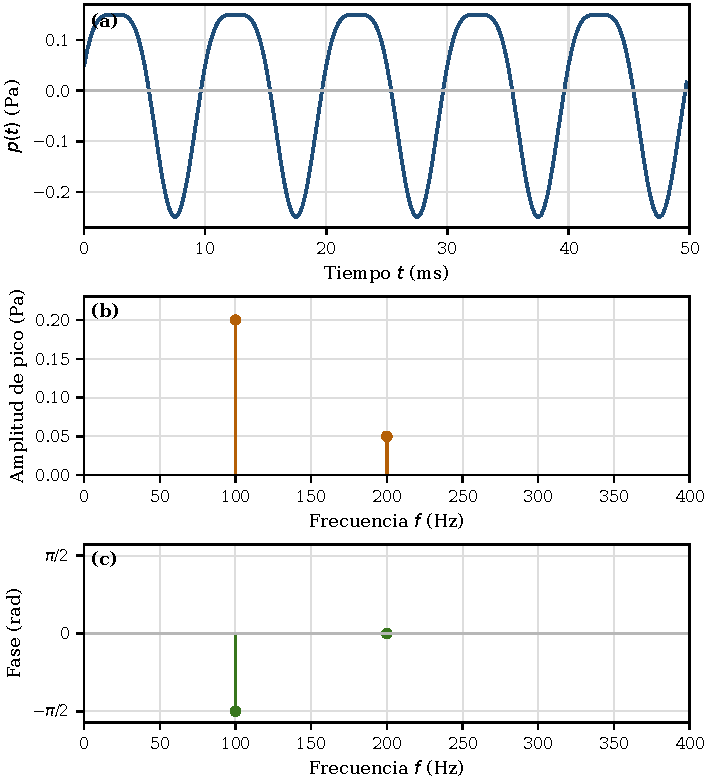
\includegraphics[width=0.96\textwidth]
        {figures/generated/unidad-5/tiempo-magnitud-fase.pdf}
    \caption{Una misma presión acústica teórica en tres representaciones:
    (a)~registro temporal; (b)~amplitud de pico de cada componente de la DFT;
    y (c)~fase de esas componentes. La señal se construyó con tonos de
    \(100\,\text{Hz}\) y \(200\,\text{Hz}\), se muestreó a
    \(f_s=4000\,\text{Hz}\) durante \(T_\mathrm{obs}=0{,}050\,\text{s}\) y se
    analizó sin ventana adicional, por lo que
    \(\Delta f=20\,\text{Hz}\). Datos sintéticos calculados; no constituyen una
    medición. Elaboración propia.}
    \label{fig:u5-tiempo-magnitud-fase}
\end{figure}

\subsection{Señales periódicas, aperiódicas y transitorias}
\label{sec:u5-periodicas-aperiodicas}

Una señal \(x(t)\), que puede representar presión, tensión eléctrica u otra
magnitud, es \textbf{periódica} si existe un intervalo positivo \(T\), medido
en segundos, tal que

\begin{equation}
    x(t+T)=x(t)
    \label{eq:u5-periodicidad}
\end{equation}

para todo instante \(t\) del modelo. El menor período positivo que satisface
esta relación se denomina período fundamental y se representará mediante
\(T_0\). Su frecuencia fundamental es

\begin{equation}
    f_0=\frac{1}{T_0},
    \label{eq:u5-fundamental-periodo}
\end{equation}

donde \(f_0\) se mide en hertz.

Una señal es \textbf{aperiódica} cuando no repite exactamente un mismo patrón
con un período fundamental. Una frase hablada completa, un golpe y una
realización de ruido son ejemplos posibles. Una señal \textbf{transitoria}
presenta cambios asociados con un comienzo, un final o una modificación
rápida. Las categorías no son excluyentes en registros reales: una vocal
sostenida puede ser aproximadamente periódica durante un intervalo y contener
transitorios al inicio y al final.

\section{Herramientas de Fourier}
\label{sec:u5-fourier}

Las herramientas de Fourier representan una señal mediante sinusoides o,
equivalentemente, mediante exponenciales complejas. Esta descomposición no
implica que un dispositivo físico separe necesariamente el sonido en piezas
independientes. Es una forma de describir y calcular propiedades de la señal.

\subsection{Serie de Fourier}
\label{sec:u5-serie-fourier}

Para una señal periódica \(x(t)\) con período fundamental \(T_0\), una forma
trigonométrica de la serie de Fourier es

\begin{equation}
    x(t)=\frac{a_0}{2}
    +\sum_{n=1}^{\infty}
    \left[
        a_n\cos(2\pi n f_0t)
        +b_n\sin(2\pi n f_0t)
    \right],
    \label{eq:u5-serie-fourier}
\end{equation}

donde \(f_0=1/T_0\), \(n\) es un entero positivo y los coeficientes
\(a_0\), \(a_n\) y \(b_n\) poseen la misma unidad que \(x(t)\). Para la
convención de la ecuación~\eqref{eq:u5-serie-fourier}, se calculan sobre un
período mediante

\begin{align}
    a_n&=\frac{2}{T_0}\int_{0}^{T_0}
        x(t)\cos(2\pi n f_0t)\,dt,
        \label{eq:u5-coef-an}\\
    b_n&=\frac{2}{T_0}\int_{0}^{T_0}
        x(t)\sin(2\pi n f_0t)\,dt.
        \label{eq:u5-coef-bn}
\end{align}

Para \(n=0\), la primera de estas expresiones determina \(a_0\) al reemplazar
el coseno por uno. El término \(a_0/2\) representa el valor medio de la señal.
Los términos con frecuencias \(nf_0\) representan componentes armónicas. Una
suma con pocos términos produce una aproximación; al agregar términos puede
reproducirse con mayor detalle la forma temporal dentro de las condiciones de
validez de la serie.

La figura~\ref{fig:u5-serie-fourier-progresiva} permite observar esa
aproximación de manera progresiva. Las oscilaciones que permanecen cerca de cada
discontinuidad no representan ruido de medición: corresponden al comportamiento
de la suma parcial y se asocian con el fenómeno de Gibbs.

\begin{figure}[htbp]
    \centering
    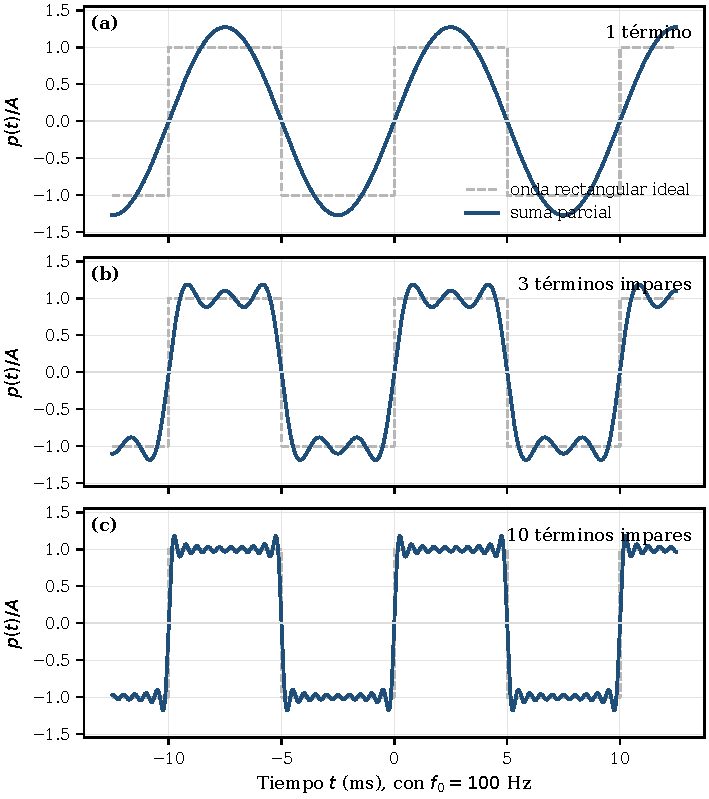
\includegraphics[width=0.96\textwidth]
        {figures/generated/unidad-5/serie-fourier-progresiva.pdf}
    \caption{Aproximación progresiva de una onda rectangular normalizada de
    frecuencia fundamental \(f_0=100\,\text{Hz}\). Se suman uno, tres y diez
    términos impares de
    \(\frac{4}{\pi}\sum_{m=0}^{M-1}
    \sin[2\pi(2m+1)f_0t]/(2m+1)\).
    Al aumentar \(M\), la suma reproduce mejor los tramos constantes, mientras
    conserva oscilaciones próximas a las discontinuidades. Modelo matemático;
    elaboración propia.}
    \label{fig:u5-serie-fourier-progresiva}
\end{figure}

\subsection{Ejemplo resuelto: periodicidad y componentes}
\label{sec:u5-ejemplo-periodicidad}

Considérese la presión

\[
    p(t)=0{,}20\,\text{Pa}\,
        \sin(2\pi\,100\,\text{Hz}\,t)
    +0{,}050\,\text{Pa}\,
        \sin(2\pi\,200\,\text{Hz}\,t+\pi/2).
\]

Las dos frecuencias son múltiplos enteros de \(100\,\text{Hz}\). El período
fundamental de la suma es

\[
    T_0=\frac{1}{100\,\text{Hz}}
       =0{,}010\,\text{s}.
\]

La componente de \(100\,\text{Hz}\) es la fundamental y la de
\(200\,\text{Hz}\) es el segundo armónico. En este ejemplo, la fundamental
también posee la mayor amplitud, pero esa coincidencia no forma parte de la
definición: otra señal podría tener un segundo armónico de mayor amplitud.

\subsection{Transformada de Fourier}
\label{sec:u5-transformada-fourier}

La transformada de Fourier permite describir señales sin exigir que repitan
exactamente un período. Para una señal \(x(t)\), se define

\begin{equation}
    X(f)=\int_{-\infty}^{\infty}
        x(t)e^{-j2\pi ft}\,dt,
    \label{eq:u5-transformada-fourier}
\end{equation}

donde \(f\) se mide en hertz y \(j\) es la unidad imaginaria,
\(j^2=-1\). Si \(x(t)\) posee una unidad física \(U\), entonces, con esta
convención, \(X(f)\) posee unidad \(U\,\text{s}\). Para una presión acústica,
por ejemplo, la transformada posee unidad \(\text{Pa}\,\text{s}\).

La transformada es una cantidad compleja y puede escribirse como

\begin{equation}
    X(f)=\lvert X(f)\rvert e^{j\phi_X(f)},
    \label{eq:u5-magnitud-fase}
\end{equation}

donde \(\lvert X(f)\rvert\) es el \textbf{espectro de magnitud} y
\(\phi_X(f)\) es el \textbf{espectro de fase}, expresado en radianes. La
magnitud informa cuánto contribuye cada frecuencia según la convención usada;
la fase informa cómo se ubican temporalmente las componentes. Dos señales
pueden compartir el mismo espectro de magnitud y diferir en fase, por lo que
no necesariamente tendrán la misma forma temporal.

Para señales periódicas ideales, la serie de Fourier resulta más directa y el
espectro se concentra en líneas discretas. Para señales aperiódicas ideales,
la transformada puede producir un espectro continuo. Un registro experimental
siempre tiene duración finita y se analiza mediante herramientas discretas.

\subsection{Muestreo, DFT y FFT}
\label{sec:u5-dft-fft}

Supóngase que una señal se muestrea \(f_s\) veces por segundo. La frecuencia
de muestreo \(f_s\) se mide en hertz. Si se conservan \(N\) muestras, la
duración observada es

\begin{equation}
    T_\mathrm{obs}=\frac{N}{f_s},
    \label{eq:u5-duracion-registro}
\end{equation}

donde \(T_\mathrm{obs}\) se mide en segundos. La transformada discreta de
Fourier (DFT) produce valores en frecuencias discretas o \textbf{bins}. La
transformada rápida de Fourier (FFT) es un algoritmo eficiente para calcular
esa DFT; no es una transformada física diferente.

La separación entre bins es

\begin{equation}
    \Delta f=\frac{f_s}{N}
            =\frac{1}{T_\mathrm{obs}},
    \label{eq:u5-resolucion-frecuencial}
\end{equation}

donde \(\Delta f\) se mide en hertz. Una observación más larga reduce
\(\Delta f\) y permite separar componentes cercanas con mayor facilidad. Esta
\textbf{resolución frecuencial} no es lo mismo que la precisión o
incertidumbre con la que se estima una frecuencia. La precisión también
depende, entre otros factores, del ruido, la estabilidad de la señal, el
muestreo, la ventana y el método de estimación.

\subsection{Ventanas, fuga espectral y espectrograma}
\label{sec:u5-ventanas-espectrograma}

Al recortar una señal se multiplica implícitamente por una ventana temporal.
Si el registro no contiene un número entero de períodos, la energía asociada
con una componente puede distribuirse entre varios bins. Este efecto se
denomina \textbf{fuga espectral}.

Ventanas como Hann reducen ciertos lóbulos de la fuga, pero ensanchan la
respuesta alrededor de cada componente. Por lo tanto, usar una ventana
implica un compromiso; no ``corrige'' todos los problemas de la medición.

Un \textbf{espectrograma} se obtiene dividiendo una señal en segmentos,
aplicando una ventana y calculando un espectro para cada segmento. Su eje
horizontal representa tiempo, su eje vertical frecuencia y el color
representa una magnitud espectral declarada. Segmentos largos mejoran la
resolución frecuencial, mientras que segmentos cortos permiten seguir cambios
temporales más rápidos.

Este compromiso se observa en la
figura~\ref{fig:u5-compromiso-tiempo-frecuencia}. Se analiza la misma señal
sintética con dos ventanas Hann: la ventana corta ubica mejor el instante del
cambio, pero no separa con claridad las dos componentes próximas; la larga
separa las líneas, aunque extiende temporalmente la transición.

\begin{figure}[htbp]
    \centering
    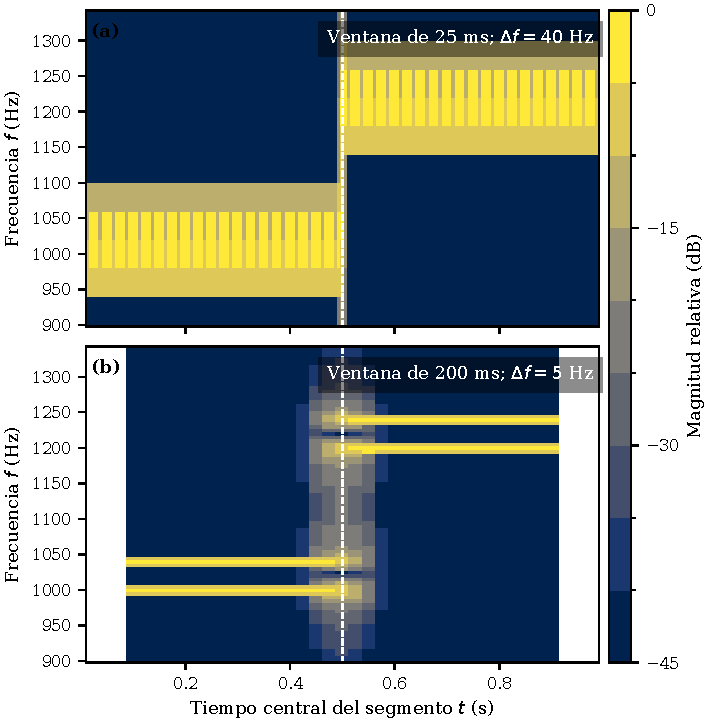
\includegraphics[width=0.96\textwidth]
        {figures/generated/unidad-5/compromiso-tiempo-frecuencia.pdf}
    \caption{Compromiso entre resolución temporal y frecuencial en dos
    espectrogramas de la misma señal teórica, muestreada a
    \(f_s=8000\,\text{Hz}\). Antes de \(0{,}5\,\text{s}\) contiene componentes
    de \(1000\,\text{Hz}\) y \(1040\,\text{Hz}\); después contiene
    \(1200\,\text{Hz}\) y \(1240\,\text{Hz}\). La ventana Hann de
    \(25\,\text{ms}\) produce \(\Delta f=40\,\text{Hz}\); la de
    \(200\,\text{ms}\), \(\Delta f=5\,\text{Hz}\). El color expresa magnitud
    relativa al máximo de cada análisis. Datos sintéticos; elaboración propia.}
    \label{fig:u5-compromiso-tiempo-frecuencia}
\end{figure}

\subsection{Ejemplo resuelto: resolución frecuencial}
\label{sec:u5-ejemplo-resolucion}

Se registra una señal con \(f_s=8000\,\text{Hz}\) y \(N=2000\) muestras.
La duración y la separación entre bins son

\[
    T_\mathrm{obs}=\frac{2000}{8000\,\text{Hz}}
                  =0{,}250\,\text{s},
\]

\[
    \Delta f=\frac{8000\,\text{Hz}}{2000}
            =4{,}0\,\text{Hz}.
\]

Si se mantiene \(f_s=8000\,\text{Hz}\) y se aumenta el registro a
\(N=8000\) muestras, entonces \(T_\mathrm{obs}=1{,}00\,\text{s}\) y
\(\Delta f=1{,}0\,\text{Hz}\). La resolución nominal mejora, aunque ello no
garantiza por sí solo que una estimación sea exacta.

\subsection{Nivel por bin y nivel por banda}
\label{sec:u5-bin-banda}

Un bin representa un intervalo asociado con la resolución del análisis. Si se
modifica \(T_\mathrm{obs}\), cambia \(\Delta f\) y puede cambiar la cantidad
espectral informada en cada bin. Por eso, un ``nivel por bin'' no debe
compararse entre configuraciones sin declarar duración, ventana y
normalización.

Una banda reúne un intervalo de frecuencias definido por un límite inferior
\(f_L\) y uno superior \(f_H\), ambos en hertz. Cuando los valores de los bins
representan contribuciones cuadráticas no correlacionadas \(q_k\), la
contribución de la banda es

\begin{equation}
    q_B=\sum_{k\in B}q_k.
    \label{eq:u5-suma-bins}
\end{equation}

Si cada contribución ya está expresada como un nivel
\(L_k=10\log_{10}(q_k/q_\mathrm{ref})\), el nivel total de la banda se obtiene
mediante

\begin{equation}
    L_B=10\log_{10}
    \left(\sum_{k\in B}10^{L_k/10}\right).
    \label{eq:u5-nivel-banda}
\end{equation}

No corresponde promediar aritméticamente los decibeles. Tampoco deben sumarse
amplitudes sin considerar fase cuando las componentes son coherentes, tal como
se estudió en la Unidad~\ref{chap:unidad-4}.

\section{Espectro de una señal y respuesta de un sistema}
\label{sec:u5-espectro-respuesta}

El \textbf{espectro de una señal} describe la distribución frecuencial de un
registro particular. Si se graba una vocal, el espectro depende de la fuente,
del tracto vocal, de la radiación, del micrófono, del ambiente y del segmento
analizado.

La \textbf{respuesta en frecuencia de un sistema} describe, en cambio, cómo
ese sistema modifica señales de distintas frecuencias. Para un sistema lineal
e invariante en el tiempo, con entrada \(x(t)\), salida \(y(t)\) y
transformadas \(X(f)\) e \(Y(f)\), se define

\begin{equation}
    H(f)=\frac{Y(f)}{X(f)}
    \qquad\text{cuando }X(f)\neq0.
    \label{eq:u5-respuesta-frecuencia}
\end{equation}

La magnitud \(\lvert H(f)\rvert\) informa el cambio de amplitud y la fase
\(\phi_H(f)\), en radianes, informa el cambio de fase. Si entrada y salida
representan la misma magnitud física, el cociente es adimensional y su
ganancia de amplitud puede expresarse como

\begin{equation}
    G(f)=20\log_{10}\lvert H(f)\rvert,
    \label{eq:u5-ganancia-respuesta}
\end{equation}

donde \(G(f)\) se expresa en decibeles. Una respuesta no puede deducirse de la
salida solamente: se necesita conocer la entrada o emplear un procedimiento
de medición equivalente.

La figura~\ref{fig:u5-espectro-respuesta-sistema} compara las tres cantidades
con una escala común. Los paneles de entrada y salida son espectros de señales;
el panel central es una propiedad del sistema dentro del modelo lineal.

\begin{figure}[htbp]
    \centering
    % Propósito: distinguir los espectros de entrada y salida de la respuesta en
% frecuencia del sistema que los relaciona.
% Origen: Y(f)=X(f)H(f). Se usan magnitudes normalizadas y datos teóricos:
% |X|=(0,8;0,8;0,8), |H|=(1;0,5;0,25) para f=(0,5;1;2) kHz;
% por lo tanto |Y|=(0,8;0,4;0,2).
% Esquema matemático; no representa un dispositivo ni una medición real.
% Descripción accesible: tres paneles muestran, de izquierda a derecha, un
% espectro de entrada con tres componentes iguales, una respuesta de sistema
% que atenúa progresivamente esas frecuencias y un espectro de salida cuyos
% componentes son los productos de entrada y respuesta. La figura enfatiza que
% el espectro pertenece a una señal y H pertenece al sistema.
\begin{tikzpicture}[font=\small,>=stealth,x=1cm,y=1cm]
    \node[font=\bfseries] at (5.75,4.75)
        {\(\lvert Y(f)\rvert=\lvert X(f)\rvert\,\lvert H(f)\rvert\)};

    \begin{scope}[shift={(0.15,0)}]
        \node[font=\bfseries] at (1.65,4.05) {Entrada: \(\lvert X(f)\rvert\)};
        \draw[->] (0.35,0.75) -- (3.05,0.75);
        \draw[->] (0.55,0.55) -- (0.55,3.45);
        \node[rotate=90] at (0.10,2.10) {magnitud};
        \draw[very thick] (1.05,0.75) -- (1.05,2.90);
        \draw[very thick] (1.75,0.75) -- (1.75,2.90);
        \draw[very thick] (2.55,0.75) -- (2.55,2.90);
        \foreach \x/\lab in {1.05/0{,}5,1.75/1,2.55/2}
            \node[below] at (\x,0.72) {\lab};
        \node[anchor=west] at (0.62,2.90) {\(0{,}8\)};
        \node at (1.75,0.12) {\(f\) (kHz)};
    \end{scope}

    \node[font=\Large] at (3.75,2.10) {\(\times\)};

    \begin{scope}[shift={(4.05,0)}]
        \node[font=\bfseries] at (1.65,4.05) {Sistema: \(\lvert H(f)\rvert\)};
        \draw[->] (0.35,0.75) -- (3.05,0.75);
        \draw[->] (0.55,0.55) -- (0.55,3.45);
        \node[rotate=90] at (0.10,2.10) {ganancia};
        \draw[very thick] (1.05,0.75) -- (1.05,3.15);
        \draw[very thick] (1.75,0.75) -- (1.75,1.95);
        \draw[very thick] (2.55,0.75) -- (2.55,1.35);
        \draw[thick] (1.05,3.15) -- (1.75,1.95) -- (2.55,1.35);
        \foreach \x/\lab in {1.05/0{,}5,1.75/1,2.55/2}
            \node[below] at (\x,0.72) {\lab};
        \node[anchor=east] at (0.50,3.15) {\(1\)};
        \node at (1.75,0.12) {\(f\) (kHz)};
    \end{scope}

    \node[font=\Large] at (7.65,2.10) {\(=\)};

    \begin{scope}[shift={(7.95,0)}]
        \node[font=\bfseries] at (1.65,4.05) {Salida: \(\lvert Y(f)\rvert\)};
        \draw[->] (0.35,0.75) -- (3.05,0.75);
        \draw[->] (0.55,0.55) -- (0.55,3.45);
        \node[rotate=90] at (0.10,2.10) {magnitud};
        \draw[very thick] (1.05,0.75) -- (1.05,2.90);
        \draw[very thick] (1.75,0.75) -- (1.75,1.83);
        \draw[very thick] (2.55,0.75) -- (2.55,1.29);
        \foreach \x/\lab in {1.05/0{,}5,1.75/1,2.55/2}
            \node[below] at (\x,0.72) {\lab};
        \node[anchor=west] at (0.62,2.90) {\(0{,}8\)};
        \node at (1.75,0.12) {\(f\) (kHz)};
    \end{scope}

    \node[align=center] at (5.75,-0.35)
        {espectros de señales \(\lvert X\rvert,\lvert Y\rvert\)
         \(\quad\neq\quad\) respuesta del sistema \(\lvert H\rvert\)};
\end{tikzpicture}

    \caption{Relación entre los espectros de magnitud de entrada y salida y la
    magnitud de la respuesta de un sistema. En este ejemplo teórico,
    \(\lvert Y(f)\rvert=\lvert X(f)\rvert\lvert H(f)\rvert\) en tres
    frecuencias. Conocer solo \(\lvert Y(f)\rvert\) no permite separar cuánto
    corresponde a la señal de entrada y cuánto al sistema. Magnitudes
    normalizadas; elaboración propia.}
    \label{fig:u5-espectro-respuesta-sistema}
\end{figure}

Si un sistema introduce únicamente un retraso \(\tau\), medido en segundos,
la magnitud de su respuesta ideal permanece igual a uno y el cambio de fase es

\begin{equation}
    \phi_H(f)=-2\pi f\tau,
    \label{eq:u5-fase-retardo}
\end{equation}

donde \(\phi_H(f)\) se expresa en radianes. Este ejemplo muestra que una
respuesta puede modificar la fase sin modificar la magnitud.

En producción vocal, una descripción introductoria considera una fuente
glótica y un tracto vocal que actúa como sistema acústico. Los formantes se
relacionan con resonancias del tracto y suelen observarse en la envolvente
espectral, mientras que las líneas armónicas se relacionan con la periodicidad
de la fuente. La interpretación de formantes y otros parámetros de voz
requiere definir la vocal, el hablante, el método de análisis y el alcance
clínico, además de incorporar bibliografía especializada~\cite{brockmann2011}.

\subsection{Ejemplo resuelto: ganancia a una frecuencia}
\label{sec:u5-ejemplo-respuesta}

Un sistema recibe un tono de \(1000\,\text{Hz}\) con presión eficaz de entrada
\(p_\mathrm{in}=0{,}020\,\text{Pa}\) y produce una presión eficaz de salida
\(p_\mathrm{out}=0{,}010\,\text{Pa}\), medidas bajo las mismas condiciones.
La magnitud de la respuesta a esa frecuencia es

\[
    \lvert H(1000\,\text{Hz})\rvert
    =\frac{0{,}010\,\text{Pa}}{0{,}020\,\text{Pa}}
    =0{,}50.
\]

La ganancia es

\[
    G(1000\,\text{Hz})
    =20\log_{10}(0{,}50)
    \approx-6{,}02\,\text{dB}.
\]

El resultado indica una reducción de amplitud a \(1000\,\text{Hz}\). No
describe el espectro completo de la entrada ni permite conocer la respuesta
del sistema en otras frecuencias.

\section{Componentes espectrales}
\label{sec:u5-componentes}

\begin{description}[style=nextline]
    \item[\textbf{Frecuencia fundamental (\(f_0\)):}]
    inversa del período fundamental \(T_0\) de una señal periódica. No tiene
    que coincidir con la componente de mayor amplitud.

    \item[\textbf{Armónico:}]
    componente cuya frecuencia es \(nf_0\), donde \(n\) es un entero
    positivo. El primer armónico corresponde a \(f_0\), si esa componente está
    presente.

    \item[\textbf{Parcial:}]
    componente sinusoidal identificable en una señal compleja. Los parciales
    pueden ser armónicos o inarmónicos.

    \item[\textbf{Sobretono:}]
    parcial situado por encima de la fundamental en el uso musical y
    acústico habitual. El primer sobretono es el segundo parcial, por lo que
    no debe confundirse con el primer armónico.

    \item[\textbf{Parcial inarmónico:}]
    componente cuya frecuencia no coincide con un múltiplo entero de
    \(f_0\).
\end{description}

Una señal periódica puede conservar su periodicidad aunque la línea en
\(f_0\) tenga amplitud nula. En ese caso se habla de una fundamental ausente:
las separaciones entre armónicos todavía pueden revelar la periodicidad. El
\emph{pitch} asociado con este tipo de estímulos es un fenómeno perceptual y
se desarrollará en el capítulo dedicado a psicoacústica; no se identifica con
una línea espectral por definición.

La figura~\ref{fig:u5-componentes-espectrales} reúne tres casos con igual
escala. Permite comprobar que el componente de mayor amplitud no define
\(f_0\), que no todo parcial es armónico y que una periodicidad puede
manifestarse por la separación entre líneas aun si falta la componente
fundamental.

\begin{figure}[htbp]
    \centering
    % Propósito: diferenciar armónicos, parciales, sobretonos, componente de mayor
% amplitud y fundamental ausente mediante espectros con una misma escala.
% Origen: datos teóricos de magnitud normalizada. Panel armónico:
% f=(100,200,300,400) Hz y A=(0,45;1;0,60;0,30). Panel inarmónico:
% f=(100,235,370,520) Hz y A=(0,60;1;0,55;0,30). Fundamental ausente:
% f=(200,300,400) Hz y A=(1;0,60;0,40), con separación de 100 Hz.
% No representa sonidos medidos ni instrumentos particulares.
% Descripción accesible: el primer panel tiene líneas en múltiplos de 100 Hz y
% muestra que el segundo armónico puede superar a la fundamental. El segundo
% presenta parciales que no son múltiplos enteros. El tercero omite la línea de
% 100 Hz, pero conserva líneas separadas 100 Hz, de modo que la periodicidad
% fundamental puede inferirse aunque esa componente esté ausente.
\begin{tikzpicture}[font=\small,>=stealth,x=0.018cm,y=1.45cm]
    \begin{scope}[shift={(0,4.55)}]
        \node[anchor=west,font=\bfseries] at (0,1.32)
            {(a) Serie armónica, \(f_0=100\,\text{Hz}\)};
        \draw[->] (0,0) -- (570,0) node[below right] {\(f\) (Hz)};
        \draw[->] (0,-0.05) -- (0,1.18);
        \node[rotate=90] at (-18,0.58) {\(A/A_{\max}\)};
        \foreach \f/\a in {100/0.45,200/1.00,300/0.60,400/0.30}
            \draw[very thick] (\f,0) -- (\f,\a);
        \foreach \f in {100,200,300,400,500}
            \node[below] at (\f,-0.01) {\f};
        \node[above,align=center] at (100,0.45) {\(f_0\)};
        \node[anchor=west,align=left] at (208,0.90)
            {\(2f_0\), 1.er sobretono};
    \end{scope}

    \begin{scope}[shift={(0,2.20)}]
        \node[anchor=west,font=\bfseries] at (0,1.32)
            {(b) Parciales inarmónicos};
        \draw[->] (0,0) -- (570,0) node[below right] {\(f\) (Hz)};
        \draw[->] (0,-0.05) -- (0,1.18);
        \node[rotate=90] at (-18,0.58) {\(A/A_{\max}\)};
        \foreach \f/\a in {100/0.60,235/1.00,370/0.55,520/0.30}
            \draw[very thick] (\f,0) -- (\f,\a);
        \foreach \f in {100,235,370,520}
            \node[below] at (\f,-0.01) {\f};
        \node[anchor=west] at (245,0.90) {parcial de mayor amplitud};
    \end{scope}

    \begin{scope}[shift={(0,-0.15)}]
        \node[anchor=west,font=\bfseries] at (0,1.32)
            {(c) Fundamental ausente};
        \draw[->] (0,0) -- (570,0) node[below right] {\(f\) (Hz)};
        \draw[->] (0,-0.05) -- (0,1.18);
        \node[rotate=90] at (-18,0.58) {\(A/A_{\max}\)};
        \draw[very thick,densely dashed] (100,0) -- (100,0.72);
        \foreach \f/\a in {200/1.00,300/0.60,400/0.40}
            \draw[very thick] (\f,0) -- (\f,\a);
        \foreach \f in {100,200,300,400,500}
            \node[below] at (\f,-0.01) {\f};
        \node[above,align=center] at (100,0.72)
            {\(f_0\) inferida\\sin línea};
        \draw[<->] (200,0.18) -- (300,0.18)
            node[midway,above] {\(100\,\text{Hz}\)};
    \end{scope}
\end{tikzpicture}

    \caption{Comparación de espectros de líneas teóricos con magnitud
    normalizada. (a)~Serie armónica de \(f_0=100\,\text{Hz}\), cuyo segundo
    armónico posee la mayor amplitud; el primer sobretono coincide aquí con el
    segundo armónico. (b)~Parciales inarmónicos, que no siguen múltiplos
    enteros. (c)~Fundamental ausente: no aparece una línea en
    \(100\,\text{Hz}\), pero las componentes conservan esa separación.
    Elaboración propia; no son registros de fuentes reales.}
    \label{fig:u5-componentes-espectrales}
\end{figure}

\section{Rangos de frecuencia y rangos dinámicos}
\label{sec:u5-rangos}

\subsection{Infrasonido, rango audible y ultrasonido}
\label{sec:u5-infra-audible-ultra}

Se usa de manera convencional \(20\,\text{Hz}\) como frontera entre
infrasonido y rango audible, y \(20\,\text{kHz}\) como frontera entre rango
audible y ultrasonido; estos límites son aproximados y requieren una fuente
académica que declare las condiciones de escucha~\cite{oxenham2018,iso226_2023}.

El término \textbf{infrasonido} describe frecuencias inferiores a la frontera
convencional de \(20\,\text{Hz}\). No significa que toda señal de esa región
sea necesariamente imperceptible: la detección puede depender del
nivel, la duración, la distorsión del sistema y la presencia de vibración~\cite{oxenham2018,iso226_2023}.

El \textbf{rango audible} no es idéntico para todas las personas ni para todos
los niveles. La sensibilidad varía con la frecuencia y con características
del oyente. Estas dependencias perceptuales se estudiarán posteriormente.

El \textbf{ultrasonido} corresponde a frecuencias superiores a la frontera
convencional de \(20\,\text{kHz}\). Una aplicación médica general es la
formación de imágenes mediante ultrasonido; las otoemisiones acústicas no
deben presentarse como ejemplo de ultrasonido sin especificar las frecuencias
de estímulo y registro.

\subsection{Qué significa rango dinámico}
\label{sec:u5-rango-dinamico}

El \textbf{rango dinámico} compara un nivel superior y uno inferior que deben
estar definidos mediante la misma magnitud, referencia y condición de
medición. Si \(L_\mathrm{sup}\) y \(L_\mathrm{inf}\) son esos niveles, el
rango dinámico es

\begin{equation}
    R_D=L_\mathrm{sup}-L_\mathrm{inf},
    \label{eq:u5-rango-dinamico}
\end{equation}

y se expresa en decibeles. La resta informa una relación; no debe interpretarse
sin conocer cómo se eligieron los extremos.

\begin{description}[style=nextline]
    \item[\textbf{Rango dinámico vocal:}]
    diferencia entre niveles relevantes de una producción vocal bajo una
    condición declarada. Deben especificarse distancia, dirección,
    ponderación, descriptor temporal y tarea de emisión.

    \item[\textbf{Rango dinámico instrumental:}]
    diferencia entre niveles relevantes producidos por un instrumento bajo
    condiciones definidas. No es un valor universal del instrumento: depende
    de técnica, nota, sala y posición de medición.

    \item[\textbf{Rango dinámico auditivo:}]
    intervalo entre un límite inferior de audibilidad y un límite superior
    definido, por ejemplo un nivel de incomodidad, para una frecuencia,
    estímulo y oyente determinados. No corresponde reemplazar automáticamente
    el límite superior por un ``umbral de dolor'' universal.
\end{description}

Los valores numéricos de rangos vocales, instrumentales y auditivos
deben incorporarse solo después de seleccionar fuentes, condiciones de
medición y población de referencia~\cite{oxenham2018,iso226_2023}.

\section{Bandas de octava y tercio de octava}
\label{sec:u5-bandas}

Agrupar frecuencias en bandas permite resumir un espectro con una resolución
relativa aproximadamente constante. Una banda se define mediante su límite
inferior \(f_L\), su límite superior \(f_H\) y su frecuencia central
geométrica \(f_c\), todas medidas en hertz:

\begin{equation}
    f_c=\sqrt{f_Lf_H}.
    \label{eq:u5-centro-geometrico}
\end{equation}

Para una fracción \(1/b\) de octava, la razón entre límites es

\begin{equation}
    \frac{f_H}{f_L}=2^{1/b}.
    \label{eq:u5-razon-banda}
\end{equation}

Los límites alrededor de \(f_c\) son

\begin{equation}
    f_L=f_c\,2^{-1/(2b)},
    \qquad
    f_H=f_c\,2^{1/(2b)}.
    \label{eq:u5-limites-banda}
\end{equation}

El ancho de banda \(B\), medido en hertz, se define como

\begin{equation}
    B=f_H-f_L.
    \label{eq:u5-ancho-banda}
\end{equation}

Para una octava, \(b=1\) y \(f_H/f_L=2\). Para un tercio de octava,
\(b=3\) y \(f_H/f_L=2^{1/3}\). Los instrumentos normalizados usan
series de frecuencias centrales nominales y requisitos de tolerancia que deben
documentarse con la edición aplicable de la norma de filtros de banda~\cite{iec61260_1_2014}.

\subsection{Ejemplo resuelto: tercio de octava}
\label{sec:u5-ejemplo-tercio}

Para \(f_c=1000\,\text{Hz}\) y \(b=3\):

\[
    f_L=1000\,\text{Hz}\,2^{-1/6}
       \approx890{,}9\,\text{Hz},
\]

\[
    f_H=1000\,\text{Hz}\,2^{1/6}
       \approx1122{,}5\,\text{Hz}.
\]

Por lo tanto,

\[
    B\approx1122{,}5\,\text{Hz}-890{,}9\,\text{Hz}
      \approx231{,}6\,\text{Hz}.
\]

Los valores redondeados \(891\,\text{Hz}\) y \(1122\,\text{Hz}\) son límites
aproximados; el ancho no es \(176\,\text{Hz}\).

La división completa se muestra en la
figura~\ref{fig:u5-bandas-octava-tercio}. Sobre el eje logarítmico, los tres
tercios ocupan igual longitud porque comparten la misma razón entre límites;
sus anchos absolutos en hertz, en cambio, no son iguales.

\begin{figure}[htbp]
    \centering
    % Propósito: mostrar que una octava puede dividirse en tres tercios contiguos
% sobre un eje logarítmico y que el ancho absoluto crece con la frecuencia.
% Origen: ecuaciones f_L=f_c 2^{-1/(2b)}, f_H=f_c 2^{1/(2b)} y B=f_H-f_L.
% Para la octava centrada en 1000 Hz: límites 707,1 y 1414,2 Hz.
% Los tres tercios tienen centros 793,7; 1000 y 1259,9 Hz, límites comunes
% 707,1; 890,9; 1122,5; 1414,2 Hz y anchos 183,8; 231,6; 291,8 Hz.
% Esquema matemático sobre eje logarítmico; no representa filtros medidos.
% Descripción accesible: una barra superior abarca la octava de 707,1 a
% 1414,2 Hz alrededor de 1000 Hz. Debajo, tres barras contiguas ocupan el mismo
% intervalo sobre el eje logarítmico. Aunque tienen la misma razón entre
% límites, sus anchos en hertz aumentan hacia frecuencias más altas.
\begin{tikzpicture}[font=\small,>=stealth,x=1cm,y=1cm]
    \node[anchor=west,font=\bfseries] at (1.40,4.55)
        {Octava (\(b=1\))};

    \draw[fill=black!10] (1.40,3.35) rectangle (9.80,4.05);
    \draw[very thick] (1.40,3.35) rectangle (9.80,4.05);
    \draw[densely dashed] (5.60,3.25) -- (5.60,4.18);
    \node at (5.60,3.70) {\(B=707{,}1\,\text{Hz}\)};
    \node[above] at (1.40,4.05) {\(f_L\)};
    \node[above] at (5.60,4.05) {\(f_c\)};
    \node[above] at (9.80,4.05) {\(f_H\)};

    \node[font=\bfseries] at (5.60,2.85)
        {Tres tercios de octava contiguos};
    \draw[fill=black!6] (1.40,1.55) rectangle (4.20,2.35);
    \draw[fill=black!14] (4.20,1.55) rectangle (7.00,2.35);
    \draw[fill=black!22] (7.00,1.55) rectangle (9.80,2.35);
    \draw[very thick] (1.40,1.55) rectangle (9.80,2.35);
    \draw[very thick] (4.20,1.55) -- (4.20,2.35);
    \draw[very thick] (7.00,1.55) -- (7.00,2.35);
    \node[align=center] at (2.80,1.95)
        {\(f_c=793{,}7\,\text{Hz}\)\\\(B=183{,}8\,\text{Hz}\)};
    \node[align=center] at (5.60,1.95)
        {\(f_c=1000\,\text{Hz}\)\\\(B=231{,}6\,\text{Hz}\)};
    \node[align=center] at (8.40,1.95)
        {\(f_c=1259{,}9\,\text{Hz}\)\\\(B=291{,}8\,\text{Hz}\)};

    \draw[->] (0.80,0.70) -- (10.20,0.70);
    \foreach \x/\lab in {
        1.40/707{,}1,
        4.20/890{,}9,
        7.00/1122{,}5,
        9.80/1414{,}2
    }{
        \draw (\x,0.62) -- (\x,0.78);
        \node[below] at (\x,0.62) {\lab};
        \draw[densely dotted] (\x,0.80) -- (\x,1.50);
    }
    \node[align=center] at (5.60,-0.05)
        {\(f\) (Hz), escala logarítmica;
         cada tercio cumple \(f_H/f_L=2^{1/3}\)};
\end{tikzpicture}

    \caption{Una octava centrada en \(1000\,\text{Hz}\) y su división en tres
    tercios contiguos. Los límites se calcularon con
    \(f_L=f_c2^{-1/(2b)}\) y \(f_H=f_c2^{1/(2b)}\). Las bandas tienen el mismo
    ancho relativo sobre el eje logarítmico, pero \(B=f_H-f_L\) aumenta con la
    frecuencia. Valores teóricos redondeados a \(0{,}1\,\text{Hz}\);
    elaboración propia.}
    \label{fig:u5-bandas-octava-tercio}
\end{figure}

\section{Filtros y respuesta en frecuencia}
\label{sec:u5-filtros}

Un filtro es un sistema que modifica componentes de una señal según la
frecuencia. Un filtro \textbf{ideal} cambia abruptamente entre paso y rechazo.
Un filtro \textbf{real} posee regiones de transición, atenuación finita y una
respuesta de fase que puede modificar la forma temporal.

\begin{description}[style=nextline]
    \item[\textbf{Pasa bajos:}]
    conserva una banda de bajas frecuencias y atenúa frecuencias por encima de
    su transición.

    \item[\textbf{Pasa altos:}]
    conserva una banda de altas frecuencias y atenúa frecuencias por debajo de
    su transición.

    \item[\textbf{Pasa banda:}]
    conserva un intervalo entre un límite inferior \(f_L\) y uno superior
    \(f_H\).

    \item[\textbf{Elimina banda o rechazo de banda:}]
    atenúa un intervalo entre \(f_L\) y \(f_H\) y conserva frecuencias por
    debajo y por encima. Un filtro \emph{notch} es un rechazo relativamente
    estrecho.
\end{description}

La \textbf{frecuencia de corte} debe asociarse con un criterio de atenuación
declarado. En modelos comunes se usa el punto de \(-3\,\text{dB}\), pero esa
convención no es universal para todo filtro o instrumento. En filtros pasa
banda y elimina banda se requieren, como mínimo, dos frecuencias límite. Su
frecuencia central puede definirse geométricamente como

\[
    f_c=\sqrt{f_Lf_H},
\]

y su ancho como \(B=f_H-f_L\), ambos con las mismas definiciones y unidades
empleadas para las bandas.

La figura~\ref{fig:u5-filtros-ideales-reales} compara el salto matemático ideal
con modelos no ideales que poseen transición. Las líneas verticales sirven para
ubicar \(f_c\), \(f_L\) y \(f_H\); no deben interpretarse como especificaciones
de un instrumento particular.

\begin{figure}[htbp]
    \centering
    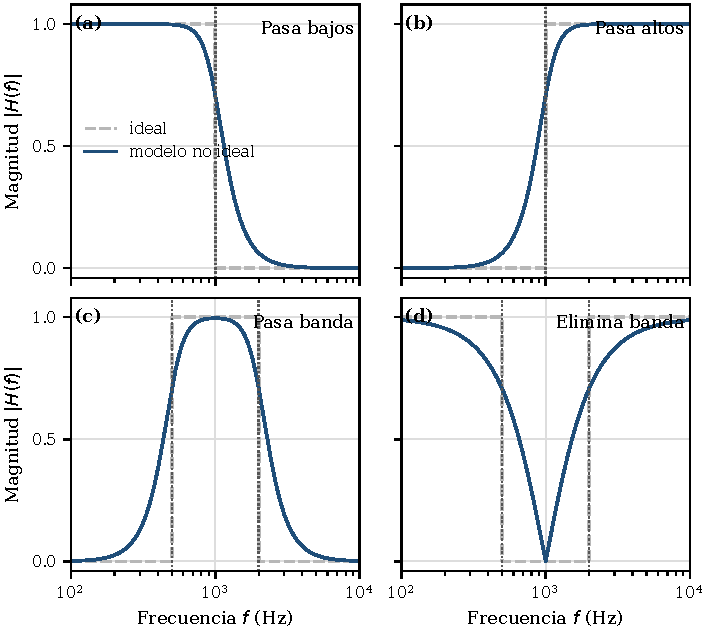
\includegraphics[width=0.96\textwidth]
        {figures/generated/unidad-5/filtros-ideales-reales.pdf}
    \caption{Respuestas de magnitud ideales y modelos analíticos no ideales para
    filtros pasa bajos, pasa altos, pasa banda y elimina banda. Los pasa bajos y
    pasa altos usan modelos Butterworth de cuarto orden con
    \(f_c=1000\,\text{Hz}\); el pasa banda combina límites de
    \(f_L=500\,\text{Hz}\) y \(f_H=2000\,\text{Hz}\), y el rechazo usa un
    modelo de segundo orden con \(f_c=\sqrt{f_Lf_H}=1000\,\text{Hz}\).
    Curvas teóricas, no respuestas medidas; elaboración propia.}
    \label{fig:u5-filtros-ideales-reales}
\end{figure}

\subsection{Filtrado, ponderación y filtrado audiométrico}
\label{sec:u5-filtros-ponderacion-audiometria}

Estas operaciones pueden usar filtros, pero no tienen el mismo propósito:

\begin{description}[style=nextline]
    \item[\textbf{Filtrado de una señal:}]
    modifica el contenido espectral de la señal que se procesa o reproduce.

    \item[\textbf{Ponderación frecuencial de una medición:}]
    aplica una respuesta estandarizada antes de calcular e informar un nivel.
    La ponderación debe aparecer en el símbolo o en la unidad informada.

    \item[\textbf{Filtrado audiométrico:}]
    forma parte de la generación o control de estímulos de un audiómetro, por
    ejemplo al delimitar una banda de ruido. Sus requisitos dependen del
    equipo, del estímulo y de la calibración audiométrica.
\end{description}

Una ponderación A no convierte un nivel en dB SPL a dB HL. El nivel de audición
en dB HL depende de frecuencia, transductor y referencias de calibración
específicas.

\section{Ponderaciones frecuenciales A, C y Z}
\label{sec:u5-ponderaciones}

Una ponderación frecuencial es una respuesta de medición definida en función
de la frecuencia. Si \(L_Z(f)\) es el nivel de un tono medido con ponderación
Z y \(A(f)\) es la corrección de la ponderación A a esa frecuencia, expresada
en decibeles, entonces, bajo las mismas condiciones,

\begin{equation}
    L_A(f)=L_Z(f)+A(f).
    \label{eq:u5-correccion-ponderacion}
\end{equation}

La ponderación A atenúa con fuerza las bajas frecuencias y modifica también la
respuesta en otras regiones. La ponderación C posee una respuesta más plana
en una región amplia, pero tampoco es una medición sin filtro. La ponderación
Z es una respuesta nominalmente plana dentro de un intervalo y unas
tolerancias especificadas; no representa ``el sonido real'' sin límites.

Las respuestas nominales, los límites de aceptación, el intervalo de
frecuencias y las denominaciones de A, C y Z se especifican en la edición
aplicable de la norma de sonómetros~\cite{iec61672_1_2013}.

Para una señal de banda ancha no corresponde tomar un nivel total y agregar
una única corrección elegida de una tabla. La ponderación actúa de manera
diferente en cada frecuencia; el instrumento filtra la señal y luego realiza
la integración energética.

\subsection{Ejemplo resuelto: corrección para un tono}
\label{sec:u5-ejemplo-ponderacion}

La tabla 3 de IEC 61672-1:2013 establece, como valor nominal de la
ponderación A a \(63\,\text{Hz}\),
\(A(63\,\text{Hz})=-26{,}2\,\text{dB}\)~\cite{iec61672_1_2013}. Si un tono de
\(63\,\text{Hz}\) produce \(L_Z=80{,}0\,\text{dB(Z)}\), entonces

\[
    L_A=80{,}0\,\text{dB(Z)}-26{,}2\,\text{dB}
       =53{,}8\,\text{dB(A)}.
\]

El cálculo se aplica a ese tono y a la corrección proporcionada. No implica
que cualquier sonido de \(80\,\text{dB(Z)}\) produzca
\(53{,}8\,\text{dB(A)}\).

% TODO(figure): evaluar una figura original de las curvas nominales A, C y Z
% calculadas con las expresiones del anexo E de IEC 61672-1:2013; diferenciar
% esas curvas de los límites de aceptación de un instrumento.

\section{Sonómetro}
\label{sec:u5-sonometro}

Un sonómetro recibe una señal de micrófono y la procesa para informar niveles
acústicos definidos. Una cadena funcional básica incluye:

\begin{enumerate}
    \item \textbf{micrófono:} convierte la presión acústica local, en
    pascales, en una señal eléctrica. Un micrófono con corrección de campo
    libre no elimina las reflexiones del ambiente;
    \item \textbf{preamplificación y conversión:} adapta y, en instrumentos
    digitales, muestrea la señal;
    \item \textbf{ponderación frecuencial:} aplica A, C, Z u otra respuesta
    disponible y declarada;
    \item \textbf{detector o integrador:} calcula una medida cuadrática,
    temporal o de exposición;
    \item \textbf{ponderación temporal:} determina cómo responde la indicación
    ante cambios rápidos;
    \item \textbf{visualización y almacenamiento:} informa la magnitud, la
    ponderación, el intervalo temporal y, cuando corresponda, incertidumbre o
    estado del instrumento.
\end{enumerate}

La figura~\ref{fig:u5-cadena-sonometro} resume el recorrido de la información.
La presión acústica existe antes de la medición; el valor informado aparece
después de las conversiones, ponderaciones e integraciones elegidas.

\begin{figure}[htbp]
    \centering
    % Propósito: seguir la transformación desde una presión acústica local hasta
% un nivel informado por un sonómetro y distinguir señal física, procesamiento
% y resultado.
% Origen: cadena funcional conceptual descrita en la sección Sonómetro de la
% Unidad 5. No representa la arquitectura interna de un modelo comercial ni
% especifica requisitos normativos.
% Descripción accesible: seis bloques conectados muestran micrófono,
% preamplificación y conversión, ponderación frecuencial, detector o integrador,
% ponderación temporal, y visualización y almacenamiento. La entrada es presión
% acústica en pascales; la salida es un nivel acompañado por su ponderación e
% intervalo temporal.
\begin{tikzpicture}[font=\small,>=stealth,x=1cm,y=1cm]
    \tikzset{
        block/.style={
            draw,
            rounded corners=3pt,
            minimum width=2.50cm,
            minimum height=1.10cm,
            align=center
        },
        signal/.style={block,fill=black!5},
        process/.style={block,fill=black!12},
        result/.style={block,fill=black!20}
    }

    \node[signal] (mic) at (1.45,3.15)
        {\textbf{Micrófono}\\
         \(p(t)\) en Pa \(\rightarrow\)\\señal eléctrica};
    \node[process] (pre) at (5.30,3.15)
        {\textbf{Preamplificación}\\
         y conversión\\analógica/digital};
    \node[process] (freq) at (9.15,3.15)
        {\textbf{Ponderación}\\
         frecuencial\\A, C o Z};

    \node[process] (det) at (1.45,0.65)
        {\textbf{Detector}\\
         o integrador\\medida cuadrática};
    \node[process] (time) at (5.30,0.65)
        {\textbf{Ponderación}\\
         temporal\\F, S u otra};
    \node[result] (display) at (9.15,0.65)
        {\textbf{Visualización}\\
         y almacenamiento\\nivel informado};

    \node at (1.45,4.05) {entrada: presión acústica};
    \draw[->,very thick] (0.00,3.15) -- (mic.west);
    \draw[->,very thick] (mic.east) -- (pre.west);
    \draw[->,very thick] (pre.east) -- (freq.west);
    \draw[->,very thick] (freq.east) -- (10.65,3.15)
        -- (10.65,1.75) -- (1.45,1.75) -- (det.north);
    \draw[->,very thick] (det.east) -- (time.west);
    \draw[->,very thick] (time.east) -- (display.west);
    \node[align=center] at (9.15,-0.30)
        {\(L_{A\mathrm{eq},T}\), \(L_{XY\max}\), etc.};

    \node[align=center] at (5.30,-0.80)
        {el resultado debe declarar magnitud, ponderaciones e intervalo temporal};
\end{tikzpicture}

    \caption{Cadena funcional introductoria de un sonómetro. El micrófono
    convierte la presión acústica local \(p(t)\), en pascales, en una señal
    eléctrica; los bloques posteriores la acondicionan y procesan hasta obtener
    un nivel con ponderaciones e intervalo declarados. El diagrama es
    conceptual y no representa la arquitectura interna de un modelo comercial
    ni sustituye requisitos normativos. Elaboración propia.}
    \label{fig:u5-cadena-sonometro}
\end{figure}

\subsection{Nivel equivalente}
\label{sec:u5-leq}

Sea \(p_X(t)\) la presión acústica después de aplicar una ponderación
frecuencial \(X\), medida en pascales, durante un intervalo \(T\), medido en
segundos. La letra \(X\) identifica la ponderación frecuencial, por ejemplo A,
C o Z. El nivel equivalente es

\begin{equation}
    L_{X\mathrm{eq},T}
    =10\log_{10}
    \left[
        \frac{1}{T}
        \int_0^T
        \frac{p_X^2(t)}{p_\mathrm{ref}^{\,2}}\,dt
    \right],
    \label{eq:u5-leq}
\end{equation}

donde \(p_\mathrm{ref}=20\,\mu\text{Pa}\) en aire para nivel de presión
sonora. Si se usa ponderación A, se escribe \(L_{A\mathrm{eq},T}\). El nivel
equivalente representa un promedio energético durante \(T\); no es el promedio
aritmético de lecturas en decibeles.

\subsection{Ponderaciones temporales, máximo y pico}
\label{sec:u5-ponderaciones-temporales}

Las ponderaciones temporales suavizan la indicación mediante una respuesta
exponencial. IEC 61672-1:2013, apartado 5.8.1, fija como objetivos de diseño
las constantes de tiempo exponenciales \(0{,}125\,\text{s}\) para F
(\emph{Fast}) y \(1\,\text{s}\) para S (\emph{Slow}). La conformidad no se
decide comparando directamente una constante ideal: la norma especifica tasas
de decaimiento y límites de aceptación, y IEC 61672-2:2013, apartado 9.11,
describe su ensayo con señales eléctricas sinusoidales~\cite{iec61672_1_2013,iec61672_2_2013}.

Un nivel máximo \(L_{XY\max}\) es el mayor valor alcanzado por un nivel con una
ponderación frecuencial \(X\) y una ponderación temporal \(Y\) especificadas;
por ejemplo, \(L_{AF\max}\) combina ponderación A y respuesta temporal
\emph{Fast}. Un nivel de pico se obtiene mediante un detector de pico y no
debe confundirse con \(L_{XY\max}\) ni con una indicación denominada
\emph{Impulse}.

\subsection{Verificación del instrumento y ruido de fondo}
\label{sec:u5-verificacion-sonometro}

La evaluación de modelo, los ensayos periódicos y la comprobación de campo no
son sinónimos. IEC 61672-2:2013 especifica ensayos de evaluación de modelo,
mientras que IEC 61672-3:2013 establece un conjunto limitado de ensayos
periódicos. El procedimiento, el calibrador, la frecuencia, la tolerancia y la
periodicidad deben tomarse de normas y documentación oficiales aplicables al
instrumento y a la medición~\cite{iec61672_1_2013,iec61672_2_2013,iec61672_3_2013}.

En una sala destinada a audiometría no debe emplearse un único límite universal
en dB(A). Los niveles máximos admisibles de ruido ambiente dependen de
la banda de frecuencia, el transductor, el intervalo de frecuencias de prueba
y el nivel mínimo que se pretende medir; deben citarse desde la norma
audiométrica y la jurisdicción adoptadas~\cite{iso8253_1_2010,ansiS31_2023}. El desarrollo arquitectónico de
cabinas corresponde al capítulo sobre propagación y aislamiento.

\subsection{Ejemplo resuelto: promedio energético}
\label{sec:u5-ejemplo-leq}

Durante \(30\,\text{s}\) se mide un nivel constante de \(70\,\text{dB}\) y
durante otros \(30\,\text{s}\), uno de \(80\,\text{dB}\), con la misma
ponderación y referencia. Como los intervalos tienen igual duración:

\[
    L_\mathrm{eq}
    =10\log_{10}
    \left(
        \frac{10^{70/10}+10^{80/10}}{2}
    \right)
    \approx77{,}4\,\text{dB}.
\]

El resultado no es \(75\,\text{dB}\): el intervalo de mayor nivel aporta una
contribución energética mucho mayor.

\section{Relación con Fonoaudiología}
\label{sec:u5-relacion-fonoaudiologia}

\begin{itemize}
    \item Un espectro o espectrograma de voz permite describir periodicidad,
    envolvente espectral, armónicos, ruido y evolución temporal. Estas
    observaciones no constituyen por sí solas un diagnóstico.
    \item La respuesta en frecuencia de un audífono o de otro dispositivo
    describe cómo cambia la relación entrada--salida con la frecuencia. No es
    el espectro de la voz que atraviesa el dispositivo.
    \item Los filtros usados para generar estímulos audiométricos y las
    ponderaciones de un sonómetro responden a propósitos diferentes. Ninguno
    convierte automáticamente dB SPL en dB HL.
    \item La verificación de ruido ambiente para una prueba auditiva requiere
    bandas, condiciones de prueba e instrumentación adecuadas; una lectura
    global de una aplicación de teléfono no reemplaza ese procedimiento.
\end{itemize}

Toda asociación entre parámetros espectrales de voz, hallazgos
auditivos, ajuste de dispositivos y decisiones clínicas debe sustentarse en
fuentes especializadas y delimitar qué mide cada procedimiento~\cite{brockmann2011}.

\section{Errores frecuentes}
\label{sec:u5-errores-frecuentes}

\begin{description}[style=nextline]
    \item[\textbf{``Fourier descubre componentes que antes no estaban''.}]
    Fourier representa la misma señal mediante otra base matemática; no crea
    energía ni oscilaciones.

    \item[\textbf{``La magnitud de la FFT es la intensidad''.}]
    La magnitud depende de la variable transformada y de la normalización. La
    intensidad acústica es una magnitud física con unidad
    \(\text{W}/\text{m}^2\).

    \item[\textbf{``El pico más alto siempre es la fundamental''.}]
    La fundamental se determina por la periodicidad. Otro armónico puede tener
    mayor amplitud y la componente en \(f_0\) incluso puede estar ausente.

    \item[\textbf{``Espectro y respuesta en frecuencia son sinónimos''.}]
    El espectro pertenece a una señal; la respuesta compara salida y entrada
    de un sistema.

    \item[\textbf{``Mayor resolución significa frecuencia exacta''.}]
    Una menor separación entre bins ayuda a distinguir componentes, pero la
    incertidumbre depende también de ruido, ventana, estabilidad y método.

    \item[\textbf{``Una banda y un bin informan lo mismo''.}]
    El bin depende del registro y de la DFT; la banda posee límites definidos
    y reúne contribuciones mediante una suma compatible con la magnitud.

    \item[\textbf{``La ponderación A convierte cualquier lectura en una medida
    de audición''.}]
    La ponderación A es una respuesta de medición. No informa sonoridad
    individual ni convierte dB SPL a dB HL.

    \item[\textbf{``El nivel equivalente es el promedio de los decibeles''.}]
    Se promedian cantidades cuadráticas relativas y luego se aplica el
    logaritmo.
\end{description}

\section{Síntesis}
\label{sec:u5-sintesis}

Una señal periódica repite un patrón con período fundamental \(T_0\) y
frecuencia fundamental \(f_0=1/T_0\). La serie de Fourier representa esa señal
mediante componentes en múltiplos de \(f_0\). La transformada de Fourier
extiende la representación a otras señales y produce información de magnitud
y fase.

En un registro digital, la duración \(T_\mathrm{obs}\) determina la separación
nominal \(\Delta f=1/T_\mathrm{obs}\). Ventanas y segmentación permiten tratar
registros finitos y construir espectrogramas, pero introducen compromisos
entre resolución temporal, resolución frecuencial y fuga.

El espectro describe una señal. La respuesta en frecuencia describe un sistema
mediante la relación entre salida y entrada. Fundamental, armónico, parcial y
sobretono no son términos intercambiables, y ninguno debe confundirse con un
atributo perceptual.

Las bandas de octava y tercio de octava agrupan contribuciones alrededor de
centros geométricos. Los filtros modifican señales; las ponderaciones A, C y Z
modifican la respuesta de medición; los filtros audiométricos participan en la
generación o control de estímulos. Un sonómetro integra estos procesos y debe
informar magnitud, ponderaciones y tiempo de medición.

\section{Ejercicios de autoevaluación}
\label{sec:u5-ejercicios}

\subsection*{Preguntas conceptuales}

\begin{enumerate}[label=\textbf{C\arabic*.},leftmargin=*]
    \item Distinga señal periódica, aperiódica y transitoria. Explique cómo una
    vocal sostenida puede ser aproximadamente periódica en su tramo estable y
    transitoria durante el inicio y el final.

    \item Explique por qué la representación de Fourier no crea componentes
    físicas nuevas. Distinga qué información aportan el espectro de magnitud y
    el espectro de fase.

    \item Distinga frecuencia fundamental, armónico, parcial y sobretono.
    Explique por qué la línea de mayor amplitud no determina por sí sola
    \(f_0\).

    \item Distinga resolución frecuencial de precisión en la estimación.
    Compare también un nivel por bin con un nivel integrado en una banda.

    \item Compare el espectro de una señal con la respuesta en frecuencia de
    un sistema. Indique qué mediciones se necesitan para obtener
    \(H(f)\).

    \item Distinga filtrado de una señal, ponderación frecuencial de una
    medición y filtrado audiométrico. Explique por qué una lectura en dB(A) no
    es una medida de \emph{pitch}, sonoridad ni nivel de audición en dB HL.
\end{enumerate}

\subsection*{Identificación e interpretación de gráficos}

\begin{enumerate}[label=\textbf{L\arabic*.},leftmargin=*]
    \item Observe la figura~\ref{fig:u5-tiempo-magnitud-fase}.
    \begin{enumerate}[label=\alph*)]
        \item Identifique la magnitud y la unidad de cada eje.
        \item Indique las frecuencias, amplitudes de pico y fases de las dos
        componentes.
        \item Explique por qué los paneles de magnitud y fase deben
        interpretarse juntos para reconstruir la forma temporal.
    \end{enumerate}

    \item En la figura~\ref{fig:u5-serie-fourier-progresiva}, compare las sumas
    con uno, tres y diez términos impares. Indique qué aspecto de la onda
    rectangular mejora al agregar términos y por qué las oscilaciones próximas
    a las discontinuidades no deben interpretarse como ruido de medición.

    \item La figura~\ref{fig:u5-compromiso-tiempo-frecuencia} analiza la misma
    señal con ventanas Hann de \(25\,\text{ms}\) y \(200\,\text{ms}\).
    \begin{enumerate}[label=\alph*)]
        \item ¿Cuál ventana ubica mejor el cambio que ocurre cerca de
        \(0{,}5\,\text{s}\)?
        \item ¿Cuál separa mejor las componentes distanciadas
        \(40\,\text{Hz}\)?
        \item Justifique por qué ninguna de las dos configuraciones es mejor
        para todos los propósitos.
    \end{enumerate}

    \item A partir de la figura~\ref{fig:u5-componentes-espectrales}:
    \begin{enumerate}[label=\alph*)]
        \item identifique \(f_0\), el componente de mayor amplitud y el primer
        sobretono del espectro armónico;
        \item indique qué panel contiene parciales inarmónicos;
        \item explique cómo se reconoce la periodicidad de
        \(100\,\text{Hz}\) cuando la línea fundamental está ausente.
    \end{enumerate}

    \item Observe la figura~\ref{fig:u5-filtros-ideales-reales}. Para cada
    panel, identifique si corresponde a un filtro pasa bajos, pasa altos, pasa
    banda o elimina banda. Describa qué región conserva y qué región atenúa, y
    compare la transición del modelo ideal con la del modelo no ideal.
\end{enumerate}

\subsection*{Ejercicios numéricos guiados}

\begin{enumerate}[label=\textbf{G\arabic*.},leftmargin=*]
    \item Una señal periódica contiene componentes en
    \(150\,\text{Hz}\), \(300\,\text{Hz}\) y \(450\,\text{Hz}\).
    \begin{enumerate}[label=\alph*)]
        \item Determine \(f_0\) y \(T_0\).
        \item Identifique el número de armónico de cada componente.
    \end{enumerate}

    \item Se registran \(N=3000\) muestras con
    \(f_s=12000\,\text{Hz}\).
    \begin{enumerate}[label=\alph*)]
        \item Calcule \(T_\mathrm{obs}\).
        \item Calcule \(\Delta f\).
    \end{enumerate}

    \item Calcule \(f_L\), \(f_H\) y \(B\) para un tercio de octava con
    \(f_c=2000\,\text{Hz}\). Exprese los tres resultados con resolución de
    \(0{,}1\,\text{Hz}\).

    \item Un sistema recibe \(p_\mathrm{in}=0{,}100\,\text{Pa}\) y entrega
    \(p_\mathrm{out}=0{,}025\,\text{Pa}\) a \(500\,\text{Hz}\).
    Calcule \(\lvert H(500\,\text{Hz})\rvert\) y \(G(500\,\text{Hz})\).

    \item Para un tono se proporciona \(L_Z=72{,}0\,\text{dB(Z)}\) y una
    corrección dada para el ejercicio \(A(f)=-12{,}0\,\text{dB}\). Use
    \(L_A=L_Z+A(f)\) para calcular \(L_A\). Indique por qué esta operación para
    un tono no puede trasladarse a un sonido de banda ancha mediante una única
    corrección.
\end{enumerate}

\subsection*{Ejercicios numéricos autónomos}

\begin{enumerate}[label=\textbf{A\arabic*.},leftmargin=*]
    \item Un registro usa \(f_s=16000\,\text{Hz}\) y \(N=4096\).
    Calcule \(T_\mathrm{obs}\) y \(\Delta f\). Discuta si dos componentes en
    \(1000\,\text{Hz}\) y \(1003\,\text{Hz}\) podrían resolverse de manera
    directa como dos componentes mediante esta DFT básica.

    \item Calcule los límites y el ancho de una banda de octava centrada en
    \(1000\,\text{Hz}\).

    \item Dos bins de una misma banda aportan niveles
    \(L_1=L_2=50{,}0\,\text{dB}\), referidos a la misma magnitud, referencia y
    normalización. Si representan contribuciones cuadráticas no
    correlacionadas, calcule el nivel total de la banda.

    \item Con la misma ponderación frecuencial se miden
    \(68{,}0\,\text{dB(A)}\) durante \(20{,}0\,\text{s}\) y
    \(78{,}0\,\text{dB(A)}\) durante \(40{,}0\,\text{s}\). Calcule
    \(L_{A\mathrm{eq},60\,\mathrm{s}}\).

    \item A \(500\,\text{Hz}\), un dispositivo recibe una presión eficaz de
    \(0{,}020\,\text{Pa}\) y entrega \(0{,}040\,\text{Pa}\). La salida presenta
    además un retraso \(\tau=0{,}50\,\text{ms}\). Calcule:
    \begin{enumerate}[label=\alph*)]
        \item la magnitud \(\lvert H(500\,\text{Hz})\rvert\);
        \item la ganancia \(G(500\,\text{Hz})\);
        \item el cambio de fase mediante
        \(\phi_H=-2\pi f\tau\), en radianes y grados.
    \end{enumerate}
\end{enumerate}

\subsection*{Aplicaciones en Fonoaudiología}

\begin{enumerate}[label=\textbf{F\arabic*.},leftmargin=*]
    \item En el espectro de una vocal se observan líneas separadas
    \(100\,\text{Hz}\) y una envolvente con máximos amplios cerca de
    \(700\,\text{Hz}\) y \(1100\,\text{Hz}\). Distinga qué observación se
    relaciona con periodicidad y cuál con resonancias. Indique por qué no
    alcanza para emitir un diagnóstico.

    \item En un ejercicio hipotético de control ambiental se proporcionan
    niveles de presión sonora por banda de \(28\,\text{dB SPL}\),
    \(22\,\text{dB SPL}\) y \(18\,\text{dB SPL}\), en bandas centradas en
    \(125\,\text{Hz}\), \(250\,\text{Hz}\) y \(500\,\text{Hz}\),
    respectivamente. Los límites dados para esas mismas condiciones son
    \(25\,\text{dB SPL}\), \(25\,\text{dB SPL}\) y
    \(20\,\text{dB SPL}\). Identifique las bandas que superan el límite y
    explique por qué estos datos del ejercicio no deben tratarse como una
    norma universal.

    \item Una medición entrada--salida de un dispositivo informa ganancias de
    \(0\,\text{dB}\), \(-3\,\text{dB}\) y \(+6\,\text{dB}\) en
    \(500\,\text{Hz}\), \(1000\,\text{Hz}\) y \(2000\,\text{Hz}\).
    Explique por qué esos datos describen una respuesta del sistema y no el
    espectro de la señal utilizada.

    \item Un informe de medición ambiental solo indica ``\(72\,\text{dB}\)''.
    Enumere la información mínima que falta para interpretar el resultado:
    magnitud y referencia, ponderación frecuencial, descriptor temporal e
    intervalo de medición. Justifique también por qué agregar ponderación A no
    convertiría el resultado en dB HL.

    \item En una tarea vocal hipotética, bajo la misma distancia, dirección,
    ponderación y descriptor temporal, se miden
    \(L_{p,\mathrm{inf}}=62\,\text{dB SPL}\) y
    \(L_{p,\mathrm{sup}}=86\,\text{dB SPL}\). Calcule el rango dinámico vocal
    del registro. Explique por qué el resultado no es un rango de
    \emph{pitch}, no cuantifica por sí solo sonoridad y no debe generalizarse a
    todas las voces.
\end{enumerate}

\subsection*{Pregunta integradora}

\begin{enumerate}[label=\textbf{I\arabic*.},leftmargin=*]
    \item Una vocal sostenida se registra con
    \(f_s=16000\,\text{Hz}\) y \(N=8000\) muestras. En su tramo estable, el
    espectro presenta líneas separadas \(125\,\text{Hz}\); la línea de mayor
    amplitud está en \(250\,\text{Hz}\), y la envolvente posee máximos amplios
    cerca de \(750\,\text{Hz}\) y \(1250\,\text{Hz}\). Por separado, se ensaya
    el dispositivo de procesamiento a \(1000\,\text{Hz}\): recibe
    \(p_\mathrm{in}=0{,}020\,\text{Pa}\), entrega
    \(p_\mathrm{out}=0{,}010\,\text{Pa}\) y produce un retraso
    \(\tau=0{,}25\,\text{ms}\).
    \begin{enumerate}[label=\alph*)]
        \item Calcule \(T_\mathrm{obs}\) y \(\Delta f\).
        \item Determine \(f_0\), identifique el número de armónico de la línea
        de \(250\,\text{Hz}\) y señale cuál es el primer sobretono.
        \item Interprete los máximos amplios de la envolvente sin confundirlos
        con armónicos ni con un diagnóstico.
        \item Calcule \(\lvert H(1000\,\text{Hz})\rvert\), la ganancia y el
        cambio de fase en radianes y grados.
        \item Distinga qué resultados describen la señal vocal y cuáles
        describen el dispositivo. Enumere las condiciones de análisis que
        deberían informarse para reproducir el estudio.
    \end{enumerate}
\end{enumerate}

\subsection*{Errores frecuentes y distractores}

\begin{enumerate}[label=\textbf{D\arabic*.},leftmargin=*]
    \item Un espectro presenta líneas en \(100\,\text{Hz}\),
    \(200\,\text{Hz}\) y \(300\,\text{Hz}\); la de mayor amplitud está en
    \(200\,\text{Hz}\). Seleccione la afirmación correcta y justifique:
    \begin{enumerate}[label=\alph*)]
        \item \(f_0=200\,\text{Hz}\) porque allí está el máximo.
        \item \(f_0=100\,\text{Hz}\) y \(200\,\text{Hz}\) es el segundo
        armónico.
        \item \(100\,\text{Hz}\) es el primer sobretono.
        \item La señal no puede ser periódica porque la fundamental no es la
        línea más alta.
    \end{enumerate}

    \item Si se mantiene \(f_s\) y se duplica \(N\), seleccione la afirmación
    correcta:
    \begin{enumerate}[label=\alph*)]
        \item \(\Delta f\) se duplica.
        \item \(\Delta f\) se reduce a la mitad.
        \item \(\Delta f\) no cambia.
        \item La precisión de cualquier estimación se duplica exactamente.
    \end{enumerate}

    \item Dos niveles constantes de \(70\,\text{dB}\) y
    \(80\,\text{dB}\) actúan durante tiempos iguales y con la misma
    ponderación. El nivel equivalente es:
    \begin{enumerate}[label=\alph*)]
        \item \(75\,\text{dB}\);
        \item \(150\,\text{dB}\);
        \item aproximadamente \(77{,}4\,\text{dB}\);
        \item exactamente \(80\,\text{dB}\).
    \end{enumerate}

    \item Ante el resultado aislado ``\(72\,\text{dB(A)}\)'', seleccione la
    interpretación correcta:
    \begin{enumerate}[label=\alph*)]
        \item equivale a \(72\,\text{dB HL}\);
        \item informa una ponderación frecuencial, pero todavía requiere
        descriptor temporal e intervalo de medición;
        \item es una frecuencia de \(72\,\text{Hz}\);\par
        \item cuantifica directamente la sonoridad de cualquier oyente.
    \end{enumerate}
\end{enumerate}

\section{Soluciones de los ejercicios}
\label{sec:u5-soluciones}

\subsection*{Preguntas conceptuales}

\begin{enumerate}[label=\textbf{C\arabic*.},leftmargin=*]
    \item Una señal periódica repite un patrón con un período fundamental; una
    señal aperiódica no presenta esa repetición exacta; y una señal transitoria
    contiene un inicio, un final o un cambio rápido. Una vocal sostenida puede
    aproximarse como periódica en el tramo estable, mientras que su ataque y su
    terminación son transitorios.

    \item Fourier cambia la base matemática con la que se representa la misma
    señal; no crea energía ni oscilaciones. La magnitud informa el tamaño de
    las contribuciones según la normalización y la fase, en radianes, informa
    su relación temporal.

    \item \(f_0=1/T_0\) se obtiene de la periodicidad. Un armónico se encuentra
    en \(nf_0\); un parcial es cualquier componente sinusoidal; y un sobretono
    es un parcial por encima de la fundamental. Las amplitudes no forman parte
    de estas definiciones, por lo que otro armónico puede superar a la
    fundamental.

    \item La resolución se relaciona con la separación nominal
    \(\Delta f=1/T_\mathrm{obs}\); la precisión depende además del ruido, la
    ventana, la estabilidad y el método. Un bin depende de la DFT y de su
    configuración. Una banda posee límites declarados y reúne las
    contribuciones compatibles de los bins que contiene.

    \item El espectro describe una señal particular. La respuesta en
    frecuencia compara la salida con la entrada de un sistema mediante
    \(H(f)=Y(f)/X(f)\), donde \(X(f)\neq0\). Por lo tanto, se necesitan la
    entrada y la salida o un procedimiento de medición equivalente.

    \item El filtrado modifica el contenido espectral de una señal; la
    ponderación modifica la respuesta de una medición; y el filtrado
    audiométrico participa en la generación o control de estímulos calibrados.
    dB(A) sigue siendo un resultado físico ponderado: no expresa frecuencia,
    \emph{pitch}, sonoridad individual ni las referencias audiométricas de
    dB HL.
\end{enumerate}

\subsection*{Identificación e interpretación de gráficos}

\begin{enumerate}[label=\textbf{L\arabic*.},leftmargin=*]
    \item
    \begin{enumerate}[label=\alph*)]
        \item En el panel temporal, los ejes son \(t\), en segundos, y
        \(p(t)\), en pascales. En los espectros, el eje horizontal es
        \(f\), en hertz; las ordenadas son amplitud de pico, en pascales, y
        fase, en radianes.
        \item Las componentes son
        \(100\,\text{Hz}\), \(0{,}20\,\text{Pa}\) y fase \(0\,\text{rad}\);
        y \(200\,\text{Hz}\), \(0{,}050\,\text{Pa}\) y fase
        \(\pi/2\,\text{rad}\).
        \item La magnitud no informa por sí sola la ubicación temporal de las
        componentes. Para reconstruir la forma de \(p(t)\) se necesitan
        magnitud y fase bajo una convención definida.
    \end{enumerate}

    \item Al agregar términos, la suma reproduce mejor los tramos constantes
    y los cambios rápidos de la onda rectangular. Las oscilaciones próximas a
    las discontinuidades pertenecen a la suma parcial de Fourier y
    corresponden al fenómeno de Gibbs; no provienen de ruido experimental.

    \item
    \begin{enumerate}[label=\alph*)]
        \item La ventana de \(25\,\text{ms}\) ubica mejor el cambio temporal.
        \item La ventana de \(200\,\text{ms}\), con
        \(\Delta f=5\,\text{Hz}\), separa mejor componentes distanciadas
        \(40\,\text{Hz}\) que la ventana corta, cuya
        \(\Delta f=40\,\text{Hz}\).
        \item La elección depende del objetivo: la ventana corta favorece la
        localización temporal y la larga, la separación frecuencial.
    \end{enumerate}

    \item
    \begin{enumerate}[label=\alph*)]
        \item En el panel armónico, \(f_0=100\,\text{Hz}\), el máximo está en
        \(200\,\text{Hz}\) y el primer sobretono también está en
        \(200\,\text{Hz}\), pues es el segundo parcial.
        \item El panel intermedio contiene parciales inarmónicos.
        \item En el panel con fundamental ausente, las líneas de
        \(200\,\text{Hz}\), \(300\,\text{Hz}\) y \(400\,\text{Hz}\) conservan
        una separación de \(100\,\text{Hz}\), que revela la periodicidad.
    \end{enumerate}

    \item El pasa bajos conserva las frecuencias inferiores a su transición y
    atenúa las superiores; el pasa altos hace lo contrario. El pasa banda
    conserva el intervalo entre \(f_L=500\,\text{Hz}\) y
    \(f_H=2000\,\text{Hz}\); el elimina banda atenúa ese intervalo y conserva
    las regiones exteriores. Los modelos ideales cambian de manera abrupta;
    los no ideales presentan transiciones graduales y rechazo finito.
\end{enumerate}

\subsection*{Ejercicios numéricos guiados}

\begin{enumerate}[label=\textbf{G\arabic*.},leftmargin=*]
    \item
    \begin{enumerate}[label=\alph*)]
        \item \(f_0=150\,\text{Hz}\) y
        \(T_0=1/f_0\approx6{,}67\times10^{-3}\,\text{s}
        =6{,}67\,\text{ms}\).
        \item Las componentes son el primer, segundo y tercer armónico.
    \end{enumerate}

    \item
    \begin{enumerate}[label=\alph*)]
        \item
        \[
            T_\mathrm{obs}=\frac{3000}{12000\,\text{Hz}}
                          =0{,}250\,\text{s}.
        \]
        \item
        \[
            \Delta f=\frac{12000\,\text{Hz}}{3000}
                    =4{,}0\,\text{Hz}.
        \]
    \end{enumerate}

    \item
    \[
        f_L=2000\,\text{Hz}\,2^{-1/6}
           \approx1781{,}8\,\text{Hz},
    \]
    \[
        f_H=2000\,\text{Hz}\,2^{1/6}
           \approx2244{,}9\,\text{Hz},
        \qquad
        B\approx463{,}1\,\text{Hz}.
    \]

    \item
    \[
        \lvert H\rvert=\frac{0{,}025}{0{,}100}=0{,}25,
        \qquad
        G=20\log_{10}(0{,}25)\approx-12{,}04\,\text{dB}.
    \]

    \item
    \[
        L_A=72{,}0\,\text{dB(Z)}-12{,}0\,\text{dB}
           =60{,}0\,\text{dB(A)}.
    \]
    El valor de \(-12{,}0\,\text{dB}\) es un dato del ejercicio. En banda
    ancha la corrección cambia con la frecuencia; debe aplicarse la respuesta
    frecuencial y luego integrarse energéticamente.
\end{enumerate}

\subsection*{Ejercicios numéricos autónomos}

\begin{enumerate}[label=\textbf{A\arabic*.},leftmargin=*]
    \item
    \[
        T_\mathrm{obs}=\frac{4096}{16000\,\text{Hz}}
                      =0{,}256\,\text{s},
        \qquad
        \Delta f=\frac{16000\,\text{Hz}}{4096}
                \approx3{,}906\,\text{Hz}.
    \]
    La separación de \(3\,\text{Hz}\) es menor que un intervalo nominal entre
    bins, por lo que no se espera resolver de manera directa dos picos
    independientes con esa configuración. La posición de los máximos también
    dependerá de la ventana y de la coincidencia de cada frecuencia con los
    bins.

    \item Para \(b=1\):
    \[
        f_L=1000\,\text{Hz}\,2^{-1/2}
           \approx707{,}1\,\text{Hz},
    \]
    \[
        f_H=1000\,\text{Hz}\,2^{1/2}
           \approx1414{,}2\,\text{Hz},
        \qquad
        B\approx707{,}1\,\text{Hz}.
    \]

    \item
    \[
        L_B=10\log_{10}
        \left(10^{50/10}+10^{50/10}\right)
        \approx53{,}01\,\text{dB}.
    \]

    \item
    \[
        L_{A\mathrm{eq},60\,\mathrm{s}}
        =10\log_{10}\!
        \left[
            \frac{
                (20{,}0\,\text{s})10^{68/10}
                +(40{,}0\,\text{s})10^{78/10}
            }{60{,}0\,\text{s}}
        \right]
        \approx76{,}5\,\text{dB(A)}.
    \]

    \item
    \begin{enumerate}[label=\alph*)]
        \item
        \[
            \lvert H\rvert=\frac{0{,}040\,\text{Pa}}
                                 {0{,}020\,\text{Pa}}
                           =2.
        \]
        \item
        \[
            G=20\log_{10}(2)\approx6{,}02\,\text{dB}.
        \]
        \item Como
        \(0{,}50\,\text{ms}=5{,}0\times10^{-4}\,\text{s}\):
        \[
            \phi_H=-2\pi(500\,\text{Hz})
            (5{,}0\times10^{-4}\,\text{s})
            =-\frac{\pi}{2}\,\text{rad}
            =-90^\circ.
        \]
    \end{enumerate}
\end{enumerate}

\subsection*{Aplicaciones en Fonoaudiología}

\begin{enumerate}[label=\textbf{F\arabic*.},leftmargin=*]
    \item La separación de \(100\,\text{Hz}\) se relaciona con la periodicidad
    de la fuente. Los máximos amplios de la envolvente pueden relacionarse con
    resonancias. El resultado depende del registro y no identifica por sí solo
    una causa clínica.

    \item La banda centrada en \(125\,\text{Hz}\) supera el límite porque
    \[
        28\,\text{dB SPL}>25\,\text{dB SPL}.
    \]
    Las bandas centradas en \(250\,\text{Hz}\) y \(500\,\text{Hz}\) no lo
    superan. Los límites son datos hipotéticos: una evaluación real debe usar
    la norma, el transductor, las bandas y las condiciones de prueba
    aplicables.

    \item Los valores comparan salida y entrada a cada frecuencia, por lo que
    describen \(G(f)\). El espectro de la señal dependería de qué señal se
    aplicó y de su contenido frecuencial.

    \item Faltan la magnitud física y su referencia, la ponderación
    frecuencial, el descriptor temporal y el intervalo de medición. Según el
    propósito también deben declararse las condiciones del instrumento. La
    ponderación A es una respuesta de medición; dB HL utiliza referencias
    audiométricas dependientes de frecuencia y transductor.

    \item
    \[
        R_D=86\,\text{dB SPL}-62\,\text{dB SPL}=24\,\text{dB}.
    \]
    Es la diferencia entre dos niveles físicos obtenidos bajo las condiciones
    declaradas. No es un intervalo de frecuencias ni de \emph{pitch}; tampoco
    determina por sí solo la sonoridad percibida ni representa a todas las
    voces.
\end{enumerate}

\subsection*{Pregunta integradora}

\begin{enumerate}[label=\textbf{I\arabic*.},leftmargin=*]
    \item
    \begin{enumerate}[label=\alph*)]
        \item
        \[
            T_\mathrm{obs}
            =\frac{8000}{16000\,\text{Hz}}
            =0{,}500\,\text{s},
            \qquad
            \Delta f=\frac{1}{0{,}500\,\text{s}}
                    =2{,}0\,\text{Hz}.
        \]
        \item La separación entre líneas indica
        \(f_0=125\,\text{Hz}\). La línea de \(250\,\text{Hz}\) es el segundo
        armónico y, si la componente fundamental está presente, el primer
        sobretono.
        \item Los máximos amplios cerca de \(750\,\text{Hz}\) y
        \(1250\,\text{Hz}\) pueden relacionarse con resonancias observadas en
        la envolvente. No son, por esa sola condición, armónicos ni hallazgos
        diagnósticos.
        \item
        \[
            \lvert H(1000\,\text{Hz})\rvert
            =\frac{0{,}010\,\text{Pa}}{0{,}020\,\text{Pa}}
            =0{,}50,
        \]
        \[
            G(1000\,\text{Hz})
            =20\log_{10}(0{,}50)
            \approx-6{,}02\,\text{dB}.
        \]
        Como \(\tau=0{,}25\,\text{ms}
        =2{,}5\times10^{-4}\,\text{s}\):
        \[
            \phi_H=-2\pi(1000\,\text{Hz})
            (2{,}5\times10^{-4}\,\text{s})
            =-\frac{\pi}{2}\,\text{rad}
            =-90^\circ.
        \]
        \item \(f_0\), las líneas y la envolvente describen la señal vocal;
        \(\lvert H\rvert\), \(G\) y \(\phi_H\) describen el dispositivo a
        \(1000\,\text{Hz}\). Deben informarse, como mínimo, variable y unidad,
        \(f_s\), \(N\), \(T_\mathrm{obs}\), ventana, normalización, condiciones
        de entrada--salida y calibración. Ninguno de estos resultados produce
        por sí solo una conclusión perceptual o clínica.
    \end{enumerate}
\end{enumerate}

\subsection*{Errores frecuentes y distractores}

\begin{enumerate}[label=\textbf{D\arabic*.},leftmargin=*]
    \item La opción correcta es \textbf{b)}. La periodicidad y la separación
    de \(100\,\text{Hz}\) determinan \(f_0\); la amplitud mayor del segundo
    armónico no modifica esa definición.

    \item La opción correcta es \textbf{b)}. Al mantener \(f_s\) y duplicar
    \(N\), se duplica \(T_\mathrm{obs}=N/f_s\) y
    \(\Delta f=1/T_\mathrm{obs}\) se reduce a la mitad. Esto no garantiza que
    la precisión de cualquier estimación cambie en una proporción fija.

    \item La opción correcta es \textbf{c)}. Las contribuciones deben
    promediarse en escala energética:
    \[
        10\log_{10}
        \left(\frac{10^{70/10}+10^{80/10}}{2}\right)
        \approx77{,}4\,\text{dB}.
    \]

    \item La opción correcta es \textbf{b)}. La notación dB(A) declara una
    ponderación frecuencial, pero no identifica por sí sola si se informa un
    nivel equivalente, máximo u otro descriptor, ni el intervalo de
    observación. Tampoco contiene las referencias necesarias para dB HL ni
    cuantifica una percepción individual.
\end{enumerate}

\section{Glosario}
\label{sec:u5-glosario}

\begin{description}[style=nextline]
    \item[\textbf{Armónico:}]
    componente de frecuencia \(nf_0\), con \(n\) entero positivo.

    \item[\textbf{Bin:}]
    intervalo frecuencial discreto de una DFT, separado de los adyacentes por
    \(\Delta f=f_s/N\).

    \item[\textbf{Espectro:}]
    representación de una señal en función de la frecuencia.

    \item[\textbf{Espectrograma:}]
    representación de una magnitud espectral en función del tiempo y de la
    frecuencia, construida mediante segmentos sucesivos.

    \item[\textbf{FFT:}]
    algoritmo eficiente para calcular una transformada discreta de Fourier.

    \item[\textbf{Formante:}]
    región de resonancia asociada con la configuración del tracto vocal y
    observable en la envolvente espectral bajo condiciones de análisis
    adecuadas.

    \item[\textbf{Frecuencia fundamental (\(f_0\)):}]
    inversa del período fundamental de una señal periódica.

    \item[\textbf{Nivel equivalente (\(L_{X\mathrm{eq},T}\)):}]
    nivel constante que posee la misma media cuadrática que la señal ponderada
    durante el intervalo \(T\).

    \item[\textbf{Parcial:}]
    componente sinusoidal de una señal compleja, armónica o inarmónica.

    \item[\textbf{Ponderación frecuencial:}]
    respuesta definida que se aplica a una señal de medición antes de calcular
    un nivel.

    \item[\textbf{Resolución frecuencial:}]
    capacidad de separar componentes próximas; en una DFT básica se relaciona
    con \(\Delta f=1/T_\mathrm{obs}\).

    \item[\textbf{Respuesta en frecuencia:}]
    relación compleja entre salida y entrada de un sistema en función de la
    frecuencia.

    \item[\textbf{Sobretono:}]
    parcial situado por encima de la fundamental; el primer sobretono
    corresponde al segundo parcial.

    \item[\textbf{Ventana:}]
    función temporal aplicada a un segmento antes del análisis espectral para
    controlar el compromiso entre fuga y resolución.
\end{description}

% !TeX root = ../main.tex
\chapter[Unidad 6: El mecanismo de la percepción auditiva]{Unidad 6: El mecanismo periférico de la percepción auditiva}
\label{chap:unidad-6}

\section{Propósito y resultados de aprendizaje}
\label{sec:u6-proposito}

Oír comienza con una variación de presión en el aire, pero no termina allí. El
sistema auditivo debe poner en movimiento estructuras con propiedades
mecánicas diferentes, transferir esa perturbación a los fluidos cocleares y
convertir el movimiento en señales eléctricas capaces de modificar la
actividad del nervio auditivo. Esta unidad estudia ese recorrido normal desde
una perspectiva física y funcional. Los atributos perceptuales que emergen de
la actividad neural se desarrollarán en la
Unidad~\ref{chap:unidad-7}, mientras que las alteraciones, los estudios
auditivos y la rehabilitación corresponden a la
Unidad~\ref{chap:unidad-8}.

Al finalizar la unidad se espera que el estudiante pueda:

\begin{itemize}
    \item ordenar las etapas acústica, mecánica, hidromecánica, celular y
    neural de la audición;
    \item explicar la función del pabellón, el canal auditivo externo y la
    membrana timpánica;
    \item describir la adaptación de impedancias del oído medio sin atribuirle
    creación de energía;
    \item relacionar áreas, fuerzas, presiones y desplazamientos mediante un
    modelo ideal de la cadena osicular;
    \item reconocer el carácter multimecanismo de la conducción ósea;
    \item identificar las rampas, los fluidos y las membranas principales de
    la cóclea y explicar el papel de las ventanas oval y redonda;
    \item interpretar la onda viajera, la tonotopía y la respuesta diferente
    ante señales débiles e intensas;
    \item distinguir las funciones de las células ciliadas internas y
    externas;
    \item reconstruir la secuencia básica de la transducción
    mecanoeléctrica;
    \item diferenciar la codificación física inicial de frecuencia y nivel de
    los atributos perceptuales como altura tonal y sonoridad.
\end{itemize}

\section{Conocimientos previos}
\label{sec:u6-conocimientos-previos}

Se utilizarán fuerza, presión, energía, elasticidad, inercia y amortiguamiento
según la Unidad~\ref{chap:unidad-2}; oscilación y onda viajera según la
Unidad~\ref{chap:unidad-3}; y presión acústica, velocidad de partícula,
impedancia y nivel de presión sonora según la
Unidad~\ref{chap:unidad-4}. La Unidad~\ref{chap:unidad-5} aporta la
diferencia entre el espectro de una señal y la respuesta en frecuencia de un
sistema.

Conviene recordar cuatro distinciones:

\begin{itemize}
    \item la presión acústica se mide en pascales (\(\text{Pa}\)); no es
    sinónimo de intensidad, energía ni sonoridad;
    \item el desplazamiento de una estructura se mide en metros
    (\(\text{m}\)) y no es la velocidad de propagación de una onda;
    \item el decibel expresa una relación y debe acompañarse por la magnitud y
    la referencia pertinentes;
    \item la frecuencia, medida en hertz (\(\text{Hz}\)), es una magnitud
    física; la altura tonal o \emph{pitch} es un atributo perceptual.
\end{itemize}

\section{Del campo acústico a la señal neural}
\label{sec:u6-cadena}

Puede organizarse el mecanismo auditivo periférico como una cadena de
transformaciones:

\[
\begin{gathered}
\text{presión acústica en el aire}
\longrightarrow \text{movimiento timpánico}\\
\longrightarrow \text{movimiento osicular}
\longrightarrow \text{presión en las rampas}\\
\longrightarrow \text{movimiento de la partición coclear}
\longrightarrow \text{potencial receptor}\\
\longrightarrow \text{actividad del nervio auditivo}.
\end{gathered}
\]

Esta cadena no describe una sucesión de amplificadores que crean energía. En
cada interfaz se transforman relaciones entre presión, fuerza, velocidad y
desplazamiento; también existen reflexión y disipación. Las células ciliadas
externas agregan un proceso activo alimentado por el metabolismo celular, pero
ese proceso tampoco crea energía a partir de la señal acústica.

La figura~\ref{fig:sistema_auditivo} permite seguir la cadena sin confundir
las magnitudes que predominan en cada etapa.

\begin{figure}[htbp]
    \centering
    % Propósito: ordenar las etapas de la audición periférica y distinguir los
% dominios físico, celular y neural sin sugerir creación de energía.
% Origen: cadena funcional descrita en la sección
% \ref{sec:u6-cadena}. No representa escalas anatómicas ni una medición.
% Descripción accesible: siete bloques conectados siguen la transformación
% desde la presión acústica en el aire hasta la actividad del nervio auditivo.
% Los bloques cambian de sombreado al pasar por las etapas acústica, mecánica,
% hidromecánica, celular y neural. Una nota inferior aclara que el sistema
% transforma y disipa energía, mientras las células ciliadas externas aportan
% un proceso activo alimentado por el metabolismo.
\begin{tikzpicture}[font=\small,>=stealth,x=1cm,y=1cm]
    \tikzset{
        stage/.style={
            draw,
            rounded corners=3pt,
            minimum width=2.35cm,
            minimum height=1.10cm,
            align=center
        },
        link/.style={->,very thick}
    }

    \node[stage,fill=black!4] (air) at (1.35,3.35)
        {\textbf{Campo acústico}\\presión \(p(t)\)\\en Pa};
    \node[stage,fill=black!9] (tm) at (4.25,3.35)
        {\textbf{Tímpano}\\fuerza y\\movimiento};
    \node[stage,fill=black!13] (oss) at (7.15,3.35)
        {\textbf{Huesecillos}\\fuerza y\\movimiento};
    \node[stage,fill=black!18] (fluid) at (10.05,3.35)
        {\textbf{Fluidos}\\diferencia de\\presión en Pa};

    \node[stage,fill=black!20] (partition) at (2.70,0.95)
        {\textbf{Partición coclear}\\onda viajera y\\movimiento};
    \node[stage,fill=black!26] (hair) at (6.00,0.95)
        {\textbf{Células ciliadas}\\potencial receptor\\en V};
    \node[stage,fill=black!33] (nerve) at (9.30,0.95)
        {\textbf{Nervio auditivo}\\actividad\\neural};

    \draw[link] (air.east) -- (tm.west);
    \draw[link] (tm.east) -- (oss.west);
    \draw[link] (oss.east) -- (fluid.west);
    \draw[link] (fluid.south) -- ++(0,-0.55) -| (partition.north);
    \draw[link] (partition.east) -- (hair.west);
    \draw[link] (hair.east) -- (nerve.west);

    \node[align=center,draw,rounded corners=2pt,fill=white] at (6.00,-0.65)
        {transformación, reflexión y disipación;\\
         proceso activo de CCE alimentado por el metabolismo};
\end{tikzpicture}

    \caption{Cadena funcional de la transducción auditiva periférica. La
    perturbación cambia de dominio físico a lo largo del recorrido: presión
    acústica, movimiento mecánico, presión y movimiento en fluidos, potencial
    receptor y actividad neural. El sombreado no representa niveles de energía
    ni magnitudes relativas. Esquema teórico, no anatómico y sin escala;
    elaboración propia.}
    \label{fig:sistema_auditivo}
\end{figure}

\section{Oído externo y membrana timpánica}
\label{sec:u6-oido-externo}

\subsection{Pabellón auricular}
\label{sec:u6-pabellon}

La geometría del pabellón y de la cabeza produce una respuesta
direccional dependiente de la frecuencia. Según la dirección de llegada,
algunas componentes se refuerzan y otras se atenúan; estas modificaciones
espectrales varían entre personas y aportan pistas para la localización~\cite{carlini2024}.
Aquí ``reforzar'' o ``atenuar'' describe un cambio físico de presión en el
canal respecto del campo incidente. No equivale todavía a un cambio fijo de
sonoridad, porque la sonoridad también depende de la señal, del oyente y del
contexto.

\subsection{Canal auditivo externo y frente de onda}
\label{sec:u6-cae}

El canal auditivo externo (CAE) conduce la perturbación hacia la membrana
timpánica. En el aire del canal existe movimiento local de partículas y se
superponen una onda que avanza hacia el tímpano con ondas reflejadas en las
terminaciones y en los cambios geométricos. Por eso, la presión acústica no es
idéntica en todos los puntos del CAE.

El CAE humano es curvo, posee sección variable y termina en una
membrana con impedancia finita. Su respuesta real no coincide exactamente con
la de un cilindro rígido y debe describirse mediante una función de
transferencia dependiente de la frecuencia y de la posición de medición~\cite{ugarteburu2022}.
Esta precisión resulta importante al diferenciar el nivel medido en el campo,
el nivel en la entrada del canal y el nivel próximo al tímpano.

\subsection{Modelo aproximado de cuarto de onda}
\label{sec:u6-modelo-cae}

Antes de estudiar la geometría real puede usarse un modelo simple. Se
representa el CAE como un tubo recto, abierto en la entrada y aproximadamente
cerrado en el extremo timpánico. Sean:

\begin{itemize}
    \item \(f_\mathrm{res}\), la primera frecuencia de resonancia, medida en
    hertz (\(\text{Hz}\));
    \item \(c\), la velocidad de propagación del sonido en el aire, medida en
    metros por segundo (\(\text{m}/\text{s}\));
    \item \(\ell\), la longitud efectiva del tubo, medida en metros
    (\(\text{m}\)).
\end{itemize}

En ese modelo ideal,

\begin{equation}
    f_\mathrm{res}\approx\frac{c}{4\ell}.
    \label{eq:u6-resonancia-cae}
\end{equation}

La igualdad no debe interpretarse como una medición anatómica exacta. Resume
la condición de cuarto de longitud de onda del modelo y omite curvatura,
variación de sección, pérdidas e impedancia del tímpano.

\subsection{Ejemplo resuelto: frecuencia del modelo de CAE}
\label{sec:u6-ejemplo-cae}

Se adopta, solo como dato didáctico, una longitud efectiva
\(\ell=27\,\text{mm}=0{,}027\,\text{m}\) y una velocidad de propagación
\(c=343\,\text{m}/\text{s}\). Entonces,

\[
    f_\mathrm{res}
      \approx\frac{343\,\text{m}/\text{s}}
                    {4(0{,}027\,\text{m})}
      \approx3176\,\text{Hz}
      \approx3{,}18\,\text{kHz}.
\]

Las unidades de longitud se cancelan y queda \(\text{s}^{-1}=\text{Hz}\).
El resultado pertenece al modelo ideal: no afirma que todas las personas
posean la misma frecuencia de resonancia ni que el cambio de nivel en el
tímpano sea universal.

\subsection{Membrana timpánica: de presión a fuerza distribuida}
\label{sec:u6-timpano}

La membrana timpánica separa el CAE de la cavidad del oído medio. Una
diferencia de presión entre sus caras produce una fuerza distribuida y una
deformación. Si se usa un modelo elemental con diferencia de presión
\(\Delta p\), medida en pascales (\(\text{Pa}\)), y un área efectiva \(A\),
medida en metros cuadrados (\(\text{m}^2\)), la magnitud de la fuerza
resultante \(F\), medida en newtons (\(\text{N}\)), se estima mediante

\begin{equation}
    F\approx\Delta p\,A.
    \label{eq:u6-fuerza-timpano}
\end{equation}

La membrana timpánica real es curva, no se desplaza como un pistón
rígido y presenta patrones de movimiento dependientes de la frecuencia. Su
acoplamiento con el mango del martillo transmite parte del movimiento al
sistema osicular~\cite{ugarteburu2022}. Por lo tanto, la ecuación~\eqref{eq:u6-fuerza-timpano}
sirve para interpretar la conversión presión--fuerza, no para predecir por sí
sola el movimiento completo del tímpano.

\section{Oído medio: transferencia y adaptación de impedancias}
\label{sec:u6-oido-medio}

\subsection{Caja timpánica, huesecillos, trompa y ventanas}
\label{sec:u6-anatomia-oido-medio}

El oído medio es una cavidad aérea que contiene la cadena formada por
martillo, yunque y estribo. El martillo se acopla a la membrana timpánica; el
estribo transmite movimiento a la ventana oval. La ventana redonda constituye
otra frontera móvil entre el oído medio y la cóclea~\cite{ugarteburu2022}.

La trompa de Eustaquio conecta funcionalmente la cavidad del oído
medio con la nasofaringe. Su apertura intermitente contribuye a equilibrar
presiones, ventilar y drenar el oído medio~\cite{schilder2015}. Si la presión estática a ambos
lados del tímpano difiere, cambia su posición de equilibrio y puede
modificarse la transferencia mecánica. Esta presión estática no debe
confundirse con la pequeña presión acústica alternante de una señal sonora.

La figura~\ref{fig:u6-organizacion-oido-periferico} ubica estas estructuras y
sus conexiones principales. Su geometría es esquemática: sirve para seguir el
recorrido funcional, no para medir dimensiones o ángulos anatómicos.

\begin{figure}[htbp]
    \centering
    % Propósito: ubicar las estructuras principales del oído externo, medio e
% interno y mostrar la continuidad de la vía aérea hasta la cóclea.
% Origen: descripción anatómica funcional de las secciones
% \ref{sec:u6-oido-externo}, \ref{sec:u6-anatomia-oido-medio} y
% \ref{sec:u6-rampas-fluidos}. Esquema propio, simplificado y sin escala.
% Descripción accesible: de izquierda a derecha se observan el pabellón y el
% canal auditivo externo, la membrana timpánica, los tres huesecillos, las
% ventanas oval y redonda y una cóclea en espiral. Una rama inferior representa
% la trompa de Eustaquio. Fondos grises separan oído externo, medio e interno.
\begin{tikzpicture}[font=\small,>=stealth,x=1cm,y=1cm]
    \fill[black!3] (0.10,0.35) rectangle (4.15,5.15);
    \fill[black!9] (4.15,0.35) rectangle (7.65,5.15);
    \fill[black!15] (7.65,0.35) rectangle (11.35,5.15);
    \draw[densely dashed,black!45] (4.15,0.35) -- (4.15,5.15);
    \draw[densely dashed,black!45] (7.65,0.35) -- (7.65,5.15);

    \node[font=\bfseries] at (2.10,4.80) {oído externo};
    \node[font=\bfseries] at (5.90,4.80) {oído medio};
    \node[font=\bfseries] at (9.45,4.95) {oído interno};

    % Pabellón y canal auditivo externo.
    \draw[very thick]
        (0.75,1.25) .. controls (0.15,2.10) and (0.25,4.05) .. (1.15,4.25)
        .. controls (2.00,4.15) and (1.75,3.15) .. (1.15,3.00)
        .. controls (0.65,2.80) and (0.70,1.95) .. (1.15,1.75);
    \draw[very thick,rounded corners=8pt]
        (1.25,2.55) -- (2.05,2.95) -- (3.90,2.95);
    \draw[very thick,rounded corners=8pt]
        (1.25,2.25) -- (2.05,2.65) -- (3.90,2.65);
    \node[align=center] at (1.30,0.85) {pabellón};
    \node[align=center] at (2.80,2.15) {CAE};

    % Membrana timpánica y cadena osicular.
    \draw[very thick] (4.05,2.35) -- (4.30,3.30);
    \node[align=center] at (4.45,1.80) {membrana\\timpánica};
    \draw[very thick] (4.30,3.05) -- (5.10,3.55) -- (5.90,3.20)
        -- (6.65,3.55);
    \fill (4.30,3.05) circle (2.3pt);
    \fill (5.10,3.55) circle (2.3pt);
    \fill (5.90,3.20) circle (2.3pt);
    \fill (6.65,3.55) circle (2.3pt);
    \node[align=center] at (5.45,4.10) {martillo \(\rightarrow\) yunque
        \(\rightarrow\) estribo};
    \draw[very thick] (6.65,3.55) -- (7.48,3.45);

    % Ventanas, cóclea y trompa.
    \draw[very thick,fill=white] (7.62,3.45) ellipse (0.13 and 0.32);
    \draw[very thick,fill=white] (7.62,2.35) ellipse (0.13 and 0.28);
    \node[anchor=west] at (7.82,3.70) {ventana oval};
    \node[anchor=west] at (7.82,2.15) {ventana redonda};

    \draw[very thick]
        plot[domain=0:690,samples=120]
        ({9.55+0.0025*\x*cos(\x)},{2.90+0.0025*\x*sin(\x)});
    \node at (9.70,0.90) {cóclea};

    \draw[very thick] (5.90,1.65) -- (6.40,0.75) -- (7.15,0.35);
    \node[align=center] at (5.05,0.85) {trompa de\\Eustaquio};

    \draw[->,very thick] (1.85,3.55) -- (3.55,3.55)
        node[midway,above] {presión en aire};
    \draw[->,very thick] (8.00,4.15) -- (10.70,4.15)
        node[midway,above] {movimiento en fluidos};
\end{tikzpicture}

    \caption{Organización simplificada del oído periférico. La vía aérea
    atraviesa el pabellón y el CAE, mueve el tímpano y la cadena osicular, y
    alcanza la cóclea mediante la ventana oval; la ventana redonda aporta una
    frontera móvil complementaria. La trompa de Eustaquio comunica
    funcionalmente la caja timpánica con la nasofaringe. Esquema anatómico sin
    escala; elaboración propia.}
    \label{fig:u6-organizacion-oido-periferico}
\end{figure}

\subsection{Transformación de fuerza y desplazamiento}
\label{sec:u6-transformacion-oido-medio}

El paso del aire a los fluidos cocleares presenta una fuerte diferencia de
impedancias. Sin oído medio, una fracción importante de la energía incidente
se reflejaría en esa interfaz. El sistema timpánico--osicular contribuye a
adaptar la carga mediante dos recursos que pueden representarse de forma
ideal:

\begin{enumerate}
    \item una fuerza distribuida sobre un área timpánica efectiva se transmite
    hacia el área menor de la platina del estribo;
    \item la geometría del martillo y del yunque produce una acción de
    palanca.
\end{enumerate}

Sean \(A_\mathrm{TM}\) el área timpánica efectiva y \(A_\mathrm{E}\) el área
efectiva de la platina del estribo, ambas medidas en metros cuadrados
(\(\text{m}^2\)). Se define la razón de áreas adimensional

\begin{equation}
    R_A=\frac{A_\mathrm{TM}}{A_\mathrm{E}}.
    \label{eq:u6-razon-areas}
\end{equation}

Sea además \(R_L\) la razón de palanca, también adimensional, definida como la
razón ideal entre la fuerza de salida y la fuerza aplicada a la cadena. En un
modelo sin pérdidas, la razón de presiones \(R_p\) puede aproximarse por

\begin{equation}
    R_p\approx R_A R_L.
    \label{eq:u6-razon-presiones}
\end{equation}

Este aumento de presión no implica aumento de energía. En un transformador
ideal, una mayor fuerza de salida se acompaña por menor desplazamiento o
velocidad en la salida. En el oído real, la elasticidad, la masa, el
amortiguamiento y la carga coclear vuelven la transferencia dependiente de la
frecuencia.

\subsection{Ejemplo resuelto: transformación ideal de presión}
\label{sec:u6-ejemplo-oido-medio}

Para practicar el modelo, se adoptan las razones didácticas \(R_A=20\) y
\(R_L=1{,}2\). No se las presenta como dimensiones anatómicas universales.
La razón ideal de presiones es

\[
    R_p\approx20(1{,}2)=24.
\]

Si se desea expresar esa razón de amplitudes de presión mediante un nivel
\(G_p\), medido en decibeles (\(\text{dB}\)), se define

\begin{equation}
    G_p=20\log_{10}(R_p).
    \label{eq:u6-nivel-transformacion-presion}
\end{equation}

Por lo tanto,

\[
    G_p=20\log_{10}(24)\approx27{,}60\,\text{dB}.
\]

El resultado significa que el modelo ideal entrega una presión 24 veces mayor
en la salida que en la entrada elegida. No es un nivel de presión sonora en
dB SPL, no es una ganancia de energía y no representa por sí solo la función
de transferencia medida del oído medio.

La figura~\ref{fig:u6-adaptacion-oido-medio} reúne la relación de áreas y la
acción de palanca. Debe leerse como un transformador mecánico ideal, no como
una representación exacta de la geometría osicular. En ella,
\(\Delta p_\mathrm{TM}\) es la amplitud de la diferencia de presión sobre el
tímpano y \(p_\mathrm{E}\) es la amplitud de presión a la salida del modelo,
ambas medidas en pascales (\(\text{Pa}\)).

\begin{figure}[htbp]
    \centering
    % Propósito: mostrar cómo la relación de áreas y la palanca aumentan la razón
% de presiones mientras disminuyen desplazamiento o velocidad en el modelo
% ideal, sin aumento de energía.
% Origen: F=Delta p A, R_A=A_TM/A_E, F_E/F_TM=R_L y
% R_p=p_E/Delta p_TM aproximadamente igual a R_A R_L; ecuaciones
% \eqref{eq:u6-fuerza-timpano}--\eqref{eq:u6-razon-presiones}.
% Descripción accesible: una presión actúa sobre el área timpánica grande y
% produce una fuerza. Una palanca representa martillo y yunque. La fuerza llega
% a la platina pequeña del estribo, donde la razón de presiones aumenta. Debajo
% se indica que mayor presión y fuerza se acompañan por menor velocidad o
% desplazamiento y que el modelo no crea energía.
\begin{tikzpicture}[font=\small,>=stealth,x=1cm,y=1cm]
    \tikzset{
        box/.style={draw,rounded corners=3pt,align=center,minimum height=1.0cm},
        flow/.style={->,very thick}
    }

    \draw[very thick,fill=black!5] (1.15,1.90) ellipse (0.52 and 1.15);
    \foreach \yy in {1.10,1.50,1.90,2.30,2.70}{
        \draw[->] (0.10,\yy) -- (0.60,\yy);
    }
    \node[align=center] at (1.20,3.55)
        {\textbf{Membrana timpánica}\\
         área \(A_\mathrm{TM}\) en \(\text{m}^2\)};
    \node[align=center] at (1.15,0.25)
        {\(\Delta p_\mathrm{TM}\) en Pa,\quad
         \(F_\mathrm{TM}\approx\Delta p_\mathrm{TM}A_\mathrm{TM}\)};

    % Palanca ideal.
    \draw[very thick] (2.25,2.10) -- (5.95,1.55);
    \draw[very thick,fill=black!18] (4.15,0.75) -- (3.80,1.30)
        -- (4.50,1.30) -- cycle;
    \draw[flow] (1.70,1.95) -- (2.65,2.04)
        node[midway,above] {\(F_\mathrm{TM}\)};
    \draw[flow] (5.75,1.58) -- (6.55,1.58)
        node[midway,above] {\(F_\mathrm{E}\)};
    \node[font=\bfseries] at (4.25,4.35)
        {Palanca osicular ideal};
    \node at (4.25,3.70)
        {\(\displaystyle R_L=\frac{F_\mathrm{E}}{F_\mathrm{TM}}\)};

    % Platina del estribo.
    \draw[very thick,fill=black!12] (6.80,1.58) ellipse (0.22 and 0.62);
    \node[align=center] at (7.55,3.55)
        {\textbf{Platina del estribo}\\
         área \(A_\mathrm{E}\) en \(\text{m}^2\)};
    \draw[flow] (7.05,1.58) -- (10.60,1.58)
        node[midway,above] {\(p_\mathrm{E}=F_\mathrm{E}/A_\mathrm{E}\)};
    \node[box,fill=black!8,minimum width=3.25cm] at (9.05,0.35)
        {\(\displaystyle R_A=\frac{A_\mathrm{TM}}{A_\mathrm{E}}\)\\
         \(\displaystyle R_p=\frac{p_\mathrm{E}}{\Delta p_\mathrm{TM}}
             \approx R_A R_L\)};

    \node[box,fill=white,minimum width=9.20cm] at (5.35,-1.10)
        {\(\uparrow\) razón de presión y fuerza
         \(\Longleftrightarrow\)
         \(\downarrow\) velocidad o desplazamiento};
    \node[font=\bfseries] at (5.35,-1.85)
        {transformación ideal: no hay creación de energía};
\end{tikzpicture}

    \caption{Adaptación de impedancias en el modelo ideal del oído medio. La
    presión sobre el área timpánica efectiva produce una fuerza que se
    transmite mediante la palanca osicular hacia el área menor de la platina
    del estribo. El aumento de la razón de presiones se acompaña por una
    reducción de velocidad o desplazamiento y no implica creación de energía.
    Las áreas y longitudes dibujadas no están a escala; elaboración propia.}
    \label{fig:u6-adaptacion-oido-medio}
\end{figure}

\subsection{Reflejo acústico del estapedio}
\label{sec:u6-reflejo-estapedial}

Ante determinados estímulos sonoros de nivel elevado, una vía refleja
produce la contracción del músculo estapedio. La contracción modifica la
rigidez de la cadena y atenúa su transferencia de manera dependiente de la
frecuencia, con efecto más marcado en frecuencias bajas. El umbral y la
latencia dependen del estímulo, del nivel y de la persona; la latencia
disminuye cuando aumenta el nivel por encima del umbral~\cite{ashaHearingAdults}.

No corresponde fijar un único umbral en dB SPL ni una única latencia para
todos los casos. El reflejo no puede proteger frente al comienzo de un impulso
que llega antes de que se complete la respuesta muscular, y tampoco debe
presentarse como una protección absoluta frente a niveles peligrosos.

El cambio de inmitancia asociado con el reflejo puede medirse con
instrumentación audiológica. Su presencia, ausencia o umbral aporta
información sobre varias partes del sistema, pero no identifica por sí solo
una etiología~\cite{ashaHearingAdults}. La interpretación diagnóstica y los protocolos de medición se
reservan para la Unidad~\ref{chap:unidad-8}.

\section{Audición por conducción ósea}
\label{sec:u6-conduccion-osea}

En la vía aérea, la perturbación llega principalmente por el CAE, el tímpano y
la cadena osicular. En la conducción ósea, una fuerza variable aplicada al
cráneo o a los tejidos produce vibraciones que alcanzan la cóclea mediante
varios mecanismos. No existe un nivel único a partir del cual ``aparezca'' la
conducción ósea, ni resulta adecuado describir cualquier estímulo óseo solo
mediante dB SPL.

En una descripción funcional pueden distinguirse al menos las
siguientes contribuciones, que actúan simultáneamente y cuya importancia
relativa depende de la frecuencia, el punto de estimulación y el
acoplamiento~\cite{stenfeltGoode2005}:

\begin{enumerate}
    \item \textbf{Radiación hacia el CAE:} la vibración de sus paredes
    produce presión acústica en el aire del canal; la oclusión puede modificar
    esta contribución~\cite{stenfeltGoode2005}.
    \item \textbf{Inercia de los huesecillos:} el movimiento relativo
    entre la cadena osicular y las paredes de la cavidad puede desplazar el
    estribo~\cite{stenfeltGoode2005}.
    \item \textbf{Inercia de los fluidos cocleares:} el movimiento del
    cráneo puede producir movimiento relativo de los fluidos respecto de la
    cápsula~\cite{stenfeltGoode2005}.
    \item \textbf{Deformación de la cápsula coclear:} cambios pequeños
    de forma pueden generar diferencias de presión entre compartimentos~\cite{stenfeltGoode2005}.
    \item \textbf{Transmisión por tejidos y cavidades:} otras rutas,
    incluida la comunicación con fluidos intracraneales, pueden contribuir al
    movimiento coclear~\cite{stenfeltGoode2005}.
\end{enumerate}

Estas contribuciones convergen en un resultado: generar diferencias de
presión y movimiento relativo en la partición coclear. Por eso, afirmar que la
vía ósea ``evita por completo'' el oído externo y medio también es una
simplificación.

La figura~\ref{fig:u6-conduccion-osea} representa la convergencia de los
mecanismos sin asignarles una importancia fija.

\begin{figure}[htbp]
    \centering
    % Propósito: evitar la representación de la conducción ósea como una única
% ruta que omite por completo el oído externo y el medio.
% Origen: cinco contribuciones funcionales enumeradas en la sección
% \ref{sec:u6-conduccion-osea}. Esquema conceptual; no expresa magnitudes ni
% importancia relativa.
% Descripción accesible: una vibración aplicada al cráneo o a los tejidos se
% divide en cinco rutas paralelas: radiación hacia el canal, inercia osicular,
% inercia de fluidos, deformación de la cápsula y transmisión por tejidos y
% cavidades. Todas convergen en diferencias de presión y movimiento de la
% partición coclear. Una nota aclara que actúan simultáneamente y con peso
% dependiente de frecuencia, punto de estimulación y acoplamiento.
\begin{tikzpicture}[font=\small,>=stealth,x=1cm,y=1cm]
    \tikzset{
        source/.style={
            draw,rounded corners=3pt,fill=black!5,
            minimum width=2.45cm,minimum height=1.25cm,align=center
        },
        route/.style={
            draw,rounded corners=3pt,fill=black!12,
            minimum width=3.15cm,minimum height=0.72cm,align=center
        },
        result/.style={
            draw,rounded corners=3pt,fill=black!22,
            minimum width=2.65cm,minimum height=1.45cm,align=center
        },
        flow/.style={->,thick}
    }

    \node[source] (input) at (1.35,2.75)
        {\textbf{Vibración aplicada}\\al cráneo o\\a los tejidos};

    \node[route] (cae) at (5.55,4.75) {radiación hacia el CAE};
    \node[route] (oss) at (5.55,3.75) {inercia de los huesecillos};
    \node[route] (fluid) at (5.55,2.75) {inercia de los fluidos};
    \node[route] (capsule) at (5.55,1.75) {deformación de la cápsula};
    \node[route] (tissue) at (5.55,0.75) {tejidos y cavidades};

    \node[result] (output) at (10.00,2.75)
        {\textbf{Resultado común}\\diferencias de presión\\y movimiento relativo\\
         en la partición coclear};

    \foreach \n in {cae,oss,fluid,capsule,tissue}{
        \draw[flow] (input.east) -- (\n.west);
        \draw[flow] (\n.east) -- (output.west);
    }

    \node[align=center] at (5.55,-0.20)
        {contribuciones simultáneas; su importancia relativa depende de
         frecuencia,\\punto de estimulación y acoplamiento};
\end{tikzpicture}

    \caption{Conducción ósea como resultado de varias contribuciones
    simultáneas. La radiación hacia el CAE, las inercias osicular y de fluidos,
    la deformación de la cápsula y otras rutas por tejidos y cavidades pueden
    contribuir al movimiento coclear. El esquema no establece una ruta única
    ni cuantifica su importancia relativa; elaboración propia.}
    \label{fig:u6-conduccion-osea}
\end{figure}

\section{Oído interno: arquitectura y mecánica coclear}
\label{sec:u6-oido-interno}

\subsection{Rampas, fluidos y membranas}
\label{sec:u6-rampas-fluidos}

La cóclea contiene tres compartimentos longitudinales: rampa
vestibular, conducto coclear o rampa media y rampa timpánica. Las rampas
vestibular y timpánica contienen perilinfa y se comunican en la región apical
mediante el helicotrema; la rampa media contiene endolinfa~\cite{fettiplace2017}.

La membrana de Reissner separa la rampa vestibular de la rampa media.
La membrana basilar y el órgano de Corti forman parte de la separación entre
la rampa media y la rampa timpánica. La membrana tectorial se ubica sobre los
haces de estereocilios del órgano de Corti y participa en su micromecánica~\cite{fettiplace2017}.

El movimiento del estribo en la ventana oval produce variaciones de presión
en los fluidos. Como los líquidos son poco compresibles, la ventana redonda
proporciona una frontera móvil complementaria. No debe imaginarse un flujo
continuo desde la ventana oval hasta la redonda: durante una señal sonora los
movimientos son oscilatorios y las partículas se desplazan alrededor de una
posición de equilibrio.

La figura~\ref{fig:u6-arquitectura-coclear} combina dos vistas necesarias:
una vista longitudinal para las ventanas y el helicotrema, y un corte
transversal para las rampas y membranas.

\begin{figure}[htbp]
    \centering
    % Propósito: relacionar el recorrido longitudinal entre las ventanas y el
% helicotrema con la organización transversal de rampas, fluidos y membranas.
% Origen: descripción de la sección \ref{sec:u6-rampas-fluidos}. Esquema
% anatómico propio, simplificado y sin escala.
% Descripción accesible: el panel izquierdo muestra una cóclea desenrollada.
% La rampa vestibular parte de la ventana oval, se comunica con la rampa
% timpánica en el helicotrema y esta termina en la ventana redonda; la rampa
% media queda entre ambas. El panel derecho muestra un corte transversal con
% perilinfa arriba y abajo, endolinfa en la rampa media, membrana de Reissner,
% membrana basilar, membrana tectorial y órgano de Corti.
\begin{tikzpicture}[font=\small,>=stealth,x=1cm,y=1cm]
    % Panel longitudinal apilado: las tres rampas ocupan bandas separadas;
    % las ventanas se ubican en la base y el helicotrema en el extremo apical.
    \node[font=\bfseries] at (5.85,7.75) {(a) Recorrido longitudinal};
    \draw[very thick,rounded corners=8pt] (1.45,4.35) rectangle (10.25,7.35);
    \draw[thick] (1.75,6.35) -- (9.45,6.35);
    \draw[thick] (1.75,5.35) -- (9.45,5.35);
    \draw[thick] (9.45,6.35) .. controls (10.05,6.15) and (10.05,5.55) ..
        (9.45,5.35);
    \draw[thick] (1.75,6.35) -- (1.75,5.35);

    \node[align=center] at (5.35,6.82) {rampa vestibular: perilinfa};
    \node[align=center] at (5.35,5.85) {rampa media: endolinfa};
    \node[align=center] at (5.35,4.82) {rampa timpánica: perilinfa};

    \node[anchor=east] at (9.45,6.85) {helicotrema};
    \draw[->] (9.28,6.67) -- (9.70,6.10);

    \draw[very thick,fill=white] (1.45,6.85) ellipse (0.14 and 0.28);
    \draw[very thick,fill=white] (1.45,4.82) ellipse (0.14 and 0.27);
    \node[anchor=east,align=right] at (1.15,6.85) {ventana\\oval};
    \node[anchor=east,align=right] at (1.15,4.82) {ventana\\redonda};

    % Panel transversal apilado: las rampas se rotulan dentro del corte y las
    % llamadas de las membranas se ordenan en una columna exterior.
    \node[font=\bfseries] at (5.85,3.85) {(b) Corte transversal};
    \draw[very thick] (5.85,1.85) ellipse (2.45 and 1.65);
    \draw[thick] (3.85,2.72) -- (6.85,2.02);
    \draw[thick] (3.85,1.00) -- (6.95,1.22);

    \node[align=center] at (5.45,2.95)
        {rampa vestibular\\perilinfa};
    \node[align=center] at (4.50,1.85)
        {rampa media\\endolinfa};
    \node[align=center] at (6.65,0.65)
        {rampa timpánica\\perilinfa};

    \node[anchor=west,align=left] at (8.45,3.05)
        {membrana de Reissner};
    \draw[->] (8.35,3.00) -- (6.62,2.08);

    \draw[thick,fill=black!18] (5.65,1.13) -- (5.95,1.52)
        -- (6.25,1.17) -- cycle;
    \draw[thick] (5.55,1.68) .. controls (5.85,1.92) and (6.25,1.87) ..
        (6.45,1.65);

    \node[anchor=west,align=left] at (8.45,1.95)
        {membrana tectorial};
    \draw[->] (8.35,1.90) -- (6.30,1.72);

    \node[anchor=west,align=left] at (8.45,0.85)
        {membrana basilar};
    \draw[->] (8.35,0.90) -- (6.48,1.19);

    \node[anchor=east,align=right] at (3.10,0.55) {órgano\\de Corti};
    \draw[->] (3.20,0.65) -- (5.76,1.30);
\end{tikzpicture}

    \caption{Arquitectura coclear simplificada. (a)~Vista longitudinal
    desenrollada: la rampa vestibular comienza en la ventana oval, se comunica
    con la rampa timpánica mediante el helicotrema y esta última termina en la
    ventana redonda. (b)~Corte transversal: la membrana de Reissner y la
    membrana basilar delimitan la rampa media; el órgano de Corti se apoya
    sobre la membrana basilar y se relaciona con la membrana tectorial. Esquema
    sin escala; elaboración propia.}
    \label{fig:u6-arquitectura-coclear}
\end{figure}

\subsection{Onda viajera y lugar característico}
\label{sec:u6-onda-viajera}

Una estimulación tonal produce una onda viajera en la partición
coclear. La onda comienza en la región basal, aumenta progresivamente y
alcanza un máximo en una región dependiente de la frecuencia antes de
decaer. Las frecuencias altas alcanzan su máximo más cerca de la base; las
frecuencias bajas, en regiones más apicales~\cite{fettiplace2017,capraraPeng2022}.

La ubicación de máxima respuesta se denomina \textbf{lugar característico}.
La organización ordenada de frecuencias a lo largo de la cóclea se denomina
\textbf{tonotopía}. Esto no significa que un tono active un segmento de ancho
fijo ni que la cóclea ejecute una transformada rápida de Fourier literal. La
respuesta posee extensión espacial, solapamiento entre frecuencias y
dependencia con el nivel.

La variación longitudinal de rigidez, dimensiones y carga de la
partición coclear contribuye a la tonotopía, pero la selectividad de la cóclea
viva también depende de la interacción con los fluidos y de procesos activos
asociados con las células ciliadas externas~\cite{fettiplace2017,capraraPeng2022}.

\subsection{Señales débiles e intensas}
\label{sec:u6-debiles-intensas}

Para señales débiles, el proceso activo coclear aumenta localmente la
sensibilidad y agudiza la selectividad cerca del lugar característico. A
medida que aumenta el nivel de la señal, esa contribución activa no crece en
la misma proporción: la respuesta es compresiva y la región excitada tiende a
ensancharse~\cite{fettiplace2017,capraraPeng2022}.

Por lo tanto, no existe una ganancia coclear única aplicable a cualquier
frecuencia y nivel. ``Amplificador coclear'' es el nombre de un proceso activo
y no de un bloque electrónico con ganancia constante. Esta no linealidad
contribuye a representar un intervalo amplio de niveles, pero la experiencia
de sonoridad requiere procesamiento adicional y se estudiará en la
Unidad~\ref{chap:unidad-7}.

La figura~\ref{fig:u6-onda-viajera-tonotopia} muestra por separado la
dependencia con la frecuencia y la dependencia con el nivel.

\begin{figure}[htbp]
    \centering
    % Propósito: mostrar que el máximo de la onda viajera depende de la frecuencia
% y que la extensión espacial también depende del nivel.
% Origen: envolventes analíticas esquemáticas
% y(s)=C(s/s_c)^a exp[a(1-s/s_c)], con 0<=s<=1 y C elegido para fijar
% la escala vertical indicada. En el panel (a),
% a=3 y s_c={0,20; 0,50; 0,80}; cada curva se normaliza a su máximo.
% En el panel (b), s_c=0,55 y se comparan una envolvente estrecha (a=8,
% escala 0,62) y otra más ancha (a=3, escala 1,00). Los parámetros son
% didácticos y no representan datos anatómicos o experimentales.
% Descripción accesible: en el panel superior, tres ondas parten de la base.
% La frecuencia alta alcanza su máximo cerca de la base, la media en la zona
% central y la baja cerca del ápice. En el panel inferior, para una misma
% frecuencia, la señal débil produce una respuesta más estrecha y menor en la
% escala esquemática; la intensa produce una respuesta mayor y más extendida.
\begin{tikzpicture}[font=\small,>=stealth,x=1cm,y=1cm]
    % Panel (a): tonotopía.
    \node[font=\bfseries] at (5.90,6.20)
        {(a) Lugar característico y frecuencia};
    \draw[->] (1.10,3.65) -- (10.85,3.65);
    \draw[->] (1.10,3.65) -- (1.10,5.85);
    \node[rotate=90] at (0.35,4.75) {respuesta normalizada};
    \node at (5.95,3.08)
        {posición longitudinal \(s/L\) (adimensional)};
    \node[anchor=north] at (1.10,3.60) {\(0\)};
    \node[anchor=north] at (10.60,3.60) {\(1\)};
    \node[anchor=north west] at (1.10,3.10) {base};
    \node[anchor=north east] at (10.60,3.10) {ápice};

    \draw[very thick,samples=100,domain=0.002:1]
        plot ({1.10+9.50*\x},
        {3.65+1.55*pow(\x/0.20,3)*exp(3*(1-\x/0.20))});
    \draw[very thick,densely dashed,samples=100,domain=0.002:1]
        plot ({1.10+9.50*\x},
        {3.65+1.55*pow(\x/0.50,3)*exp(3*(1-\x/0.50))});
    \draw[very thick,dotted,samples=100,domain=0.002:1]
        plot ({1.10+9.50*\x},
        {3.65+1.55*pow(\x/0.80,3)*exp(3*(1-\x/0.80))});

    \draw[densely dashed,black!35] (3.00,3.65) -- (3.00,5.20);
    \draw[densely dashed,black!35] (5.85,3.65) -- (5.85,5.20);
    \draw[densely dashed,black!35] (8.70,3.65) -- (8.70,5.20);
    \node[anchor=south] at (3.00,5.22) {alta};
    \node[anchor=south] at (5.85,5.22) {media};
    \node[anchor=south] at (8.70,5.22) {baja};

    % Panel (b): dependencia del nivel.
    \node[font=\bfseries] at (5.90,2.25)
        {(b) Misma frecuencia, distinto nivel};
    \draw[->] (1.10,-0.35) -- (10.85,-0.35);
    \draw[->] (1.10,-0.35) -- (1.10,1.85);
    \node[rotate=90,align=center] at (0.35,0.75)
        {respuesta\\relativa};
    \node at (5.95,-0.92)
        {posición longitudinal \(s/L\) (adimensional)};
    \node[anchor=north] at (1.10,-0.40) {\(0\)};
    \node[anchor=north] at (10.60,-0.40) {\(1\)};
    \node[anchor=north west] at (1.10,-0.90) {base};
    \node[anchor=north east] at (10.60,-0.90) {ápice};

    \draw[very thick,densely dashed,samples=100,domain=0.002:1]
        plot ({1.10+9.50*\x},
        {-0.35+1.15*pow(\x/0.55,8)*exp(8*(1-\x/0.55))});
    \draw[very thick,samples=100,domain=0.002:1]
        plot ({1.10+9.50*\x},
        {-0.35+1.85*pow(\x/0.55,3)*exp(3*(1-\x/0.55))});
    \node[anchor=west] at (7.55,1.45) {intensa: más extendida};
    \node[anchor=west] at (6.55,0.50) {débil: más selectiva};
    \node[align=center] at (5.90,-1.55)
        {curvas teóricas esquemáticas; no son mediciones ni una escala anatómica};
\end{tikzpicture}

    \caption{Envolventes teóricas de la onda viajera. (a)~En la coordenada
    longitudinal normalizada \(s/L\), las frecuencias altas alcanzan su máximo
    cerca de la base y las bajas más cerca del ápice. (b)~Para una misma
    frecuencia, la respuesta ante una señal intensa se representa con mayor
    amplitud y extensión espacial que la respuesta selectiva ante una señal
    débil. Las curvas se construyeron con funciones analíticas normalizadas y
    parámetros didácticos: no son datos experimentales ni una escala
    anatómica; elaboración propia.}
    \label{fig:u6-onda-viajera-tonotopia}
\end{figure}

\section{Órgano de Corti y células ciliadas}
\label{sec:u6-organo-corti}

\subsection{Micromecánica del órgano de Corti}
\label{sec:u6-micromecanica}

El órgano de Corti se apoya sobre la membrana basilar y contiene
células de sostén, una fila de células ciliadas internas (CCI) y varias filas
de células ciliadas externas (CCE). El movimiento relativo entre membrana
basilar, membrana tectorial y otras estructuras de la partición produce
deflexión de los haces de estereocilios~\cite{fettiplace2017,capraraPeng2022}.

La membrana basilar no actúa sola: el estímulo relevante para las células
ciliadas depende del movimiento relativo dentro de la partición. Esta
distinción evita imaginar la cóclea como una hilera de resonadores pasivos
independientes.

\subsection{Funciones diferenciadas de CCI y CCE}
\label{sec:u6-cci-cce}

\textbf{Células ciliadas internas.} Las CCI constituyen la vía
sensorial aferente principal. Sus potenciales receptores regulan la liberación
de glutamato en sinapsis especializadas con la gran mayoría de las fibras
aferentes del ganglio espiral~\cite{fettiplace2017,capraraPeng2022}.

\textbf{Células ciliadas externas.} Las CCE cambian su longitud en
respuesta a variaciones de potencial mediante un mecanismo asociado con la
proteína prestina. Su acción mecánica realimenta localmente la partición
coclear y contribuye a la sensibilidad, la compresión y la selectividad
frecuencial, especialmente para señales débiles~\cite{fettiplace2017,capraraPeng2022}.

Ambos tipos celulares realizan transducción mecanoeléctrica, pero no cumplen
la misma función global. No debe atribuirse a las CCE la transmisión aferente
principal ni reducirse las CCI a un papel pasivo.

\subsection{Secuencia de transducción mecanoeléctrica}
\label{sec:u6-transduccion}

Los estereocilios se organizan en haces polarizados y se conectan
mediante enlaces apicales o \emph{tip links}. La deflexión hacia la dirección
excitatoria aumenta la tensión sobre esos enlaces y eleva la probabilidad de
apertura de canales de transducción mecanosensibles; la deflexión opuesta la
reduce. Los enlaces no son los canales~\cite{fettiplace2017,capraraPeng2022}.

La endolinfa posee una composición iónica y un potencial eléctrico
que favorecen la entrada de cationes, principalmente potasio
\(\text{K}^{+}\), cuando se abren los canales. La corriente modifica de forma
graduada el potencial de membrana de la célula. No existe un desplazamiento
único que funcione como umbral mecánico de todo o nada~\cite{fettiplace2017,capraraPeng2022}.

En una CCI, la despolarización abre canales de calcio
\(\text{Ca}^{2+}\) dependientes de voltaje en la región basal. La entrada de
calcio regula la liberación de glutamato en las sinapsis de cinta; el
neurotransmisor modifica la probabilidad de descarga de las fibras
aferentes~\cite{fettiplace2017,capraraPeng2022}.

La secuencia puede resumirse así:

\[
\begin{aligned}
\text{movimiento relativo}
&\longrightarrow \text{deflexión del haz}\\
&\longrightarrow \text{cambio de apertura de canales}\\
&\longrightarrow \text{potencial receptor graduado}\\
&\longrightarrow \text{liberación de neurotransmisor}\\
&\longrightarrow \text{actividad neural}.
\end{aligned}
\]

Una señal eléctrica celular no es todavía un potencial de acción del nervio.
La célula ciliada produce un potencial receptor graduado; las fibras
aferentes generan potenciales de acción.

La figura~\ref{fig:u6-funciones-cci-cce} integra el paso de transducción común
con las consecuencias funcionales diferenciadas.

\begin{figure}[!htbp]
    \centering
    % Propósito: distinguir la función aferente principal de las CCI de la
% realimentación mecánica activa aportada por las CCE.
% Origen: secciones \ref{sec:u6-micromecanica},
% \ref{sec:u6-cci-cce} y \ref{sec:u6-transduccion}. Diagrama funcional; no
% representa cantidades celulares, proporciones anatómicas ni conexiones
% individuales.
% Descripción accesible: el movimiento relativo de la partición deflecta los
% estereocilios y produce un potencial receptor en ambos tipos celulares. La
% rama izquierda muestra que las células ciliadas internas liberan glutamato
% hacia la vía aferente principal. La rama derecha muestra que las células
% ciliadas externas cambian de longitud y realimentan la mecánica coclear,
% modificando sensibilidad y selectividad. Una flecha de retorno representa
% esa realimentación.
\begin{tikzpicture}[font=\small,>=stealth,x=1cm,y=1cm]
    \tikzset{
        common/.style={
            draw,rounded corners=3pt,fill=black!6,
            minimum width=4.30cm,minimum height=0.90cm,align=center
        },
        cci/.style={
            draw,rounded corners=3pt,fill=black!13,
            text width=4.15cm,minimum height=0.90cm,align=center
        },
        cce/.style={
            draw,rounded corners=3pt,fill=black!22,
            text width=4.15cm,minimum height=0.90cm,align=center
        },
        flow/.style={->,very thick}
    }

    \node[common] (motion) at (5.75,5.05)
        {\textbf{Movimiento relativo de la partición}\\
         deflexión de los haces de estereocilios};
    \node[common] (met) at (5.75,3.65)
        {\textbf{Transducción común}\\
         apertura de canales \(\rightarrow\) potencial receptor graduado};
    \draw[flow] (motion.south) -- (met.north);

    \node[cci] (ci) at (2.55,2.10)
        {\textbf{Células ciliadas internas (CCI)}\\
         potencial receptor \(\rightarrow\) entrada de \(\text{Ca}^{2+}\)};
    \node[cce] (ce) at (8.80,2.10)
        {\textbf{Células ciliadas externas (CCE)}\\
         potencial receptor \(\rightarrow\) cambio de longitud};
    \draw[flow] (met.south) -- (ci.north);
    \draw[flow] (met.south) -- (ce.north);

    \node[cci] (afferent) at (2.55,0.55)
        {liberación de glutamato\\
         \(\rightarrow\) vía aferente principal};
    \node[cce] (feedback) at (8.80,0.55)
        {realimentación mecánica\\
         \(\rightarrow\) sensibilidad y selectividad};
    \draw[flow] (ci.south) -- (afferent.north);
    \draw[flow] (ce.south) -- (feedback.north);

    \draw[->,very thick,densely dashed] (feedback.east) -- (11.30,0.55)
        -- (11.30,5.05) -- (motion.east);

    \node[align=center] at (5.75,-0.55)
        {ambas transducen, pero sus contribuciones principales no son
         intercambiables};
\end{tikzpicture}

    \caption{Funciones diferenciadas de las células ciliadas internas y
    externas. Ambas responden al movimiento relativo de la partición mediante
    transducción mecanoeléctrica. Las CCI constituyen la vía aferente principal
    mediante liberación de neurotransmisor; las CCE producen cambios de
    longitud que realimentan la mecánica coclear y modifican sensibilidad y
    selectividad. Diagrama funcional, no anatómico y sin escala; elaboración
    propia.}
    \label{fig:u6-funciones-cci-cce}
\end{figure}

\section{Codificación periférica inicial}
\label{sec:u6-codificacion}

\subsection{Información de frecuencia}
\label{sec:u6-codigo-frecuencia}

La frecuencia se representa inicialmente mediante mecanismos
complementarios. El patrón espacial de excitación conserva la tonotopía, y
para parte del intervalo audible la temporización de las descargas puede
sincronizarse con la estructura temporal de la señal. La utilidad y el límite
superior de esta sincronización dependen del tipo de información y no deben
reducirse a una cifra universal~\cite{fettiplace2017,capraraPeng2022}.

Esta codificación física y neural no es idéntica a la altura tonal. El
\emph{pitch} emerge de procesamiento posterior y puede depender de
periodicidad, espectro, nivel y contexto.

\subsection{Información de nivel}
\label{sec:u6-codigo-nivel}

Al aumentar el nivel de una señal, cambian el movimiento coclear, el
potencial receptor y el patrón de descarga de las fibras aferentes. La
representación utiliza cambios de tasa de descarga, la participación de
fibras con distintos umbrales y el reclutamiento de una región coclear más
amplia~\cite{fettiplace2017,capraraPeng2022}.

El nivel de presión sonora es una relación física expresada en dB SPL cuando
se declara la referencia correspondiente. La sonoridad es un atributo
perceptual. Un aumento de nivel suele modificar la sonoridad, pero no existe
una equivalencia directa y universal entre ambos.

\section{Relación con Fonoaudiología}
\label{sec:u6-relacion-fonoaudiologia}

El mecanismo normal permite formular preguntas funcionales sin convertir
esta unidad en un manual diagnóstico:

\begin{itemize}
    \item una medición en el CAE depende de su geometría, de reflexiones y de
    la posición del transductor o de la sonda;
    \item la movilidad timpánica y la transferencia del oído medio dependen de
    propiedades mecánicas, no solo de la continuidad anatómica;
    \item la vía aérea y la vía ósea llegan a una cóclea común mediante
    mecanismos de entrada diferentes y parcialmente compartidos;
    \item las otoemisiones acústicas se relacionan con procesos activos
    cocleares, pero su interpretación requiere considerar también la
    transmisión por oído externo y medio;
    \item los potenciales auditivos registran respuestas eléctricas evocadas,
    no el movimiento mecánico de una única estructura.
\end{itemize}

La relación entre una estructura, una prueba y una alteración clínica
no es unívoca. La interpretación exige protocolos, calibración, antecedentes
y pruebas cruzadas~\cite{fettiplace2017,capraraPeng2022}. Estas condiciones se desarrollarán en la
Unidad~\ref{chap:unidad-8}.

\section{Errores frecuentes}
\label{sec:u6-errores}

\begin{description}[style=nextline]
    \item[\textbf{``El oído medio amplifica energía''.}]
    La transformación timpánico--osicular no aporta energía a la señal. Puede
    aumentar una razón de presión o fuerza a cambio de reducir velocidad o
    desplazamiento, con pérdidas reales; la contracción muscular del reflejo
    estapedial modifica además la transferencia.

    \item[\textbf{``La conducción ósea evita siempre el oído externo y
    medio''.}]
    Participan varios mecanismos, algunos relacionados con el CAE y la cadena
    osicular.

    \item[\textbf{``La membrana basilar realiza una FFT''.}]
    La cóclea produce una respuesta espacial y temporal mediante una onda
    viajera, propiedades mecánicas distribuidas y procesos activos. No
    ejecuta literalmente un algoritmo digital.

    \item[\textbf{``Cada frecuencia ocupa un segmento coclear fijo''.}]
    Existe un lugar característico, pero la excitación posee ancho espacial y
    depende del nivel.

    \item[\textbf{``Las CCI y las CCE hacen lo mismo''.}]
    Las CCI constituyen la vía aferente principal; las CCE contribuyen
    principalmente a la realimentación mecánica activa.

    \item[\textbf{``Los \emph{tip links} son canales''.}]
    Son enlaces mecánicos asociados con el control de apertura de complejos de
    canales.

    \item[\textbf{``Frecuencia es altura tonal y dB SPL es sonoridad''.}]
    Frecuencia y nivel son descriptores físicos. Altura tonal y sonoridad son
    atributos perceptuales.

    \item[\textbf{``Una prueba aislada identifica una lesión''.}]
    Una respuesta funcional puede depender de varias estructuras y
    condiciones de medición.
\end{description}

\section{Síntesis}
\label{sec:u6-sintesis}

El oído externo modifica y conduce el campo acústico hasta el tímpano. La
diferencia de presión sobre la membrana timpánica produce fuerza y
deformación. El oído medio transmite ese movimiento hacia la ventana oval y
adapta impedancias mediante una transformación de fuerza, presión, velocidad
y desplazamiento sin crear energía.

La conducción ósea reúne varios mecanismos que también generan diferencias de
presión y movimiento en la cóclea. Dentro del oído interno, las ventanas, los
fluidos, las rampas y la partición coclear participan en una onda viajera cuyo
máximo depende de la frecuencia. La respuesta no es puramente pasiva: las CCE
aportan realimentación mecánica dependiente del nivel.

La micromecánica del órgano de Corti deflecta los haces de estereocilios. La
transducción produce potenciales receptores graduados. Las CCI liberan
neurotransmisor hacia la vía aferente principal, mientras que las CCE cumplen
un papel mecánico activo diferenciado. La frecuencia y el nivel quedan
representados por patrones espaciales, temporales y poblacionales; la altura
tonal y la sonoridad emergen de etapas perceptuales posteriores.

\section{Ejercicios de autoevaluación}
\label{sec:u6-ejercicios}

Los bloques siguientes están ordenados desde la reconstrucción conceptual
hasta la integración funcional. En los ejercicios numéricos se deben
conservar las unidades durante el cálculo y redondear solo el resultado final.

\subsection*{Preguntas conceptuales}

\begin{enumerate}[label=\textbf{C\arabic*.},leftmargin=*]
    \item Ordene las siguientes etapas: movimiento osicular, potencial
    receptor, presión en el CAE, onda viajera, descarga aferente y movimiento
    timpánico.

    \item Explique por qué un aumento de presión en la salida del modelo ideal
    de oído medio no implica creación de energía.

    \item Distinga presión acústica, fuerza sobre el tímpano y desplazamiento
    del estribo. Indique la unidad de cada magnitud.

    \item Distinga la diferencia de presión acústica alternante sobre el
    tímpano de una diferencia de presión estática entre el CAE y la caja
    timpánica. Explique la relación de esta última con la trompa de Eustaquio.

    \item Explique por qué la conducción ósea no puede representarse mediante
    una única ruta que ``evita'' el oído externo y medio.

    \item Describa la función complementaria de las ventanas oval y redonda.

    \item Distinga lugar característico, tonotopía y altura tonal.

    \item Compare las funciones principales de CCI y CCE. Explique además por
    qué el potencial receptor de una CCI no es todavía un potencial de acción
    del nervio auditivo.
\end{enumerate}

\subsection*{Identificación e interpretación de gráficos}

\begin{enumerate}[label=\textbf{I\arabic*.},leftmargin=*]
    \item En la figura~\ref{fig:sistema_auditivo}, identifique las etapas
    acústica, mecánica, hidromecánica, celular y neural. Explique por qué el
    sombreado de los bloques no puede interpretarse como energía o amplitud.

    \item Observe la figura~\ref{fig:u6-adaptacion-oido-medio}. Identifique
    \(A_\mathrm{TM}\), \(A_\mathrm{E}\), \(R_A\), \(R_L\) y \(R_p\). Indique
    qué intercambio físico representa la indicación situada debajo de la
    palanca.

    \item Recorra la figura~\ref{fig:u6-arquitectura-coclear} desde la ventana
    oval hasta la ventana redonda. Identifique el helicotrema y las membranas
    que delimitan la rampa media.

    \item En la figura~\ref{fig:u6-onda-viajera-tonotopia}, determine qué
    región corresponde a la base y cuál al ápice. Explique cómo cambian la
    posición del máximo con la frecuencia y la extensión de la respuesta con
    el nivel. Indique por qué no deben leerse valores anatómicos o amplitudes
    absolutas de esas curvas.

    \item En la figura~\ref{fig:u6-funciones-cci-cce}, señale el tramo común de
    transducción y las dos ramas funcionales. Interprete la flecha discontinua
    que regresa hacia el movimiento de la partición.
\end{enumerate}

\subsection*{Ejercicios numéricos guiados}

\begin{enumerate}[label=\textbf{G\arabic*.},leftmargin=*]
    \item En el modelo de cuarto de onda, use
    \(c=340\,\text{m}/\text{s}\) y
    \(\ell=25\,\text{mm}\).
    \begin{enumerate}[label=\alph*)]
        \item Convierta la longitud a metros.
        \item Calcule \(f_\mathrm{res}\).
        \item Indique dos limitaciones del resultado.
    \end{enumerate}

    \item Una diferencia de presión de
    \(\Delta p=0{,}20\,\text{Pa}\) actúa, en un modelo elemental, sobre un
    área efectiva \(A=50\,\text{mm}^2\).
    \begin{enumerate}[label=\alph*)]
        \item Convierta el área a metros cuadrados.
        \item Estime la fuerza \(F\) mediante
        \(F\approx\Delta pA\).
        \item Indique por qué este cálculo no permite obtener el
        desplazamiento timpánico.
    \end{enumerate}

    \item Para un transformador ideal con las razones adimensionales
    \(R_A=18\) y \(R_L=1{,}25\):
    \begin{enumerate}[label=\alph*)]
        \item calcule la razón de presiones \(R_p\);
        \item calcule \(G_p=20\log_{10}(R_p)\);
        \item explique por qué \(G_p\) no debe informarse como dB SPL.
    \end{enumerate}
\end{enumerate}

\subsection*{Ejercicios numéricos autónomos}

\begin{enumerate}[label=\textbf{N\arabic*.},leftmargin=*]
    \item Un modelo de cuarto de onda presenta una primera resonancia
    \(f_\mathrm{res}=2{,}80\,\text{kHz}\). Use
    \(c=343\,\text{m}/\text{s}\) para calcular la longitud efectiva
    \(\ell\), primero en metros y luego en milímetros. Informe el resultado
    con tres cifras significativas y mencione dos limitaciones del modelo.

    \item En el modelo de fuerza distribuida, una diferencia de presión
    \(\Delta p=0{,}080\,\text{Pa}\) actúa sobre un área efectiva
    \(A=42\,\text{mm}^2\).
    \begin{enumerate}[label=\alph*)]
        \item Calcule \(F\) en newtons mediante \(F\approx\Delta pA\).
        \item Calcule la fuerza si la diferencia de presión aumenta a
        \(0{,}160\,\text{Pa}\) y el área no cambia.
        \item Indique la proporcionalidad que se comprueba dentro de este
        modelo.
    \end{enumerate}

    \item En un transformador ideal se adoptan
    \(A_\mathrm{TM}=55\,\text{mm}^2\),
    \(A_\mathrm{E}=3{,}2\,\text{mm}^2\), la razón de palanca adimensional
    \(R_L=1{,}30\) y una amplitud de diferencia de presión de entrada
    \(\Delta p_\mathrm{TM}=0{,}015\,\text{Pa}\).
    \begin{enumerate}[label=\alph*)]
        \item Calcule \(R_A\) y \(R_p\).
        \item Estime la amplitud de presión de salida
        \(p_\mathrm{E}\approx R_p\Delta p_\mathrm{TM}\), en pascales.
        \item Exprese \(R_p\) mediante
        \(G_p=20\log_{10}(R_p)\), en decibeles.
        \item Redondee las razones y \(p_\mathrm{E}\) a dos cifras
        significativas y \(G_p\) a una décima de decibel.
    \end{enumerate}
\end{enumerate}

\subsection*{Aplicaciones en Fonoaudiología}

\begin{enumerate}[label=\textbf{A\arabic*.},leftmargin=*]
    \item Una medición realizada cerca de la entrada del CAE difiere de otra
    realizada próxima al tímpano. Proponga dos causas físicas sin recurrir a
    diferencias perceptuales.

    \item En un registro de otoemisiones acústicas no se obtiene una respuesta
    identificable. Explique por qué este resultado, considerado de manera
    aislada, no permite atribuir el hallazgo únicamente a las CCE. Mencione
    etapas físicas de entrada o salida que también deben considerarse.

    \item Durante una estimulación por vía ósea se afirma que el tímpano, el
    CAE y los huesecillos dejan de tener cualquier participación. Evalúe esa
    afirmación mediante los mecanismos presentados en la unidad.

    \item Se presentan dos tonos de igual frecuencia y duración, uno a
    \(40\,\text{dB SPL}\) y otro a \(70\,\text{dB SPL}\). Compare
    cualitativamente sus respuestas cocleares. Distinga qué puede afirmarse
    sobre el nivel físico y qué no puede concluirse de manera universal sobre
    la sonoridad.

    \item Compare el comienzo de un impulso breve con un tono sostenido capaz
    de desencadenar el reflejo estapedial. Explique por qué el reflejo no puede
    considerarse una protección instantánea ni absoluta y por qué no
    corresponde asignarle un único umbral o una única latencia universal.
\end{enumerate}

\subsection*{Pregunta integradora}

\begin{enumerate}[label=\textbf{P\arabic*.},leftmargin=*]
    \item Un tono de \(2{,}0\,\text{kHz}\) se presenta por vía aérea primero a
    \(40\,\text{dB SPL}\) y luego a \(70\,\text{dB SPL}\), con la misma
    duración y en las mismas condiciones de medición.
    \begin{enumerate}[label=\alph*)]
        \item Reconstruya el recorrido desde la presión acústica en el CAE
        hasta la actividad del nervio auditivo e indique el dominio físico
        predominante en cada etapa.
        \item Explique la función del oído medio y de las ventanas oval y
        redonda sin atribuir creación de energía.
        \item Compare cualitativamente el lugar característico, la amplitud y
        la extensión espacial de la respuesta coclear en ambas presentaciones.
        \item Distinga las contribuciones de CCI y CCE.
        \item Indique qué conclusiones sobre altura tonal y sonoridad no pueden
        obtenerse únicamente a partir de la frecuencia y del nivel físico.
    \end{enumerate}
\end{enumerate}

\subsection*{Errores frecuentes y distractores razonables}

En cada caso seleccione la opción físicamente correcta y justifique por qué
las otras dos son inadecuadas.

\begin{enumerate}[label=\textbf{D\arabic*.},leftmargin=*]
    \item En el modelo ideal del oído medio:
    \begin{enumerate}[label=\alph*)]
        \item \(R_p=24\) significa que la energía de salida es 24 veces la de
        entrada.
        \item Una mayor razón de presión puede acompañarse por menor velocidad
        o desplazamiento de salida.
        \item \(G_p=27{,}6\,\text{dB}\) es necesariamente un nivel de
        \(27{,}6\,\text{dB SPL}\) en la ventana oval.
    \end{enumerate}

    \item La conducción ósea:
    \begin{enumerate}[label=\alph*)]
        \item depende solamente de la deformación de la cápsula coclear;
        \item evita en todos los casos cualquier participación del CAE y de
        los huesecillos;
        \item reúne contribuciones simultáneas cuya importancia depende, entre
        otros factores, de la frecuencia y del acoplamiento.
    \end{enumerate}

    \item De acuerdo con la onda viajera y la tonotopía:
    \begin{enumerate}[label=\alph*)]
        \item las frecuencias altas alcanzan su máximo cerca del ápice y las
        bajas cerca de la base;
        \item para una misma frecuencia, la respuesta intensa tiende a ser más
        amplia espacialmente que la respuesta débil;
        \item cada frecuencia queda confinada en una celda coclear de ancho
        fijo.
    \end{enumerate}

    \item Respecto de las células ciliadas:
    \begin{enumerate}[label=\alph*)]
        \item las CCI constituyen la vía aferente principal y las CCE aportan
        realimentación mecánica;
        \item las CCE constituyen la vía aferente principal y las CCI cambian
        su longitud para aumentar la sensibilidad;
        \item CCI y CCE son funcionalmente intercambiables.
    \end{enumerate}

    \item Respecto de magnitudes físicas y atributos perceptuales:
    \begin{enumerate}[label=\alph*)]
        \item aumentar \(10\,\text{dB SPL}\) duplica siempre la sonoridad;
        \item dos tonos de igual frecuencia producen necesariamente la misma
        altura tonal en cualquier condición;
        \item frecuencia y nivel de presión sonora son descriptores físicos,
        mientras que altura tonal y sonoridad son atributos perceptuales sin
        equivalencia universal directa.
    \end{enumerate}
\end{enumerate}

\section{Soluciones de los ejercicios}
\label{sec:u6-soluciones}

\subsection*{Preguntas conceptuales}

\begin{enumerate}[label=\textbf{C\arabic*.},leftmargin=*]
    \item La secuencia es: presión en el CAE, movimiento timpánico, movimiento
    osicular, onda viajera, potencial receptor y descarga aferente.

    \item El sistema intercambia fuerza por desplazamiento o velocidad y
    presenta pérdidas. Aumentar una razón de presión no aumenta
    automáticamente la energía transferida.

    \item La presión acústica describe fuerza por área y se mide en
    \(\text{Pa}\); la fuerza se mide en \(\text{N}\); el desplazamiento se
    mide en \(\text{m}\). Son magnitudes diferentes aunque estén relacionadas.

    \item La diferencia de presión acústica alterna con la señal y produce
    fuerza y movimiento timpánico. Una diferencia estática desplaza la
    posición de equilibrio del tímpano. La apertura intermitente de la trompa
    de Eustaquio contribuye a equilibrar la presión estática entre la caja
    timpánica y la nasofaringe.

    \item La vibración craneal puede producir presión en el CAE, inercia
    osicular, inercia de fluidos, deformación coclear y otras contribuciones.
    Varias actúan simultáneamente.

    \item La ventana oval recibe la acción del estribo. La movilidad de la
    ventana redonda permite un movimiento complementario de los fluidos y una
    diferencia de presión capaz de mover la partición coclear.

    \item El lugar característico es la región de máxima respuesta para una
    frecuencia bajo condiciones dadas. La tonotopía es la organización
    espacial ordenada de esos lugares. La altura tonal es un atributo
    perceptual y no una coordenada anatómica.

    \item Las CCI constituyen la vía aferente principal y liberan
    neurotransmisor hacia las fibras aferentes. Las CCE producen
    realimentación mecánica activa y modifican sensibilidad y selectividad. El
    potencial receptor es una variación graduada del potencial de una célula
    ciliada; la fibra aferente genera los potenciales de acción después de la
    transmisión sináptica.
\end{enumerate}

\subsection*{Identificación e interpretación de gráficos}

\begin{enumerate}[label=\textbf{I\arabic*.},leftmargin=*]
    \item El campo acústico corresponde a presión en aire; tímpano y
    huesecillos, a movimiento mecánico; los fluidos y la partición integran la
    etapa hidromecánica; las células ciliadas producen potenciales receptores;
    y el nervio conduce actividad neural. El sombreado solo diferencia
    etapas: la figura declara que no codifica energía ni magnitudes relativas.

    \item \(A_\mathrm{TM}\) es el área timpánica efectiva y
    \(A_\mathrm{E}\), el área efectiva de la platina.
    \(R_A=A_\mathrm{TM}/A_\mathrm{E}\) es la razón de áreas,
    \(R_L\) representa la acción ideal de palanca y
    \(R_p\approx R_A R_L\) es la razón ideal de presiones. El esquema muestra
    que el aumento de presión o fuerza se acompaña por una reducción de
    velocidad o desplazamiento, sin creación de energía.

    \item El recorrido es ventana oval, rampa vestibular, helicotrema, rampa
    timpánica y ventana redonda. La membrana de Reissner separa las rampas
    vestibular y media; la membrana basilar separa la rampa media de la
    timpánica y sostiene el órgano de Corti.

    \item La base corresponde a \(s/L=0\) y el ápice a \(s/L=1\). Las
    frecuencias altas alcanzan el máximo más cerca de la base y las bajas, más
    cerca del ápice. Para una misma frecuencia, la respuesta intensa se
    representa con mayor amplitud y extensión espacial. Los ejes y curvas son
    normalizados y didácticos, por lo que no aportan distancias anatómicas ni
    amplitudes absolutas.

    \item El tramo común comprende movimiento relativo, deflexión del haz,
    apertura de canales y potencial receptor. La rama de CCI conduce a
    liberación de neurotransmisor y vía aferente; la de CCE conduce a cambio
    de longitud y realimentación mecánica. La flecha discontinua representa el
    retorno de esa acción mecánica sobre la partición.
\end{enumerate}

\subsection*{Ejercicios numéricos guiados}

\begin{enumerate}[label=\textbf{G\arabic*.},leftmargin=*]
    \item
    \[
        \ell=25\,\text{mm}=0{,}025\,\text{m},
    \]
    \[
        f_\mathrm{res}
          \approx\frac{340\,\text{m}/\text{s}}
                        {4(0{,}025\,\text{m})}
          =3400\,\text{Hz}
          \approx3{,}4\,\text{kHz}.
    \]
    El modelo omite, entre otros factores, la curvatura, la sección variable,
    las pérdidas y la impedancia timpánica.

    \item
    \[
        A=50\,\text{mm}^2
          =50\times10^{-6}\,\text{m}^2
          =5{,}0\times10^{-5}\,\text{m}^2.
    \]
    Por lo tanto,
    \[
        F\approx
        (0{,}20\,\text{Pa})(5{,}0\times10^{-5}\,\text{m}^2)
        =1{,}0\times10^{-5}\,\text{N}.
    \]
    Para obtener desplazamiento también se necesitan rigidez, masa,
    amortiguamiento, frecuencia y condiciones de apoyo.

    \item
    \[
        R_p\approx R_A R_L=18(1{,}25)=22{,}5,
    \]
    \[
        G_p=20\log_{10}(22{,}5)\approx27{,}0\,\text{dB}.
    \]
    Es una razón logarítmica entre dos amplitudes de presión del modelo. No
    utiliza la referencia \(20\,\mu\text{Pa}\) y, por ello, no es un nivel
    absoluto en dB SPL.
\end{enumerate}

\subsection*{Ejercicios numéricos autónomos}

\begin{enumerate}[label=\textbf{N\arabic*.},leftmargin=*]
    \item Como \(2{,}80\,\text{kHz}=2800\,\text{Hz}\),
    \[
        \ell\approx\frac{c}{4f_\mathrm{res}}
        =\frac{343\,\text{m}/\text{s}}
               {4(2800\,\text{s}^{-1})}
        =0{,}030625\,\text{m}
        \approx30{,}6\,\text{mm}.
    \]
    El modelo omite, por ejemplo, curvatura, sección variable, pérdidas e
    impedancia timpánica; dos de esas limitaciones responden la consigna.

    \item Primero,
    \[
        A=42\,\text{mm}^2=42\times10^{-6}\,\text{m}^2.
    \]
    Para \(\Delta p=0{,}080\,\text{Pa}\),
    \[
        F\approx(0{,}080\,\text{Pa})
                  (42\times10^{-6}\,\text{m}^2)
          =3{,}36\times10^{-6}\,\text{N}
          \approx3{,}4\times10^{-6}\,\text{N}.
    \]
    Para \(\Delta p=0{,}160\,\text{Pa}\),
    \[
        F\approx6{,}72\times10^{-6}\,\text{N}
          \approx6{,}7\times10^{-6}\,\text{N}.
    \]
    Con área constante, el modelo muestra proporcionalidad directa entre
    fuerza y diferencia de presión.

    \item Las unidades de área se cancelan en la razón:
    \[
        R_A=\frac{55\,\text{mm}^2}{3{,}2\,\text{mm}^2}
            =17{,}1875\approx17.
    \]
    Entonces,
    \[
        R_p\approx R_A R_L
        =17{,}1875(1{,}30)
        =22{,}34375\approx22,
    \]
    \[
        p_\mathrm{E}\approx
        (22{,}34375)(0{,}015\,\text{Pa})
        =0{,}33515625\,\text{Pa}
        \approx0{,}34\,\text{Pa},
    \]
    \[
        G_p=20\log_{10}(22{,}34375)
        \approx26{,}98\,\text{dB}
        \approx27{,}0\,\text{dB}.
    \]
    \(G_p\) expresa la razón de amplitudes del modelo y no un nivel absoluto
    en dB SPL.
\end{enumerate}

\subsection*{Aplicaciones en Fonoaudiología}

\begin{enumerate}[label=\textbf{A\arabic*.},leftmargin=*]
    \item La geometría variable y la superposición de ondas incidentes y
    reflejadas producen una presión dependiente de la posición. También
    influyen las impedancias de las terminaciones y la presencia del
    transductor o de la sonda.

    \item Las otoemisiones se relacionan con procesos activos de las CCE, pero
    el registro también requiere transmisión a través del oído medio y del
    CAE. Por eso, una respuesta ausente puede depender de varias estructuras,
    del estímulo, del acoplamiento o de la instrumentación y no localiza por
    sí sola una alteración.

    \item La afirmación es incorrecta. La vibración puede producir radiación
    hacia el CAE, inercia de la cadena osicular, inercia de los fluidos,
    deformación capsular y transmisión por tejidos y cavidades. La vía ósea no
    equivale a excluir siempre el oído externo y medio.

    \item El segundo tono posee un nivel de presión sonora
    \(30\,\text{dB}\) mayor. En la cóclea se espera mayor amplitud y una región
    de excitación más extensa, mientras que la contribución activa no aumenta
    en la misma proporción. Estos son enunciados físicos y fisiológicos
    cualitativos; los datos no determinan por sí solos una razón universal de
    sonoridad.

    \item El impulso puede comenzar antes de que se complete la contracción
    muscular. En un tono sostenido, la modificación de la transferencia
    aparece después de una latencia y depende de frecuencia, nivel, estímulo y
    persona. Por ello, el reflejo no actúa de forma instantánea, no garantiza
    protección absoluta y no posee un único umbral o tiempo universal.
\end{enumerate}

\subsection*{Pregunta integradora}

\begin{enumerate}[label=\textbf{P\arabic*.},leftmargin=*]
    \item
    \begin{enumerate}[label=\alph*)]
        \item Una secuencia posible es: presión acústica en el CAE
        (acústica); fuerza y movimiento timpánico (mecánica); movimiento
        osicular (mecánica); diferencias de presión en los fluidos
        (hidromecánica); movimiento de la partición y de los estereocilios
        (mecánica); corriente iónica y potencial receptor (eléctrica);
        liberación de neurotransmisor (química); y actividad de las fibras
        aferentes (neural).

        \item El oído medio transforma las relaciones entre presión, fuerza,
        velocidad y desplazamiento para mejorar la transferencia hacia los
        fluidos, sin crear energía. La ventana oval recibe el movimiento del
        estribo y la ventana redonda aporta la frontera móvil complementaria.

        \item Como la frecuencia es la misma, ambas respuestas se organizan
        alrededor de la misma región tonotópica general. La presentación a
        \(70\,\text{dB SPL}\) produce una respuesta de mayor amplitud y más
        extendida; la contribución activa no crece en la misma proporción que
        el nivel.

        \item Las CCE aportan realimentación mecánica que modifica
        sensibilidad y selectividad. Las CCI constituyen la vía aferente
        principal mediante su potencial receptor y la liberación de
        neurotransmisor.

        \item Los valores físicos no permiten afirmar una equivalencia
        universal con altura tonal o sonoridad. La frecuencia se relaciona
        con la codificación inicial de frecuencia y el nivel suele modificar
        la sonoridad, pero ambos atributos dependen de procesamiento y
        condiciones adicionales.
    \end{enumerate}
\end{enumerate}

\subsection*{Errores frecuentes y distractores razonables}

\begin{enumerate}[label=\textbf{D\arabic*.},leftmargin=*]
    \item La opción correcta es b). Una razón mayor de presión o fuerza se
    intercambia por menor velocidad o desplazamiento. La opción a) confunde
    presión con energía y la c) confunde una razón expresada en dB con un
    nivel absoluto en dB SPL.

    \item La opción correcta es c). En la conducción ósea intervienen varios
    mecanismos a la vez. Las opciones a) y b) la reducen a una única ruta o
    excluyen estructuras que pueden participar.

    \item La opción correcta es b). Las frecuencias altas alcanzan máximos más
    basales y las bajas, más apicales; además, la excitación posee extensión y
    no queda confinada en celdas de ancho fijo.

    \item La opción correcta es a). Las opciones b) y c) intercambian o
    igualan funciones que la unidad distingue explícitamente.

    \item La opción correcta es c). Las opciones a) y b) proponen
    equivalencias perceptuales universales que no se deducen de una sola
    magnitud física.
\end{enumerate}

\section{Glosario}
\label{sec:u6-glosario}

\begin{description}[style=nextline]
    \item[\textbf{Adaptación de impedancias:}]
    transformación que mejora la transferencia entre sistemas con relaciones
    diferentes de presión y velocidad, sin implicar creación de energía.

    \item[\textbf{Célula ciliada externa (CCE):}]
    célula sensorial cuya electromotilidad contribuye a la mecánica activa de
    la cóclea.

    \item[\textbf{Célula ciliada interna (CCI):}]
    célula sensorial que constituye la vía aferente principal desde la cóclea.

    \item[\textbf{Conducción ósea:}]
    conjunto de mecanismos por los cuales una vibración aplicada al cráneo o
    a los tejidos produce estimulación coclear.

    \item[\textbf{Endolinfa:}]
    fluido de la rampa media cuya composición y potencial favorecen la
    transducción de las células ciliadas.

    \item[\textbf{Lugar característico:}]
    región de la partición coclear donde una frecuencia produce máxima
    respuesta bajo condiciones determinadas.

    \item[\textbf{Onda viajera coclear:}]
    patrón de movimiento que progresa desde la base y alcanza un máximo
    dependiente de la frecuencia.

    \item[\textbf{Perilinfa:}]
    fluido que ocupa las rampas vestibular y timpánica.

    \item[\textbf{Potencial receptor:}]
    cambio graduado del potencial de membrana de una célula sensorial ante un
    estímulo.

    \item[\textbf{Tonotopía:}]
    organización espacial ordenada de frecuencias en la cóclea y en etapas
    posteriores de la vía auditiva.

    \item[\textbf{Transducción mecanoeléctrica:}]
    conversión del movimiento del haz de estereocilios en corriente iónica y
    cambio de potencial de membrana.
\end{description}

% !TeX root = ../main.tex
\chapter{Unidad 7: Características subjetivas de la percepción auditiva
(Psicoacústica)}
\label{chap:unidad-7}

\section{Propósito y resultados de aprendizaje}
\label{sec:u7-proposito}

Dos señales pueden poseer el mismo nivel de presión sonora y, sin embargo,
no producir la misma sonoridad. También pueden compartir una frecuencia
fundamental y diferir en timbre, o llegar desde una misma dirección y resultar
más o menos fáciles de localizar según su espectro y el ambiente. La
psicoacústica estudia relaciones de este tipo entre las propiedades físicas de
un estímulo, la tarea de escucha y la experiencia perceptual.

Esta unidad desarrolla los atributos y mecanismos perceptuales de la audición
normal. La anatomía y la transducción se estudiaron en la
Unidad~\ref{chap:unidad-6}. Las
alteraciones, los estudios auditivos y los dispositivos de rehabilitación
corresponden a la Unidad~\ref{chap:unidad-8}. La física de los recintos se
profundizará en la Unidad~\ref{chap:unidad-9}, y los tipos de ruido y la
aplicación audiométrica del
enmascaramiento se tratarán en la Unidad~\ref{chap:unidad-10}.

Al finalizar la unidad se espera que el estudiante pueda:

\begin{itemize}
    \item distinguir frecuencia y altura tonal, nivel de presión sonora y
    sonoridad, espectro y timbre, y duración física y duración percibida;
    \item interpretar un umbral de audición como resultado de una medición
    psicofísica realizada bajo condiciones definidas;
    \item explicar por qué la sensibilidad auditiva depende de la frecuencia y
    por qué el nivel en campo libre no coincide necesariamente con el nivel
    próximo al tímpano;
    \item interpretar curvas de igual sonoridad sin convertirlas en una
    equivalencia universal entre fones y decibeles;
    \item diferenciar nivel de sonoridad, expresado en fones, y sonoridad,
    expresada en sones;
    \item calcular una estimación de sonoridad a partir del nivel de sonoridad
    dentro del dominio declarado del modelo;
    \item explicar el enmascaramiento simultáneo y temporal mediante elevación
    del umbral y filtros auditivos;
    \item distinguir enmascaramiento energético e informacional;
    \item relacionar ruido, reverberación y relación señal--ruido con la
    inteligibilidad del habla, sin reducirla a una fórmula universal;
    \item diferenciar el efecto de precedencia del uso más restringido de
    ``efecto Haas'';
    \item integrar ITD, ILD, pistas espectrales y movimientos de la cabeza en
    la explicación de la localización;
    \item analizar una situación de escucha con fuentes concurrentes mediante
    segregación auditiva, atención y enmascaramiento.
\end{itemize}

\section{Conocimientos previos}
\label{sec:u7-conocimientos-previos}

La Unidad~\ref{chap:unidad-4} definió presión acústica, nivel de presión
sonora y campo libre. La Unidad~\ref{chap:unidad-5} diferenció frecuencia
fundamental, componentes espectrales, espectro de una señal y respuesta en
frecuencia de un sistema. La Unidad~\ref{chap:unidad-6} presentó la
transferencia por el oído externo y medio, la mecánica coclear y la
codificación periférica inicial.

Conviene conservar cuatro distinciones durante toda la unidad:

\begin{itemize}
    \item la frecuencia \(f\), medida en hertz (\(\text{Hz}\)), describe una
    repetición física; la altura tonal o \emph{pitch} es un atributo
    perceptual;
    \item el nivel de presión sonora \(L_p\), expresado en
    \(\text{dB SPL}\) cuando se usa la referencia correspondiente en aire, no
    es una sonoridad;
    \item el espectro describe componentes frecuenciales de una señal; el
    timbre es una cualidad perceptual que depende de información espectral y
    temporal;
    \item la duración física \(\Delta t\), medida en segundos
    (\(\text{s}\)), no determina por sí sola la duración percibida.
\end{itemize}

\section{Del estímulo físico a la respuesta perceptual}
\label{sec:u7-fisico-perceptual}

Una observación psicofísica relaciona tres elementos:

\begin{enumerate}
    \item un \textbf{estímulo} especificado mediante magnitudes físicas;
    \item una \textbf{tarea}, por ejemplo detectar, comparar, identificar o
    localizar;
    \item una \textbf{respuesta} del oyente obtenida mediante un procedimiento
    definido.
\end{enumerate}

Por ejemplo, ``se presentó un tono de \(1000\,\text{Hz}\)'' describe parte del
estímulo. ``El tono fue detectado en la mitad de las presentaciones'' describe
una respuesta bajo un criterio experimental. Ninguna de las dos expresiones
autoriza, por sí sola, a concluir que todas las personas poseen el mismo
umbral o experimentan la misma sonoridad.

Los resultados psicofísicos dependen del procedimiento, de las
características del estímulo, del ambiente, del estado del oyente y del
criterio adoptado para definir la respuesta~\cite{oxenham2018}. Por eso, una curva o una cifra
debe acompañarse por sus condiciones de obtención y no presentarse como una
propiedad universal e invariable del ``oído humano''.

\section{Umbral, audibilidad y sensibilidad frecuencial}
\label{sec:u7-umbral-audibilidad}

\subsection{Umbral absoluto y campo audible}
\label{sec:u7-umbral-absoluto}

El \textbf{umbral absoluto de audición} es el nivel mínimo asociado con un
criterio de detección cuando no existe un enmascarador deliberado. No es una
frontera instantánea entre ``se oye'' y ``no se oye'': cerca del umbral, la
probabilidad de respuesta cambia gradualmente.

Sean \(L_{p,\mathrm{umbral}}(f)\), el nivel de presión sonora umbral para una
frecuencia \(f\), expresado en \(\text{dB SPL}\), y \(f\), la frecuencia del
tono, medida en \(\text{Hz}\). Una curva de umbral representa
\(L_{p,\mathrm{umbral}}\) en función de \(f\) para un procedimiento y una
población definidos.

En personas jóvenes otológicamente normales, la región de menor nivel
umbral en condiciones de campo libre frontal suele encontrarse en frecuencias
medias de unos pocos kilohertz. Los niveles necesarios aumentan hacia
frecuencias muy bajas y muy altas, aunque existe variabilidad entre personas y
entre procedimientos~\cite{iso226_2023,oxenham2018}. Esta región de menor umbral se denomina aquí
\textbf{región de máxima sensibilidad}; no significa que cualquier señal de
esa región posea mayor sonoridad que cualquier otra.

El \textbf{campo audible} puede representarse como una región limitada por
abajo por el umbral de audición y por arriba por niveles elevados que no deben
utilizarse como actividad didáctica. La forma de ambas fronteras y el
intervalo de frecuencias representado dependen de la fuente y del criterio~\cite{iso226_2023,oxenham2018}.
Por seguridad, este libro no propone explorar experimentalmente el límite
superior de esa región.

La figura~\ref{fig:u7-umbral-campo-audible} organiza estas relaciones sin
asignar valores universales a las fronteras.

\begin{figure}[htbp]
    \centering
    % Propósito: enseñar a leer el campo audible como una región dependiente de
% frecuencia, procedimiento y población, y no como dos límites universales.
% Origen: descripción cualitativa de la sección
% \ref{sec:u7-umbral-absoluto}. Las curvas son esquemáticas, no datos
% experimentales ni límites normativos.
% Descripción accesible: un eje horizontal cualitativo representa la frecuencia
% en hertz y uno vertical el nivel de presión sonora en dB SPL. Una frontera
% inferior ondulada representa el umbral y posee una zona de menor nivel en
% frecuencias medias. Una frontera superior representa niveles elevados que no
% deben explorarse en actividades. El área entre ambas se rotula campo audible.
\begin{tikzpicture}[font=\small,>=stealth,x=1cm,y=1cm]
    \draw[->,thick] (1.10,0.80) -- (11.20,0.80);
    \draw[->,thick] (1.10,0.80) -- (1.10,5.45);
    \node at (6.10,0.18)
        {frecuencia \(f\) (Hz; eje cualitativo)};
    \node[rotate=90,align=center] at (0.25,3.15)
        {nivel de presión sonora\\\(L_p\) (dB SPL; eje cualitativo)};

    \path[fill=black!7]
        (1.30,2.85)
        .. controls (3.00,1.55) and (6.60,1.20) .. (10.85,2.70)
        -- (10.85,4.55)
        .. controls (7.30,4.25) and (3.90,4.35) .. (1.30,4.75)
        -- cycle;

    \draw[very thick]
        (1.30,2.85)
        .. controls (3.00,1.55) and (6.60,1.20) .. (10.85,2.70);
    \draw[very thick,densely dashed]
        (1.30,4.75)
        .. controls (3.90,4.35) and (7.30,4.25) .. (10.85,4.55);

    \node[fill=white,align=center] at (6.10,3.25)
        {\textbf{campo audible}\\
         región dependiente de condiciones};
    \node[anchor=west,align=left,fill=white,inner sep=2pt]
        (threshold-label) at (8.05,1.25)
        {umbral de audición\\
         \(L_{p,\mathrm{umbral}}(f)\)};
    \draw[->,thick]
        (threshold-label.north west) -- (8.65,2.15);

    \node[anchor=west,align=left,fill=white,inner sep=2pt]
        (upper-label) at (7.60,5.10)
        {niveles elevados:\\
         no explorar didácticamente};
    \draw[->,thick]
        (upper-label.south east) -- (10.15,4.48);

    \node[align=center,fill=white,inner sep=2pt]
        (sensitivity-label) at (3.00,1.28)
        {región de máxima\\sensibilidad};
    \draw[->,thick]
        (sensitivity-label.east) -- (5.20,1.48);

    \node[align=center] at (6.15,-0.48)
        {esquema cualitativo: no representa datos ni límites universales};
\end{tikzpicture}

    \caption{Lectura cualitativa del campo audible. La frontera inferior
    representa el umbral de audición para condiciones definidas y su región de
    menor nivel señala la máxima sensibilidad. La frontera superior recuerda
    que los niveles elevados no deben explorarse como actividad didáctica. Las
    curvas no proceden de mediciones ni fijan límites normativos; elaboración
    propia.}
    \label{fig:u7-umbral-campo-audible}
\end{figure}

\subsection{Campo libre, entrada del canal y tímpano}
\label{sec:u7-campo-timpano}

El nivel de presión sonora debe asociarse con una posición de medición. En un
ensayo de campo libre puede medirse el nivel en el punto donde estaría el
centro de la cabeza, pero sin el oyente. Cuando el oyente está presente, la
cabeza, el torso, el pabellón y el canal auditivo modifican la presión que
alcanza el tímpano.

Sean:

\begin{itemize}
    \item \(L_{p,\mathrm{campo}}(f)\), el nivel de presión sonora en el campo
    de referencia, expresado en \(\text{dB SPL}\);
    \item \(L_{p,\mathrm{T}}(f)\), el nivel próximo al tímpano,
    expresado en \(\text{dB SPL}\), donde el subíndice \(\mathrm{T}\)
    identifica esa posición;
    \item \(G_{\mathrm{CT}}(f)\), la diferencia de nivel entre ambas
    posiciones, expresada en decibeles (\(\text{dB}\)).
\end{itemize}

Se puede definir

\begin{equation}
    G_{\mathrm{CT}}(f)
      =L_{p,\mathrm{T}}(f)-L_{p,\mathrm{campo}}(f).
    \label{eq:u7-ganancia-campo-timpano}
\end{equation}

Esta diferencia es una respuesta de transferencia entre dos puntos y depende
de la frecuencia. No es un nivel absoluto en \(\text{dB SPL}\), no expresa
creación de energía y no equivale a una ganancia fija de sonoridad.

La transferencia campo--tímpano depende de la dirección de llegada,
la geometría individual y el punto exacto de medición. La resonancia del canal
auditivo y las contribuciones del pabellón y la concha participan en la mayor
sensibilidad de una región de frecuencias medias~\cite{carlini2024}. El modelo ideal de cuarto
de onda y sus limitaciones se presentaron en la
sección~\ref{sec:u6-modelo-cae}; aquí interesa su consecuencia perceptual, no
volver a derivar la anatomía.

La figura~\ref{fig:u7-campo-cae-timpano} permite comparar las dos posiciones
sin convertir su diferencia en un cambio fijo de sonoridad.

\begin{figure}[htbp]
    \centering
    % Propósito: distinguir el nivel medido en un punto de campo libre del nivel
% próximo al tímpano y mostrar que su diferencia es una transferencia
% dependiente de frecuencia, no una ganancia fija de sonoridad.
% Origen: G_CT(f)=L_p,T(f)-L_p,campo(f), ecuación
% \eqref{eq:u7-ganancia-campo-timpano}. Esquema geométrico sin escala.
% Descripción accesible: en el panel izquierdo una onda llega a un punto de
% referencia de campo libre sin oyente. En el panel derecho la misma onda llega
% a una cabeza esquemática; pabellón y canal conducen hacia el tímpano. Debajo
% se comparan los niveles en ambos puntos mediante la diferencia G_CT.
\begin{tikzpicture}[font=\small,>=stealth,x=1cm,y=1cm]
    \node[font=\bfseries] at (2.75,4.85)
        {(a) Punto de campo libre};
    \node[font=\bfseries] at (8.65,4.85)
        {(b) Oyente presente};

    % Panel (a).
    \foreach \xx in {0.55,1.00,1.45}{
        \draw[thick] (\xx,1.55) .. controls
            (\xx+0.35,2.20) and (\xx+0.35,3.30) .. (\xx,3.95);
    }
    \draw[->,very thick] (1.75,2.75) -- (4.25,2.75)
        node[midway,above] {onda incidente};
    \draw[very thick] (4.40,2.55) -- (4.40,2.95);
    \draw[very thick] (4.20,2.75) -- (4.60,2.75);
    \node[align=center] at (3.55,1.35)
        {punto de referencia\\sin oyente};
    \node[align=center] at (3.35,0.55)
        {\(L_{p,\mathrm{campo}}(f)\) en dB SPL};

    % Panel (b).
    \foreach \xx in {6.10,6.55,7.00}{
        \draw[thick] (\xx,1.55) .. controls
            (\xx+0.35,2.20) and (\xx+0.35,3.30) .. (\xx,3.95);
    }
    \draw[->,very thick] (7.25,2.75) -- (8.05,2.75);
    \draw[very thick,fill=black!4] (9.05,2.75) circle (1.30);
    \draw[very thick] (8.05,3.25)
        .. controls (7.75,3.05) and (7.78,2.55) .. (8.10,2.35)
        .. controls (8.35,2.55) and (8.32,3.05) .. (8.05,3.25);
    \draw[very thick] (8.15,2.75) -- (9.15,2.75);
    \draw[very thick] (9.15,2.35) -- (9.15,3.15);
    \node[anchor=east] (pinna-label) at (7.95,4.10) {pabellón};
    \draw[->,thick] (pinna-label.south east) -- (8.03,3.20);
    \node[anchor=south] at (8.65,2.92) {CAE};
    \node[anchor=west] (eardrum-label) at (9.90,3.65) {tímpano};
    \draw[->,thick] (eardrum-label.south west) -- (9.18,3.05);
    \node[align=center] at (8.95,0.55)
        {\(L_{p,\mathrm{T}}(f)\) en dB SPL};

    \draw[very thick,->] (4.95,2.75) -- (5.65,2.75);
    \node[align=center,draw,rounded corners=3pt,fill=white,
        minimum width=7.60cm,minimum height=0.85cm] at (5.90,-0.50)
        {\(\displaystyle
          G_{\mathrm{CT}}(f)
          =L_{p,\mathrm{T}}(f)-L_{p,\mathrm{campo}}(f)\)
         \quad en dB; depende de \(f\), dirección y geometría};
\end{tikzpicture}

    \caption{Nivel en un punto de campo libre frente a nivel próximo al
    tímpano. La presencia del oyente introduce una transferencia dependiente de
    frecuencia, dirección, geometría y posición de medición. La diferencia
    \(G_{\mathrm{CT}}\) se expresa en decibeles, pero no constituye un nivel
    absoluto ni una ganancia fija de sonoridad. Esquema sin escala; elaboración
    propia.}
    \label{fig:u7-campo-cae-timpano}
\end{figure}

\subsection{Ejemplo resuelto: dos posiciones de medición}
\label{sec:u7-ejemplo-campo-timpano}

En una situación didáctica se informan, para una misma frecuencia y bajo las
mismas condiciones, \(L_{p,\mathrm{campo}}=50\,\text{dB SPL}\) y
\(L_{p,\mathrm{T}}=58\,\text{dB SPL}\). Mediante la
ecuación~\eqref{eq:u7-ganancia-campo-timpano},

\[
    G_{\mathrm{CT}}
      =58\,\text{dB SPL}-50\,\text{dB SPL}
      =8\,\text{dB}.
\]

El resultado describe una diferencia entre posiciones para esa frecuencia.
No permite afirmar que la sonoridad aumentó una cantidad fija ni que todas las
personas presentan la misma transferencia.

\section{Curvas de igual sonoridad}
\label{sec:u7-isofonicas}

Una \textbf{curva de igual sonoridad} reúne combinaciones de frecuencia y
nivel de presión sonora que, bajo un procedimiento de comparación, producen
la misma sonoridad que un tono de referencia. También se la denomina
\textbf{curva isofónica}.

Las curvas normalizadas de igual sonoridad se obtienen para tonos
puros continuos, con condiciones de campo, dirección de incidencia, escucha y
población especificadas. La edición aplicable de la norma ISO 226 y sus datos
deben verificarse antes de incorporar una figura numérica~\cite{iso226_2023}. Fuera de esas
condiciones, las curvas constituyen una referencia y no una predicción exacta
para cualquier señal u oyente.

Las curvas permiten observar dos relaciones:

\begin{itemize}
    \item tonos de frecuencias diferentes pueden requerir niveles físicos
    diferentes para producir igual sonoridad;
    \item la separación entre curvas no permanece idéntica en todo el espectro
    ni para todos los niveles.
\end{itemize}

Por lo tanto, dos tonos con el mismo \(L_p\) no tienen por qué poseer igual
sonoridad. A la inversa, dos tonos juzgados igualmente sonoros no tienen por
qué compartir el mismo \(L_p\).

La figura~\ref{fig:isofonicas} muestra cómo los juicios de comparación producen
los puntos de una curva, sin sustituir los datos normalizados pendientes de
verificación.

\begin{figure}[htbp]
    \centering
    % Propósito: mostrar que una curva isofónica se construye mediante juicios de
% igual sonoridad bajo un procedimiento, no mediante igualdad de niveles.
% Origen: definición de curva de igual sonoridad de la sección
% \ref{sec:u7-isofonicas}. No se emplean datos de ISO 226 ni valores
% experimentales.
% Descripción accesible: tres bloques muestran un tono de referencia de
% 1000 Hz, un tono de prueba de frecuencia f cuyo nivel se ajusta y el juicio de
% igual sonoridad. A la derecha, un punto se incorpora a un plano de frecuencia
% y nivel; repetir el procedimiento para distintas frecuencias forma una curva.
\begin{tikzpicture}[font=\small,>=stealth,x=1cm,y=1cm]
    \tikzset{
        stagebox/.style={draw,rounded corners=3pt,align=center,
            text width=2.55cm,minimum height=1.15cm,inner sep=3pt},
        flow/.style={->,very thick}
    }

    \node[stagebox,fill=black!5] (ref) at (1.55,4.00)
        {\textbf{Referencia}\\
         \(f_\mathrm{ref}=1000\,\text{Hz}\)\\
         nivel \(L_{p,\mathrm{ref}}\)};
    \node[stagebox,fill=black!10] (test) at (4.80,4.00)
        {\textbf{Tono de prueba}\\
         frecuencia \(f\)\\
         ajustar \(L_p\)};
    \node[stagebox,fill=black!15] (judge) at (8.05,4.00)
        {\textbf{Juicio}\\
         igual sonoridad\\
         bajo una tarea definida};

    \draw[flow] (ref.east) -- (test.west);
    \draw[flow] (test.east) -- (judge.west);

    \draw[->,thick] (1.10,0.55) -- (10.90,0.55);
    \draw[->,thick] (1.10,0.55) -- (1.10,2.85);
    \node at (6.00,-0.05) {frecuencia \(f\) (Hz)};
    \node[rotate=90] at (0.35,1.75) {\(L_p\) (dB SPL)};

    \fill (4.10,1.50) circle (2.2pt);
    \fill (7.20,2.10) circle (2.2pt);
    \fill (9.45,1.72) circle (2.2pt);
    \draw[very thick,densely dashed]
        (4.10,1.50) .. controls (5.20,1.25) and (6.20,2.00) ..
        (7.20,2.10) .. controls (8.10,2.20) and (8.70,1.75) ..
        (9.45,1.72);
    \node[anchor=west,align=left,fill=white,inner sep=2pt]
        at (7.45,2.63)
        {punto de igual\\sonoridad};

    \draw[flow] (judge.south) -- ++(0,-0.48) -| (7.20,2.20);
    \node[anchor=east,align=right,fill=white,inner sep=2pt]
        at (6.95,3.05)
        {repetir para distintas frecuencias};
    \node[align=center,text width=10.20cm] at (6.00,-0.65)
        {curva esquemática: ilustra el procedimiento, no datos normativos};
\end{tikzpicture}

    \caption{Construcción conceptual de una curva de igual sonoridad. Para cada
    frecuencia de prueba se ajusta el nivel hasta igualar la sonoridad de un
    tono de referencia bajo una tarea y condiciones definidas. La repetición
    aporta puntos de una curva isofónica. El trazado es esquemático y no
    reproduce datos de ISO~226; elaboración propia.}
    \label{fig:isofonicas}
\end{figure}

\section{Atributos perceptuales}
\label{sec:u7-atributos}

\subsection{Altura tonal o \emph{pitch}}
\label{sec:u7-pitch}

La \textbf{altura tonal} o \emph{pitch} es el atributo que permite ordenar
sensaciones desde más graves hasta más agudas. Para un tono puro sostenido y
bajo condiciones comparables, un aumento de frecuencia suele asociarse con un
aumento de altura tonal. Esta relación no convierte a frecuencia y
\emph{pitch} en sinónimos.

La altura tonal puede depender de periodicidad temporal, contenido
espectral, nivel, duración y contexto. En señales armónicas puede percibirse
una altura relacionada con la frecuencia fundamental aun cuando la componente
en esa frecuencia no esté presente~\cite{oxenham2018}. Este fenómeno de fundamental ausente
retoma la descripción espectral de la sección~\ref{sec:u5-componentes}: el
espectro físico no contiene una línea que el sistema auditivo ``agregue'', sino
que la altura emerge del patrón disponible.

\subsection{Sonoridad}
\label{sec:u7-sonoridad}

La \textbf{sonoridad} es el atributo perceptual que permite ordenar sonidos
desde menos sonoros hasta más sonoros. Suele aumentar cuando aumenta el nivel
de presión sonora, pero también depende de la frecuencia, la duración, el
ancho de banda, la distribución espectral, la presentación monoaural o
binaural y el contexto.

No debe afirmarse que una amplitud ``es el volumen''. La amplitud de presión
se mide en pascales (\(\text{Pa}\)); el nivel de presión sonora es una relación
física; la sonoridad es una respuesta perceptual. La palabra ``volumen'' puede
nombrar un control de ganancia de un equipo, pero no sustituye a ninguna de
esas magnitudes.

\subsection{Timbre}
\label{sec:u7-timbre}

El \textbf{timbre} permite diferenciar señales que pueden compartir altura
tonal, sonoridad y duración global. Participan la envolvente
espectral, la presencia de componentes armónicas o inarmónicas, el ruido, el
ataque, el decaimiento y otras variaciones temporales~\cite{oxenham2018}. Por eso, el timbre se
relaciona con el espectro, pero no se reduce a contar armónicos ni a observar
una única transformada de Fourier.

En una vocal sostenida, por ejemplo, la periodicidad de la fuente y la
envolvente asociada con las resonancias del tracto aportan informaciones
diferentes. Un análisis espectral ayuda a describir la señal, pero no mide por
sí solo el timbre percibido ni permite establecer un diagnóstico.

\subsection{Duración física y duración percibida}
\label{sec:u7-duracion}

La \textbf{duración física} \(\Delta t\) es el intervalo entre dos instantes y
se mide en segundos (\(\text{s}\)). La \textbf{duración percibida} es la
estimación temporal que realiza el oyente. Ambas se relacionan, pero la
respuesta también depende de los límites de la señal, el nivel, el espectro,
el contexto y la tarea.

Conviene separar tres nociones:

\begin{description}[style=nextline]
    \item[\textbf{Duración percibida:}]
    juicio sobre cuánto duró un evento.

    \item[\textbf{Resolución temporal:}]
    capacidad de distinguir cambios o separaciones en el tiempo.

    \item[\textbf{Integración temporal:}]
    efecto de acumular información de una señal durante un intervalo sobre la
    detección o la sonoridad.
\end{description}

Para estímulos breves, la detección y la sonoridad dependen de la
duración dentro de intervalos cuyo alcance varía con el estímulo y el
procedimiento~\cite{oxenham2018}. No corresponde reemplazar esa dependencia por un único
``umbral temporal'' aplicable a tonos, pausas y consonantes.

\section{Nivel de sonoridad y sonoridad: fones y sones}
\label{sec:u7-fones-sones}

El \textbf{nivel de sonoridad}, representado por \(L_N\), se expresa en fones
(\(\text{phon}\)). Su valor corresponde al nivel de presión sonora de
un tono de referencia de \(1000\,\text{Hz}\) que se juzga igualmente sonoro
bajo condiciones especificadas~\cite{asaPhon}. No se debe escribir ``un fon es un dB SPL'':
fon y dB SPL describen cantidades diferentes, aunque sus valores numéricos se
relacionen para el tono de referencia.

La \textbf{sonoridad}, representada por \(N\), se expresa en sones
(\(\text{sone}\)). La escala se define de modo que
\(1\,\text{sone}\) corresponda a \(40\,\text{phon}\) y una duplicación de
sonoridad corresponda a una duplicación del número de sones~\cite{asaSone}.

Para una conversión introductoria con niveles de sonoridad no menores
que \(40\,\text{phon}\), puede usarse~\cite{asaSone}

\begin{equation}
    N
      =2^{(L_N-40\,\text{phon})/(10\,\text{phon})}
        \,\text{sone},
    \label{eq:u7-fones-sones}
\end{equation}

donde \(L_N\) es el nivel de sonoridad en fones y \(N\) es la sonoridad en
sones. El exponente es adimensional porque se dividen cantidades expresadas en
la misma unidad.

La figura~\ref{fig:u7-fones-sones} representa la conversión del
modelo~\eqref{eq:u7-fones-sones} y permite reconocer que las dos cantidades
poseen unidades y escalas diferentes.

\begin{figure}[htbp]
    \centering
    % Propósito: enseñar que el nivel de sonoridad en fones y la sonoridad en sones
% son cantidades distintas, y visualizar la duplicación de sones cada 10 phon
% dentro del modelo introductorio.
% Origen: N=2^((L_N-40 phon)/(10 phon)) sone, ecuación
% \eqref{eq:u7-fones-sones}, para L_N>=40 phon. Valores calculados:
% 40, 50, 60, 70 y 80 phon corresponden a 1, 2, 4, 8 y 16 sone.
% Descripción accesible: un gráfico cartesiano muestra nivel de sonoridad entre
% 40 y 80 phon en el eje horizontal y sonoridad entre 0 y 16 sone en el
% vertical. La curva asciende de forma exponencial y pasa por cinco puntos
% rotulados; cada aumento de 10 phon duplica el número de sones.
\begin{tikzpicture}[font=\small,>=stealth,x=1cm,y=1cm]
    \draw[->,thick] (1.15,0.75) -- (10.65,0.75);
    \draw[->,thick] (1.15,0.75) -- (1.15,5.15);
    \node at (5.90,0.10) {nivel de sonoridad \(L_N\) (phon)};
    \node[rotate=90] at (0.32,2.95) {sonoridad \(N\) (sone)};

    \foreach \ln/\x in {40/1.35,50/3.55,60/5.75,70/7.95,80/10.15}{
        \draw (\x,0.68) -- (\x,0.82);
        \node[anchor=north] at (\x,0.66) {\(\ln\)};
    }
    \foreach \n/\y in {1/1.00,2/1.25,4/1.75,8/2.75,16/4.75}{
        \draw (1.08,\y) -- (1.22,\y);
        \node[anchor=east] at (1.03,\y) {\(\n\)};
    }

    \draw[very thick,samples=100,domain=40:80]
        plot ({1.35+0.22*(\x-40)},
              {0.75+0.25*pow(2,(\x-40)/10)});

    \foreach \ln/\n/\x/\y in {
        40/1/1.35/1.00,
        50/2/3.55/1.25,
        60/4/5.75/1.75,
        70/8/7.95/2.75,
        80/16/10.15/4.75}{
        \draw[densely dashed,black!35] (\x,0.75) -- (\x,\y);
        \fill (\x,\y) circle (2.2pt);
    }

    \node[draw,rounded corners=3pt,fill=white,align=center] at (4.00,4.15)
        {\(+10\,\text{phon}\)\\
         \(\Longrightarrow\) duplica \(N\)};
    \node[align=center] at (6.00,-0.62)
        {modelo introductorio para \(L_N\geq40\,\text{phon}\);
         no convierte un \(L_p\) arbitrario en sones};
\end{tikzpicture}

    \caption{Relación entre nivel de sonoridad \(L_N\), expresado en fones, y
    sonoridad \(N\), expresada en sones, dentro del modelo introductorio de la
    ecuación~\eqref{eq:u7-fones-sones}. Cada aumento de
    \(10\,\text{phon}\) duplica el número de sones para
    \(L_N\geq40\,\text{phon}\). La gráfica no convierte un nivel de presión
    sonora arbitrario en sonoridad; elaboración propia.}
    \label{fig:u7-fones-sones}
\end{figure}

\subsection{Ejemplo resuelto: conversión acotada}
\label{sec:u7-ejemplo-sones}

Se informa un nivel de sonoridad \(L_N=70\,\text{phon}\). Dentro del modelo de
la ecuación~\eqref{eq:u7-fones-sones},

\[
    N
      =2^{(70\,\text{phon}-40\,\text{phon})/(10\,\text{phon})}
       \,\text{sone}
      =2^3\,\text{sone}
      =8\,\text{sone}.
\]

El resultado significa que la sonoridad representada por la escala es ocho
veces la referencia de \(1\,\text{sone}\). No significa que la intensidad
acústica sea ocho veces mayor. Tampoco autoriza a convertir directamente
\(70\,\text{dB SPL}\) en \(8\,\text{sone}\) para cualquier frecuencia o
señal.

\section{Enmascaramiento y filtros auditivos}
\label{sec:u7-enmascaramiento}

\subsection{Elevación del umbral}
\label{sec:u7-elevacion-umbral}

Existe \textbf{enmascaramiento} cuando la presencia de una señal
enmascarante modifica la detectabilidad de una señal objetivo. Para comparar
umbrales se definen:

\begin{itemize}
    \item \(L_{\mathrm{umbral,q}}(f_s)\), el nivel umbral de la señal objetivo
    en quietud, expresado en decibeles con una referencia declarada;
    \item \(L_{\mathrm{umbral,e}}(f_s)\), el nivel umbral en presencia del
    enmascarador, expresado con la misma referencia;
    \item \(M(f_s)\), la elevación del umbral o cantidad de enmascaramiento,
    expresada en decibeles (\(\text{dB}\));
    \item \(f_s\), la frecuencia de la señal objetivo, medida en
    \(\text{Hz}\).
\end{itemize}

La elevación del umbral se escribe

\begin{equation}
    M(f_s)
      =L_{\mathrm{umbral,e}}(f_s)
       -L_{\mathrm{umbral,q}}(f_s).
    \label{eq:u7-elevacion-umbral}
\end{equation}

El nivel del enmascarador no es igual, por definición, al umbral enmascarado.
La elevación depende de la relación espectral y temporal entre las señales,
sus niveles, duraciones y el procedimiento de detección.

\subsection{Enmascaramiento simultáneo}
\label{sec:u7-enmascaramiento-simultaneo}

En el \textbf{enmascaramiento simultáneo}, la señal objetivo y la señal
enmascarante se superponen al menos durante parte de su duración.
El enmascaramiento suele ser mayor cuando ambas producen excitación en
regiones auditivas próximas. Para determinados enmascaradores, el patrón de
elevación del umbral es asimétrico y puede extenderse más hacia frecuencias
superiores al aumentar el nivel~\cite{moore2008}.

Un \textbf{patrón de enmascaramiento} representa \(M(f_s)\) o el umbral
enmascarado en función de la frecuencia de la señal objetivo. Para
interpretarlo deben declararse el espectro y nivel del enmascarador, la
duración de ambas señales y el umbral en quietud.

\subsection{Filtros auditivos, banda crítica y ERB}
\label{sec:u7-filtros-auditivos}

Un modelo útil representa el análisis periférico mediante un banco de
\textbf{filtros auditivos} superpuestos. Cada filtro deja contribuir con mayor
peso a una región alrededor de su frecuencia central y con menor peso a
frecuencias alejadas.

La expresión \textbf{banda crítica} describe una región frecuencial relevante
para fenómenos como el enmascaramiento y la suma perceptual. La
\textbf{anchura rectangular equivalente} o ERB es una medida del ancho de un
filtro: corresponde al ancho de un filtro rectangular ideal con la misma
respuesta máxima y la misma área que el filtro considerado. Banda crítica y
ERB están relacionadas, pero no son nombres intercambiables de cualquier
intervalo de frecuencia.

Para estimar la ERB de filtros auditivos de oyentes jóvenes con
audición normal bajo las condiciones del modelo de Glasberg y Moore puede
utilizarse~\cite{glasbergMoore1990}

\begin{equation}
    \mathrm{ERB}_{N}(f_c)
      =24{,}7\,\text{Hz}
       \left(
       4{,}37\frac{f_c}{1000\,\text{Hz}}+1
       \right),
    \label{eq:u7-erb}
\end{equation}

donde \(f_c\) es la frecuencia central del filtro, medida en
\(\text{Hz}\), y \(\mathrm{ERB}_{N}\) se obtiene en \(\text{Hz}\). El
subíndice \(N\) recuerda que la aproximación no representa a cualquier oyente,
nivel o condición.

\subsection{Ejemplo resuelto: ERB estimada a 1000 Hz}
\label{sec:u7-ejemplo-erb}

Para \(f_c=1000\,\text{Hz}\),

\[
    \mathrm{ERB}_{N}
      =24{,}7\,\text{Hz}
       \left(
       4{,}37\frac{1000\,\text{Hz}}{1000\,\text{Hz}}+1
       \right)
      =132{,}639\,\text{Hz}
      \approx133\,\text{Hz}.
\]

El cociente de frecuencias es adimensional. El resultado es una estimación del
ancho equivalente del filtro dentro del modelo; no es el ancho obligatorio de
un ruido de enmascaramiento clínico.

La figura~\ref{fig:u7-enmascaramiento-erb} reúne dos lecturas que conviene no
confundir: la elevación de un umbral y la definición geométrica de la ERB.

\begin{figure}[htbp]
    \centering
    % Propósito: distinguir nivel del enmascarador, umbral enmascarado y elevación
% del umbral, y relacionar la selectividad de un filtro auditivo con su ERB.
% Origen: M(f_s)=L_umbral,e(f_s)-L_umbral,q(f_s), ecuación
% \eqref{eq:u7-elevacion-umbral}, y definición de ERB de la sección
% \ref{sec:u7-filtros-auditivos}. Curvas cualitativas; no son mediciones.
% Descripción accesible: el panel izquierdo muestra un umbral en quietud, un
% enmascarador y un umbral elevado; una flecha vertical marca M en la frecuencia
% de la señal objetivo. El panel derecho muestra la respuesta normalizada de un
% filtro y un rectángulo con la misma altura máxima y la misma área; su ancho es
% la ERB.
\begin{tikzpicture}[font=\small,>=stealth,x=0.90cm,y=1cm]
    \node[font=\bfseries,align=center] at (3.00,5.75)
        {(a)\\Elevación del umbral};
    \draw[->,thick] (0.80,1.10) -- (5.55,1.10)
        node[pos=0.50,below=14pt]
        {\(f_s\) (Hz; eje cualitativo)};
    \draw[->,thick] (0.80,1.10) -- (0.80,5.10);
    \node[rotate=90,align=center] at (0.15,3.10)
        {nivel de umbral\\(dB; misma referencia)};

    \draw[very thick,densely dashed]
        (1.05,2.05) .. controls (2.30,1.90) and (4.20,2.00) .. (5.30,2.25);
    \draw[very thick]
        (1.05,2.20) .. controls (2.10,2.15) and (2.55,4.25) ..
        (3.30,4.10) .. controls (4.05,3.95) and (4.45,2.35) ..
        (5.30,2.35);
    \draw[line width=4pt] (2.90,1.10) -- (2.90,3.45);
    \node[anchor=south,fill=white,inner sep=2pt]
        (masker-label) at (2.90,4.62) {enmascarador};
    \draw[->,thick] (masker-label.south) -- (2.90,3.52);

    \node[anchor=east,fill=white,inner sep=2pt]
        (masked-threshold-label) at (5.15,4.45)
        {\(L_{\mathrm{umbral,e}}\)};
    \draw[->,thick]
        (masked-threshold-label.south east) -- (4.60,2.85);
    \node[anchor=east,fill=white,inner sep=2pt]
        (quiet-threshold-label) at (5.15,1.68)
        {\(L_{\mathrm{umbral,q}}\)};
    \draw[->,thick]
        (quiet-threshold-label.north east) -- (4.85,2.18);

    \draw[densely dotted] (4.10,1.10) -- (4.10,3.20);
    \draw[<->,very thick] (4.10,2.04) -- (4.10,3.20)
        node[midway,left=3pt,fill=white,inner sep=1.5pt] {\(M(f_s)\)};
    \node[anchor=south,fill=white,inner sep=1.5pt]
        at (4.10,1.16) {señal objetivo};

    \node[font=\bfseries,align=center] at (9.40,5.75)
        {(b)\\Anchura rectangular equivalente};
    \draw[->,thick] (6.75,1.10) -- (11.85,1.10)
        node[pos=0.50,below=14pt]
        {\(f\) (Hz; eje cualitativo)};
    \draw[->,thick] (6.75,1.10) -- (6.75,5.10);
    \node[rotate=90,align=center] at (6.08,3.10)
        {\(W(f)/W_{\max}\)\\(adimensional)};

    \path[fill=black!9]
        (7.00,1.10)
        .. controls (7.70,1.15) and (8.05,1.65) .. (8.55,3.10)
        .. controls (8.90,4.25) and (9.70,4.25) .. (10.05,3.10)
        .. controls (10.55,1.65) and (10.90,1.15) .. (11.60,1.10)
        -- cycle;
    \draw[very thick]
        (7.00,1.10)
        .. controls (7.70,1.15) and (8.05,1.65) .. (8.55,3.10)
        .. controls (8.90,4.25) and (9.70,4.25) .. (10.05,3.10)
        .. controls (10.55,1.65) and (10.90,1.15) .. (11.60,1.10);

    \draw[very thick,densely dashed]
        (8.30,1.10) -- (8.30,4.05) -- (10.30,4.05) -- (10.30,1.10);
    \draw[<->,thick] (8.30,1.40) -- (10.30,1.40)
        node[midway,above] {\(\mathrm{ERB}\) (Hz)};
    \node[align=center] at (9.30,4.62)
        {misma altura máxima\\y la misma área};

    \node[align=center,text width=10.20cm] at (6.00,-0.62)
        {esquemas cualitativos: el nivel del enmascarador no es el umbral};
\end{tikzpicture}

    \caption{Enmascaramiento simultáneo y anchura rectangular equivalente.
    (a)~La elevación \(M(f_s)\) es la diferencia entre los umbrales en presencia
    del enmascarador y en quietud; el nivel del enmascarador no es el nuevo
    umbral. (b)~La ERB es el ancho de un rectángulo ideal con la misma altura
    máxima y la misma área que la respuesta del filtro considerado. Curvas
    cualitativas, no mediciones; elaboración propia.}
    \label{fig:u7-enmascaramiento-erb}
\end{figure}

\subsection{Enmascaramiento temporal}
\label{sec:u7-enmascaramiento-temporal}

El enmascaramiento también puede ocurrir sin superposición completa:

\begin{description}[style=nextline]
    \item[\textbf{Enmascaramiento hacia adelante:}]
    la señal enmascarante aparece antes que la señal objetivo y eleva
    transitoriamente su umbral.

    \item[\textbf{Enmascaramiento hacia atrás:}]
    la señal enmascarante aparece después que la señal objetivo y modifica su
    detectabilidad.
\end{description}

Sea \(\Delta t\) el intervalo entre el final de una señal y el comienzo de la
otra, medido en segundos (\(\text{s}\)). La elevación del umbral suele
disminuir cuando aumenta la separación temporal, pero la forma y el alcance de
esa disminución dependen del nivel, la duración, el espectro y la tarea. El
enmascaramiento hacia adelante suele ser más robusto que el enmascaramiento
hacia atrás~\cite{moore2008,bronkhorst2000}. No corresponde asignar una única ``ventana temporal'' válida
para cualquier señal.

La figura~\ref{fig:u7-enmascaramiento-temporal} muestra que los nombres hacia
adelante y hacia atrás se asignan por el orden de presentación respecto de la
señal objetivo.

\begin{figure}[htbp]
    \centering
    % Propósito: comparar simultaneidad, enmascaramiento hacia adelante y hacia
% atrás mediante el orden temporal de la señal objetivo y el enmascarador.
% Origen: definiciones de la sección
% \ref{sec:u7-enmascaramiento-temporal}. Duraciones y separaciones
% esquemáticas; no representan ventanas temporales universales.
% Descripción accesible: tres líneas de tiempo muestran, respectivamente,
% objetivo y enmascarador superpuestos, enmascarador antes del objetivo y
% objetivo antes del enmascarador. En los dos últimos casos una flecha marca la
% separación temporal Delta t.
\begin{tikzpicture}[font=\small,>=stealth,x=1cm,y=1cm]
    \tikzset{
        masker/.style={draw,very thick,fill=black!28,minimum height=0.58cm},
        target/.style={draw,very thick,fill=white,minimum height=0.58cm}
    }

    \node[font=\bfseries,anchor=east] at (3.15,5.25) {Simultáneo};
    \draw[->,thick] (3.40,4.55) -- (10.95,4.55);
    \node[anchor=west] at (10.95,4.55) {\(t\) (s)};
    \node[masker,minimum width=3.10cm] at (6.30,4.95) {enmascarador};
    \node[target,minimum width=2.20cm] at (7.25,4.15) {objetivo};
    \draw[densely dashed] (6.15,3.75) -- (6.15,5.35);
    \draw[densely dashed] (7.85,3.75) -- (7.85,5.35);
    \node[align=center] at (9.20,4.95)
        {superposición\\temporal};

    \node[font=\bfseries,anchor=east] at (3.15,3.15)
        {Hacia adelante};
    \draw[->,thick] (3.40,2.45) -- (10.95,2.45);
    \node[anchor=west] at (10.95,2.45) {\(t\) (s)};
    \node[masker,minimum width=2.45cm] at (5.45,2.85) {enmascarador};
    \node[target,minimum width=1.80cm] at (8.15,2.05) {objetivo};
    \draw[densely dashed] (6.68,1.65) -- (6.68,3.25);
    \draw[densely dashed] (7.25,1.65) -- (7.25,3.25);
    \draw[<->,thick] (6.68,1.55) -- (7.25,1.55)
        node[midway,below] {\(\Delta t\)};

    \node[font=\bfseries,anchor=east] at (3.15,1.05)
        {Hacia atrás};
    \draw[->,thick] (3.40,0.35) -- (10.95,0.35);
    \node[anchor=west] at (10.95,0.35) {\(t\) (s)};
    \node[target,minimum width=1.80cm] at (5.20,0.75) {objetivo};
    \node[masker,minimum width=2.45cm] at (8.05,-0.05) {enmascarador};
    \draw[densely dashed] (6.10,-0.45) -- (6.10,1.15);
    \draw[densely dashed] (6.82,-0.45) -- (6.82,1.15);
    \draw[<->,thick] (6.10,-0.55) -- (6.82,-0.55)
        node[midway,below] {\(\Delta t\)};

    \node[align=center,text width=9.70cm] at (6.80,-1.55)
        {orden y separación esquemáticos; la detectabilidad depende también
         de nivel, espectro, duración y tarea};
\end{tikzpicture}

    \caption{Relaciones temporales entre señal objetivo y enmascarador. En el
    enmascaramiento simultáneo existe superposición; hacia adelante, el
    enmascarador precede al objetivo; hacia atrás, lo sigue. Las duraciones y
    separaciones son esquemáticas y no representan una ventana temporal
    universal; elaboración propia.}
    \label{fig:u7-enmascaramiento-temporal}
\end{figure}

\subsection{Enmascaramiento energético e informacional}
\label{sec:u7-enmascaramiento-energetico-informacional}

El \textbf{enmascaramiento energético} se relaciona con la superposición de
energía del objetivo y del enmascarador dentro de los filtros auditivos y con
la reducción de las pistas periféricas disponibles.

El \textbf{enmascaramiento informacional} describe dificultades adicionales
para seleccionar, organizar o identificar la fuente objetivo aun cuando la
superposición energética no explique por completo el desempeño.
La semejanza entre voces, la incertidumbre sobre la fuente y la
competencia por la atención pueden contribuir al enmascaramiento
informacional~\cite{moore2008,bronkhorst2000}.

La distinción es conceptual: en una escena real pueden coexistir ambos
componentes. La Unidad~\ref{chap:unidad-10} describirá las propiedades físicas de ruidos
blancos, rosas, vocales y de banda estrecha, además de su aplicación
audiométrica introductoria, sin repetir este mecanismo perceptual.

\section{Voz, reverberación e inteligibilidad}
\label{sec:u7-inteligibilidad}

\subsection{Relación señal--ruido}
\label{sec:u7-snr}

La \textbf{inteligibilidad del habla} es el grado en que un oyente identifica
correctamente unidades lingüísticas bajo una tarea definida. Puede evaluarse
con fonemas, sílabas, palabras u oraciones, por lo que un porcentaje solo puede
interpretarse si se conocen el material, la lengua, el procedimiento y la
población.

Para una descripción física introductoria pueden compararse el nivel de la
señal de habla \(L_{p,\mathrm{s}}\) y el nivel del ruido
\(L_{p,\mathrm{n}}\), ambos expresados en \(\text{dB SPL}\), medidos con la
misma ponderación, ancho de banda, posición e intervalo. La relación
señal--ruido se expresa como

\begin{equation}
    \mathrm{SNR}
      =L_{p,\mathrm{s}}-L_{p,\mathrm{n}},
    \label{eq:u7-snr}
\end{equation}

y se informa en decibeles (\(\text{dB}\)). Una SNR mayor suele favorecer la
disponibilidad física de pistas del habla, pero no determina por sí sola un
porcentaje de inteligibilidad.

\subsection{Reverberación y reflexiones tardías}
\label{sec:u7-reverberacion}

La reverberación se origina por reflexiones sucesivas y se caracterizará
físicamente en la Unidad~\ref{chap:unidad-9}. Desde la percepción importa que
parte de la energía
de un segmento persiste y se superpone con segmentos posteriores.

Una reverberación excesiva puede reducir contrastes temporales y
espectrales del habla, y su efecto suele combinarse con el ruido de fondo. La
inteligibilidad depende también de la distancia, la directividad, el material
lingüístico y las características del oyente~\cite{moore2008,moser2009}. Por eso, no existe una ecuación
lineal universal que convierta SNR y tiempo de reverberación en porcentaje de
palabras comprendidas.

El índice de transmisión del habla (STI) y el índice de
inteligibilidad del habla (SII) son métodos diferentes, con entradas, supuestos
y dominios propios~\cite{iec60268_16_2020}. En esta unidad basta reconocer qué problema intentan
representar; su cálculo normativo requiere fuentes y procedimientos que
exceden el alcance introductorio.

\subsection{Pérdida de articulación de consonantes}
\label{sec:u7-alcons}

La \textbf{pérdida de articulación de consonantes} expresa el porcentaje de
consonantes presentadas que no fueron identificadas correctamente en una
prueba definida. Sean \(n_\mathrm{p}\), la cantidad de consonantes
presentadas, y \(n_\mathrm{c}\), la cantidad identificada correctamente; ambas
son conteos adimensionales. Entonces,

\begin{equation}
    \mathrm{ALCons}
      =100\left(1-\frac{n_\mathrm{c}}{n_\mathrm{p}}\right)\%.
    \label{eq:u7-alcons}
\end{equation}

Esta ecuación calcula un porcentaje observado; no predice por sí sola el
resultado de otra sala o población. Los modelos que estiman ALCons a
partir de variables acústicas poseen condiciones de validez y no deben
aplicarse sin verificar la definición del ensayo, el campo sonoro y la fuente
bibliográfica~\cite{iec60268_16_2020,moser2009}.

\subsection{Ejemplo resuelto: porcentaje observado}
\label{sec:u7-ejemplo-alcons}

En una actividad didáctica se presentan \(n_\mathrm{p}=80\) consonantes y se
identifican correctamente \(n_\mathrm{c}=68\). Mediante la
ecuación~\eqref{eq:u7-alcons},

\[
    \mathrm{ALCons}
      =100\left(1-\frac{68}{80}\right)\%
      =15\%.
\]

El resultado describe solamente esa actividad. No permite atribuir el error a
ruido, reverberación o audición sin comparar condiciones y conocer el
procedimiento.

\section{Percepción de reflexiones y efecto de precedencia}
\label{sec:u7-precedencia}

Cuando una señal directa y una reflexión alcanzan al oyente, la reflexión
posee un recorrido adicional. Sean \(\Delta r\), la diferencia de recorrido,
medida en metros (\(\text{m}\)); \(c\), la velocidad de propagación, medida en
metros por segundo (\(\text{m}/\text{s}\)); y \(\Delta t\), el retardo,
medido en segundos (\(\text{s}\)). En un medio aproximadamente uniforme,

\begin{equation}
    \Delta t=\frac{\Delta r}{c}.
    \label{eq:u7-retardo-reflexion}
\end{equation}

El retardo físico no determina por sí solo qué se percibe. También importan la
diferencia de nivel, la duración, el espectro, la dirección de llegada, la
repetición y el ambiente.

El \textbf{efecto de precedencia} reúne al menos tres observaciones
relacionadas: la fusión de eventos próximos, el predominio de la primera
llegada en la localización y la menor capacidad para discriminar cambios en la
llegada posterior. Estas observaciones no comparten necesariamente un único
límite temporal~\cite{litovsky1999}.

El término \textbf{efecto Haas} se reserva aquí para el resultado histórico
obtenido con habla y una repetición retardada, relacionado con audibilidad,
localización e inteligibilidad. No se lo utilizará como sinónimo de todos los
fenómenos de precedencia.

Al variar el retardo y el nivel de una reflexión pueden observarse
coloración, aumento de extensión o sonoridad, desplazamientos espaciales,
fusión y, para ciertas condiciones, una repetición separada o eco~\cite{litovsky1999}. La
transición es gradual y dependiente del estímulo; por eso no corresponde
prescribir un retardo universal para sistemas de refuerzo sonoro.

La figura~\ref{fig:u7-precedencia-reflexiones} separa el cálculo geométrico del
retardo de la interpretación perceptual de las dos llegadas.

\begin{figure}[htbp]
    \centering
    % Propósito: relacionar el recorrido adicional de una reflexión con su retardo
% y evitar interpretar ese retardo como un umbral perceptual universal.
% Origen: Delta t=Delta r/c, ecuación
% \eqref{eq:u7-retardo-reflexion}, y discusión de la sección
% \ref{sec:u7-precedencia}. Geometría esquemática sin escala.
% Descripción accesible: el panel izquierdo muestra una fuente, un oyente y una
% pared; una flecha recta representa la llegada directa y otra, más larga,
% rebota en la pared. El panel derecho muestra dos llegadas sobre un eje
% temporal separadas por Delta t. Una nota indica que la percepción depende de
% otras propiedades además del retardo.
\begin{tikzpicture}[font=\small,>=stealth,x=1cm,y=1cm]
    \node[font=\bfseries] at (3.15,5.25)
        {(a) Recorridos};
    \draw[very thick] (0.75,0.85) -- (0.75,4.75);
    \node[rotate=90] at (0.28,2.80) {superficie reflectante};

    \draw[very thick,fill=black!8] (2.05,2.60) circle (0.32);
    \draw[very thick] (1.65,2.60) -- (1.82,2.60);
    \node[anchor=south] at (2.05,2.98) {fuente};

    \draw[very thick,fill=black!5] (5.35,2.60) circle (0.48);
    \draw[very thick] (5.15,2.25) -- (5.15,1.35);
    \draw[very thick] (5.55,2.25) -- (5.55,1.35);
    \node[anchor=south] at (5.35,3.18) {oyente};

    \draw[->,very thick] (2.38,2.60) -- (4.82,2.60)
        node[midway,above] {directa};
    \draw[->,very thick,densely dashed]
        (1.82,2.45) -- (0.85,1.35) -- (4.95,2.28);
    \node[align=center] at (2.75,0.75)
        {reflejada: recorrido\\adicional \(\Delta r\) (m)};

    \node[font=\bfseries] at (8.65,5.25)
        {(b) Llegadas al oyente};
    \draw[->,thick] (6.25,1.25) -- (11.20,1.25);
    \node[anchor=west] at (11.20,1.25) {\(t\) (s)};
    \draw[very thick] (7.10,1.25) -- (7.10,4.15);
    \draw[very thick,densely dashed] (9.55,1.25) -- (9.55,3.35);
    \node[align=center] at (7.10,4.52) {llegada\\directa};
    \node[align=center] at (9.55,3.72) {llegada\\reflejada};
    \draw[<->,very thick] (7.10,0.78) -- (9.55,0.78);
    \node[fill=white,inner sep=1.5pt] at (8.33,1.02)
        {\(\Delta t=\Delta r/c\)};

    \node[draw,rounded corners=3pt,align=center,fill=white,
        minimum width=4.50cm] at (8.70,-0.72)
        {fusión, coloración, desplazamiento o eco\\
         dependen también de nivel, espectro,\\
         duración, dirección y contexto};
\end{tikzpicture}

    \caption{Señal directa y reflexión. El recorrido adicional
    \(\Delta r\) produce el retardo físico
    \(\Delta t=\Delta r/c\). La posición relativa de las llegadas puede
    calcularse, pero la percepción de fusión, coloración, desplazamiento o eco
    depende además de nivel, espectro, duración, dirección y contexto. Esquema
    sin escala; elaboración propia.}
    \label{fig:u7-precedencia-reflexiones}
\end{figure}

\subsection{Ejemplo resuelto: retardo geométrico}
\label{sec:u7-ejemplo-reflexion}

Una reflexión recorre \(\Delta r=3{,}43\,\text{m}\) adicionales respecto de
la señal directa. Si se adopta \(c=343\,\text{m}/\text{s}\),

\[
    \Delta t
      =\frac{3{,}43\,\text{m}}{343\,\text{m}/\text{s}}
      =0{,}0100\,\text{s}
      =10{,}0\,\text{ms}.
\]

El cálculo informa el retardo físico. Para anticipar la percepción todavía
sería necesario conocer nivel, espectro, duración, dirección y contexto.

\section{Audición espacial}
\label{sec:u7-audicion-espacial}

\subsection{Audición binaural, ITD e ILD}
\label{sec:u7-itd-ild}

La audición \textbf{binaural} utiliza información que resulta de comparar las
señales disponibles en ambos oídos. Dos pistas centrales son:

\begin{description}[style=nextline]
    \item[\textbf{Diferencia interaural de tiempo (ITD):}]
    diferencia entre los tiempos de llegada o entre estructuras temporales de
    las señales de ambos oídos. Se representa mediante
    \(\Delta t_\mathrm{LR}\) y se mide en segundos (\(\text{s}\)).

    \item[\textbf{Diferencia interaural de nivel (ILD):}]
    diferencia entre niveles comparables en el oído izquierdo y el derecho.
    Si \(L_{p,\mathrm{L}}\) y \(L_{p,\mathrm{R}}\) son niveles expresados en
    \(\text{dB SPL}\), se puede escribir
    \[
        \mathrm{ILD}=L_{p,\mathrm{L}}-L_{p,\mathrm{R}},
    \]
    y el resultado se expresa en decibeles (\(\text{dB}\)).
\end{description}

Para muchas señales, las ITD aportan información especialmente útil
en bajas frecuencias y las ILD adquieren mayor importancia cuando la sombra
acústica de la cabeza es apreciable. La utilidad de cada pista depende de
frecuencia, ancho de banda, envolvente temporal, dirección y geometría, por lo
que no existe una frontera única que separe ambos mecanismos~\cite{carlini2024}.

\subsection{Modelo geométrico de ITD}
\label{sec:u7-modelo-itd}

Un modelo inicial ignora la difracción alrededor de la cabeza y aproxima la
máxima diferencia de recorrido mediante una distancia interaural efectiva
\(d\), medida en metros (\(\text{m}\)). Si \(c\) es la velocidad de
propagación en \(\text{m}/\text{s}\), entonces

\begin{equation}
    \lvert\Delta t_\mathrm{LR}\rvert
      \approx\frac{d}{c}.
    \label{eq:u7-itd-geometrica}
\end{equation}

Para un valor didáctico \(d=0{,}180\,\text{m}\) y
\(c=343\,\text{m}/\text{s}\),

\[
    \lvert\Delta t_\mathrm{LR}\rvert
      \approx\frac{0{,}180\,\text{m}}{343\,\text{m}/\text{s}}
      \approx5{,}25\times10^{-4}\,\text{s}
      =0{,}525\,\text{ms}.
\]

El resultado es un orden de magnitud del modelo rectilíneo. No representa una
constante anatómica ni reemplaza un modelo de propagación alrededor de la
cabeza.

\subsection{Pistas espectrales y cono de confusión}
\label{sec:u7-pistas-espectrales}

La cabeza, el torso y los pabellones producen modificaciones dependientes de
frecuencia y dirección. Estas modificaciones se describen mediante funciones
de transferencia relacionadas con la cabeza y aportan
\textbf{pistas espectrales}.

Distintas posiciones pueden producir ITD e ILD semejantes y formar un
cono de confusión. Las pistas espectrales, la familiaridad con la respuesta
propia y los movimientos de la cabeza ayudan a resolver ambigüedades
arriba--abajo y adelante--atrás~\cite{carlini2024}. Por eso, la localización no puede explicarse
solo mediante dos números interaurales.

La figura~\ref{fig:u7-localizacion} integra las pistas interaurales con las
pistas espectrales y dinámicas que reducen ambigüedades.

\begin{figure}[htbp]
    \centering
    % Propósito: integrar ITD, ILD y pistas espectrales, y mostrar por qué dos
% números interaurales no resuelven por sí solos todas las posiciones.
% Origen: definiciones de ITD e ILD, modelo
% \eqref{eq:u7-itd-geometrica} y discusión del cono de confusión de las
% secciones \ref{sec:u7-itd-ild}--\ref{sec:u7-pistas-espectrales}.
% Geometría conceptual sin escala ni valores anatómicos.
% Descripción accesible: el panel izquierdo muestra una fuente lateral y dos
% recorridos hacia los oídos; el oído cercano recibe antes y con otro nivel. El
% panel derecho muestra dos fuentes sobre un arco de posiciones que podrían
% compartir ITD e ILD; pabellón y movimiento de cabeza aportan pistas
% espectrales y dinámicas para reducir la ambigüedad.
\begin{tikzpicture}[font=\small,>=stealth,x=1cm,y=1cm]
    \node[font=\bfseries] at (3.10,5.45)
        {(a) Pistas interaurales};
    \draw[very thick,fill=black!5] (3.65,2.75) circle (1.15);
    \draw[very thick,fill=white] (2.65,2.75) circle (0.16);
    \draw[very thick,fill=white] (4.65,2.75) circle (0.16);
    \node[anchor=east] at (2.38,2.75) {L};
    \node[anchor=west] at (4.92,2.75) {R};

    \draw[very thick,fill=black!15] (0.85,4.15) circle (0.26);
    \node[anchor=south] at (0.85,4.48) {fuente};
    \draw[->,very thick] (1.10,4.00) -- (2.48,2.87);
    \node[fill=white,inner sep=1.5pt] at (1.62,3.25)
        {llega antes};
    \draw[->,very thick,densely dashed]
        (1.10,4.22) .. controls (2.60,5.05) and (4.40,4.45) .. (4.62,2.95);
    \node[align=center] at (3.15,0.85)
        {\(\Delta t_\mathrm{LR}\) en s \(\rightarrow\) ITD\\
         \(L_{p,\mathrm{L}}-L_{p,\mathrm{R}}\) en dB \(\rightarrow\) ILD};

    \node[font=\bfseries] at (8.75,5.45)
        {(b) Ambigüedad y pistas adicionales};
    \draw[very thick,fill=black!5] (8.75,2.75) circle (0.95);
    \draw[very thick] (7.80,2.75) -- (9.70,2.75);
    \node[anchor=east] at (7.60,2.75) {L};
    \node[anchor=west] at (9.90,2.75) {R};

    \draw[very thick,densely dashed]
        (7.05,0.85) .. controls (5.85,2.75) and (7.05,4.65) ..
        (8.75,4.80) .. controls (10.45,4.65) and (11.65,2.75) ..
        (10.45,0.85);
    \fill (7.15,4.15) circle (2.4pt);
    \fill (10.35,4.15) circle (2.4pt);
    \node[anchor=east,align=right] at (6.95,4.15)
        {posición A};
    \node[anchor=west,align=left] at (10.55,4.15)
        {posición B};
    \node[align=center] at (8.75,0.82)
        {ITD e ILD semejantes\\
         \(\Rightarrow\) ambigüedad};

    \draw[->,very thick]
        (8.75,3.25) arc[start angle=90,end angle=10,radius=0.50];
    \node[align=center,fill=white,inner sep=1.5pt] at (8.75,3.95)
        {giro de la cabeza};
    \node[draw,rounded corners=3pt,align=center,fill=white] at (8.75,-0.25)
        {pabellón y torso: pistas espectrales\\
         movimiento: cambios dinámicos};
\end{tikzpicture}

    \caption{Pistas para la audición espacial. (a)~Una fuente lateral puede
    producir diferencias interaurales de tiempo y nivel. (b)~Posiciones
    distintas pueden compartir ITD e ILD semejantes; las modificaciones
    espectrales del pabellón, la cabeza y el torso, junto con el movimiento,
    aportan información adicional. Geometría conceptual sin escala;
    elaboración propia.}
    \label{fig:u7-localizacion}
\end{figure}

\section{Escucha con fuentes concurrentes}
\label{sec:u7-cocktail-party}

En una conversación con varias fuentes, el sistema auditivo debe organizar la
mezcla en objetos o corrientes perceptuales y seleccionar la voz objetivo. El
llamado \textbf{efecto \emph{cocktail party}} no es un filtro físico único,
sino una situación en la que intervienen:

\begin{itemize}
    \item separación espacial y pistas binaurales;
    \item diferencias de altura tonal, timbre y evolución temporal;
    \item continuidad y coherencia de cada fuente;
    \item atención, expectativas y conocimiento del mensaje;
    \item enmascaramiento energético e informacional.
\end{itemize}

Separar espacialmente la voz objetivo y las voces competidoras puede
producir liberación espacial del enmascaramiento. El beneficio depende de la
escena, del oyente y del acceso a las pistas binaurales~\cite{bronkhorst2000}. Un micrófono
direccional puede modificar la SNR física que llega a un dispositivo, pero ese
cambio no debe confundirse con el mecanismo perceptual completo ni presentarse
como una mejora fija de inteligibilidad.

La figura~\ref{fig:u7-fuentes-concurrentes} resume la escena sin representar el
efecto \emph{cocktail party} como un filtro físico único.

\begin{figure}[htbp]
    \centering
    % Propósito: integrar las pistas físicas y perceptuales que intervienen al
% seleccionar una voz entre fuentes concurrentes, evitando representar el
% efecto cocktail party como un filtro físico único.
% Origen: factores enumerados en la sección
% \ref{sec:u7-cocktail-party}. Escena conceptual sin datos ni resultado
% clínico.
% Descripción accesible: una persona escucha una voz objetivo situada al
% frente, dos voces competidoras a los lados y ruido de ventilación detrás. Las
% flechas llegan a ambos oídos. Un bloque lateral separa pistas físicas como
% SNR y dirección de procesos perceptuales como segregación y atención.
\begin{tikzpicture}[font=\small,>=stealth,x=1cm,y=1cm]
    \node[font=\bfseries] at (3.45,5.85)
        {Escena acústica};

    \draw[very thick,fill=black!5] (3.45,2.55) circle (0.85);
    \draw[very thick,fill=white] (2.68,2.55) circle (0.13);
    \draw[very thick,fill=white] (4.22,2.55) circle (0.13);
    \draw[very thick] (3.45,3.40) -- (3.45,3.82);
    \node[anchor=west] at (4.45,1.72) {oyente};

    \node[draw,rounded corners=3pt,fill=black!7,align=center] at (3.45,5.00)
        {\textbf{voz objetivo}\\mensaje};
    \node[draw,rounded corners=3pt,fill=black!14,align=center] at (0.95,3.70)
        {voz\\competidora};
    \node[draw,rounded corners=3pt,fill=black!14,align=center] at (5.95,3.70)
        {voz\\competidora};
    \node[draw,rounded corners=3pt,fill=black!22,align=center] at (3.45,0.45)
        {ventilación\\ruido continuo};

    \draw[->,very thick] (3.45,4.55) -- (3.45,3.48);
    \draw[->,very thick,densely dashed]
        (1.50,3.45) -- (2.52,2.65);
    \draw[->,very thick,densely dashed]
        (5.40,3.45) -- (4.38,2.65);
    \draw[->,very thick,dotted] (3.45,0.95) -- (3.45,1.68);

    \node[draw,rounded corners=3pt,align=left,minimum width=4.20cm,
        fill=black!4] at (9.10,3.80)
        {\textbf{Descripción física}\\
         niveles y espectros\\
         SNR, dirección y distancia\\
         ITD, ILD y reverberación};
    \node[draw,rounded corners=3pt,align=left,minimum width=4.20cm,
        fill=black!10] at (9.10,1.30)
        {\textbf{Organización perceptual}\\
         segregación de fuentes\\
         continuidad y coherencia\\
         atención y expectativas\\
         enmascaramiento informacional};
    \draw[->,very thick] (9.10,3.05) -- (9.10,2.15);

    \node[align=center,text width=10.20cm] at (6.00,-0.62)
        {la selección de la voz combina pistas físicas y procesos perceptuales;
         no equivale a un único filtro};
\end{tikzpicture}

    \caption{Escucha con fuentes concurrentes. La mezcla física contiene una
    voz objetivo, voces competidoras, ruido y reflexiones; puede describirse
    mediante niveles, espectros, SNR y dirección. La selección perceptual
    combina esas pistas con segregación, continuidad, atención y
    enmascaramiento informacional. Escena conceptual sin escala; elaboración
    propia.}
    \label{fig:u7-fuentes-concurrentes}
\end{figure}
\section{Relación con Fonoaudiología}
\label{sec:u7-relacion-fonoaudiologia}

Los conceptos de esta unidad ayudan a formular preguntas físicamente
precisas:

\begin{itemize}
    \item una diferencia en \(\text{dB SPL}\) no informa por sí sola una
    diferencia de sonoridad;
    \item una respuesta frecuencial de un dispositivo modifica el estímulo,
    pero no constituye directamente una medición de timbre o de altura tonal;
    \item un umbral enmascarado depende de la señal objetivo, del enmascarador
    y del procedimiento;
    \item una mejora de SNR no garantiza un porcentaje fijo de
    inteligibilidad;
    \item preservar o alterar ITD, ILD y pistas espectrales puede influir sobre
    la orientación espacial, pero evaluar un dispositivo requiere un
    procedimiento específico.
\end{itemize}

Estas relaciones aportan fundamentos para interpretar audiometría,
logoaudiometría, audífonos e implantes. Las indicaciones, los protocolos y la
interpretación clínica pertenecen a la Unidad~\ref{chap:unidad-8} y a la formación
fonoaudiológica específica. La Unidad~\ref{chap:unidad-10} retomará el enmascaramiento con los
ruidos utilizados y su aplicación introductoria.

\section{Errores frecuentes}
\label{sec:u7-errores}

\begin{description}[style=nextline]
    \item[\textbf{``Frecuencia es altura tonal''.}]
    La frecuencia es una magnitud física en \(\text{Hz}\). La altura tonal es
    un atributo perceptual que también puede depender de periodicidad,
    espectro, nivel y contexto.

    \item[\textbf{``Más dB significa siempre la misma proporción de
    sonoridad''.}]
    El decibel expresa una relación física. La sonoridad depende del estímulo,
    el oyente y las condiciones.

    \item[\textbf{``Un fon es un dB SPL''.}]
    El fon expresa nivel de sonoridad. Su valor se define mediante comparación
    con un tono de referencia; no es la unidad de \(L_p\).

    \item[\textbf{``Ocho sones significan ocho veces más intensidad''.}]
    El son pertenece a una escala perceptual de sonoridad. No expresa
    intensidad en \(\text{W}/\text{m}^2\).

    \item[\textbf{``El timbre es la cantidad de armónicos''.}]
    También participan la envolvente espectral, componentes inarmónicas,
    ruido y evolución temporal.

    \item[\textbf{``La ERB es el ancho universal de una banda crítica''.}]
    La ERB pertenece a un modelo de filtro y depende de frecuencia y
    condiciones.

    \item[\textbf{``El nivel del enmascarador es el nuevo umbral''.}]
    El umbral enmascarado se mide o estima bajo condiciones definidas y no es
    igual por definición al nivel del enmascarador.

    \item[\textbf{``Una SNR determina un porcentaje de inteligibilidad''.}]
    También influyen espectro, reverberación, material lingüístico, tarea y
    oyente.

    \item[\textbf{``Haas y precedencia son nombres de una regla de
    \(20\,\text{ms}\)''.}]
    El efecto de precedencia reúne varios fenómenos dependientes del estímulo;
    el efecto Haas designa un resultado histórico más acotado.

    \item[\textbf{``ITD localiza graves e ILD localiza agudos sin
    excepciones''.}]
    Las pistas se complementan y su utilidad depende de frecuencia, ancho de
    banda, envolvente, dirección y geometría.
\end{description}

\section{Síntesis}
\label{sec:u7-sintesis}

La psicoacústica relaciona estímulo, tarea y respuesta. El umbral absoluto no
es un nivel universal, sino un resultado obtenido bajo condiciones
específicas. La sensibilidad depende de la frecuencia y de la transferencia
entre el campo y el tímpano. Las curvas isofónicas muestran que igual nivel de
presión no implica igual sonoridad.

Frecuencia y altura tonal, nivel y sonoridad, espectro y timbre, y duración
física y percibida forman pares relacionados pero no intercambiables. Los
fones expresan nivel de sonoridad; los sones, sonoridad en una escala de razón.

El enmascaramiento se describe mediante elevación del umbral. Puede ser
simultáneo o temporal, y puede incluir componentes energéticos e
informacionales. Los filtros auditivos y su ERB aportan un modelo de
selectividad frecuencial; la Unidad~\ref{chap:unidad-10} aplicará estos fundamentos a distintos
ruidos.

En el habla, SNR, reverberación y características del oyente interactúan con la
inteligibilidad. Las reflexiones pueden producir resultados perceptuales
graduales, y el efecto de precedencia no se reduce a un retardo fijo. La
localización integra ITD, ILD, pistas espectrales y movimiento. En escenas con
fuentes concurrentes, esas pistas se combinan con segregación y atención.

\section{Ejercicios de autoevaluación}
\label{sec:u7-ejercicios}

Los ejercicios progresan desde la distinción conceptual hasta la integración.
Los valores numéricos son datos didácticos de cada consigna y no representan
umbrales, ganancias o resultados clínicos universales. En los cálculos se
deben conservar las unidades, explicitar las conversiones necesarias y
redondear solo el resultado final.

\subsection*{Preguntas conceptuales}

\begin{enumerate}[label=\textbf{C\arabic*.},leftmargin=*]
    \item Distinga estímulo, tarea y respuesta en una medición psicofísica.

    \item Explique por qué \(0\,\text{dB SPL}\) no debe definirse como el
    umbral universal de audición.

    \item Distinga frecuencia y altura tonal mediante un ejemplo con
    fundamental ausente.

    \item Distinga nivel de presión sonora, nivel de sonoridad y sonoridad.
    Indique la unidad de cada cantidad.

    \item Explique por qué dos señales con igual espectro de magnitud pueden
    diferir perceptualmente si poseen evoluciones temporales distintas.

    \item Distinga duración percibida, resolución temporal e integración
    temporal.

    \item Compare enmascaramiento simultáneo, hacia adelante y hacia atrás.

    \item Distinga enmascaramiento energético e informacional en una
    conversación con dos voces.

    \item Explique por qué una SNR no determina por sí sola un porcentaje de
    inteligibilidad.

    \item Distinga efecto de precedencia y efecto Haas.

    \item Explique por qué ITD e ILD no bastan para resolver todas las
    posiciones de una fuente.
\end{enumerate}

\subsection*{Identificación e interpretación de gráficos}

\begin{enumerate}[label=\textbf{I\arabic*.},leftmargin=*]
    \item En la figura~\ref{fig:u7-umbral-campo-audible}, identifique la
    magnitud de cada eje, la frontera inferior, la frontera superior y la
    región de máxima sensibilidad. Explique por qué no pueden leerse de este
    esquema un umbral numérico ni límites universales de frecuencia.

    \item Recorra la figura~\ref{fig:isofonicas} desde el tono de referencia
    hasta los puntos de la curva. Identifique el estímulo que se ajusta, la
    tarea del oyente y la respuesta que se registra. Explique por qué dos
    puntos de igual sonoridad no tienen que compartir el mismo \(L_p\).

    \item En la figura~\ref{fig:u7-fones-sones}, lea la sonoridad
    correspondiente a \(40\,\text{phon}\), \(60\,\text{phon}\) y
    \(80\,\text{phon}\). Describa el cambio de \(N\) por cada aumento de
    \(10\,\text{phon}\) y explique por qué el gráfico no permite convertir un
    \(L_p\) arbitrario en sones.

    \item Compare los dos paneles de la
    figura~\ref{fig:u7-enmascaramiento-erb}. En el panel (a), identifique el
    enmascarador, los umbrales en quietud y en presencia del enmascarador, y la
    elevación \(M(f_s)\). En el panel (b), indique qué propiedades comparte el
    rectángulo ideal con la respuesta del filtro y en qué unidad se expresa la
    ERB.

    \item En la figura~\ref{fig:u7-enmascaramiento-temporal}, clasifique los
    tres casos según el orden del objetivo y del enmascarador. Indique en
    cuáles existe una separación \(\Delta t\) y por qué su valor, sin más
    datos, no determina la magnitud del enmascaramiento.

    \item En la figura~\ref{fig:u7-localizacion}, identifique las pistas
    físicas representadas en el panel (a) y la ambigüedad del panel (b).
    Explique qué información adicional pueden aportar las pistas espectrales
    y el giro de la cabeza.

    \item En la figura~\ref{fig:u7-fuentes-concurrentes}, separe los
    descriptores físicos de la escena de los procesos de organización
    perceptual. Explique por qué las flechas que llegan al oyente no
    representan por sí solas el efecto \emph{cocktail party}.
\end{enumerate}

\subsection*{Ejercicios numéricos guiados}

\begin{enumerate}[label=\textbf{G\arabic*.},leftmargin=*]
    \item Para una frecuencia se miden
    \(L_{p,\mathrm{campo}}=42\,\text{dB SPL}\) y
    \(L_{p,\mathrm{T}}=49\,\text{dB SPL}\).
    \begin{enumerate}
        \item Calcule \(G_{\mathrm{CT}}\).
        \item Indique su unidad.
        \item Explique por qué no es una sonoridad.
    \end{enumerate}

    \item Un nivel de sonoridad es \(L_N=60\,\text{phon}\). Utilice la
    ecuación~\eqref{eq:u7-fones-sones} para estimar \(N\) y declare la
    limitación principal de la conversión.

    \item Calcule \(\mathrm{ERB}_{N}\) para
    \(f_c=500\,\text{Hz}\) mediante la ecuación~\eqref{eq:u7-erb}. Verifique
    que el cociente de frecuencias sea adimensional.

    \item El umbral de una señal objetivo es
    \(L_{\mathrm{umbral,q}}=18\,\text{dB SPL}\) en quietud y
    \(L_{\mathrm{umbral,e}}=31\,\text{dB SPL}\) con un enmascarador.
    Calcule \(M\) e interprete el resultado sin identificarlo con el nivel del
    enmascarador.
\end{enumerate}

\subsection*{Ejercicios numéricos autónomos}

\begin{enumerate}[label=\textbf{N\arabic*.},leftmargin=*]
    \item Estime \(\mathrm{ERB}_{N}\) para
    \(f_c=4000\,\text{Hz}\). Compare el resultado con el obtenido a
    \(1000\,\text{Hz}\) en la sección~\ref{sec:u7-ejemplo-erb}.

    \item Una reflexión recorre \(5{,}15\,\text{m}\) adicionales. Calcule
    \(\Delta t\) para \(c=343\,\text{m}/\text{s}\). Indique por qué el
    resultado no permite decidir si se oirá un eco.

    \item En una actividad de identificación se presentan
    \(n_\mathrm{p}=120\) consonantes y se reconocen
    \(n_\mathrm{c}=102\). Calcule ALCons y limite el alcance de la conclusión.

    \item Se miden \(L_{p,\mathrm{s}}=64\,\text{dB SPL}\) para una señal de
    habla y \(L_{p,\mathrm{n}}=58\,\text{dB SPL}\) para el ruido, bajo la misma
    ponderación, banda, posición e intervalo. Calcule la SNR y explique qué no
    puede deducirse de ese único valor.

    \item En el modelo rectilíneo se adopta
    \(d=0{,}170\,\text{m}\) y \(c=340\,\text{m}/\text{s}\). Calcule
    \(\lvert\Delta t_\mathrm{LR}\rvert\) en segundos y milisegundos.
\end{enumerate}

\subsection*{Aplicaciones en Fonoaudiología}

\begin{enumerate}[label=\textbf{A\arabic*.},leftmargin=*]
    \item Una persona responde de manera diferente a dos tonos de igual
    \(L_p\) y distinta frecuencia. Proponga dos explicaciones perceptuales sin
    atribuir automáticamente una patología.

    \item Un informe describe un cambio de respuesta frecuencial de un
    audífono y lo denomina ``mejora del timbre''. Explique qué magnitud física
    se midió y qué evaluación faltaría para sostener la afirmación perceptual.

    \item Un informe fonoaudiológico presenta una ERB estimada para una
    frecuencia central y, a partir de ese único dato, pretende predecir el
    umbral de una señal en presencia de un enmascarador. Explique por qué la
    predicción no está justificada y qué condiciones de las señales y de la
    tarea deberían documentarse.

    \item En una sala disminuye el ruido de fondo, pero la inteligibilidad
    continúa siendo baja. Proponga tres variables adicionales que deberían
    examinarse.

    \item Dos dispositivos producen la misma SNR en una medición monoaural,
    pero difieren en la preservación de ITD e ILD.\@ Explique qué aspectos de la
    escucha espacial podrían compararse sin anticipar un resultado clínico.

    \item Analice por qué una medición de ALCons no permite, por sí sola,
    localizar la causa de los errores de identificación.
\end{enumerate}

\subsection*{Pregunta integradora}

\begin{enumerate}[label=\textbf{P\arabic*.},leftmargin=*]
    \item En un aula, una voz objetivo llega junto con ruido de ventilación,
    otras voces y reflexiones. Organice el análisis en cuatro niveles:
    \begin{enumerate}
        \item magnitudes físicas que deberían medirse;
        \item mecanismos de enmascaramiento;
        \item pistas para segregación y localización;
        \item respuestas perceptuales que deberían evaluarse.
    \end{enumerate}
    Indique qué contenidos corresponden a las
    Unidades~\ref{chap:unidad-7}, \ref{chap:unidad-9}
    y~\ref{chap:unidad-10}.
\end{enumerate}

\subsection*{Errores frecuentes y distractores razonables}

\begin{enumerate}[label=\textbf{D\arabic*.},leftmargin=*]
    \item Seleccione la afirmación correcta y justifique por qué las demás son
    incorrectas:
    \begin{enumerate}
        \item \(60\,\text{phon}=60\,\text{dB SPL}\) para cualquier señal;
        \item \(60\,\text{phon}\) es un nivel de sonoridad;
        \item \(60\,\text{phon}\) es una intensidad;
        \item \(60\,\text{phon}\) es una frecuencia.
    \end{enumerate}

    \item Seleccione la afirmación correcta:
    \begin{enumerate}
        \item la ERB es constante para todas las frecuencias;
        \item la ERB estimada por la ecuación~\eqref{eq:u7-erb} aumenta con
        \(f_c\);
        \item la ERB es el nivel del enmascarador;
        \item la ERB se expresa en decibeles.
    \end{enumerate}

    \item Evalúe: ``Un enmascarador de \(50\,\text{dB SPL}\) fija el umbral
    enmascarado en \(50\,\text{dB SPL}\)''.

    \item Evalúe: ``Si la reflexión llega antes de \(20\,\text{ms}\), nunca
    altera la localización y siempre mejora la inteligibilidad''.

    \item Evalúe: ``Una fuente situada sobre un cono de confusión no puede
    localizarse porque ITD e ILD son las únicas pistas disponibles''.
\end{enumerate}

\section{Soluciones de los ejercicios}
\label{sec:u7-soluciones}

\subsection*{Preguntas conceptuales}

\begin{enumerate}[label=\textbf{C\arabic*.},leftmargin=*]
    \item El estímulo se especifica mediante magnitudes físicas; la tarea
    indica qué debe hacer el oyente; la respuesta es el resultado obtenido
    mediante el procedimiento. Cambiar la tarea puede cambiar la respuesta aun
    con el mismo estímulo.

    \item \(0\,\text{dB SPL}\) indica que la presión eficaz coincide con la
    referencia de presión en aire. Un umbral depende de frecuencia, criterio,
    campo, oyente y procedimiento.

    \item La frecuencia describe componentes o periodicidad físicas. En una
    señal armónica puede percibirse una altura relacionada con \(f_0\) aun
    cuando no exista una componente espectral en \(f_0\).

    \item \(L_p\) es un nivel físico en \(\text{dB SPL}\); \(L_N\) es nivel
    de sonoridad en \(\text{phon}\); \(N\) es sonoridad en
    \(\text{sone}\).

    \item Un espectro de magnitud no describe por sí solo ataque, decaimiento,
    orden temporal o fase. Esas diferencias pueden modificar el timbre y la
    organización perceptual.

    \item La duración percibida es un juicio sobre extensión; la resolución
    temporal es la capacidad de separar cambios; la integración temporal
    describe el efecto de acumular información durante un intervalo.

    \item En el simultáneo existe superposición temporal. En el
    enmascaramiento hacia adelante, el enmascarador precede al objetivo; en el
    enmascaramiento hacia atrás, lo sigue.

    \item El componente energético se relaciona con superposición dentro de
    filtros auditivos. El informacional incluye dificultad para seleccionar u
    organizar la fuente objetivo por semejanza, incertidumbre o atención.

    \item La SNR no contiene por sí sola información suficiente sobre
    reverberación, espectro, material lingüístico, tarea o características del
    oyente.

    \item Precedencia es una familia de fenómenos de fusión, localización y
    discriminación de llegadas tardías. Haas designa un resultado histórico
    más acotado con habla retardada.

    \item Varias posiciones pueden compartir ITD e ILD semejantes. Las pistas
    espectrales y los movimientos de la cabeza ayudan a resolver esas
    ambigüedades.
\end{enumerate}

\subsection*{Identificación e interpretación de gráficos}

\begin{enumerate}[label=\textbf{I\arabic*.},leftmargin=*]
    \item El eje horizontal representa frecuencia \(f\), en
    \(\text{Hz}\), y el vertical, nivel de presión sonora \(L_p\), en
    \(\text{dB SPL}\); ambos son cualitativos. La frontera inferior es el
    umbral de audición y su mínimo señala la región de máxima sensibilidad. La
    frontera superior solo delimita niveles elevados que no deben explorarse
    didácticamente. Como las curvas no contienen mediciones ni escalas
    numéricas, no permiten leer valores ni fijar límites universales.

    \item Se mantiene un tono de referencia de \(1000\,\text{Hz}\) y nivel
    definido; para cada frecuencia de prueba se ajusta \(L_p\). La tarea es
    juzgar cuándo ambos tonos poseen igual sonoridad y la respuesta registrada
    es el nivel ajustado para esa frecuencia. Los puntos comparten sonoridad
    bajo esa tarea, pero pueden requerir distintos niveles de presión sonora.

    \item Se leen \(1\,\text{sone}\) a \(40\,\text{phon}\) y
    \(4\,\text{sone}\) a \(60\,\text{phon}\). Para
    \(80\,\text{phon}\) se leen \(16\,\text{sone}\). Cada aumento de
    \(10\,\text{phon}\) duplica \(N\) dentro del modelo representado. El eje
    horizontal contiene \(L_N\), no un nivel de presión sonora arbitrario;
    por eso el gráfico no autoriza la conversión directa desde cualquier
    \(L_p\).

    \item En el panel (a), la barra vertical representa el enmascarador, la
    curva discontinua es \(L_{\mathrm{umbral,q}}\), la curva continua es
    \(L_{\mathrm{umbral,e}}\) y la distancia vertical entre ambas en \(f_s\)
    es \(M(f_s)\), expresada en \(\text{dB}\). En el panel (b), el rectángulo
    ideal posee la misma altura máxima y la misma área que la respuesta del
    filtro. Su ancho es la ERB y se expresa en \(\text{Hz}\).

    \item En el caso simultáneo existe superposición temporal. Hacia adelante,
    el enmascarador precede al objetivo; hacia atrás, el objetivo precede al
    enmascarador. \(\Delta t\), expresado en segundos, aparece en los dos
    casos sin superposición. Su valor no basta para obtener la elevación del
    umbral porque también intervienen nivel, espectro, duración y tarea.

    \item En el panel (a), los recorridos distintos pueden producir una ITD,
    expresada en segundos, y una ILD, expresada en decibeles. En el panel (b),
    las posiciones A y B representan direcciones que pueden compartir pistas
    interaurales semejantes. Las modificaciones espectrales asociadas con
    pabellón, cabeza y torso, junto con los cambios producidos por el
    movimiento, aportan información para reducir la ambigüedad.

    \item Los niveles, espectros, la SNR, la dirección, la distancia, las ITD,
    las ILD y la reverberación describen aspectos físicos de la escena. La
    segregación de fuentes, la continuidad, la coherencia, la atención, las
    expectativas y el enmascaramiento informacional intervienen en su
    organización perceptual. Las flechas representan llegadas acústicas; la
    selección de la voz objetivo requiere además esos procesos perceptuales y
    no equivale a un único filtro físico.
\end{enumerate}

\subsection*{Ejercicios numéricos guiados}

\begin{enumerate}[label=\textbf{G\arabic*.},leftmargin=*]
    \item
    \[
        G_{\mathrm{CT}}
          =49\,\text{dB SPL}-42\,\text{dB SPL}
          =7\,\text{dB}.
    \]
    Es una diferencia de nivel en \(\text{dB}\), no una sonoridad. Solo
    describe esas posiciones y esa frecuencia.

    \item
    \[
        N
          =2^{(60\,\text{phon}-40\,\text{phon})/
               (10\,\text{phon})}\,\text{sone}
          =2^2\,\text{sone}
          =4\,\text{sone}.
    \]
    La conversión parte de \(L_N\), no de un \(L_p\) arbitrario, y se usa
    únicamente dentro del dominio de la aproximación.

    \item
    \[
        \mathrm{ERB}_{N}
          =24{,}7\,\text{Hz}
           \left(4{,}37\frac{500\,\text{Hz}}
                              {1000\,\text{Hz}}+1\right)
          \approx78{,}7\,\text{Hz}.
    \]
    El cociente \(\text{Hz}/\text{Hz}\) es adimensional.

    \item
    \[
        M=31\,\text{dB SPL}-18\,\text{dB SPL}=13\,\text{dB}.
    \]
    El umbral aumentó \(13\,\text{dB}\) bajo la condición enmascarada. No se
    informó el nivel del enmascarador y no hace falta igualarlo con el umbral.
\end{enumerate}

\subsection*{Ejercicios numéricos autónomos}

\begin{enumerate}[label=\textbf{N\arabic*.},leftmargin=*]
    \item
    \[
        \mathrm{ERB}_{N}
          =24{,}7\,\text{Hz}
           \left(4{,}37\frac{4000\,\text{Hz}}
                              {1000\,\text{Hz}}+1\right)
          \approx456\,\text{Hz}.
    \]
    Es mayor que la estimación de aproximadamente \(133\,\text{Hz}\) para
    \(1000\,\text{Hz}\).

    \item
    \[
        \Delta t
          =\frac{5{,}15\,\text{m}}{343\,\text{m}/\text{s}}
          \approx0{,}0150\,\text{s}
          =15{,}0\,\text{ms}.
    \]
    Faltan nivel, espectro, duración, dirección y contexto para anticipar una
    percepción de eco.

    \item
    \[
        \mathrm{ALCons}
          =100\left(1-\frac{102}{120}\right)\%
          =15\%.
    \]
    El porcentaje pertenece a esa actividad y no identifica su causa.

    \item
    \[
        \mathrm{SNR}
          =64\,\text{dB SPL}-58\,\text{dB SPL}
          =6\,\text{dB}.
    \]
    El valor no determina un porcentaje de inteligibilidad ni describe por sí
    solo la reverberación.

    \item
    \[
        \lvert\Delta t_\mathrm{LR}\rvert
          \approx\frac{0{,}170\,\text{m}}{340\,\text{m}/\text{s}}
          =0{,}000500\,\text{s}
          =0{,}500\,\text{ms}.
    \]
    El valor pertenece al modelo rectilíneo y no es una constante anatómica.
\end{enumerate}

\subsection*{Aplicaciones en Fonoaudiología}

\begin{enumerate}[label=\textbf{A\arabic*.},leftmargin=*]
    \item Pueden intervenir la sensibilidad frecuencial y las curvas de igual
    sonoridad, además de diferencias de transferencia campo--tímpano. Para
    inferir una alteración se requiere un procedimiento clínico específico.

    \item Se midió una respuesta física de entrada--salida en función de la
    frecuencia. Para hablar de timbre percibido hace falta una tarea
    perceptual, estímulos definidos y oyentes.

    \item La ERB estima el ancho equivalente de un filtro dentro de un modelo;
    no determina por sí sola un umbral enmascarado. Deben documentarse, como
    mínimo, frecuencia o espectro, nivel y duración del objetivo y del
    enmascarador, su relación temporal y el procedimiento de detección.

    \item Podrían examinarse reverberación, distancia, directividad, espectro
    del ruido, material lingüístico, posición del hablante y características
    del oyente.

    \item Podrían compararse lateralización, localización, orientación,
    segregación espacial y desempeño con fuentes concurrentes mediante tareas
    controladas. La dirección del efecto no se deduce solo de la preservación
    nominal de dos pistas.

    \item ALCons resume errores en una tarea. Ruido, reverberación, material,
    articulación del hablante, atención y audición pueden contribuir; se
    necesitan comparaciones y mediciones adicionales.
\end{enumerate}

\subsection*{Pregunta integradora}

\begin{enumerate}[label=\textbf{P\arabic*.},leftmargin=*]
    \item
    \begin{enumerate}
        \item Pueden medirse niveles y espectros de voz y ruido, SNR,
        dirección, distancia y respuesta temporal del recinto.
        \item Deben considerarse las componentes energética e informacional
        del enmascaramiento, además de sus formas simultánea y temporal.
        \item Intervienen ITD, ILD, pistas espectrales, continuidad,
        diferencias de voz y atención.
        \item Pueden evaluarse detección, identificación, inteligibilidad,
        localización, esfuerzo o selección de la voz, siempre con una tarea
        definida.
    \end{enumerate}
    La Unidad~\ref{chap:unidad-7} es propietaria de los mecanismos
    perceptuales; la Unidad~\ref{chap:unidad-9} desarrolla la propagación y la
    reverberación; la Unidad~\ref{chap:unidad-10} caracteriza los
    ruidos y aplica el enmascaramiento.
\end{enumerate}

\subsection*{Errores frecuentes y distractores razonables}

\begin{enumerate}[label=\textbf{D\arabic*.},leftmargin=*]
    \item La opción correcta es b. Fon expresa nivel de sonoridad. La
    igualdad numérica con el nivel de un tono de referencia no se extiende a
    cualquier señal.

    \item La opción correcta es b. En el modelo, la ERB aumenta con
    \(f_c\), se expresa en \(\text{Hz}\) y no es un nivel.

    \item La afirmación es incorrecta. El nivel del enmascarador y el umbral
    enmascarado son cantidades diferentes; la elevación depende de las
    condiciones espectrales, temporales y experimentales.

    \item La afirmación es incorrecta. No existe un límite universal de
    \(20\,\text{ms}\), y una reflexión puede modificar fusión, coloración,
    localización o inteligibilidad según sus demás propiedades.

    \item La afirmación es incorrecta. El cono representa ambigüedad para
    determinadas pistas interaurales, pero pueden contribuir pistas
    espectrales y movimientos de la cabeza.
\end{enumerate}

\section{Glosario}
\label{sec:u7-glosario}

\begin{description}[style=nextline]
    \item[\textbf{Altura tonal o \emph{pitch}:}]
    atributo que permite ordenar sensaciones desde graves hasta agudas.

    \item[\textbf{ALCons:}]
    porcentaje de consonantes no identificadas correctamente en una prueba
    definida.

    \item[\textbf{Curva isofónica:}]
    combinaciones de frecuencia y nivel que producen igual sonoridad bajo un
    procedimiento de comparación.

    \item[\textbf{Enmascaramiento:}]
    modificación de la detectabilidad de una señal objetivo por la presencia
    de una señal enmascarante.

    \item[\textbf{ERB:}]
    ancho de un filtro rectangular ideal con igual altura máxima y área que el
    filtro considerado.

    \item[\textbf{Fon:}]
    unidad del nivel de sonoridad.

    \item[\textbf{ILD:}]
    diferencia interaural de nivel, expresada en \(\text{dB}\).

    \item[\textbf{ITD:}]
    diferencia interaural de tiempo, expresada en \(\text{s}\).

    \item[\textbf{Nivel de sonoridad:}]
    cantidad perceptual obtenida por comparación con un tono de referencia y
    expresada en fones.

    \item[\textbf{Son:}]
    unidad de sonoridad en una escala de razón.

    \item[\textbf{Sonoridad:}]
    atributo que permite ordenar sonidos desde menos sonoros hasta más
    sonoros.

    \item[\textbf{Timbre:}]
    cualidad que permite diferenciar señales aun cuando coincidan en altura,
    sonoridad y duración global.
\end{description}

% Figuras complejas pendientes de diseño y aprobación:
% 1. Umbral y campo audible.
% 2. Curvas isofónicas con datos y condiciones verificadas.
% 3. Campo libre, entrada del CAE y presión próxima al tímpano.
% 4. Nivel de sonoridad en fones frente a sonoridad en sones.
% 5. Patrón de enmascaramiento simultáneo y filtro rectangular equivalente.
% 6. Ventana temporal de enmascaramiento.
% 7. Señal directa, reflexiones e inteligibilidad.
% 8. ITD, ILD, cono de confusión y pistas espectrales.
% 9. Escena de fuentes concurrentes (efecto cocktail party).

% !TeX root = ../main.tex
\chapter[Unidad 8: Enfermedades y estudios auditivos, técnicas de rehabilitación]{Unidad 8: Alteraciones y enfermedades auditivas, estudios y técnicas de rehabilitación}
\label{chap:unidad-8}

\section{Propósito y resultados de aprendizaje}
\label{sec:u8-proposito}

Una dificultad para comprender el habla, un cambio en el umbral auditivo y
la percepción de un acúfeno no describen el mismo fenómeno. La primera es
una limitación comunicativa; el segundo es un resultado conductual expresado
en una escala audiométrica; la tercera es una experiencia perceptual. Pueden
coexistir, pero no deben confundirse ni atribuirse automáticamente a una
misma causa.

Esta unidad propone un marco físico para relacionar tres conjuntos de
contenidos: alteraciones y enfermedades auditivas, estudios y dispositivos de
rehabilitación. No constituye una guía para diagnosticar ni indicar
tratamientos. El diagnóstico clínico y la selección de una intervención
requieren integrar antecedentes, examen profesional y resultados obtenidos
con procedimientos validados.

Al finalizar la unidad se espera que podamos:

\begin{itemize}
    \item diferenciar una exposición física, una alteración de la función
    auditiva, un resultado de medición y un atributo perceptual;
    \item explicar, con alcance introductorio, el desplazamiento temporal
    del umbral, la pérdida auditiva inducida por ruido, el trauma acústico,
    el tinnitus, la presbiacusia y la ototoxicidad;
    \item describir para cada estudio el estímulo, la magnitud registrada,
    la parte del sistema auditivo explorada, la participación conductual, el
    resultado básico y sus limitaciones generales;
    \item interpretar ejemplos conceptuales de audiometría tonal,
    logoaudiometría, timpanometría, acufenometría, otoemisiones acústicas,
    potenciales auditivos evocados y electrococleografía sin convertir un
    patrón aislado en un diagnóstico;
    \item comparar las transformaciones físicas realizadas por un audífono,
    un implante coclear y un dispositivo de conducción ósea;
    \item resolver cálculos sencillos de exposición equivalente, diferencia
    entre vías audiométricas y ganancia electroacústica, declarando las
    hipótesis y las unidades.
\end{itemize}

\section{Conocimientos previos}
\label{sec:u8-previos}

Conviene recuperar cuatro distinciones desarrolladas anteriormente:

\begin{itemize}
    \item los niveles en decibeles son relaciones logarítmicas y cada
    descriptor debe incluir su referencia o ponderación
    (Sección~\ref{sec:u4-niveles-auditivos});
    \item un espectro describe el contenido frecuencial de una señal, mientras
    que una respuesta en frecuencia caracteriza a un sistema
    (Unidad~\ref{chap:unidad-5});
    \item las vías aérea y ósea involucran mecanismos físicos diferentes
    (Unidad~\ref{chap:unidad-6});
    \item frecuencia, altura tonal, presión sonora, sonoridad y nivel de
    audición no son términos intercambiables
    (Unidad~\ref{chap:unidad-7}).
\end{itemize}

La Unidad~\ref{chap:unidad-6} presentó el funcionamiento auditivo habitual y
la Unidad~\ref{chap:unidad-7} estudió relaciones psicofísicas. Aquí esos
conceptos se aplican a
alteraciones, pruebas y dispositivos. La caracterización de fuentes de ruido
y el enmascaramiento ambiental se retoman con mayor detalle en la
Unidad~\ref{chap:unidad-10}.

\section{Situación introductoria: una queja, varias preguntas}
\label{sec:u8-situacion}

Una persona refiere que, después de trabajar, necesita aumentar el nivel del
televisor, le cuesta seguir conversaciones en ambientes ruidosos y percibe un
sonido sin identificar una fuente externa. Antes de proponer una explicación,
es necesario separar preguntas distintas:

\begin{enumerate}
    \item ¿cómo fue la exposición acústica: nivel, duración, espectro e
    impulsividad?;
    \item ¿cambió el umbral conductual y, si cambió, en qué frecuencias?;
    \item ¿cómo se comporta la transferencia del oído medio?;
    \item ¿se registra una respuesta coclear o neural ante un estímulo
    controlado?;
    \item ¿qué limitación comunicativa describe la persona?;
    \item ¿qué dispositivo podría transformar la señal de una manera útil,
    una vez realizada la evaluación correspondiente?
\end{enumerate}

Ninguna de estas preguntas reemplaza a las demás. Ésta es la idea organizadora
del capítulo.

\section{Bloque I. Alteraciones y patologías}
\label{sec:u8-alteraciones}

\subsection{Exposición, lesión, síntoma y resultado}

El nivel de presión sonora, el espectro y la duración caracterizan una
\emph{exposición}. Un cambio en estructuras o funciones auditivas es una
\emph{alteración}. El tinnitus o la dificultad para comprender el habla son
\emph{experiencias o síntomas}. Un umbral en dB HL es un \emph{resultado de
medición}. Estas categorías pueden relacionarse, pero una no demuestra por sí
sola la presencia de las otras.

En la práctica audiológica se suele distinguir entre componentes
conductivos, sensorioneurales y mixtos según las partes del sistema auditivo
comprometidas; esta clasificación debe integrarse con la historia clínica y
con una batería de pruebas, no inferirse de un único dato~\cite{ashaHearingAdults}.

\subsection{Desplazamiento temporal del umbral y exposición a ruido}
\label{sec:u8-tts}

El \textbf{desplazamiento temporal del umbral} (\emph{temporary threshold
shift}, TTS) describe una diferencia entre dos mediciones de umbral separadas
en el tiempo. No describe un zumbido ni el nivel físico del sonido que produjo
la exposición.

Sea \(f\) la frecuencia del tono de prueba, expresada en hertz
(\(\mathrm{Hz}\)); sea \(L_{\mathrm{U},0}(f)\) el nivel de audición del umbral
de referencia, expresado en decibeles de nivel de audición
(\(\mathrm{dB\,HL}\)); y sea \(L_{\mathrm{U},1}(f,\Delta t)\) el umbral medido
un intervalo \(\Delta t\) después de la exposición, también en
\(\mathrm{dB\,HL}\). Se define:

\begin{equation}
    \Delta L_{\mathrm{T}}(f,\Delta t)
    =
    L_{\mathrm{U},1}(f,\Delta t)-L_{\mathrm{U},0}(f),
    \label{eq:u8-tts}
\end{equation}

donde \(\Delta L_{\mathrm{T}}\) se expresa en decibeles (\(\mathrm{dB}\)).
Un valor positivo indica que, en esa medición, fue necesario un nivel de
audición mayor para obtener la respuesta. La ecuación no identifica por sí
misma el mecanismo biológico ni establece si la diferencia es clínicamente
significativa.

La magnitud y el curso temporal de un TTS dependen, entre otros
factores, del nivel, el espectro y la duración de la exposición, del tiempo
transcurrido hasta la medición y de la variabilidad individual. Las
afirmaciones sobre tiempos de recuperación o mecanismos celulares requieren
una fuente primaria y no deben expresarse como intervalos universales~\cite{ryan2016}.

La \textbf{pérdida auditiva inducida por ruido} (PAIR; también denominada
NIHL por su sigla en inglés) se refiere a cambios auditivos permanentes
asociados con exposición a ruido. Su evaluación requiere integrar la
historia de exposición, el patrón audiométrico y otras causas posibles. Una
escotadura en el audiograma puede ser compatible con exposición a ruido, pero
no demuestra por sí sola su etiología~\cite{ryan2016,ashaHearingAdults}.

Desde la física, el riesgo no puede resumirse en ``muchos decibeles''. Deben
declararse el descriptor de nivel, la ponderación frecuencial, el intervalo
temporal, el espectro y la presencia de impulsos o picos. Los conceptos de
nivel equivalente se desarrollaron en la Sección~\ref{sec:u5-leq}.

\medskip
\noindent\textbf{Ejemplo físico: normalización temporal.}\par
Supongamos, sólo con fines didácticos, que una fuente produce durante una hora
un nivel sonoro continuo equivalente ponderado A
\(L_{A\mathrm{eq},1\,\mathrm{h}}=95\,\mathrm{dB(A)}\) y que su contribución durante las
otras siete horas es despreciable. Para expresar la misma energía sonora
promedio en un intervalo de ocho horas:

\begin{equation}
    L_{A\mathrm{eq},8\,\mathrm{h}}
    =
    L_{A\mathrm{eq},1\,\mathrm{h}}
    +10\log_{10}\left(\frac{1\,\mathrm{h}}{8\,\mathrm{h}}\right)
    \simeq 86{,}0\,\mathrm{dB(A)}.
    \label{eq:u8-leq-ejemplo}
\end{equation}

El cociente entre tiempos es adimensional. Este resultado compara energías
promedio bajo las hipótesis indicadas; no establece por sí solo que la
exposición sea segura, legal o aceptable. La evaluación ocupacional
debe aplicar la normativa vigente en la jurisdicción correspondiente,
incluidos sus criterios para ruido continuo, variable e impulsivo y para el
uso de protección auditiva~\cite{argentinaResolucion85,nioshNoise1998}.

\subsection{Trauma acústico y ototoxicidad}
\label{sec:u8-trauma}

El \textbf{trauma acústico} se asocia con un episodio acústico abrupto
y de alta energía, por ejemplo una explosión~\cite{ryan2016,kurabi2017}. Según las características
del evento, puede comprometer estructuras del oído externo, medio o interno;
el nivel de pico aislado no permite predecir de manera universal la lesión~\cite{ryan2016,kurabi2017}.
Por eso deben registrarse, cuando sea posible, la forma temporal, el espectro,
la duración y el contexto del evento, además de los síntomas referidos.

Este capítulo no indica conductas terapéuticas. La aparición súbita de
síntomas auditivos o vestibulares después de un evento intenso requiere
evaluación sanitaria oportuna de acuerdo con protocolos clínicos vigentes~\cite{ashaHearingAdults}.

La \textbf{ototoxicidad} no es una propiedad acústica de un sonido.
Ciertos medicamentos y agentes químicos pueden afectar funciones
cocleares o vestibulares. El riesgo depende del agente, la dosis acumulada,
la vía de administración, factores individuales y exposiciones concurrentes~\cite{nioshOtotoxic2018}.
El aporte de la medición consiste en comparar registros seriados obtenidos con
procedimientos controlados; cualquier decisión farmacológica corresponde al
equipo tratante.

\subsection{Tinnitus o acúfeno}
\label{sec:u8-tinnitus}

El \textbf{tinnitus} o \textbf{acúfeno} es una percepción sonora
referida sin que exista una fuente acústica externa correspondiente~\cite{ashaTinnitus}.
La mayoría de
los casos se describe como tinnitus subjetivo; existen situaciones menos
frecuentes en las que un sonido generado dentro del organismo puede ser
detectable por un observador~\cite{ashaTinnitus}.

La persona puede comparar su percepción con tonos o ruidos presentados por un
equipo. La frecuencia del tono elegido se expresa en \(\mathrm{Hz}\), pero
representa una \emph{correspondencia perceptual} y no una medición directa de
una oscilación física dentro del oído. Del mismo modo, un nivel de
comparación expresado en \(\mathrm{dB\,SL}\) no es la ``intensidad física del
tinnitus''. La acufenometría se estudia en la
Sección~\ref{sec:u8-acufenometria}.

El tinnitus puede coexistir con umbrales audiométricos diversos y con
condiciones auditivas o no auditivas diferentes. Su evaluación clínica no
debe reducirse a una única correspondencia de frecuencia o nivel~\cite{ashaTinnitus}.

\subsection{Presbiacusia}
\label{sec:u8-presbiacusia}

La \textbf{presbiacusia} designa cambios auditivos asociados con el
envejecimiento~\cite{gatesMills2005}. Es un proceso heterogéneo y multifactorial en el que
pueden intervenir cambios cocleares, neurales y metabólicos, además de la
historia de exposición a ruido, enfermedades y medicamentos. Suele
describirse como bilateral y con mayor compromiso de frecuencias altas, pero
no existe una pendiente audiométrica única que defina todos los casos~\cite{gatesMills2005}.

Un audiograma descendente muestra umbrales mayores en frecuencias altas; es
una descripción geométrica del registro, no una etiología. La edad tampoco
convierte automáticamente ese patrón en presbiacusia.

\section{Bloque II. Estudios diagnósticos}
\label{sec:u8-estudios}

\subsection{Una cadena común para comparar pruebas}
\label{sec:u8-cadena-medicion}

Todo estudio puede analizarse como una cadena. Un estímulo controlado actúa
sobre el sistema auditivo; la respuesta resultante llega a un sensor o a una
tarea conductual; y el dato registrado se interpreta dentro de los límites
del procedimiento.

Las pruebas \textbf{conductuales} requieren una acción de la persona,
por ejemplo presionar un pulsador o repetir una palabra. Las pruebas
\textbf{fisiológicas} registran una señal acústica, mecánica o bioeléctrica y
no requieren esa respuesta voluntaria, aunque sí exigen condiciones de
registro adecuadas~\cite{ashaHearingAdults}. ``Objetiva'' no significa automática, infalible ni
independiente de la preparación y del análisis profesional.

\begin{table}[htbp]
    \centering
    \caption{Relación introductoria entre la función explorada y las pruebas.
    Una prueba puede depender de más de una parte del sistema y ninguna fila
    equivale por sí sola a un diagnóstico.}
    \label{tab:u8-estructura-prueba}
    \small
    \setlength{\tabcolsep}{3pt}
    \begin{tabular}{
        >{\raggedright\arraybackslash}p{0.24\textwidth}
        >{\raggedright\arraybackslash}p{0.29\textwidth}
        >{\raggedright\arraybackslash}p{0.37\textwidth}}
        \hline
        \textbf{Estructura o función} &
        \textbf{Pruebas relacionadas} &
        \textbf{Precaución interpretativa} \\
        \hline
        Transferencia por oído externo y medio &
        Audiometría por vía aérea, timpanometría, OEA &
        Una alteración de la transmisión puede modificar pruebas dirigidas
        principalmente a otras estructuras. \\
        Función coclear &
        Audiometría tonal, OEA, electrococleografía &
        Una respuesta presente no describe por sí sola toda la audición. \\
        Nervio auditivo y tronco encefálico &
        Potenciales auditivos evocados, electrococleografía &
        El registro neural no equivale a comprensión del habla. \\
        Respuesta auditiva integrada y percepción &
        Audiometría tonal, logoaudiometría, acufenometría &
        Depende de la consigna, la atención y las características del
        material. \\
        \hline
    \end{tabular}
\end{table}

\subsection{Audiometría tonal liminar}
\label{sec:u8-audiometria}

\begin{description}[style=nextline]
    \item[Estímulo.]
    Tonos de frecuencia y nivel controlados, presentados por vía aérea
    mediante auriculares o por vía ósea mediante un vibrador~\cite{ashaHearingAdults,ashaPureTone2005,iso8253_1_2010}.

    \item[Magnitud registrada.]
    Nivel de audición del umbral para cada frecuencia, expresado en
    \(\mathrm{dB\,HL}\). El eje horizontal del audiograma representa
    frecuencia en \(\mathrm{Hz}\); el vertical, nivel de audición en
    \(\mathrm{dB\,HL}\)~\cite{ashaHearingAdults,ashaPureTone2005,iso8253_1_2010}.

    \item[Parte del sistema evaluada.]
    La vía aérea depende de la cadena completa desde el oído externo hasta la
    respuesta conductual. La vía ósea modifica la forma de estimular las
    cócleas, pero no constituye una medición aislada de una única estructura~\cite{ashaHearingAdults,ashaPureTone2005,iso8253_1_2010}.

    \item[Respuesta conductual.]
    Sí. La persona indica la detección del estímulo según una consigna
    y un procedimiento de búsqueda de umbral~\cite{ashaHearingAdults,ashaPureTone2005,iso8253_1_2010}.

    \item[Resultado básico esperado.]
    Un audiograma con umbrales por frecuencia, oído y vía. La
    simbología, las frecuencias examinadas y el procedimiento de
    enmascaramiento deben seguir normas audiométricas vigentes~\cite{ashaHearingAdults,ashaPureTone2005,iso8253_1_2010}.

    \item[Limitaciones generales.]
    Influyen la calibración, el ruido ambiente, la colocación del transductor,
    la comprensión de la consigna, la fiabilidad de la respuesta y el
    enmascaramiento entre oídos. Un patrón no determina por sí solo una
    etiología~\cite{ashaHearingAdults,ashaPureTone2005,iso8253_1_2010}.
\end{description}

Sea \(L_{\mathrm{VA}}(f)\) el umbral por vía aérea y
\(L_{\mathrm{VO}}(f)\) el umbral por vía ósea, ambos en
\(\mathrm{dB\,HL}\), para la frecuencia \(f\) en \(\mathrm{Hz}\). La
diferencia entre vías puede escribirse:

\begin{equation}
    G_{\mathrm{AO}}(f)
    =
    L_{\mathrm{VA}}(f)-L_{\mathrm{VO}}(f),
    \label{eq:u8-gap}
\end{equation}

donde \(G_{\mathrm{AO}}\) se expresa en \(\mathrm{dB}\). Por ejemplo, con
datos didácticos ficticios, si a \(1000\,\mathrm{Hz}\) se registran
\(L_{\mathrm{VA}}=40\,\mathrm{dB\,HL}\) y
\(L_{\mathrm{VO}}=15\,\mathrm{dB\,HL}\), entonces
\(G_{\mathrm{AO}}=25\,\mathrm{dB}\). La resta describe la diferencia
obtenida en esas condiciones; no autoriza a nombrar una enfermedad.

La figura~\ref{fig:u8-audiograma-conceptual} aplica estas convenciones a un
registro ficticio. Su propósito es enseñar a leer los ejes y a comparar vías,
no representar una patología.

\begin{figure}[htbp]
    \centering
    % Propósito: enseñar la convención de lectura de un audiograma y mostrar que
% la diferencia entre vía aérea y vía ósea se calcula frecuencia por frecuencia.
% Origen: definición de G_AO(f) en \eqref{eq:u8-gap}. Los seis pares de puntos
% son datos didácticos ficticios, no mediciones, normas ni patrones diagnósticos.
% Las frecuencias de octava se ubican a distancias iguales, equivalentes a un
% eje logarítmico de base 2. En 1000 Hz se reproducen los valores del ejemplo
% del texto: 40 dB HL por vía aérea y 15 dB HL por vía ósea.
% Descripción accesible: el eje horizontal muestra frecuencias entre 250 y
% 8000 Hz en posiciones de octava. El eje vertical muestra nivel de audición
% en dB HL y aumenta hacia abajo según la convención audiométrica. Dos trazos
% ficticios representan vía aérea y vía ósea. En 1000 Hz una flecha vertical
% marca una diferencia de 25 dB, sin atribuirle diagnóstico.
% Validación prevista: comprobar el sentido del eje vertical, las etiquetas y
% unidades, la separación entre rótulo y números del eje vertical, la posición
% de las frecuencias sobre el eje, la resta 40 dB HL - 15 dB HL = 25 dB y la
% legibilidad en página.
\begin{tikzpicture}[font=\small,>=stealth,x=1cm,y=1cm]
    \draw[step=0.60cm,black!12,very thin] (1.15,0.40) grid (10.25,5.20);

    \draw[->,thick] (1.15,5.20) -- (1.15,0.15);
    \draw[->,thick] (1.15,5.20) -- (10.65,5.20);
    \node[rotate=90,align=center] at (-0.10,2.80)
        {nivel de audición \(L_\mathrm{U}\)\\(\(\mathrm{dB\,HL}\); aumenta hacia abajo)};
    \node[align=center] at (5.90,-0.05)
        {frecuencia \(f\) (\(\mathrm{Hz}\); posiciones de octava)};

    \foreach \y/\lab in {
        5.20/-10,4.60/0,4.00/10,3.40/20,2.80/30,
        2.20/40,1.60/50,1.00/60,0.40/70}{
        \draw (1.08,\y) -- (1.22,\y);
        \node[anchor=east] at (0.98,\y) {\lab};
    }

    \foreach \x/\lab in {
        1.20/250,3.00/500,4.80/1000,6.60/2000,8.40/4000,10.20/8000}{
        \draw (\x,5.13) -- (\x,5.27);
        \node[anchor=south] at (\x,5.34) {\lab};
    }

    % Vía aérea ficticia: 25, 30, 40, 45, 55 y 60 dB HL.
    \draw[very thick]
        plot coordinates {
            (1.20,3.10) (3.00,2.80) (4.80,2.20)
            (6.60,1.90) (8.40,1.30) (10.20,1.00)
        };
    \foreach \x/\y in {
        1.20/3.10,3.00/2.80,4.80/2.20,
        6.60/1.90,8.40/1.30,10.20/1.00}{
        \draw[very thick,fill=white] (\x,\y) circle (3.3pt);
    }

    % Vía ósea ficticia: 10, 10, 15, 20, 30 y 35 dB HL.
    \draw[very thick,densely dashed]
        plot coordinates {
            (1.20,4.00) (3.00,4.00) (4.80,3.70)
            (6.60,3.40) (8.40,2.80) (10.20,2.50)
        };
    \foreach \x/\y in {
        1.20/4.00,3.00/4.00,4.80/3.70,
        6.60/3.40,8.40/2.80,10.20/2.50}{
        \draw[very thick,fill=black!15] (\x-0.07,\y-0.07) rectangle ++(0.14,0.14);
    }

    \draw[densely dotted] (4.80,2.20) -- (5.25,2.20);
    \draw[densely dotted] (4.80,3.70) -- (5.25,3.70);
    \draw[<->,very thick] (5.25,2.20) -- (5.25,3.70)
        node[midway,right=3pt,fill=white,inner sep=1.5pt]
        {\(G_{\mathrm{AO}}=25\,\mathrm{dB}\)};

    \draw[very thick] (6.95,0.63) -- (7.60,0.63);
    \draw[very thick,fill=white] (7.28,0.63) circle (3.3pt);
    \node[anchor=west] at (7.72,0.63) {vía aérea};
    \draw[very thick,densely dashed] (6.95,0.23) -- (7.60,0.23);
    \draw[very thick,fill=black!15] (7.21,0.16) rectangle ++(0.14,0.14);
    \node[anchor=west] at (7.72,0.23) {vía ósea};

    \node[draw,rounded corners=2pt,fill=white,align=center]
        at (3.15,0.60)
        {datos ficticios\\sin valor diagnóstico};
\end{tikzpicture}

    \caption{Audiograma conceptual con datos didácticos ficticios. Las
    frecuencias de octava se disponen horizontalmente y el nivel de audición
    en \(\mathrm{dB\,HL}\) aumenta hacia abajo según la convención
    audiométrica. La flecha muestra cómo se obtiene
    \(G_{\mathrm{AO}}=25\,\mathrm{dB}\) a \(1000\,\mathrm{Hz}\). Los trazos no
    proceden de una medición, no representan un patrón normativo y no poseen
    valor diagnóstico; elaboración propia.}
    \label{fig:u8-audiograma-conceptual}
    \label{fig:presbiacusia}
\end{figure}

\subsection{Logoaudiometría}
\label{sec:u8-logoaudiometria}

\begin{description}[style=nextline]
    \item[Estímulo.]
    Material verbal grabado o presentado de manera controlada, a
    niveles especificados por el procedimiento~\cite{ashaHearingAdults,ashaPureTone2005,iso8253_1_2010}.

    \item[Magnitud registrada.]
    Según la tarea, un nivel de reconocimiento expresado en
    \(\mathrm{dB\,HL}\), \(\mathrm{dB\,SL}\) o \(\mathrm{dB\,SPL}\), o un
    porcentaje de respuestas verbales correctas. La escala debe indicarse:
    esos tres niveles en decibeles no son equivalentes~\cite{ashaHearingAdults}.

    \item[Parte del sistema evaluada.]
    La respuesta integrada al habla, desde la recepción auditiva hasta
    los procesos lingüísticos y la respuesta solicitada~\cite{ashaHearingAdults}.

    \item[Respuesta conductual.]
    Sí. La persona señala o repite el material, de acuerdo con la
    prueba~\cite{ashaHearingAdults}.

    \item[Resultado básico esperado.]
    Puede obtenerse un umbral de recepción del habla y una función
    desempeño--nivel para reconocimiento de palabras. La concordancia entre
    el umbral tonal promedio y el resultado verbal se usa como control
    cruzado, con criterios dependientes del material y del protocolo~\cite{ashaHearingAdults}.

    \item[Limitaciones generales.]
    El idioma, la familiaridad léxica, la edad, la atención, la forma de
    presentación, la respuesta motora y la lista de palabras afectan el
    resultado. Una disminución a niveles altos no localiza por sí sola una
    lesión~\cite{ashaHearingAdults}.
\end{description}

Una curva logoaudiométrica conceptual coloca el nivel de presentación, con su
escala declarada, en el eje horizontal y el porcentaje de respuestas correctas
en el vertical. No debe dibujarse una curva universal: su forma depende del
material, del procedimiento y de la persona~\cite{ashaHearingAdults}.

La figura~\ref{fig:u8-curva-logoaudiometrica} muestra únicamente esa estructura
de lectura y mantiene sin fijar la escala específica del nivel.

\begin{figure}[htbp]
    \centering
    % Propósito: enseñar qué magnitudes ocupan los ejes de una función
% desempeño--nivel y evitar que una curva aislada se interprete como lesión.
% Origen: descripción de la logoaudiometría de la sección
% \ref{sec:u8-logoaudiometria}. Curva cualitativa dibujada con Bézier; no
% procede de datos, no responde a una lista verbal y no es normativa.
% Descripción accesible: el eje horizontal representa el nivel de presentación
% en decibeles con la advertencia de que debe declararse la escala. El eje
% vertical representa respuestas correctas entre cero y cien por ciento.
% Puntos esquemáticos forman una curva creciente. Recuadros indican que cada
% punto depende del material, el procedimiento y la persona, y que la forma
% aislada no localiza una lesión.
% Validación prevista: comprobar que el eje horizontal no mezcla dB HL, dB SL
% y dB SPL, que el porcentaje se limita a 0--100 % y que no hay valores
% clínicos o normativos implícitos.
\begin{tikzpicture}[font=\small,>=stealth,x=1cm,y=1cm]
    \draw[->,thick] (1.20,0.80) -- (10.80,0.80);
    \draw[->,thick] (1.20,0.80) -- (1.20,5.70);
    \node[align=center] at (6.00,-0.05)
        {nivel de presentación \(L\)\\
         (\(\mathrm{dB}\); declarar HL, SL o SPL)};
    \node[rotate=90,align=center] at (0.25,3.20)
        {respuestas correctas\\(\(\%\))};

    \foreach \y/\lab in {0.80/0,1.70/20,2.60/40,3.50/60,4.40/80,5.30/100}{
        \draw[black!18] (1.20,\y) -- (10.35,\y);
        \draw (1.12,\y) -- (1.28,\y);
        \node[anchor=east] at (1.02,\y) {\lab};
    }

    \draw[very thick]
        (1.65,1.05)
        .. controls (3.00,1.10) and (3.75,1.45) .. (4.55,2.20)
        .. controls (5.35,2.95) and (5.75,4.20) .. (6.90,4.75)
        .. controls (7.80,5.18) and (8.90,5.25) .. (10.10,5.28);

    \foreach \x/\y in {
        1.65/1.05,3.20/1.22,4.55/2.20,5.55/3.55,
        6.90/4.75,8.45/5.20,10.10/5.28}{
        \fill[white] (\x,\y) circle (3.5pt);
        \draw[very thick] (\x,\y) circle (3.5pt);
    }

    \node[draw,rounded corners=3pt,fill=white,align=center]
        at (3.15,4.75)
        {cada punto depende de\\
         material, consigna y nivel};
    \draw[->,thick] (3.55,4.30) -- (4.47,2.32);

    \node[draw,rounded corners=3pt,fill=black!6,align=center]
        at (8.25,2.05)
        {trazado ilustrativo:\\
         no localiza una lesión};
    \node[align=center] at (6.00,6.10)
        {la forma no es universal};
\end{tikzpicture}

    \caption{Función desempeño--nivel de carácter conceptual. Cada punto
    relaciona un nivel de presentación, cuya escala debe declararse, con un
    porcentaje de respuestas correctas. La curva es ilustrativa: no procede
    de datos, no describe una lista verbal determinada y su forma aislada no
    localiza una lesión; elaboración propia.}
    \label{fig:u8-curva-logoaudiometrica}
\end{figure}

\subsection{Timpanometría}
\label{sec:u8-timpanometria}

\begin{description}[style=nextline]
    \item[Estímulo.]
    Un tono de sonda en el conducto auditivo mientras el equipo
    modifica la presión de aire en un intervalo controlado~\cite{ashaHearingAdults}.

    \item[Magnitud registrada.]
    Una magnitud de inmitancia acústica, habitualmente admitancia, en función
    de la presión del conducto. Deben declararse las unidades mostradas por el
    equipo; la presión suele expresarse en decapascales
    (\(\mathrm{daPa}\))~\cite{ashaHearingAdults}.

    \item[Parte del sistema evaluada.]
    La transferencia mecanoacústica dominada por el oído medio,
    condicionada también por el sellado de la sonda y el conducto~\cite{ashaHearingAdults}.

    \item[Respuesta conductual.]
    No requiere una respuesta voluntaria, aunque el movimiento, la
    vocalización o un sellado inadecuado pueden alterar el registro~\cite{ashaHearingAdults}.

    \item[Resultado básico esperado.]
    Un timpanograma: curva de admitancia o de otra magnitud de
    inmitancia frente a presión. Las clasificaciones morfológicas en tipos A, B
    y C son descripciones simplificadas y sus criterios dependen de la edad,
    el tono de sonda y el protocolo~\cite{ashaHearingAdults}.

    \item[Limitaciones generales.]
    La curva no mide directamente la audición ni identifica de manera única
    una patología. Debe interpretarse junto con el volumen estimado del
    conducto, los reflejos cuando corresponda y otras pruebas~\cite{ashaHearingAdults}.
\end{description}

La figura~\ref{fig:u8-timpanogramas} permite comparar tres morfologías sin
asignarles una causa clínica.

\begin{figure}[htbp]
    \centering
    \resizebox{\textwidth}{!}{%
        % Propósito: enseñar a comparar morfologías de timpanogramas sin convertirlas
% en diagnósticos ni presentar límites normativos.
% Origen: definición de timpanograma de la sección
% \ref{sec:u8-timpanometria}. Curvas sintéticas normalizadas:
% Y_N(x)=0.15+0.85 exp[-((x-x_0)/0.65)^2] para los picos,
% con x_0=0 y x_0=-1.15; el trazado plano usa Y_N=0.25.
% La coordenada x es sólo una posición esquemática de presión y no se convierte
% en valores de daPa. No hay datos medidos, normas ni intervalos de referencia.
% Descripción accesible: tres paneles comparten un eje vertical de admitancia
% normalizada y un eje horizontal de presión en decapascales. El primero tiene
% un pico centrado, el segundo es plano y el tercero tiene un pico desplazado
% hacia presiones negativas. Una nota indica que la forma no identifica por sí
% sola una patología.
% Validación prevista: comprobar las funciones, la normalización, el sentido de
% la presión, las unidades y que ningún panel incluya valores normativos.
\begin{tikzpicture}[font=\small,>=stealth,x=1cm,y=1cm]
    \tikzset{
        axis/.style={->,thick},
        curve/.style={very thick},
        guide/.style={black!18,very thin}
    }

    \foreach \xshift/\title in {
        0/{(a) Pico centrado},
        4.15/{(b) Trazado plano},
        8.30/{(c) Pico desplazado}}{
        \begin{scope}[xshift=\xshift cm]
            \node[font=\bfseries] at (2.05,4.85) {\title};
            \draw[axis] (0.35,0.80) -- (3.90,0.80);
            \draw[axis] (0.35,0.80) -- (0.35,4.30);
            \draw[guide] (0.35,1.60) -- (3.75,1.60);
            \draw[guide] (0.35,2.40) -- (3.75,2.40);
            \draw[guide] (0.35,3.20) -- (3.75,3.20);
            \node[anchor=north] at (0.55,0.68) {\(-\)};
            \node[anchor=north] at (2.05,0.68) {\(0\)};
            \node[anchor=north] at (3.55,0.68) {\(+\)};
        \end{scope}
    }

    % x del gráfico = 2.05 + 0.75*u, con u en [-2,2].
    % y del gráfico = 0.80 + 3.20*Y_N.
    \draw[curve,domain=-2:2,samples=70,smooth,variable=\u]
        plot ({2.05+0.75*\u},{0.80+3.20*(0.15+0.85*exp(-(\u/0.65)^2))});
    \draw[curve] (4.70,1.60) -- (7.70,1.60);
    \draw[curve,domain=-2:2,samples=70,smooth,variable=\u]
        plot ({10.35+0.75*\u},{0.80+3.20*(0.15+0.85*exp(-((\u+1.15)/0.65)^2))});

    \node[rotate=90,align=center] at (-0.45,2.55)
        {admitancia normalizada\\\(Y/Y_{\max}\) (adimensional)};
    \node[align=center] at (6.20,-0.05)
        {presión en el conducto \(p_\mathrm{c}\)
         (\(\mathrm{daPa}\); eje esquemático)};
    \node[draw,rounded corners=3pt,fill=white,align=center]
        at (6.20,5.55)
        {morfologías ilustrativas; la forma aislada no es un diagnóstico};
\end{tikzpicture}
%
    }
    \caption{Morfologías esquemáticas de timpanogramas: pico centrado, trazado
    plano y pico desplazado hacia presiones negativas. La admitancia se
    normaliza respecto de su máximo y el eje de presión sólo indica sentido y
    unidad. Las curvas son funciones sintéticas, no datos medidos ni límites
    de referencia; una forma aislada no identifica una patología. Elaboración
    propia.}
    \label{fig:u8-timpanogramas}
    \label{fig:timpanometria}
\end{figure}

\subsection{Acufenometría}
\label{sec:u8-acufenometria}

\begin{description}[style=nextline]
    \item[Estímulo.]
    Tonos, ruidos de banda estrecha u otros sonidos ajustables en
    frecuencia y nivel~\cite{ashaTinnitus}.

    \item[Magnitud registrada.]
    La frecuencia de correspondencia en \(\mathrm{Hz}\), el nivel de
    correspondencia respecto del umbral en \(\mathrm{dB\,SL}\) y, según el
    protocolo, el nivel mínimo de enmascaramiento en decibeles con la escala
    indicada~\cite{ashaTinnitus}.

    \item[Parte del sistema evaluada.]
    La comparación perceptual entre el tinnitus referido y estímulos
    externos; no mide una fuente acústica interna~\cite{ashaTinnitus}.

    \item[Respuesta conductual.]
    Sí. La persona elige la alternativa que considera más parecida o
    informa cuándo se produce el efecto solicitado~\cite{ashaTinnitus}.

    \item[Resultado básico esperado.]
    Una caracterización psicoacústica de correspondencia. Los
    protocolos pueden incluir frecuencia, nivel, nivel mínimo de
    enmascaramiento e inhibición residual, con variabilidad entre sesiones~\cite{ashaTinnitus}.

    \item[Limitaciones generales.]
    El resultado depende de la consigna, del repertorio de estímulos y de la
    estabilidad perceptual. No cuantifica por sí solo el impacto funcional ni
    prescribe un tratamiento~\cite{ashaTinnitus}.
\end{description}

\subsection{Otoemisiones acústicas}
\label{sec:u8-oea}

\begin{description}[style=nextline]
    \item[Estímulo.]
    En las otoemisiones evocadas transitorias se emplean estímulos breves; en
    las otoemisiones por productos de distorsión se presentan dos tonos de
    frecuencias \(f_1\) y \(f_2\), expresadas en \(\mathrm{Hz}\)~\cite{ashaTinnitus}.

    \item[Magnitud registrada.]
    Presión sonora en el conducto auditivo mediante un micrófono de sonda. El
    equipo informa niveles de emisión y de ruido, en \(\mathrm{dB\,SPL}\), y
    relaciones señal--ruido en \(\mathrm{dB}\)~\cite{ashaHearingAdults}.

    \item[Parte del sistema evaluada.]
    El registro se asocia principalmente con la función de las células
    ciliadas externas, pero depende también de que el estímulo y la emisión
    atraviesen adecuadamente el oído externo y el oído medio~\cite{ashaHearingAdults}.

    \item[Respuesta conductual.]
    No requiere una respuesta voluntaria~\cite{ashaHearingAdults}.

    \item[Resultado básico esperado.]
    Emisión presente o ausente según criterios del protocolo, o amplitud por
    banda de frecuencia. En programas de pesquisa puede mostrarse una salida
    operativa del tipo ``pasa'' o ``derivar'', que no equivale a diagnóstico~\cite{ashaHearingAdults}.

    \item[Limitaciones generales.]
    El ruido, el ajuste de la sonda y el estado del oído externo y medio pueden
    impedir el registro. Una emisión presente no prueba una audición normal y
    una emisión ausente no localiza por sí sola una lesión~\cite{ashaHearingAdults}.
\end{description}

\subsection{Potenciales auditivos evocados}
\label{sec:u8-pea}

\begin{description}[style=nextline]
    \item[Estímulo.]
    Clics, ráfagas tonales o estímulos de banda más controlada,
    presentados a niveles y tasas definidos~\cite{ashaHearingAdults}.

    \item[Magnitud registrada.]
    Diferencias de potencial eléctrico registradas con electrodos de
    superficie, habitualmente en microvoltios (\(\mathrm{\mu V}\)), en
    función del tiempo posterior al estímulo, expresado en milisegundos
    (\(\mathrm{ms}\))~\cite{skinnerGlattke1977,ashaHearingAdults}.

    \item[Parte del sistema evaluada.]
    Los potenciales auditivos de tronco cerebral reflejan actividad
    neural sincronizada desde la porción distal del nervio auditivo y
    generadores del tronco encefálico. Otros potenciales auditivos exploran
    ventanas temporales y generadores diferentes~\cite{skinnerGlattke1977,ashaHearingAdults}.

    \item[Respuesta conductual.]
    No requiere una respuesta voluntaria. Sí requiere controlar
    impedancias de electrodos, artefactos, estado de reposo y calidad del
    promedio~\cite{skinnerGlattke1977,ashaHearingAdults}.

    \item[Resultado básico esperado.]
    Una forma de onda promediada con componentes identificables, latencias en
    \(\mathrm{ms}\) y amplitudes en \(\mathrm{\mu V}\), o una estimación
    de umbral según el protocolo~\cite{skinnerGlattke1977,ashaHearingAdults}.

    \item[Limitaciones generales.]
    La respuesta depende del estímulo, el nivel, la tasa, el estado fisiológico
    y el ruido eléctrico. Una respuesta neural no mide comprensión del habla y
    una estimación electrofisiológica no es idéntica a un umbral conductual~\cite{skinnerGlattke1977,ashaHearingAdults}.
\end{description}

\subsection{Electrococleografía}
\label{sec:u8-ecochg}

\begin{description}[style=nextline]
    \item[Estímulo.]
    Clics o ráfagas tonales presentados por vía aérea con parámetros
    controlados~\cite{skinnerGlattke1977,ashaHearingAdults}.

    \item[Magnitud registrada.]
    Potenciales eléctricos en microvoltios (\(\mathrm{\mu V}\)) y sus
    latencias en milisegundos (\(\mathrm{ms}\))~\cite{simpson2020}.

    \item[Parte del sistema evaluada.]
    La electrococleografía registra componentes asociados con la
    cóclea y la porción distal del nervio auditivo, entre ellos el potencial
    microfónico coclear, el potencial de sumación y el potencial de acción
    compuesto~\cite{simpson2020}.

    \item[Respuesta conductual.]
    No requiere una respuesta voluntaria~\cite{simpson2020}.

    \item[Resultado básico esperado.]
    Formas de onda y relaciones entre componentes definidas por el
    protocolo, no un rótulo diagnóstico automático~\cite{simpson2020}.

    \item[Limitaciones generales.]
    El electrodo puede colocarse por vía extratimpánica o
    transtimpánica; las técnicas difieren en invasividad y amplitud de señal.
    La utilidad diagnóstica y los criterios de interpretación dependen de la
    pregunta clínica y no son universales~\cite{simpson2020}.
\end{description}

\paragraph{OEA y potenciales: mediciones complementarias.}
La OEA registra una señal acústica en el conducto; un potencial evocado
registra una señal bioeléctrica mediante electrodos. Por lo tanto, una no
``confirma'' automáticamente a la otra~\cite{simpson2020}. Compararlas exige seguir la cadena
completa de estímulo, transmisión, generador, sensor, ruido y criterio de respuesta.

La figura~\ref{fig:u8-cadenas-oea-peat} hace visible por qué ambas pruebas no
son confirmaciones recíprocas: comparten una entrada acústica general, pero
registran magnitudes diferentes mediante sensores diferentes.

\begin{figure}[htbp]
    \centering
    \resizebox{\textwidth}{!}{%
        % Propósito: comparar qué estímulo ingresa, qué sensor registra la respuesta y
% qué magnitud informa una OEA frente a un PEAT.
% Origen: secciones \ref{sec:u8-oea}, \ref{sec:u8-pea} y párrafo
% "OEA y potenciales: mediciones complementarias". Esquema funcional sin
% tiempos, amplitudes, umbrales ni datos de pacientes.
% Descripción accesible: dos cadenas horizontales comienzan con un estímulo
% acústico. En la cadena OEA, una sonda emite el estímulo, el sonido atraviesa
% oído externo y medio, llega a la cóclea y una respuesta acústica regresa a un
% micrófono en el conducto; el resultado es presión o nivel y relación
% señal--ruido. En la cadena PEAT, un transductor entrega el estímulo, la
% actividad atraviesa cóclea, nervio y tronco; electrodos de superficie
% registran voltaje en microvoltios frente a tiempo en milisegundos.
% Validación prevista: comprobar la dirección de ida y retorno de OEA, que PEAT
% no muestre un micrófono como sensor, las unidades Pa/dB SPL/dB y microvoltios
% frente a milisegundos, que todos los bloques queden separados por flechas
% orientadas de manera inequívoca y la legibilidad al ancho de página.
\begin{tikzpicture}[font=\small,>=stealth,x=1cm,y=1cm]
    \tikzset{
        block/.style={
            draw,rounded corners=3pt,
            text width=2.00cm,minimum width=2.20cm,minimum height=1.05cm,
            inner sep=2pt,outer sep=0pt,align=center
        },
        stimulus/.style={block,fill=black!4},
        pathway/.style={block,fill=black!12},
        sensor/.style={block,fill=black!20},
        result/.style={block,fill=black!28,text width=2.55cm,minimum width=2.75cm},
        flow/.style={->,very thick}
    }

    \node[font=\bfseries,anchor=east] at (0.00,4.40) {OEA};
    \node[stimulus] (oea-stim) at (1.15,4.40)
        {\textbf{Estímulo}\\clic o\\\(f_1,f_2\) (Hz)};
    \node[sensor] (probe) at (3.85,4.40)
        {\textbf{Sonda}\\emisor y\\micrófono};
    \node[pathway] (middle) at (6.55,4.40)
        {\textbf{Transmisión}\\oído externo\\y medio};
    \node[pathway] (cochlea) at (9.25,4.40)
        {\textbf{Cóclea}\\respuesta\\asociada a CCE};
    \node[result] (oea-out) at (12.55,4.40)
        {\textbf{Registro acústico}\\\(p(t)\) en Pa;\\dB SPL y SNR en dB};

    \draw[flow] (oea-stim.east) -- (probe.west);
    \draw[flow] (probe.east) -- (middle.west);
    \draw[flow] (middle.east) -- (cochlea.west);
    \draw[flow]
        (cochlea.south) -- ++(0,-0.62) -| (probe.south)
        node[pos=0.48,below=2pt] {respuesta acústica de retorno};
    \draw[flow] (probe.north) -- ++(0,0.58) -| (oea-out.north);

    \node[font=\bfseries,anchor=east] at (0.00,1.25) {PEAT};
    \node[stimulus] (abr-stim) at (1.15,1.25)
        {\textbf{Estímulo}\\clic o ráfaga\\tonal};
    \node[sensor] (earphone) at (3.85,1.25)
        {\textbf{Transductor}\\auricular o\\insertable};
    \node[pathway,text width=2.35cm,minimum width=2.55cm]
        (neural-path) at (6.95,1.25)
        {\textbf{Vía auditiva}\\cóclea \(\rightarrow\) nervio\\
         \(\rightarrow\) tronco};
    \node[sensor] (electrodes) at (10.00,1.25)
        {\textbf{Electrodos}\\de superficie};
    \node[result] (abr-out) at (12.95,1.25)
        {\textbf{Registro eléctrico}\\\(V(t)\) en \(\mathrm{\mu V}\)\\
         frente a \(t\) en \(\mathrm{ms}\)};

    \draw[flow] (abr-stim.east) -- (earphone.west);
    \draw[flow] (earphone.east) -- (neural-path.west);
    \draw[flow] (neural-path.east) -- (electrodes.west);
    \draw[flow] (electrodes.east) -- (abr-out.west);

    \node[draw,rounded corners=3pt,fill=white,align=center]
        at (7.00,-0.30)
        {misma clase general de entrada acústica; distinto generador,
         sensor y resultado};
\end{tikzpicture}
%
    }
    \caption{Comparación funcional de las cadenas de medición de OEA y PEAT.
    En OEA, una sonda presenta el estímulo y registra presión acústica de
    retorno en el conducto; en PEAT, electrodos de superficie registran una
    diferencia de potencial bioeléctrico en función del tiempo. El esquema no
    representa amplitudes, latencias, umbrales ni datos de pacientes;
    elaboración propia.}
    \label{fig:u8-cadenas-oea-peat}
\end{figure}

\section{Bloque III. Técnicas y dispositivos de rehabilitación}
\label{sec:u8-rehabilitacion}

Un dispositivo de rehabilitación transforma una señal; no borra la
alteración ni reproduce necesariamente la audición habitual. La
selección, adaptación y seguimiento dependen de la evaluación audiológica,
las necesidades comunicativas, la anatomía, las preferencias y el contexto de
cada persona, dentro de un equipo profesional~\cite{ashaHearingAdults,skinnerGlattke1977}.

\subsection{Audífonos}
\label{sec:u8-audifonos}

En su cadena funcional más simple, un micrófono convierte presión acústica en
señal eléctrica; un procesador modifica esa señal; y un receptor la convierte
nuevamente en sonido cerca del oído. El procesamiento puede depender de la
frecuencia, del nivel de entrada y del tiempo~\cite{whoHearing2021}.

Sea \(L_{\mathrm{ent}}(f)\) el nivel de presión sonora de entrada y
\(L_{\mathrm{sal}}(f)\) el nivel de presión sonora de salida, ambos en
\(\mathrm{dB\,SPL}\), para la frecuencia \(f\) en \(\mathrm{Hz}\). La
ganancia electroacústica es:

\begin{equation}
    G(f)=L_{\mathrm{sal}}(f)-L_{\mathrm{ent}}(f),
    \label{eq:u8-ganancia}
\end{equation}

donde \(G(f)\) se expresa en \(\mathrm{dB}\). Con datos ficticios, una entrada
de \(52\,\mathrm{dB\,SPL}\) y una salida de
\(70\,\mathrm{dB\,SPL}\) a \(2000\,\mathrm{Hz}\) corresponden a
una ganancia de \(18\,\mathrm{dB}\) en esa condición. Este cálculo no
determina una prescripción.

Los audífonos actuales pueden incluir compresión dependiente del
nivel, micrófonos direccionales, reducción de ruido y control de
realimentación. Su efecto depende de la adaptación, del ambiente y de las
características de la señal; no existe una ganancia fija adecuada para todas
las personas~\cite{whoHearing2021}.

\subsection{Implantes cocleares}
\label{sec:u8-implantes}

El implante coclear cambia la naturaleza de la señal dentro de la cadena. Un
micrófono capta sonido; el procesador extrae y codifica información; un enlace
transmite los datos al receptor--estimulador implantado; y una guía de
electrodos entrega pulsos eléctricos en la cóclea~\cite{nidcdCI2024}.

El objetivo es estimular poblaciones neurales auditivas evitando que
la transducción dependa exclusivamente de las células sensoriales dañadas. La
cantidad de electrodos físicos, la cantidad de canales programados y la
cantidad de bandas perceptualmente independientes no son magnitudes
equivalentes~\cite{nidcdCI2024}.

Un implante no es un audífono de mayor potencia: el audífono mantiene
una salida acústica, mientras que el implante produce estimulación eléctrica~\cite{nidcdCI2024}.
Los criterios de candidatura y los resultados esperables cambian con
la edad, la historia auditiva, la anatomía, el acceso al lenguaje y las guías
clínicas vigentes; no deben reducirse a un porcentaje universal de
reconocimiento verbal~\cite{nidcdCI2024}.

\subsection{Dispositivos de conducción ósea}
\label{sec:u8-conduccion-osea}

Estos dispositivos convierten una señal eléctrica en vibración mecánica
aplicada al cráneo. La vibración se transmite por varios mecanismos de
conducción ósea y puede estimular ambas cócleas en distinta proporción. No es
correcto decir que la energía viaja sólo a la cóclea del lado estimulado~\cite{stenfeltGoode2005,whoHearing2021}.

Existen configuraciones externas, percutáneas y transcutáneas, con
indicaciones y limitaciones diferentes. Pueden considerarse en determinadas
alteraciones conductivas, mixtas o unilaterales, pero la elección requiere
evaluación individual y no se deduce de la etiqueta diagnóstica aislada~\cite{stenfeltGoode2005,whoHearing2021}.

\subsection{Estimulación electroacústica}
\label{sec:u8-eas}

Este sistema combina una salida acústica y otra eléctrica en un mismo oído~\cite{nidcdCI2024,whoHearing2021}.
Puede emplearse cuando existe audición
residual útil en una región frecuencial y se busca aportar estimulación
eléctrica en otra. La frecuencia de separación no es fija: depende de los
umbrales, del dispositivo, de la programación y de la evolución individual~\cite{nidcdCI2024,whoHearing2021}.

\begin{table}[htbp]
    \centering
    \caption{Comparación física de dispositivos de rehabilitación. La tabla
    describe transformaciones de señal, no indicaciones clínicas.}
    \label{tab:u8-dispositivos}
    \small
    \setlength{\tabcolsep}{3pt}
    \begin{tabular}{
        >{\raggedright\arraybackslash}p{0.20\textwidth}
        >{\raggedright\arraybackslash}p{0.24\textwidth}
        >{\raggedright\arraybackslash}p{0.22\textwidth}
        >{\raggedright\arraybackslash}p{0.24\textwidth}}
        \hline
        \textbf{Dispositivo} & \textbf{Entrada y procesamiento} &
        \textbf{Salida principal} & \textbf{Límite conceptual} \\
        \hline
        Audífono &
        Sonido \(\rightarrow\) señal eléctrica procesada &
        Sonido en el conducto &
        Amplificar no restaura automáticamente resolución ni comprensión. \\
        Implante coclear &
        Sonido \(\rightarrow\) código de estimulación &
        Pulsos eléctricos en la cóclea &
        Electrodos, canales y bandas perceptuales no son equivalentes. \\
        Conducción ósea &
        Sonido \(\rightarrow\) señal eléctrica procesada &
        Vibración mecánica del cráneo &
        La transmisión alcanza ambas cócleas y depende del acoplamiento. \\
        Electroacústico &
        Procesamiento acústico y eléctrico combinado &
        Sonido y pulsos eléctricos &
        La división frecuencial debe individualizarse. \\
        \hline
    \end{tabular}
\end{table}

La figura~\ref{fig:u8-cadenas-dispositivos} completa la tabla al localizar el
punto en que cambia la naturaleza física de la señal.

\begin{figure}[htbp]
    \centering
    \resizebox{\textwidth}{!}{%
        % Propósito: distinguir las transformaciones físicas de audífono, implante
% coclear y dispositivo de conducción ósea.
% Origen: secciones \ref{sec:u8-audifonos}, \ref{sec:u8-implantes} y
% \ref{sec:u8-conduccion-osea}, más la notación de presión p(t), corriente i(t)
% y desplazamiento xi(t). Esquema funcional; no representa marcas, anatomía,
% estrategias de codificación, ganancias ni indicaciones clínicas.
% Descripción accesible: tres filas parten de presión acústica en pascales y
% pasan por micrófono y procesamiento eléctrico. El audífono usa un receptor y
% vuelve a producir presión acústica cerca del oído. El implante usa un enlace,
% estimulador y electrodos para producir corriente eléctrica en la cóclea. El
% dispositivo de conducción ósea usa un vibrador para producir desplazamiento
% mecánico en el cráneo. Los sombreados separan dominios acústico, eléctrico y
% mecánico.
% Validación prevista: comprobar que las tres entradas son acústicas, que las
% salidas se expresan como p(t) en Pa, i(t) en A y xi(t) en m, que el implante
% no aparece como amplificador acústico, que la vía ósea no se dibuja hacia
% una única cóclea y que las flechas conserven una separación visible entre
% bloques al ancho final de página.
\begin{tikzpicture}[font=\small,>=stealth,x=1cm,y=1cm]
    \tikzset{
        block/.style={
            draw,rounded corners=3pt,
            minimum width=2.15cm,minimum height=1.05cm,
            align=center
        },
        acoustic/.style={block,fill=black!4},
        electric/.style={block,fill=black!13},
        mechanical/.style={block,fill=black!24},
        output/.style={block,fill=black!31},
        flow/.style={->,very thick}
    }

    \node[font=\bfseries,anchor=east] at (0.15,5.10) {Audífono};
    \node[acoustic] (ha-in) at (1.55,5.10)
        {\textbf{Sonido}\\\(p_\mathrm{ent}(t)\)\\en Pa};
    \node[electric] (ha-mic) at (4.25,5.10)
        {\textbf{Micrófono}\\señal\\eléctrica};
    \node[electric] (ha-proc) at (6.95,5.10)
        {\textbf{Procesamiento}\\dependiente de\\\(f\), nivel y tiempo};
    \node[mechanical] (ha-rec) at (9.65,5.10)
        {\textbf{Receptor}\\eléctrico--\\acústico};
    \node[output] (ha-out) at (12.35,5.10)
        {\textbf{Salida acústica}\\\(p_\mathrm{sal}(t)\)\\en Pa};

    \node[font=\bfseries,anchor=east] at (0.15,2.95) {Implante coclear};
    \node[acoustic] (ci-in) at (1.55,2.95)
        {\textbf{Sonido}\\\(p_\mathrm{ent}(t)\)\\en Pa};
    \node[electric] (ci-mic) at (4.25,2.95)
        {\textbf{Micrófono}\\señal\\eléctrica};
    \node[electric] (ci-proc) at (6.95,2.95)
        {\textbf{Procesamiento}\\y código de\\estimulación};
    \node[electric] (ci-link) at (9.65,2.95)
        {\textbf{Enlace y}\\estimulador\\implantado};
    \node[output] (ci-out) at (12.35,2.95)
        {\textbf{Electrodos}\\\(i(t)\) en A\\en la cóclea};

    \node[font=\bfseries,anchor=east,align=right] at (0.15,0.80)
        {Conducción\\ósea};
    \node[acoustic] (bc-in) at (1.55,0.80)
        {\textbf{Sonido}\\\(p_\mathrm{ent}(t)\)\\en Pa};
    \node[electric] (bc-mic) at (4.25,0.80)
        {\textbf{Micrófono}\\señal\\eléctrica};
    \node[electric] (bc-proc) at (6.95,0.80)
        {\textbf{Procesamiento}\\dependiente de\\la adaptación};
    \node[mechanical] (bc-vib) at (9.65,0.80)
        {\textbf{Vibrador}\\eléctrico--\\mecánico};
    \node[output] (bc-out) at (12.35,0.80)
        {\textbf{Movimiento}\\\(\xi(t)\) en m\\del cráneo};

    \foreach \a/\b in {
        ha-in/ha-mic,ha-mic/ha-proc,ha-proc/ha-rec,ha-rec/ha-out,
        ci-in/ci-mic,ci-mic/ci-proc,ci-proc/ci-link,ci-link/ci-out,
        bc-in/bc-mic,bc-mic/bc-proc,bc-proc/bc-vib,bc-vib/bc-out}{
        \draw[flow] (\a.east) -- (\b.west);
    }

    \node[anchor=west] at (1.00,6.15)
        {\(\square\) acústico};
    \node[anchor=west,fill=black!13] at (4.60,6.15)
        {\(\square\) eléctrico};
    \node[anchor=west,fill=black!24] at (8.25,6.15)
        {\(\square\) mecánico};
\end{tikzpicture}
%
    }
    \caption{Transformaciones físicas principales en tres dispositivos. El
    audífono vuelve a producir presión acústica cerca del oído; el implante
    coclear entrega estimulación eléctrica mediante electrodos; y el
    dispositivo de conducción ósea produce movimiento mecánico del cráneo.
    Las variables y unidades identifican dominios físicos, no formas de onda,
    ganancias, marcas comerciales ni indicaciones clínicas. Esquema
    funcional, sin escala; elaboración propia.}
    \label{fig:u8-cadenas-dispositivos}
\end{figure}

\section{Relación con la Fonoaudiología}
\label{sec:u8-relacion-fonoaudiologia}

El aporte de la física acústica consiste en hacer explícita la cadena de
medición o transformación:

\begin{enumerate}
    \item identificar qué energía ingresa y con qué unidades se describe;
    \item reconocer qué estructura o función modifica esa energía;
    \item establecer qué sensor o respuesta produce el dato;
    \item distinguir el dato físico del juicio perceptual;
    \item declarar qué conclusiones permite el procedimiento y cuáles no.
\end{enumerate}

Esta secuencia ayuda a evitar dos extremos: atribuir a una prueba más alcance
del que posee y tratar los dispositivos como soluciones intercambiables.
En la práctica profesional, la evaluación auditiva se construye con
una batería seleccionada según la edad, la consulta y las condiciones de
respuesta; la interpretación integrada corresponde a profesionales
habilitados y a protocolos vigentes~\cite{ashaHearingAdults}.

\section{Errores frecuentes y advertencias}
\label{sec:u8-errores}

\begin{description}[style=nextline]
    \item[``TTS y tinnitus son lo mismo''.]
    El TTS es una diferencia entre umbrales medidos; el tinnitus es una
    percepción referida.

    \item[``Una escotadura demuestra daño por ruido''.]
    Describe una forma del audiograma, pero no demuestra una causa.

    \item[``dB SPL y dB HL pueden restarse sin más''.]
    Utilizan referencias diferentes. Sólo deben combinarse magnitudes
    compatibles y con la escala declarada.

    \item[``La timpanometría mide cuánto oye una persona''.]
    Registra una magnitud de inmitancia frente a presión; no es una medición
    directa del umbral.

    \item[``Una OEA presente demuestra audición normal''.]
    Informa sobre una parte de la cadena y no evalúa por sí sola la respuesta
    neural, perceptual o lingüística.

    \item[``Un potencial evocado mide comprensión del habla''.]
    Registra una respuesta bioeléctrica sincronizada, no desempeño
    comunicativo.

    \item[``La frecuencia de acufenometría es la frecuencia física del
    tinnitus''.]
    Es una correspondencia perceptual con un estímulo externo.

    \item[``Un tipo de timpanograma equivale a una enfermedad''.]
    La morfología es un dato que requiere integración con otras observaciones.

    \item[``Un audífono devuelve una audición normal''.]
    Modifica la señal acústica, pero no elimina todas las limitaciones del
    sistema auditivo ni del ambiente.

    \item[``Más electrodos implican la misma cantidad de frecuencias
    independientes''.]
    Electrodos físicos, canales de procesamiento y perceptos independientes
    son conceptos distintos.

    \item[``La conducción ósea estimula solamente un oído''.]
    La vibración del cráneo puede alcanzar ambas cócleas.

    \item[``Una sola prueba alcanza para diagnosticar e indicar un
    dispositivo''.]
    Cada prueba responde a una pregunta limitada; la decisión profesional
    integra varias fuentes de información.
\end{description}

\section{Síntesis}
\label{sec:u8-sintesis}

\begin{itemize}
    \item El primer bloque separó exposición, alteración, síntoma y resultado.
    El TTS se definió como una diferencia de umbrales; la PAIR, el trauma
    acústico, el tinnitus, la presbiacusia y la ototoxicidad se presentaron
    sin umbrales causales ni tratamientos universales.
    \item El segundo bloque comparó estudios mediante seis preguntas comunes:
    estímulo, magnitud, parte del sistema, respuesta conductual, resultado y
    limitaciones. Una prueba conductual y una fisiológica producen datos
    diferentes y complementarios.
    \item El tercer bloque describió transformaciones físicas. El audífono
    entrega sonido, el implante coclear entrega pulsos eléctricos y el
    dispositivo de conducción ósea entrega vibración mecánica.
    \item Un registro aislado no equivale a un diagnóstico. La interpretación
    exige declarar escalas, unidades, condiciones de medición y alcance.
\end{itemize}

\section{Ejercicios y autoevaluación}
\label{sec:u8-ejercicios}

\subsection*{Preguntas conceptuales}

\begin{enumerate}[label=\textbf{C\arabic*.},leftmargin=*]
    \item Una persona percibe tinnitus después de una exposición. Explique por
    qué esa percepción no demuestra que exista TTS.

    \item En un registro ficticio se informa una exposición de
    \(L_{A\mathrm{eq},2\,\mathrm{h}}=90\,\mathrm{dB(A)}\), tinnitus referido y un umbral
    de \(40\,\mathrm{dB\,HL}\) a \(4000\,\mathrm{Hz}\). Clasifique esos tres
    datos como exposición, síntoma o resultado de medición. Explique por qué
    ninguno demuestra por sí solo una alteración determinada.

    \item ¿Por qué una escotadura audiométrica no alcanza para afirmar que la
    causa es una exposición laboral a ruido?

    \item Compare una prueba conductual con una fisiológica. Mencione una
    ventaja y una limitación de cada enfoque.

    \item Explique por qué una OEA ausente y un potencial evocado presente no
    son resultados necesariamente contradictorios.

    \item ¿Qué diferencia existe entre el nivel físico de un tono de
    comparación y la sonoridad del tinnitus referido?

    \item Compare las salidas físicas de un audífono, un implante coclear y un
    dispositivo de conducción ósea.

    \item ¿Por qué ``más ganancia'' no significa necesariamente ``mejor
    comprensión''?
\end{enumerate}

\subsection*{Identificación e interpretación de gráficos}

\begin{enumerate}[label=\textbf{G\arabic*.},leftmargin=*]
    \item Observe la Figura~\ref{fig:u8-audiograma-conceptual}.
    \begin{enumerate}
        \item Identifique la magnitud y la unidad de cada eje, e indique hacia
        dónde aumenta el nivel de audición.
        \item Lea los valores ficticios de vía aérea y vía ósea a
        \(1000\,\mathrm{Hz}\).
        \item Calcule \(G_{\mathrm{AO}}\) en esa frecuencia.
        \item Escriba una conclusión que la figura no permite formular.
    \end{enumerate}

    \item En la Figura~\ref{fig:u8-curva-logoaudiometrica}, identifique la
    variable de cada eje. Explique por qué no pueden leerse valores absolutos
    del eje horizontal sin declarar si el nivel se expresa en
    \(\mathrm{dB\,HL}\), \(\mathrm{dB\,SL}\) o \(\mathrm{dB\,SPL}\), y por qué
    la curva no localiza por sí sola una lesión.

    \item Compare los tres paneles de la
    Figura~\ref{fig:u8-timpanogramas}. Identifique el pico centrado, el trazado
    plano y el pico desplazado hacia presiones negativas. Indique qué
    representa \(Y/Y_{\max}\), qué unidad posee la presión y qué interpretación
    clínica no puede realizarse a partir de la forma aislada.

    \item Recorra la fila OEA de la
    Figura~\ref{fig:u8-cadenas-oea-peat}. Identifique el estímulo, el trayecto
    de ida, el trayecto de retorno, el sensor y las magnitudes de salida con
    sus unidades.

    \item Recorra la fila PEAT de la
    Figura~\ref{fig:u8-cadenas-oea-peat}. Identifique qué parte de la cadena
    sigue siendo acústica, dónde se genera la respuesta bioeléctrica, qué
    sensor la registra y por qué el resultado no mide comprensión del habla.

    \item En la Figura~\ref{fig:u8-cadenas-dispositivos}, marque en cada fila el
    punto en que cambia el dominio físico de la señal. Compare las salidas
    \(p_{\mathrm{sal}}(t)\) en \(\mathrm{Pa}\), \(i(t)\) en
    \(\mathrm{A}\) y \(\xi(t)\) en \(\mathrm{m}\), sin asignar una indicación
    clínica al dispositivo.
\end{enumerate}

\subsection*{Ejercicios numéricos guiados}

\begin{enumerate}[label=\textbf{NG\arabic*.},leftmargin=*]
    \item A \(4000\,\mathrm{Hz}\), un umbral de referencia ficticio es
    \(L_{\mathrm{U},0}=12\,\mathrm{dB\,HL}\). A los
    \(\Delta t=30\,\mathrm{min}\) se mide
    \(L_{\mathrm{U},1}=27\,\mathrm{dB\,HL}\).
    \begin{enumerate}
        \item Verifique que ambos datos poseen la misma escala y corresponden a
        la misma frecuencia.
        \item Escriba la Ecuación~\eqref{eq:u8-tts} y sustituya los valores.
        \item Calcule \(\Delta L_{\mathrm{T}}\) en \(\mathrm{dB}\).
        \item Interprete el signo sin atribuir una causa ni una permanencia.
    \end{enumerate}

    \item Una fuente aporta \(L_{A\mathrm{eq},2\,\mathrm{h}}=92\,\mathrm{dB(A)}\)
    durante dos horas y su contribución es despreciable durante las otras seis.
    \begin{enumerate}
        \item Calcule el cociente adimensional
        \((2\,\mathrm{h})/(8\,\mathrm{h})\).
        \item Aplique la normalización temporal empleada en
        \eqref{eq:u8-leq-ejemplo}.
        \item Exprese \(L_{A\mathrm{eq},8\,\mathrm{h}}\) con una cifra decimal.
        \item Indique qué conclusión normativa no puede extraerse.
    \end{enumerate}

    \item Con datos didácticos ficticios, a \(2000\,\mathrm{Hz}\) se obtiene
    \(L_{\mathrm{VA}}=45\,\mathrm{dB\,HL}\) y
    \(L_{\mathrm{VO}}=15\,\mathrm{dB\,HL}\). Calcule
    \(G_{\mathrm{AO}}\) siguiendo estos pasos: compruebe la compatibilidad de
    escalas, aplique \eqref{eq:u8-gap}, conserve la unidad
    \(\mathrm{dB}\) en el resultado y limite su interpretación.

    \item A \(1000\,\mathrm{Hz}\), un audífono recibe y entrega,
    respectivamente,
    \[
        L_{\mathrm{ent}}=50\,\mathrm{dB\,SPL}
        \quad\text{y}\quad
        L_{\mathrm{sal}}=68\,\mathrm{dB\,SPL}.
    \]
    Verifique que ambos niveles usan la misma referencia, aplique
    \eqref{eq:u8-ganancia}, calcule la ganancia en \(\mathrm{dB}\) e indique
    qué dato comunicativo no proporciona el resultado.
\end{enumerate}

\subsection*{Ejercicios numéricos autónomos}

\begin{enumerate}[label=\textbf{NA\arabic*.},leftmargin=*]
    \item Los siguientes umbrales ficticios se obtienen antes de una
    exposición y a los \(\Delta t=45\,\mathrm{min}\):
    \[
    \begin{array}{c|ccc}
        f\;(\mathrm{Hz}) & 500 & 1000 & 4000 \\ \hline
        L_{\mathrm{U},0}\;(\mathrm{dB\,HL}) & 10 & 15 & 20 \\
        L_{\mathrm{U},1}\;(\mathrm{dB\,HL}) & 16 & 28 & 31
    \end{array}
    \]
    Calcule \(\Delta L_{\mathrm{T}}\) para cada frecuencia, identifique la
    mayor diferencia medida y explique por qué la tabla no determina su causa
    ni su evolución posterior.

    \item Una fuente aporta \(L_{A\mathrm{eq},0{,}5\,\mathrm{h}}=96\,\mathrm{dB(A)}\)
    durante \(0{,}5\,\mathrm{h}\), y su contribución durante las otras
    \(7{,}5\,\mathrm{h}\) es despreciable. Calcule
    \(L_{A\mathrm{eq},8\,\mathrm{h}}\) y redondee el resultado a una cifra decimal.

    \item Para un audífono se obtienen los siguientes niveles ficticios:
    \[
    \begin{array}{c|ccc}
        f\;(\mathrm{Hz}) & 500 & 1000 & 2000 \\ \hline
        L_{\mathrm{ent}}\;(\mathrm{dB\,SPL}) & 54 & 54 & 54 \\
        L_{\mathrm{sal}}\;(\mathrm{dB\,SPL}) & 64 & 69 & 75
    \end{array}
    \]
    Calcule \(G(f)\) en cada frecuencia, identifique dónde es mayor y explique
    qué atributo perceptual o desempeño comunicativo no puede deducirse de
    esos tres valores.

    \item Un audiograma ficticio contiene:
    \[
    \begin{array}{c|ccc}
        f\;(\mathrm{Hz}) & 500 & 1000 & 4000 \\ \hline
        L_{\mathrm{VA}}\;(\mathrm{dB\,HL}) & 25 & 40 & 55 \\
        L_{\mathrm{VO}}\;(\mathrm{dB\,HL}) & 10 & 15 & 30
    \end{array}
    \]
    Calcule \(G_{\mathrm{AO}}(f)\) para cada frecuencia e identifique si existe
    una única diferencia máxima. No asigne un diagnóstico al patrón.
\end{enumerate}

\subsection*{Aplicaciones en Fonoaudiología}

\begin{enumerate}[label=\textbf{A\arabic*.},leftmargin=*]
    \item Para cada una de las siguientes preguntas de medición, asigne el
    estudio más directamente relacionado, indique si requiere respuesta
    conductual y escriba la magnitud principal con su unidad:
    \begin{enumerate}
        \item umbral auditivo en función de la frecuencia \(f\), expresada en
        \(\mathrm{Hz}\);
        \item desempeño ante material verbal;
        \item transferencia mecanoacústica dominada por el oído medio;
        \item correspondencia perceptual con un tinnitus referido;
        \item respuesta acústica asociada con función coclear;
        \item respuesta bioeléctrica sincronizada del nervio y el tronco;
        \item potenciales cocleares y de la porción distal del nervio.
    \end{enumerate}

    \item Un informe logoaudiométrico sólo consigna ``72\,\% de respuestas
    correctas''. Enumere al menos cinco datos que deben acompañar ese
    porcentaje para que pueda interpretarse dentro del alcance de esta unidad.

    \item En una medición timpanométrica aparece un trazado plano. Escriba dos
    conclusiones que no pueden extraerse de ese único dato y tres condiciones
    técnicas o complementarias que deben revisarse antes de interpretarlo.

    \item Una pesquisa mediante OEA informa ``derivar''. Redacte una
    explicación breve que diferencie esa salida operativa de un diagnóstico y
    mencione tres factores técnicos o de transmisión que pueden afectar el
    registro.

    \item Tres dispositivos sin identificar producen, respectivamente:
    presión acústica \(p_{\mathrm{sal}}(t)\) en \(\mathrm{Pa}\) cerca del oído,
    corriente \(i(t)\) en \(\mathrm{A}\) mediante electrodos cocleares y
    desplazamiento \(\xi(t)\) en \(\mathrm{m}\) del cráneo. Identifique el
    audífono, el implante coclear y el dispositivo de conducción ósea. Explique
    por qué esta identificación física no basta para seleccionar uno para una
    persona.
\end{enumerate}

\subsection*{Pregunta integradora}

\begin{enumerate}[label=\textbf{INT\arabic*.},leftmargin=*]
    \item Considere el siguiente caso didáctico ficticio:
    \begin{itemize}
        \item durante \(1\,\mathrm{h}\) se registra
        \(L_{A\mathrm{eq},1\,\mathrm{h}}=94\,\mathrm{dB(A)}\), con contribución
        despreciable durante las otras \(7\,\mathrm{h}\);
        \item la persona refiere tinnitus y selecciona un tono de
        \(6000\,\mathrm{Hz}\) a \(8\,\mathrm{dB\,SL}\) como correspondencia;
        \item a \(4000\,\mathrm{Hz}\), el umbral de referencia es
        \(15\,\mathrm{dB\,HL}\) y a los \(\Delta t=45\,\mathrm{min}\) se mide
        \(30\,\mathrm{dB\,HL}\);
        \item una pesquisa mediante OEA informa ``derivar''.
    \end{itemize}
    \begin{enumerate}
        \item Clasifique cada dato como descriptor de exposición, respuesta
        perceptual, resultado conductual o resultado fisiológico.
        \item Calcule \(L_{A\mathrm{eq},8\,\mathrm{h}}\) con una cifra decimal.
        \item Calcule \(\Delta L_{\mathrm{T}}\) a \(4000\,\mathrm{Hz}\).
        \item Explique por qué \(6000\,\mathrm{Hz}\) y
        \(8\,\mathrm{dB\,SL}\) no describen una fuente física interna.
        \item Indique dos preguntas que permanecen abiertas y asigne a cada una
        un estudio de esta unidad, sin formular un diagnóstico ni un
        tratamiento.
    \end{enumerate}
\end{enumerate}

\subsection*{Errores frecuentes y distractores razonables}

\begin{enumerate}[label=\textbf{D\arabic*.},leftmargin=*]
    \item Seleccione la afirmación correcta:
    \begin{enumerate}
        \item La timpanometría mide umbrales en \(\mathrm{dB\,HL}\).
        \item La audiometría tonal requiere una respuesta conductual.
        \item La OEA registra voltaje mediante electrodos.
        \item La acufenometría mide una fuente acústica dentro del oído.
    \end{enumerate}

    \item Seleccione la afirmación correcta:
    \begin{enumerate}
        \item Un audífono entrega estimulación eléctrica intracoclear.
        \item Un implante coclear sólo aumenta la presión sonora.
        \item Un dispositivo de conducción ósea entrega vibración mecánica.
        \item Todos los dispositivos producen la misma salida física.
    \end{enumerate}

    \item Seleccione la afirmación correcta sobre las figuras de esta unidad:
    \begin{enumerate}
        \item El eje vertical del audiograma expresa
        \(\mathrm{dB\,SPL}\).
        \item Un trazado timpanométrico plano identifica por sí solo una
        enfermedad.
        \item OEA y PEAT utilizan el mismo sensor y registran la misma
        magnitud.
        \item La Figura~\ref{fig:u8-cadenas-dispositivos} distingue dominios
        acústico, eléctrico y mecánico.
    \end{enumerate}

    \item Seleccione la operación físicamente válida:
    \begin{enumerate}
        \item Restar \(70\,\mathrm{dB\,SPL}-50\,\mathrm{dB\,HL}\) para obtener
        una ganancia de \(20\,\mathrm{dB}\).
        \item Comparar dos umbrales en \(\mathrm{dB\,HL}\), medidos a la misma
        frecuencia y en tiempos diferentes, para calcular
        \(\Delta L_{\mathrm{T}}\).
        \item Interpretar \(8\,\mathrm{dB\,SL}\) como la intensidad física del
        tinnitus.
        \item Expresar un porcentaje logoaudiométrico en
        \(\mathrm{dB\,SPL}\).
    \end{enumerate}

    \item Ante un valor \(\Delta L_{\mathrm{T}}=15\,\mathrm{dB}\) a
    \(4000\,\mathrm{Hz}\), seleccione la conclusión compatible con el alcance
    de la unidad:
    \begin{enumerate}
        \item demuestra una PAIR permanente;
        \item demuestra la presencia de tinnitus;
        \item describe una diferencia positiva entre dos umbrales obtenidos en
        esas condiciones;
        \item establece que la exposición cumplió una norma.
    \end{enumerate}
\end{enumerate}

\section{Respuestas orientativas}
\label{sec:u8-respuestas}

\subsection*{Conceptuales}

\begin{enumerate}[label=\textbf{C\arabic*.},leftmargin=*]
    \item El tinnitus es una percepción; el TTS exige comparar umbrales
    conductuales antes y después de la exposición. Pueden coexistir, pero uno
    no demuestra al otro.

    \item \(L_{A\mathrm{eq},2\,\mathrm{h}}=90\,\mathrm{dB(A)}\) describe la exposición,
    el tinnitus es un síntoma o experiencia perceptual y
    \(40\,\mathrm{dB\,HL}\) a \(4000\,\mathrm{Hz}\) es un resultado de
    medición. Ninguno identifica por sí solo una estructura alterada ni una
    causa.

    \item Porque la forma puede aparecer en contextos diferentes y la
    atribución causal requiere historia de exposición, calidad de medición y
    exclusión de explicaciones alternativas.

    \item La prueba conductual estudia una respuesta integrada, pero depende de
    la consigna y la colaboración. La fisiológica no necesita respuesta
    voluntaria, pero depende del sensor, el ruido y el generador explorado.

    \item Las pruebas registran magnitudes y partes diferentes de la cadena:
    presión acústica asociada con la función coclear en OEA y voltaje neural
    sincronizado en PEAT.

    \item El nivel del tono es una magnitud física referida; la sonoridad es un
    atributo perceptual. La persona sólo establece una correspondencia entre
    ambos.

    \item El audífono entrega sonido; el implante coclear, pulsos eléctricos;
    y el dispositivo de conducción ósea, vibración mecánica.

    \item La ganancia sólo expresa una diferencia de niveles de salida y
    entrada. La comprensión depende además del espectro, la distorsión, el
    ruido, la audición y el lenguaje.
\end{enumerate}

\subsection*{Gráficos}

\begin{enumerate}[label=\textbf{G\arabic*.},leftmargin=*]
    \item El eje horizontal representa \(f\) en \(\mathrm{Hz}\), con posiciones
    de octava; el vertical representa nivel de audición en
    \(\mathrm{dB\,HL}\) y aumenta hacia abajo. A \(1000\,\mathrm{Hz}\), la vía
    aérea vale \(40\,\mathrm{dB\,HL}\) y la vía ósea,
    \(15\,\mathrm{dB\,HL}\), de modo que
    \(G_{\mathrm{AO}}=25\,\mathrm{dB}\). La figura no identifica una
    enfermedad ni un patrón normativo.

    \item El eje horizontal es el nivel de presentación \(L\), en decibeles
    con la escala pendiente de declarar; el vertical es el porcentaje de
    respuestas correctas. Sin indicar HL, SL o SPL no existe una referencia
    inequívoca para el nivel. La forma depende del material, el procedimiento
    y la persona, y no localiza por sí sola una lesión.

    \item Los paneles muestran, en ese orden, un pico centrado, un trazado plano
    y un pico desplazado hacia presiones negativas. \(Y/Y_{\max}\) es una
    admitancia normalizada y adimensional; la presión del conducto se expresa
    en \(\mathrm{daPa}\). La forma aislada no permite nombrar una patología ni
    establecer un umbral auditivo.

    \item En OEA, el estímulo acústico se presenta mediante la sonda, atraviesa
    oído externo y medio y llega a la cóclea. La respuesta acústica retorna al
    micrófono de la sonda. Se registra \(p(t)\) en \(\mathrm{Pa}\), niveles en
    \(\mathrm{dB\,SPL}\) y relación señal--ruido en \(\mathrm{dB}\).

    \item En PEAT, el estímulo es acústico hasta la transducción auditiva; la
    respuesta neural se registra con electrodos de superficie como
    \(V(t)\) en \(\mathrm{\mu V}\) frente a \(t\) en \(\mathrm{ms}\). Ese
    registro bioeléctrico no es una tarea de reconocimiento verbal.

    \item El audífono pasa de sonido a señal eléctrica y vuelve a presión
    acústica \(p_{\mathrm{sal}}(t)\) en \(\mathrm{Pa}\); el implante termina en
    corriente \(i(t)\) en \(\mathrm{A}\) mediante electrodos; y el dispositivo
    de conducción ósea termina en movimiento \(\xi(t)\) en \(\mathrm{m}\) del
    cráneo. La transformación física no establece por sí sola una indicación.
\end{enumerate}

\subsection*{Numéricas guiadas}

\begin{enumerate}[label=\textbf{NG\arabic*.},leftmargin=*]
    \item
    Ambos umbrales corresponden a \(4000\,\mathrm{Hz}\) y se expresan en
    \(\mathrm{dB\,HL}\). Por lo tanto,
    \[
        \Delta L_{\mathrm{T}}
        =
        27\,\mathrm{dB\,HL}-12\,\mathrm{dB\,HL}
        =
        15\,\mathrm{dB}.
    \]
    El signo positivo indica que a los \(30\,\mathrm{min}\) se midió un umbral
    mayor; no establece causa, significación clínica ni permanencia.

    \item
    El cociente temporal es
    \((2\,\mathrm{h})/(8\,\mathrm{h})=0{,}25\), adimensional. Entonces,
    \[
        L_{A\mathrm{eq},8\,\mathrm{h}}
        =
        92\,\mathrm{dB(A)}
        +10\log_{10}\left(\frac{2\,\mathrm{h}}{8\,\mathrm{h}}\right)
        \simeq 86{,}0\,\mathrm{dB(A)}.
    \]
    El resultado no demuestra cumplimiento normativo ni seguridad.

    \item
    Ambos niveles son umbrales en \(\mathrm{dB\,HL}\) a
    \(2000\,\mathrm{Hz}\):
    \[
        G_{\mathrm{AO}}
        =
        45\,\mathrm{dB\,HL}
        -
        15\,\mathrm{dB\,HL}
        =
        30\,\mathrm{dB}.
    \]
    Describe una diferencia entre vías en datos ficticios; no identifica una
    enfermedad.

    \item
    Entrada y salida están expresadas en \(\mathrm{dB\,SPL}\) a
    \(1000\,\mathrm{Hz}\):
    \[
        G
        =
        68\,\mathrm{dB\,SPL}
        -
        50\,\mathrm{dB\,SPL}
        =
        18\,\mathrm{dB}.
    \]
    No informa por sí solo comprensión del habla, comodidad ni beneficio.
\end{enumerate}

\subsection*{Numéricas autónomas}

\begin{enumerate}[label=\textbf{NA\arabic*.},leftmargin=*]
    \item
    \[
    \begin{array}{c|ccc}
        f\;(\mathrm{Hz}) & 500 & 1000 & 4000 \\ \hline
        \Delta L_{\mathrm{T}}\;(\mathrm{dB}) & 6 & 13 & 11
    \end{array}
    \]
    La mayor diferencia medida es \(13\,\mathrm{dB}\) a
    \(1000\,\mathrm{Hz}\). La tabla no informa el mecanismo, la variabilidad
    ni mediciones posteriores.

    \item
    \[
        L_{A\mathrm{eq},8\,\mathrm{h}}
        =
        96\,\mathrm{dB(A)}
        +10\log_{10}\left(\frac{0{,}5\,\mathrm{h}}
        {8\,\mathrm{h}}\right)
        \simeq 84{,}0\,\mathrm{dB(A)}.
    \]

    \item
    \[
    \begin{array}{c|ccc}
        f\;(\mathrm{Hz}) & 500 & 1000 & 2000 \\ \hline
        G(f)\;(\mathrm{dB}) & 10 & 15 & 21
    \end{array}
    \]
    La mayor ganancia es \(21\,\mathrm{dB}\) a \(2000\,\mathrm{Hz}\). Los
    valores no determinan sonoridad, comodidad ni comprensión del habla.

    \item
    \[
    \begin{array}{c|ccc}
        f\;(\mathrm{Hz}) & 500 & 1000 & 4000 \\ \hline
        G_{\mathrm{AO}}(f)\;(\mathrm{dB}) & 15 & 25 & 25
    \end{array}
    \]
    La diferencia máxima es \(25\,\mathrm{dB}\) y aparece en dos frecuencias;
    el patrón no autoriza un diagnóstico.
\end{enumerate}

\subsection*{Aplicaciones}

\begin{enumerate}[label=\textbf{A\arabic*.},leftmargin=*]
    \item La asignación esperada es:
    \begin{enumerate}
        \item audiometría tonal: respuesta conductual; umbral en
        \(\mathrm{dB\,HL}\) para cada \(f\) en \(\mathrm{Hz}\);
        \item logoaudiometría: respuesta conductual; nivel en
        \(\mathrm{dB}\) con escala declarada o proporción de respuestas
        correctas en porcentaje (\(\%\));
        \item timpanometría: sin respuesta voluntaria; admitancia u otra
        inmitancia, en las unidades declaradas por el equipo, frente a presión
        en \(\mathrm{daPa}\);
        \item acufenometría: respuesta conductual; frecuencia en
        \(\mathrm{Hz}\) y nivel de correspondencia en \(\mathrm{dB\,SL}\);
        \item OEA: sin respuesta voluntaria. Registra presión acústica en
        \(\mathrm{Pa}\), nivel en \(\mathrm{dB\,SPL}\) y relación señal--ruido
        en \(\mathrm{dB}\);
        \item potenciales auditivos evocados: sin respuesta voluntaria;
        potencial en \(\mathrm{\mu V}\) frente a tiempo en \(\mathrm{ms}\);
        \item electrococleografía: sin respuesta voluntaria; potenciales en
        \(\mathrm{\mu V}\) y latencias en \(\mathrm{ms}\).
    \end{enumerate}

    \item Deben constar, entre otros, el material o lista verbal, el idioma, el
    modo de presentación, el nivel, la escala de decibeles, el oído evaluado y
    el criterio de puntuación.

    \item El trazado plano no permite determinar por sí solo cuánto oye la
    persona ni nombrar una patología. Deben revisarse el sellado y la
    colocación de la sonda, el movimiento o la vocalización, el volumen
    estimado del conducto y la coherencia con otras pruebas.

    \item ``Derivar'' es una salida operativa del protocolo, no un diagnóstico.
    Pueden afectarla el ruido, el ajuste de la sonda y la transmisión por oído
    externo y medio; corresponde integrar procedimientos posteriores.

    \item La presión acústica corresponde al audífono, la corriente mediante
    electrodos al implante coclear y el desplazamiento del cráneo al
    dispositivo de conducción ósea. La elección requiere información
    audiológica, anatómica, comunicativa y contextual que la cadena física no
    proporciona por sí sola.
\end{enumerate}

\subsection*{Integradora}

\begin{enumerate}[label=\textbf{INT\arabic*.},leftmargin=*]
    \item El nivel equivalente describe la exposición; el tinnitus y su
    correspondencia son respuestas perceptuales; los umbrales son resultados
    conductuales; y ``derivar'' en OEA es un resultado fisiológico operativo.
    La normalización temporal es:
    \[
        L_{A\mathrm{eq},8\,\mathrm{h}}
        =
        94\,\mathrm{dB(A)}
        +10\log_{10}\left(\frac{1\,\mathrm{h}}{8\,\mathrm{h}}\right)
        \simeq 85{,}0\,\mathrm{dB(A)}.
    \]
    Para los umbrales,
    \[
        \Delta L_{\mathrm{T}}
        =
        30\,\mathrm{dB\,HL}-15\,\mathrm{dB\,HL}
        =
        15\,\mathrm{dB}.
    \]
    Los \(6000\,\mathrm{Hz}\) y \(8\,\mathrm{dB\,SL}\) describen una
    correspondencia con un estímulo externo, no una fuente física interna.
    Permanecen abiertas, por ejemplo, la pregunta sobre la transferencia del
    oído medio, que puede explorarse mediante timpanometría, y la pregunta
    sobre una respuesta neural sincronizada, que puede explorarse mediante
    PEAT. También podrían justificarse otras combinaciones si cada prueba
    responde a una pregunta diferente y no se formula un diagnóstico.
\end{enumerate}

\subsection*{Distractores}

Las respuestas son D1-b, D2-c, D3-d, D4-b y D5-c. En D4 sólo se comparan
niveles compatibles: no corresponde restar \(\mathrm{dB\,SPL}\) y
\(\mathrm{dB\,HL}\). En D5, el valor positivo describe la diferencia obtenida
entre dos mediciones, pero no demuestra causa, permanencia, tinnitus ni
cumplimiento normativo.

\section{Glosario}
\label{sec:u8-glosario}

\begin{description}[style=nextline]
    \item[Acufenometría.]
    Comparaciones conductuales entre un tinnitus referido y sonidos externos
    controlados.

    \item[Audiograma.]
    Representación de umbrales de audición en función de la frecuencia, con
    símbolos que distinguen oído, vía y condiciones de medición.

    \item[dB HL.]
    Decibel de nivel de audición; escala audiométrica referida a niveles
    normalizados por frecuencia y transductor.

    \item[dB SL.]
    Decibel de nivel de sensación; diferencia entre un nivel de presentación
    y un umbral de referencia de la persona para esa condición.

    \item[Electrococleografía.]
    Registro de potenciales cocleares y de la porción distal del nervio
    auditivo ante un estímulo.

    \item[Ganancia electroacústica.]
    Diferencia, en decibeles, entre niveles compatibles de salida y entrada de
    un sistema.

    \item[Logoaudiometría.]
    Evaluación conductual de respuestas a material verbal presentado de
    manera controlada.

    \item[OEA.]
    Otoemisión acústica: presión sonora registrada en el conducto y asociada
    con mecanismos cocleares activos.

    \item[PAIR o NIHL.]
    Pérdida auditiva inducida por ruido; su atribución causal no depende de un
    único patrón audiométrico.

    \item[PEAT.]
    Potencial evocado auditivo de tronco: respuesta bioeléctrica sincronizada
    registrada mediante electrodos de superficie.

    \item[Timpanograma.]
    Curva de una magnitud de inmitancia acústica en función de la presión del
    conducto.

    \item[Tinnitus o acúfeno.]
    Percepción sonora referida sin una fuente acústica externa
    correspondiente.

    \item[TTS.]
    Desplazamiento temporal del umbral: diferencia de umbrales dependiente de
    la frecuencia y del tiempo transcurrido.
\end{description}

\section{Fuentes externas y alcance documental}
\label{sec:u8-fuentes}

La revisión bibliográfica evaluó las 70 afirmaciones clínicas, fisiológicas,
normativas y de desempeño que estaban marcadas con
\verb|\verify{...}|. Todas quedaron vinculadas, según su alcance, con
revisiones por pares, guías profesionales, documentación sanitaria oficial o
normas audiométricas vigentes. Las citas respaldan el principio descrito, pero
no convierten esta unidad en un protocolo clínico ni sustituyen la selección
de procedimientos, equipos o dispositivos para una persona concreta. La
trazabilidad individual se conserva en el informe documental del proyecto.

% !TeX root = ../main.tex
\chapter{Unidad 9: Factores que afectan la propagación del sonido}
\label{chap:unidad-9}

\section{Propósito y resultados de aprendizaje}
\label{sec:u9-proposito}

Entre una fuente y un receptor no existe solamente una distancia. El sonido
puede propagarse en un medio cuyas propiedades cambian con la altura, encontrar
superficies y obstáculos, atravesar cerramientos y alcanzar un recinto por
rutas diferentes. Por eso, un nivel emitido por una fuente no determina por sí
solo el nivel que se recibirá en otro punto.

Esta unidad aplica los modelos ideales presentados en capítulos anteriores a
la propagación ambiental, los recintos y las cabinas audiométricas. La
descripción se mantiene en un nivel introductorio: permite reconocer
mecanismos, realizar estimaciones y justificar mediciones, pero no sustituye
el cálculo profesional de una instalación ni un procedimiento normativo.

Al finalizar la unidad se espera que podamos:

\begin{itemize}
    \item aplicar el cambio de nivel con la distancia sin volver a derivar la
    ley del cuadrado inverso y declarar cuándo el modelo deja de ser adecuado;
    \item interpretar el factor de directividad \(Q\) y el índice de
    directividad \(DI\) sin sumar dos veces el efecto de la fuente;
    \item distinguir un estado atmosférico uniforme de un gradiente de
    temperatura o de viento y explicar cualitativamente la refracción
    resultante;
    \item separar pérdida por divergencia geométrica, absorción atmosférica,
    reflexión, absorción material, transmisión y difracción;
    \item diferenciar acondicionamiento acústico, aislamiento acústico e
    insonorización;
    \item interpretar la ley de masas como un modelo aproximado para una pared
    simple, con sus supuestos y limitaciones;
    \item describir una cabina audiométrica como un sistema de cerramientos,
    uniones, accesos, ventilación y control del ruido interior;
    \item explicar por qué el ruido ambiente máximo permitido para una
    audiometría no puede reducirse a un único valor en \(\text{dB(A)}\).
\end{itemize}

\section{Conocimientos previos}
\label{sec:u9-previos}

La unidad utiliza cuatro grupos de conocimientos ya desarrollados:

\begin{itemize}
    \item la temperatura, la densidad y la velocidad de propagación en gases,
    tratadas en la Sección~\ref{sec:u2-temperatura-velocidad};
    \item la longitud de onda y la relación \(c=\lambda f\), presentadas en el
    Unidad~\ref{chap:unidad-3};
    \item los niveles acústicos, el campo libre, la ley del cuadrado inverso y
    la directividad, desarrollados en las
    Secciones~\ref{sec:u4-tipos-campo}--\ref{sec:u4-directividad};
    \item el análisis por bandas y la medición con sonómetro, introducidos en
    la Unidad~\ref{chap:unidad-5}.
\end{itemize}

Conviene mantener además una distinción perceptual. Una disminución del nivel
de presión sonora es un cambio físico medible. La disminución de la sonoridad
percibida depende también de la frecuencia, la duración, el espectro, el
oyente y el contexto, como se estudió en la Unidad~\ref{chap:unidad-7}.

\section{Situación introductoria: una fuente, varios trayectos}
\label{sec:u9-situacion}

Una clínica se encuentra próxima a una calle transitada. En un consultorio se
registra un nivel mayor cuando una ventana queda abierta; en otro, el ruido se
percibe principalmente a través de la puerta y del sistema de ventilación. En
una cabina, las superficies interiores reducen las reflexiones, pero eso no
garantiza que el ruido exterior quede suficientemente atenuado.

Antes de proponer una solución conviene separar tres partes:

\begin{enumerate}
    \item la \textbf{fuente}, caracterizada por su emisión, su espectro y su
    directividad;
    \item el \textbf{trayecto}, donde actúan distancia, atmósfera, suelo,
    obstáculos, superficies, cerramientos y rutas laterales;
    \item el \textbf{receptor}, que puede ser un micrófono, un sonómetro, una
    persona o el punto de referencia de una medición audiométrica.
\end{enumerate}

La pregunta organizadora de la unidad será: ¿qué parte del cambio observado
pertenece a la fuente, cuál al trayecto y cuál a la condición de medición?

\section{Distancia, directividad y nivel recibido}
\label{sec:u9-distancia-directividad}

\subsection{Recordatorio de la divergencia geométrica}
\label{sec:u9-divergencia}

La Sección~\ref{sec:u4-cuadrado-inverso} derivó la ley del cuadrado inverso
para una fuente puntual ideal en un medio homogéneo, sin pérdidas y en campo
libre. Aquí solo se recordará su aplicación al nivel de presión sonora.

Sean \(L_{p1}\) y \(L_{p2}\) los niveles de presión sonora, expresados en
\(\text{dB SPL}\), medidos en una misma dirección a las distancias \(r_1\) y
\(r_2\), respectivamente. Ambas distancias se expresan en metros
\((\text{m})\). Bajo las condiciones indicadas,

\begin{equation}
    L_{p2}
      =L_{p1}-20\log_{10}\!\left(\frac{r_2}{r_1}\right).
    \label{eq:u9-distancia}
\end{equation}

El cociente \(r_2/r_1\) es adimensional. Si la distancia se duplica, el nivel
disminuye aproximadamente \(6{,}02\,\text{dB}\). Esta disminución representa
la redistribución geométrica de la energía sobre un área mayor; no representa
absorción atmosférica.

\subsubsection*{Ejemplo resuelto: duplicación de la distancia}

En un punto de un campo aproximadamente libre se miden
\(L_{p1}=90\,\text{dB SPL}\) a \(r_1=0{,}50\,\text{m}\). Se desea estimar el
nivel a \(r_2=1{,}00\,\text{m}\), en la misma dirección y sin cambiar la
fuente:

\[
    L_{p2}
      =90-20\log_{10}\!\left(\frac{1{,}00}{0{,}50}\right)
      \approx90-6{,}02
      \approx83{,}98\,\text{dB SPL}.
\]

Redondeado al decibel, el resultado es \(84\,\text{dB SPL}\). El cálculo
estima un nivel en otro punto; no constituye por sí mismo una calibración
audiométrica. En un recinto real también pueden intervenir reflexiones, campo
próximo, directividad y pérdidas adicionales.

\subsection{Directividad: qué se compara}
\label{sec:u9-directividad}

La Sección~\ref{sec:u4-directividad} definió el factor de directividad
\(Q(\theta,\phi)\), adimensional, y el índice de directividad
\(DI(\theta,\phi)\), expresado en decibeles. Los ángulos \(\theta\) y \(\phi\)
identifican una dirección. La relación entre ambos descriptores es

\begin{equation}
    DI(\theta,\phi)
      =10\log_{10}\!\left[Q(\theta,\phi)\right].
    \label{eq:u9-indice-directividad}
\end{equation}

La comparación se realiza a igual potencia acústica total y a igual distancia.
En campo lejano, con el mismo medio y condiciones compatibles, un \(DI\)
positivo en una dirección no implica creación de energía: indica que la fuente
redistribuye una mayor parte de su potencia hacia esa dirección.

La directividad de una fuente real depende de la frecuencia, de su
geometría, de su montaje y de las superficies próximas. Un único valor de
\(Q\) no describe por completo una fuente de banda ancha~\cite{xiangBlauert2021,iso9613_1_1993}.

Las Figuras~\ref{fig:u4-propagacion-esferica} y
\ref{fig:u4-directividad-q} permiten comparar la divergencia geométrica con
la redistribución direccional de la potencia. Se las retoma aquí para aplicar
ambos conceptos sin duplicar su desarrollo.

\subsubsection*{Ejemplo resuelto: comparación a igual potencia}

Se comparan dos fuentes a la misma distancia y con la misma potencia acústica
total. En la dirección de interés, una es omnidireccional
\((Q_\mathrm{o}=1)\) y la otra posee \(Q_\mathrm{d}=4\). Para la fuente
direccional,

\[
    DI_\mathrm{d}
      =10\log_{10}(4)
      \approx6{,}02\,\text{dB}.
\]

Dentro del modelo, el nivel en esa dirección es aproximadamente
\(6{,}02\,\text{dB}\) mayor que el de la fuente omnidireccional de igual
potencia. Si en cambio se informa un nivel ya medido en esa dirección, no se
debe volver a sumar \(DI_\mathrm{d}\).

\subsection{Nivel de emisión y nivel recibido}
\label{sec:u9-emision-recepcion}

Sea \(W\) la potencia acústica emitida, expresada en watts \((\text{W})\), y
sea \(W_0\) una potencia de referencia expresada en la misma unidad. El nivel
de potencia acústica \(L_W=10\log_{10}(W/W_0)\), expresado en decibeles,
describe la emisión total de una fuente. El nivel de presión sonora \(L_p\),
expresado en \(\text{dB SPL}\) cuando se utiliza la referencia de presión del
aire, describe el campo en un punto. No son la misma magnitud.

En una situación real, el nivel recibido depende de la emisión de la
fuente, su directividad, la divergencia geométrica, la absorción del medio, las
interacciones con el suelo y las superficies, los obstáculos, las rutas de
transmisión y la posición del receptor~\cite{xiangBlauert2021,iso9613_1_1993}. La ecuación~\eqref{eq:u9-distancia}
solo representa uno de esos términos.

\section{Condiciones atmosféricas}
\label{sec:u9-atmosfera}

\subsection{Temperatura uniforme y gradientes térmicos}
\label{sec:u9-temperatura}

La temperatura uniforme modifica la velocidad de propagación, mientras que un
gradiente de temperatura puede modificar además la dirección del trayecto.
Estas dos situaciones no deben confundirse.

Para aire seco y temperaturas próximas a las ambientales puede usarse
como aproximación didáctica~\cite{xiangBlauert2021,iso9613_1_1993}

\begin{equation}
    c\approx
    331\,\text{m}/\text{s}
    +\left(0{,}6\,
    \frac{\text{m}/\text{s}}{^{\circ}\text{C}}\right)\vartheta,
    \label{eq:u9-velocidad-temperatura}
\end{equation}

donde \(c\) es la velocidad de propagación, expresada en metros por segundo
\((\text{m}/\text{s})\), y \(\vartheta\) es la temperatura ambiental,
expresada en grados Celsius \((^{\circ}\text{C})\). La ecuación recuerda el
modelo ya presentado en la Unidad~\ref{chap:unidad-2} y no debe extrapolarse
fuera del intervalo
en el que se valide.

Si la temperatura es uniforme, una frecuencia \(f\), expresada en hertz
\((\text{Hz})\), conserva el valor fijado por la fuente. El cambio de \(c\)
modifica la longitud de onda \(\lambda=c/f\), expresada en metros
\((\text{m})\), pero no transforma automáticamente la frecuencia en otra
altura tonal.

Cuando \(c\) cambia con la altura, un modelo de rayos acústicos predice
curvatura hacia las regiones de menor velocidad de propagación. Un suelo
calentado durante el día puede producir curvatura ascendente y una región de
sombra cerca del suelo; una inversión térmica nocturna puede producir
curvatura descendente y favorecer trayectos hacia receptores distantes~\cite{xiangBlauert2021,iso9613_1_1993}.
Estas descripciones son cualitativas: el resultado también depende de la
geometría, el suelo y el perfil atmosférico real.

La Figura~\ref{fig:u9-gradientes-termicos} compara los dos sentidos de
curvatura. Las trayectorias representan un modelo de rayos y no el
desplazamiento de porciones identificables de aire.

\begin{figure}[htbp]
    \centering
    % Propósito: comparar la refracción por dos perfiles térmicos opuestos.
% Origen: c(z) depende de la temperatura; los rayos se curvan hacia la
% región de menor velocidad. Esquema cualitativo, sin datos experimentales.
% Accesibilidad: dos paneles muestran suelo cálido con curvatura ascendente
% y una inversión térmica con curvatura descendente.
\begin{tikzpicture}[
    x=0.94cm,
    y=1cm,
    >=stealth,
    font=\small,
    rayo/.style={thick,->},
    guia/.style={gray,dashed},
    banda/.style={fill=black!6,draw=none}
]
    % Panel diurno
    \draw[gray] (0,0) rectangle (6.15,4.65);
    \node[font=\small\bfseries] at (3.075,4.35) {(a) Suelo más cálido};
    \path[banda] (0.15,0.55) rectangle (6.0,1.55);
    \draw[thick] (0.15,0.55) -- (6.0,0.55);
    \node[anchor=west] at (0.35,1.38) {\(c\) mayor};
    \node[anchor=west] at (0.35,3.70) {\(c\) menor};
    \node[fill=black,circle,inner sep=1.6pt] (sd) at (0.85,0.95) {};
    \node[anchor=north] at (0.85,0.48) {fuente};
    \draw[rayo] (1.0,1.00)
        .. controls (2.35,1.15) and (3.30,2.65) .. (5.55,3.55);
    \draw[rayo] (1.0,1.05)
        .. controls (2.05,1.45) and (2.60,2.90) .. (4.25,3.85);
    \path[fill=black!12] (3.75,0.58) -- (6.0,0.58) -- (6.0,1.12)
        .. controls (5.1,0.92) and (4.45,0.73) .. cycle;
    \node[align=center,font=\footnotesize] at (4.95,0.84)
        {región de sombra\\geométrica};
    \node[align=center,font=\footnotesize] at (4.50,1.92)
        {rayos hacia\\menor \(c\)};

    % Panel con inversión
    \draw[gray] (6.55,0) rectangle (12.70,4.65);
    \node[font=\small\bfseries] at (9.625,4.35) {(b) Inversión térmica};
    \path[banda] (6.70,3.15) rectangle (12.55,4.05);
    \draw[thick] (6.70,0.55) -- (12.55,0.55);
    \node[anchor=west] at (6.90,1.55) {\(c\) menor};
    \node[anchor=west] at (6.90,3.70) {\(c\) mayor};
    \node[fill=black,circle,inner sep=1.6pt] (sn) at (7.40,0.95) {};
    \node[anchor=north] at (7.40,0.48) {fuente};
    \node[draw,circle,inner sep=1.8pt] (rn) at (12.0,0.95) {};
    \node[anchor=north] at (12.0,0.48) {receptor};
    \draw[rayo] (7.55,1.05)
        .. controls (8.80,2.80) and (10.75,2.60) .. (11.86,1.05);
    \draw[rayo] (7.55,1.02)
        .. controls (9.00,2.05) and (10.55,1.90) .. (11.86,1.02);
    \node[align=center,font=\footnotesize] at (10.10,3.00)
        {rayos hacia\\menor \(c\)};

    \node[font=\footnotesize,anchor=north] at (6.35,-0.12)
        {Trayectorias esquemáticas; altura, velocidad y curvatura no están a escala.};
\end{tikzpicture}

    \caption{Refracción por gradientes térmicos. Un suelo más cálido puede
    producir una velocidad mayor cerca del suelo y curvatura ascendente; una
    inversión térmica puede invertir el gradiente y curvar los trayectos hacia
    el suelo. El esquema es cualitativo y no fija alturas, temperaturas ni
    alcances.}
    \label{fig:u9-gradientes-termicos}
\end{figure}

\subsection{Viento uniforme y gradiente de viento}
\label{sec:u9-viento}

Sea \(u\) la componente de la velocidad del viento, expresada en metros por
segundo \((\text{m}/\text{s})\), y sea \(\psi\) el ángulo entre la dirección
del viento y la dirección local de propagación. Para describir el tiempo de
viaje respecto del suelo puede utilizarse, en un modelo simple,

\begin{equation}
    c_\mathrm{ef}=c+u\cos\psi,
    \label{eq:u9-velocidad-efectiva-viento}
\end{equation}

donde \(c_\mathrm{ef}\) es la velocidad efectiva en
\(\text{m}/\text{s}\). Un viento aproximadamente uniforme modifica
principalmente el tiempo de llegada respecto del suelo; no justifica por sí
solo una regla universal de aumento o disminución del nivel de presión sonora~\cite{xiangBlauert2021,iso9613_1_1993}.

Cuando la componente del viento cambia con la altura, el gradiente de
velocidad efectiva puede curvar los trayectos. A favor del viento puede
favorecer curvatura hacia el suelo; en contra puede favorecer curvatura
ascendente y regiones de sombra. La turbulencia puede agregar fluctuaciones y
dispersión~\cite{xiangBlauert2021,iso9613_1_1993}.

La Figura~\ref{fig:u9-gradiente-viento} representa un perfil en el que la
rapidez del viento aumenta con la altura. A diferencia del viento uniforme,
ese perfil crea un gradiente de \(c_\mathrm{ef}\) y puede curvar los
trayectos.

\begin{figure}[htbp]
    \centering
    % Propósito: separar el efecto de un gradiente de viento del viento uniforme.
% Origen: c_ef(z)=c+u(z) cos(psi); los rayos se curvan hacia menor c_ef.
% Esquema cualitativo, sin datos meteorológicos.
% Accesibilidad: con sonido de izquierda a derecha, el viento a favor aumenta
% con la altura y curva los rayos hacia el suelo; en contra los curva hacia arriba.
\begin{tikzpicture}[
    x=0.91cm,
    y=1cm,
    >=stealth,
    font=\small,
    rayo/.style={thick,->},
    viento/.style={gray,->},
    guia/.style={gray,dashed}
]
    % A favor
    \draw[gray] (0,0) rectangle (6.15,4.75);
    \node[font=\small\bfseries] at (3.075,4.45) {(a) Propagación a favor};
    \draw[thick] (0.15,0.62) -- (6.0,0.62);
    \node[fill=black,circle,inner sep=1.6pt] (sf) at (0.75,1.02) {};
    \node[anchor=north] at (0.75,0.50) {fuente};
    \node[draw,circle,inner sep=1.8pt] (rf) at (5.55,1.02) {};
    \node[anchor=north] at (5.55,0.50) {receptor};
    \foreach \y/\xend in {1.55/2.05,2.25/2.45,2.95/2.85,3.65/3.25}{
        \draw[viento] (0.55,\y) -- (\xend,\y);
    }
    \node[align=left,font=\footnotesize,fill=white,inner sep=2pt]
        at (4.15,3.38)
        {\(u(z)\) aumenta con \(z\)\\
         \(c_\mathrm{ef}(z)\) aumenta con \(z\)};
    \draw[rayo] (0.90,1.08)
        .. controls (2.00,3.10) and (4.25,2.80) .. (5.40,1.12);
    \draw[rayo] (0.90,1.06)
        .. controls (2.20,2.10) and (4.30,1.90) .. (5.40,1.08);

    % En contra
    \draw[gray] (6.55,0) rectangle (12.70,4.75);
    \node[font=\small\bfseries] at (9.625,4.45) {(b) Propagación en contra};
    \draw[thick] (6.70,0.62) -- (12.55,0.62);
    \node[fill=black,circle,inner sep=1.6pt] (sc) at (7.30,1.02) {};
    \node[anchor=north] at (7.30,0.50) {fuente};
    \foreach \y/\xend in {1.55/8.05,2.25/8.45,2.95/8.85,3.65/9.25}{
        \draw[viento] (\xend,\y) -- (7.00,\y);
    }
    \node[align=left,font=\footnotesize,fill=white,inner sep=2pt]
        at (9.15,3.48)
        {\(u(z)\) aumenta con \(z\)\\
         \(c_\mathrm{ef}(z)\) disminuye con \(z\)};
    \draw[rayo] (7.45,1.08)
        .. controls (8.70,1.45) and (9.85,3.05) .. (12.05,3.65);
    \draw[rayo] (7.45,1.05)
        .. controls (8.55,1.15) and (9.40,2.05) .. (10.95,2.85);
    \path[fill=black!12] (10.25,0.65) -- (12.55,0.65) -- (12.55,1.20)
        .. controls (11.70,0.98) and (11.05,0.78) .. cycle;
    \node[align=center,font=\footnotesize] at (11.45,0.91)
        {sombra\\geométrica};

    \node[font=\footnotesize,anchor=north,text width=11cm,align=center]
        at (6.35,-0.12)
        {El sentido de propagación es de izquierda a derecha; perfiles y trayectorias no están a escala.};
\end{tikzpicture}

    \caption{Refracción asociada con un gradiente de viento. Para propagación
    a favor, \(c_\mathrm{ef}\) aumenta con la altura y los rayos se curvan
    hacia el suelo; para propagación en contra, el gradiente efectivo se
    invierte y la curvatura es ascendente. Los perfiles y trayectorias son
    cualitativos.}
    \label{fig:u9-gradiente-viento}
\end{figure}

\subsection{Presión atmosférica, densidad y altitud}
\label{sec:u9-presion-altitud}

La presión atmosférica de equilibrio se representará mediante \(p_\mathrm{a}\)
y se medirá en pascales \((\text{Pa})\). La densidad de equilibrio del aire se
representará mediante \(\rho_\mathrm{a}\) y se medirá en kilogramos por metro
cúbico \((\text{kg}/\text{m}^3)\).

Para un gas ideal bajo un modelo adiabático, la velocidad puede
escribirse como~\cite{xiangBlauert2021,iso9613_1_1993}

\begin{equation}
    c=\sqrt{\frac{\gamma p_\mathrm{a}}{\rho_\mathrm{a}}},
    \label{eq:u9-velocidad-presion-densidad}
\end{equation}

donde \(\gamma\) es la razón de capacidades caloríficas y no posee unidad. Si
la composición y la temperatura se mantienen, presión y densidad cambian de
manera relacionada; por eso no corresponde atribuir a la presión aislada una
corrección universal de la velocidad.

La altitud puede modificar presión, densidad, humedad y temperatura,
pero su efecto sobre el nivel recibido depende de qué magnitud mantiene la
fuente, de la carga acústica y del receptor. No existe una corrección universal
en decibeles por cada \(1000\,\text{m}\), y esa regla no debe trasladarse a la
salida de auriculares audiométricos sin datos de calibración y del fabricante~\cite{xiangBlauert2021,iso9613_1_1993}.

\subsection{Absorción atmosférica}
\label{sec:u9-absorcion-atmosferica}

La divergencia geométrica redistribuye energía sin exigir que esta se
transforme en calor. La absorción atmosférica, en cambio, describe mecanismos
disipativos del medio.

La atenuación atmosférica depende de la frecuencia, la temperatura,
la humedad, la presión y la distancia. En general, no puede representarse
mediante una única corrección independiente de la frecuencia~\cite{xiangBlauert2021,iso9613_1_1993}. Si
\(a_\mathrm{atm}\) es un coeficiente de atenuación para una frecuencia y un
estado atmosférico definidos, expresado en decibeles por metro
\((\text{dB}/\text{m})\), una forma de organizar una estimación es

\begin{equation}
    L_{p2}
      \approx L_{p1}
      -20\log_{10}\!\left(\frac{r_2}{r_1}\right)
      -a_\mathrm{atm}(r_2-r_1).
    \label{eq:u9-distancia-absorcion-atmosferica}
\end{equation}

La ecuación separa una pérdida por divergencia de otra por absorción. El valor
de \(a_\mathrm{atm}\) no debe elegirse sin una fuente y condiciones
atmosféricas verificables.

\section{Interacción con superficies y obstáculos}
\label{sec:u9-superficies}

\subsection{Reflexión, absorción y transmisión}
\label{sec:u9-reflexion-absorcion-transmision}

Cuando una onda alcanza una partición, una parte de la energía incidente puede
regresar al primer medio, otra puede disiparse dentro del sistema y otra puede
alcanzar el segundo lado. Para separar estos resultados se utilizarán:

\begin{itemize}
    \item \(\mathcal{R}\), fracción de energía reflejada, adimensional;
    \item \(\alpha\), fracción de energía absorbida, adimensional;
    \item \(\tau\), fracción de energía transmitida, adimensional.
\end{itemize}

En un balance energético ideal, sin otras rutas, estas fracciones
cumplen~\cite{xiangBlauert2021}

\begin{equation}
    \mathcal{R}+\alpha+\tau=1.
    \label{eq:u9-balance-superficie}
\end{equation}

Los tres coeficientes dependen de la frecuencia y de las condiciones de
incidencia. Una superficie puede reducir las reflexiones dentro de un recinto
y, sin embargo, no proporcionar el aislamiento requerido entre dos espacios.
Por eso, un coeficiente de absorción alto no equivale a una pérdida por
transmisión alta.

La Figura~\ref{fig:u9-balance-superficie} organiza los tres destinos sin
confundirlos con tres instantes sucesivos: reflexión, absorción y transmisión
pueden ocurrir simultáneamente ante una misma incidencia.

\begin{figure}[htbp]
    \centering
    % Propósito: distinguir reflexión, absorción y transmisión como destinos
% simultáneos de la energía incidente.
% Origen: balance ideal R + alpha + tau = 1. Las flechas no codifican valores.
% Accesibilidad: una onda incide sobre una partición; una fracción regresa,
% otra se disipa en la partición y otra pasa al segundo recinto.
\begin{tikzpicture}[
    x=1cm,
    y=1cm,
    >=stealth,
    font=\small,
    flujo/.style={very thick,->},
    guia/.style={gray,dashed}
]
    \node[font=\small\bfseries] at (2.25,4.75) {Primer medio};
    \node[font=\small\bfseries] at (10.50,4.75) {Segundo medio};

    \path[fill=black!15] (5.75,0.65) rectangle (6.75,4.65);
    \draw[thick] (5.75,0.65) rectangle (6.75,4.65);
    \node[font=\small\bfseries,anchor=south] at (6.25,4.72) {partición};
    \draw[guia] (0.55,2.60) -- (11.95,2.60);

    \draw[flujo] (0.75,4.15) -- (5.60,2.70)
        node[midway,above,sloped] {energía incidente \(E_\mathrm{i}\)};
    \draw[flujo] (5.60,2.50) -- (1.15,1.15)
        node[midway,below,sloped] {reflexión \(\mathcal{R}E_\mathrm{i}\)};
    \draw[flujo] (6.90,2.60) -- (11.70,2.60)
        node[midway,above] {transmisión \(\tau E_\mathrm{i}\)};
    \draw[flujo] (6.25,2.35) -- (6.25,0.90);
    \node[align=center,anchor=north] at (6.25,0.72)
        {absorción y disipación\\\(\alpha E_\mathrm{i}\)};

    \node[draw,rounded corners,fill=white,inner sep=4pt]
        at (9.45,1.05) {\(\mathcal{R}+\alpha+\tau=1\)};
    \node[font=\footnotesize,anchor=north] at (6.25,0.02)
        {Esquema energético ideal; longitudes y grosores de flecha no representan proporciones.};
\end{tikzpicture}

    \caption{Balance energético ideal en una partición. Las fracciones
    reflejada \(\mathcal{R}\), absorbida \(\alpha\) y transmitida \(\tau\)
    se definen respecto de la energía incidente y, si no existen otras rutas,
    suman la unidad. El tamaño de las flechas no representa valores
    cuantitativos.}
    \label{fig:u9-balance-superficie}
\end{figure}

\subsection{Reflexión y reverberación}
\label{sec:u9-reverberacion}

Una \textbf{reflexión} es una llegada asociada con un trayecto particular. La
\textbf{reverberación} es la persistencia del campo sonoro debida a múltiples
reflexiones después de interrumpir la fuente. No toda reflexión se percibe
como un eco separado; el resultado perceptual depende además de nivel, retardo,
espectro y contexto, como se explicó en la
Sección~\ref{sec:u7-reverberacion}.

El tiempo de reverberación \(RT_{60}\), expresado en segundos
\((\text{s})\), caracteriza el intervalo necesario para que el nivel de un
campo reverberante decrezca \(60\,\text{dB}\) después de interrumpir la fuente,
medido o estimado bajo un procedimiento definido.

Para un recinto que se aproxima a las hipótesis de campo difuso y
absorción distribuida, la fórmula de Sabine en unidades métricas puede
escribirse como~\cite{moser2009,iso3382_2_2008}

\begin{equation}
    RT_{60}
      \approx
      \left(0{,}161\,\frac{\text{s}}{\text{m}}\right)\frac{V}{A},
    \qquad
    A=\sum_i \alpha_i S_i,
    \label{eq:u9-sabine}
\end{equation}

donde \(V\) es el volumen del recinto, expresado en metros cúbicos
\((\text{m}^3)\); \(S_i\) es el área de la superficie \(i\), expresada en
metros cuadrados \((\text{m}^2)\); \(\alpha_i\) es su coeficiente de absorción,
adimensional; y \(A\) es el área equivalente de absorción, expresada en metros
cuadrados \((\text{m}^2)\).

Los coeficientes y el tiempo de reverberación deben considerarse por
bandas de frecuencia. La fórmula de Sabine puede perder precisión en recintos
muy absorbentes, pequeños o con absorción distribuida de manera muy desigual~\cite{moser2009,iso3382_2_2008}.

\subsubsection*{Ejemplo resuelto: área equivalente y tiempo de reverberación}

Se considera un aula rectangular de \(8{,}0\,\text{m}\) de largo,
\(6{,}0\,\text{m}\) de ancho y \(3{,}0\,\text{m}\) de alto. Su volumen es

\[
    V=(8{,}0)(6{,}0)(3{,}0)=144\,\text{m}^3.
\]

La superficie total de piso, techo y paredes es

\[
    S_\mathrm{tot}
      =2[(8{,}0)(6{,}0)+(8{,}0)(3{,}0)+(6{,}0)(3{,}0)]
      =180\,\text{m}^2.
\]

Para una banda determinada se adopta, solo como dato didáctico, un coeficiente
medio \(\bar{\alpha}=0{,}25\). Entonces,

\[
    A=\bar{\alpha}S_\mathrm{tot}
      =(0{,}25)(180\,\text{m}^2)
      =45\,\text{m}^2,
\]

y, aplicando la ecuación~\eqref{eq:u9-sabine},

\[
    RT_{60}
      \approx
      \left(0{,}161\,\frac{\text{s}}{\text{m}}\right)
      \frac{144\,\text{m}^3}{45\,\text{m}^2}
      \approx0{,}515\,\text{s}.
\]

El resultado se redondea a \(0{,}52\,\text{s}\). No representa un valor
universal recomendado para aulas ni cabinas: solo aplica el modelo con los
datos declarados.

\subsection{Refracción}
\label{sec:u9-refraccion}

La refracción es el cambio de dirección asociado con una variación espacial de
la velocidad de propagación. En la atmósfera puede ser gradual, como en los
gradientes térmicos y de viento. En una interfaz entre medios puede acompañar
a la reflexión y a la transmisión.

Para rayos que atraviesan una interfaz ideal entre dos medios
homogéneos, una relación de Snell acústica vincula los ángulos con las
velocidades de propagación. En interfaces fluido--sólido también pueden
intervenir distintos tipos de onda y conversión modal~\cite{xiangBlauert2021}. Por este motivo, la
refracción aire--vidrio no explica por sí sola el aislamiento de una ventana
doble.

\subsection{Difracción}
\label{sec:u9-difraccion}

La difracción permite que una onda alcance regiones que no poseen línea de
vista directa con la fuente. Su importancia depende de la relación entre la
longitud de onda \(\lambda\), expresada en metros \((\text{m})\), y las
dimensiones del obstáculo o de la abertura.

La difracción suele ser más significativa cuando esas dimensiones son
comparables con \(\lambda\) o menores. Cuando el obstáculo es grande respecto
de \(\lambda\), puede formarse una región de sombra más marcada~\cite{xiangBlauert2021}. Esto explica
por qué una misma barrera puede producir resultados diferentes según la
frecuencia, pero no significa que la difracción sea transmisión a través del
material.

Por ejemplo, si \(c=343\,\text{m}/\text{s}\), para \(f=250\,\text{Hz}\) se
obtiene \(\lambda\approx1{,}37\,\text{m}\), mientras que para
\(f=4000\,\text{Hz}\) se obtiene \(\lambda\approx0{,}0858\,\text{m}\). Una
barrera de dimensiones fijas es relativamente menor frente a la primera
longitud de onda. La atenuación numérica, sin embargo, requiere conocer
alturas, distancias, ubicación del borde y un modelo de difracción.

La Figura~\ref{fig:u9-difraccion-barrera} compara dos longitudes de onda para
una misma barrera. Se representa la pérdida de línea de vista y el rodeo del
borde, pero no una transmisión a través del material.

\begin{figure}[htbp]
    \centering
    % Propósito: mostrar cómo la relación entre longitud de onda y barrera
% modifica la llegada a una zona sin línea de vista.
% Origen: comparación cualitativa para una geometría fija; no se asigna
% ninguna atenuación ni se representan datos experimentales.
% Accesibilidad: dos paneles comparan longitud de onda grande y pequeña;
% el rodeo del borde es más marcado en el primer caso.
\begin{tikzpicture}[
    x=0.91cm,
    y=1cm,
    >=stealth,
    font=\small,
    camino/.style={very thick,->},
    directo/.style={gray,dashed}
]
    % Longitud de onda grande
    \draw[gray] (0,0) rectangle (6.15,4.55);
    \node[font=\small\bfseries] at (3.075,4.25)
        {(a) \(\lambda\) relativamente grande};
    \draw[thick] (0.15,0.62) -- (6.0,0.62);
    \draw[very thick,fill=black!20] (3.15,0.62) rectangle (3.45,3.20);
    \node[fill=black,circle,inner sep=1.6pt] (s1) at (0.70,1.02) {};
    \node[anchor=north] at (0.70,0.50) {fuente};
    \node[draw,circle,inner sep=1.8pt] (r1) at (5.50,1.02) {};
    \node[anchor=north] at (5.50,0.50) {receptor};
    \draw[directo] (0.85,1.05) -- (5.35,1.05);
    \node[fill=white,font=\footnotesize,inner sep=2pt]
        at (2.10,1.46) {línea directa bloqueada};
    \draw[camino] (0.85,1.12)
        .. controls (1.75,2.15) and (2.55,3.15) .. (3.30,3.30)
        .. controls (4.30,3.20) and (4.90,2.00) .. (5.40,1.17);
    \node[font=\footnotesize,fill=white,inner sep=2pt]
        at (4.55,3.72) {trayecto difractado};

    % Longitud de onda pequeña
    \draw[gray] (6.55,0) rectangle (12.70,4.55);
    \node[font=\small\bfseries] at (9.625,4.25)
        {(b) \(\lambda\) relativamente pequeña};
    \draw[thick] (6.70,0.62) -- (12.55,0.62);
    \draw[very thick,fill=black!20] (9.70,0.62) rectangle (10.00,3.20);
    \node[fill=black,circle,inner sep=1.6pt] (s2) at (7.25,1.02) {};
    \node[anchor=north] at (7.25,0.50) {fuente};
    \node[draw,circle,inner sep=1.8pt] (r2) at (11.75,1.02) {};
    \node[anchor=north] at (11.75,0.50) {receptor};
    \draw[directo] (7.40,1.05) -- (11.60,1.05);
    \draw[camino] (7.40,1.12)
        .. controls (8.30,2.15) and (9.10,3.15) .. (9.85,3.30)
        .. controls (10.65,3.25) and (10.85,2.85) .. (11.15,2.55);
    \path[fill=black!12] (10.05,0.65) -- (12.55,0.65) -- (12.55,2.10)
        .. controls (11.55,2.45) and (10.75,2.80) .. cycle;
    \node[align=center,font=\footnotesize] at (11.45,1.45)
        {zona de sombra\\más marcada};

    \node[font=\footnotesize,anchor=north,text width=11cm,align=center]
        at (6.35,-0.12)
        {Comparación conceptual para la misma geometría; no se codifica una atenuación universal.};
\end{tikzpicture}

    \caption{Difracción alrededor de una barrera. Una longitud de onda grande
    respecto del obstáculo favorece una llegada más marcada a la región sin
    línea de vista; una longitud de onda pequeña puede producir una sombra
    geométrica más definida. La figura no asigna una atenuación universal.}
    \label{fig:u9-difraccion-barrera}
\end{figure}

\section{Aislamiento, acondicionamiento e insonorización}
\label{sec:u9-aislamiento}

\subsection{Transmisión y pérdida por transmisión}
\label{sec:u9-perdida-transmision}

El coeficiente de transmisión de energía \(\tau\) es adimensional y representa
la fracción transmitida respecto de la incidente bajo condiciones definidas.
La pérdida por transmisión \(TL\), o el índice de reducción sonora
\(R\) según el contexto de medición, puede relacionarse con \(\tau\) mediante~\cite{fahyGardonio2007,iso10140_2_2021}

\begin{equation}
    R=10\log_{10}\!\left(\frac{1}{\tau}\right),
    \label{eq:u9-reduccion-transmision}
\end{equation}

donde \(R\) se expresa en decibeles \((\text{dB})\). Si
\(\tau=0{,}01\), la fracción transmitida es \(0{,}01\), es decir, uno por
ciento, y
\(R=20\,\text{dB}\) dentro de este modelo.

El valor \(R\) no es, en general, la simple diferencia entre dos niveles
medidos en cualquier par de puntos. Los procedimientos de laboratorio
y de campo establecen posiciones, áreas, bandas, campos y correcciones
específicas. Las uniones, puertas, conductos y elementos estructurales pueden
crear rutas laterales que reduzcan el aislamiento efectivo~\cite{fahyGardonio2007,iso10140_2_2021}.

\subsection{Ley de masas para una pared simple}
\label{sec:u9-ley-masas}

Una pared simple ideal ofrece mayor oposición inercial cuando aumenta su masa
por unidad de área. Se representará esa masa superficial mediante \(m\), en
kilogramos por metro cuadrado \((\text{kg}/\text{m}^2)\), y la frecuencia
mediante \(f\), en hertz \((\text{Hz})\).

Para una pared simple ideal y bajo una aproximación de incidencia difusa media, una forma didáctica habitual de la ley de masas, con \(m\) expresada en \(\text{kg}/\text{m}^2\) y \(f\) en \(\text{Hz}\), es~\cite{fahyGardonio2007}

\begin{equation}
    R_\mathrm{masa}
      \approx
      20\log_{10}\!\left[
        \left(\frac{m}{1\,\text{kg}/\text{m}^2}\right)
        \left(\frac{f}{1\,\text{Hz}}\right)
      \right]
      -47\,\text{dB},
    \label{eq:u9-ley-masas}
\end{equation}

donde \(R_\mathrm{masa}\) es una estimación de la reducción sonora, expresada
en decibeles. Las razones incluidas en el logaritmo son adimensionales.

La utilidad principal del modelo es reconocer la tendencia: al duplicar
\(m\), la estimación aumenta aproximadamente \(6{,}02\,\text{dB}\); al
duplicar \(f\), aumenta otro tanto.

La ecuación~\eqref{eq:u9-ley-masas} no describe por sí sola una pared
real. Requiere una hoja simple ideal y un intervalo alejado de resonancias,
rigidez dominante, frecuencia crítica o coincidencia, fugas y transmisión
lateral. El término constante y el campo de incidencia deben verificarse con
la fuente adoptada antes de utilizar valores absolutos~\cite{fahyGardonio2007}.

La Figura~\ref{fig:u9-ley-masas} muestra la tendencia del intervalo ideal y
separa esa predicción de las regiones en las que intervienen otros
mecanismos.

\begin{figure}[!t]
    \centering
    % Propósito: visualizar la tendencia logarítmica de la ley de masas y sus límites.
% Origen: R_masa = 20 log10(m f) + constante; duplicar m o f suma
% 20 log10(2) = 6,02 dB. No se usan datos de materiales.
% Accesibilidad: dos rectas paralelas para masas m y 2m suben con la frecuencia;
% una llave muestra 6,02 dB y se señalan regiones no descritas por el modelo.
\begin{tikzpicture}[
    x=1cm,
    y=1cm,
    >=stealth,
    font=\small,
    ideal/.style={very thick},
    fuera/.style={thick,gray,dashed}
]
    \draw[->] (1.15,0.70) -- (12.15,0.70)
        node[below left=2pt,font=\small] {frecuencia \(f\) (\(\text{Hz}\), escala logarítmica)};
    \draw[->] (1.15,0.70) -- (1.15,5.55)
        node[above left,rotate=90,anchor=south,font=\small]
        {\(R_\mathrm{masa}\) (\(\text{dB}\))};

    \path[fill=black!7] (1.20,0.75) rectangle (3.05,5.25);
    \path[fill=black!7] (9.55,0.75) rectangle (11.75,5.25);
    \node[align=center,font=\footnotesize] at (2.10,4.75)
        {rigidez y\\resonancias};
    \node[align=center,font=\footnotesize,fill=white,inner sep=2pt]
        at (10.65,5.05)
        {coincidencia y\\otros efectos};

    % Pared de masa m
    \draw[fuera] (1.45,1.18) -- (3.05,1.78);
    \draw[ideal] (3.05,1.78) -- (9.55,4.22);
    \draw[fuera] (9.55,4.22) -- (11.55,4.98);
    \node[anchor=west,fill=white,inner sep=1pt] at (8.15,3.68)
        {pared \(m\)};

    % Pared de masa 2m
    \draw[fuera] (1.45,1.90) -- (3.05,2.50);
    \draw[ideal] (3.05,2.50) -- (8.95,4.74);
    \node[anchor=west,fill=white,inner sep=1pt] at (7.75,4.48)
        {pared \(2m\)};

    % Cambio por duplicar la masa, a frecuencia fija
    \draw[<->] (6.10,2.94) -- (6.10,3.66);
    \node[anchor=east,align=right,font=\footnotesize,fill=white,inner sep=2pt]
        at (5.95,3.30)
        {al duplicar \(m\):\\\(+6{,}02\,\text{dB}\)};

    % Cambio por duplicar la frecuencia sobre una misma recta
    \fill (4.20,2.22) circle (1.2pt);
    \fill (5.80,2.83) circle (1.2pt);
    \draw[->] (4.20,2.08) -- (5.80,2.69);
    \node[align=center,font=\footnotesize,fill=white,inner sep=1pt]
        at (4.75,1.25) {al duplicar \(f\): \(+6{,}02\,\text{dB}\)};

    \node[draw,rounded corners,fill=white,inner sep=3pt,font=\footnotesize]
        at (6.35,5.08) {intervalo ideal de ley de masas};
    \node[font=\footnotesize,anchor=north] at (6.55,0.10)
        {Esquema cualitativo: las fronteras dependen de la pared y de las condiciones de incidencia.};
\end{tikzpicture}

    \caption{Tendencia cualitativa de la ley de masas para una pared simple.
    En el intervalo ideal, duplicar la masa superficial \(m\) o la frecuencia
    \(f\) aumenta \(R_\mathrm{masa}\) en aproximadamente
    \(6{,}02\,\text{dB}\). Las zonas sombreadas recuerdan que resonancias,
    rigidez, coincidencia y otros efectos requieren modelos adicionales; sus
    límites no están fijados a escala.}
    \label{fig:u9-ley-masas}
\end{figure}

\subsubsection*{Ejemplo resuelto: cambio relativo según la ley de masas}

Se comparan, dentro del modelo, dos paredes simples a la misma frecuencia. La
segunda posee el doble de masa superficial:

\[
    \Delta R
      =20\log_{10}\!\left(\frac{2m}{m}\right)
      =20\log_{10}(2)
      \approx6{,}02\,\text{dB}.
\]

El resultado es una diferencia prevista por el modelo, no una especificación
constructiva. No permite determinar el aislamiento total de un recinto sin
considerar los demás elementos y rutas.

\subsection{Tres objetivos diferentes}
\label{sec:u9-acondicionamiento-insonorizacion}

\begin{description}[style=nextline]
    \item[Acondicionamiento acústico.]
    Modifica el campo dentro de un recinto mediante la distribución de
    absorción, reflexión, difusión y geometría. Puede actuar sobre el tiempo de
    reverberación y la uniformidad, pero no garantiza aislamiento exterior.

    \item[Aislamiento acústico.]
    Limita la transmisión entre espacios mediante cerramientos, uniones,
    sellos, desacoplamientos y control de rutas directas y laterales. Se evalúa
    con magnitudes y procedimientos propios.

    \item[Insonorización.]
    Se utilizará como término general para el objetivo de reducir la
    interferencia sonora en un espacio. No se tratará como una magnitud ni como
    la suma aritmética de absorción y aislamiento.
\end{description}

En un proyecto real, acondicionamiento y aislamiento pueden ser
necesarios simultáneamente, pero se dimensionan y verifican mediante criterios
diferentes~\cite{moser2009}.

\section{Cabinas audiométricas y ruido ambiente}
\label{sec:u9-cabinas}

\subsection{La cabina como sistema}
\label{sec:u9-cabina-sistema}

Una cabina sonoamortiguada no es únicamente una caja revestida con material
absorbente. Su desempeño depende del conjunto formado por paredes,
techo, piso, puerta, visor, sellos, pasacables, ventilación, uniones y apoyos
estructurales. El ruido propio de la ventilación y las rutas laterales pueden
limitar el resultado aun cuando los paneles posean una reducción sonora alta~\cite{moser2009}.

El tratamiento interior pertenece principalmente al acondicionamiento: reduce
reflexiones y ayuda a controlar el campo. La envolvente y sus conexiones
pertenecen principalmente al aislamiento: limitan la energía que ingresa desde
otros espacios. Ambos aspectos deben verificarse en la cabina terminada.

La Figura~\ref{fig:u9-cabina-sistema} permite revisar la cabina como un
conjunto de elementos conectados. Una prestación alta del panel principal no
compensa automáticamente una fuga en la puerta, un conducto sin tratamiento
o una ruta estructural.

\begin{figure}[htbp]
    \centering
    % Propósito: representar la cabina como un sistema, no como una caja revestida.
% Origen: componentes y rutas descritos en la sección; sin prestaciones
% numéricas ni especificaciones constructivas.
% Accesibilidad: corte de una cabina con envolvente, puerta, visor,
% ventilación, pasacables, tratamiento interior y tres rutas posibles de ruido.
\begin{tikzpicture}[
    x=0.91cm,
    y=1cm,
    >=stealth,
    font=\small,
    directa/.style={very thick,->},
    lateral/.style={very thick,gray,dashed,->},
    estructural/.style={very thick,gray,dotted,->},
    marca/.style={draw,circle,fill=white,inner sep=1.2pt,font=\footnotesize\bfseries}
]
    % Envolvente doble y base
    \path[fill=black!5] (2.20,0.75) rectangle (10.75,5.55);
    \draw[very thick] (2.20,0.75) rectangle (10.75,5.55);
    \draw[thick] (2.48,1.03) rectangle (10.47,5.27);
    \draw[very thick] (0.15,0.62) -- (12.55,0.62);

    % Puerta y sello
    \path[fill=white] (2.50,1.05) rectangle (3.70,4.55);
    \draw[thick] (2.50,1.05) rectangle (3.70,4.55);
    \draw[gray,dashed] (2.62,1.17) rectangle (3.58,4.43);
    \node[rotate=90] at (3.10,2.80) {puerta y sellos};

    % Visor
    \path[fill=white] (8.00,3.55) rectangle (10.45,4.75);
    \draw[thick] (8.00,3.55) rectangle (10.45,4.75);
    \draw[thin] (8.12,3.67) rectangle (10.33,4.63);
    \node at (9.22,4.15) {visor};

    % Tratamiento interior
    \foreach \x in {4.20,4.70,5.20,5.70,6.20,6.70,7.20}{
        \draw[very thick,gray] (\x,5.02) -- (\x+0.25,4.72);
    }
    \foreach \y in {1.45,1.95,2.45,2.95}{
        \draw[very thick,gray] (10.20,\y) -- (9.90,\y+0.25);
    }
    \node[align=center,font=\footnotesize,fill=white,inner sep=2pt]
        at (6.25,4.25)
        {tratamiento interior:\\control de reflexiones};

    % Conducto de ventilación con dos cambios de dirección
    \draw[thick] (5.05,5.55) -- (5.05,6.20) -- (7.15,6.20) -- (7.15,5.55);
    \draw[thick] (5.35,5.55) -- (5.35,5.90) -- (6.85,5.90) -- (6.85,5.55);
    \draw[thick] (5.85,5.90) -- (5.85,6.12);
    \draw[thick] (6.35,5.98) -- (6.35,6.20);
    \node[anchor=south,font=\footnotesize] at (6.10,6.25)
        {ventilación y ruido propio};

    % Pasacables
    \draw[thick,fill=white] (10.60,2.15) circle (0.16);
    \node[anchor=west,font=\footnotesize] at (10.85,2.15) {pasacables};

    % Fuente exterior y trayectorias
    \node[fill=black,circle,inner sep=1.8pt] (s) at (0.70,3.20) {};
    \node[anchor=north] at (s.south) {ruido exterior};
    \draw (0.82,3.20) arc (-35:35:0.42);
    \draw (0.82,3.20) arc (-35:35:0.72);

    \draw[directa] (1.15,3.20) -- (2.40,3.20);
    \node[marca] at (1.75,3.48) {1};
    \draw[lateral] (1.10,3.55)
        .. controls (2.60,5.95) and (4.15,6.08) .. (5.15,5.72);
    \node[marca] at (3.10,5.73) {2};
    \draw[estructural] (1.00,0.72) -- (6.20,0.72) -- (6.20,1.22);
    \node[marca] at (4.10,0.96) {3};

    \node[draw,rounded corners,fill=white,align=left,font=\footnotesize]
        at (7.15,2.20)
        {envolvente y uniones:\\control de transmisión};
    \draw[->] (7.15,2.70) -- (7.15,3.15);

    \node[font=\footnotesize,anchor=north,text width=11cm,align=center]
        at (6.35,0.40)
        {\textbf{1} fuga directa por la puerta \quad
         \textbf{2} ruta por ventilación \quad
         \textbf{3} ruta estructural};
    \node[font=\footnotesize,anchor=north] at (6.35,-0.05)
        {Corte funcional esquemático; no constituye una especificación constructiva.};
\end{tikzpicture}

    \caption{Corte funcional de una cabina sonoamortiguada. La envolvente,
    las uniones, la puerta, el visor, la ventilación y los pasajes de servicio
    intervienen en el aislamiento; el tratamiento interior controla
    principalmente las reflexiones. Las rutas señaladas son posibles caminos
    de ingreso de ruido y no representan una especificación constructiva.}
    \label{fig:u9-cabina-sistema}
\end{figure}

\subsection{Ruido ambiente máximo permitido}
\label{sec:u9-ruido-cabina}

No corresponde asignar a toda cabina un límite único en
\(\text{dB(A)}\). Los niveles máximos admisibles para una audiometría
dependen, entre otros factores, de la vía de prueba, el transductor, su
atenuación, las bandas de frecuencia evaluadas y el menor nivel de audición
que se pretende medir~\cite{iso8253_1_2010,ansiS31_2023,iso8253_2_2009}.

Una futura tabla normativa deberá declarar como mínimo:

\begin{itemize}
    \item norma, edición y jurisdicción o adopción aplicable;
    \item procedimiento audiométrico y vía de presentación;
    \item tipo de transductor o condición de campo sonoro;
    \item bandas de frecuencia y descriptor de nivel utilizados;
    \item menor nivel de audición que se desea medir sin enmascaramiento
    ambiental significativo;
    \item instrumentación, posición y condiciones de medición.
\end{itemize}

La aptitud de una cabina debe demostrarse mediante mediciones por
bandas y un procedimiento compatible con la audiometría prevista. Una lectura
ponderada A obtenida con una aplicación telefónica no reemplaza esa
verificación~\cite{iso8253_1_2010,ansiS31_2023,iso8253_2_2009}.

\section{Relación con Fonoaudiología}
\label{sec:u9-fonoaudiologia}

Los conceptos de esta unidad permiten formular preguntas físicas antes de una
medición o de una intervención:

\begin{itemize}
    \item en audiometría de campo sonoro, identificar el punto de referencia,
    la geometría, la directividad y las reflexiones evita confundir un cambio
    de posición con un cambio del estímulo programado;
    \item en una cabina, separar acondicionamiento y aislamiento permite
    distinguir reflexiones interiores de ruido que ingresa desde el exterior;
    \item en una evaluación ambiental, registrar estado atmosférico, distancia,
    altura y dirección ayuda a interpretar por qué dos mediciones no son
    directamente comparables;
    \item al estudiar una barrera o un cerramiento, diferenciar difracción,
    transmisión y rutas laterales evita atribuir todo el resultado al material
    principal.
\end{itemize}

Los procedimientos audiométricos, la aceptación normativa de una
cabina y el diseño constructivo requieren fuentes vigentes, instrumentación
adecuada y personal competente. Esta unidad no reemplaza esos procedimientos~\cite{iso8253_1_2010,ansiS31_2023,iso8253_2_2009}.

\section{Errores frecuentes}
\label{sec:u9-errores}

\begin{description}[style=nextline]
    \item[``Duplicar la distancia siempre resta \(6\,\text{dB}\)''.]
    La regla requiere campo aproximadamente libre, campo lejano, misma
    dirección y pérdidas adicionales despreciables.

    \item[``El viento a favor aumenta necesariamente el nivel''.]
    Un viento uniforme modifica el tiempo de propagación; los cambios de nivel
    a distancia requieren considerar gradientes, turbulencia, suelo y
    geometría.

    \item[``La altitud resta una cantidad fija de decibeles''.]
    No existe una corrección universal independiente de la fuente, el receptor
    y el estado atmosférico.

    \item[``Absorber es aislar''.]
    La absorción reduce la energía que regresa al recinto; el aislamiento
    limita la energía que atraviesa el sistema hacia otro espacio.

    \item[``Una reflexión es reverberación''.]
    Una reflexión corresponde a un trayecto; la reverberación surge de la
    persistencia producida por muchas reflexiones.

    \item[``Los graves atraviesan una pared por difracción''.]
    La difracción alrededor de bordes y la transmisión a través de un
    cerramiento son mecanismos distintos.

    \item[``La ley de masas predice cualquier pared''.]
    Es un modelo aproximado para una hoja simple y no incluye automáticamente
    resonancias, coincidencia, sistemas dobles, fugas o rutas laterales.

    \item[``Un valor bajo en \(\text{dB(A)}\) certifica una cabina''.]
    La aptitud audiométrica exige criterios por bandas y condiciones de prueba
    definidas.
\end{description}

\section{Síntesis}
\label{sec:u9-sintesis}

El nivel recibido no pertenece solamente a la fuente: resulta de la emisión,
la directividad, el trayecto y la posición de medición. La ley del cuadrado
inverso describe divergencia geométrica bajo condiciones ideales; la absorción
atmosférica representa una pérdida adicional dependiente de la frecuencia y
del estado del aire.

La temperatura y el viento uniformes modifican velocidades y tiempos de
propagación. Sus gradientes pueden refractar los trayectos. La presión y la
densidad deben analizarse de manera conjunta, por lo que la altitud no produce
una corrección universal de nivel.

En una superficie, reflexión, absorción y transmisión describen destinos
diferentes de la energía. La reverberación resulta de reflexiones sucesivas;
la difracción permite alcanzar regiones sin línea de vista; y la transmisión
a través de una pared no debe confundirse con la difracción alrededor de ella.

El acondicionamiento controla el campo interior y el aislamiento limita el
paso entre espacios. La ley de masas aporta una tendencia para paredes simples,
pero una cabina real depende de todos sus elementos y rutas. Su aptitud para
audiometría solo puede establecerse con criterios normativos verificables y
compatibles con la prueba prevista.

\section{Ejercicios y autoevaluación}
\label{sec:u9-ejercicios}

\subsection*{Preguntas conceptuales}

\begin{enumerate}[label=\textbf{C\arabic*.},leftmargin=*]
    \item Distinga nivel de potencia acústica de una fuente y nivel de presión
    sonora recibido en un punto.
    \item Explique por qué la pérdida por divergencia geométrica no es
    absorción atmosférica.
    \item Compare viento uniforme y gradiente de viento respecto de sus
    posibles efectos sobre tiempo de llegada y trayectoria.
    \item Explique por qué una inversión térmica puede modificar el alcance sin
    cambiar la frecuencia emitida por la fuente.
    \item Distinga reflexión, reverberación y eco.
    \item Distinga absorción material, transmisión y aislamiento.
    \item Explique por qué la difracción alrededor de una barrera no es
    transmisión a través de una pared.
    \item Compare acondicionamiento e insonorización con aislamiento acústico.
    \item Indique dos limitaciones de la ley de masas.
    \item Explique por qué un único valor en \(\text{dB(A)}\) no basta para
    certificar una cabina audiométrica.
\end{enumerate}

\subsection*{Identificación e interpretación de gráficos}

\begin{enumerate}[label=\textbf{V\arabic*.},leftmargin=*]
    \item Observe las Figuras~\ref{fig:u4-propagacion-esferica} y
    \ref{fig:u4-directividad-q}.
    \begin{enumerate}
        \item Identifique cuál representa divergencia geométrica y cuál
        representa redistribución direccional de la potencia.
        \item Explique qué comparación debe mantenerse para atribuir una
        diferencia de nivel a la directividad.
        \item Indique si corresponde sumar \(DI\) a un nivel que ya fue medido
        en la dirección representada.
    \end{enumerate}

    \item Compare las Figuras~\ref{fig:u9-gradientes-termicos} y
    \ref{fig:u9-gradiente-viento}.
    \begin{enumerate}
        \item Para cada panel, identifique la región de menor velocidad
        \(c\), o de menor velocidad efectiva \(c_\mathrm{ef}\), hacia la que
        se curvan los trayectos.
        \item Localice las regiones de sombra geométrica.
        \item Explique por qué los esquemas no permiten predecir una
        corrección universal de nivel en decibeles ni un cambio de la
        frecuencia emitida.
    \end{enumerate}

    \item En la Figura~\ref{fig:u9-balance-superficie}:
    \begin{enumerate}
        \item asocie cada flecha con energía incidente, reflejada, absorbida o
        transmitida;
        \item escriba el balance ideal entre
        \(\mathcal{R}\), \(\alpha\) y \(\tau\);
        \item explique por qué el dibujo no autoriza a estimar valores
        numéricos a partir de la longitud de las flechas.
    \end{enumerate}

    \item Compare los dos paneles de la
    Figura~\ref{fig:u9-difraccion-barrera}. Indique en cuál se espera una
    llegada relativamente mayor a la región sin línea de vista y qué
    información geométrica faltaría para calcular una atenuación.

    \item En la Figura~\ref{fig:u9-ley-masas}, identifique:
    \begin{enumerate}
        \item el cambio vertical previsto al duplicar la masa superficial
        \(m\), expresada en \(\text{kg}/\text{m}^2\);
        \item el cambio previsto al duplicar la frecuencia \(f\), expresada
        en \(\text{Hz}\);
        \item las regiones donde la recta ideal deja de ser una descripción
        suficiente.
    \end{enumerate}

    \item Use la Figura~\ref{fig:u9-cabina-sistema} para:
    \begin{enumerate}
        \item identificar las tres rutas de ingreso señaladas;
        \item separar los elementos que controlan principalmente transmisión
        de los que controlan principalmente reflexiones interiores;
        \item justificar por qué el desempeño del panel principal no basta
        para predecir el ruido ambiente dentro de la cabina.
    \end{enumerate}
\end{enumerate}

\subsection*{Ejercicios numéricos guiados}

\begin{enumerate}[label=\textbf{G\arabic*.},leftmargin=*]
    \item En campo aproximadamente libre se miden \(82\,\text{dB SPL}\) a
    \(r_1=1{,}5\,\text{m}\). Para estimar el nivel a
    \(r_2=6{,}0\,\text{m}\):
    \begin{enumerate}
        \item calcule la razón adimensional \(r_2/r_1\);
        \item calcule el cambio de nivel debido a divergencia;
        \item obtenga \(L_{p2}\), expresado en \(\text{dB SPL}\), y declare
        las hipótesis utilizadas.
    \end{enumerate}

    \item Para un factor de directividad adimensional \(Q=8\):
    \begin{enumerate}
        \item escriba la relación entre \(DI\) y \(Q\);
        \item calcule \(DI\), expresado en decibeles \((\text{dB})\);
        \item explique qué se compara y por qué el resultado no implica
        creación de energía.
    \end{enumerate}

    \item Use la ecuación~\eqref{eq:u9-velocidad-temperatura} para estimar
    \(c\), expresada en \(\text{m}/\text{s}\), a
    \(5\,^{\circ}\text{C}\) y a \(25\,^{\circ}\text{C}\). Luego, para una
    fuente que emite un tono de \(f=1000\,\text{Hz}\):
    \begin{enumerate}
        \item calcule la longitud de onda \(\lambda\), expresada en metros
        \((\text{m})\), en ambos casos;
        \item indique qué magnitud cambia y cuál conserva el valor fijado por
        la fuente.
    \end{enumerate}

    \item Una superficie ideal presenta las fracciones adimensionales
    \(\mathcal{R}=0{,}55\) y \(\alpha=0{,}30\).
    \begin{enumerate}
        \item Use la ecuación~\eqref{eq:u9-balance-superficie} para hallar la
        fracción transmitida \(\tau\).
        \item Exprese \(\tau\) también como porcentaje de la energía
        incidente.
    \end{enumerate}

    \item Dentro del modelo de transmisión, para una fracción adimensional
    \(\tau=0{,}001\):
    \begin{enumerate}
        \item calcule \(1/\tau\);
        \item calcule \(R\), expresado en decibeles \((\text{dB})\);
        \item interprete \(\tau\) como porcentaje de la energía incidente.
    \end{enumerate}
\end{enumerate}

\subsection*{Ejercicios numéricos autónomos}

\begin{enumerate}[label=\textbf{A\arabic*.},leftmargin=*]
    \item Un nivel recibido es \(76\,\text{dB SPL}\) a
    \(r_1=2{,}0\,\text{m}\). Estime el nivel a \(r_2=10{,}0\,\text{m}\) bajo
    las hipótesis de la ecuación~\eqref{eq:u9-distancia}.

    \item Para \(c=343\,\text{m}/\text{s}\), calcule \(\lambda\) a
    \(125\,\text{Hz}\), \(500\,\text{Hz}\) y \(4000\,\text{Hz}\). Ordene las
    frecuencias según la importancia esperable de la difracción para una misma
    barrera, sin asignar una atenuación numérica.

    \item Un recinto rectangular mide \(5{,}0\,\text{m}\) por
    \(4{,}0\,\text{m}\) por \(3{,}0\,\text{m}\). Para una banda determinada se
    adopta el coeficiente medio adimensional
    \(\bar{\alpha}=0{,}20\) en todas las superficies. Calcule
    \(S_\mathrm{tot}\), expresada en \(\text{m}^2\); \(A\), expresada en
    \(\text{m}^2\); y \(RT_{60}\), expresado en segundos \((\text{s})\),
    mediante Sabine. Declare las limitaciones del resultado.

    \item Según la tendencia ideal de la ley de masas, estime el cambio de
    \(R_\mathrm{masa}\), expresado en decibeles \((\text{dB})\), si
    \(m_2=2m_1\), con \(m_1\) y \(m_2\) expresadas en
    \(\text{kg}/\text{m}^2\), y simultáneamente \(f_2=2f_1\), con \(f_1\) y
    \(f_2\) expresadas en \(\text{Hz}\).
\end{enumerate}

\subsection*{Aplicaciones a Fonoaudiología}

\begin{enumerate}[label=\textbf{F\arabic*.},leftmargin=*]
    \item En una audiometría de campo sonoro se obtienen niveles diferentes en
    dos posiciones separadas dentro de la zona de prueba. Proponga una
    secuencia de comprobaciones que incluya fuente, trayecto y receptor.

    \item En una cabina se reduce la reverberación al agregar absorbentes, pero
    continúa ingresando ruido de un pasillo. Explique por qué el resultado no
    es contradictorio y qué rutas deberían inspeccionarse.

    \item Una medición exterior cambia entre la tarde y la noche sin que la
    fuente industrial haya modificado su operación. Proponga variables
    atmosféricas y geométricas que deberían registrarse antes de atribuir la
    diferencia a la fuente.

    \item Se informa que una pared posee una reducción alta, pero el nivel
    interior continúa dominado por bajas frecuencias. Mencione al menos cuatro
    explicaciones que no contradigan necesariamente el dato del panel.

    \item Una aplicación telefónica informa \(28\,\text{dB(A)}\) dentro de una
    cabina. Explique qué datos faltan para decidir si la cabina es apta para
    audiometría tonal por una vía y un transductor determinados.
\end{enumerate}

\subsection*{Pregunta integradora}

\begin{enumerate}[label=\textbf{I\arabic*.},leftmargin=*]
    \item Una clínica proyecta ubicar una cabina próxima a una avenida. Organice
    un análisis en las etapas fuente--trayecto--receptor. Incluya espectro y
    directividad de las fuentes, propagación exterior, transmisión por la
    envolvente, rutas laterales, acondicionamiento interior y verificación del
    ruido ambiente. Indique qué partes pueden estimarse con los modelos de esta
    unidad y cuáles requieren medición, norma o diseño especializado.
\end{enumerate}

\subsection*{Errores frecuentes y distractores razonables}

Para cada afirmación, indique si es correcta, incorrecta o incompleta y
justifique.

\begin{enumerate}[label=\textbf{D\arabic*.},leftmargin=*]
    \item ``Si una pared tiene el coeficiente de absorción adimensional
    \(\alpha=0{,}90\), bloquea el noventa por ciento del sonido que intenta
    atravesarla''.
    \item ``A favor del viento siempre deben sumarse decibeles al nivel
    calculado por distancia''.
    \item ``Una cabina con poco \(RT_{60}\) es automáticamente apta para
    audiometría''.
    \item ``Si una fuente con el factor de directividad adimensional \(Q=4\)
    produce \(80\,\text{dB SPL}\) medidos en una dirección, corresponde sumar
    nuevamente \(6\,\text{dB}\) por directividad''.
    \item ``Si aumenta la temperatura uniforme del aire, aumentan
    necesariamente la frecuencia recibida y la altura tonal percibida''.
\end{enumerate}

\section{Soluciones y orientaciones}
\label{sec:u9-soluciones}

\subsection*{Preguntas conceptuales}

\begin{enumerate}[label=\textbf{C\arabic*.},leftmargin=*]
    \item \(L_W\) describe la emisión total de la fuente mediante una potencia
    de referencia; \(L_p\) describe presión acústica en un punto y depende
    también del trayecto y la posición.
    \item La divergencia redistribuye energía sobre un área creciente. La
    absorción atmosférica transforma parte de la energía mecánica mediante
    procesos disipativos y depende del estado del aire y de la frecuencia.
    \item El viento uniforme modifica principalmente la velocidad respecto del
    suelo y el tiempo de llegada. Un gradiente modifica la velocidad efectiva
    con la altura y puede curvar el trayecto.
    \item La fuente fija la frecuencia. El gradiente modifica \(c\) con la
    altura y refracta el trayecto; si \(f\) se conserva, cambia
    \(\lambda=c/f\), no la frecuencia emitida.
    \item Una reflexión corresponde a una llegada por un trayecto. La
    reverberación es la persistencia de múltiples reflexiones. Un eco es una
    interpretación perceptual posible de una llegada separada.
    \item Absorción es disipación dentro del sistema; transmisión es la fracción
    que alcanza el otro lado; aislamiento es el desempeño del conjunto para
    limitar el paso entre espacios.
    \item La difracción redistribuye la onda alrededor de bordes o aberturas.
    La transmisión describe energía que atraviesa un cerramiento.
    \item El acondicionamiento modifica el campo interior. El aislamiento limita
    el paso entre espacios. Insonorización se usa como objetivo general y no
    como una magnitud que sume ambos efectos.
    \item Entre las limitaciones posibles están resonancias, coincidencia,
    rigidez, sistemas multicapa, fugas y transmisión lateral.
    \item La ponderación A combina frecuencias en un único descriptor. La
    audiometría exige comprobar bandas, vía, transductor, atenuación y menor
    nivel que se desea medir.
\end{enumerate}

\subsection*{Identificación e interpretación de gráficos}

\begin{enumerate}[label=\textbf{V\arabic*.},leftmargin=*]
    \item La Figura~\ref{fig:u4-propagacion-esferica} representa la
    redistribución geométrica de la energía al aumentar la distancia. La
    Figura~\ref{fig:u4-directividad-q} representa cómo una fuente distribuye
    su potencia entre direcciones. Para comparar directividad deben mantenerse
    la potencia acústica total, la distancia, el medio y las demás condiciones
    relevantes. Si \(L_p\) ya fue medido en una dirección, no corresponde
    volver a sumarle \(DI\).

    \item En la Figura~\ref{fig:u9-gradientes-termicos}, los trayectos se
    curvan hacia las regiones rotuladas con menor \(c\): hacia arriba cuando
    la velocidad es mayor cerca del suelo y hacia abajo en el perfil
    invertido. En la Figura~\ref{fig:u9-gradiente-viento}, la propagación a
    favor presenta menor \(c_\mathrm{ef}\) cerca del suelo y curvatura
    descendente; en contra, el gradiente efectivo produce curvatura
    ascendente. Las sombras aparecen cerca del suelo cuando los trayectos se
    apartan de esa región. Como no se especifican perfiles, distancias,
    turbulencia ni interacción con el suelo, no puede deducirse una corrección
    universal de nivel. La fuente sigue fijando la frecuencia emitida.

    \item La flecha que llega a la partición representa la energía incidente;
    las flechas que regresan, se disipan en la partición y llegan al segundo
    medio representan, respectivamente, reflexión, absorción y transmisión.
    El balance ideal es
    \(\mathcal{R}+\alpha+\tau=1\). Las longitudes y los grosores de las flechas
    son esquemáticos, por lo que no codifican las fracciones numéricas.

    \item En el panel de longitud de onda relativamente grande se espera una
    llegada relativamente mayor a la zona sin línea de vista. Para calcular
    una atenuación se requieren, como mínimo, la longitud de onda, la altura y
    forma de la barrera, las posiciones y alturas de fuente y receptor, y las
    distancias al borde. La figura no proporciona esos datos.

    \item En el intervalo ideal, la separación entre las rectas muestra que
    duplicar \(m\) aumenta \(R_\mathrm{masa}\) aproximadamente
    \(6{,}02\,\text{dB}\). Avanzar una duplicación de frecuencia sobre una
    misma recta produce el mismo cambio. Las zonas sombreadas indican regiones
    donde rigidez, resonancias, coincidencia u otros mecanismos impiden usar
    la recta ideal como descripción suficiente.

    \item Las rutas numeradas corresponden al ingreso directo por puerta,
    al conducto de ventilación y a la transmisión estructural. La envolvente,
    las uniones, la puerta, el visor, los pasacables y la ventilación
    intervienen principalmente en el control de transmisión; el tratamiento
    interior controla principalmente las reflexiones. Un panel principal de
    buen desempeño no elimina fugas ni rutas laterales y, por eso, no
    determina por sí solo el ruido ambiente interior.
\end{enumerate}

\subsection*{Ejercicios numéricos guiados}

\begin{enumerate}[label=\textbf{G\arabic*.},leftmargin=*]
    \item La razón es \(r_2/r_1=6{,}0/1{,}5=4\). Entonces,
    \[
        L_{p2}=82-20\log_{10}(4)
        \approx82-12{,}04
        \approx69{,}96\,\text{dB SPL}.
    \]
    Redondeado al decibel, se obtienen \(70\,\text{dB SPL}\). Se suponen campo
    lejano, misma dirección, fuente estable, medio uniforme, reflexiones y
    pérdidas adicionales despreciables.

    \item
    \[
        DI=10\log_{10}(8)\approx9{,}03\,\text{dB}.
    \]
    Se compara el nivel en una dirección con el de una fuente omnidireccional
    de igual potencia y a igual distancia. El resultado describe
    redistribución direccional de la potencia y no creación de energía.

    \item
    \[
        c_5\approx331+0{,}6(5)=334\,\text{m}/\text{s},
        \qquad
        c_{25}\approx331+0{,}6(25)=346\,\text{m}/\text{s}.
    \]
    Para \(f=1000\,\text{Hz}\),
    \[
        \lambda_5=\frac{334}{1000}=0{,}334\,\text{m},
        \qquad
        \lambda_{25}=\frac{346}{1000}=0{,}346\,\text{m}.
    \]
    Cambian \(c\) y \(\lambda\). En el modelo considerado, la frecuencia
    conserva el valor \(f=1000\,\text{Hz}\) fijado por la fuente.

    \item
    \[
        \tau=1-\mathcal{R}-\alpha
        =1-0{,}55-0{,}30
        =0{,}15.
    \]
    Dentro del balance ideal, se transmite el quince por ciento de la energía
    incidente.

    \item
    \[
        \frac{1}{\tau}=\frac{1}{0{,}001}=1000,
        \qquad
        R=10\log_{10}\!\left(\frac{1}{0{,}001}\right)
        =10\log_{10}(1000)
        =30\,\text{dB}.
    \]
    La fracción transmitida es \(0{,}001\), es decir, una décima de uno por
    ciento.
\end{enumerate}

\subsection*{Ejercicios numéricos autónomos}

\begin{enumerate}[label=\textbf{A\arabic*.},leftmargin=*]
    \item
    \[
        L_{p2}
          =76-20\log_{10}\!\left(\frac{10{,}0}{2{,}0}\right)
          \approx76-13{,}98
          \approx62{,}02\,\text{dB SPL}.
    \]
    El resultado es aproximadamente \(62\,\text{dB SPL}\) bajo las hipótesis
    del modelo.

    \item
    \[
        \begin{aligned}
            \lambda_{125}
              &=\frac{343}{125}\approx2{,}74\,\text{m},
            &
            \lambda_{500}
              &=\frac{343}{500}\approx0{,}686\,\text{m},\\
            \lambda_{4000}
              &=\frac{343}{4000}\approx0{,}0858\,\text{m}.
        \end{aligned}
    \]
    Para una misma barrera, se espera mayor importancia relativa de la
    difracción a \(125\,\text{Hz}\), luego a \(500\,\text{Hz}\) y finalmente a
    \(4000\,\text{Hz}\). No puede asignarse una atenuación sin geometría.

    \item El volumen es
    \(V=(5{,}0)(4{,}0)(3{,}0)=60\,\text{m}^3\). La superficie total es
    \[
        S_\mathrm{tot}
          =2[(5{,}0)(4{,}0)+(5{,}0)(3{,}0)+(4{,}0)(3{,}0)]
          =94\,\text{m}^2.
    \]
    Por lo tanto,
    \[
        A=(0{,}20)(94\,\text{m}^2)=18{,}8\,\text{m}^2,
    \]
    y
    \[
        RT_{60}
          \approx
          \left(0{,}161\,\frac{\text{s}}{\text{m}}\right)
          \frac{60\,\text{m}^3}{18{,}8\,\text{m}^2}
          \approx0{,}514\,\text{s}.
    \]
    El resultado es \(0{,}51\,\text{s}\) para la banda y los supuestos
    declarados; no constituye un requisito universal.

    \item Duplicar la masa aporta aproximadamente \(6{,}02\,\text{dB}\) y
    duplicar la frecuencia otros \(6{,}02\,\text{dB}\). El cambio combinado es
    aproximadamente \(12{,}04\,\text{dB}\) dentro del modelo ideal.
\end{enumerate}

\subsection*{Aplicaciones a Fonoaudiología}

\begin{enumerate}[label=\textbf{F\arabic*.},leftmargin=*]
    \item Conviene comprobar estabilidad y orientación de la fuente, frecuencia
    y patrón de radiación, distancias y alturas, reflexiones próximas,
    posiciones del micrófono y procedimiento de verificación. La diferencia no
    debe atribuirse automáticamente al audiómetro.
    \item Los absorbentes actúan sobre reflexiones interiores; el ruido del
    pasillo puede ingresar por puerta, sellos, visor, ventilación, uniones,
    estructura o pasacables. Deben inspeccionarse rutas directas y laterales.
    \item Deben registrarse temperatura y su perfil, viento y dirección,
    humedad, presión, distancia, alturas, estado del suelo, obstáculos y
    ubicación de fuente y receptor.
    \item Son posibles una banda fuera del mejor desempeño del panel,
    resonancias o coincidencia, puerta o visor más débiles, fugas, ventilación,
    uniones rígidas y transmisión lateral estructural.
    \item Faltan, como mínimo, calibración e incertidumbre del instrumento,
    niveles por bandas, vía, transductor, atenuación del transductor, menor
    nivel de prueba, posición de medición y norma vigente aplicable.
\end{enumerate}

\subsection*{Pregunta integradora}

\begin{enumerate}[label=\textbf{I\arabic*.},leftmargin=*]
    \item El análisis debe caracterizar primero las fuentes de la avenida y su
    espectro; luego distancia, directividad, atmósfera, suelo y barreras; después
    la transmisión por cada elemento y por rutas laterales; y finalmente el
    campo y el ruido interior en los puntos de ensayo. La divergencia, cambios
    relativos de directividad, balance energético, Sabine y tendencia de la ley
    de masas permiten estimaciones iniciales. Los valores de aceptación, el
    diseño de la envolvente y la certificación requieren mediciones,
    procedimientos normativos y diseño especializado.
\end{enumerate}

\subsection*{Errores frecuentes y distractores razonables}

\begin{enumerate}[label=\textbf{D\arabic*.},leftmargin=*]
    \item Incorrecta. \(\alpha\) describe absorción bajo condiciones definidas,
    no la fracción bloqueada entre dos recintos. Para transmisión se necesita
    \(\tau\) o una magnitud de reducción sonora.
    \item Incorrecta. No existe una suma universal. Deben considerarse perfil
    de viento, refracción, turbulencia, suelo y geometría.
    \item Incorrecta. Un \(RT_{60}\) pequeño describe el campo interior, pero no
    demuestra que el ruido ambiente cumpla los requisitos audiométricos.
    \item Incorrecta. Si los \(80\,\text{dB SPL}\) ya fueron medidos en esa
    dirección, la directividad ya forma parte del resultado.
    \item Incorrecta. En una atmósfera uniforme y sin movimiento relativo
    entre fuente y receptor, la fuente fija la frecuencia. El cambio de
    velocidad de propagación modifica la longitud de onda
    \(\lambda=c/f\), pero no permite afirmar por sí solo un cambio de
    frecuencia ni de altura tonal.
\end{enumerate}

\section{Glosario}
\label{sec:u9-glosario}

\begin{description}[style=nextline]
    \item[Acondicionamiento acústico.]
    Intervención sobre el campo sonoro dentro de un recinto.

    \item[Área equivalente de absorción (\(A\)).]
    Suma de los productos entre área y coeficiente de absorción; se expresa en
    metros cuadrados \((\text{m}^2)\).

    \item[Difracción.]
    Redistribución de una onda alrededor de bordes o a través de aberturas,
    dependiente de la relación entre longitud de onda y geometría.

    \item[Gradiente.]
    Variación espacial de una magnitud, como temperatura o velocidad del
    viento.

    \item[Índice de directividad (\(DI\)).]
    Expresión en decibeles del factor de directividad:
    \(DI=10\log_{10}Q\).

    \item[Insonorización.]
    Objetivo general de reducir interferencia sonora; no constituye una
    magnitud física única.

    \item[Pérdida por transmisión.]
    Descriptor en decibeles relacionado con la fracción de energía transmitida
    por una partición bajo condiciones definidas.

    \item[Refracción.]
    Cambio de dirección de propagación asociado con una variación espacial de
    la velocidad.

    \item[Reverberación.]
    Persistencia del campo sonoro producida por múltiples reflexiones después
    de interrumpir una fuente.

    \item[Transmisión.]
    Paso de energía acústica desde un lado de un sistema hacia el otro.
\end{description}

\section{Fuentes externas y alcance documental}
\label{sec:u9-fuentes}

La revisión bibliográfica evaluó las 24 afirmaciones atmosféricas,
constructivas, audiométricas y normativas que estaban marcadas con
\verb|\verify{...}|. Todas quedaron respaldadas con textos académicos,
artículos revisados por pares, normas técnicas vigentes o documentación
oficial, con el alcance indicado junto a cada cita.

Para el ruido ambiente de audiometría tonal deben revisarse la edición
vigente y la adopción local de ISO 8253-1; para audiometría en campo sonoro,
ISO 8253-2. La medición de ruido ambiental requiere además un procedimiento
compatible con la edición aplicable de ISO 1996-2 o con la normativa local
correspondiente~\cite{iso8253_1_2010,ansiS31_2023,iso8253_2_2009,iso1996_2_2017}. No se incorporan tablas ni valores normativos porque
el proyecto no dispone de las fuentes completas y versionadas necesarias para
reproducirlos de manera trazable.

\bigskip
\noindent\emph{Conclusión.} Esta unidad trasladó los modelos ideales de
distancia y directividad a trayectos reales, separó los mecanismos atmosféricos
y constructivos, y organizó la cabina audiométrica como un sistema que debe
medirse y verificarse. La Unidad~\ref{chap:unidad-10} utilizará estas
distinciones para estudiar
la caracterización y el control del ruido sin convertir una ponderación o una
aplicación telefónica en un criterio audiométrico universal.

%%%%%%%%%%%%%%%%%%%%%%%%%%%%%%%%%%%%%%%%%%%%%%%%%%%%%%%%%%%%%%%%%%%%%%%%%%%%%%%%%%%%%%%%%%%%%%%%%%

% !TeX root = ../main.tex
\chapter{Unidad 10: El ruido y su caracterización}
\label{chap:unidad-10}

\section{Propósito y resultados de aprendizaje}
\label{sec:u10-proposito}

En esta unidad estudiaremos el ruido como una señal física cuya interpretación
depende también de la tarea y del contexto. El propósito no es decidir si todo
sonido es agradable o molesto, sino aprender a describir señales variables,
comparar sus contenidos temporal y frecuencial, interpretar métricas de
exposición y elegir medidas de control coherentes con cada problema.

Al finalizar la unidad se espera que podamos:
\begin{enumerate}
    \item diferenciar el fenómeno sonoro, la señal medida y la valoración
    contextual como ruido;
    \item distinguir señales determinísticas y aleatorias, y reconocer ruido
    estacionario y no estacionario;
    \item clasificar un ruido como continuo, fluctuante, intermitente o
    impulsivo a partir de su evolución temporal;
    \item calcular e interpretar valor medio, valor eficaz, varianza y nivel
    equivalente;
    \item relacionar densidad espectral, energía por banda y ruidos blanco,
    rosa, con forma espectral vocal y de banda estrecha;
    \item diferenciar nivel instantáneo, máximo, de pico y equivalente;
    \item explicar el papel de un ruido enmascarante sin confundirlo con el
    ruido de fondo ni con un protector auditivo;
    \item organizar el control del ruido en la fuente, el trayecto y el
    receptor, sin confundir reducción, absorción, aislamiento y cancelación
    activa; y
    \item reconocer qué afirmaciones sobre exposición, salud y procedimientos
    requieren una norma, una jurisdicción o un protocolo clínico específico.
\end{enumerate}

\section{Conocimientos previos}
\label{sec:u10-previos}

Esta unidad retoma:
\begin{itemize}
    \item los valores instantáneo, medio y eficaz de una señal, y los niveles
    acústicos, estudiados en la \nameref{chap:unidad-4};
    \item el análisis temporal y frecuencial, las bandas, los filtros, las
    ponderaciones y el nivel equivalente, desarrollados en la
    \nameref{chap:unidad-5};
    \item el mecanismo perceptual del enmascaramiento y la relación
    señal--ruido, explicados en la \nameref{chap:unidad-7};
    \item la diferencia entre exposición, alteración, síntoma y resultado de
    una prueba, presentada en la \nameref{chap:unidad-8}; y
    \item la propagación, el acondicionamiento, el aislamiento y las cabinas,
    tratados en la \nameref{chap:unidad-9}.
\end{itemize}

Aquí aplicaremos esos conceptos para caracterizar y controlar ruido. No
repetiremos la teoría perceptual completa ni estableceremos indicaciones
diagnósticas o terapéuticas.

\section{Situación introductoria: una misma señal, distintos problemas}
\label{sec:u10-situacion}

Imaginemos un consultorio próximo a una avenida. La presión acústica producida
por el tránsito puede registrarse con un micrófono y describirse mediante una
señal \(p(t)\), donde \(p\) es la presión acústica, expresada en pascales
(\(\mathrm{Pa}\)), y \(t\) es el tiempo, expresado en segundos
(\(\mathrm{s}\)). Esa misma señal puede:
\begin{itemize}
    \item dificultar una conversación;
    \item interferir con una medición de umbrales;
    \item resultar tolerable para una persona y molesta para otra; o
    \item no ser relevante para una tarea que utiliza señales mucho mayores.
\end{itemize}

La señal física no cambia por el nombre que le demos. Lo que cambia es la
relación entre esa señal, el receptor, la tarea y el contexto. Por eso, antes
de proponer una medición o un control, conviene preguntar: ¿qué fuente produce
la señal?, ¿cómo llega al receptor?, ¿durante cuánto tiempo?, ¿en qué
frecuencias concentra energía? y ¿qué actividad se intenta proteger?

\section{Sonido y ruido: fenómeno, señal y contexto}
\label{sec:u10-sonido-ruido}

El \textbf{sonido} es un fenómeno físico asociado con perturbaciones mecánicas
que se propagan en un medio material. Un micrófono transforma una parte de ese
fenómeno en una señal eléctrica que puede medirse y analizarse.

La palabra \textbf{ruido} admite varios usos compatibles, pero no idénticos:
\begin{description}
    \item[\textbf{Uso contextual:}] sonido no deseado, molesto o que interfiere
    con una actividad.
    \item[\textbf{Uso físico y de señales:}] componente aleatoria o no deseada
    que se superpone a una señal de interés.
    \item[\textbf{Uso operativo:}] señal empleada deliberadamente para una
    medición, una prueba o una acción de control, como un ruido de banda
    estrecha utilizado como enmascarante.
\end{description}

Así, un ruido enmascarante puede ser deseado por quien realiza una prueba,
aunque interfiera de manera controlada con otra señal. Del mismo modo, una
conversación puede funcionar como ruido respecto de una tarea de atención,
sin dejar de ser habla para sus participantes. Llamar ruido a una señal no
describe por sí solo su nivel, su espectro, su duración ni sus efectos.

\section{Señales determinísticas y aleatorias}
\label{sec:u10-deterministicas-aleatorias}

Una señal es \textbf{determinística} cuando un modelo y sus parámetros permiten
predecir su valor en cada instante. Una sinusoide ideal de amplitud, frecuencia
y fase conocidas es un ejemplo. Esto no significa que toda señal
determinística sea simple: una suma conocida de muchas componentes también
puede serlo.

Una señal es \textbf{aleatoria} cuando sus valores instantáneos no pueden
predecirse exactamente y se describe mediante propiedades estadísticas. Cada
registro temporal concreto se denomina \textbf{realización}. Dos realizaciones
de un mismo proceso aleatorio no tienen que coincidir muestra por muestra,
aunque pueden compartir valor eficaz, distribución y densidad espectral.

La separación no depende de que la señal ``parezca desordenada''. Una secuencia
pseudoaleatoria generada por un algoritmo puede repetirse exactamente si se
conservan el algoritmo, los parámetros y la semilla. Resulta útil como señal de
ensayo, aunque modele ciertas propiedades de un proceso aleatorio.

\subsection{Ruido estacionario y no estacionario}
\label{sec:u10-estacionariedad}

En un proceso \textbf{estacionario}, las propiedades estadísticas elegidas no
cambian al desplazar la ventana de observación en el tiempo. En esta unidad
usaremos una interpretación práctica: media, varianza y contenido espectral
permanecen aproximadamente estables durante el intervalo analizado.

Un proceso es \textbf{no estacionario} cuando esas propiedades cambian. El
tránsito que alterna períodos calmos con el paso de vehículos, el arranque de
un equipo y una secuencia de golpes son ejemplos posibles. La clasificación
siempre depende de la escala temporal: una señal puede parecer estable durante
\(2\,\mathrm{s}\) y no serlo durante \(20\,\mathrm{min}\).

\section{Clasificación según la evolución temporal}
\label{sec:u10-clasificacion-temporal}

Las categorías temporales describen patrones observables; no identifican por
sí solas una fuente ni predicen un efecto clínico.

\begin{description}
    \item[\textbf{Continuo:}] está presente sin pausas relevantes durante el
    intervalo de interés. Puede ser estable o variar.
    \item[\textbf{Fluctuante:}] está presente, pero su nivel cambia de manera
    apreciable con el tiempo, sin períodos de ausencia claramente separados.
    \item[\textbf{Intermitente:}] alterna períodos en los que la fuente o la
    señal son identificables con otros en los que cesan o disminuyen de manera
    marcada.
    \item[\textbf{Impulsivo:}] contiene eventos breves con cambios rápidos y
    niveles de pico destacados respecto del entorno.
\end{description}

Un ruido puede pertenecer a más de una descripción. Por ejemplo, una máquina
puede producir un ruido continuo y fluctuante, mientras que una serie de
impactos puede ser impulsiva e intermitente. Los límites cuantitativos que una
norma utilice para estas categorías dependen del documento, su edición y su
finalidad; no existe una duración universal que resuelva todos los casos.

La figura~\ref{fig:u10-realizaciones-temporales} permite comparar las cuatro
categorías con los mismos ejes. Debe observarse el patrón temporal completo,
no una muestra aislada.

% Texto alternativo: cuatro registros sintéticos de presión entre 0 s y 1 s.
% El continuo estable conserva una dispersión semejante; el fluctuante cambia
% gradualmente de amplitud; el intermitente alterna actividad y pausas; el
% impulsivo presenta tres picos breves sobre un fondo pequeño.
\begin{figure}[htbp]
    \centering
    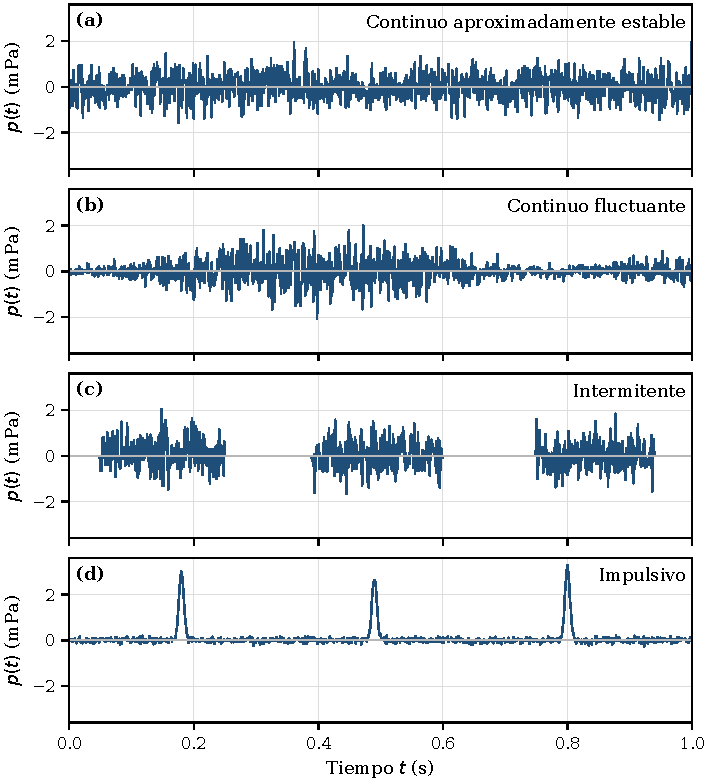
\includegraphics[width=0.96\textwidth]
        {figures/generated/unidad-10/realizaciones-temporales-ruido.pdf}
    \caption{Clasificación temporal mediante cuatro realizaciones sintéticas
    de presión acústica, muestreadas a \(1000\,\mathrm{Hz}\) durante
    \(1\,\mathrm{s}\). Los paneles comparten las escalas de tiempo y presión:
    (a)~continuo aproximadamente estable; (b)~continuo fluctuante;
    (c)~intermitente; y (d)~impulsivo. Las amplitudes ilustran la forma
    temporal y no representan una exposición medida. Elaboración propia con
    semilla fija.}
    \label{fig:u10-realizaciones-temporales}
\end{figure}

\section{Descripción estadística}
\label{sec:u10-estadistica}

Cuando una señal varía, una sola muestra no representa el intervalo completo.
Primero observamos qué pregunta responde cada descriptor y luego introducimos
su expresión matemática.

\subsection{Valor medio, valor eficaz y varianza}

Supongamos que se registran \(N\) muestras de presión acústica
\(p_1,p_2,\ldots,p_N\), todas expresadas en pascales (\(\mathrm{Pa}\)). El
\textbf{valor medio} se define como
\begin{equation}
    \overline{p}=\frac{1}{N}\sum_{i=1}^{N}p_i,
    \label{eq:u10-media}
\end{equation}
donde \(i\) identifica cada muestra. El valor medio conserva el signo. En una
señal acústica alternante medida respecto de la presión atmosférica, los
valores positivos y negativos suelen compensarse, de modo que
\(\overline{p}\) puede ser cercano a \(0\,\mathrm{Pa}\) aunque la señal
transporte energía.

El \textbf{valor eficaz} o RMS cuantifica el tamaño cuadrático de la señal:
\begin{equation}
    p_{\mathrm{rms}}=
    \sqrt{\frac{1}{N}\sum_{i=1}^{N}p_i^2},
    \label{eq:u10-rms}
\end{equation}
donde \(p_{\mathrm{rms}}\) se expresa en pascales (\(\mathrm{Pa}\)). Este valor
es el que se relaciona con el nivel de presión sonora bajo las condiciones
estudiadas en la \nameref{chap:unidad-4}.

La \textbf{varianza} describe la dispersión respecto del valor medio:
\begin{equation}
    \sigma_p^2=
    \frac{1}{N}\sum_{i=1}^{N}\left(p_i-\overline{p}\right)^2,
    \label{eq:u10-varianza}
\end{equation}
donde \(\sigma_p^2\) se expresa en pascales cuadrados
(\(\mathrm{Pa^2}\)). Para estas definiciones,
\begin{equation}
    p_{\mathrm{rms}}^2=\sigma_p^2+\overline{p}^{\,2}.
    \label{eq:u10-identidad-estadistica}
\end{equation}
Por lo tanto, si \(\overline{p}=0\,\mathrm{Pa}\), el cuadrado del valor eficaz
coincide con la varianza, pero los conceptos no son sinónimos.

\paragraph{Ejemplo.}
Consideremos cinco muestras sintéticas:
\(-2,-1,0,1,2\,\mathrm{mPa}\), donde
\(1\,\mathrm{mPa}=10^{-3}\,\mathrm{Pa}\). Su valor medio es
\(0\,\mathrm{mPa}\). El promedio de los cuadrados es
\(2\,\mathrm{mPa^2}\), por lo que
\(p_{\mathrm{rms}}=\sqrt{2}\,\mathrm{mPa}\approx1{,}41\,\mathrm{mPa}\) y
\(\sigma_p^2=2\,\mathrm{mPa^2}\). La media nula no implica ausencia de señal.

\subsection{Distribución e histograma}

La \textbf{distribución} describe con qué frecuencia o probabilidad aparecen
los distintos valores. En un registro finito puede aproximarse mediante un
histograma: se divide el eje de amplitud en intervalos y se cuenta cuántas
muestras caen en cada uno. La distribución aporta información que el RMS no
conserva. Dos señales pueden tener igual valor eficaz y, sin embargo, diferir
en la frecuencia con la que presentan valores extremos.

No debe suponerse que todo ruido posee una distribución normal o gaussiana.
Esa distribución es un modelo posible que debe comprobarse o declararse, no
una consecuencia de llamar ruido a la señal.

La figura~\ref{fig:u10-estadistica-mismo-rms} muestra por qué media, RMS y
varianza no agotan la descripción de una señal: dos registros pueden compartir
esos valores y poseer distribuciones diferentes.

% Texto alternativo: dos señales sintéticas tienen media 0 mPa, RMS 1 mPa y
% varianza 1 mPa². La señal A recorre valores continuos concentrados alrededor
% de cero; la B alterna exclusivamente -1 mPa y +1 mPa. Los histogramas hacen
% visible la diferencia que no expresan los tres descriptores compartidos.
\begin{figure}[htbp]
    \centering
    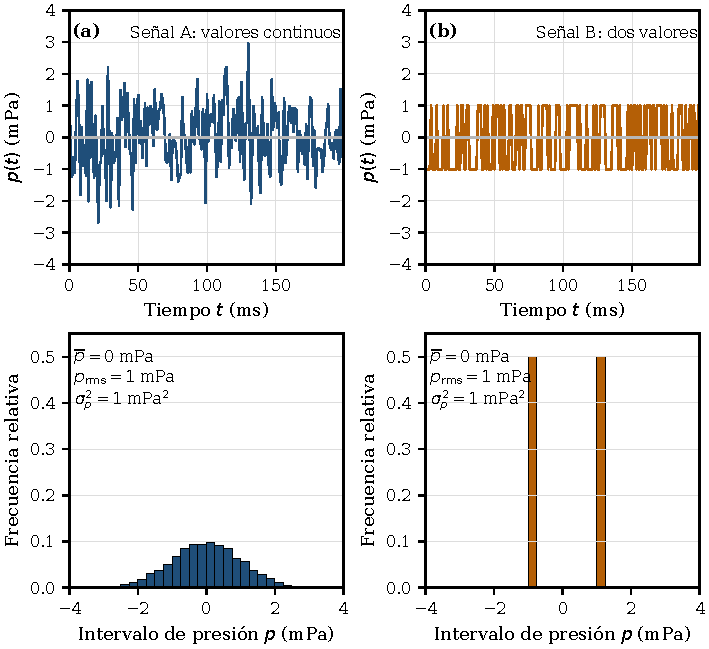
\includegraphics[width=0.96\textwidth]
        {figures/generated/unidad-10/estadistica-mismo-rms.pdf}
    \caption{Fragmentos temporales e histogramas de dos señales sintéticas de
    \(5000\) muestras a \(1000\,\mathrm{Hz}\). Ambas poseen
    \(\overline p=0\,\mathrm{mPa}\),
    \(p_{\mathrm{rms}}=1\,\mathrm{mPa}\) y
    \(\sigma_p^2=1\,\mathrm{mPa^2}\), pero la señal A adopta valores continuos
    y la B solo \(-1\,\mathrm{mPa}\) y \(+1\,\mathrm{mPa}\). El histograma
    utiliza todas las muestras; el registro muestra los primeros
    \(200\,\mathrm{ms}\). Elaboración propia con semilla fija.}
    \label{fig:u10-estadistica-mismo-rms}
\end{figure}

\section{Descripción frecuencial}
\label{sec:u10-densidad-espectral}

El espectro estudiado en la \nameref{chap:unidad-5} permite preguntar cómo
se reparte el contenido de una señal entre frecuencias. Para un proceso
aleatorio resulta útil la \textbf{densidad espectral de potencia de la presión},
que denotaremos \(S_{pp}(f)\). Usaremos una densidad unilateral, definida para
frecuencias no negativas. Aquí \(f\) es la frecuencia, expresada en hertz
(\(\mathrm{Hz}\)), y \(S_{pp}\) se expresa en \(\mathrm{Pa^2/Hz}\).

En el modelo ideal, el valor cuadrático medio contenido entre una frecuencia
inferior \(f_L\) y una frecuencia superior \(f_H\), ambas en hertz, es
\begin{equation}
    p_{B,\mathrm{rms}}^2=
    \int_{f_L}^{f_H}S_{pp}(f)\,\mathrm{d}f,
    \label{eq:u10-psd-banda}
\end{equation}
donde \(p_{B,\mathrm{rms}}\), expresado en pascales, es el valor eficaz de la
señal limitada a esa banda. La densidad no es un nivel en decibeles y tampoco
es, por sí sola, la energía total de una banda: debe integrarse sobre un ancho
de banda.

\paragraph{Ejemplo sintético.}
Si \(S_{pp}(f)=4{,}0\times10^{-8}\,\mathrm{Pa^2/Hz}\) en una banda de
\(100\,\mathrm{Hz}\), entonces
\(p_{B,\mathrm{rms}}^2=4{,}0\times10^{-6}\,\mathrm{Pa^2}\) y
\(p_{B,\mathrm{rms}}=2{,}0\times10^{-3}\,\mathrm{Pa}\). Con la referencia
\(p_0=20\,\mathrm{\mu Pa}\) usada para el aire, ese valor corresponde a
\(L_p=40\,\mathrm{dB\,SPL}\). El ejemplo describe una señal sintética; no es
un límite de exposición.

\subsection{Ruido blanco: densidad constante por hertz}
\label{sec:u10-ruido-blanco}

En un intervalo de frecuencias especificado, un \textbf{ruido blanco} ideal
posee densidad espectral constante:
\begin{equation}
    S_{pp}(f)=S_0,
    \label{eq:u10-blanco}
\end{equation}
donde \(S_0\) es una constante expresada en
\(\mathrm{Pa^2/Hz}\). Por la ecuación~\eqref{eq:u10-psd-banda}, dos bandas con
el mismo ancho en hertz contienen el mismo valor cuadrático medio.

Una octava superior abarca más hertz que una octava inferior. Por eso un ruido
blanco no entrega igual contenido a cada octava. Además, ninguna fuente real
mantiene densidad constante desde frecuencia cero hasta frecuencia infinita:
siempre deben declararse la banda de generación, la banda de medición y las
limitaciones del sistema.

\subsection{Ruido rosa: contenido constante por octava}
\label{sec:u10-ruido-rosa}

En una banda especificada, un \textbf{ruido rosa} ideal se modela mediante
\begin{equation}
    S_{pp}(f)=\frac{K}{f},
    \label{eq:u10-rosa}
\end{equation}
donde \(K\) es una constante con las unidades necesarias para que
\(S_{pp}\) se exprese en \(\mathrm{Pa^2/Hz}\); por lo tanto, \(K\) se expresa
en pascales cuadrados (\(\mathrm{Pa^2}\)). Entre una frecuencia \(f_1\) y
su doble \(2f_1\), que delimitan una octava,
\begin{equation}
    \int_{f_1}^{2f_1}\frac{K}{f}\,\mathrm{d}f=K\ln 2.
    \label{eq:u10-rosa-octava}
\end{equation}
El resultado no depende de \(f_1\): la integral tiene el mismo valor en cada
octava ideal. Esta es la diferencia central. En el modelo blanco la densidad
es constante por hertz. En el modelo rosa, el contenido es constante por
octava. La descripción aproximada de
\(-3\,\mathrm{dB}\) por octava se refiere a la densidad espectral expresada
en escala logarítmica, no a una disminución del nivel total de cada octava.

La figura~\ref{fig:u10-blanco-rosa-bandas} conecta las densidades con la
integral de la ecuación~\eqref{eq:u10-psd-banda}. La diferencia por hertz se
traduce en una diferencia clara al sumar por octavas.

% Texto alternativo: a la izquierda, la densidad blanca es horizontal y la
% rosa decrece como 1/f entre 125 Hz y 8000 Hz. A la derecha, seis grupos de
% barras representan octavas sucesivas: el contenido blanco se duplica en
% cada banda y el rosa permanece constante; ambos se normalizan por la primera.
\begin{figure}[htbp]
    \centering
    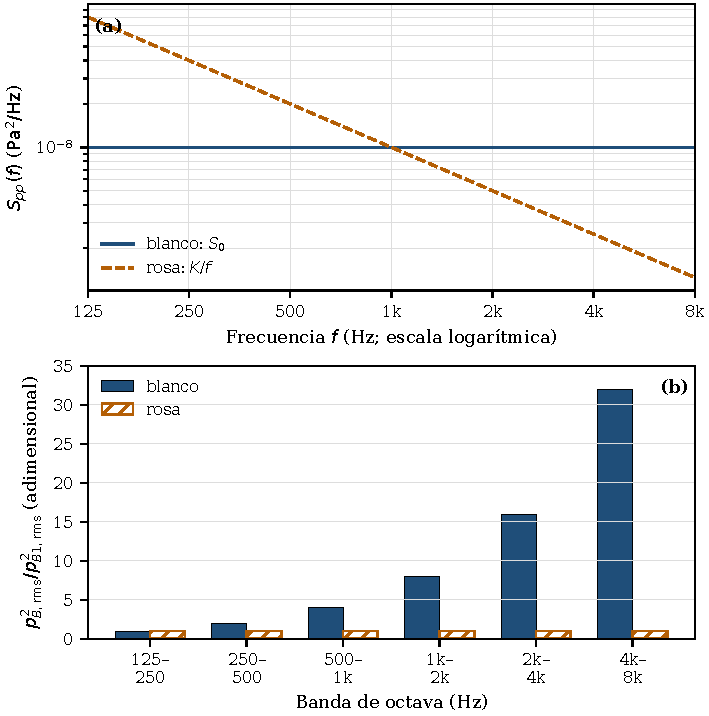
\includegraphics[width=0.98\textwidth]
        {figures/generated/unidad-10/blanco-rosa-energia-bandas.pdf}
    \caption{Modelos analíticos de ruido blanco y rosa en la banda
    \(125\)--\(8000\,\mathrm{Hz}\). (a)~Densidades
    \(S_{pp}(f)=S_0\), con
    \(S_0=1{,}0\times10^{-8}\,\mathrm{Pa^2/Hz}\), y
    \(S_{pp}(f)=K/f\), con \(K=1{,}0\times10^{-5}\,\mathrm{Pa^2}\).
    (b)~Valor cuadrático medio integrado en cada octava y normalizado por la
    primera banda: el blanco aumenta con el ancho en hertz y el rosa permanece
    constante. Son modelos finitos, no mediciones. Elaboración propia.}
    \label{fig:u10-blanco-rosa-bandas}
\end{figure}

\subsection{Ruido con forma espectral vocal}
\label{sec:u10-ruido-vocal}

El \textbf{ruido con forma espectral vocal} es una señal aleatoria filtrada
para aproximar una distribución frecuencial de referencia asociada con el
habla. No existe una única forma que pueda deducirse de su nombre: deben
especificarse el espectro objetivo, el ancho de banda, el nivel y el equipo que
lo genera.

Las denominaciones, tolerancias y usos audiométricos de los ruidos con
forma espectral vocal dependen de la norma, del transductor, del audiómetro y
del procedimiento aplicable. Una fuente normativa o documentación técnica
vigente debe acompañar cualquier especificación cuantitativa~\cite{iso389_4_1994,iec60645_1_2017}.

\subsection{Ruido de banda estrecha}
\label{sec:u10-nbn}

Un \textbf{ruido de banda estrecha} o NBN, por la sigla inglesa de
\emph{narrow-band noise}, concentra su contenido alrededor de una frecuencia
central \(f_c\), expresada en hertz. Para caracterizarlo se deben declarar la
frecuencia límite inferior \(f_L\), la frecuencia límite superior \(f_H\) y el
ancho de banda
\begin{equation}
    B=f_H-f_L,
    \label{eq:u10-ancho-nbn}
\end{equation}
donde \(B\) se expresa en hertz. También importa la pendiente del filtro fuera
de la banda. ``Banda estrecha'' no significa universalmente un tercio de
octava.

En audiometría tonal pueden emplearse ruidos de banda estrecha como
señales enmascarantes, pero sus bandas efectivas, calibración y presentación
deben corresponder al equipo, al transductor y al procedimiento vigente~\cite{iso389_4_1994,iec60645_1_2017}.

En el esquema siguiente, \(H_v(f)\) es la respuesta en frecuencia del filtro
que produce el ruido con forma espectral vocal y \(H_B(f)\) la del filtro que
produce el NBN. Se representan sus magnitudes adimensionales
\(\lvert H_v(f)\rvert\) y \(\lvert H_B(f)\rvert\) de manera cualitativa: las
curvas muestran una forma relativa, no una ganancia ni un nivel calibrados.
La figura~\ref{fig:u10-conformacion-espectral} resume qué transforma a un
ruido de banda ancha en cada una de estas señales y qué información debe
acompañar su nombre.

% Texto alternativo: dos cadenas parten de ruido de banda ancha. La superior
% atraviesa un filtro con respuesta objetivo especificada y produce ruido con
% forma espectral vocal. La inferior atraviesa un pasa banda delimitado por
% f_L y f_H, centrado en f_c, y produce ruido de banda estrecha.
\begin{figure}[htbp]
    \centering
    % Propósito: distinguir una conformación espectral de referencia de una banda
% estrecha y mostrar qué parámetros deben especificarse en cada caso.
% Origen: definiciones de las secciones \ref{sec:u10-ruido-vocal} y
% \ref{sec:u10-nbn}; B=f_H-f_L, ecuación \eqref{eq:u10-ancho-nbn}.
% Curvas y bloques cualitativos; no representan una norma ni un equipo.
% Descripción accesible: dos cadenas parten de ruido de banda ancha. La cadena
% superior atraviesa un filtro cuya respuesta H_v(f) posee una magnitud
% objetivo especificada y produce ruido con forma espectral vocal. La inferior
% atraviesa un filtro pasa banda de respuesta H_B(f), delimitado por f_L y
% f_H, centrado en f_c, y produce NBN.
\begin{tikzpicture}[
    x=0.95cm,
    y=1cm,
    >=stealth,
    font=\small,
    bloque/.style={
        draw,
        rounded corners,
        minimum width=2.55cm,
        minimum height=1.05cm,
        align=center,
        fill=black!3
    },
    filtro/.style={
        draw,
        minimum width=3.50cm,
        minimum height=1.45cm,
        align=center,
        fill=black!8
    },
    salida/.style={
        draw,
        rounded corners,
        minimum width=2.80cm,
        minimum height=1.05cm,
        align=center,
        very thick
    }
]
    \node[bloque] (entrada-v) at (1.55,4.65)
        {ruido de\\banda ancha};
    \node[filtro] (filtro-v) at (6.00,4.65)
        {\(\lvert H_v(f)\rvert\)\\
         respuesta objetivo\\especificada};
    \node[salida] (salida-v) at (10.55,4.65)
        {ruido con forma\\espectral vocal};
    \draw[->,very thick] (entrada-v) -- (filtro-v);
    \draw[->,very thick] (filtro-v) -- (salida-v);

    \node[align=center,font=\footnotesize,text width=8.4cm]
        at (6.00,3.55)
        {declarar espectro objetivo, banda, nivel, equipo y procedimiento};

    \node[bloque] (entrada-b) at (1.55,1.90)
        {ruido de\\banda ancha};
    \node[filtro,minimum height=2.05cm] (filtro-b) at (6.00,1.90) {};
    \node[salida] (salida-b) at (10.55,1.90)
        {ruido de banda\\estrecha (NBN)};
    \draw[->,very thick] (entrada-b) -- (filtro-b);
    \draw[->,very thick] (filtro-b) -- (salida-b);

    \begin{scope}[shift={(4.55,1.48)},x=0.72cm,y=0.62cm]
        \draw[->] (0,0) -- (4.00,0);
        \node[font=\footnotesize] at (3.38,1.43)
            {\(f\) (Hz)};
        \draw[->] (0,0) -- (0,1.55);
        \node[below right,font=\footnotesize] at (0,1.55)
            {\(\lvert H_B(f)\rvert\)};
        \draw[very thick]
            (0.15,0.08) -- (0.95,0.08) -- (1.35,1.25) --
            (2.55,1.25) -- (2.95,0.08) -- (3.80,0.08);
        \draw[densely dotted] (1.35,0) -- (1.35,1.25);
        \draw[densely dotted] (1.95,0) -- (1.95,1.25);
        \draw[densely dotted] (2.55,0) -- (2.55,1.25);
        \node[below=1pt,font=\footnotesize] at (1.35,0) {\(f_L\)};
        \node[below=1pt,font=\footnotesize] at (1.95,0) {\(f_c\)};
        \node[below=1pt,font=\footnotesize] at (2.55,0) {\(f_H\)};
    \end{scope}

    \node[align=center,font=\footnotesize,text width=10.0cm]
        at (6.00,0.46)
        {parámetros: \(f_L,\ f_c,\ f_H,\ B=f_H-f_L\);\\[-1pt]
         pendientes, nivel y calibración};
\end{tikzpicture}

    \caption{Conformación espectral de dos señales de ruido.
    En la cadena superior, \(\lvert H_v(f)\rvert\) representa la magnitud de la
    respuesta objetivo que produce el ruido con forma espectral vocal; el
    nombre no define una curva universal. En la inferior,
    \(\lvert H_B(f)\rvert\) representa la magnitud de la respuesta pasa banda
    que produce el NBN, para el cual deben declararse \(f_L\), \(f_c\), \(f_H\),
    el ancho \(B=f_H-f_L\), las pendientes, el nivel y la calibración. Esquema
    cualitativo de elaboración propia; no reproduce una norma ni un equipo.}
    \label{fig:u10-conformacion-espectral}
\end{figure}

\section{Descriptores temporales y métricas de exposición}
\label{sec:u10-metricas}

Una lectura de nivel solo es interpretable si se informa qué operación se
realizó, con qué ponderación frecuencial y durante qué intervalo. La
instrumentación básica y las ponderaciones A, C y Z se estudiaron en la
\nameref{chap:unidad-5}. Aquí comparamos las preguntas que responden los
descriptores más frecuentes.

En la tabla, todos los niveles se expresan en decibeles (\(\mathrm{dB}\)) con
el calificador que corresponda, por ejemplo \(\mathrm{dB(A)}\) o
\(\mathrm{dB\,SPL}\).

\begin{center}
\small
\begin{tabular}{|
    >{\raggedright\arraybackslash}p{0.22\textwidth}|
    >{\raggedright\arraybackslash}p{0.32\textwidth}|
    >{\raggedright\arraybackslash}p{0.34\textwidth}|}
    \hline
    \textbf{Descriptor} & \textbf{Qué representa} &
    \textbf{Qué debe acompañarlo} \\
    \hline
    \(L(t)\) & Nivel indicado en un instante por el detector elegido. &
    Ponderación frecuencial y respuesta temporal. \\
    \hline
    \(L_{\mathrm{max}}\) & Mayor nivel indicado durante el intervalo. &
    Ponderaciones frecuencial y temporal e intervalo de búsqueda. \\
    \hline
    \(L_{\mathrm{peak}}\) & Nivel asociado con el mayor valor absoluto
    instantáneo de presión captado por un detector de pico. &
    Ponderación frecuencial, rango del equipo y procedimiento. \\
    \hline
    \(L_{\mathrm{eq},T}\) & Nivel constante que posee el mismo promedio
    cuadrático que la señal variable durante \(T\). &
    Duración \(T\), ponderación frecuencial y condiciones de medición. \\
    \hline
    \(L_{n,T}\) & Nivel excedido durante el \(n\)~\% del intervalo \(T\). &
    Valor de \(n\), duración, ponderación y criterio de muestreo. \\
    \hline
    Exposición o dosis & Agregación de nivel y duración para compararla con
    un criterio. & Norma, edición, jurisdicción, población y regla de
    intercambio. \\
    \hline
\end{tabular}
\end{center}

El nivel máximo no es necesariamente el nivel de pico. El primero depende de
la respuesta temporal del instrumento; el segundo intenta representar un
extremo de la presión instantánea. La ponderación temporal \emph{Impulse}
tampoco convierte automáticamente una lectura en \(L_{\mathrm{peak}}\).

El nivel equivalente no es un promedio aritmético de niveles en decibeles. Si
se dispone de \(M\) intervalos de igual duración con niveles equivalentes
\(L_1,L_2,\ldots,L_M\), todos expresados con la misma referencia y
ponderación, se obtiene
\begin{equation}
    L_{\mathrm{eq}}=
    10\log_{10}\left(
    \frac{1}{M}\sum_{j=1}^{M}10^{L_j/10}
    \right),
    \label{eq:u10-leq-intervalos}
\end{equation}
donde \(j\) identifica cada intervalo.

\paragraph{Ejemplo.}
Cuatro intervalos consecutivos de \(15\,\mathrm{min}\) poseen niveles
equivalentes ponderados A de \(88\), \(92\), \(86\) y \(90\,\mathrm{dB(A)}\).
Como las duraciones son iguales,
\[
L_{A\mathrm{eq},1\,\mathrm{h}}=
10\log_{10}\left(
\frac{10^{88/10}+10^{92/10}+10^{86/10}+10^{90/10}}{4}
\right)
\approx89{,}6\,\mathrm{dB(A)}.
\]
El resultado resume el promedio cuadrático ponderado A durante una hora; no
informa por sí solo el máximo ni el pico.

Los percentiles tampoco poseen una interpretación universal. En
\(L_{n,T}\), el subíndice \(n\) representa el porcentaje de excedencia y no es
una abreviatura de ruido. \(L_{10,T}\) es el nivel excedido durante el
\(10\)~\% de \(T\), y
\(L_{90,T}\), el excedido durante el \(90\)~\%. En algunos contextos el
segundo se usa como descriptor del ambiente residual, pero no debe llamarse
automáticamente ``ruido de fondo'' sin definir el procedimiento.

La normalización de una exposición a una jornada de referencia, el
cálculo de dosis y la combinación de protección auditiva dependen del criterio
normativo vigente. No deben mezclarse valores procedentes de organismos,
ediciones o jurisdicciones diferentes~\cite{nioshNoise1998,argentinaDecreto351}.

\section{Relación señal--ruido y ruido de fondo}
\label{sec:u10-snr-fondo}

La \textbf{señal de interés} es la componente que se intenta detectar, medir o
comprender. El \textbf{ruido de fondo} reúne las componentes no deseadas
presentes en el entorno o en la cadena de medición. En cambio, una
\textbf{señal enmascarante} se introduce deliberadamente para modificar la
detectabilidad de otra señal. Un mismo tipo espectral puede cumplir funciones
diferentes según cómo se lo utilice.

Para niveles compatibles y medidos en condiciones comparables, una forma
simple de expresar la relación señal--ruido es
\begin{equation}
    \mathrm{SNR}=L_{\text{señal}}-L_{\text{ruido}},
    \label{eq:u10-snr}
\end{equation}
donde \(L_{\text{señal}}\) es el nivel de la señal,
\(L_{\text{ruido}}\) el nivel del ruido y la SNR se expresa en decibeles
(\(\mathrm{dB}\)). Por ejemplo, si
\(L_{\text{señal}}=65\,\mathrm{dB\,SPL}\) y
\(L_{\text{ruido}}=58\,\mathrm{dB\,SPL}\), ambos medidos en la misma banda y
posición, entonces \(\mathrm{SNR}=7\,\mathrm{dB}\).

La SNR física no es una medida directa de inteligibilidad, molestia ni
esfuerzo auditivo. Esos resultados dependen además del espectro, el tiempo, el
entorno, la tarea y el oyente, como se analizó en la
\nameref{chap:unidad-7}.

La figura~\ref{fig:u10-snr-sintetica} mantiene fija la señal de interés y
modifica solo el RMS del ruido. Así se observa qué significa reducir la SNR
sin convertirla en una predicción perceptual.

% Texto alternativo: tres mezclas contienen la misma señal sintética y la misma
% realización de ruido, escalada para SNR de +12 dB, 0 dB y -6 dB. La mezcla
% sigue de cerca la señal limpia en el primer panel y se aparta cada vez más
% en los dos siguientes.
\begin{figure}[htbp]
    \centering
    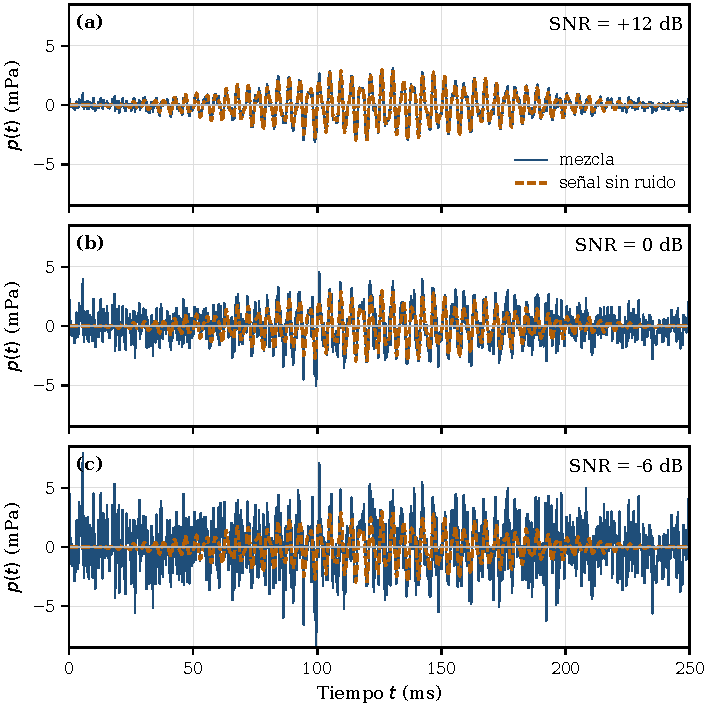
\includegraphics[width=0.96\textwidth]
        {figures/generated/unidad-10/relaciones-senal-ruido.pdf}
    \caption{Una señal sintética de \(250\,\mathrm{ms}\), formada por
    componentes de \(240\,\mathrm{Hz}\) y \(430\,\mathrm{Hz}\) bajo una
    envolvente suave, se suma a la misma realización de ruido con tres escalas:
    (a)~\(\mathrm{SNR}=+12\,\mathrm{dB}\);
    (b)~\(\mathrm{SNR}=0\,\mathrm{dB}\); y
    (c)~\(\mathrm{SNR}=-6\,\mathrm{dB}\). La señal posee
    \(p_{\mathrm{rms}}=1\,\mathrm{mPa}\); el ruido se ajusta por RMS para
    alcanzar cada relación. No son registros de habla ni mediciones.
    Elaboración propia con semilla fija.}
    \label{fig:u10-snr-sintetica}
\end{figure}

\section{Enmascaramiento: del fenómeno perceptual a la aplicación}
\label{sec:u10-enmascaramiento-aplicado}

El enmascaramiento es la disminución de detectabilidad de una señal debido a
otra. La elevación de umbral, las bandas auditivas y las dependencias
frecuencial y temporal pertenecen a la \nameref{chap:unidad-7}. En esta
unidad nos concentramos en describir la señal utilizada como enmascarante.

En una situación controlada conviene identificar:
\begin{enumerate}
    \item la \textbf{señal de prueba};
    \item el \textbf{enmascarante}, con su espectro, banda y nivel;
    \item el \textbf{canal o receptor} al que se presenta cada señal; y
    \item la \textbf{respuesta} que se observa.
\end{enumerate}

En audiometría, el enmascaramiento puede utilizarse para reducir la
contribución del oído no evaluado cuando existe posibilidad de respuesta
cruzada. La decisión de enmascarar, la elección del transductor, los niveles,
los incrementos y los criterios de finalización pertenecen a un protocolo
audiológico vigente y no se deducen solo del tipo de ruido~\cite{ashaPureTone2005}.

La figura~\ref{fig:u10-enmascaramiento-audiometrico} muestra la función de cada
señal sin indicar niveles. No debe transformarse en una receta. En particular,
\textbf{enmascaramiento clínico} y \textbf{protección auditiva} no son
sinónimos: el primero manipula de manera controlada la detectabilidad durante
una prueba; la segunda busca reducir la exposición que alcanza el receptor.

% Texto alternativo: la señal de prueba llega al oído evaluado y, mediante una
% posible ruta cruzada discontinua, al oído no evaluado. Un enmascarante
% controlado se presenta al oído no evaluado para disminuir allí la
% detectabilidad de la señal cruzada. No aparecen niveles ni incrementos.
\begin{figure}[htbp]
    \centering
    % Propósito: mostrar por qué el enmascarante se presenta al oído no evaluado
% cuando una señal de prueba podría producir una respuesta cruzada.
% Origen: sección \ref{sec:u10-enmascaramiento-aplicado}; esquema funcional
% cualitativo, sin niveles, incrementos ni criterio clínico.
% Descripción accesible: la señal de prueba llega por una ruta directa al oído
% evaluado y por una ruta cruzada discontinua al oído no evaluado. Un
% enmascarante controlado llega al oído no evaluado y reduce allí la
% detectabilidad de la señal cruzada. La respuesta observada no identifica por
% sí sola qué oído detectó la señal.
\begin{tikzpicture}[
    x=0.965cm,
    y=1cm,
    >=stealth,
    font=\small,
    senal/.style={
        draw,
        rounded corners,
        minimum width=2.65cm,
        minimum height=0.95cm,
        align=center,
        fill=black!3
    },
    oido/.style={
        draw,
        very thick,
        rounded corners,
        minimum width=2.85cm,
        minimum height=1.15cm,
        align=center
    },
    resultado/.style={
        draw,
        rounded corners,
        minimum width=3.25cm,
        minimum height=1.05cm,
        align=center,
        font=\footnotesize
    }
]
    \node[senal] (prueba) at (1.70,4.25)
        {señal de prueba};
    \node[senal] (masker) at (1.70,1.35)
        {enmascarante\\presentado deliberadamente};

    \node[oido] (evaluado) at (6.00,4.25)
        {\textbf{oído evaluado}\\
         canal de interés};
    \node[oido] (no-evaluado) at (6.00,1.35)
        {\textbf{oído no evaluado}\\
         canal que se controla};

    \node[resultado] (deteccion) at (10.40,4.25)
        {detección atribuible\\
         al canal de interés};
    \node[resultado] (cruzada) at (10.40,1.35)
        {menor detectabilidad\\
         de la señal cruzada};

    \draw[->,very thick] (prueba) -- (evaluado);
    \draw[->,very thick] (evaluado) -- (deteccion);

    \draw[->,very thick,dashed]
        (prueba.south east)
        .. controls (3.50,3.25) and (4.10,2.15) ..
        (no-evaluado.north west);
    \node[
        fill=white,
        inner sep=1.5pt,
        align=center,
        font=\footnotesize
    ] at (3.72,2.85)
        {posible ruta\\cruzada};

    \draw[->,very thick] (masker) -- (no-evaluado);
    \draw[->,very thick] (no-evaluado) -- (cruzada);

    \node[
        draw,
        rounded corners,
        fill=black!5,
        align=center,
        font=\footnotesize,
        text width=8.9cm
    ] at (6.05,-0.05)
        {Esquema conceptual: no prescribe niveles ni reemplaza un protocolo.
         La respuesta observada debe interpretarse según la prueba.};
\end{tikzpicture}

    \caption{Esquema funcional del enmascaramiento audiométrico introductorio.
    La señal de prueba se dirige al oído evaluado, pero puede existir una ruta
    cruzada hacia el oído no evaluado. El enmascarante se presenta de manera
    deliberada en este último para disminuir allí la detectabilidad de la
    señal cruzada. La figura no establece indicaciones, niveles, incrementos
    ni criterios de finalización. Elaboración propia.}
    \label{fig:u10-enmascaramiento-audiometrico}
\end{figure}

La acufenometría puede incluir la comparación de tonos o ruidos con la
percepción referida por la persona y la determinación de medidas de
enmascaramiento. Su interpretación y el uso terapéutico de sonidos requieren
evaluación profesional, protocolo y evidencia clínica específica. Esta unidad
no prescribe un tipo de ruido ni un nivel para tinnitus~\cite{ashaTinnitus}.

\section{Exposición, salud y comunicación}
\label{sec:u10-efectos}

El ruido puede estudiarse en tres planos que conviene mantener separados:
\begin{description}
    \item[\textbf{Exposición física:}] nivel, espectro, duración, repetición y
    condiciones de propagación.
    \item[\textbf{Resultado funcional o perceptual:}] detectabilidad,
    inteligibilidad, molestia, esfuerzo o interferencia con una tarea.
    \item[\textbf{Resultado de salud:}] alteración, síntoma o riesgo evaluado
    en una población y bajo condiciones definidas.
\end{description}

La exposición a determinados niveles y duraciones puede asociarse con
efectos auditivos, como cambios temporales o permanentes de umbral y tinnitus,
y con efectos no auditivos. La magnitud del riesgo depende de la exposición y
de factores individuales y contextuales; una medición aislada no establece
por sí sola un diagnóstico ni una relación causal individual~\cite{whoEnvNoise2018,nioshNoise1998}.

El ruido puede interferir con la comunicación oral y con tareas que
requieren atención. El resultado depende, entre otros factores, de la SNR, el
contenido espectral y temporal, la reverberación, la distancia, las
características del habla, la tarea y el oyente~\cite{whoEnvNoise2018,nioshNoise1998}.

Las alteraciones, los estudios y la rehabilitación se desarrollaron en la
\nameref{chap:unidad-8}. Esta unidad aporta descriptores de la exposición,
pero no reemplaza una evaluación clínica ni ofrece consejo médico individual.

\subsection{Cómo leer recomendaciones y normas}
\label{sec:u10-normativa}

No todo documento que contiene decibeles cumple la misma función:
\begin{center}
\begin{tabular}{|
    >{\raggedright\arraybackslash}p{0.24\textwidth}|
    >{\raggedright\arraybackslash}p{0.31\textwidth}|
    >{\raggedright\arraybackslash}p{0.33\textwidth}|}
    \hline
    \textbf{Tipo de documento} & \textbf{Pregunta principal} &
    \textbf{Dato imprescindible} \\
    \hline
    Norma de medición & ¿Cómo medir, calcular e informar una magnitud? &
    Edición, instrumento, ponderaciones, intervalo y procedimiento. \\
    \hline
    Guía de salud & ¿Qué asociación o recomendación se propone para una
    población y un resultado? &
    Organismo, población, indicador, evidencia y alcance. \\
    \hline
    Criterio legal u ocupacional & ¿Qué obligación o acción corresponde en
    una jurisdicción? &
    Autoridad, jurisdicción, vigencia, jornada, regla de intercambio y
    excepciones. \\
    \hline
\end{tabular}
\end{center}

Por lo tanto, no se debe atribuir a una norma de medición un límite sanitario
que no establece, ni combinar el nivel admisible de un documento con la regla
de intercambio de otro.

Antes de aplicar recomendaciones de exposición o seleccionar
protección auditiva deben consultarse las normas técnicas, la legislación y
las guías vigentes para la jurisdicción y la población correspondientes. En
Argentina, cualquier referencia ocupacional debe comprobarse en las fuentes
oficiales actuales y no trasladarse automáticamente a ambientes comunitarios,
educativos o clínicos~\cite{argentinaLey19587,argentinaDecreto351,argentinaResolucion85}.

Los límites de ruido admisible para salas de prueba audiométrica
dependen de la prueba, la vía, el transductor, las frecuencias evaluadas y el
documento técnico aplicable. Un único valor global en \(\mathrm{dB(A)}\) no
garantiza por sí solo que una cabina sea adecuada~\cite{iso8253_1_2010,ansiS31_2023}. Véase también la
sección~\ref{sec:u9-ruido-cabina}.

\section{Control en la fuente, el trayecto y el receptor}
\label{sec:u10-control}

Controlar ruido significa modificar una cadena física para reducir la
exposición o la interferencia relevante. Conviene comenzar por identificar la
fuente, seguir el trayecto de transmisión y definir el receptor o la tarea que
se desea proteger.

\begin{description}
    \item[\textbf{Fuente:}] reducir la generación mediante selección,
    mantenimiento, ajuste de operación, encapsulado o sustitución del proceso,
    según el caso.
    \item[\textbf{Trayecto:}] aumentar distancia, interponer cerramientos o
    barreras, controlar aberturas, desacoplar vibraciones o acondicionar el
    recinto cuando corresponda.
    \item[\textbf{Receptor:}] limitar el tiempo de exposición, organizar la
    tarea, alejar al receptor o emplear protección auditiva seleccionada y
    verificada para la situación.
\end{description}

Las jerarquías de control ocupacional suelen priorizar la eliminación
o reducción en la fuente y las medidas de ingeniería antes que las medidas
administrativas y la protección personal. La formulación exacta debe
verificarse en el marco normativo vigente~\cite{nioshHierarchy2024}.

La figura~\ref{fig:u10-control-ftr} organiza las medidas según el eslabón sobre
el que actúan. La reducción es el resultado comparado; absorción, aislamiento,
cancelación activa y protección describen mecanismos o intervenciones.

% Texto alternativo: una cadena horizontal conecta fuente, trayecto y receptor.
% Bajo la fuente aparecen acciones sobre la generación; bajo el trayecto se
% separan transmisión y reflexiones; bajo el receptor aparecen distancia,
% tiempo, organización y protección. Las tres familias de acciones apuntan a
% un bloque común que presenta la reducción como resultado comparado entre
% condiciones.
\begin{figure}[htbp]
    \centering
    % Propósito: organizar las medidas de control según el eslabón físico sobre el
% que actúan y separar transmisión, reflexión y protección.
% Origen: sección \ref{sec:u10-control}; esquema cualitativo sin prestaciones.
% Descripción accesible: una cadena conecta fuente, trayecto y receptor. Debajo
% de la fuente aparecen reducción de generación y encapsulado; debajo del
% trayecto se separan transmisión y reflexiones; debajo del receptor aparecen
% distancia, tiempo, organización y protección. Las tres familias de acciones
% apuntan a un bloque común: el resultado se evalúa como cambio de una métrica
% entre condiciones declaradas.
\begin{tikzpicture}[
    x=1cm,
    y=1cm,
    >=stealth,
    font=\small,
    etapa/.style={
        draw,
        rounded corners,
        very thick,
        minimum width=3.15cm,
        minimum height=1.05cm,
        align=center,
        fill=black!4
    },
    accion/.style={
        draw,
        rounded corners,
        minimum width=3.15cm,
        minimum height=1.35cm,
        align=center,
        font=\footnotesize
    },
    resultado/.style={
        draw,
        rounded corners,
        minimum width=9.20cm,
        minimum height=0.85cm,
        align=center,
        fill=black!5,
        font=\footnotesize
    }
]
    \node[etapa] (fuente) at (1.90,4.25)
        {\textbf{Fuente}\\¿dónde se genera?};
    \node[etapa] (trayecto) at (6.10,4.25)
        {\textbf{Trayecto}\\¿cómo se transmite?};
    \node[etapa] (receptor) at (10.30,4.25)
        {\textbf{Receptor}\\¿qué se protege?};

    \draw[->,very thick] (fuente) -- (trayecto)
        node[midway,above=23pt,font=\footnotesize] {propagación};
    \draw[->,very thick] (trayecto) -- (receptor)
        node[midway,above=23pt,font=\footnotesize] {exposición};

    \node[accion] (accion-f) at (1.90,2.15)
        {reducir generación\\
         mantenimiento o sustitución\\
         encapsulado de la fuente};
    \node[accion] (accion-t) at (6.10,2.15)
        {\textbf{transmisión:} barrera,\\
         cerramiento o sellado\\[2pt]
         \textbf{reflexiones:} absorción\\
         y acondicionamiento};
    \node[accion] (accion-r) at (10.30,2.15)
        {distancia y tiempo\\
         organización de la tarea\\
         protección seleccionada};

    \draw[->,thick] (fuente) -- (accion-f);
    \draw[->,thick] (trayecto) -- (accion-t);
    \draw[->,thick] (receptor) -- (accion-r);

    \node[resultado] (resultado) at (6.10,0.48)
        {\textbf{Resultado comprobado:} reducción de una métrica de ruido\\
         entre condiciones declaradas};
    \draw[->,thick] (accion-f.south) -- (1.90,0.91);
    \draw[->,thick] (accion-t.south) -- (6.10,0.91);
    \draw[->,thick] (accion-r.south) -- (10.30,0.91);
\end{tikzpicture}

    \caption{Mapa de control en la cadena fuente--trayecto--receptor. Las
    acciones sobre la fuente modifican la generación; las del trayecto actúan
    sobre transmisión o reflexiones; y las del receptor modifican la
    exposición o la tarea. ``Reducción de ruido'' designa el cambio de una
    métrica entre condiciones declaradas, no un mecanismo único. Esquema
    cualitativo de elaboración propia.}
    \label{fig:u10-control-ftr}
\end{figure}

\subsection{Términos que no deben confundirse}

\begin{description}
    \item[\textbf{Reducción de ruido:}] resultado general: disminución de una
    métrica de ruido entre dos condiciones declaradas.
    \item[\textbf{Absorción:}] disminución de la energía reflejada por una
    superficie; puede modificar la reverberación, pero no equivale a aislar.
    \item[\textbf{Aislamiento:}] reducción de la transmisión entre recintos o
    a través de un elemento constructivo.
    \item[\textbf{Cancelación activa:}] superposición controlada de una señal
    secundaria para reducir la presión en una región y bajo condiciones
    específicas; no elimina universalmente el campo sonoro.
    \item[\textbf{Protección auditiva:}] dispositivo y programa
    destinados a reducir la exposición que llega al oído. Su desempeño real
    no se obtiene sumando sin más valores declarados por fabricantes; la
    selección y la estimación de la protección requieren el procedimiento
    vigente~\cite{iso4869_2_2018}.
\end{description}

Los principios de absorción, transmisión, aislamiento y cabinas se
desarrollaron en la \nameref{chap:unidad-9}. La cancelación activa se apoya
en la superposición estudiada en la \nameref{chap:unidad-3}.

\paragraph{Ejemplo de reducción.}
Sean \(I_i\) la intensidad inicial e \(I_f\) la intensidad final, ambas
expresadas en vatios por metro cuadrado (\(\mathrm{W/m^2}\)). Sean \(L_i\) y
\(L_f\) sus niveles de intensidad asociados, expresados en decibeles y
calculados respecto de una misma intensidad de referencia. Si
\(I_f=0{,}1I_i\), el cambio de nivel es
\[
L_f-L_i
=10\log_{10}\left(\frac{I_f}{I_i}\right)
=10\log_{10}(0{,}1)=-10\,\mathrm{dB}.
\]
Si definimos la reducción positiva como
\(R=L_i-L_f\), entonces
\(R=10\,\mathrm{dB}\). Debe declararse dónde se midió cada intensidad y qué
otras condiciones se mantuvieron constantes.

\section{Relación con la Fonoaudiología}
\label{sec:u10-fonoaudiologia}

La caracterización del ruido permite formular preguntas relevantes sin saltar
directamente a conclusiones clínicas:
\begin{itemize}
    \item en una evaluación auditiva, ayuda a describir el ambiente y las
    señales de prueba;
    \item en voz y habla, permite analizar la SNR y la interferencia con la
    comunicación;
    \item en salud ocupacional y comunitaria, permite describir la exposición
    con la métrica elegida; y
    \item en el diseño de espacios, orienta la elección entre actuar sobre la
    fuente, el trayecto o el receptor.
\end{itemize}

La contribución fonoaudiológica no consiste en reemplazar la medición técnica,
la normativa o el diagnóstico por una impresión general. Consiste en conectar
las propiedades físicas de la señal con la tarea comunicativa o auditiva,
reconociendo los límites de cada inferencia.

\section{Errores frecuentes}
\label{sec:u10-errores}

\begin{itemize}
    \item \textbf{``Ruido'' significa siempre sonido intenso.} No. Puede
    tratarse de una señal de bajo nivel que interfiere con una tarea.
    \item \textbf{Aleatorio significa no medible.} No. No se predice cada
    muestra, pero se describen propiedades estadísticas y espectrales.
    \item \textbf{Estacionario significa constante muestra a muestra.} No.
    Pueden variar los valores instantáneos mientras ciertas estadísticas
    permanecen estables.
    \item \textbf{Media y RMS son equivalentes.} No. La media conserva el
    signo; el RMS se obtiene a partir de cuadrados.
    \item \textbf{Ruido blanco significa igual energía por octava.} No. Posee
    densidad constante por hertz; el rosa ideal posee contenido constante por
    octava.
    \item \textbf{\(L_{\mathrm{max}}\) y \(L_{\mathrm{peak}}\) son
    intercambiables.} No. Dependen de detectores distintos.
    \item \textbf{\(L_{\mathrm{eq}}\) es el promedio aritmético de los
    decibeles.} No. Se promedian primero cantidades lineales proporcionales al
    valor cuadrático.
    \item \textbf{\(L_{90}\) siempre es el ruido de fondo.} No. Es un
    percentil; su uso como descriptor de fondo depende del contexto.
    \item \textbf{Enmascarar equivale a proteger el oído.} No. Son objetivos y
    procedimientos diferentes.
    \item \textbf{Absorber equivale a aislar.} No. La absorción modifica
    reflexiones; el aislamiento limita transmisión entre espacios.
    \item \textbf{Un número en \(\mathrm{dB(A)}\) basta para decidir
    cumplimiento o riesgo.} No. Faltan duración, procedimiento, norma,
    población y jurisdicción.
\end{itemize}

\section{Síntesis}
\label{sec:u10-sintesis}

\begin{itemize}
    \item El sonido es un fenómeno físico; ruido es una categoría que puede
    referirse a una valoración contextual, una componente no deseada o una
    señal de ensayo.
    \item Las señales determinísticas se predicen a partir de un modelo; las
    aleatorias se describen mediante realizaciones y estadísticas.
    \item Estacionariedad y clasificación temporal dependen del intervalo de
    observación. Continuo, fluctuante, intermitente e impulsivo describen
    aspectos distintos.
    \item El valor medio, el RMS, la varianza y la distribución responden
    preguntas diferentes.
    \item La densidad espectral \(S_{pp}(f)\), en
    \(\mathrm{Pa^2/Hz}\), se integra sobre una banda para obtener presión
    cuadrática media.
    \item El ruido blanco posee densidad constante por hertz; el rosa ideal,
    contenido constante por octava.
    \item Los ruidos con forma espectral vocal y de banda estrecha deben
    definirse mediante espectro, límites, ancho de banda y nivel, no solo por
    su nombre.
    \item Nivel instantáneo, máximo, de pico y equivalente no son
    intercambiables.
    \item El ruido de fondo aparece como interferencia; un enmascarante se
    presenta deliberadamente. Ninguno equivale por sí mismo a protección
    auditiva.
    \item Las recomendaciones de exposición y protección requieren fuentes
    vigentes y no constituyen consejo médico individual.
    \item El control se organiza en fuente, trayecto y receptor, diferenciando
    reducción, absorción, aislamiento, cancelación activa y protección.
\end{itemize}

\section{Ejercicios y autoevaluación}
\label{sec:u10-ejercicios}

\subsection*{Preguntas conceptuales}

\begin{enumerate}[label=\textbf{C\arabic*.},leftmargin=*]
    \item Explique por qué una misma señal puede ser sonido para quien desea
    escucharla y ruido respecto de otra tarea, sin que cambien sus propiedades
    físicas.
    \item Compare una sinusoide ideal cuyos parámetros son conocidos con un
    registro aleatorio de tránsito. Indique qué puede predecirse en cada
    instante y qué debe describirse mediante propiedades estadísticas.
    \item ¿Puede una señal estacionaria cambiar muestra a muestra? Explique
    por qué la respuesta depende también del intervalo de observación.
    \item Distinga ruido continuo, fluctuante, intermitente e impulsivo.
    Explique por qué estas categorías no son necesariamente excluyentes.
    \item Diferencie valor medio, valor eficaz o RMS y varianza. Indique sus
    unidades para una señal de presión acústica expresada en pascales
    \((\mathrm{Pa})\).
    \item ¿Qué información aporta la distribución de amplitudes que no aporta
    por sí solo el RMS?
    \item Explique la diferencia entre densidad espectral, expresada en
    \(\mathrm{Pa^2/Hz}\), y valor cuadrático medio contenido en una banda,
    expresado en \(\mathrm{Pa^2}\).
    \item Compare ruido blanco y ruido rosa ideales: ¿qué magnitud se mantiene
    constante por hertz y cuál por octava?
    \item Distinga nivel instantáneo, nivel máximo, nivel de pico y nivel
    equivalente. Indique al menos un dato que debe acompañar a cada lectura.
    \item Diferencie ruido de fondo y señal enmascarante. Luego explique por
    qué el enmascaramiento clínico no equivale a protección auditiva.
\end{enumerate}

\subsection*{Identificación e interpretación de gráficos}

\begin{enumerate}[label=\textbf{V\arabic*.},leftmargin=*]
    \item Observe la Figura~\ref{fig:u10-realizaciones-temporales}.
    \begin{enumerate}
        \item Asigne a cada panel una o más categorías temporales.
        \item Indique qué codifican los ejes y sus unidades.
        \item Explique por qué los trazos no permiten inferir por sí solos un
        efecto perceptual, clínico o sanitario.
    \end{enumerate}

    \item En la Figura~\ref{fig:u10-estadistica-mismo-rms}:
    \begin{enumerate}
        \item identifique los tres descriptores que comparten ambas señales;
        \item señale la diferencia que revelan los histogramas; y
        \item explique por qué observar únicamente el RMS perdería esa
        diferencia.
    \end{enumerate}

    \item Use la Figura~\ref{fig:u10-blanco-rosa-bandas} para relacionar cada
    curva de densidad con sus barras por octava. Explique qué ocurriría, para
    el modelo blanco, al integrar dos bandas con igual ancho en hertz, y qué
    ocurriría, para el modelo rosa, al integrar dos octavas sucesivas.

    \item En la Figura~\ref{fig:u10-conformacion-espectral}:
    \begin{enumerate}
        \item identifique qué transformación produce cada salida;
        \item localice \(f_L\), \(f_c\) y \(f_H\) en el esquema del NBN; y
        \item enumere la información que falta para convertir cada esquema
        cualitativo en una señal de prueba especificada.
    \end{enumerate}

    \item Compare los tres paneles de la
    Figura~\ref{fig:u10-snr-sintetica}.
    \begin{enumerate}
        \item Ordénelos de mayor a menor SNR.
        \item Indique qué componente se mantiene fija y cuál cambia de escala.
        \item Explique por qué el gráfico no permite predecir directamente la
        inteligibilidad ni la molestia.
    \end{enumerate}

    \item En la Figura~\ref{fig:u10-enmascaramiento-audiometrico}, identifique
    la señal de prueba, el enmascarante, el oído evaluado, el oído no evaluado
    y la posible ruta cruzada. Explique por qué el esquema no constituye un
    protocolo de enmascaramiento.

    \item Use la Figura~\ref{fig:u10-control-ftr} para ubicar estas acciones:
    mantenimiento de un equipo, sellado de una abertura, absorción de
    reflexiones interiores y limitación del tiempo de exposición. Explique por
    qué la reducción de ruido aparece como resultado de comparar condiciones
    y no como un cuarto mecanismo independiente.
\end{enumerate}

\subsection*{Ejercicios numéricos guiados}

\begin{enumerate}[label=\textbf{G\arabic*.},leftmargin=*]
    \item Para las cuatro muestras de presión
    \(-3,-1,1,3\,\mathrm{mPa}\):
    \begin{enumerate}
        \item calcule el valor medio \(\overline p\), expresado en
        milipascales \((\mathrm{mPa})\);
        \item calcule el promedio de los cuadrados y
        \(p_{\mathrm{rms}}\), expresado en \(\mathrm{mPa}\);
        \item calcule \(\sigma_p^2\), expresada en
        \(\mathrm{mPa^2}\), y compruebe la
        ecuación~\eqref{eq:u10-identidad-estadistica}.
    \end{enumerate}

    \item Para las cuatro muestras
    \(1,1,1,1\,\mathrm{mPa}\), repita el cálculo de
    \(\overline p\), \(p_{\mathrm{rms}}\) y \(\sigma_p^2\). Explique por qué
    un RMS distinto de \(0\,\mathrm{mPa}\) es compatible con varianza nula.

    \item Una densidad espectral constante vale
    \(2{,}5\times10^{-9}\,\mathrm{Pa^2/Hz}\) entre
    \(f_L=200\,\mathrm{Hz}\) y \(f_H=600\,\mathrm{Hz}\).
    \begin{enumerate}
        \item calcule el ancho de banda en hertz \((\mathrm{Hz})\);
        \item obtenga \(p_{B,\mathrm{rms}}^2\), expresado en
        \(\mathrm{Pa^2}\); y
        \item calcule \(p_{B,\mathrm{rms}}\), expresado en pascales
        \((\mathrm{Pa})\).
    \end{enumerate}

    \item Un ruido de banda estrecha posee
    \(f_L=900\,\mathrm{Hz}\) y \(f_H=1100\,\mathrm{Hz}\).
    \begin{enumerate}
        \item calcule el ancho \(B\), expresado en hertz \((\mathrm{Hz})\);
        \item indique qué información adicional pediría antes de utilizarlo
        como señal de prueba.
    \end{enumerate}

    \item Se consideran dos intervalos de igual duración, cuyos niveles son
    \[
        L_{A\mathrm{eq},1}=70\,\mathrm{dB(A)}
        \qquad\text{y}\qquad
        L_{A\mathrm{eq},2}=80\,\mathrm{dB(A)}.
    \]
    \begin{enumerate}
        \item convierta cada nivel en la cantidad relativa
        \(10^{L_{A\mathrm{eq}}/10}\);
        \item promedie esas cantidades; y
        \item calcule el nivel equivalente del intervalo conjunto. Exprese el
        resultado en \(\mathrm{dB(A)}\).
    \end{enumerate}
\end{enumerate}

\subsection*{Ejercicios numéricos autónomos}

\begin{enumerate}[label=\textbf{A\arabic*.},leftmargin=*]
    \item Para las muestras de presión
    \(0,2,2,4\,\mathrm{mPa}\), calcule
    \(\overline p\), \(p_{\mathrm{rms}}\) y \(\sigma_p^2\), con sus unidades,
    y verifique la ecuación~\eqref{eq:u10-identidad-estadistica}.

    \item Una señal sintética posee
    \(S_{pp}(f)=9{,}0\times10^{-10}\,\mathrm{Pa^2/Hz}\) entre
    \(500\,\mathrm{Hz}\) y \(2500\,\mathrm{Hz}\), y densidad nula fuera de esa
    banda. Calcule \(p_{\mathrm{rms}}^2\), expresado en
    \(\mathrm{Pa^2}\); \(p_{\mathrm{rms}}\), expresado en
    \(\mathrm{Pa}\); y \(L_p\), expresado en \(\mathrm{dB\,SPL}\), con
    \(p_0=20\,\mathrm{\mu Pa}\).

    \item Una señal de interés posee
    \(L_{\text{señal}}=68\,\mathrm{dB\,SPL}\) y el ruido de fondo
    \(L_{\text{ruido}}=73\,\mathrm{dB\,SPL}\), medidos en la misma posición,
    banda e intervalo. Calcule la SNR, expresada en decibeles
    \((\mathrm{dB})\), e interprete el signo sin convertirlo en una predicción
    perceptual.

    \item Tres intervalos consecutivos de \(10\,\mathrm{min}\) poseen
    \(L_{A\mathrm{eq}}=74\,\mathrm{dB(A)}\),
    \(78\,\mathrm{dB(A)}\) y \(82\,\mathrm{dB(A)}\). Calcule
    \(L_{A\mathrm{eq},30\,\mathrm{min}}\), expresado en \(\mathrm{dB(A)}\), y compárelo
    con el promedio aritmético de los tres niveles.
\end{enumerate}

\subsection*{Aplicaciones a Fonoaudiología}

\begin{enumerate}[label=\textbf{F\arabic*.},leftmargin=*]
    \item En un aula se desea analizar la inteligibilidad de una conversación.
    Hay ventilación continua y portazos ocasionales. Identifique la señal de
    interés, el ruido de fondo y los eventos impulsivos. Indique qué
    descriptores físicos registraría sin afirmar a partir de ellos un
    resultado perceptual.

    \item Una aplicación telefónica sin calibración informa un nivel dentro de
    un consultorio. Explique para qué podría servir como observación
    exploratoria y por qué no basta para certificar cumplimiento normativo.

    \item Para una cabina audiométrica, explique por qué un único valor global
    en \(\mathrm{dB(A)}\) no permite decidir si todas las pruebas son válidas.
    Enumere la información técnica que debería acompañar la evaluación.

    \item Un consultorio recibe ruido por una abertura y además posee mucha
    reverberación. Proponga una intervención sobre la transmisión y otra sobre
    las reflexiones internas. Nombre correctamente cada mecanismo y señale qué
    resultado debería medirse antes y después.

    \item Compare enmascaramiento audiométrico, cancelación activa y
    protección auditiva según su objetivo, la función de la señal introducida
    y el receptor o región sobre la que actúan.
\end{enumerate}

\subsection*{Pregunta integradora}

\begin{enumerate}[label=\textbf{I\arabic*.},leftmargin=*]
    \item Un consultorio próximo a una avenida contiene un equipo de
    climatización continuo y recibe portazos intermitentes del pasillo. Allí
    se realizan tareas de comunicación y evaluaciones auditivas. Organice un
    plan de caracterización que incluya evolución temporal, estadística,
    espectro, nivel equivalente, máximos o picos y SNR. Distinga ruido de
    fondo de señal enmascarante; proponga controles en fuente, trayecto y
    receptor; e indique qué decisiones requieren medición calibrada, norma o
    protocolo clínico vigente.
\end{enumerate}

\subsection*{Errores frecuentes y distractores razonables}

Para cada afirmación, indique si es correcta, incorrecta o incompleta y
justifique.

\begin{enumerate}[label=\textbf{D\arabic*.},leftmargin=*]
    \item ``El ruido rosa tiene menos contenido en cada octava a medida que
    aumenta la frecuencia''.
    \item ``Si dos señales tienen el mismo \(L_{A\mathrm{eq},T}\), producen los mismos
    picos y el mismo efecto''.
    \item ``La respuesta temporal \emph{Impulse} mide directamente
    \(L_{\mathrm{peak}}\)''.
    \item ``Un NBN siempre ocupa un tercio de octava''.
    \item ``Si \(L_{90,T}\) es bajo, la sala cumple cualquier requisito
    audiométrico''.
\end{enumerate}

\section{Soluciones y orientaciones}
\label{sec:u10-respuestas}

\subsection*{Preguntas conceptuales}

\begin{enumerate}[label=\textbf{C\arabic*.},leftmargin=*]
    \item ``Ruido'' incorpora la relación con una tarea o una valoración,
    mientras que presión, nivel, espectro y duración describen propiedades
    físicas de la señal. Cambiar la tarea no modifica por sí solo esas
    propiedades.
    \item En la sinusoide ideal, amplitud, frecuencia, fase y duración permiten
    predecir el valor en cada instante. En el registro aleatorio no se predice
    cada muestra; se caracterizan, por ejemplo, su media, RMS, distribución y
    densidad espectral.
    \item Sí. La estacionariedad se refiere a la estabilidad de las
    propiedades estadísticas elegidas, no a un valor instantáneo constante.
    Además, una señal puede parecer estable en una ventana breve y cambiar al
    ampliar el intervalo de observación.
    \item El ruido continuo permanece durante el intervalo; el fluctuante
    permanece, pero cambia apreciablemente de nivel; el intermitente alterna
    actividad y pausas relativas; y el impulsivo contiene eventos breves y
    abruptos. Una serie de golpes separados, por ejemplo, puede ser impulsiva
    e intermitente.
    \item La media conserva el signo y el RMS cuantifica el tamaño cuadrático;
    ambos se expresan en \(\mathrm{Pa}\). La varianza cuantifica la dispersión
    respecto de la media y se expresa en \(\mathrm{Pa^2}\).
    \item La distribución muestra con qué frecuencia aparecen los valores,
    incluida la presencia de valores extremos. Dos señales con el mismo RMS
    pueden tener distribuciones distintas.
    \item La densidad expresa valor cuadrático medio por unidad de ancho de
    banda, en \(\mathrm{Pa^2/Hz}\). Su integral sobre una banda produce el
    valor cuadrático medio contenido en ella, en \(\mathrm{Pa^2}\).
    \item El blanco ideal mantiene constante \(S_{pp}(f)\) por hertz. El rosa
    ideal mantiene constante el valor cuadrático medio integrado en cada
    octava.
    \item \(L(t)\) es una indicación instantánea y requiere las ponderaciones
    frecuencial y temporal. \(L_{\mathrm{max}}\) es la mayor indicación y
    requiere además un intervalo de búsqueda. \(L_{\mathrm{peak}}\) se asocia
    con el extremo instantáneo de presión y requiere detector, rango y
    procedimiento. \(L_{\mathrm{eq},T}\) conserva el promedio cuadrático y
    requiere la duración \(T\) y la ponderación frecuencial.
    \item El ruido de fondo es una interferencia presente en el entorno o la
    medición; el enmascarante se introduce deliberadamente. En una prueba, el
    enmascaramiento modifica la detectabilidad; la protección auditiva busca
    reducir la exposición que llega al oído.
\end{enumerate}

\subsection*{Identificación e interpretación de gráficos}

\begin{enumerate}[label=\textbf{V\arabic*.},leftmargin=*]
    \item Los paneles representan, respectivamente, ruido continuo
    aproximadamente estable, continuo fluctuante, intermitente e impulsivo.
    Los ejes muestran tiempo en segundos \((\mathrm{s})\) y presión acústica
    en pascales \((\mathrm{Pa})\). Las formas son realizaciones sintéticas:
    sin métrica de exposición, contexto, tarea y receptor no permiten
    inferir un efecto perceptual, clínico o sanitario.

    \item Ambas señales comparten
    \(\overline p=0\,\mathrm{mPa}\),
    \(p_{\mathrm{rms}}=1\,\mathrm{mPa}\) y
    \(\sigma_p^2=1\,\mathrm{mPa^2}\). El histograma de A contiene valores
    continuos, mientras B solo adopta \(-1\,\mathrm{mPa}\) y
    \(+1\,\mathrm{mPa}\). El RMS reduce cada registro a un único valor y no
    conserva esa distribución.

    \item La densidad horizontal corresponde al blanco; al integrar bandas con
    igual ancho en hertz se obtiene igual valor cuadrático medio. La curva
    proporcional a \(1/f\) corresponde al rosa; su integral tiene el mismo
    valor en octavas sucesivas. Las barras muestran que, por octava, el
    contenido blanco aumenta con el ancho en hertz y el rosa permanece
    constante.

    \item En la cadena superior, un filtro con respuesta objetivo especificada
    produce ruido con forma espectral vocal. En la inferior, un filtro
    pasabanda produce NBN; \(f_L\) y \(f_H\) delimitan la banda y \(f_c\)
    identifica su centro. Para especificar las señales faltan, según el caso,
    espectro objetivo, límites y ancho de banda, pendientes, nivel, equipo,
    transductor, calibración y procedimiento.

    \item El orden de mayor a menor es
    \(+12\,\mathrm{dB}\), \(0\,\mathrm{dB}\) y
    \(-6\,\mathrm{dB}\). Se mantienen la señal de interés y la realización de
    ruido; cambia la escala RMS del ruido. La SNR describe una relación física,
    pero la inteligibilidad y la molestia dependen además del espectro, el
    tiempo, el entorno, la tarea y el oyente.

    \item La señal de prueba se dirige al oído evaluado y la ruta discontinua
    representa una posible llegada al oído no evaluado. El enmascarante se
    presenta deliberadamente en este último. Como la figura no fija
    indicaciones, niveles, incrementos, transductores ni criterios de
    finalización, no constituye un protocolo.

    \item El mantenimiento actúa sobre la fuente; el sellado, sobre la
    transmisión en el trayecto; la absorción, sobre las reflexiones del
    trayecto; y el límite temporal, sobre la exposición del receptor. La
    reducción es el cambio de una métrica entre las condiciones anterior y
    posterior a una o más acciones.
\end{enumerate}

\subsection*{Ejercicios numéricos guiados}

\begin{enumerate}[label=\textbf{G\arabic*.},leftmargin=*]
    \item El valor medio es
    \[
        \overline p=\frac{-3-1+1+3}{4}=0\,\mathrm{mPa}.
    \]
    El promedio de los cuadrados es
    \[
        \frac{9+1+1+9}{4}=5\,\mathrm{mPa^2},
    \]
    por lo que
    \[
        p_{\mathrm{rms}}=\sqrt{5}\,\mathrm{mPa}
        \approx2{,}24\,\mathrm{mPa},
        \qquad
        \sigma_p^2=5\,\mathrm{mPa^2}.
    \]
    Se verifica que
    \(p_{\mathrm{rms}}^2=5\,\mathrm{mPa^2}
    =\sigma_p^2+\overline p^{\,2}\).

    \item
    \[
        \overline p=1\,\mathrm{mPa},\qquad
        p_{\mathrm{rms}}=1\,\mathrm{mPa},\qquad
        \sigma_p^2=0\,\mathrm{mPa^2}.
    \]
    Todas las muestras se apartan \(0\,\mathrm{mPa}\) de la media, aunque su
    valor y, por lo tanto, su RMS no sean nulos.

    \item El ancho es
    \[
        f_H-f_L=600-200=400\,\mathrm{Hz}.
    \]
    Como la densidad es constante,
    \[
        p_{B,\mathrm{rms}}^2
        =\left(2{,}5\times10^{-9}\,\mathrm{Pa^2/Hz}\right)
        \left(400\,\mathrm{Hz}\right)
        =1{,}0\times10^{-6}\,\mathrm{Pa^2},
    \]
    y
    \[
        p_{B,\mathrm{rms}}
        =1{,}0\times10^{-3}\,\mathrm{Pa}.
    \]

    \item
    \[
        B=f_H-f_L=1100-900=200\,\mathrm{Hz}.
    \]
    Faltan, entre otros datos, \(f_c\), la forma y las pendientes del filtro,
    el nivel, la calibración, el transductor y el procedimiento.

    \item Las cantidades relativas son
    \(10^{70/10}=10^7\) y \(10^{80/10}=10^8\). Por lo tanto,
    \[
        L_{A\mathrm{eq}}
        =10\log_{10}\left(\frac{10^7+10^8}{2}\right)
        \approx77{,}4\,\mathrm{dB(A)}.
    \]
\end{enumerate}

\subsection*{Ejercicios numéricos autónomos}

\begin{enumerate}[label=\textbf{A\arabic*.},leftmargin=*]
    \item
    \[
        \overline p=\frac{0+2+2+4}{4}
        =2\,\mathrm{mPa},
    \]
    \[
        p_{\mathrm{rms}}
        =\sqrt{\frac{0^2+2^2+2^2+4^2}{4}}
        =\sqrt{6}\,\mathrm{mPa}
        \approx2{,}45\,\mathrm{mPa},
    \]
    \[
        \sigma_p^2
        =\frac{
        \left(0-2\right)^2+\left(2-2\right)^2+
        \left(2-2\right)^2+\left(4-2\right)^2}{4}
        =2\,\mathrm{mPa^2}.
    \]
    En efecto,
    \(p_{\mathrm{rms}}^2=6\,\mathrm{mPa^2}
    =2\,\mathrm{mPa^2}+\left(2\,\mathrm{mPa}\right)^2\).

    \item El ancho de banda es \(2000\,\mathrm{Hz}\). Entonces,
    \[
        p_{\mathrm{rms}}^2
        =\left(9{,}0\times10^{-10}\,\mathrm{Pa^2/Hz}\right)
        \left(2000\,\mathrm{Hz}\right)
        =1{,}8\times10^{-6}\,\mathrm{Pa^2},
    \]
    \[
        p_{\mathrm{rms}}
        =\sqrt{1{,}8\times10^{-6}}\,\mathrm{Pa}
        \approx1{,}34\times10^{-3}\,\mathrm{Pa},
    \]
    y
    \[
        L_p
        =20\log_{10}\left(
        \frac{1{,}34\times10^{-3}\,\mathrm{Pa}}
             {20\times10^{-6}\,\mathrm{Pa}}
        \right)
        \approx36{,}5\,\mathrm{dB\,SPL}.
    \]

    \item
    \[
        \mathrm{SNR}
        =L_{\text{señal}}-L_{\text{ruido}}
        =68-73=-5\,\mathrm{dB}.
    \]
    El signo negativo indica que, en las condiciones comparadas, el nivel del
    ruido supera en \(5\,\mathrm{dB}\) al de la señal. No determina por sí
    solo si una persona detectará o comprenderá la señal.

    \item Como los tres intervalos duran \(10\,\mathrm{min}\),
    \[
        L_{A\mathrm{eq},30\,\mathrm{min}}
        =10\log_{10}\left(
        \frac{10^{74/10}+10^{78/10}+10^{82/10}}{3}
        \right)
        \approx79{,}2\,\mathrm{dB(A)}.
    \]
    El promedio aritmético es
    \((74+78+82)/3=78\,\mathrm{dB(A)}\), que no conserva el promedio
    cuadrático y resulta \(1{,}2\,\mathrm{dB}\) menor.
\end{enumerate}

\subsection*{Aplicaciones a Fonoaudiología}

\begin{enumerate}[label=\textbf{F\arabic*.},leftmargin=*]
    \item La conversación es la señal de interés; la ventilación integra el
    ruido de fondo continuo; y los portazos son eventos impulsivos e
    intermitentes. Pueden registrarse espectro, \(L_{\mathrm{eq},T}\),
    \(L_{\mathrm{max}}\), \(L_{\mathrm{peak}}\) y SNR en condiciones
    declaradas. Esas magnitudes no sustituyen una evaluación de
    inteligibilidad.

    \item La aplicación puede ayudar a comparar de manera preliminar momentos
    o lugares si se mantiene el mismo dispositivo y procedimiento. Sin
    calibración, respuesta frecuencial conocida, posición, intervalo,
    ponderaciones e incertidumbre no existe trazabilidad suficiente para
    certificar un límite.

    \item La ponderación A reúne el espectro en un solo valor. La evaluación
    requiere, entre otros datos, niveles por bandas, prueba, vía, transductor,
    frecuencias evaluadas, menor nivel de prueba, posición, calibración y
    documento técnico aplicable.

    \item Sellar o tratar la abertura actúa sobre la transmisión; incorporar
    absorción apropiada actúa sobre las reflexiones y la reverberación. Debe
    compararse antes y después la misma métrica, en la misma posición, banda,
    intervalo y condición de funcionamiento.

    \item El enmascaramiento audiométrico introduce una señal para modificar
    la detectabilidad en el oído no evaluado durante una prueba. La
    cancelación activa introduce una señal secundaria para reducir presión en
    una región y bajo condiciones específicas. La protección auditiva actúa
    sobre la exposición que llega al oído del usuario.
\end{enumerate}

\subsection*{Pregunta integradora}

\begin{enumerate}[label=\textbf{I\arabic*.},leftmargin=*]
    \item Primero se separarían las fuentes: tránsito, climatización y
    portazos. Registros temporales representativos permitirían evaluar
    estacionariedad y clasificar componentes continuas, fluctuantes,
    intermitentes o impulsivas; media, RMS, varianza e histogramas resumirían
    su estadística; y el análisis por bandas describiría su contenido
    frecuencial. \(L_{\mathrm{eq},T}\) resumiría cada intervalo, mientras
    \(L_{\mathrm{max}}\) y \(L_{\mathrm{peak}}\) atenderían extremos con sus
    detectores declarados. Para la comunicación se medirían señal y ruido en
    condiciones comparables y se calcularía la SNR, sin convertirla
    directamente en inteligibilidad.

    El tránsito, la climatización y los portazos pueden integrar el ruido de
    fondo según la tarea. Una señal enmascarante audiométrica, en cambio, se
    introduce deliberadamente. En la fuente podrían revisarse mantenimiento y
    operación; en el trayecto, aberturas, cerramientos, vibraciones y
    reflexiones; y en el receptor, posición, tiempo y organización de la
    tarea. La exactitud de las mediciones requiere instrumentación calibrada.
    La aptitud de una sala y los criterios de exposición requieren documentos
    vigentes; el enmascaramiento durante una prueba requiere un protocolo
    clínico.
\end{enumerate}

\subsection*{Errores frecuentes y distractores razonables}

\begin{enumerate}[label=\textbf{D\arabic*.},leftmargin=*]
    \item Es incorrecta. El rosa ideal mantiene igual valor cuadrático medio
    por octava; disminuye su densidad por hertz al aumentar \(f\).
    \item Es incorrecta. Igual \(L_{A\mathrm{eq},T}\) no implica iguales máximos,
    picos, espectros o evoluciones temporales, y tampoco permite asegurar un
    mismo efecto perceptual o sanitario.
    \item Es incorrecta. Un detector con ponderación temporal
    \emph{Impulse} y un detector de pico realizan operaciones diferentes.
    \item Es incorrecta. Deben declararse sus límites, frecuencia central,
    ancho y pendientes; no existe una fracción de octava universal para todo
    NBN.
    \item Es incorrecta. Faltan al menos el espectro por bandas, la prueba, la
    vía, el transductor, las frecuencias, el procedimiento y el criterio
    técnico aplicable.
\end{enumerate}

\section{Glosario}
\label{sec:u10-glosario}
\begin{description}
    \item[\textbf{Aleatorio:}] proceso cuyos valores instantáneos se describen
    probabilísticamente.
    \item[\textbf{Densidad espectral \(S_{pp}(f)\):}] distribución del valor
    cuadrático medio de la presión por unidad de ancho de banda, expresada en
    \(\mathrm{Pa^2/Hz}\).
    \item[\textbf{Determinístico:}] predecible a partir de un modelo y sus
    parámetros.
    \item[\textbf{Distribución:}] descripción de la frecuencia o probabilidad
    con que aparecen los valores de una variable.
    \item[\textbf{Enmascarante:}] señal presentada para disminuir la
    detectabilidad de otra.
    \item[\textbf{Estacionario:}] proceso cuyas propiedades estadísticas
    elegidas permanecen estables frente a desplazamientos temporales dentro
    del intervalo considerado.
    \item[\textbf{\(L_{\mathrm{eq},T}\):}] nivel equivalente durante el
    intervalo \(T\).
    \item[\textbf{\(L_{\mathrm{max}}\):}] mayor nivel indicado por un detector
    durante un intervalo.
    \item[\textbf{\(L_{\mathrm{peak}}\):}] nivel asociado con el extremo
    instantáneo de presión registrado por un detector de pico.
    \item[\textbf{NBN:}] ruido de banda estrecha, definido por su banda,
    espectro, nivel y condiciones de generación.
    \item[\textbf{RMS:}] raíz cuadrada del promedio de los cuadrados de una
    señal.
    \item[\textbf{Ruido blanco:}] modelo con densidad espectral constante por
    hertz dentro de una banda declarada.
    \item[\textbf{Ruido de fondo:}] componentes no deseadas presentes durante
    una medición o tarea, definidas según el contexto.
    \item[\textbf{Ruido rosa:}] modelo cuya densidad es inversamente
    proporcional a la frecuencia y que posee igual contenido cuadrático medio
    por octava dentro de una banda declarada.
    \item[\textbf{Varianza:}] promedio del cuadrado de las diferencias
    respecto de la media.
\end{description}

\section{Fuentes externas y alcance documental}
\label{sec:u10-fuentes}

La revisión bibliográfica evaluó los once bloques que estaban marcados con
\verb|\verify{...}|. Se utilizaron, según el caso:
\begin{itemize}
    \item normas técnicas vigentes para terminología, instrumentación,
    audiometría, señales enmascarantes y ruido admisible en salas de prueba;
    \item normativa oficial de la jurisdicción para exposición ocupacional y
    selección de protección;
    \item guías sanitarias vigentes para efectos auditivos y no auditivos; y
    \item bibliografía clínica primaria o guías profesionales para
    enmascaramiento audiométrico, acufenometría y uso terapéutico de sonidos.
\end{itemize}

Las once afirmaciones quedaron respaldadas y se retiraron sus marcas
editoriales. La legislación ocupacional citada corresponde a la jurisdicción
argentina declarada; las guías sanitarias y las normas técnicas conservan sus
propios dominios de aplicación y no se combinan para crear un límite
universal.


\cleardoublepage
\begingroup
\raggedright
\bibliographystyle{unsrt}
\bibliography{bibliography/references}
\endgroup

\end{document}
